% The Clever Algorithms Project: http://www.CleverAlgorithms.com
% (c) Copyright 2010 Jason Brownlee. Some Rights Reserved. 
% This work is licensed under a Creative Commons Attribution-Noncommercial-Share Alike 2.5 Australia License.

% paperback.tex

\documentclass[twoside, openright]{book}
% The Clever Algorithms Project: http://www.CleverAlgorithms.com
% (c) Copyright 2010 Jason Brownlee. Some Rights Reserved. 
% This work is licensed under a Creative Commons Attribution-Noncommercial-Share Alike 2.5 Australia License.


% 
% Definitions
% 

% The main title of the book
\newcommand{\mybooktitle}{Clever Algorithms}
% The sub title of the book
\newcommand{\mybooksubtitle}{Modern Artificial Intelligence Recipes}
% title
\newcommand{\mybookauthor}{Jason Brownlee}
% date
\newcommand{\mybookdate}{2010}


% new macro for starting a new page and changing the style to empty
% \newpage == ends the current page. 
% \thispagestyle == works in the same manner as the \pagestyle, except that it changes the style for the current page only. 
% empty == Produces empty heads and feet - no page numbers
\newcommand{\blanknonumber}{\newpage\thispagestyle{empty}}

% change title of bib to references
\renewcommand\bibname{References}

% 
% Packages
% 

% a replacement for fancyheadings
% http://www.ctan.org/tex-archive/macros/latex/contrib/fancyhdr/
\usepackage{fancyhdr}

% If you want to generate an index, automatically
% http://en.wikibooks.org/wiki/LaTeX/Indexing
\usepackage{makeidx} 

% Flexible and easy interface to page dimensions
% http://www.ctan.org/tex-archive/macros/latex/contrib/geometry/
% also, bigger pages by default
\usepackage{geometry}

% Supports the Text Companion fonts which provide many text symbols (such as baht, bullet, copyright, musicalnote, onequarter, section, and yen) in the TS1 encoding.
% http://www.ctan.org/tex-archive/help/Catalogue/entries/textcomp.html
% needed for listings
\usepackage{textcomp}

% http://www.maths.adelaide.edu.au/anthony.roberts/LaTeX/ltxusecol.html
% needed for listings - lots of pretty colors
\usepackage[usenames,dvipsnames]{color}

% code listings (lots of languages)
% http://mirror.aarnet.edu.au/pub/CTAN/macros/latex/contrib/listings/
\usepackage{listings} 
% define the look of the ruby code
\lstset{language=ruby,basicstyle=\footnotesize\ttfamily,numbers=left,numberstyle=\tiny,frame=single,columns=flexible,upquote=true,showstringspaces=false,tabsize=2,captionpos=b,breaklines=true,breakatwhitespace=true,keywordstyle=\color{blue},stringstyle=\color{ForestGreen}}

% for ebooks, turn cross references into links
% http://www.tug.org/applications/hyperref/manual.html
\usepackage[pdftex,breaklinks=true,colorlinks=true,urlcolor=blue,linkcolor=blue,citecolor=blue]{hyperref}

% modifies the widths of certain columns, rather than the inter column space, to set a table with the requested total width
% http://www.cs.brown.edu/system/software/latex/doc/tabularx.pdf
\usepackage{tabularx}

% This package provide some additional commands to enhance the quality of tables in LaTeX.
% http://www.ctan.org/tex-archive/macros/latex/contrib/booktabs/
\usepackage{booktabs}

% a form of verbatim command that allows linebreaks at certain characters or combinations of characters
% http://www.tex.ac.uk/tex-archive/help/Catalogue/entries/url.html
% works well with hyperref
\usepackage{url}

% Algorithm2e is an environment for writing algorithms in LaTeX2e
% http://www.ctan.org/tex-archive/macros/latex/contrib/algorithm2e/
\usepackage[ruled, linesnumbered]{styles/algorithm2e}

% for control over appendicies
%\usepackage[toc,page,title,header]{styles/appendix}

% for adding in bib for each section or chapter
\usepackage{chapterbib}

% The Clever Algorithms Project: http://www.CleverAlgorithms.com
% (c) Copyright 2010 Jason Brownlee. Some Rights Reserved. 
% This work is licensed under a Creative Commons Attribution-Noncommercial-Share Alike 2.5 Australia License.


% Title Page


% def
% \makeatletter
% \def\thickhrulefill{\leavevmode \leaders \hrule height 1pt\hfill \kern \z@}
% \renewcommand{\maketitle}{\begin{titlepage}%
%     \let\footnotesize\small
%     \let\footnoterule\relax
%     \parindent \z@
%     \reset@font
%     \null
%     \vskip 10\p@
%     \hbox{\mbox{\hspace{3em}}%
%       \vrule depth 0.6\textheight%
%       \mbox{\hspace{2em}}
%       \vbox{
%         \vskip 40\p@
%         \begin{flushleft}
%           \Large \@author \par
%         \end{flushleft}
%         \vskip 70\p@
%         \begin{flushleft}
%           \huge \bfseries \@title \par
%         \end{flushleft}
%         \vfil
%         }}
%     \null
%   \end{titlepage}%
%   \setcounter{footnote}{0}%
% }
% \makeatother
\author{\mybookauthor}
\title{\mybooktitle\\{\large\mybooksubtitle}}
\date{\mybookdate}
\makeindex

% paperback only
\geometry{bindingoffset=1cm, twoside, paperwidth=6in, paperheight=9in, top=.9in, bottom=.6667in, outer=0.667in}

% \includeonly{f_copyright}

\begin{document}
\defaultbibliography{../workspace/bibtex}
\frontmatter
	\maketitle
	% The Clever Algorithms Project: http://www.CleverAlgorithms.com
% (c) Copyright 2010 Jason Brownlee. Some Rights Reserved. 
% This work is licensed under a Creative Commons Attribution-Noncommercial-Share Alike 2.5 Australia License.

% copyright.tex

\vspace*{\fill}
\begin{flushleft}
\begin{small}

% The Cover
\subsubsection*{Jason Brownlee, PhD}
Jason Brownlee studied Applied Science at Swinburne University in Melbourne, Australia, going on to complete a Masters in Information Technology focusing on Niching Genetic Algorithms, and a PhD in the field of Artificial Immune Systems. Jason has worked for a number of years as a Consultant and Software Engineer for a range of Corporate and Government organizations. When not writing books, Jason likes to compete in Machine Learning competitions.

% The Cover
\subsubsection*{Cover Image}
\copyright\ Copyright \mybookdate\ \mybookauthor. All Reserved. \\
\vspace{0.5cm}

% The Book
\subsubsection*{\mybooktitle: \mybooksubtitle}
\copyright\ Copyright \mybookdate\ \mybookauthor. Some Rights Reserved. \\
\vspace{0.5cm}

First Edition. Lulu Enterprises. January 2011 \\
ISBN: 978-1-4467-8506-5 \\
\vspace{0.5cm}

This work is licensed under a Creative Commons Attribution\--Noncommercial\--Share Alike 2.5 Australia License. \\
The full terms of the license are located online at \url{http://creativecommons.org/licenses/by-nc-sa/2.5/au/legalcode} \\
\vspace{0.5cm}

\subsubsection*{Webpage}
Source code and additional resources can be downloaded from the books companion website online at \url{http://www.CleverAlgorithms.com}

\end{small}
\end{flushleft}

		
	\cleardoublepage% toc

\setcounter{tocdepth}{1}
\tableofcontents
	\addtocontents{toc}{\protect\markboth{Contents}{}}
	\cleardoublepage% 
% Foreword
% 
\chapter*{Foreword\markboth{Foreword}{}}
\addcontentsline{toc}{chapter}{Foreword}

I am delighted to write this foreword. This book, a reference where one can look up the details of most any algorithm to find a clear unambiguous description, has long been needed and here it finally is.  A concise reference that has taken many hours to write but which has the capacity to save vast amounts of time previously spent digging out original papers.

I have known the author for several years and have had experience of his amazing capacity for work and the sheer quality of his output, so this book comes as no surprise to me.  But I hope it will be a surprise and delight to you, the reader for whom it has been written.

But useful as this book is, it is only a beginning. There are so many algorithms that no one author could hope to cover them all. So if you know of an algorithm that is not yet here, how about contributing it using the same clear and lucid style?

\begin{flushright}
\vspace{0.5in}
Professor Tim Hendtlass \\
Complex Intelligent Systems Laboratory  \\
Faculty of Information and Communication Technologies  \\
Swinburne University of Technology
\end{flushright}

\begin{flushleft}
\vspace{0.2in}
Melbourne, Australia \\
2010
\end{flushleft}

	\cleardoublepage% The Clever Algorithms Project: http://www.CleverAlgorithms.com
% (c) Copyright 2010 Jason Brownlee. Some Rights Reserved. 
% This work is licensed under a Creative Commons Attribution-Noncommercial-Share Alike 2.5 Australia License.


% A preface generally covers the story of how the book came into being, or how the idea for the book was developed; this is often followed by thanks and acknowledgments to people who were helpful to the author during the time of writing.
\chapter*{Preface\markboth{Preface}{}}
\addcontentsline{toc}{chapter}{Preface}

% 
% About the book
% 
\section*{About the book}
% premise 
The need for this project was born of frustration while working towards my Ph.D. I was investigating optimization algorithms and was implementing a large number of them for a software platform called the Optimization Algorithm Toolkit (OAT)\footnote{OAT located at \url{http://optalgtoolkit.sourceforge.net}}. Each algorithm required considerable effort to locate the relevant source material (from books, papers, articles, and existing implementations), decipher and interpret the technique, then to finally attempt to piece together a functional implementation. 

% problem summary
Taking a broader perspective, I realized that the communication of algorithmic techniques in the field of Artificial Intelligence was clearly a difficult and outstanding open problem. Generally, algorithm descriptions are:

\begin{itemize}
	\item \emph{Incomplete}: many techniques are ambiguously described, partially described, or not described at all.
	\item \emph{Inconsistent}: a given technique may be described using a variety of formal and semi-formal methods that vary across different techniques, limiting the transferability of skills an audience requires (such as mathematics, pseudocode, program code, and narratives). An inconsistent representation for techniques mean that the skills used to understand and internalize one technique may not be transferable to realizing different techniques or even extensions of the same technique.
	\item \emph{Distributed}: the description of data structures, operations, and parameterization of a given technique may span a collection of papers, articles, books, and source code published over a number of years, the access to which may be restricted and difficult to obtain.
\end{itemize}

% result
For the practitioner, a badly described algorithm may be simply frustrating, where the gaps in available information are filled with intuition and `best guess'. At the other end of the spectrum, a badly described algorithm may an example of bad science and the failure of the scientific method, where the inability to understand and implement a technique may prevent the replication of results, the application, or the investigation and extension of a technique. 

% solution summary
The software I produced provided a first step solution to this problem: a set of working algorithms implemented in a (somewhat) consistent way and downloaded from a single location (features likely provided of any library of artificial intelligence techniques). The next logical step needed to address this problem is to develop a methodology that anybody can follow. The strategy to address the open problem of poor technique communication is to present complete algorithm descriptions (rather than implementations) in a consistent manner, and in a centralized location.
% book
This book is the outcome of developing such a strategy that not only provides a methodology for standardized algorithm descriptions, but provides a large corpus of complete and consistent algorithm descriptions in a single centralized location. 

% goal
The algorithms described in this work are practical, interesting, and fun, and the goal of this project was to promote these features by making algorithms from the field more accessible, usable, and understandable.
% project
This project was developed over a number years through a lot of writing, discussion, and revision. The content was developed and released publicly under a permissive license on the website \url{http://www.CleverAlgorithms.com}, where forerunning technical reports and the content of this book are freely available.
% take away
I hope that this project has succeeded in some small way and that you too can enjoy applying, learning, and playing with Clever Algorithms. 

\begin{flushright}
\vspace{1in}
Jason Brownlee
\end{flushright}

\begin{flushleft}
\vspace{0.2in}
Melbourne, Australia \\
2011
\end{flushleft}

	\cleardoublepage% 
% Acknowledgments
% 
\chapter*{Acknowledgments}
% general
This book could not have been completed without the commitment, passion, and hard work from a large group of editors and supporters.

% early
Thanks to Daniel Angus for the discussions around the genesis of the project.

% special
A special thanks to Steve Dower for this incredible attention to detail in providing technical and copy edits for large portions of this book, and for your enthusiasm for the subject area. You're going going to go far!

% technical editors
I would like to sincerely thank my amazing gaggle of technical and copy editors. This work would not be as rich and accurate without your incredible depth of knowledge and attention to detail. In no particular order: David Howden, Sean Luke, and David Zappia.

% cover voting
Thanks to the hundreds of machine learning enthusiasts who voted on potential covers and helped shape what this book became. You know who you are!

% support
Finally, I would like to thank my beautiful wife Ying Liu for her unrelenting support and patience throughout the project.
	
\mainmatter 
	\part{Background}
		% The Clever Algorithms Project: http://www.CleverAlgorithms.com
% (c) Copyright 2010 Jason Brownlee. Some Rights Reserved. 
% This work is licensed under a Creative Commons Attribution-Noncommercial-Share Alike 2.5 Australia License.

% This is a chapter


\begin{bibunit}

% Argument and background information the user requires to read and understand the book
\chapter{Introduction}
\label{chap:intro}
% welcome
\emph{Welcome to Clever Algorithms!} This is a handbook of recipes for computational problem solving techniques from the fields of Computational Intelligence, Biologically Inspired Computation, and Metaheuristics. 
% they are for using
Clever Algorithms are interesting, practical, and fun to learn about and implement.
% briefly the audience
Research scientists may be interested in browsing algorithm inspirations in search of an interesting system or process analogs to investigate. Developers and software engineers may compare various problem solving algorithms and technique-specific guidelines. Practitioners, students, and interested amateurs may implement state-of-the-art algorithms to address business or scientific needs, or simply play with the fascinating systems they represent.

% briefly book overview
This introductory chapter provides relevant background information on Artificial Intelligence and Algorithms. The core of the book provides a large corpus of algorithms presented in a complete and consistent manner. The final chapter covers some advanced topics to consider once a number of algorithms have been mastered. This book has been designed as a reference text, where specific techniques are looked up, or where the algorithms across whole fields of study can be browsed, rather than being read cover-to-cover. This book is an algorithm handbook and a technique guidebook, and I hope you find something useful.


% 
% What is AI
% 
\section{What is AI}
\label{intro:sec:what_is_ai}
% 
% Artificial Intelligence (based on copy from my thesis)
% 
\subsection{Artificial Intelligence}
\label{sec:artificial_intelligence}
\index{Artificial Intelligence}
The field of classical \emph{Artificial Intelligence} (AI) coalesced in the 1950s drawing on an understanding of the brain from neuroscience, the new mathematics of information theory, control theory referred to as cybernetics, and the dawn of the digital computer. AI is a cross-disciplinary field of research that is generally concerned with developing and investigating systems that operate or act intelligently. It is considered a discipline in the field of computer science given the strong focus on computation.

Russell and Norvig provide a perspective that defines Artificial Intelligence in four categories: 1) systems that think like humans, 2) systems that act like humans, 3) systems that think rationally, 4) systems that act rationally \cite{Russell2009}. In their definition, acting like a human suggests that a system can do some specific things humans can do, this includes fields such as the Turing test, natural language processing, automated reasoning, knowledge representation, machine learning, computer vision, and robotics. Thinking like a human suggests systems that model the cognitive information processing properties of humans, for example a general problem solver and systems that build internal models of their world. Thinking rationally suggests laws of rationalism and structured thought, such as syllogisms and formal logic. Finally, acting rationally suggests systems that do rational things such as expected utility maximization and rational agents. 

Luger and Stubblefield suggest that AI is a sub-field of computer science concerned with the automation of intelligence, and like other sub-fields of computer science has both theoretical concerns (\emph{how and why do the systems work?}) and application concerns (\emph{where and when can the systems be used?}) \cite{Luger1993}. They suggest a strong empirical focus to research, because although there may be a strong desire for mathematical analysis, the systems themselves defy analysis given their complexity. The machines and software investigated in AI are not black boxes, rather analysis proceeds by observing the systems interactions with their environments, followed by an internal assessment of the system to relate its structure back to its behavior.

Artificial Intelligence is therefore concerned with investigating mechanisms that underlie intelligence and intelligence behavior. The traditional approach toward designing and investigating AI (the so-called `good old fashioned' AI) has been to employ a symbolic basis for these mechanisms. A newer approach historically referred to as scruffy artificial intelligence or soft computing does not necessarily use a symbolic basis, instead patterning these mechanisms after biological or natural processes. This represents a modern paradigm shift in interest from symbolic knowledge representations, to inference strategies for adaptation and learning, and has been referred to as neat versus scruffy approaches to AI. The neat philosophy is concerned with formal symbolic models of intelligence that can explain \emph{why} they work, whereas the scruffy philosophy is concerned with intelligent strategies that explain \emph{how} they work \cite{Sloman1990}.

\subsubsection{Neat AI}
The traditional stream of AI concerns a top down perspective of problem solving, generally involving symbolic representations and logic processes that most importantly can explain why the systems work. The successes of this prescriptive stream include a multitude of specialist approaches such as rule-based expert systems, automatic theorem provers, and operations research techniques that underly modern planning and scheduling software. Although traditional approaches have resulted in significant success they have their limits, most notably scalability. Increases in problem size result in an unmanageable increase in the complexity of such problems meaning that although traditional techniques can guarantee an optimal, precise, or true solution, the computational execution time or computing memory required can be intractable.

\subsubsection{Scruffy AI}
There have been a number of thrusts in the field of AI toward less crisp techniques that are able to locate approximate, imprecise, or partially-true solutions to problems with a reasonable cost of resources. Such approaches are typically \emph{descriptive} rather than \emph{prescriptive}, describing a process for achieving a solution (how), but not explaining why they work (like the neater approaches). 

Scruffy AI approaches are defined as relatively simple procedures that result in complex emergent and self-organizing behavior that can defy traditional reductionist analyses, the effects of which can be exploited for quickly locating approximate solutions to intractable problems. A common characteristic of such techniques is the incorporation of randomness in their processes resulting in robust probabilistic and stochastic decision making contrasted to the sometimes more fragile determinism of the crisp approaches. Another important common attribute is the adoption of an inductive rather than deductive approach to problem solving, generalizing solutions or decisions from sets of specific observations made by the system.

% 
% Natural Computation - based on copy from my thesis
% 
\subsection{Natural Computation}
\label{sec:natural_computation}
\index{Natural Computation}
An important perspective on scruffy Artificial Intelligence is the motivation and inspiration for the core information processing strategy of a given technique. Computers can only do what they are instructed, therefore a consideration is to distill information processing from other fields of study, such as the physical world and biology. The study of biologically motivated computation is called Biologically Inspired Computing \cite{Castro2005a}, and is one of three related fields of Natural Computing \cite{Forbes2000, Forbes2005, Paton1994}. 
% more
Natural Computing is an interdisciplinary field concerned with the relationship of computation and biology, which in addition to Biologically Inspired Computing is also comprised of Computationally Motivated Biology and Computing with Biology \cite{Paun2005, Marrow2000}.

\subsubsection{Biologically Inspired Computation}
\index{Biologically Inspired Computation}
Biologically Inspired Computation is computation inspired by biological metaphor, also referred to as \emph{Biomimicry}, and \emph{Biomemetics} in other engineering disciplines \cite{Castro2005, Benyus1998}. The intent of this field is to devise mathematical and engineering tools to generate solutions to computation problems. The field involves using procedures for finding solutions abstracted from the natural world for addressing computationally phrased problems.

\subsubsection{Computationally Motivated Biology}
\index{Computationally Motivated Biology}
Computationally Motivated Biology involves investigating biology using computers. The intent of this area is to use information sciences and simulation to model biological systems in digital computers with the aim to replicate and better understand behaviors in biological systems. The field facilitates the ability to better understand life-as-it-is and investigate life-as-it-could-be. Typically, work in this sub-field is not concerned with the construction of mathematical and engineering tools, rather it is focused on simulating natural phenomena. Common examples include Artificial Life, Fractal Geometry (L-systems, Iterative Function Systems, Particle Systems, Brownian motion), and Cellular Automata. A related field is that of Computational Biology generally concerned with modeling biological systems and the application of statistical methods such as in the sub-field of Bioinformatics.

\subsubsection{Computation with Biology}
\index{Computation with Biology}
Computation with Biology is the investigation of substrates other than silicon in which to implement computation \cite{Aaronson2005}. Common examples include molecular or DNA Computing and Quantum Computing.

% 
% Computational Intelligence - based on copy from my thesis
% 
\subsection{Computational Intelligence}
\label{sec:computationl_intelligence}
\index{Computational Intelligence}
Computational Intelligence is a modern name for the sub-field of AI concerned with sub-symbolic (also called messy, scruffy, and soft) techniques. Computational Intelligence describes techniques that focus on \emph{strategy} and \emph{outcome}. 
% examples
The field broadly covers sub-disciplines that focus on adaptive and intelligence systems, not limited to: Evolutionary Computation, Swarm Intelligence (Particle Swarm and Ant Colony Optimization), Fuzzy Systems, Artificial Immune Systems, and Artificial Neural Networks \cite{Engelbrecht2007, Pedrycz1997}. This section provides a brief summary of the each of the five primary areas of study.

\subsubsection{Evolutionary Computation} 
\index{Evolutionary Computation}
A paradigm that is concerned with the investigation of systems inspired by the neo-Darwinian theory of evolution by means of natural selection (natural selection theory and an understanding of genetics). Popular evolutionary algorithms include the Genetic Algorithm, Evolution Strategy, Genetic and Evolutionary Programming, and Differential Evolution \cite{Baeck2000, Baeck2000a}. The evolutionary process is considered an adaptive strategy and is typically applied to search and optimization domains \cite{Goldberg1989, Holland1975}.

\subsubsection{Swarm Intelligence} 
\index{Swarm Intelligence}
A paradigm that considers collective intelligence as a behavior that emerges through the interaction and cooperation of large numbers of lesser intelligent agents. The paradigm consists of two dominant sub-fields 1) Ant Colony Optimization that investigates probabilistic algorithms inspired by the foraging behavior of ants \cite{Bonabeau1999, Dorigo2004}, and 2) Particle Swarm Optimization that investigates probabilistic algorithms inspired by the flocking and foraging behavior of birds and fish \cite{Kennedy2001}. Like evolutionary computation, swarm intelligence-based techniques are considered adaptive strategies and are typically applied to search and optimization domains.

\subsubsection{Artificial Neural Networks}
\index{Artificial Neural Networks}
Neural Networks are a paradigm that is concerned with the investigation of architectures and learning strategies inspired by the modeling of neurons in the brain \cite{Bishop1995}. Learning strategies are typically divided into supervised and unsupervised which manage environmental feedback in different ways. Neural network learning processes are considered adaptive learning and are typically applied to function approximation and pattern recognition domains.

\subsubsection{Fuzzy Intelligence}
\index{Fuzzy Intelligence}
Fuzzy Intelligence is a paradigm that is concerned with the investigation of fuzzy logic, which is a form of logic that is not constrained to true and false determinations like propositional logic, but rather functions which define approximate truth, or degree’s of truth \cite{Zadeh1996}. Fuzzy logic and fuzzy systems are a logic system used as a reasoning strategy and are typically applied to expert system and control system domains.

\subsubsection{Artificial Immune Systems}
\index{Artificial Immune Systems}
A collection of approaches inspired by the structure and function of the acquired immune system of vertebrates. Popular approaches include clonal selection, negative selection, the dendritic cell algorithm, and immune network algorithms. The immune-inspired adaptive processes vary in strategy and show similarities to the fields of Evolutionary Computation and Artificial Neural Networks, and are typically used for optimization and pattern recognition domains \cite{Castro2002}.  

% 
% Metaheuristics
% 
\subsection{Metaheuristics}
\label{sec:metaheuristics}
\index{Metaheuristics}
Another popular name for the strategy-outcome perspective of scruffy AI is \emph{metaheuristics}. 
% heuristics
In this context, heuristic is an algorithm that locates `good enough' solutions to a problem without concern for whether the solution can be proven to be correct or optimal \cite{Michalewicz2004}. Heuristic methods trade-off concerns such as precision, quality, and accuracy in favor of computational effort (space and time efficiency). The greedy search procedure that only takes cost-improving steps is an example of heuristic method.

% meta
Like heuristics, metaheuristics may be considered a general algorithmic framework that can be applied to different optimization problems with relative few modifications to adapt them to a specific problem \cite{Glover2003, Talbi2009}. The difference is that metaheuristics are intended to extend the capabilities of heuristics by combining one or more heuristic methods (referred to as procedures) using a higher-level strategy (hence `meta'). A procedure in a metaheuristic is considered black-box in that little (if any) prior knowledge is known about it by the metaheuristic, and as such it may be replaced with a different procedure. Procedures may be as simple as the manipulation of a representation, or as complex as another complete metaheuristic. Some examples of metaheuristics include iterated local search, tabu search, the genetic algorithm, ant colony optimization, and simulated annealing.

Blum and Roli outline nine properties of metaheuristics \cite{Blum2003}, as follows: 
\begin{itemize}
	\item Metaheuristics are strategies that ``guide'' the search process.
	\item The goal is to efficiently explore the search space in order to find (near-)optimal solutions.
	\item Techniques which constitute metaheuristic algorithms range from simple local search procedures to complex learning processes.
	\item Metaheuristic algorithms are approximate and usually non-deterministic.
	\item They may incorporate mechanisms to avoid getting trapped in confined areas of the search space.
	\item The basic concepts of metaheuristics permit an abstract level description.
	\item Metaheuristics are not problem-specific.
	\item Metaheuristics may make use of domain-specific knowledge in the form of heuristics that are controlled by the upper level strategy.
	\item Todays more advanced metaheuristics use search experience (embodied in some form of memory) to guide the search.
\end{itemize}

% hyper
Hyperheuristics are yet another extension that focuses on heuristics that modify their parameters (online or offline) to improve the efficacy of solution, or the efficiency of the computation. Hyperheuristics provide high-level strategies that may employ machine learning and adapt their search behavior by modifying the application of the sub-procedures or even which procedures are used (operating on the space of heuristics which in turn operate within the problem domain) \cite{Burke2003a, Burke2003}. 

% 
% Clever Algorithms
% 
\subsection{Clever Algorithms}
\label{sec:clever_algorithms}
\index{Clever Algorithms}
% algorithm soures
This book is concerned with `clever algorithms', which are algorithms drawn from many sub-fields of artificial intelligence not limited to the scruffy fields of biologically inspired computation, computational intelligence and metaheuristics. 
% the name
The term `\emph{clever algorithms}' is intended to unify a collection of interesting and useful computational tools under a consistent and accessible banner. An alternative name (\emph{Inspired Algorithms}) was considered, although ultimately rejected given that not all of the algorithms to be described in the project have an inspiration (specifically a biological or physical inspiration) for their computational strategy. 
% focus
The set of algorithms described in this book may generally be referred to as `unconventional optimization algorithms' (for example, see \cite{Corne1999}), as optimization is the main form of computation provided by the listed approaches. A technically more appropriate name for these approaches is stochastic global optimization (for example, see \cite{Weise2007} and \cite{Luke2009}).

% algorithm
Algorithms were selected in order to provide a rich and interesting coverage of the fields of Biologically Inspired Computation, Metaheuristics and Computational Intelligence. Rather than a coverage of just the state-of-the-art and popular methods, the algorithms presented also include historic and newly described methods. The final selection was designed to provoke curiosity and encourage exploration and a wider view of the field.

% 
%  Problems - based on copy from my thesis
% 
\section{Problems}
\label{sec:problems}
Algorithms from the fields of Computational Intelligence, Biologically Inspired Computing, and Metaheuristics are applied to difficult problems, to which more traditional approaches may not be suited.
% problem types
Michalewicz and Fogel propose five reasons why problems may be difficult \cite{Michalewicz2004} (page 11):
\begin{itemize}
	\item The number of possible solutions in the search space is so large as to forbid an exhaustive search for the best answer.
	\item The problem is so complicated, that just to facilitate any answer at all, we have to use such simplified models of the problem that any result is essentially useless.
	\item The evaluation function that describes the quality of any proposed solution is noisy or varies with time, thereby requiring not just a single solution but an entire series of solutions.
	\item The possible solutions are so heavily constrained that constructing even one feasible answer is difficult, let alone searching for an optimal solution.
	\item The person solving the problem is inadequately prepared or imagines some psychological barrier that prevents them from discovering a solution.
\end{itemize}

% classes
This section introduces two problem formalisms that embody many of the most difficult problems faced by Artificial and Computational Intelligence. They are: Function Optimization and Function Approximation. Each class of problem is described in terms of its general properties, a formalism, and a set of specialized sub-problems. These problem classes provide a tangible framing of the algorithmic techniques described throughout the work.

% 
%  Function Optimization - based on copy from my thesis
%
\subsection{Function Optimization}
\label{subsec:function_optimization}
\index{Function Optimization}
Real-world optimization problems and generalizations thereof can be drawn from most fields of science, engineering, and information technology (for a sample \cite{Ali1997, Toern1999}). Importantly, function optimization problems have had a long tradition in the fields of Artificial Intelligence in motivating basic research into new problem solving techniques, and for investigating and verifying systemic behavior against benchmark problem instances.

%
% Problem Definition
%
\subsubsection{Problem Description}
% definition
Mathematically, optimization is defined as the search for a combination of parameters commonly referred to as decision variables ($x = \left\{x_1, x_2, x_3, \ldots x_n\right\}$) which minimize or maximize some ordinal quantity ($c$) (typically a scalar  called a score or cost) assigned by an objective function or cost function ($f$), under a set of constraints ($g = \left\{g_1, g_2, g_3, \ldots g_n\right\}$). For example, a general minimization case would be as follows: $f(x') \leq f(x), \forall x_i \in x$. Constraints may provide boundaries on decision variables (for example in a real-value hypercube $\Re^n$), or may generally define regions of feasibility and in-feasibility in the decision variable space. In applied mathematics the field may be referred to as Mathematical Programming. More generally the field may be referred to as Global or Function Optimization given the focus on the objective function. For more general information on optimization refer to Horst et~al.\ \cite{Horst2000}. 

%
% Sub-fields
%
\subsubsection{Sub-Fields of Study}
% general taxonomy
The study of optimization is comprised of many specialized sub-fields, based on an overlapping taxonomy that focuses on the principle concerns in the general formalism. 
% general fields
For example, with regard to the decision variables, one may consider univariate and multivariate optimization problems. The type of decision variables promotes specialities for continuous, discrete, and permutations of variables. Dependencies between decision variables under a cost function define the fields of Linear Programming, Quadratic Programming, and Nonlinear Programming. A large class of optimization problems can be reduced to discrete sets and are considered in the field of Combinatorial Optimization, to which many theoretical properties are known, most importantly that many interesting and relevant problems cannot be solved by an approach with polynomial time complexity (so-called NP, for example see Papadimitriou and Steiglitz \cite{Papadimitriou1998}).

% need for more complex models
THe evaluation of variables against a cost function, collectively may be considered a response surface. The shape of such a response surface may be convex, which is a class of functions to which many important theoretical findings have been made, not limited to the fact that location of the local optimal configuration also means the global optimal configuration of decision variables has been located \cite{Boyd2004}. Many interesting and real-world optimization problems produce cost surfaces that are non-convex or so called multi-modal\footnote{Taken from statistics referring to the centers of mass in distributions, although in optimization it refers to `regions of interest' in the search space, in particular valleys in minimization, and peaks in maximization cost surfaces.} (rather than unimodal) suggesting that there are multiple peaks and valleys. Further, many real-world optimization problems with continuous decision variables cannot be differentiated given their complexity or limited information availability, meaning that derivative-based gradient decent methods (that are well understood) are not applicable, necessitating the use of so-called `direct search' (sample or pattern-based) methods \cite{Lewis2000}. Real-world objective function evaluation may be noisy, discontinuous, and/or dynamic, and the constraints of real-world problem solving may require an approximate solution in limited time or using resources, motivating the need for heuristic approaches.


% 
%  Function Approximation - based on copy from my thesis
%
\subsection{Function Approximation}
\label{subsec:function_approximation}
\index{Function Approximation}
% relation to ai and ci
Real-world Function Approximation problems are among the most computationally difficult considered in the broader field of Artificial Intelligence for reasons including: incomplete information, high-dimensionality, noise in the sample observations, and non-linearities in the target function.
% this section
This section considers the Function Approximation formalism and related specialization's as a general motivating problem to contrast and compare with Function Optimization.

%
% Problem Definition
%
\subsubsection{Problem Description}
% definition
Function Approximation is the problem of finding a function ($f$) that approximates a target function ($g$), where typically the approximated function is selected based on a sample of observations ($x$, also referred to as the training set) taken from the unknown target function.
% ML
In machine learning, the function approximation formalism is used to describe general problem types commonly referred to as pattern recognition, such as classification, clustering, and curve fitting (called a decision or discrimination function). Such general problem types are described in terms of approximating an unknown Probability Density Function (PDF), which underlies the relationships in the problem space, and is represented in the sample data. This perspective of such problems is commonly referred to as statistical machine learning and/or density estimation \cite{Fukunaga1990, Bishop1995}.

%
% Sub-Fields of Study
%
\subsubsection{Sub-Fields of Study}
% really hard
The function approximation formalism can be used to phrase some of the hardest problems faced by Computer Science, and Artificial Intelligence in particular, such as natural language processing and computer vision. 
% general process
The general process focuses on 1) the collection and preparation of the observations from the target function, 2) the selection and/or preparation of a model of the target function, and 3) the application and ongoing refinement of the prepared model. 
% important problem types 
Some important problem-based sub-fields include: 
\begin{itemize}
	\item \emph{Feature Selection} where a feature is considered an aggregation of one-or-more attributes, where only those features that have meaning in the context of the target function are necessary to the modeling function \cite{Kudo2000, Guyon2003}.
	\item \emph{Classification} where observations are inherently organized into labelled groups (classes) and a supervised process models an underlying discrimination function to classify unobserved samples.
	\item \emph{Clustering} where observations may be organized into groups based on underlying common features, although the groups are unlabeled requiring a process to model an underlying discrimination function without corrective feedback.
	\item \emph{Curve or Surface Fitting} where a model is prepared that provides a `best-fit' (called a regression) for a set of observations that may be used for interpolation over known observations and extrapolation for observations outside what has been modeled.
\end{itemize}

% optimisation
The field of Function Optimization is related to Function Approximation, as many-sub-problems of Function Approximation may be defined as optimization problems. Many of the technique paradigms used for function approximation are differentiated based on the representation and the optimization process used to minimize error or maximize effectiveness on a given approximation problem. 
% problems
The difficulty of Function Approximation problems centre around 1) the nature of the unknown relationships between attributes and features, 2) the number (dimensionality) of attributes and features, and 3) general concerns of noise in such relationships and the dynamic availability of samples from the target function.
% other problems
Additional difficulties include the incorporation of prior knowledge (such as imbalance in samples, incomplete information and the variable reliability of data), and problems of invariant features (such as transformation, translation, rotation, scaling, and skewing of features).


% 
% Unconventional Optimization
% 
\section{Unconventional Optimization}
\label{sec:unconventional_optimization}
\index{Unconventional Optimization}
% unconventional
Not all algorithms described in this book are for optimization, although those that are may be referred to as `unconventional' to differentiate them from the more traditional approaches. Examples of traditional approaches include (but are not not limited) mathematical optimization algorithms (such as Newton's method and Gradient Descent that use derivatives to locate a local minimum) and direct search methods (such as the Simplex method and the Nelder-Mead method that use a search pattern to locate optima).
% section
Unconventional optimization algorithms are designed for the more difficult problem instances, the attributes of which were introduced in Section~\ref{subsec:function_optimization}. This section introduces some common attributes of this class of algorithm.

% 
% Black Box Methods
% 
\subsection{Black Box Algorithms}
\label{subsec:black_box}
\index{Black Box Algorithms}
% overview
Black Box optimization algorithms are those that exploit little, if any, information from a problem domain in order to devise a solution. They are generalized problem solving procedures that may be applied to a range of problems with very little modification \cite{Droste2006}.
% more detail - use info if avaiable
Domain specific knowledge refers to known relationships between solution representations and the objective cost function. Generally speaking, the less domain specific information incorporated into a technique, the more flexible the technique, although the less efficient it will be for a given problem. For example, `random search' is the most general black box approach and is also the most flexible requiring only the generation of random solutions for a given problem. Random search allows resampling of the domain which gives it a worst case behavior that is worse than enumerating the entire search domain. In practice, the more prior knowledge available about a problem, the more information that can be exploited by a technique in order to efficiently locate a solution for the problem, heuristically or otherwise. Therefore, black box methods are those methods suitable for those problems where little information from the problem domain is available to be used by a problem solving approach.  

% 
% No Free Lunch - based on copy from my thesis
% 
\subsection{No-Free-Lunch}
\label{subsec:nfl}
\index{No Free Lunch Theorem}
% intro
The \emph{No-Free-Lunch Theorem} of search and optimization by Wolpert and Macready proposes that all black box optimization algorithms are the same for searching for the extremum of a cost function when averaged over all possible functions \cite{Wolpert1997, Wolpert1995}. The theorem has caused a lot of pessimism and misunderstanding, particularly in relation to the evaluation and comparison of Metaheuristic and Computational Intelligence algorithms.

% overview
The implication of the theorem is that searching for the `best' general-purpose black box optimization algorithm is irresponsible as no such procedure is theoretically possible. No-Free-Lunch applies to stochastic and deterministic optimization algorithms as well as to algorithms that learn and adjust their search strategy over time. It is independent of the performance measure used and the representation selected. 
% more
Wolpert and Macready's original paper was produced at a time when grandiose generalizations were being made as to algorithm, representation, or configuration superiority. The practical impact of the theory is to encourage practitioners to bound claims of applicability for search and optimization algorithms. Wolpert and Macready encouraged effort be put into devising practical problem classes and into the matching of suitable algorithms to problem classes. Further, they compelled practitioners to exploit domain knowledge in optimization algorithm application, which is now an axiom in the field.

% 
% Randomness
% 
\subsection{Stochastic Optimization}
\label{subsec:stochastic}
\index{Stochastic Optimization}
\index{Monte Carlo}
\index{Markov Chain}
% Stochastic
Stochastic optimization algorithms are those that use randomness to elicit non-deterministic behaviors, contrasted to purely deterministic procedures. 
Most algorithms from the fields of Computational Intelligence, Biologically Inspired Computation, and Metaheuristics may be considered to belong the field of Stochastic Optimization. Algorithms that exploit randomness are not random in behavior, rather they sample a problem space in a biased manner, focusing on areas of interest and neglecting less interesting areas \cite{Spall2003}. 
% mcmc
A class of techniques that focus on the stochastic sampling of a domain, called Markov Chain Monte Carlo (MCMC) algorithms, provide good average performance, and generally offer a low chance of the worst case performance. Such approaches are suited to problems with many coupled degrees of freedom, for example large, high-dimensional spaces. MCMC approaches involve stochastically sampling from a target distribution function similar to Monte Carlo simulation methods using a process that resembles a biased Markov chain.

\begin{itemize}
	\item \emph{Monte Carlo} methods are used for selecting a statistical sample to approximate a given target probability density function and are traditionally used in statistical physics. Samples are drawn sequentially and the process may include criteria for rejecting samples and biasing the sampling locations within high-dimensional spaces. 
	\item \emph{Markov Chain} processes provide a probabilistic model for state transitions or moves within a discrete domain called a walk or a chain of steps. A Markov system is only dependent on the current position in the domain in order to probabilistically determine the next step in the walk.
\end{itemize}

% mcmc
MCMC techniques combine these two approaches to solve integration and optimization problems in large dimensional spaces by generating samples while exploring the space using a Markov chain process, rather than sequentially or independently \cite{Andrieu2003}. The step generation is configured to bias sampling in more important regions of the domain. Three examples of MCMC techniques include the Metropolis-Hastings algorithm, Simulated Annealing for global optimization, and the Gibbs sampler which are commonly employed in the fields of physics, chemistry, statistics, and economics. 

% 
% Induction
% 
\subsection{Inductive Learning}
\label{subsec:induction}
\index{Inductive Learning}
% adaptation
Many unconventional optimization algorithms employ a process that includes the iterative improvement of candidate solutions against an objective cost function. This process of adaptation is generally a method by which the process obtains characteristics that improve the system's (candidate solution) relative performance in an environment (cost function). This adaptive behavior is commonly achieved through a `selectionist process' of repetition of the steps: generation, test, and selection. The use of non-deterministic processes mean that the sampling of the domain (the generation step) is typically non-parametric, although guided by past experience. 

% inductive learning
The method of acquiring information is called inductive learning or learning from example, where the approach uses the implicit assumption that specific examples are representative of the broader information content of the environment, specifically with regard to anticipated need. Many unconventional optimization approaches maintain a single candidate solution, a population of samples, or a compression thereof that provides both an instantaneous representation of all of the information acquired by the process, and the basis for generating and making future decisions. 

% k-bandit
\index{Bandit Problems}
This method of simultaneously acquiring and improving information from the domain and the optimization of decision making (where to direct future effort) is called the $k$-armed bandit (two-armed and multi-armed bandit) problem from the field of statistical decision making known as game theory \cite{Robbins1952, Bergemann2006}. This formalism considers the capability of a strategy to allocate available resources proportional to the future payoff the strategy is expected to receive. The classic example is the 2-armed bandit problem used by Goldberg to describe the behavior of the genetic algorithm \cite{Goldberg1989}. The example involves an agent that learns which one of the two slot machines provides more return by pulling the handle of each (sampling the domain) and biasing future handle pulls proportional to the expected utility, based on the probabilistic experience with the past distribution of the payoff. The formalism may also be used to understand the properties of inductive learning demonstrated by the adaptive behavior of most unconventional optimization algorithms.

% the bad
The stochastic iterative process of generate and test can be computationally wasteful, potentially re-searching areas of the problem space already searched, and requiring many trials or samples in order to achieve a `good enough' solution. 
% the good
The limited use of prior knowledge from the domain (black box) coupled with the stochastic sampling process mean that the adapted solutions are created without top-down insight or instruction can sometimes be interesting, innovative, and even competitive with decades of human expertise \cite{Koza2003}. 


% 
% Book Organization
% 
\section{Book Organization}
\label{intro:sec:organization}
% overview
The remainder of this book is organized into two parts: \emph{Algorithms} that describes a large number of techniques in a complete and a consistent manner presented in a rough algorithm groups, and \emph{Extensions} that reviews more advanced topics suitable for when a number of algorithms have been mastered.

% 
% Algorithms
%
\subsection{Algorithms}
% taxonomy
Algorithms are presented in six groups or kingdoms distilled from the broader fields of study each in their own chapter, as follows: 

\begin{itemize}
	\item \emph{Stochastic Algorithms} that focuses on the introduction of randomness into heuristic methods (Chapter~\ref{ch:stochastic}).
	\item \emph{Evolutionary Algorithms} inspired by evolution by means of natural selection (Chapter~\ref{ch:evolutionary}).
	\item \emph{Physical Algorithms} inspired by physical and social systems  (Chapter~\ref{ch:physical}).
	\item \emph{Probabilistic Algorithms} that focuses on methods that build models and estimate distributions in search domains (Chapter~\ref{ch:probabilistic}).
	\item \emph{Swarm Algorithms} that focuses on methods that exploit the properties of collective intelligence (Chapter~\ref{ch:swarm}).
	\item \emph{Immune Algorithms} inspired by the adaptive immune system of vertebrates (Chapter~\ref{ch:immune}). 
	\item \emph{Neural Algorithms} inspired by the plasticity and learning qualities of the human nervous system (Chapter~\ref{ch:neural}). 
\end{itemize}

% requirements
A given algorithm is more than just a procedure or code listing, each approach is an island of research. The meta-information that define the context of a technique is just as important to understanding and application as abstract recipes and concrete implementations. A standardized algorithm description is adopted to provide a consistent presentation of algorithms with a mixture of softer narrative descriptions, programmatic descriptions both abstract and concrete, and most importantly useful sources for finding out more information about the technique.

% template
The standardized algorithm description template covers the following subjects:
\begin{itemize}
	\item \emph{Name}: The algorithm name defines the canonical name used to refer to the technique, in addition to common aliases, abbreviations, and acronyms. The name is used as the heading of an algorithm description.
	\item \emph{Taxonomy}: The algorithm taxonomy defines where a technique fits into the field, both the specific sub-fields of Computational Intelligence and Biologically Inspired Computation as well as the broader field of Artificial Intelligence. The taxonomy also provides a context for determining the relationships between algorithms.
	\item \emph{Inspiration}: (where appropriate) The inspiration describes the specific system or process that provoked the inception of the algorithm. The inspiring system may non-exclusively be natural, biological, physical, or social. The description of the inspiring system may include relevant domain specific theory, observation, nomenclature, and those salient attributes of the system that are somehow abstractly or conceptually manifest in the technique.
	\item \emph{Metaphor}: (where appropriate) The metaphor is a description of the technique in the context of the inspiring system or a different suitable system. The features of the technique are made apparent through an analogous description of the features of the inspiring system. The explanation through analogy is not expected to be literal, rather the method is used as an allegorical communication tool. The inspiring system is not explicitly described, this is the role of the `inspiration' topic, which represents a loose dependency for this topic.
	\item \emph{Strategy}: The strategy is an abstract description of the computational model. The strategy describes the information processing actions a technique shall take in order to achieve an objective, providing a logical separation between a computational realization (procedure) and an analogous system (metaphor). A given problem solving strategy may be realized as one of a number of specific algorithms or problem solving systems.
	\item \emph{Procedure}: The algorithmic procedure summarizes the specifics of realizing a strategy as a systemized and parameterized computation. It outlines how the algorithm is organized in terms of the computation, data structures, and representations. 
	\item \emph{Heuristics}: The heuristics section describes the commonsense, best practice, and demonstrated rules for applying and configuring a parameterized algorithm. The heuristics relate to the technical details of the technique's procedure and data structures for general classes of application (neither specific implementations nor specific problem instances).
	\item \emph{Code Listing}: The code listing description provides a minimal but functional version of the technique implemented with a programming language. The code description can be typed into a computer and provide a working execution of the technique. The technique implementation also includes a minimal problem instance to which it is applied, and both the problem and algorithm implementations are complete enough to demonstrate the techniques procedure. The description is presented as a programming source code listing with a terse introductory summary.
	\item \emph{References}: The references section includes a listing of both primary sources of information about the technique as well as useful introductory sources for novices to gain a deeper understanding of the theory and application of the technique. The description consists of hand-selected reference material including books, peer reviewed conference papers, and journal articles.
\end{itemize}

% sample code
Source code examples are included in the algorithm descriptions, and the Ruby Programming Language was selected for use throughout the book. Ruby was selected because it supports the procedural programming paradigm, adopted to ensure that examples can be easily ported to object-oriented and other paradigms. Additionally, Ruby is an interpreted language, meaning the code can be directly executed without an introduced compilation step, and it is free to download and use from the Internet.\footnote{Ruby can be downloaded for free from \url{http://www.ruby-lang.org}} Ruby is concise, expressive, and supports meta-programming features that improve the readability of code examples. 

The sample code provides a working version of a given technique for demonstration purposes. Having a tinker with a technique can really bring it to life and provide valuable insight into a method. The sample code is a minimum implementation, providing plenty of opportunity to explore, extend and optimize.
All of the source code for the algorithms presented in this book is available from the companion website, online at \url{http://www.CleverAlgorithms.com}. All algorithm implementations were tested with Ruby 1.8.6, 1.8.7 and 1.9.

% 
% Extensions
%
\subsection{Extensions}
%  overview
There are some some advanced topics that cannot be meaningfully considered until one has a firm grasp of a number of algorithms, and these are discussed at the back of the book. 
% examples
The Advanced Topics chapter addresses topics such as: the use of alternative programming paradigms when implementing clever algorithms, methodologies used when devising entirely new approaches, strategies to consider when testing clever algorithms, visualizing the behavior and results of algorithms, and comparing algorithms based on the results they produce using statistical methods.
% starting point
Like the background information provided in this chapter, the extensions provide a gentle introduction and starting point into some advanced topics, and references for seeking a deeper understanding. 


% 
% How to Read this Book
% 
\section{How to Read this Book}
\label{intro:sec:how_to_read}
% overview
This book is a reference text that provides a large compendium of algorithm descriptions. 
% how to read it
It is a trusted handbook of practical computational recipes to be consulted when one is confronted with difficult function optimization and approximation problems. It is also an encompassing guidebook of modern heuristic methods that may be browsed for inspiration, exploration, and general interest.

% audience
The audience for this work may be interested in the fields of Computational Intelligence, Biologically Inspired Computation, and Metaheuristics and may count themselves as belonging to one of the following broader groups:

\begin{itemize}
	\item \emph{Scientists}: Research scientists concerned with theoretically or empirically investigating algorithms, addressing questions such as: \emph{What is the motivating system and strategy for a given technique? What are some algorithms that may be used in a comparison within a given subfield or across subfields?}
	\item \emph{Engineers}: Programmers and developers concerned with implementing, applying, or maintaining algorithms, addressing questions such as: \emph{What is the procedure for a given technique? What are the best practice heuristics for employing a given technique?}
	\item \emph{Students}: Undergraduate and graduate students interested in learning about techniques, addressing questions such as: \emph{What are some interesting algorithms to study? How to implement a given approach?}
	\item \emph{Amateurs}: Practitioners interested in knowing more about algorithms, addressing questions such as: \emph{What classes of techniques exist and what algorithms do they provide? How to conceptualize the computation of a technique?}
\end{itemize}

% 
% Further Reading
% 
\section{Further Reading}
\label{intro:sec:further_reading}
% overview
This book is not an introduction to Artificial Intelligence or related sub-fields, nor is it a field guide for a specific class of algorithms. This section provides some pointers to selected books and articles for those readers seeking a deeper understanding of the fields of study to which the Clever Algorithms described in this book belong.

% 
% Artificial Intelligence
% 
\subsection{Artificial Intelligence}
\index{Artificial Intelligence}
Artificial Intelligence is large field of study and many excellent texts have been written to introduce the subject. Russell and Novig's ``\emph{Artificial Intelligence: A Modern Approach}'' is an excellent introductory text providing a broad and deep review of what the field has to offer and is useful for students and practitioners alike \cite{Russell2009}. Luger and Stubblefield's ``\emph{Artificial Intelligence: Structures and Strategies for Complex Problem Solving}'' is also an excellent reference text, providing a more empirical approach to the field \cite{Luger1993}.

% 
% Computational Intelligence
% 
\subsection{Computational Intelligence}
\index{Computational Intelligence}
Introductory books for the field of Computational Intelligence generally focus on a handful of specific sub-fields and their techniques. Engelbrecht's ``\emph{Computational Intelligence: An Introduction}'' provides a modern and detailed introduction to the field covering classic subjects such as Evolutionary Computation and Artificial Neural Networks, as well as more recent techniques such as Swarm Intelligence and Artificial Immune Systems \cite{Engelbrecht2007}. Pedrycz's slightly more dated ``\emph{Computational Intelligence: An Introduction}'' also provides a solid coverage of the core of the field with some deeper insights into fuzzy logic and fuzzy systems \cite{Pedrycz1997}.

% 
% Biologically Inspired Computation
% 
\subsection{Biologically Inspired Computation}
\index{Biologically Inspired Computation}
Computational methods inspired by natural and biologically systems represent a large portion of the algorithms described in this book. The collection of articles published in de Castro and Von Zuben's ``\emph{Recent Developments in Biologically Inspired Computing}'' provides an overview of the state of the field, and the introductory chapter on need for such methods does an excellent job to motivate the field of study \cite{Castro2005}. Forbes's ``\emph{Imitation of Life: How Biology Is Inspiring Computing}'' sets the scene for Natural Computing and the interrelated disciplines, of which Biologically Inspired Computing is but one useful example \cite{Forbes2000}. Finally, Benyus's ``\emph{Biomimicry: Innovation Inspired by Nature}'' provides a good introduction into the broader related field of a new frontier in science and technology that involves building systems inspired by an understanding of the biological world \cite{Benyus1998}.

% 
% Metaheuristics
% 
\subsection{Metaheuristics}
\index{Metaheuristics}
The field of Metaheuristics was initially constrained to heuristics for applying classical optimization procedures, although has expanded to encompass a broader and diverse set of techniques. Michalewicz and Fogel's ``\emph{How to Solve It: Modern Heuristics}'' provides a practical tour of heuristic methods with a consistent set of worked examples \cite{Michalewicz2004}. Glover and Kochenberger's ``\emph{Handbook of Metaheuristics}'' provides a solid introduction into a broad collection of techniques and their capabilities \cite{Glover2003}.

% 
% The Ruby Programming Language
% 
\subsection{The Ruby Programming Language}
The Ruby Programming Language is a multi-paradigm dynamic language that appeared in approximately 1995. Its meta-programming capabilities coupled with concise and readable syntax have made it a popular language of choice for web development, scripting, and application development. The classic reference text for the language is Thomas, Fowler, and Hunt's ``\emph{Programming Ruby: The Pragmatic Programmers' Guide}'' referred to as the `pickaxe book' because of the picture of the pickaxe on the cover \cite{Thomas2004}. An updated edition is available that covers version 1.9 (compared to 1.8 in the cited version) that will work just as well for use as a reference for the examples in this book. Flanagan and Matsumoto's ``\emph{The Ruby Programming Language}'' also provides a seminal reference text with contributions from Yukihiro Matsumoto, the author of the language \cite{Flanagan2008}. For more information on the Ruby Programming Language, see the quick-start guide in Appendix~\ref{ch:appendix1}.

% change title of bib to references

\renewcommand{\bibsection}{\section{\bibname}}
\putbib
\end{bibunit}
		
	\part{Algorithms}
		\chapter{Stochastic Algorithms}
\label{ch:stochastic}

\section{Overview}
todo

% The Clever Algorithms Project: http://www.CleverAlgorithms.com
% (c) Copyright 2010 Jason Brownlee. Some Rights Reserved. 
% This work is licensed under a Creative Commons Attribution-Noncommercial-Share Alike 2.5 Australia License.

% This is an algorithm description, see:
% Jason Brownlee. A Template for Standardized Algorithm Descriptions. Technical Report CA-TR-20100107-1, The Clever Algorithms Project http://www.CleverAlgorithms.com, January 2010.

% Name
% The algorithm name defines the canonical name used to refer to the technique, in addition to common aliases, abbreviations, and acronyms. The name is used in terms of the heading and sub-headings of an algorithm description.
\section{Random Search} 
\label{sec:random_search}
\index{Random Search}
\index{Blind Search}

% other names
% What is the canonical name and common aliases for a technique?
% What are the common abbreviations and acronyms for a technique?
\emph{Random Search, RS, Blind Random Search, Blind Search, Pure Random Search, PRS}

% Taxonomy: Lineage and locality
% The algorithm taxonomy defines where a techniques fits into the field, both the specific subfields of Computational Intelligence and Biologically Inspired Computation as well as the broader field of Artificial Intelligence. The taxonomy also provides a context for determining the relation- ships between algorithms. The taxonomy may be described in terms of a series of relationship statements or pictorially as a venn diagram or a graph with hierarchical structure.
\subsection{Taxonomy}
% To what fields of study does a technique belong?
Random search belongs to the fields of Stochastic Optimization and Global Optimization.
% type
Random search is a direct search method as it does not require derivatives to search a continuous domain.
% What are the closely related approaches to a technique?
This base approach is related to techniques that provide small improvements such as Directed Random Search, and Adaptive Random Search (Section~\ref{sec:adaptive_random_search}). 

% Strategy: Problem solving plan
% The strategy is an abstract description of the computational model. The strategy describes the information processing actions a technique shall take in order to achieve an objective. The strategy provides a logical separation between a computational realization (procedure) and a analogous system (metaphor). A given problem solving strategy may be realized as one of a number specific algorithms or problem solving systems. The strategy description is textual using information processing and algorithmic terminology.
\subsection{Strategy}
% What is the information processing objective of a technique?
% What is a techniques plan of action?
The strategy of Random Search is to sample solutions from across the entire search space using a uniform probability distribution. Each future sample is independent of the samples that come before it.

% Procedure: Abstract computation
% The algorithmic procedure summarizes the specifics of realizing a strategy as a systemized and parameterized computation. It outlines how the algorithm is organized in terms of the data structures and representations. The procedure may be described in terms of software engineering and computer science artifacts such as pseudo code, design diagrams, and relevant mathematical equations.
\subsection{Procedure}
% What is the computational recipe for a technique?
% What are the data structures and representations used in a technique?
Algorithm~\ref{alg:random_search} provides a pseudo-code listing of the Random Search Algorithm for minimizing a cost function.

\begin{algorithm}[h]
	\SetLine
	% data
	\SetKwData{NumIterations}{NumIterations}
	\SetKwData{ProblemSize}{ProblemSize}
	\SetKwData{SearchSpace}{SearchSpace}
	\SetKwData{Best}{Best}
	\SetKwData{Null}{Null}
	% functions
	\SetKwFunction{Cost}{Cost}
	\SetKwFunction{RandomSolution}{RandomSolution}
  	% I/O
	\KwIn{\NumIterations, \ProblemSize, \SearchSpace}
	\KwOut{\Best}
  	% Algorithm
	\Best $\leftarrow 0$\;
	\ForEach{$iter_i \in$ \NumIterations} {
		$candidate_i$ = \RandomSolution{\ProblemSize, \SearchSpace}\;
		\If{\Cost{$candidate_i$} $<$ \Cost{\Best}} {
			\Best $\leftarrow$ $candidate_i$\;
		}
	}
	\Return{\Best}\;
	% caption
	\caption{Pseudo Code Listing for the Random Search Algorithm.}
	\label{alg:random_search}
\end{algorithm}

% Heuristics: Usage guidelines
% The heuristics element describe the commonsense, best practice, and demonstrated rules for applying and configuring a parameterized algorithm. The heuristics relate to the technical details of the techniques procedure and data structures for general classes of application (neither specific implementations not specific problem instances). The heuristics are described textually, such as a series of guidelines in a bullet-point structure.
\subsection{Heuristics}
% What are the suggested configurations for a technique?
% What are the guidelines for the application of a technique to a problem instance?
\begin{itemize}
	\item Random search is minimal in that it only requires a candidate solution construction routine and a candidate solution evaluation routine, both of which may be calibrated using the approach.
	\item The worst case performance for Random Search for locating the optima is worse than an Enumeration of the search domain, given that Random Search has no memory and can blindly resample.
	\item Random Search can return a reasonable approximation of the optimal solution within a reasonable time under low problem dimensionality, although the approach does not scale well with problem size (such as the number of dimensions).
	\item Care must be taken with some problem domains to ensure that random candidate solution construction is  unbiased
	\item The results of a Random Search can be used to seed another search technique, like a local search technique (such as the Hill Climbing algorithm) that can be used to locate the best solution in the neighborhood of the `good' candidate solution.
\end{itemize}

% The code description provides a minimal but functional version of the technique implemented with a programming language. The code description must be able to be typed into an appropriate computer, compiled or interpreted as need be, and provide a working execution of the technique. The technique implementation also includes a minimal problem instance to which it is applied, and both the problem and algorithm implementations are complete enough to demonstrate the techniques procedure. The description is presented as a programming source code listing.
\subsection{Code Listing}
% How is a technique implemented as an executable program?
% How is a technique applied to a concrete problem instance?
Listing~\ref{random_search} provides an example of the Random Search Algorithm implemented in the Ruby Programming Language. 
% about the algorithm
In the example, the algorithm runs for a fixed number of iterations and returns the best candidate solution discovered. 
% about the problem
The example problem is an instance of a continuous function optimization that seeks $min f(x)$ where $f=\sum_{i=1}^n x_{i}^2$, $-5.0\leq x_i \leq 5.0$ and $n=2$. The optimal solution for this basin function is $(v_0,\ldots,v_{n-1})=0.0$.

% the listing
\lstinputlisting[firstline=7,language=ruby,caption=Random Search Algorithm in the Ruby Programming Language, label=random_search]{../src/algorithms/stochastic/random_search.rb}

% References: Deeper understanding
% The references element description includes a listing of both primary sources of information about the technique as well as useful introductory sources for novices to gain a deeper understanding of the theory and application of the technique. The description consists of hand-selected reference material including books, peer reviewed conference papers, journal articles, and potentially websites. A bullet-pointed structure is suggested.
\subsection{References}
% What are the primary sources for a technique?
% What are the suggested reference sources for learning more about a technique?

% 
% Primary Sources
% 
\subsubsection{Primary Sources}
There is no seminal specification of the Random Search algorithm, rather there are discussions of the general approach and related random search methods from the 1950's through to the 1970's. This was around the time that pattern and direct search methods were actively researched.
% seminal
Brooks is credited with the so-called `pure random search' \cite{Brooks1958}. Two seminal reviews of `random search methods' of the time include: Karnopp \cite{Karnopp1963} and prhaps Kul'chitskii \cite{Kul'chitskii1976}.

% 
% Learn More
% 
\subsubsection{Learn More}
% random search methods
For overviews of into Random Search Methods see Zhigljavsky \cite{Zhigljavsky1991}, Solis and Wets \cite{Solis1981}, and also White \cite{White1971} who provides an excellent review article.
% stochastic
Spall provides a detailed overview of the field of Stochastic Optimization, including the Random Search method \cite{Spall2003} (for example, see Chapter 2). For a shorter introduction by Spall, see \cite{Spall2004} (specifically Section 6.2). Also see Zabinsky for another detailed review of the broader field \cite{Zabinsky2003}.



% The Clever Algorithms Project: http://www.CleverAlgorithms.com
% (c) Copyright 2010 Jason Brownlee. Some Rights Reserved. 
% This work is licensed under a Creative Commons Attribution-Noncommercial-Share Alike 2.5 Australia License.

% This is an algorithm description, see:
% Jason Brownlee. A Template for Standardized Algorithm Descriptions. Technical Report CA-TR-20100107-1, The Clever Algorithms Project http://www.CleverAlgorithms.com, January 2010.

% Name
% The algorithm name defines the canonical name used to refer to the technique, in addition to common aliases, abbreviations, and acronyms. The name is used in terms of the heading and sub-headings of an algorithm description.
\section{Adaptive Random Search} 
\label{sec:adaptive_random_search}
\index{Adaptive Random Search}

% other names
% What is the canonical name and common aliases for a technique?
% What are the common abbreviations and acronyms for a technique?
\emph{Adaptive Random Search, ARS, Adaptive Step Size Random Search, ASSRS, Variable Step-Size Random Search.}

% Taxonomy: Lineage and locality
% The algorithm taxonomy defines where a techniques fits into the field, both the specific subfields of Computational Intelligence and Biologically Inspired Computation as well as the broader field of Artificial Intelligence. The taxonomy also provides a context for determining the relation- ships between algorithms. The taxonomy may be described in terms of a series of relationship statements or pictorially as a venn diagram or a graph with hierarchical structure.
\subsection{Taxonomy}
% To what fields of study does a technique belong?
% What are the closely related approaches to a technique?
% field
The Adaptive Random Search algorithm belongs to the general set of approaches known as Stochastic Optimization and Global Optimization. It is a direct search method in that it does not require derivatives to navigate the search space.
% related
Adaptive Random Search is an extension of the Random Search (Section~\ref{sec:random_search}) and Localized Random Search algorithms.


% Strategy: Problem solving plan
% The strategy is an abstract description of the computational model. The strategy describes the information processing actions a technique shall take in order to achieve an objective. The strategy provides a logical separation between a computational realization (procedure) and a analogous system (metaphor). A given problem solving strategy may be realized as one of a number specific algorithms or problem solving systems. The strategy description is textual using information processing and algorithmic terminology.
\subsection{Strategy}
% What is the information processing objective of a technique?
% What is a techniques plan of action?
The Adaptive Random Search algorithm was designed to address the limitations of the fixed step size in the Localized Random Search algorithm. The strategy for Adaptive Random Search is to continually approximate the optimal step size required to reach the global optimum in the search space. This is achieved by trialling and adopting smaller or larger step sizes only if they result in an improvement in the search performance.

% adaptive step size random search
The Strategy of the Adaptive Step Size Random Search algorithm (the specific technique reviewed) is to trial a larger step in each iteration and adopt the larger step if it results in an improved result. Very large step sizes are trialled in the same manner although with a much lower frequency. This strategy of preferring large moves is intended to allow the technique to escape local optimal. Smaller step sizes are adopted if no improvement is made for an extended period.

% Procedure: Abstract computation
% The algorithmic procedure summarizes the specifics of realizing a strategy as a systemized and parameterized computation. It outlines how the algorithm is organized in terms of the data structures and representations. The procedure may be described in terms of software engineering and computer science artifacts such as pseudo code, design diagrams, and relevant mathematical equations.
\subsection{Procedure}
% What is the computational recipe for a technique?
% What are the data structures and representations used in a technique?
Algorithm~\ref{alg:adaptive_random_search} provides a pseudo-code listing of the Adaptive Random Search Algorithm for minimizing a cost function based on the specification for `Adaptive Step-Size Random Search' by Schummer and Steiglitz \cite{Schumer1968}.

\begin{algorithm}[Htp]
	\SetLine
	% data
	\SetKwData{NumIterations}{$Iter_{max}$}
	\SetKwData{ProblemSize}{ProblemSize}
	\SetKwData{SearchSpace}{SearchSpace}
	\SetKwData{InitialStepSizeFactor}{$StepSize_{init}$}
	\SetKwData{SmallStepSizeFactor}{$StepSizeF_{small}$}
	\SetKwData{LargeStepSizeFactor}{$StepSizeF_{large}$}
	\SetKwData{LargeStepSizeFactorIter}{$StepSizeIter_{large}$}
	\SetKwData{MaxIterNoImprovement}{$NoChng_{max}$}
	\SetKwData{Current}{Current}
	% functions
	\SetKwFunction{Cost}{Cost}
	\SetKwFunction{RandomSolution}{RandomSolution}
	\SetKwFunction{InitializeStepSize}{InitializeStepSize}
	\SetKwFunction{TakeStep}{TakeStep}
  	% I/O
	\KwIn{\NumIterations, \ProblemSize, \SearchSpace, \InitialStepSizeFactor, \SmallStepSizeFactor, \LargeStepSizeFactor, \LargeStepSizeFactorIter, \MaxIterNoImprovement}
	\KwOut{\Current}
  	% Algorithm
	% init
	$nochng_{count} \leftarrow 0$\;
	$step_{size} \leftarrow$ \InitializeStepSize{\SearchSpace, \InitialStepSizeFactor}\;
	\Current $\leftarrow$ \RandomSolution{\ProblemSize, \SearchSpace}\;
	% main loop
	\ForEach{$iter_i \in$ \NumIterations} {
		% small step
		$candidate_1 \leftarrow$ \TakeStep{\SearchSpace, \Current, $step_{size}$}\;		
		$largestep_{size} \leftarrow 0$\;
		% bigger step
		\If{$iter_i \bmod{\LargeStepSizeFactorIter}$} {
			$largestep_{size} \leftarrow$ $step_{size} \times \LargeStepSizeFactor$\;
		} 
		\Else {
			$largestep_{size} \leftarrow$ $step_{size} \times \SmallStepSizeFactor$\;
		}
		$candidate_2 \leftarrow$ \TakeStep{\SearchSpace, \Current, $largestep_{size}$}\;
		
		% step size selection
		\If{\Cost{$candidate_1$}$\leq$\Cost{\Current} or \Cost{$candidate_2$}$\leq$\Cost{\Current}} {
			\If{\Cost{$candidate_2$}$<$\Cost{$candidate_1$}} {
				\Current $\leftarrow candidate_2$\; 
				$step_{size} \leftarrow largestep_{size}$\;
			}
			\Else {
				\Current $\leftarrow candidate_1$\;
			}
			$nochng_{count} \leftarrow 0$\;
		} 
		\Else {
			$nochng_{count} \leftarrow nochng_{count} + 1$\;
			% step size modification
			\If{$nochng_{count} > \MaxIterNoImprovement$} {
				$nochng_{count} \leftarrow 0$\;
				$step_{size} \leftarrow \frac{step_{size}}{\SmallStepSizeFactor}$
			}
		}
	}
	\Return{\Current}\;
	% caption
	\caption{Pseudo Code Listing for the Adaptive Random Search Algorithm.}
	\label{alg:adaptive_random_search}
\end{algorithm}

% Heuristics: Usage guidelines
% The heuristics element describe the commonsense, best practice, and demonstrated rules for applying and configuring a parameterized algorithm. The heuristics relate to the technical details of the techniques procedure and data structures for general classes of application (neither specific implementations not specific problem instances). The heuristics are described textually, such as a series of guidelines in a bullet-point structure.
\subsection{Heuristics}
% What are the suggested configurations for a technique?
% What are the guidelines for the application of a technique to a problem instance?
\begin{itemize}
	\item Adaptive Random Search was designed for continuous function optimization problem domains.
	\item Candidates with equal cost should be considered improvements to allow the algorithm to make progress across plateaus in the response surface.
	\item Adaptive Random Search may adapt the search direction in addition to the step size.
	\item The step size may be adapted for all parameters, or for each parameter individually.
\end{itemize}

% The code description provides a minimal but functional version of the technique implemented with a programming language. The code description must be able to be typed into an appropriate computer, compiled or interpreted as need be, and provide a working execution of the technique. The technique implementation also includes a minimal problem instance to which it is applied, and both the problem and algorithm implementations are complete enough to demonstrate the techniques procedure. The description is presented as a programming source code listing.
\subsection{Code Listing}
% How is a technique implemented as an executable program?
% How is a technique applied to a concrete problem instance?
Listing~\ref{adaptive_random_search} provides an example of the Adaptive Random Search Algorithm implemented in the Ruby Programming Language, based on the specification for `Adaptive Step-Size Random Search' by Schummer and Steiglitz \cite{Schumer1968}. 
% about the algorithm
In the example, the algorithm runs for a fixed number of iterations and returns the best candidate solution discovered. 
% about the problem
The example problem is an instance of a continuous function optimization that seeks $\min f(x)$ where $f=\sum_{i=1}^n x_{i}^2$, $-5.0 < x_i < 5.0$ and $n=2$. The optimal solution for this basin function is $(v_0,\ldots,v_{n-1})=0.0$.

% the listing
\lstinputlisting[firstline=7,language=ruby,caption=Adaptive Random Search Algorithm in the Ruby Programming Language, label=adaptive_random_search]{../src/algorithms/stochastic/adaptive_random_search.rb}

% References: Deeper understanding
% The references element description includes a listing of both primary sources of information about the technique as well as useful introductory sources for novices to gain a deeper understanding of the theory and application of the technique. The description consists of hand-selected reference material including books, peer reviewed conference papers, journal articles, and potentially websites. A bullet-pointed structure is suggested.
\subsection{References}
% 
% Primary Sources
% 
\subsubsection{Primary Sources}
Many works in the 1960s and 1970s experimented with variable step sizes for Random Search methods. 
% seminal
Schummer and Steiglitz are commonly credited the adaptive step size procedure, which they called `Adaptive Step-Size Random Search' \cite{Schumer1968}. Their approach only modifies the step size based on an approximation of the optimal step size required to reach the global optima.
% a second early approach
Kregting and White review adaptive random search methods and propose an approach called `Adaptive Directional Random Search' that modifies both the algorithms step size and direction in response to the cost function \cite{Kregting1971}.

% 
% Learn More
% 
\subsubsection{Learn More}
% historical reviews
White reviews extensions to Rastrigin's `Creeping Random Search' \cite{Rastrigin1963} (fixed step size) that use probabilistic step sizes drawn stochastically from uniform and probabilistic distributions \cite{White1971}. White also reviews works that propose dynamic control strategies for the step size, such as Karnopp \cite{Karnopp1963} who proposes increases and decreases to the step size based on performance over very small numbers of trials.
% anothe early work
Schrack and Choit review random search methods that modify their step size in order to approximate optimal moves while searching, including the property of reversal \cite{Schrack1976}.
% another
Masri et al.\ describe an adaptive random search strategy that alternates between periods of fixed and variable step sizes \cite{Masri1980}.
% recent
% not sure if it's useful: \cite{Kumar2004}.




\section{Summary}
todo

		% The Clever Algorithms Project: http://www.CleverAlgorithms.com
% (c) Copyright 2010 Jason Brownlee. Some Rights Reserved. 
% This work is licensed under a Creative Commons Attribution-Noncommercial-Share Alike 2.5 Australia License.

% This is a chapter


\chapter{Evolutionary Algorithms}
\label{ch:evolutionary}

\section{Overview}
todo

% updated: 20100112
\newpage% The Clever Algorithms Project: http://www.CleverAlgorithms.com
% (c) Copyright 2010 Jason Brownlee. Some Rights Reserved. 
% This work is licensed under a Creative Commons Attribution-Noncommercial-Share Alike 2.5 Australia License.

% This is an algorithm description, see:
% Jason Brownlee. A Template for Standardized Algorithm Descriptions. Technical Report CA-TR-20100107-1, The Clever Algorithms Project http://www.CleverAlgorithms.com, January 2010.

% Name
% The algorithm name defines the canonical name used to refer to the technique, in addition to common aliases, abbreviations, and acronyms. The name is used in terms of the heading and sub-headings of an algorithm description.
\section{Genetic Algorithm} 
\label{sec:genetic_algorithm}
\index{Genetic Algorithm}

% other names
% What is the canonical name and common aliases for a technique?
% What are the common abbreviations and acronyms for a technique?
\emph{Genetic Algorithm, GA, Simple Genetic Algorithm, SGA, Canonical Genetic Algorithm, CGA.}

% Taxonomy: Lineage and locality
% The algorithm taxonomy defines where a techniques fits into the field, both the specific subfields of Computational Intelligence and Biologically Inspired Computation as well as the broader field of Artificial Intelligence. The taxonomy also provides a context for determining the relation- ships between algorithms. The taxonomy may be described in terms of a series of relationship statements or pictorially as a venn diagram or a graph with hierarchical structure.
\subsection{Taxonomy}
% To what fields of study does a technique belong?
The Genetic Algorithm is an Adaptive Strategy and a Global Optimization technique. It is an Evolutionary Algorithm and belongs to the broader study of Evolutionary Computation.
% What are the closely related approaches to a technique?
The Genetic Algorithm is a sibling of other Evolutionary Algorithms such as Genetic Programming (Section~\ref{sec:genetic_programming}), Evolution Strategies (Section~\ref{sec:evolution_strategies}), Evolutionary Programming (Section~\ref{sec:evolutionary_programming}), and Learning Classifier Systems (Section~\ref{sec:learning_classifier_system}). The Genetic Algorithm is a parent of a large number of variant techniques and sub-fields too numerous to list.

% Inspiration: Motivating system
% The inspiration describes the specific system or process that provoked the inception of the algorithm. The inspiring system may non-exclusively be natural, biological, physical, or social. The description of the inspiring system may include relevant domain specific theory, observation, nomenclature, and most important must include those salient attributes of the system that are somehow abstractly or conceptually manifest in the technique. The inspiration is described textually with citations and may include diagrams to highlight features and relationships within the inspiring system.
% Optional
\subsection{Inspiration}
% What is the system or process that motivated the development of a technique?
% Which features of the motivating system are relevant to a technique?
The Genetic Algorithm is inspired by population genetics (including heredity and gene frequencies), and evolution at the population level, as well as the Mendelian understanding of the structure (such as chromosomes, genes, alleles) and mechanisms (such as recombination and mutation). This is the so-called new or modern synthesis of evolutionary biology. 

% Metaphor: Explanation via analogy
% The metaphor is a description of the technique in the context of the inspiring system or a different suitable system. The features of the technique are made apparent through an analogous description of the features of the inspiring system. The explanation through analogy is not expected to be literal scientific truth, rather the method is used as an allegorical communication tool. The inspiring system is not explicitly described, this is the role of the ‘inspiration’ element, which represents a loose dependency for this element. The explanation is textual and uses the nomenclature of the metaphorical system.
% Optional
\subsection{Metaphor}
% What is the explanation of a technique in the context of the inspiring system?
% What are the functionalities inferred for a technique from the analogous inspiring system?
Individuals of a population contribute their genetic material (called the genotype) proportional to their suitability of their expressed genome (called their phenotype) to their environment, in the form of offspring. The next generation is created through a process of mating that involves recombination of two individuals genomes in the population with the introduction of random copying errors (called mutation). This iterative process may result in an improved adaptive-fit between the phenotypes of individuals in a population and the environment.

% Strategy: Problem solving plan
% The strategy is an abstract description of the computational model. The strategy describes the information processing actions a technique shall take in order to achieve an objective. The strategy provides a logical separation between a computational realization (procedure) and a analogous system (metaphor). A given problem solving strategy may be realized as one of a number specific algorithms or problem solving systems. The strategy description is textual using information processing and algorithmic terminology.
\subsection{Strategy}
% What is the information processing objective of a technique?
The objective of the Genetic Algorithm is to maximize the payoff of candidate solutions in the population against a cost function from the problem domain. 
% What is a techniques plan of action?
The strategy for the Genetic Algorithm is to repeatedly employ surrogates for the recombination and mutation genetic mechanisms on the population of candidate solutions, where the cost function (also known as objective or fitness function) applied to a decoded representation of a candidate governs the probabilistic contributions a given candidate solution can make to the subsequent generation of candidate solutions.

% Procedure: Abstract computation
% The algorithmic procedure summarizes the specifics of realizing a strategy as a systemized and parameterized computation. It outlines how the algorithm is organized in terms of the data structures and representations. The procedure may be described in terms of software engineering and computer science artifacts such as Pseudocode, design diagrams, and relevant mathematical equations.
\subsection{Procedure}
% What is the computational recipe for a technique?
% What are the data structures and representations used in a technique?
Algorithm~\ref{alg:genetic_algorithm} provides a pseudocode listing of the Genetic Algorithm for minimizing a cost function. 

\begin{algorithm}[htp]
	\SetLine  

	% data
	\SetKwData{Best}{$S_{best}$}
	\SetKwData{ProbabilityMutate}{$P_{mutation}$}
	\SetKwData{ProbabilityCrossover}{$P_{crossover}$}
	\SetKwData{Parents}{Parents}
	\SetKwData{Children}{Children}
	\SetKwData{ProblemSize}{$Problem_{size}$}
	\SetKwData{Population}{Population}
	\SetKwData{PopulationSize}{$Population_{size}$}
	\SetKwData{ParentOne}{$Parent_{1}$}
	\SetKwData{ParentTwo}{$Parent_{2}$}
	\SetKwData{ChildOne}{$Child_{1}$}
	\SetKwData{ChildTwo}{$Child_{2}$}	
	% functions
	\SetKwFunction{InitializePopulation}{InitializePopulation}  
	\SetKwFunction{EvaluatePopulation}{EvaluatePopulation} 
	\SetKwFunction{GetBestSolution}{GetBestSolution} 
	\SetKwFunction{SelectParents}{SelectParents}
	\SetKwFunction{Replace}{Replace}
	\SetKwFunction{StopCondition}{StopCondition}
	\SetKwFunction{Crossover}{Crossover}
	\SetKwFunction{Mutate}{Mutate}
  
	% I/O
	\KwIn{\PopulationSize, \ProblemSize, \ProbabilityCrossover, \ProbabilityMutate}		
	\KwOut{\Best}
  	% Algorithm
	% initialize	
	\Population $\leftarrow$ \InitializePopulation{\PopulationSize, \ProblemSize}\;
	% evaluate
	\EvaluatePopulation{\Population}\;
	% best
	\Best $\leftarrow$ \GetBestSolution{\Population}\;
	% loop
	\While{$\neg$\StopCondition{}} {
		% select
		\Parents $\leftarrow$ \SelectParents{\Population, \PopulationSize}\;
		% recombine
		\Children $\leftarrow 0$\;
		\ForEach{\ParentOne, \ParentTwo $\in$ \Parents}{
			\ChildOne, \ChildTwo $\leftarrow$ \Crossover{\ParentOne, \ParentTwo, \ProbabilityCrossover}\;
			\Children $\leftarrow$ \Mutate{\ChildOne, \ProbabilityMutate}\;
			\Children $\leftarrow$ \Mutate{\ChildTwo, \ProbabilityMutate}\;
		}
		% evaluate
		\EvaluatePopulation{\Children}\;
		% best
		\Best $\leftarrow$ \GetBestSolution{\Children}\;
		% replace
		\Population $\leftarrow$ \Replace{\Population, \Children}\;
	}
	\Return{\Best}\;
	% end
	\caption{Pseudocode for the Genetic Algorithm.}
	\label{alg:genetic_algorithm}
\end{algorithm}

% Heuristics: Usage guidelines
% The heuristics element describe the commonsense, best practice, and demonstrated rules for applying and configuring a parameterized algorithm. The heuristics relate to the technical details of the techniques procedure and data structures for general classes of application (neither specific implementations not specific problem instances). The heuristics are described textually, such as a series of guidelines in a bullet-point structure.
\subsection{Heuristics}
% What are the suggested configurations for a technique?
% What are the guidelines for the application of a technique to a problem instance?
\begin{itemize}
	\item Binary strings (referred to as `bitstrings') are the classical representation as they can be decoded to almost any desired representation. Real-valued and integer variables can be decoded using the binary coded decimal method, one's or two's complement methods, or the gray code method, the latter of which is generally preferred.
	\item Problem specific representations and customized genetic operators should be adopted, incorporating as much prior information about the problem domain as possible.
	\item The algorithm is highly-modular and a sub-field exists to study each sub-process, specifically: selection, recombination, mutation, and representation. 
	\item The Genetic Algorithm is most commonly used as an optimization technique, although it should also be considered a general adaptive strategy \cite{Jong1992}.
	\item The schema theorem is a classical explanation for the power of the Genetic Algorithm proposed by Holland  \cite{Holland1975}, and investigated by Goldberg under the name of the building block hypothesis \cite{Goldberg1989}.
	\item The size of the population must be large enough to provide sufficient coverage of the domain and mixing of the useful sub-components of the solution  \cite{Goldberg1992}.
	\item The Genetic Algorithm is classically configured with a high probability of recombination (such as 95\%-99\% of the selected population) and a low probability of mutation (such as $\frac{1}{L}$ where $L$ is the number of components in a solution) \cite{Muhlenbein1992, Back1993}.
	\item The fitness-proportionate selection of candidate solutions to contribute to the next generation should be neither too greedy (to avoid the takeover of fitter candidate solutions) nor too random.
\end{itemize}

% Code Listing
% The code description provides a minimal but functional version of the technique implemented with a programming language. The code description must be able to be typed into an appropriate computer, compiled or interpreted as need be, and provide a working execution of the technique. The technique implementation also includes a minimal problem instance to which it is applied, and both the problem and algorithm implementations are complete enough to demonstrate the techniques procedure. The description is presented as a programming source code listing.
\subsection{Code Listing}
% How is a technique implemented as an executable program?
% How is a technique applied to a concrete problem instance?
Listing~\ref{genetic_algorithm} provides an example of the Genetic Algorithm implemented in the Ruby Programming Language. 
% problem
The demonstration problem is a maximizing binary optimization problem called OneMax that seeks a binary string of unity (all `1' bits). The objective function provides only an indication of the number of correct bits in a candidate string, not the positions of the correct bits.

% algorithm
The Genetic Algorithm is implemented with a conservative configuration including binary tournament selection for the selection operator, uniform crossover for the recombination operator, and point mutations for the mutation operator.

% the listing
\lstinputlisting[firstline=7,language=ruby,caption=Genetic Algorithm in the Ruby Programming Language, label=genetic_algorithm]{../src/algorithms/evolutionary/genetic_algorithm.rb}

% References: Deeper understanding
% The references element description includes a listing of both primary sources of information about the technique as well as useful introductory sources for novices to gain a deeper understanding of the theory and application of the technique. The description consists of hand-selected reference material including books, peer reviewed conference papers, journal articles, and potentially websites. A bullet-pointed structure is suggested.
\subsection{References}
% What are the primary sources for a technique?
% What are the suggested reference sources for learning more about a technique?
% 
% Primary Sources
% 
\subsubsection{Primary Sources}
% adaptive plans - adaptive system framework
Holland is the grandfather of the field that became Genetic Algorithms. Holland investigated adaptive systems in the late 1960s proposing an adaptive system formalism and adaptive strategies referred to as `adaptive plans' \cite{Holland1962, Holland1962a, Holland1969}. 
% students
Holland's theoretical framework was investigated and elaborated by his Ph.D. students at the University of Michigan. Rosenberg investigated a chemical and molecular model of a biological inspired adaptive plan \cite{Rosenberg1967}. Bagley investigated meta-environments and a genetic adaptive plan referred to as a genetic algorithm applied to a simple game called hexapawn \cite{Bagley1967}. Cavicchio further elaborated the genetic adaptive plan by proposing numerous variations, referring to some as `reproductive plans' \cite{Cavicchio1970}. 

Other important contributions were made by Frantz who investigated what were referred to as genetic algorithms for search \cite{Frantz1972}, and Hollstien who investigated genetic plans for adaptive control and function optimization \cite{Hollstien1971}.
% de Jong
De Jong performed a seminal investigation of the genetic adaptive model (genetic plans) applied to continuous function optimization and his suite of test problems adopted are still commonly used \cite{Jong1975}.
% classical book
Holland wrote the the seminal book on his research focusing on the proposed adaptive systems formalism, the reproductive and genetic adaptive plans, and provided a theoretical framework for the mechanisms used and explanation for the capabilities of what would become genetic algorithms \cite{Holland1975}.


% 
% Learn More
% 
\subsubsection{Learn More}
% overview
The field of genetic algorithms is very large, resulting in large numbers of variations on the canonical technique.
% historical reviews
Goldberg provides a classical overview of the field in a review article \cite{Goldberg1994}, as does Mitchell \cite{Mitchell1995}.
% tutorial
Whitley describes a classical tutorial for the Genetic Algorithm covering both practical and theoretical concerns \cite{Whitley1994}.
% good introductions to the ga
The classical book on genetic algorithms as an optimization and machine learning technique was written by Goldberg and provides an in-depth review and practical study of the approach \cite{Goldberg1989}. Mitchell provides a contemporary reference text introducing the technique and the field \cite{Mitchell1998}. Finally, Goldberg provides a modern study of the field, the lessons learned, and reviews the broader toolset of optimization algorithms that the field has produced \cite{Goldberg2002}.



\newpage% The Clever Algorithms Project: http://www.CleverAlgorithms.com
% (c) Copyright 2010 Jason Brownlee. Some Rights Reserved. 
% This work is licensed under a Creative Commons Attribution-Noncommercial-Share Alike 2.5 Australia License.

% This is an algorithm description, see:
% Jason Brownlee. A Template for Standardized Algorithm Descriptions. Technical Report CA-TR-20100107-1, The Clever Algorithms Project http://www.CleverAlgorithms.com, January 2010.

% Name
% The algorithm name defines the canonical name used to refer to the technique, in addition to common aliases, abbreviations, and acronyms. The name is used in terms of the heading and sub-headings of an algorithm description.
\section{Genetic Programming} 
\label{sec:genetic_programming}
\index{Genetic Programming}

% other names
% What is the canonical name and common aliases for a technique?
% What are the common abbreviations and acronyms for a technique?
\emph{Genetic Programming, GP.}

% Taxonomy: Lineage and locality
% The algorithm taxonomy defines where a techniques fits into the field, both the specific subfields of Computational Intelligence and Biologically Inspired Computation as well as the broader field of Artificial Intelligence. The taxonomy also provides a context for determining the relation- ships between algorithms. The taxonomy may be described in terms of a series of relationship statements or pictorially as a venn diagram or a graph with hierarchical structure.
\subsection{Taxonomy}
% To what fields of study does a technique belong?
The Genetic Programming algorithm is an example of a Evolutionary Algorithm and belongs to the field of Evolutionary Computation and more broadly Computational Intelligence and Biologically Inspired Computation. 
% What are the closely related approaches to a technique?
The Genetic Programming algorithm is a sibling to other Evolutionary Algorithms such as the Genetic Algorithm (Section~\ref{sec:genetic_algorithm}), Evolution Strategies (Section~\ref{sec:evolution_strategies}), Evolutionary Programming (Section~\ref{sec:evolutionary_programming}), and Learning Classifier Systems (Section~\ref{sec:learning_classifier_system}). Technically, the Genetic Programming algorithm is an extension of the Genetic Algorithm. The Genetic Algorithm is a parent to a host of variations and extensions.

% Inspiration: Motivating system
% The inspiration describes the specific system or process that provoked the inception of the algorithm. The inspiring system may non-exclusively be natural, biological, physical, or social. The description of the inspiring system may include relevant domain specific theory, observation, nomenclature, and most important must include those salient attributes of the system that are somehow abstractly or conceptually manifest in the technique. The inspiration is described textually with citations and may include diagrams to highlight features and relationships within the inspiring system.
% Optional
\subsection{Inspiration}
% What is the system or process that motivated the development of a technique?
% Which features of the motivating system are relevant to a technique?
The Genetic Programming algorithm is inspired by population genetics (including heredity and gene frequencies), and evolution at the population level, as well as the Mendelian understanding of the structure (such as chromosomes, genes, alleles) and mechanisms (such as recombination and mutation). This is the so-called new or modern synthesis of evolutionary biology. 

% Metaphor: Explanation via analogy
% The metaphor is a description of the technique in the context of the inspiring system or a different suitable system. The features of the technique are made apparent through an analogous description of the features of the inspiring system. The explanation through analogy is not expected to be literal scientific truth, rather the method is used as an allegorical communication tool. The inspiring system is not explicitly described, this is the role of the ‘inspiration’ element, which represents a loose dependency for this element. The explanation is textual and uses the nomenclature of the metaphorical system.
% Optional
\subsection{Metaphor}
% What is the explanation of a technique in the context of the inspiring system?
% What are the functionalities inferred for a technique from the analogous inspiring system?
Individuals of a population contribute their genetic material (called the genotype) proportional to their suitability of their expressed genome (called their phenotype) to their environment. The next generation is created through a process of mating that involves genetic operators such as recombination of two individuals genomes in the population and the introduction of random copying errors (called mutation). This iterative process may result in an improved adaptive-fit between the phenotypes of individuals in a population and the environment.

% advanced
Programs may be evolved and used in a secondary adaptive process, where an assessment of candidates at the end of that secondary adaptive process is used for differential reproductive success in the first evolutionary process. This system may be understood as the inter-dependencies experienced in evolutionary development where evolution operates upon an embryo that in turn develops into an individual in an environment that eventually may reproduce.

% Strategy: Problem solving plan
% The strategy is an abstract description of the computational model. The strategy describes the information processing actions a technique shall take in order to achieve an objective. The strategy provides a logical separation between a computational realization (procedure) and a analogous system (metaphor). A given problem solving strategy may be realized as one of a number specific algorithms or problem solving systems. The strategy description is textual using information processing and algorithmic terminology.
\subsection{Strategy}
% What is the information processing objective of a technique?
The objective of the Genetic Programming algorithm is to use induction to devise a computer program. 
% What is a techniques plan of action?
This is achieved by using evolutionary operators on candidate programs with a tree structure to improve the adaptive fit between the population of candidate programs and an objective function. An assessment of a candidate solution involves its execution.

% Procedure: Abstract computation
% The algorithmic procedure summarizes the specifics of realizing a strategy as a systemized and parameterized computation. It outlines how the algorithm is organized in terms of the data structures and representations. The procedure may be described in terms of software engineering and computer science artifacts such as pseudo code, design diagrams, and relevant mathematical equations.
\subsection{Procedure}
% What is the computational recipe for a technique?
% What are the data structures and representations used in a technique?
Algorithm~\ref{alg:genetic_programming} provides a pseudo-code listing of the Genetic Programming algorithm for minimizing a cost function, based on Koza and Poli's tutorial \cite{Koza2005}. 

% more
The Genetic Program uses LISP-like symbolic expressions called S-expressions that represent the graph of a program with function nodes and terminal nodes. While the algorithm is running, the programs are treated like data, and when they are evaluated they are executed. The traversal of a program graph is always depth first, and functions must always return a value.

\begin{algorithm}[htp]
	\SetLine  

	% data
	\SetKwData{Best}{$S_{best}$}
	\SetKwData{ProbabilityMutate}{$P_{mutation}$}
	\SetKwData{ProbabilityCrossover}{$P_{crossover}$}
	\SetKwData{ProbabilityReproduction}{$P_{reproduction}$}
	\SetKwData{ProbabilityAlteration}{$P_{alteration}$}
	\SetKwData{Parents}{Parents}
	\SetKwData{Children}{Children}
	\SetKwData{FunctionNodes}{$nodes_{func}$}
	\SetKwData{TerminalNodes}{$nodes_{term}$}
	\SetKwData{Population}{Population}
	\SetKwData{PopulationSize}{$Population_{size}$}
	\SetKwData{ParentOne}{$Parent_{1}$}
	\SetKwData{ParentTwo}{$Parent_{2}$}
	\SetKwData{ChildOne}{$Child_{1}$}
	\SetKwData{ChildTwo}{$Child_{2}$}
	\SetKwData{Operator}{Operator}	
	\SetKwData{CrossoverOperator}{CrossoverOperator}
	\SetKwData{MutationOperator}{MutationOperator}
	\SetKwData{ReproductionOperator}{ReproductionOperator}
	\SetKwData{AlterationOperator}{AlterationOperator}
	% functions
	\SetKwFunction{InitializePopulation}{InitializePopulation}  
	\SetKwFunction{EvaluatePopulation}{EvaluatePopulation} 
	\SetKwFunction{GetBestSolution}{GetBestSolution} 
	\SetKwFunction{SelectParents}{SelectParents}
	\SetKwFunction{Replace}{Replace}
	\SetKwFunction{StopCondition}{StopCondition}
	\SetKwFunction{Crossover}{Crossover}
	\SetKwFunction{Mutate}{Mutate}
	\SetKwFunction{Size}{Size}
	\SetKwFunction{SelectGeneticOperator}{SelectGeneticOperator}
  	\SetKwFunction{Reproduce}{Reproduce}
	\SetKwFunction{AlterArchitecture}{AlterArchitecture}

	% I/O
	\KwIn{\PopulationSize, \FunctionNodes, \TerminalNodes, \ProbabilityCrossover, \ProbabilityMutate, \ProbabilityReproduction, \ProbabilityAlteration}		
	\KwOut{\Best}
  	% Algorithm
	% initialize	
	\Population $\leftarrow$ \InitializePopulation{\PopulationSize, \FunctionNodes, \TerminalNodes}\;
	% evaluate
	\EvaluatePopulation{\Population}\;
	% best
	\Best $\leftarrow$ \GetBestSolution{\Population}\;
	% loop
	\While{$\neg$\StopCondition{}} {
		% build up child generation
		\Children $\leftarrow 0$\;
		\While{\Size{\Children} $<$ \PopulationSize} {
			\Operator $\leftarrow$ \SelectGeneticOperator{\ProbabilityCrossover, \ProbabilityMutate, \ProbabilityReproduction, \ProbabilityAlteration}\;
		
			\If{\Operator $\equiv$ \CrossoverOperator}{
				\ParentOne, \ParentTwo $\leftarrow$ \SelectParents{\Population, \PopulationSize}\;
				\ChildOne, \ChildTwo $\leftarrow$ \Crossover{\ParentOne, \ParentTwo}\;
				\Children $\leftarrow$ \ChildOne\;
				\Children $\leftarrow$ \ChildTwo\;
			}\ElseIf{\Operator $\equiv$ \MutationOperator}{
				\ParentOne $\leftarrow$ \SelectParents{\Population, \PopulationSize}\;
				\ChildOne $\leftarrow$ \Mutate{\ParentOne}\;
				\Children $\leftarrow$ \ChildOne\;
			}\ElseIf{\Operator $\equiv$ \ReproductionOperator}{
				\ParentOne $\leftarrow$ \SelectParents{\Population, \PopulationSize}\;
				\ChildOne $\leftarrow$ \Reproduce{\ParentOne}\;
				\Children $\leftarrow$ \ChildOne\;
			}\ElseIf{\Operator $\equiv$ \AlterationOperator}{
				\ParentOne $\leftarrow$ \SelectParents{\Population, \PopulationSize}\;
				\ChildOne $\leftarrow$ \AlterArchitecture{\ParentOne}\;
				\Children $\leftarrow$ \ChildOne\;
			}
		}
		% evaluate
		\EvaluatePopulation{\Children}\;
		% best
		\Best $\leftarrow$ \GetBestSolution{\Children, \Best}\;
		% replace
		\Population $\leftarrow$ \Children\;
	}
	\Return{\Best}\;
	% end
	\caption{Pseudo Code for the Genetic Programming algorithm.}
	\label{alg:genetic_programming}
\end{algorithm}


% Heuristics: Usage guidelines
% The heuristics element describe the commonsense, best practice, and demonstrated rules for applying and configuring a parameterized algorithm. The heuristics relate to the technical details of the techniques procedure and data structures for general classes of application (neither specific implementations not specific problem instances). The heuristics are described textually, such as a series of guidelines in a bullet-point structure.
\subsection{Heuristics}
% What are the suggested configurations for a technique?
% What are the guidelines for the application of a technique to a problem instance?
\begin{itemize}
	\item The Genetic Programming algorithm was designed for inductive automatic programming and is well suited to symbolic regression, controller design, and machine learning tasks under the broader name of function approximation.
	\item Traditionally Lisp symbolic expressions are evolved and evaluated in a virtual machine, although the approach has been applied with compiled programming languages.
	\item The evaluation (fitness assignment) of a candidate solution typically takes the structure of the program into account, rewarding parsimony.
	\item The selection process should be balanced between random selection and greedy selection to bias the search towards fitter candidate solutions (exploitation), whilst promoting useful diversity into the population (exploration).
	\item A program may respond to zero or more input values and may produce one or more outputs.
	\item All functions used in the function node set must return a usable result. For example, the division function must return a sensible value (such as zero or one) when a division by zero occurs.
	\item All genetic operations ensure (or should ensure) that syntactically valid and executable programs are produced as a result of their application.
	\item The Genetic Programming algorithm is commonly configured with a high-probability of crossover ($\geq 90\%$) and a low-probability of mutation ($\leq 1\%$). Other operators such as reproduction and architecture alterations are used with moderate-level probabilities and fill in the probabilistic gap.
	\item Architecture altering operations are not limited to the duplication and deletion of sub-structures of a given program. 
	\item The crossover genetic operator in the algorithm is commonly configured to select a function as a the cross-point with a high-probability ($\geq 90\%$) and low-probability of selecting a terminal as a cross-point ($\leq 10\%$).
	\item The function set may also include control structures such as conditional statements and loop constructs.
	\item The Genetic Programing algorithm can be realized as a stack-based virtual machine as opposed to a call graph \cite{Perkis1994}.
	\item The Genetic Programming algorithm can make use of Automatically Defined Functions (ADFs) that are sub-graphs and are promoted to the status of functions for reuse and are co-evolved with the programs. 
	 \item The genetic operators employed during reproduction in the algorithm may be considered transformation programs for candidate solutions and may themselves be co-evolved in the algorithm \cite{Angeline1996}.
\end{itemize}

% The code description provides a minimal but functional version of the technique implemented with a programming language. The code description must be able to be typed into an appropriate computer, compiled or interpreted as need be, and provide a working execution of the technique. The technique implementation also includes a minimal problem instance to which it is applied, and both the problem and algorithm implementations are complete enough to demonstrate the techniques procedure. The description is presented as a programming source code listing.
\subsection{Code Listing}
% How is a technique implemented as an executable program?
% How is a technique applied to a concrete problem instance?
Listing~\ref{genetic_programming} provides an example of the Genetic Programming algorithm implemented in the Ruby Programming Language based on Koza and Poli's tutorial \cite{Koza2005}.
 
% problem
The demonstration problem is an instance of a symbolic regression, where a function must be devised to match a set of observations. In this case the target function is a quadratic polynomial $x^2+x+1$ where $x \in [-1,1]$. The observations are generated directly from the target function without noise for the purposes of this example. In practical problems, if one knew and had access to the target function then the genetic program would not be required.

% algorithm
The algorithm is configured to search for a program with the function set $\{ +, -, \times, \div \}$ and the terminal set $\{ X, R \}$, where $X$ is the input value, and $R$ is a static random variable generated for a program $X \in [-5,5]$. A division by zero returns a value of one. 
% fitness
The fitness of a candidate solution is calculated by evaluating the program on range of random input values and calculating the Root Mean Squared Error (RMSE).
% config
The algorithm is configured with a 90\% probability of crossover, 8\% probability of reproduction (copying), and a 2\% probability of mutation.
% missing
For brevity, the algorithm does not implement the architecture altering genetic operation and does not bias crossover points towards functions over terminals.

% the listing
\lstinputlisting[firstline=7,language=ruby,caption=Genetic Programming algorithm in the Ruby Programming Language, label=genetic_programming]{../src/algorithms/evolutionary/genetic_programming.rb}

% References: Deeper understanding
% The references element description includes a listing of both primary sources of information about the technique as well as useful introductory sources for novices to gain a deeper understanding of the theory and application of the technique. The description consists of hand-selected reference material including books, peer reviewed conference papers, journal articles, and potentially websites. A bullet-pointed structure is suggested.
\subsection{References}
% What are the primary sources for a technique?
% What are the suggested reference sources for learning more about a technique?

% 
% Primary Sources
% 
\subsubsection{Primary Sources}
% early work
An early work by Cramer involved the study of a Genetic Algorithm using an expression tree structure for representing computer programs for primitive mathematical operations \cite{Cramer1985}.
% koza
Koza is credited with the development of the field of Genetic Programming.
% early koza
An early paper by Koza referred to his hierarchical genetic algorithms as an extension to the simple genetic algorithm that use symbolic expressions (S-expressions) as a representation and were applied to a range of induction-style problems \cite{Koza1989}.
% seminal
The seminal reference for the field is Koza's 1992 book on Genetic Programming \cite{Koza1992}.


% 
% Learn More
% 
\subsubsection{Learn More}
% scope
The field of Genetic Programming is vast, including many books, dedicated conferences and uncounted thousands of publications.
% koza
Koza is generally credited with the development and popularizing of the field, publishing a large number of books and papers himself. 
% intro papers 
Koza provides a practical introduction to the field as a tutorial and provides recent overview of the broader field and usage of the technique \cite{Koza2005}.

% books
In addition his the seminal 1992 book, Koza has released three more volumes in the series including volume II on Automatically Defined Functions (ADFs) \cite{Koza1994}, volume III that considered the Genetic Programming Problem Solver (GPPS) for automatically defining the function set and program structure for a given problem \cite{Koza1999}, and volume IV that focuses on the human competitive results the technique is able to achieve in a routine manner \cite{Koza2003}. All books are rich with targeted and practical demonstration problem instances.

% additional books
Some additional excellent books include a text by Banzhaf et al. that provides an introduction to the field \cite{Banzhaf1998}, Langdon and Poli's detailed look at the technique \cite{Langdon2002}, and Poli, Langdon, and McPhee's contemporary and practical field guide to Genetic Programming \cite{Poli2008}.



\newpage% The Clever Algorithms Project: http://www.CleverAlgorithms.com
% (c) Copyright 2010 Jason Brownlee. Some Rights Reserved. 
% This work is licensed under a Creative Commons Attribution-Noncommercial-Share Alike 2.5 Australia License.

% This is an algorithm description, see:
% Jason Brownlee. A Template for Standardized Algorithm Descriptions. Technical Report CA-TR-20100107-1, The Clever Algorithms Project http://www.CleverAlgorithms.com, January 2010.

% Name
% The algorithm name defines the canonical name used to refer to the technique, in addition to common aliases, abbreviations, and acronyms. The name is used in terms of the heading and sub-headings of an algorithm description.
\section{Evolutionary Programming} 
\label{sec:evolutionary_programming}
\index{Evolutionary Programming}

% other names
% What is the canonical name and common aliases for a technique?
% What are the common abbreviations and acronyms for a technique?
\emph{Evolutionary Programming, EP.}

% Taxonomy: Lineage and locality
% The algorithm taxonomy defines where a techniques fits into the field, both the specific subfields of Computational Intelligence and Biologically Inspired Computation as well as the broader field of Artificial Intelligence. The taxonomy also provides a context for determining the relation- ships between algorithms. The taxonomy may be described in terms of a series of relationship statements or pictorially as a venn diagram or a graph with hierarchical structure.
\subsection{Taxonomy}
% To what fields of study does a technique belong?
Evolutionary Programming is a Global Optimization algorithm and is an instance of an Evolutionary Algorithm from the field of Evolutionary Computation.
% What are the closely related approaches to a technique?
The approach is a sibling of other Evolutionary Algorithms such as the Genetic Algorithm (Section~\ref{sec:genetic_algorithm}), and Learning Classifier Systems (Section~\ref{sec:learning_classifier_system}). It is sometimes confused with Genetic Programming given the similarity in name (Section~\ref{sec:genetic_programming}), and more recently it shows a strong functional similarity to Evolution Strategies (Section~\ref{sec:evolution_strategies}). 

% Inspiration: Motivating system
% The inspiration describes the specific system or process that provoked the inception of the algorithm. The inspiring system may non-exclusively be natural, biological, physical, or social. The description of the inspiring system may include relevant domain specific theory, observation, nomenclature, and most important must include those salient attributes of the system that are somehow abstractly or conceptually manifest in the technique. The inspiration is described textually with citations and may include diagrams to highlight features and relationships within the inspiring system.
% Optional
\subsection{Inspiration}
% What is the system or process that motivated the development of a technique?
Evolutionary Programming is inspired by the theory of evolution by means of natural selection.
% Which features of the motivating system are relevant to a technique?
Specifically, the technique is inspired by macro-level or the species-level process of evolution (phenotype, hereditary, variation) and is not concerned with the genetic mechanisms of evolution (genome, chromosomes, genes, alleles).

% Metaphor: Explanation via analogy
% The metaphor is a description of the technique in the context of the inspiring system or a different suitable system. The features of the technique are made apparent through an analogous description of the features of the inspiring system. The explanation through analogy is not expected to be literal scientific truth, rather the method is used as an allegorical communication tool. The inspiring system is not explicitly described, this is the role of the ‘inspiration’ element, which represents a loose dependency for this element. The explanation is textual and uses the nomenclature of the metaphorical system.
% Optional
\subsection{Metaphor}
% What is the explanation of a technique in the context of the inspiring system?
% What are the functionalities inferred for a technique from the analogous inspiring system?
A population of a species reproduce, creating progeny with small phenotypical variation. The progeny and the parents compete based on their suitability to the environment, where the generally more fit members constitute the subsequent generation and are provided with the opportunity to reproduce themselves. This process repeats, improving the adaptive fit between the species and the environment.

% Strategy: Problem solving plan
% The strategy is an abstract description of the computational model. The strategy describes the information processing actions a technique shall take in order to achieve an objective. The strategy provides a logical separation between a computational realization (procedure) and a analogous system (metaphor). A given problem solving strategy may be realized as one of a number specific algorithms or problem solving systems. The strategy description is textual using information processing and algorithmic terminology.
\subsection{Strategy}
% What is the information processing objective of a technique?
The objective of the Evolutionary Programming algorithm is to maximize the suitability of a collection of candidate solutions in the context of an objective function from the domain.
% What is a techniques plan of action?
This objective is pursued by using an adaptive model with surrogates for the processes of evolution, specifically hereditary (reproduction with variation) under competition. The representation used for candidate solutions is directly assessable by a cost or objective function from the domain. 

% Procedure: Abstract computation
% The algorithmic procedure summarizes the specifics of realizing a strategy as a systemized and parameterized computation. It outlines how the algorithm is organized in terms of the data structures and representations. The procedure may be described in terms of software engineering and computer science artifacts such as pseudo code, design diagrams, and relevant mathematical equations.
\subsection{Procedure}
% What is the computational recipe for a technique?
% What are the data structures and representations used in a technique?
Algorithm~\ref{alg:evolutionary_programming} provides a pseudocode listing of the Evolutionary Programming algorithm for minimizing a cost function. 

\begin{algorithm}[ht]
	\SetLine  
	% data
	\SetKwData{Best}{$S_{best}$}
	\SetKwData{Children}{Children}
	\SetKwData{Union}{Union}
	\SetKwData{ProblemSize}{ProblemSize}
	\SetKwData{Population}{Population}
	\SetKwData{PopulationSize}{$Population_{size}$}
	\SetKwData{Parent}{$Parent_{i}$}
	\SetKwData{Child}{$Child_{i}$}
	\SetKwData{Candidate}{$S_{i}$}
	\SetKwData{CandidateWins}{$Si_{wins}$}
	\SetKwData{CandidateOther}{$S_{j}$}
	\SetKwData{BoutSize}{BoutSize}
	% functions
	\SetKwFunction{InitializePopulation}{InitializePopulation}  
	\SetKwFunction{EvaluatePopulation}{EvaluatePopulation} 
	\SetKwFunction{GetBestSolution}{GetBestSolution} 
	\SetKwFunction{StopCondition}{StopCondition}
	\SetKwFunction{Mutate}{Mutate}
  	\SetKwFunction{RandomSelection}{RandomSelection}
	\SetKwFunction{SelectBestByWins}{SelectBestByWins}
	\SetKwFunction{Cost}{Cost}
	% I/O
	\KwIn{\PopulationSize, \ProblemSize, \BoutSize}		
	\KwOut{\Best}
  	% Algorithm
	% initialize	
	\Population $\leftarrow$ \InitializePopulation{\PopulationSize, \ProblemSize}\;
	% evaluate
	\EvaluatePopulation{\Population}\;
	% best
	\Best $\leftarrow$ \GetBestSolution{\Population}\;
	% loop
	\While{$\neg$\StopCondition{}} {
		% mutate
		\Children $\leftarrow \emptyset$\;
		\ForEach{\Parent $\in$ \Population}{
			\Child $\leftarrow$ \Mutate{\Parent}\;
			\Children $\leftarrow$ \Child\;
		}
		\EvaluatePopulation{\Children}\;
		% best
		\Best $\leftarrow$ \GetBestSolution{\Children, \Best}\;
		% tournaments
		\Union $\leftarrow$ \Population $+$ \Children\;
		\ForEach{\Candidate $\in$ \Union}{
			\For{$1$ \KwTo \BoutSize}{
				\CandidateOther $\leftarrow$ \RandomSelection{\Union}\;
				\If{\Cost{\Candidate} $<$ \Cost{\CandidateOther}} {
					\CandidateWins $\leftarrow$ \CandidateWins $+$ 1\;
				}
			}
		}
		\Population $\leftarrow$ \SelectBestByWins{\Union, \PopulationSize}\;
	}
	\Return{\Best}\;
	% end
	\caption{Pseudocode for Evolutionary Programming.}
	\label{alg:evolutionary_programming}
\end{algorithm}

% Heuristics: Usage guidelines
% The heuristics element describe the commonsense, best practice, and demonstrated rules for applying and configuring a parameterized algorithm. The heuristics relate to the technical details of the techniques procedure and data structures for general classes of application (neither specific implementations not specific problem instances). The heuristics are described textually, such as a series of guidelines in a bullet-point structure.
\subsection{Heuristics}
% What are the suggested configurations for a technique?
% What are the guidelines for the application of a technique to a problem instance?
\begin{itemize}
	\item The representation for candidate solutions should be domain specific, such as real numbers for continuous function optimization.
	\item The sample size (bout size) for tournament selection during competition is commonly between 5\% and 10\% of the population size.
	\item Evolutionary Programming traditionally only uses the mutation operator to create new candidate solutions from existing candidate solutions. The crossover operator that is used in some other Evolutionary Algorithms is not employed in Evolutionary Programming.
	\item Evolutionary Programming is concerned with the linkage between parent and child candidate solutions and is not concerned with surrogates for genetic mechanisms.
	\item Continuous function optimization is a popular application for the approach, where real-valued representations are used  with a Gaussian-based mutation operator.
	\item The mutation-specific parameters used in the application of the algorithm to continuous function optimization can be adapted in concert with the candidate solutions \cite{Fogel1991a}.
\end{itemize}

% The code description provides a minimal but functional version of the technique implemented with a programming language. The code description must be able to be typed into an appropriate computer, compiled or interpreted as need be, and provide a working execution of the technique. The technique implementation also includes a minimal problem instance to which it is applied, and both the problem and algorithm implementations are complete enough to demonstrate the techniques procedure. The description is presented as a programming source code listing.
\subsection{Code Listing}
% How is a technique implemented as an executable program?
% How is a technique applied to a concrete problem instance?
Listing~\ref{evolutionary_programming} provides an example of the Evolutionary Programming algorithm implemented in the Ruby Programming Language.
% problem
The demonstration problem is an instance of a continuous function optimization that seeks $\min f(x)$ where $f=\sum_{i=1}^n x_{i}^2$, $-5.0\leq x_i \leq 5.0$ and $n=2$. The optimal solution for this basin function is $(v_0,\ldots,v_{n-1})=0.0$.
% algorithm
The algorithm is an implementation of Evolutionary Programming based on the classical implementation for continuous function optimization by Fogel et al.\ \cite{Fogel1991a} with per-variable adaptive variance based on Fogel's description for a self-adaptive variation on page 160 of his 1995 book \cite{Fogel1995}.

% the listing
\lstinputlisting[firstline=7,language=ruby,caption=Evolutionary Programming algorithm in the Ruby Programming Language, label=evolutionary_programming]{../src/algorithms/evolutionary/evolutionary_programming.rb}


% References: Deeper understanding
% The references element description includes a listing of both primary sources of information about the technique as well as useful introductory sources for novices to gain a deeper understanding of the theory and application of the technique. The description consists of hand-selected reference material including books, peer reviewed conference papers, journal articles, and potentially websites. A bullet-pointed structure is suggested.
\subsection{References}
% What are the primary sources for a technique?
% What are the suggested reference sources for learning more about a technique?


% 
% Primary Sources
% 
\subsubsection{Primary Sources}
% early work
Evolutionary Programming was developed by Lawrence Fogel, outlined in early papers (such as \cite{Fogel1962}) and later became the focus of his PhD dissertation \cite{Fogel1964}. Fogel focused on the use of an evolutionary process for the development of control systems using Finite State Machine (FSM) representations. 
% book
Fogel's early work on Evolutionary Programming culminated in a book (co-authored with Owens and Walsh) that elaborated the approach, focusing on the evolution of state machines for the prediction of symbols in time series data \cite{Fogel1966}.

% 
% Learn More
% 
\subsubsection{Learn More}
% revival
The field of Evolutionary Programming lay relatively dormant for 30 years until it was revived by Fogel's son, David. Early works considered the application of Evolutionary Programming to control systems \cite{Sebald1990}, and later function optimization (system identification) culminating in a book on the approach \cite{Fogel1991}, and David Fogel's PhD dissertation \cite{Fogel1992}.
% Lawrence
Lawrence Fogel collaborated in the revival of the technique, including reviews \cite{Fogel1990, Fogel1994} and extensions on what became the focus of the approach on function optimization \cite{Fogel1991a}.

% recent
Yao et al.\ provide a seminal study of Evolutionary Programming proposing an extension and racing it against the classical approach on a large number of test problems \cite{Yao1999}. Finally, Porto provides an excellent contemporary overview of the field and the technique \cite{Porto2000}.



\newpage% The Clever Algorithms Project: http://www.CleverAlgorithms.com
% (c) Copyright 2010 Jason Brownlee. Some Rights Reserved. 
% This work is licensed under a Creative Commons Attribution-Noncommercial-Share Alike 2.5 Australia License.

% This is an algorithm description, see:
% Jason Brownlee. A Template for Standardized Algorithm Descriptions. Technical Report CA-TR-20100107-1, The Clever Algorithms Project http://www.CleverAlgorithms.com, January 2010.

% Name
% The algorithm name defines the canonical name used to refer to the technique, in addition to common aliases, abbreviations, and acronyms. The name is used in terms of the heading and sub-headings of an algorithm description.
\section{Evolution Strategies} 
\label{sec:evolution_strategies}
\index{Evolution Strategies}

% other names
% What is the canonical name and common aliases for a technique?
% What are the common abbreviations and acronyms for a technique?
\emph{Evolution Strategies, Evolution Strategy, Evolutionary Strategies, ES.}

% Taxonomy: Lineage and locality
% The algorithm taxonomy defines where a techniques fits into the field, both the specific subfields of Computational Intelligence and Biologically Inspired Computation as well as the broader field of Artificial Intelligence. The taxonomy also provides a context for determining the relation- ships between algorithms. The taxonomy may be described in terms of a series of relationship statements or pictorially as a venn diagram or a graph with hierarchical structure.
\subsection{Taxonomy}
% To what fields of study does a technique belong?
Evolution Strategies is a global optimization algorithm and is an instance of an Evolutionary Algorithm from the field of Evolutionary Computation.
% What are the closely related approaches to a technique?
Evolution Strategies is a sibling technique to other Evolutionary Algorithms such as Genetic Algorithms (Section~\ref{sec:genetic_algorithm}), Genetic Programming (Section~\ref{sec:genetic_programming}), Learning Classifier Systems (Section~\ref{sec:learning_classifier_system}), and Evolutionary Programming (Section~\ref{sec:evolutionary_programming}). A popular descendant of the Evolution Strategies algorithm is the Covariance Matrix Adaptation Evolution Strategies (CMA-ES).

% Inspiration: Motivating system
% The inspiration describes the specific system or process that provoked the inception of the algorithm. The inspiring system may non-exclusively be natural, biological, physical, or social. The description of the inspiring system may include relevant domain specific theory, observation, nomenclature, and most important must include those salient attributes of the system that are somehow abstractly or conceptually manifest in the technique. The inspiration is described textually with citations and may include diagrams to highlight features and relationships within the inspiring system.
% Optional
\subsection{Inspiration}
% What is the system or process that motivated the development of a technique?
Evolution Strategies is inspired by the theory of evolution by means of natural selection.
% Which features of the motivating system are relevant to a technique?
Specifically, the technique is inspired by macro-level or the species-level process of evolution (phenotype, hereditary, variation) and is not concerned with the genetic mechanisms of evolution (genome, chromosomes, genes, alleles).

% Metaphor: Explanation via analogy
% The metaphor is a description of the technique in the context of the inspiring system or a different suitable system. The features of the technique are made apparent through an analogous description of the features of the inspiring system. The explanation through analogy is not expected to be literal scientific truth, rather the method is used as an allegorical communication tool. The inspiring system is not explicitly described, this is the role of the ‘inspiration’ element, which represents a loose dependency for this element. The explanation is textual and uses the nomenclature of the metaphorical system.
% Optional
% \subsection{Metaphor}
% What is the explanation of a technique in the context of the inspiring system?
% What are the functionalities inferred for a technique from the analogous inspiring system?
% Evolution Strategies only briefly flirted with explanation via metaphor, and is less preferred to grounded probabilistic explanations.

% Strategy: Problem solving plan
% The strategy is an abstract description of the computational model. The strategy describes the information processing actions a technique shall take in order to achieve an objective. The strategy provides a logical separation between a computational realization (procedure) and a analogous system (metaphor). A given problem solving strategy may be realized as one of a number specific algorithms or problem solving systems. The strategy description is textual using information processing and algorithmic terminology.
\subsection{Strategy}
% What is the information processing objective of a technique?
The objective of the Evolution Strategies algorithm is to maximize the suitability of collection of candidate solutions in the context of an objective function from a domain.
% What is a techniques plan of action?
The objective was classically achieved through the adoption of dynamic variation, a surrogate for descent with modification, where the amount of variation was adapted dynamically with performance-based heuristics. Contemporary approaches co-adapt parameters that control the amount and bias of variation with the candidate solutions.

% Procedure: Abstract computation
% The algorithmic procedure summarizes the specifics of realizing a strategy as a systemized and parameterized computation. It outlines how the algorithm is organized in terms of the data structures and representations. The procedure may be described in terms of software engineering and computer science artifacts such as pseudo code, design diagrams, and relevant mathematical equations.
\subsection{Procedure}
% What is the computational recipe for a technique?
% What are the data structures and representations used in a technique?
% terminology
Instances of Evolution Strategies algorithms may be concisely described with a custom terminology in the form $(\mu,\lambda)-ES$, where $\mu$ is number of candidate solutions in the parent generation, and $\lambda$ is the number of candidate solutions generated from the parent generation. In this configuration, the best $\mu$ are kept if $\lambda > \mu$, where $\lambda$ must be great or equal to $\mu$. In addition to the so-called comma-selection Evolution Strategies algorithm, a plus-selection variation may be defined $(\mu + \lambda)-ES$, where the best members of the union of the $\mu$ and $\lambda$ generations compete based on objective fitness for a position in the next generation. The simplest configuration is the $(1+1)-ES$, which is a type of greedy hill climbing algorithm.
% algo
Algorithm~\ref{alg:evolution_strategies} provides a pseudocode listing of the $(\mu,\lambda)-ES$ algorithm for minimizing a cost function. The algorithm shows the adaptation of candidate solutions that co-adapt their own strategy parameters that influence the amount of mutation applied to a candidate solutions descendants. 

\begin{algorithm}[htp]
	\SetLine  
	% data
	\SetKwData{Best}{$S_{best}$}
	\SetKwData{Children}{Children}
	\SetKwData{ProblemSize}{ProblemSize}
	\SetKwData{Population}{Population}
	\SetKwData{PopulationSize}{$\mu$}
	\SetKwData{ChildPopulationSize}{$\lambda$}
	\SetKwData{Parent}{$Parent_{i}$}
	\SetKwData{Candidate}{$S_{i}$}
	\SetKwData{CandidateObjective}{$Si_{problem}$}
	\SetKwData{CandidateStrategy}{$Si_{strategy}$}
	\SetKwData{ParentObjective}{$Pi_{problem}$}
	\SetKwData{ParentStrategy}{$Pi_{strategy}$}
	% functions
	\SetKwFunction{InitializePopulation}{InitializePopulation}  
	\SetKwFunction{EvaluatePopulation}{EvaluatePopulation} 
	\SetKwFunction{SelectBest}{SelectBest} 
	\SetKwFunction{GetBest}{GetBest}
	\SetKwFunction{StopCondition}{StopCondition}
	\SetKwFunction{Mutate}{Mutate}
  \SetKwFunction{RandomSelection}{RandomSelection}
	\SetKwFunction{Cost}{Cost}
	\SetKwFunction{Size}{Size}
	\SetKwFunction{GetParent}{GetParent}
	% I/O
	\KwIn{\PopulationSize, \ChildPopulationSize, \ProblemSize}		
	\KwOut{\Best}
  	% Algorithm
	% initialize	
	\Population $\leftarrow$ \InitializePopulation{\PopulationSize, \ProblemSize}\;
	% evaluate
	\EvaluatePopulation{\Population}\;
	% best
	\Best $\leftarrow$ \GetBest{\Population, 1}\;
	% loop
	\While{$\neg$\StopCondition{}} {
		% mutate
		\Children $\leftarrow \emptyset$\;
		\For{$i=0$ \KwTo \ChildPopulationSize} {
			\Parent $\leftarrow$ \GetParent{\Population, $i$}\;	
			\Candidate $\leftarrow \emptyset$\;			
			\CandidateObjective $\leftarrow$ \Mutate{\ParentObjective, \ParentStrategy}\;
			\CandidateStrategy $\leftarrow$ \Mutate{\ParentStrategy}\;
			\Children $\leftarrow$ \Candidate\;
		}
		\EvaluatePopulation{\Children}\;
		% best
		\Best $\leftarrow$ \GetBest{\Children$+$\Best, 1}\;
		% replace
		\Population $\leftarrow$ \SelectBest{\Population, \Children, \PopulationSize}\;
	}
	\Return{\Best}\;
	% end
	\caption{Pseudocode for $(\mu,\lambda)$ Evolution Strategies.}
	\label{alg:evolution_strategies}
\end{algorithm}

% Heuristics: Usage guidelines
% The heuristics element describe the commonsense, best practice, and demonstrated rules for applying and configuring a parameterized algorithm. The heuristics relate to the technical details of the techniques procedure and data structures for general classes of application (neither specific implementations not specific problem instances). The heuristics are described textually, such as a series of guidelines in a bullet-point structure.
\subsection{Heuristics}
% What are the suggested configurations for a technique?
% What are the guidelines for the application of a technique to a problem instance?
\begin{itemize}
	\item Evolution Strategies uses problem specific representations, such as real values for continuous function optimization.
	\item The algorithm is commonly configured such that $1 < \mu < \lambda < \infty$.
	\item The ratio of $\mu$ to $\lambda$ influences the amount of selection pressure (greediness) exerted by the algorithm.
	\item A contemporary update to the algorithms notation includes a $\rho$ as $(\mu/\rho,\lambda)-ES$ that specifies the number of parents that will contribute to each new candidate solution using a recombination operator. 
	\item A classical rule used to govern the amount of mutation (standard deviation used in mutation for continuous function optimization) was the $\frac{1}{5}$-rule, where the ratio of successful mutations should be $\frac{1}{5}$ of all mutations. If it is greater the variance is increased, otherwise if the ratio is is less, the variance is decreased.
	\item The comma-selection variation of the algorithm can be good for dynamic problem instances given its capability for continued exploration of the search space, whereas the plus-selection variation can be good for refinement and convergence.
\end{itemize}

% The code description provides a minimal but functional version of the technique implemented with a programming language. The code description must be able to be typed into an appropriate computer, compiled or interpreted as need be, and provide a working execution of the technique. The technique implementation also includes a minimal problem instance to which it is applied, and both the problem and algorithm implementations are complete enough to demonstrate the techniques procedure. The description is presented as a programming source code listing.
\subsection{Code Listing}
% How is a technique implemented as an executable program?
% How is a technique applied to a concrete problem instance?
Listing~\ref{evolution_strategies} provides an example of the Evolution Strategies algorithm implemented in the Ruby Programming Language.
% problem
The demonstration problem is an instance of a continuous function optimization that seeks $\min f(x)$ where $f=\sum_{i=1}^n x_{i}^2$, $-5.0\leq x_i \leq 5.0$ and $n=2$. The optimal solution for this basin function is $(v_0,\ldots,v_{n-1})=0.0$.
% algorithm
The algorithm is a implementation of Evolution Strategies based on simple version described by B\"ack and Schwefel \cite{Back1993b}, which was also used as the basis of a detailed empirical study \cite{Yao1997}.
%  cfg
The algorithm is an $(30+20)-ES$ that adapts both the problem and strategy (standard deviations) variables. 
% a good guide
More contemporary implementations may modify the strategy variables differently, and include an additional set of adapted strategy parameters to influence the direction of mutation (see \cite{Rudolph2000} for a concise description).

% the listing
\lstinputlisting[firstline=7,language=ruby,caption=Evolution Strategies algorithm in the Ruby Programming Language, label=evolution_strategies]{../src/algorithms/evolutionary/evolution_strategies.rb}


% References: Deeper understanding
% The references element description includes a listing of both primary sources of information about the technique as well as useful introductory sources for novices to gain a deeper understanding of the theory and application of the technique. The description consists of hand-selected reference material including books, peer reviewed conference papers, journal articles, and potentially websites. A bullet-pointed structure is suggested.
\subsection{References}
% What are the primary sources for a technique?
% What are the suggested reference sources for learning more about a technique?

% 
% Primary Sources
% 
\subsubsection{Primary Sources}
% background
Evolution Strategies was developed by three students (Bienert, Rechenberg, Schwefel) at the Technical University in Berlin in 1964 in an effort to robotically optimize an aerodynamics design problem.
% seminal
The seminal work in Evolution Strategies was Rechenberg's PhD thesis  \cite{Rechenberg1971} that was later published as a book \cite{Rechenberg1973}, both in German.
% papers
Many technical reports and papers were published by Schwefel and Rechenberg, although the seminal paper published in English was by Klockgether and Schwefel on the two--phase nozzle design problem \cite{Klockgether1970}.

% Learn More
% 
\subsubsection{Learn More}
% Schwefel
Schwefel published his PhD dissertation \cite{Schwefel1975} not long after Rechenberg, which was also published as a book \cite{Schwefel1977}, both in German. Schwefel's book was later translated into English and represents a classical reference for the technique \cite{Schwefel1981}. 
% Back
B\"ack et al.\ provide a classical introduction to the technique, covering the history, development of the algorithm, and the steps that lead it to where it was in 1991 \cite{Back1991}.
% Beyer and Schwefel
Beyer and Schwefel provide a contemporary introduction to the field that includes a detailed history of the approach, the developments and improvements since its inception, and an overview of the theoretical findings that have been made \cite{Beyer2002}.

\newpage% The Clever Algorithms Project: http://www.CleverAlgorithms.com
% (c) Copyright 2010 Jason Brownlee. Some Rights Reserved. 
% This work is licensed under a Creative Commons Attribution-Noncommercial-Share Alike 2.5 Australia License.

% This is an algorithm description, see:
% Jason Brownlee. A Template for Standardized Algorithm Descriptions. Technical Report CA-TR-20100107-1, The Clever Algorithms Project http://www.CleverAlgorithms.com, January 2010.

% Name
% The algorithm name defines the canonical name used to refer to the technique, in addition to common aliases, abbreviations, and acronyms. The name is used in terms of the heading and sub-headings of an algorithm description.
\section{Learning Classifier System} 
\label{sec:learning_classifier_system}
\index{Learning Classifier System}

% other names
% What is the canonical name and common aliases for a technique?
% What are the common abbreviations and acronyms for a technique?
\emph{Learning Classifier System, LCS.}

% Taxonomy: Lineage and locality
% The algorithm taxonomy defines where a techniques fits into the field, both the specific subfields of Computational Intelligence and Biologically Inspired Computation as well as the broader field of Artificial Intelligence. The taxonomy also provides a context for determining the relation- ships between algorithms. The taxonomy may be described in terms of a series of relationship statements or pictorially as a venn diagram or a graph with hierarchical structure.
\subsection{Taxonomy}
% To what fields of study does a technique belong?
The Learning Classifier System algorithm is both an instance of an Evolutionary Algorithm from the field of Evolutionary Computation and an instance of a Reinforcement Learning algorithm from Machine Learning. Internally, Learning Classifier Systems make use of a Genetic Algorithm (Section~\ref{sec:genetic_algorithm}).
% What are the closely related approaches to a technique?
The Learning Classifier System is a theoretical system with a number of implementations. Two streams of classifier are the Pittsburgh-style that seeks to optimize whole classifier, and the Michigan-style that optimize responsive rulesets. 
% common 
The Michigan-style Learning Classifier is the most common and is comprised of two versions: the ZCS (zeroth-level classifier system) and the XCS (accuracy-based classifier system).

% Strategy: Problem solving plan
% The strategy is an abstract description of the computational model. The strategy describes the information processing actions a technique shall take in order to achieve an objective. The strategy provides a logical separation between a computational realization (procedure) and a analogous system (metaphor). A given problem solving strategy may be realized as one of a number specific algorithms or problem solving systems. The strategy description is textual using information processing and algorithmic terminology.
\subsection{Strategy}
% What is the information processing objective of a technique?
The objective of the Learning Classifier System algorithm is to optimize payoff based on exposure to stimuli from a problem-specific environment.
% What is a techniques plan of action?
This is achieved by managing credit assignment for those rules that prove useful and searching for new rules and new variations on existing rules using an evolutionary process.

% Procedure: Abstract computation
% The algorithmic procedure summarizes the specifics of realizing a strategy as a systemized and parameterized computation. It outlines how the algorithm is organized in terms of the data structures and representations. The procedure may be described in terms of software engineering and computer science artifacts such as Pseudocode, design diagrams, and relevant mathematical equations.
\subsection{Procedure}
% What are the data structures and representations used in a technique?
% actors
The actors of the system include detectors, messages, effectors, feedback, and classifiers. Detectors are used by the system to perceive the state of the environment. Messages are the discrete information packets passed from the detectors into the system. The system performs information processing on messages, and messages may directly result in actions in the environment. Effectors control the actions of the system on and within the environment. In addition to the system actively perceiving via its detections, it may also receive directed feedback from the environment (payoff). Classifiers are condition-action rules that provide a filter for messages. If a message satisfies the conditional part of the classifier, the action of the classifier triggers. Rules act as message processors.
% data
Message a fixed length bitstring. A classifier is defined as a ternary string with an alphabet $\in \{1, 0, \#\}$, where the $\#$ represents do not care (matching either 1 or 0). 

% What is the computational recipe for a technique?
The processing loop for the Learning Classifier system is as follows: i) Messages from the environment are placed on the message list. ii) The conditions of each classifier are checked to see if they are satisfied by at least one message in the message list. iii) All classifiers that are satisfied participate in a competition, those that win post their action to the message list. iv) All messages directed to the effectors are executed (causing actions in the environment). v) All messages on the message list from the previous cycle are deleted (messages persist for a single cycle).
% algorithm
The algorithm may be described in terms of the main processing loop and two sub-algorithms: a reinforcement learning algorithm such as the bucket brigade algorithm or Q-learning, and a genetic algorithm for optimization of the system.
% presentated
Algorithm~\ref{alg:learning_classifier_system} provides a pseudocode listing of the high-level processing loop of the Learning Classifier System, specifically the XCS as described by Butz and Wilson \cite{Butz2002a}. 

\begin{algorithm}[h!t]
	\SetLine  

	% data
	\SetKwData{Population}{Population}
	\SetKwData{Environment}{env}
	\SetKwData{EnvironmentDetails}{EnvironmentDetails}
	\SetKwData{Input}{$Input_{t}$}
	\SetKwData{Matchset}{Matchset}
	\SetKwData{Prediction}{Prediction}
	\SetKwData{Action}{Action}
	\SetKwData{Actionset}{$ActionSet_{t}$}
	\SetKwData{Reward}{$Reward_{t}$}
	\SetKwData{Payoff}{$Payoff_{t}$}
	\SetKwData{LastActionset}{$ActionSet_{t-1}$}
	\SetKwData{LastInput}{$Input_{t-1}$}
	\SetKwData{LastReward}{$Reward_{t-1}$}

	% functions
	\SetKwFunction{StopCondition}{StopCondition}
	\SetKwFunction{InitializeEnvironment}{InitializeEnvironment}
	\SetKwFunction{InitializePopulation}{InitializePopulation}
	\SetKwFunction{GenerateMatchSet}{GenerateMatchSet}
	\SetKwFunction{GeneratePrediction}{GeneratePrediction}
	\SetKwFunction{SelectionAction}{SelectionAction}
	\SetKwFunction{GenerateActionSet}{GenerateActionSet}
	\SetKwFunction{ExecuteAction}{ExecuteAction}
	\SetKwFunction{CalculatePayoff}{CalculatePayoff}
	\SetKwFunction{PerformLearning}{PerformLearning}
	\SetKwFunction{RunGeneticAlgorithm}{RunGeneticAlgorithm}
	\SetKwFunction{LastStepOfTask}{LastStepOfTask}
  
	% I/O
	\KwIn{\EnvironmentDetails}		
	\KwOut{\Population}
  	% Algorithm
	
	\Environment $\leftarrow$ \InitializeEnvironment{\EnvironmentDetails}\;
	\Population $\leftarrow$ \InitializePopulation{}\;
	\LastActionset $\leftarrow$ $\emptyset$\;
	\LastInput $\leftarrow$ $\emptyset$\;
	\LastReward $\leftarrow$ $\emptyset$\;
		
	\While{$\neg$\StopCondition{}}{
		\Input $\leftarrow$ \Environment\;
		\Matchset $\leftarrow$ \GenerateMatchSet{\Population, \Input}\;
		\Prediction $\leftarrow$ \GeneratePrediction{\Matchset}\;
		\Action $\leftarrow$ \SelectionAction{\Prediction}\;
		\Actionset $\leftarrow$ \GenerateActionSet{\Action, \Matchset}\;
		\Reward $\leftarrow$ \ExecuteAction{\Action, \Environment}\;
		\If{\LastActionset $\neq$ $\emptyset$}{
			\Payoff $\leftarrow$ \CalculatePayoff{\LastReward, \Prediction}\;
			\PerformLearning{\LastActionset, \Payoff, \Population}\;
			\RunGeneticAlgorithm{\LastActionset, \LastInput, \Population}\;
		}
		
		\eIf{\LastStepOfTask{\Environment, \Action}}{
			\Payoff $\leftarrow$ \Reward\;
			\PerformLearning{\Actionset, \Payoff, \Population}\;
			\RunGeneticAlgorithm{\Actionset, \Input, \Population}\;
			\LastActionset $\leftarrow$ $\emptyset$\;
		}{
			\LastActionset $\leftarrow$ \Actionset\;
			\LastInput $\leftarrow$ \Input\;
			\LastReward $\leftarrow$ \Reward\;
		}
	}
	% end
	\caption{Pseudocode for the LCS.}
	\label{alg:learning_classifier_system}
\end{algorithm}


% Heuristics: Usage guidelines
% The heuristics element describe the commonsense, best practice, and demonstrated rules for applying and configuring a parameterized algorithm. The heuristics relate to the technical details of the techniques procedure and data structures for general classes of application (neither specific implementations not specific problem instances). The heuristics are described textually, such as a series of guidelines in a bullet-point structure.
\subsection{Heuristics}
% What are the suggested configurations for a technique?
% What are the guidelines for the application of a technique to a problem instance?
The majority of the heuristics in this section are specific to the XCS Learning Classifier System as described by Butz and Wilson \cite{Butz2002a}.

\begin{itemize}
	\item Learning Classifier Systems are suited for problems with the following characteristics: perpetually novel events with significant noise, continual real-time requirements for action, implicitly or inexactly defined goals, and sparse payoff or reinforcement obtainable only through long sequences of tasks.
	\item The learning rate $\beta$ for a classifier's expected payoff, error, and fitness are typically in the range $[0.1,0.2]$.
	\item The frequency of running the genetic algorithm $\theta_{GA}$ should be in the range $[25,50]$.
	\item The discount factor used in multi-step programs $\gamma$ are typically in the around $0.71$.
	\item The minimum error whereby classifiers are considered to have equal accuracy $\epsilon_{0}$ is typically 10\% of the maximum reward.
	\item The probability of crossover in the genetic algorithm $\chi$ is typically in the range $[0.5,1.0]$.
	\item The probability of mutating a single position in a classifier in the genetic algorithm $\mu$ is typically in the range $[0.01,0.05]$.
	\item The experience threshold during classifier deletion $\theta_{del}$ is typically about 20.
	\item The experience threshold for a classifier during subsumption $\theta_{sub}$ is typically around 20.
	\item The initial values for a classifier's expected payoff $p_1$, error $\epsilon_1$, and fitness $f_1$ are typically small and close to zero.
	\item The probability of selecting a random action for the purposes of exploration $p_{exp}$ is typically close to 0.5.
	\item The minimum number of different actions that must be specified in a match set $\theta_{mna}$ is usually the total number of possible actions in the environment for the input.
	\item Subsumption should be used on problem domains that are known contain well defined rules for mapping inputs to outputs.
\end{itemize}

% The code description provides a minimal but functional version of the technique implemented with a programming language. The code description must be able to be typed into an appropriate computer, compiled or interpreted as need be, and provide a working execution of the technique. The technique implementation also includes a minimal problem instance to which it is applied, and both the problem and algorithm implementations are complete enough to demonstrate the techniques procedure. The description is presented as a programming source code listing.
\subsection{Code Listing}
% How is a technique implemented as an executable program?
% How is a technique applied to a concrete problem instance?
Listing~\ref{learning_classifier_system} provides an example of the Learning Classifier System algorithm implemented in the Ruby Programming Language. 
% problem
The problem is an instance of a Boolean multiplexer called the 6-multiplexer. It can be described as a classification problem, where each of the $2^6$ patterns of bits is associated with a boolean class $\{1,0\}$. For this problem instance, the first two bits may be decoded as an address into the remaining four bits that specify the class (for example in 100011, `10' decode to the index of `2' in the remaining 4 bits making the class `1'). In propositional logic this problem instance may be described as $F=(\neg x_0) (\neg x_1) x_2 + (\neg x_0) x_1 x_3 + x_0 (\neg x_1) x_4 + x_0 x_1 x_5$. 
% algorithm
The algorithm is an instance of XCS based on the description provided by Butz and Wilson \cite{Butz2002a} with the parameters based on the application of XCS to Boolean multiplexer problems by Wilson \cite{Wilson1995, Wilson1998}.
% specifics
The population is grown as needed, and subsumption which would be appropriate for the Boolean multiplexer problem was not used for brevity. The multiplexer problem is a single step problem, so the complexities of delayed payoff are not required. A number of parameters were hard coded to recommended values, specifically: $\alpha=0.1, v=5, \delta=0.1$ and $P_{\#}=\frac{1}{3}$.

% the listing
\lstinputlisting[firstline=7,language=ruby,caption=Learning Classifier System algorithm in the Ruby Programming Language, label=learning_classifier_system]{../src/algorithms/evolutionary/learning_classifier_system.rb}


% References: Deeper understanding
% The references element description includes a listing of both primary sources of information about the technique as well as useful introductory sources for novices to gain a deeper understanding of the theory and application of the technique. The description consists of hand-selected reference material including books, peer reviewed conference papers, journal articles, and potentially websites. A bullet-pointed structure is suggested.
\subsection{References}
% What are the primary sources for a technique?
% What are the suggested reference sources for learning more about a technique?

% 
% Primary Sources
% 
\subsubsection{Primary Sources}
% seminal
Early ideas on the theory of Learning Classifier Systems were proposed by Holland \cite{Holland1976, Holland1977}, culminating in a standardized presentation a few years later \cite{Holland1980}.
% taxonomy
A number of implementations of the theoretical system were investigated, although a taxonomy of the two main streams was proposed by De Jong \cite{Jong1988}: 1) Pittsburgh-style proposed by Smith \cite{Smith1980, Smith1983} and 2) Holland-style or Michigan-style Learning classifiers that are further comprised of the Zeroth-level classifier (ZCS) \cite{Wilson1994} and the accuracy-based classifier (XCS) \cite{Wilson1995}.

% 
% Learn More
% 
\subsubsection{Learn More}
% classical
Booker, Goldberg, and Holland provide a classical introduction to Learning Classifier Systems including an overview of the state of the field and the algorithm in detail \cite{Booker1989}. Wilson and Goldberg also provide an introduction and review of the approach, taking a more critical stance \cite{Wilson1989}.
% review
Holmes et al.\ provide a contemporary review of the field focusing both on a description of the method and application areas to which the approach has been demonstrated successfully \cite{Holmes2002}.
% books
Lanzi, Stolzmann, and Wilson provide a seminal book in the field as a collection of papers covering the basics, advanced topics, and demonstration applications. A particular highlight from this book is the first section that provides a concise description of Learning Classifier Systems by many leaders and major contributors to the field \cite{Holland2000}, providing rare insight. Another paper from this book by Lanzi and Riolo provides a detailed review of the development of the approach as it matured throughout the 1990s.
% other book
Bull and Kovacs provide  a second book introductory book to the field focusing on the theory of the approach and its practical application \cite{Bull2005}.



\newpage% The Clever Algorithms Project: http://www.CleverAlgorithms.com
% (c) Copyright 2010 Jason Brownlee. Some Rights Reserved. 
% This work is licensed under a Creative Commons Attribution-Noncommercial-Share Alike 2.5 Australia License.

% This is an algorithm description, see:
% Jason Brownlee. A Template for Standardized Algorithm Descriptions. Technical Report CA-TR-20100107-1, The Clever Algorithms Project http://www.CleverAlgorithms.com, January 2010.

% Name
% The algorithm name defines the canonical name used to refer to the technique, in addition to common aliases, abbreviations, and acronyms. The name is used in terms of the heading and sub-headings of an algorithm description.
\section{Differential Evolution} 
\label{sec:differential_evolution}
\index{Differential Evolution}

% other names
% What is the canonical name and common aliases for a technique?
% What are the common abbreviations and acronyms for a technique?
\emph{Differential Evolution, DE.}

% Taxonomy: Lineage and locality
% The algorithm taxonomy defines where a techniques fits into the field, both the specific subfields of Computational Intelligence and Biologically Inspired Computation as well as the broader field of Artificial Intelligence. The taxonomy also provides a context for determining the relation- ships between algorithms. The taxonomy may be described in terms of a series of relationship statements or pictorially as a venn diagram or a graph with hierarchical structure.
\subsection{Taxonomy}
% To what fields of study does a technique belong?
Differential Evolution is a Stochastic Direct Search and Global Optimization algorithm, and is an instance of an Evolutionary Algorithm from the field of Evolutionary Computation.
% What are the closely related approaches to a technique?
It is related to sibling Evolutionary Algorithms such as the Genetic Algorithm and Evolutionary Programming, and Evolution Strategies, and shows some similarities to Particle Swarm Optimization.

% Strategy: Problem solving plan
% The strategy is an abstract description of the computational model. The strategy describes the information processing actions a technique shall take in order to achieve an objective. The strategy provides a logical separation between a computational realization (procedure) and a analogous system (metaphor). A given problem solving strategy may be realized as one of a number specific algorithms or problem solving systems. The strategy description is textual using information processing and algorithmic terminology.
\subsection{Strategy}
% What is the information processing objective of a technique?
% What is a techniques plan of action?
The Differential Evolution algorithm involves maintaining a population of candidate solutions subjected to iterations of recombination, evaluation, and selection. The recombination approach involves the creation of new candidate solution components based on the weighted difference between two randomly selected population members added to a third population member. This perturbs population members relative to the spread of the broader population. In conjunction with selection, the perturbation effect self-organizes the sampling of the problem space, bounding it to known areas of interest.

% Procedure: Abstract computation
% The algorithmic procedure summarizes the specifics of realizing a strategy as a systemized and parameterized computation. It outlines how the algorithm is organized in terms of the data structures and representations. The procedure may be described in terms of software engineering and computer science artifacts such as pseudo code, design diagrams, and relevant mathematical equations.
\subsection{Procedure}
% What are the data structures and representations used in a technique?
Differential Evolution has a specialized nomenclature that describes the adopted configuration. This takes the form of DE$/x/y/z$, where $x$ represents the solution to be perturbed (such a random or best). The $y$ signifies the number of difference vectors used in the perturbation of $x$, where a difference vectors is the difference between two randomly selected although distinct members of the population. Finally, $z$ signifies the recombination operator performed such as bin for binomial and exp for exponential. 

% What is the computational recipe for a technique?
Algorithm~\ref{alg:differential_evolution} provides a pseudo-code listing of the Differential Evolution algorithm for minimizing a cost function, specifically a DE/rand/1/bin configuration. Algorithm~\ref{alg:new_sample} provides a pseudo-code listing of the $NewSample$ function from the Differential Evolution algorithm.

\begin{algorithm}[htp]
	\SetLine  

	% data
	\SetKwData{Best}{$S_{best}$}
	\SetKwData{Member}{$P_{i}$}
	\SetKwData{Sample}{$S_{i}$}
	\SetKwData{Population}{Population}
	\SetKwData{NewPopulation}{NewPopulation}	
	\SetKwData{PopulationSize}{G}
	\SetKwData{NumParameters}{NP}
	\SetKwData{WeightingFactor}{F}
	\SetKwData{CrossoverRate}{CR}
	
	% functions
	\SetKwFunction{StopCondition}{StopCondition}
	\SetKwFunction{InitializePopulation}{InitializePopulation}
	\SetKwFunction{EvaluateCost}{EvaluateCost}
	\SetKwFunction{GetBestSolution}{GetBestSolution}
	\SetKwFunction{NewSample}{NewSample}
	\SetKwFunction{Cost}{Cost}
  
	% I/O
	\KwIn{\PopulationSize, \NumParameters, \WeightingFactor, \CrossoverRate}		
	\KwOut{\Best}
  	% Algorithm
	% initialize	
	\Population $\leftarrow$ \InitializePopulation{\PopulationSize, \NumParameters}\;
	% evaluate
	\EvaluateCost{\Population}\;
	% best
	\Best $\leftarrow$ \GetBestSolution{\Population}\;
	% loop
	\While{$\neg$\StopCondition{}} {
		\NewPopulation $\leftarrow 0$\;
		% create new 
		\ForEach{\Member $\in$ \Population}{
			\Sample $\leftarrow$ \NewSample{\Member, \Population, \NumParameters, \WeightingFactor, \CrossoverRate}\;
			\eIf{\Cost{\Sample} $\leq$ \Cost{\Member}}{
				\NewPopulation $\leftarrow$ \Sample\;
			}
			{
				\NewPopulation $\leftarrow$ \Member\;
			}
		}
		\Population $\leftarrow$ \NewPopulation\;
		% eval
		\EvaluateCost{\Population}\;
		\Best $\leftarrow$ \GetBestSolution{\Population}\;
	}
	\Return{\Best}\;
	% end
	\caption{Pseudo Code for the Differential Evolution algorithm.}
	\label{alg:differential_evolution}
\end{algorithm}


\begin{algorithm}[htp]
	\SetLine  

	% data
	\SetKwData{Membera}{$P_{0}$}
	\SetKwData{Memberb}{$P_{1}$}
	\SetKwData{Memberc}{$P_{2}$}
	\SetKwData{Memberd}{$P_{3}$}
	\SetKwData{Memberai}{$P0_{i}$}
	\SetKwData{Memberbi}{$P1_{i}$}
	\SetKwData{Memberci}{$P2_{i}$}
	\SetKwData{Memberdi}{$P3_{i}$}
	\SetKwData{Sample}{$S$}
	\SetKwData{SampleVar}{$S_{i}$}
	\SetKwData{Population}{Population}
	\SetKwData{NumParameters}{NP}
	\SetKwData{WeightingFactor}{F}
	\SetKwData{CrossoverRate}{CR}
	\SetKwData{CutPoint}{CutPoint}
	
	% functions
	\SetKwFunction{RandomMemeber}{RandomMemeber}
	\SetKwFunction{RandomPosition}{RandomPosition}
	\SetKwFunction{Rand}{Rand}
  
	% I/O
	\KwIn{\Membera, \Population, \NumParameters, \WeightingFactor, \CrossoverRate}		
	\KwOut{\Sample}
  	% Algorithm
	\Repeat{\Memberb $\neq$ \Membera}{\Memberb $\leftarrow$ \RandomMemeber{\Population}\;}
	\Repeat{\Memberc $\neq$ \Membera $\vee$ \Memberc $\neq$ \Memberb}{\Memberc $\leftarrow$ \RandomMemeber{\Population}\;}
	\Repeat{\Memberd $\neq$ \Membera $\vee$ \Memberd $\neq$ \Memberb $\vee$ \Memberd $\neq$ \Memberc}{\Memberd $\leftarrow$ \RandomMemeber{\Population}\;}
	\CutPoint $\leftarrow$ \RandomPosition{\NumParameters}\;
	\Sample $\leftarrow0$\;
	\For{$i$ $\KwTo$ \NumParameters}{
		\eIf{$i \equiv$  \CutPoint $\wedge$ \Rand{} $<$ \CrossoverRate}{
			\SampleVar $\leftarrow$ \Memberdi + \WeightingFactor $\times$ (\Memberbi - \Memberci)\;
		}{
			\SampleVar $\leftarrow$ \Memberai\;
		}
	}
	
	\Return{\Sample}\;
	% end
	\caption{Pseudo Code for the NewSample function in the Differential Evolution algorithm.}
	\label{alg:new_sample}
\end{algorithm}

% Heuristics: Usage guidelines
% The heuristics element describe the commonsense, best practice, and demonstrated rules for applying and configuring a parameterized algorithm. The heuristics relate to the technical details of the techniques procedure and data structures for general classes of application (neither specific implementations not specific problem instances). The heuristics are described textually, such as a series of guidelines in a bullet-point structure.
\subsection{Heuristics}
% What are the suggested configurations for a technique?
% What are the guidelines for the application of a technique to a problem instance?
\begin{itemize}
	\item Differential evolution was designed for nonlinear, non-differentiable continuous function optimization.
	\item The weighting factor $F \in [0,2]$ controls the amplification of differential variation, a value of 0.8 is suggested.
	\item the crossover weight $CR \in [0,1]$ probabilistically controls the amount of recombination, a value of 0.9 is suggested.
	\item The initial population of candidate solutions should be randomly generated from within the space of valid solutions.
	\item The popular configurations are DE/rand/1/* and DE/best/2/*. 
\end{itemize}

% The code description provides a minimal but functional version of the technique implemented with a programming language. The code description must be able to be typed into an appropriate computer, compiled or interpreted as need be, and provide a working execution of the technique. The technique implementation also includes a minimal problem instance to which it is applied, and both the problem and algorithm implementations are complete enough to demonstrate the techniques procedure. The description is presented as a programming source code listing.
\subsection{Code Listing}
% How is a technique implemented as an executable program?
% How is a technique applied to a concrete problem instance?
Listing~\ref{differential_evolution} provides an example of the Differential Evolution algorithm implemented in the Ruby Programming Language.
% problem
The demonstration problem is an instance of a continuous function optimization that seeks $min f(x)$ where $f=\sum_{i=1}^n x_{i}^2$, $-5.0\leq x_i \leq 5.0$ and $n=3$. The optimal solution for this basin function is $(v_0,\ldots,v_{n-1})=0.0$.
% algorithm
The algorithm is an implementation of Differential Evolution with the DE/rand/1/bin configuration proposed by Storn and Price \cite{Storn1997}.

% the listing
\lstinputlisting[firstline=7,language=ruby,caption=Differential Evolution algorithm in the Ruby Programming Language, label=differential_evolution]{../src/algorithms/evolutionary/differential_evolution.rb}


% References: Deeper understanding
% The references element description includes a listing of both primary sources of information about the technique as well as useful introductory sources for novices to gain a deeper understanding of the theory and application of the technique. The description consists of hand-selected reference material including books, peer reviewed conference papers, journal articles, and potentially websites. A bullet-pointed structure is suggested.
\subsection{References}
% What are the primary sources for a technique?
% What are the suggested reference sources for learning more about a technique?

% 
% Primary Sources
% 
\subsubsection{Primary Sources}
% seminal
The Differential Evolution algorithm was presented by Storn and Price in a technical report that considered DE1 and DE2 variants of the approach applied to a suite of continuous function optimization problems \cite{Storn1995}. 
% early papers, maturation
An early paper by Storn applied the approach to the optimization of an IIR-filter (Infinite Impulse Response) \cite{Storn1996a}. A second early paper applied the approach to a second suite of benchmark problem instances, adopting the contemporary nomenclature for describing the approach, including the DE/rand/1 and DE/best/2 variations \cite{Storn1996b}.
% seminal
The early work including technical reports and conference papers by Storn and Price culminated in a seminal journal article \cite{Storn1997}.

% 
% Learn More
% 
\subsubsection{Learn More}
% historical reviews
A classical overview of Differential Evolution is presented by Price and Storn \cite{Price1997}, and terse introduction to the approach for function optimization is presented by Storn \cite{Storn1996}. A seminal extended description of the algorithm with sample applications was presented by Storn and Price as a book chapter \cite{Price1999}.
% books
Price, Storn, and Lampinen release a contemporary book dedicated to Differential Evolution including theory, benchmarks, sample code and numerous application demonstrations \cite{Price2005}. Chakraborty also released a book considering extensions to the approach to address complexities such as rotation invariance and stopping criteria  \cite{Chakraborty2008}.



\newpage% The Clever Algorithms Project: http://www.CleverAlgorithms.com
% (c) Copyright 2010 Jason Brownlee. Some Rights Reserved. 
% This work is licensed under a Creative Commons Attribution-Noncommercial-Share Alike 2.5 Australia License.

% This is an algorithm description, see:
% Jason Brownlee. A Template for Standardized Algorithm Descriptions. Technical Report CA-TR-20100107-1, The Clever Algorithms Project http://www.CleverAlgorithms.com, January 2010.

% Name
% The algorithm name defines the canonical name used to refer to the technique, in addition to common aliases, abbreviations, and acronyms. The name is used in terms of the heading and sub-headings of an algorithm description.
\section{Grammatical Evolution} 
\label{sec:grammatical_evolution}
\index{Grammatical Evolution}

% other names
% What is the canonical name and common aliases for a technique?
% What are the common abbreviations and acronyms for a technique?
\emph{Grammatical Evolution, GE.}

% Taxonomy: Lineage and locality
% The algorithm taxonomy defines where a techniques fits into the field, both the specific subfields of Computational Intelligence and Biologically Inspired Computation as well as the broader field of Artificial Intelligence. The taxonomy also provides a context for determining the relation- ships between algorithms. The taxonomy may be described in terms of a series of relationship statements or pictorially as a venn diagram or a graph with hierarchical structure.
\subsection{Taxonomy}
% To what fields of study does a technique belong?
Grammatical Evolution is a Global Optimization technique and an instance of an Evolutionary Algorithm from the field of Evolutionary Computation. It may also be considered an algorithm for Automatic Programming.
% What are the closely related approaches to a technique?
Grammatical Evolution is related to other Evolutionary Algorithms for evolving programs such as Genetic Programming (Section~\ref{sec:genetic_programming}) and Gene Expression Programming (Section~\ref{sec:gene_expression_programming}), as well as the classical Genetic Algorithm that uses binary strings (Section~\ref{sec:genetic_algorithm}).

% Inspiration: Motivating system
% The inspiration describes the specific system or process that provoked the inception of the algorithm. The inspiring system may non-exclusively be natural, biological, physical, or social. The description of the inspiring system may include relevant domain specific theory, observation, nomenclature, and most important must include those salient attributes of the system that are somehow abstractly or conceptually manifest in the technique. The inspiration is described textually with citations and may include diagrams to highlight features and relationships within the inspiring system.
% Optional
\subsection{Inspiration}
% What is the system or process that motivated the development of a technique?
The Grammatical Evolution algorithm is inspired by the biological process used for generating a protein from genetic material as well as the broader genetic evolutionary process.
% Which features of the motivating system are relevant to a technique?
The genome is comprised of DNA as a string of building blocks that are transcribed to RNA. RNA codons are in turn translated into sequences of amino acids and used in the protein. The resulting protein in its environment is the phenotype. 

% Metaphor: Explanation via analogy
% The metaphor is a description of the technique in the context of the inspiring system or a different suitable system. The features of the technique are made apparent through an analogous description of the features of the inspiring system. The explanation through analogy is not expected to be literal scientific truth, rather the method is used as an allegorical communication tool. The inspiring system is not explicitly described, this is the role of the ‘inspiration’ element, which represents a loose dependency for this element. The explanation is textual and uses the nomenclature of the metaphorical system.
% Optional
\subsection{Metaphor}
% What is the explanation of a technique in the context of the inspiring system?
% mapping
The phenotype is a computer program that is created from a binary string-based genome. The genome is decoded into a sequence of integers that are in turn mapped onto pre-defined rules that makeup the program. 
% wrapping
The mapping from genotype to the phenotype is a one-to-many process that uses a wrapping feature. This is like the biological process observed in many bacteria, viruses, and mitochondria, where the same genetic material is used in the expression of different genes.
% What are the functionalities inferred for a technique from the analogous inspiring system?
The mapping adds robustness to the process both in the ability to adopt structure-agnostic genetic operators used during the evolutionary process on the sub-symbolic representation and the transcription of well-formed executable programs from the representation.

% Strategy: Problem solving plan
% The strategy is an abstract description of the computational model. The strategy describes the information processing actions a technique shall take in order to achieve an objective. The strategy provides a logical separation between a computational realization (procedure) and a analogous system (metaphor). A given problem solving strategy may be realized as one of a number specific algorithms or problem solving systems. The strategy description is textual using information processing and algorithmic terminology.
\subsection{Strategy}
% What is the information processing objective of a technique?
The objective of Grammatical Evolution is to adapt an executable program to a problem specific objective function.
% What is a techniques plan of action?
This is achieved through an iterative process with surrogates of evolutionary mechanisms such as descent with variation, genetic mutation and recombination, and genetic transcription and gene expression. A population of programs are evolved in a sub-symbolic form as variable length binary strings and mapped to a symbolic and well-structured form as a context free grammar for execution.

% Procedure: Abstract computation
% The algorithmic procedure summarizes the specifics of realizing a strategy as a systemized and parameterized computation. It outlines how the algorithm is organized in terms of the data structures and representations. The procedure may be described in terms of software engineering and computer science artifacts such as Pseudocode, design diagrams, and relevant mathematical equations.
\subsection{Procedure}
% What are the data structures and representations used in a technique?
% grammar
A grammar is defined in Backus Normal Form (BNF), which is a context free grammar expressed as a series of production rules comprised of terminals and non-terminals.
% mapping
A variable-length binary string representation is used for the optimization process. Bits are read from the a candidate solutions genome in blocks of 8 called a codon, and decoded to an integer (in the range between 0 and $2^{8}-1$). If the end of the binary string is reached when reading integers, the reading process loops back to the start of the string, effectively creating a circular genome. The integers are mapped to expressions from the BNF until a complete syntactically correct expression is formed. This may not use a solutions entire genome, or use the decoded genome more than once given it's circular nature.
% What is the computational recipe for a technique?
Algorithm~\ref{alg:grammatical_evolution} provides a pseudocode listing of the Grammatical Evolution algorithm for minimizing a cost function.


\begin{algorithm}[ht]
	\SetLine  
	% params
	\SetKwData{Best}{$S_{best}$}
	\SetKwData{ProbabilityMutate}{$P_{mutation}$}
	\SetKwData{ProbabilityCrossover}{$P_{crossover}$}
	\SetKwData{ProbabilityDeleteCodon}{$P_{delete}$}
	\SetKwData{ProbabilityDuplicateCodon}{$P_{duplicate}$}
	\SetKwData{CodonBits}{$Codon_{numbits}$}
	\SetKwData{Grammar}{Grammar}
	\SetKwData{PopulationSize}{$Population_{size}$}
	% data
	\SetKwData{Population}{Population}
	\SetKwData{Parents}{Parents}
	\SetKwData{Children}{Children}	
	\SetKwData{ParentOne}{$Parent_{i}$}
	\SetKwData{ParentTwo}{$Parent_{j}$}
	\SetKwData{Solution}{$S_{i}$}	
	\SetKwData{SolutionBitstring}{$Si_{bitstring}$}
	\SetKwData{SolutionIntegers}{$Si_{integers}$}
	\SetKwData{SolutionProgram}{$Si_{program}$}
	\SetKwData{SolutionCost}{$Si_{cost}$}
	% functions
	\SetKwFunction{InitializePopulation}{InitializePopulation}  
	\SetKwFunction{EvaluatePopulation}{EvaluatePopulation} 
	\SetKwFunction{GetBestSolution}{GetBestSolution} 
	\SetKwFunction{SelectParents}{SelectParents}
	\SetKwFunction{Replace}{Replace}
	\SetKwFunction{StopCondition}{StopCondition}
	\SetKwFunction{Crossover}{Crossover}
	\SetKwFunction{Mutate}{Mutate}
	\SetKwFunction{CodonDeletion}{CodonDeletion}
	\SetKwFunction{CodonDuplication}{CodonDuplication}
	\SetKwFunction{Decode}{Decode}
	\SetKwFunction{Map}{Map}
	\SetKwFunction{Execute}{Execute}
  
	% I/O
	\KwIn{\Grammar, \CodonBits, \PopulationSize, \ProbabilityCrossover, \ProbabilityMutate, \ProbabilityDeleteCodon, \ProbabilityDuplicateCodon}		
	\KwOut{\Best}
  	% Algorithm
	% initialize	
	\Population $\leftarrow$ \InitializePopulation{\PopulationSize, \CodonBits}\;
	% evaluate
	\ForEach{\Solution $\in$ \Population}{
		\SolutionIntegers $\leftarrow$ \Decode{\SolutionBitstring, \CodonBits}\;
		\SolutionProgram $\leftarrow$ \Map{\SolutionIntegers, \Grammar}\;
		\SolutionCost $\leftarrow$ \Execute{\SolutionProgram}\;
	}
	% best
	\Best $\leftarrow$ \GetBestSolution{\Population}\;
	% loop
	\While{$\neg$\StopCondition{}} {
		% select
		\Parents $\leftarrow$ \SelectParents{\Population, \PopulationSize}\;
		% recombine
		\Children $\leftarrow \emptyset$\;
		\ForEach{\ParentOne, \ParentTwo $\in$ \Parents}{
			% crossover
			\Solution $\leftarrow$ \Crossover{\ParentOne, \ParentTwo, \ProbabilityCrossover}\;
			% deletion
			\SolutionBitstring $\leftarrow$ \CodonDeletion{\SolutionBitstring, \ProbabilityDeleteCodon}\;
			% duplication
			\SolutionBitstring $\leftarrow$ \CodonDuplication{\SolutionBitstring, \ProbabilityDuplicateCodon}\;
			% mutation
			\SolutionBitstring $\leftarrow$ \Mutate{\SolutionBitstring, \ProbabilityMutate}\;
			% add
			\Children $\leftarrow$ \Solution\;
		}
		% evaluate
		\ForEach{\Solution $\in$ \Children}{
			\SolutionIntegers $\leftarrow$ \Decode{\SolutionBitstring, \CodonBits}\;
			\SolutionProgram $\leftarrow$ \Map{\SolutionIntegers, \Grammar}\;
			\SolutionCost $\leftarrow$ \Execute{\SolutionProgram}\;
		}
		% best
		\Best $\leftarrow$ \GetBestSolution{\Children}\;
		% replace
		\Population $\leftarrow$ \Replace{\Population, \Children}\;
	}
	\Return{\Best}\;
	% end
	\caption{Pseudocode for the Grammatical Evolution algorithm.}
	\label{alg:grammatical_evolution}
\end{algorithm}


% Heuristics: Usage guidelines
% The heuristics element describe the commonsense, best practice, and demonstrated rules for applying and configuring a parameterized algorithm. The heuristics relate to the technical details of the techniques procedure and data structures for general classes of application (neither specific implementations not specific problem instances). The heuristics are described textually, such as a series of guidelines in a bullet-point structure.
\subsection{Heuristics}
% What are the suggested configurations for a technique?
% What are the guidelines for the application of a technique to a problem instance?
\begin{itemize}
	\item Grammatical Evolution was designed to optimize programs (such as mathematical equations) to specific cost functions.
	\item Classical genetic operators used by the Genetic Algorithm may be used in the Grammatical Evolution algorithm, such as point mutations and one-point crossover.
	\item Codons (groups of bits mapped to an integer) are commonly fixed at 8 bits, proving a range of integers $\in [0,2^{8}-1]$ that is scaled to the range of rules using a modulo function.
	\item Additional genetic operators may be used with variable-length representations such as codon segments, duplication (add to the end), number of codons selected at random, and deletion.
\end{itemize}

% The code description provides a minimal but functional version of the technique implemented with a programming language. The code description must be able to be typed into an appropriate computer, compiled or interpreted as need be, and provide a working execution of the technique. The technique implementation also includes a minimal problem instance to which it is applied, and both the problem and algorithm implementations are complete enough to demonstrate the techniques procedure. The description is presented as a programming source code listing.
\subsection{Code Listing}
% How is a technique implemented as an executable program?
% How is a technique applied to a concrete problem instance?
Listing~\ref{grammatical_evolution} provides an example of the Grammatical Evolution algorithm implemented in the Ruby Programming Language based on the version described by O'Neill and Ryan \cite{O'Neill2001}.
% problem
The demonstration problem is an instance of symbolic regression $f(x)=x^3+x^2+x$, where $x\in[-1,1]$. 
The grammar used in this problem is: 
\begin{itemize}
	\item Non-terminals: $N=\{expr,op,pre\_op\}$
	\item Terminals: $T=\{+,-,/,*,x,1.0\}$
	\item Expression (program): $S=<expr>$
\end{itemize}

The production rules for the grammar in BNF are:
\begin{itemize}
	\item $<expr>$ ::= $<expr><op><expr>$, $(<expr><op><expr>)$, $<pre\_op>(<expr>)$, $<var>$
	\item $<op>$ ::= +, -, $\div$, $\times$
	\item $<var>$ ::= x, 1.0
\end{itemize}

% algorithm
The algorithm uses point mutation and a codon-respecting one-point crossover operator. Binary tournament selection is used to determine the parent population's contribution to the subsequent generation. 
% eval
Binary strings are decoded to integers using an unsigned binary. Candidate solutions are then mapped directly into executable Ruby code and executed. A given candidate solution is evaluated by comparing its output against the target function and taking the sum of the absolute errors over a number of trials. The probabilities of point mutation, codon deletion, and codon duplication are hard coded as relative probabilities to each solution, although should be parameters of the algorithm. In this case they are heuristically defined as $\frac{1.0}{L}$, $\frac{0.5}{NC}$ and $\frac{1.0}{NC}$ respectively, where $L$ is the total number of bits, and $NC$ is the number of codons in a given candidate solution.

Solutions are evaluated by generating a number of random samples from the domain and calculating the mean error of the program to the expected outcome. Programs that contain a single term or those that return an invalid (NaN) or infinite result are penalized with an enormous error value.
The implementation uses a maximum depth in the expression tree, whereas traditionally such deep expression trees are marked as invalid. Programs that resolve to a single expression that returns the output are penalized. 

% the listing
\lstinputlisting[firstline=7,language=ruby,caption=Grammatical Evolution algorithm in the Ruby Programming Language, label=grammatical_evolution]{../src/algorithms/evolutionary/grammatical_evolution.rb}


% References: Deeper understanding
% The references element description includes a listing of both primary sources of information about the technique as well as useful introductory sources for novices to gain a deeper understanding of the theory and application of the technique. The description consists of hand-selected reference material including books, peer reviewed conference papers, journal articles, and potentially websites. A bullet-pointed structure is suggested.
\subsection{References}
% What are the primary sources for a technique?
% What are the suggested reference sources for learning more about a technique?

% 
% Primary Sources
% 
\subsubsection{Primary Sources}
% seminal
Grammatical Evolution was proposed by Ryan, Collins and O'Neill in a seminal conference paper that applied the approach to a symbolic regression problem \cite{Ryan1998a}. 
% where did it come from
The approach was born out of the desire for syntax preservation while evolving programs using the Genetic Programming algorithm.
% application papers
This seminal work was followed by application papers for a symbolic integration problem \cite{O'Neill1998, O'Neill1998a} and solving trigonometric identities \cite{Ryan1998}.

% 
% Learn More
% 
\subsubsection{Learn More}
% overview
O'Neill and Ryan provide a high-level introduction to Grammatical Evolution and early demonstration applications \cite{O'Neill1999}. The same authors provide a through introduction to the technique and overview of the state of the field \cite{O'Neill2001}.
% books
O'Neill and Ryan present a seminal reference for Grammatical Evolution in their book \cite{O'Neill2003}. A second more recent book considers extensions to the approach improving its capability on dynamic problems \cite{Dempsey2009}.

\newpage% The Clever Algorithms Project: http://www.CleverAlgorithms.com
% (c) Copyright 2010 Jason Brownlee. Some Rights Reserved. 
% This work is licensed under a Creative Commons Attribution-Noncommercial-Share Alike 2.5 Australia License.

% This is an algorithm description, see:
% Jason Brownlee. A Template for Standardized Algorithm Descriptions. Technical Report CA-TR-20100107-1, The Clever Algorithms Project http://www.CleverAlgorithms.com, January 2010.

% Name
% The algorithm name defines the canonical name used to refer to the technique, in addition to common aliases, abbreviations, and acronyms. The name is used in terms of the heading and sub-headings of an algorithm description.
\section{Non-dominated Sorting Genetic Algorithm} 
\label{sec:nsga}
\index{Non-dominated Sorting Genetic Algorithm}
\index{NSGA-II}

% other names
% What is the canonical name and common aliases for a technique?
% What are the common abbreviations and acronyms for a technique?
\emph{Non-dominated Sorting Genetic Algorithm, Nondominated Sorting Genetic Algorithm, Fast Elitist Non-dominated Sorting Genetic Algorithm, NSGA, NSGA-II, NSGAII.}

% Taxonomy: Lineage and locality
% The algorithm taxonomy defines where a techniques fits into the field, both the specific subfields of Computational Intelligence and Biologically Inspired Computation as well as the broader field of Artificial Intelligence. The taxonomy also provides a context for determining the relation- ships between algorithms. The taxonomy may be described in terms of a series of relationship statements or pictorially as a venn diagram or a graph with hierarchical structure.
\subsection{Taxonomy}
% To what fields of study does a technique belong?
The Non-dominated Sorting Genetic Algorithm is a Multiple Objective Optimization (MOO) algorithm and is an instance of an Evolutionary Algorithm (EA) from the field of Evolutionary Computation (EC). 
% What are the closely related approaches to a technique?
NSGA is an extension of the Genetic Algorithm (GA) for multiple objective function optimization.
% related
It is related to other Evolutionary Multiple Objective Optimization Algorithms (EMOO) (or Multiple Objective Evolutionary Algorithms MOEA) such as the Vector-Evaluated Genetic Algorithm (VEGA), Strength Pareto Evolutionary Algorithm (SPEA), and Pareto Archived Evolution Strategy (PAES).
% taxonomy
There are two versions of the algorithm, the classical NSGA and the updated and currently canonical form NSGA-II.

% Strategy: Problem solving plan
% The strategy is an abstract description of the computational model. The strategy describes the information processing actions a technique shall take in order to achieve an objective. The strategy provides a logical separation between a computational realization (procedure) and a analogous system (metaphor). A given problem solving strategy may be realized as one of a number specific algorithms or problem solving systems. The strategy description is textual using information processing and algorithmic terminology.
\subsection{Strategy}
% What is the information processing objective of a technique?
The objective of the NSGA algorithm is to improve the adaptive fit of a population of candidate solutions to a Pareto front constrained by a set of objective functions.
% What is a techniques plan of action?
The algorithm uses an evolutionary process with surrogates for evolutionary operators including selection, genetic crossover, and genetic mutation. 
% fronts
The population is sorted into a hierarchy of sub-populations based on the ordering of Pareto dominance. Similarity between members of each sub-group is evaluated on the Pareto front, and the resulting groups and similarity measures are used to promote a diverse front of non-dominated solutions.

% Procedure: Abstract computation
% The algorithmic procedure summarizes the specifics of realizing a strategy as a systemized and parameterized computation. It outlines how the algorithm is organized in terms of the data structures and representations. The procedure may be described in terms of software engineering and computer science artifacts such as pseudo code, design diagrams, and relevant mathematical equations.
\subsection{Procedure}
% What is the computational recipe for a technique?
% What are the data structures and representations used in a technique?
Algorithm~\ref{alg:nsga} provides a pseudo-code listing of the Non-dominated Sorting Genetic Algorithm II (NSGA-II) for minimizing a cost function. 
% explaination
The \texttt{SortByRankAndDistance} function orders the population into a hierarchy of non-dominated Pareto fronts. The \texttt{CrowdingDistanceAssignment} calculates the average distance between members of each front on the front itself. Refer to Deb et al. for a clear presentation of the pseudo code and explanation of these functions \cite{Deb2002}. The \texttt{CrossoverAndMutation} function performs the classical crossover and mutation genetic operators of the Genetic Algorithm. Both the \texttt{SelectParentsByRankAndDistance} and \texttt{SortByRankAndDistance} functions discriminate members of the population first by rank (order of dominated precedence of the front to which the solution belongs) and then distance within the front (calculated by \texttt{CrowdingDistanceAssignment}).

\begin{algorithm}[htp]
	\SetLine  

	% data
	\SetKwData{Best}{$S_{best}$}
	\SetKwData{ProbabilityMutate}{$P_{mutation}$}
	\SetKwData{ProbabilityCrossover}{$P_{crossover}$}
	\SetKwData{Selected}{Selected}
	\SetKwData{Children}{Children}
	\SetKwData{ProblemSize}{ProblemSize}
	\SetKwData{Population}{Population}
	\SetKwData{PopulationSize}{$Population_{size}$}
	\SetKwData{Union}{Union}
	\SetKwData{Fronts}{Fronts}
	\SetKwData{Front}{$Front_i$}
	\SetKwData{Parents}{Parents}
	\SetKwData{LastFront}{$Front_L$}

	% functions
	\SetKwFunction{InitializePopulation}{InitializePopulation}  
	\SetKwFunction{EvaluateAgainstObjectiveFunctions}{EvaluateAgainstObjectiveFunctions} 
	\SetKwFunction{StopCondition}{StopCondition}	
	\SetKwFunction{FastNondominatedSort}{FastNondominatedSort}
	\SetKwFunction{SelectParentsByRank}{SelectParentsByRank}
	\SetKwFunction{SelectParentsByRankAndDistance}{SelectParentsByRankAndDistance}	
	\SetKwFunction{Merge}{Merge}
	\SetKwFunction{Size}{Size}
	\SetKwFunction{Break}{Break}
	\SetKwFunction{CrossoverAndMutation}{CrossoverAndMutation}
	\SetKwFunction{CrowdingDistanceAssignment}{CrowdingDistanceAssignment}
	\SetKwFunction{SortByRankAndDistance}{SortByRankAndDistance}
	
	% I/O
	\KwIn{\PopulationSize, \ProblemSize, \ProbabilityCrossover, \ProbabilityMutate}		
	\KwOut{\Best}
	% Algorithm
	% initialize	
	\Population $\leftarrow$ \InitializePopulation{\PopulationSize, \ProblemSize}\;
	% evaluate
	\EvaluateAgainstObjectiveFunctions{\Population}\;
	\FastNondominatedSort{\Population}\;
	\Selected $\leftarrow$ \SelectParentsByRank{\Population, \PopulationSize}\;
	\Children $\leftarrow$ \CrossoverAndMutation{\Selected, \ProbabilityCrossover, \ProbabilityMutate}\;
	% loop
	\While{$\neg$\StopCondition{}} {
	\EvaluateAgainstObjectiveFunctions{\Children}\;
		\Union $\leftarrow$ \Merge{\Population, \Children}\;
		\Fronts $\leftarrow$ \FastNondominatedSort{\Union}\;		
		% classical loop in paper
		\Parents $\leftarrow$ 0\;
		\LastFront $\leftarrow$ 0\;
		\ForEach{\Front $\in$ \Fronts}{
			\CrowdingDistanceAssignment{\Front}\;
			\eIf{\Size{\Parents}$+$\Size{\Front} $>$ \PopulationSize}{
			\LastFront $\leftarrow$ $i$\;
				\Break{}\;
			}{
				\Parents $\leftarrow$ \Merge{\Parents, \Front}\;
			}
		}
		\If{\Size{\Parents}$<$\PopulationSize}{
			\LastFront $\leftarrow$ \SortByRankAndDistance{\LastFront}\;
			\For{$P_1$ \KwTo $P_{\PopulationSize-\Size{LastFront}}$}{
				\Parents $\leftarrow$ $Pi$\;
			}
		}		
		% sample old GA
		\Selected $\leftarrow$ \SelectParentsByRankAndDistance{\Parents, \PopulationSize}\;
		\Population  $\leftarrow$ \Children\;
		\Children $\leftarrow$ \CrossoverAndMutation{\Selected, \ProbabilityCrossover, \ProbabilityMutate}\;
	}
	\Return{\Children}\;
	% end
	\caption{Pseudo Code for the Non-dominated Sorting Genetic Algorithm II.}
	\label{alg:nsga}
\end{algorithm}

% Heuristics: Usage guidelines
% The heuristics element describe the commonsense, best practice, and demonstrated rules for applying and configuring a parameterized algorithm. The heuristics relate to the technical details of the techniques procedure and data structures for general classes of application (neither specific implementations not specific problem instances). The heuristics are described textually, such as a series of guidelines in a bullet-point structure.
\subsection{Heuristics}
% What are the suggested configurations for a technique?
% What are the guidelines for the application of a technique to a problem instance?
\begin{itemize}
	\item NSGA was designed for and is suited to continuous function multiple objective optimization problem instances.
	\item A binary representation can be used in conjunction with classical genetic operators such as one-point crossover and point mutation.
	\item A real-valued representation is recommended for continuous function optimization problems, in turn requiring representation specific genetic operators such as Simulated Binary Crossover (SBX) and polynomial mutation \cite{Deb1995}.
\end{itemize}

% The code description provides a minimal but functional version of the technique implemented with a programming language. The code description must be able to be typed into an appropriate computer, compiled or interpreted as need be, and provide a working execution of the technique. The technique implementation also includes a minimal problem instance to which it is applied, and both the problem and algorithm implementations are complete enough to demonstrate the techniques procedure. The description is presented as a programming source code listing.
\subsection{Code Listing}
% How is a technique implemented as an executable program?
% How is a technique applied to a concrete problem instance?
Listing~\ref{nsga} provides an example of the Non-dominated Sorting Genetic Algorithm II (NSGA-II) implemented in the Ruby Programming Language.
% problem
The demonstration problem is an instance of continuous multiple objective function optimization called SCH (problem one in \cite{Deb2002}). The problem seeks the minimum of two functions: $f1=\sum_{i=1}^n x_{i}^2$ and $f2=\sum_{i=1}^n (x_{i}-2)^2$, $-10^3\leq x_i \leq 10^3$ and $n=1$. The optimal solution for this function are $x \in [0,2]$.
% algorithm
The algorithm is an implementation of NSGA-II based on the presentation by Deb, et al. \cite{Deb2002}.
%  cfg
The algorithm uses a binary string representation (16 bits per objective function parameter) that is decoded using the binary coded decimal method and rescaled to the function domain. The implementation uses a uniform crossover operator and point mutations with a fixed mutation rate of $\frac{1}{L}$, where $L$ is the number of bits in a solution's binary string. 

% the listing
\lstinputlisting[firstline=7,language=ruby,caption=Non-dominated Sorting Genetic Algorithm II (NSGA-II) in the Ruby Programming Language, label=nsga]{../src/algorithms/evolutionary/nsga_ii.rb}

% References: Deeper understanding
% The references element description includes a listing of both primary sources of information about the technique as well as useful introductory sources for novices to gain a deeper understanding of the theory and application of the technique. The description consists of hand-selected reference material including books, peer reviewed conference papers, journal articles, and potentially websites. A bullet-pointed structure is suggested.
\subsection{References}
% What are the primary sources for a technique?
% What are the suggested reference sources for learning more about a technique?

% 
% Primary Sources
% 
\subsubsection{Primary Sources}
% seminal
Srinivas and Deb proposed the NSGA algorithm inspired by Goldberg's notion of a non-dominated sorting procedure \cite{Srinivas1994}. Goldberg proposed a non-dominated sorting procedure in his book in considering the biases in the Pareto optimal solutions provided by VEGA \cite{Goldberg1989}. Srinivas and Deb's NSGA used the sorting procedure as a ranking selection method, and a fitness sharing niching method to maintain stable sub-populations across the Pareto front.
% extension
Deb, et al. later extended NSGA to address three criticism of the approach: i) the $O(mN^3)$ time complexity, the lack of elitism, and the need for a sharing parameter for the fitness sharing niching method \cite{Deb2000, Deb2002}.

% 
% Learn More
% 
\subsubsection{Learn More}
% reviews
% books
Deb provides in depth coverage of Evolutionary Multiple Objective Optimization algorithms in his book, including a detailed description of the NSGA in Chapter 5 \cite{Deb2001}.
\newpage% The Clever Algorithms Project: http://www.CleverAlgorithms.com
% (c) Copyright 2010 Jason Brownlee. All Rights Reserved. 
% This work is licensed under a Creative Commons Attribution-Noncommercial-Share Alike 2.5 Australia License.

% This is an algorithm description, see:
% Jason Brownlee. A Template for Standardized Algorithm Descriptions. Technical Report CA-TR-20100107-1, The Clever Algorithms Project http://www.CleverAlgorithms.com, January 2010.

% Name
% The algorithm name defines the canonical name used to refer to the technique, in addition to common aliases, abbreviations, and acronyms. The name is used in terms of the heading and sub-headings of an algorithm description.
\section{Strength Pareto Evolutionary Algorithm} 
\label{sec:spea}

% other names
% What is the canonical name and common aliases for a technique?
% What are the common abbreviations and acronyms for a technique?
\emph{The heading and alternate headings for the algorithm description.}

% Taxonomy: Lineage and locality
% The algorithm taxonomy defines where a techniques fits into the field, both the specific subfields of Computational Intelligence and Biologically Inspired Computation as well as the broader field of Artificial Intelligence. The taxonomy also provides a context for determining the relation- ships between algorithms. The taxonomy may be described in terms of a series of relationship statements or pictorially as a venn diagram or a graph with hierarchical structure.
\subsection{Taxonomy}
% To what fields of study does a technique belong?
% What are the closely related approaches to a technique?
A small tree diagram showing related fields and algorithms.

% Inspiration: Motivating system
% The inspiration describes the specific system or process that provoked the inception of the algorithm. The inspiring system may non-exclusively be natural, biological, physical, or social. The description of the inspiring system may include relevant domain specific theory, observation, nomenclature, and most important must include those salient attributes of the system that are somehow abstractly or conceptually manifest in the technique. The inspiration is described textually with citations and may include diagrams to highlight features and relationships within the inspiring system.
% Optional
\subsection{Inspiration}
% What is the system or process that motivated the development of a technique?
% Which features of the motivating system are relevant to a technique?
A textual description of the inspiring system.

% Metaphor: Explanation via analogy
% The metaphor is a description of the technique in the context of the inspiring system or a different suitable system. The features of the technique are made apparent through an analogous description of the features of the inspiring system. The explanation through analogy is not expected to be literal scientific truth, rather the method is used as an allegorical communication tool. The inspiring system is not explicitly described, this is the role of the ‘inspiration’ element, which represents a loose dependency for this element. The explanation is textual and uses the nomenclature of the metaphorical system.
% Optional
\subsection{Metaphor}
% What is the explanation of a technique in the context of the inspiring system?
% What are the functionalities inferred for a technique from the analogous inspiring system?
A textual description of the algorithm by analogy.

% Strategy: Problem solving plan
% The strategy is an abstract description of the computational model. The strategy describes the information processing actions a technique shall take in order to achieve an objective. The strategy provides a logical separation between a computational realization (procedure) and a analogous system (metaphor). A given problem solving strategy may be realized as one of a number specific algorithms or problem solving systems. The strategy description is textual using information processing and algorithmic terminology.
\subsection{Strategy}
% What is the information processing objective of a technique?
% What is a techniques plan of action?
A textual description of the information processing strategy.

% Procedure: Abstract computation
% The algorithmic procedure summarizes the specifics of realizing a strategy as a systemized and parameterized computation. It outlines how the algorithm is organized in terms of the data structures and representations. The procedure may be described in terms of software engineering and computer science artifacts such as pseudo code, design diagrams, and relevant mathematical equations.
\subsection{Procedure}
% What is the computational recipe for a technique?
% What are the data structures and representations used in a technique?
A pseudo code description of the algorithms procedure.

% Heuristics: Usage guidelines
% The heuristics element describe the commonsense, best practice, and demonstrated rules for applying and configuring a parameterized algorithm. The heuristics relate to the technical details of the techniques procedure and data structures for general classes of application (neither specific implementations not specific problem instances). The heuristics are described textually, such as a series of guidelines in a bullet-point structure.
\subsection{Heuristics}
% What are the suggested configurations for a technique?
% What are the guidelines for the application of a technique to a problem instance?
A bullet-point listing of best practice usage.

% Tutorial: Guided implementation
% The tutorial description provides a guide to realizing the technique using a programming lan- guage. The result of completing the tutorial is a minimal yet complete implementation of the technique applied to a problem, similar or the same to the source code description. The tuto- rial description provides explanations as to the design decisions and rationale for the way the technique is implemented. The tutorial description is textual, providing a narrative with an objective, a series of steps, and outcome that may be interspersed with source code examples.
\subsection{Tutorial}
% What is the rationale when implementing a technique as an executable program?
% What is the rationale when applying a technique to a concrete problem instance?
A textural narrative for realizing the algorithm with complete source code.

% References: Deeper understanding
% The references element description includes a listing of both primary sources of information about the technique as well as useful introductory sources for novices to gain a deeper understanding of the theory and application of the technique. The description consists of hand-selected reference material including books, peer reviewed conference papers, journal articles, and potentially websites. A bullet-pointed structure is suggested.
\subsection{References}
% What are the primary sources for a technique?
% What are the suggested reference sources for learning more about a technique?
An bullet-point annotated reference list of primary sources and useful resources.



\newpage% The Clever Algorithms Project: http://www.CleverAlgorithms.com
% (c) Copyright 2010 Jason Brownlee. All Rights Reserved. 
% This work is licensed under a Creative Commons Attribution-Noncommercial-Share Alike 2.5 Australia License.

% This is an algorithm description, see:
% Jason Brownlee. A Template for Standardized Algorithm Descriptions. Technical Report CA-TR-20100107-1, The Clever Algorithms Project http://www.CleverAlgorithms.com, January 2010.

% Name
% The algorithm name defines the canonical name used to refer to the technique, in addition to common aliases, abbreviations, and acronyms. The name is used in terms of the heading and sub-headings of an algorithm description.
\section{Island Population Genetic Algorithm} 
\label{sec:island_population}

% other names
% What is the canonical name and common aliases for a technique?
% What are the common abbreviations and acronyms for a technique?
\emph{The heading and alternate headings for the algorithm description.}

% Taxonomy: Lineage and locality
% The algorithm taxonomy defines where a techniques fits into the field, both the specific subfields of Computational Intelligence and Biologically Inspired Computation as well as the broader field of Artificial Intelligence. The taxonomy also provides a context for determining the relation- ships between algorithms. The taxonomy may be described in terms of a series of relationship statements or pictorially as a venn diagram or a graph with hierarchical structure.
\subsection{Taxonomy}
% To what fields of study does a technique belong?
% What are the closely related approaches to a technique?
A small tree diagram showing related fields and algorithms.

% Inspiration: Motivating system
% The inspiration describes the specific system or process that provoked the inception of the algorithm. The inspiring system may non-exclusively be natural, biological, physical, or social. The description of the inspiring system may include relevant domain specific theory, observation, nomenclature, and most important must include those salient attributes of the system that are somehow abstractly or conceptually manifest in the technique. The inspiration is described textually with citations and may include diagrams to highlight features and relationships within the inspiring system.
% Optional
\subsection{Inspiration}
% What is the system or process that motivated the development of a technique?
% Which features of the motivating system are relevant to a technique?
A textual description of the inspiring system.

% Metaphor: Explanation via analogy
% The metaphor is a description of the technique in the context of the inspiring system or a different suitable system. The features of the technique are made apparent through an analogous description of the features of the inspiring system. The explanation through analogy is not expected to be literal scientific truth, rather the method is used as an allegorical communication tool. The inspiring system is not explicitly described, this is the role of the ‘inspiration’ element, which represents a loose dependency for this element. The explanation is textual and uses the nomenclature of the metaphorical system.
% Optional
\subsection{Metaphor}
% What is the explanation of a technique in the context of the inspiring system?
% What are the functionalities inferred for a technique from the analogous inspiring system?
A textual description of the algorithm by analogy.

% Strategy: Problem solving plan
% The strategy is an abstract description of the computational model. The strategy describes the information processing actions a technique shall take in order to achieve an objective. The strategy provides a logical separation between a computational realization (procedure) and a analogous system (metaphor). A given problem solving strategy may be realized as one of a number specific algorithms or problem solving systems. The strategy description is textual using information processing and algorithmic terminology.
\subsection{Strategy}
% What is the information processing objective of a technique?
% What is a techniques plan of action?
A textual description of the information processing strategy.

% Procedure: Abstract computation
% The algorithmic procedure summarizes the specifics of realizing a strategy as a systemized and parameterized computation. It outlines how the algorithm is organized in terms of the data structures and representations. The procedure may be described in terms of software engineering and computer science artifacts such as pseudo code, design diagrams, and relevant mathematical equations.
\subsection{Procedure}
% What is the computational recipe for a technique?
% What are the data structures and representations used in a technique?
A pseudo code description of the algorithms procedure.

% Heuristics: Usage guidelines
% The heuristics element describe the commonsense, best practice, and demonstrated rules for applying and configuring a parameterized algorithm. The heuristics relate to the technical details of the techniques procedure and data structures for general classes of application (neither specific implementations not specific problem instances). The heuristics are described textually, such as a series of guidelines in a bullet-point structure.
\subsection{Heuristics}
% What are the suggested configurations for a technique?
% What are the guidelines for the application of a technique to a problem instance?
A bullet-point listing of best practice usage.

% Tutorial: Guided implementation
% The tutorial description provides a guide to realizing the technique using a programming lan- guage. The result of completing the tutorial is a minimal yet complete implementation of the technique applied to a problem, similar or the same to the source code description. The tuto- rial description provides explanations as to the design decisions and rationale for the way the technique is implemented. The tutorial description is textual, providing a narrative with an objective, a series of steps, and outcome that may be interspersed with source code examples.
\subsection{Tutorial}
% What is the rationale when implementing a technique as an executable program?
% What is the rationale when applying a technique to a concrete problem instance?
A textural narrative for realizing the algorithm with complete source code.

% References: Deeper understanding
% The references element description includes a listing of both primary sources of information about the technique as well as useful introductory sources for novices to gain a deeper understanding of the theory and application of the technique. The description consists of hand-selected reference material including books, peer reviewed conference papers, journal articles, and potentially websites. A bullet-pointed structure is suggested.
\subsection{References}
% What are the primary sources for a technique?
% What are the suggested reference sources for learning more about a technique?
An bullet-point annotated reference list of primary sources and useful resources.



\newpage

\section{Summary}
todo

		% The Clever Algorithms Project: http://www.CleverAlgorithms.com
% (c) Copyright 2010 Jason Brownlee. Some Rights Reserved. 
% This work is licensed under a Creative Commons Attribution-Noncommercial-Share Alike 2.5 Australia License.

% This is a chapter

\renewcommand{\bibsection}{\subsection{\bibname}}
\begin{bibunit}

\chapter{Physical Algorithms}
\label{ch:physical}

\section{Overview}
This chapter describes Physical Algorithms.


% biological
\subsection{Physical Properties}
Physical algorithms are those algorithms inspired by a physical process. The described physical algorithm generally belong into the fields of Metaheustics and Computational Intelligence, although do not fit neatly into the existing categories of the biological inspired techniques (such as Swarm, Immune, Neural, and Evolution). In this vein, they could just as easily be referred to as nature inspired algorithms.

The inspiring physical systems range from metallurgy, music, the interplay between culture and evolution, and complex dynamic systems such as avalanches. They are generally stochastic optimization algorithms with a mixtures of local (neighborhood-based) and global search techniques.

% 
% Extensions
% 
\subsection{Extensions}
\label{sec:extensions}
There are many other algorithms and classes of algorithm that were not described from the area of Physical Algorithms, including:

\begin{itemize}
	\item \textbf{More Annealing}: Extensions to the classical Simulated Annealing algorithm, such as Adaptive Simulated Annealing (formally Very Fast Simulated Re-annealing) \cite{Ingber1989, Ingber1996}, and Quantum Annealing \cite{Apolloni1989, Das2005}.
	\item \textbf{Stochastic tunneling}: based on the physical idea of a particle tunneling through structures \cite{Wenzel1999}.
\end{itemize}

\putbib
\end{bibunit}

\newpage\begin{bibunit}% The Clever Algorithms Project: http://www.CleverAlgorithms.com
% (c) Copyright 2010 Jason Brownlee. Some Rights Reserved. 
% This work is licensed under a Creative Commons Attribution-Noncommercial-Share Alike 2.5 Australia License.

% This is an algorithm description, see:
% Jason Brownlee. A Template for Standardized Algorithm Descriptions. Technical Report CA-TR-20100107-1, The Clever Algorithms Project http://www.CleverAlgorithms.com, January 2010.

% Name
% The algorithm name defines the canonical name used to refer to the technique, in addition to common aliases, abbreviations, and acronyms. The name is used in terms of the heading and sub-headings of an algorithm description.
\section{Simulated Annealing} 
\label{sec:simulated_annealing}
\index{Simulated Annealing}

% other names
% What is the canonical name and common aliases for a technique?
% What are the common abbreviations and acronyms for a technique?
\emph{Simulated Annealing, SA.}

% Taxonomy: Lineage and locality
% The algorithm taxonomy defines where a techniques fits into the field, both the specific subfields of Computational Intelligence and Biologically Inspired Computation as well as the broader field of Artificial Intelligence. The taxonomy also provides a context for determining the relation- ships between algorithms. The taxonomy may be described in terms of a series of relationship statements or pictorially as a venn diagram or a graph with hierarchical structure.
\subsection{Taxonomy}
% To what fields of study does a technique belong?
Simulated Annealing is a global optimization that belongs to the field of Stochastic Optimization and Metaheuristics.
% What are the closely related approaches to a technique?
Simulated Annealing is an adaptation of the Metropolis-Hastings Monte Carlo algorithm and is used in function optimization. Like the Genetic Algorithm (Section~\ref{sec:genetic_algorithm}), it provides a basis for a large variety of extensions and specialization's of the general method not limited to Parallel Simulated Annealing, Fast Simulated Annealing, and Adaptive Simulated Annealing.

% Inspiration: Motivating system
% The inspiration describes the specific system or process that provoked the inception of the algorithm. The inspiring system may non-exclusively be natural, biological, physical, or social. The description of the inspiring system may include relevant domain specific theory, observation, nomenclature, and most important must include those salient attributes of the system that are somehow abstractly or conceptually manifest in the technique. The inspiration is described textually with citations and may include diagrams to highlight features and relationships within the inspiring system.
% Optional
\subsection{Inspiration}
% What is the system or process that motivated the development of a technique?
Simulated Annealing is inspired by the process of annealing in metallurgy. In this natural process a material is heated and slowly cooled under controlled conditions to increase the size of the crystals in the material and reduce their defects. This has the effect of improving the strength and durability of the material. The heat increases the energy of the atoms allowing them to move freely, and the slow cooling schedule allows a new low-energy configuration to be discovered and exploited.
% Which features of the motivating system are relevant to a technique?

% Metaphor: Explanation via analogy
% The metaphor is a description of the technique in the context of the inspiring system or a different suitable system. The features of the technique are made apparent through an analogous description of the features of the inspiring system. The explanation through analogy is not expected to be literal scientific truth, rather the method is used as an allegorical communication tool. The inspiring system is not explicitly described, this is the role of the ‘inspiration’ element, which represents a loose dependency for this element. The explanation is textual and uses the nomenclature of the metaphorical system.
% Optional
\subsection{Metaphor}
% What is the explanation of a technique in the context of the inspiring system?
Each configuration of a solution in the search space represents a different internal energy of the system. Heating the system results in a relaxation of the acceptance criteria of the samples taken from the search space. As the system is cooled, the acceptance criteria of samples is narrowed to focus on improving movements. Once the system has cooled, the configuration will represent a sample at or close to a global optimum. 
% What are the functionalities inferred for a technique from the analogous inspiring system?

% Strategy: Problem solving plan
% The strategy is an abstract description of the computational model. The strategy describes the information processing actions a technique shall take in order to achieve an objective. The strategy provides a logical separation between a computational realization (procedure) and a analogous system (metaphor). A given problem solving strategy may be realized as one of a number specific algorithms or problem solving systems. The strategy description is textual using information processing and algorithmic terminology.
\subsection{Strategy}
% What is the information processing objective of a technique?
The information processing objective of the technique is to locate the minimum cost configuration in the search space.
% What is a techniques plan of action?
The algorithms plan of action is to probabilistically re-sample the problem space where the acceptance of new samples into the currently held sample is managed by a probabilistic function that becomes more discerning of the cost of samples it accepts over the execution time of the algorithm. This probabilistic decision is based on the Metropolis-Hastings algorithm for simulating samples from a thermodynamic system.

% Procedure: Abstract computation
% The algorithmic procedure summarizes the specifics of realizing a strategy as a systemized and parameterized computation. It outlines how the algorithm is organized in terms of the data structures and representations. The procedure may be described in terms of software engineering and computer science artifacts such as Pseudocode, design diagrams, and relevant mathematical equations.
\subsection{Procedure}
% What is the computational recipe for a technique?
% What are the data structures and representations used in a technique?
Algorithm~\ref{alg:sa} provides a pseudocode listing of the main Simulated Annealing algorithm for minimizing a cost function.

\begin{algorithm}[ht]
	\SetLine  

	% data
	\SetKwData{ProblemSize}{ProblemSize}
	\SetKwData{MaxIterations}{$iterations_{max}$}
	\SetKwData{InitialTemperature}{$temp_{max}$}
	\SetKwData{Temp}{$temp_{curr}$}
	\SetKwData{ProblemSize}{ProblemSize}
	\SetKwData{Best}{$S_{best}$}
	\SetKwData{Current}{$S_{current}$}
	\SetKwData{Candidate}{$S_{i}$}
	
	% functions
	\SetKwFunction{Cost}{Cost}
	\SetKwFunction{Rand}{Rand}
	\SetKwFunction{StopCondition}{StopCondition}
	\SetKwFunction{CreateInitialSolution}{CreateInitialSolution}
	\SetKwFunction{CreateNeighborSolution}{CreateNeighborSolution}
	\SetKwFunction{CalculateTemperature}{CalculateTemperature}
	
	% I/O
	\KwIn{\ProblemSize, \MaxIterations, \InitialTemperature}		
	\KwOut{\Best}
  
	% Algorithm
	\Current $\leftarrow$ \CreateInitialSolution{\ProblemSize}\;
	\Best $\leftarrow$ \Current\;
	% loop
	\For{$i=1$ \KwTo \MaxIterations} {
		\Candidate $\leftarrow$ \CreateNeighborSolution{\Current}\;
		\Temp $\leftarrow$ \CalculateTemperature{$i$, \InitialTemperature}\;
		\uIf{\Cost{\Candidate} $\leq$ \Cost{\Current}} {
			\Current $\leftarrow$ \Candidate\;
			\If{\Cost{\Candidate} $\leq$ \Cost{\Best}} {
				\Best $\leftarrow$ \Candidate\;
			}
		}
		\ElseIf{$\exp(\frac{\Cost{\Current}-\Cost{\Candidate}}{\Temp})$ $>$ \Rand{}} {
			\Current $\leftarrow$ \Candidate\;
		}
	}
	\Return{\Best}\;
	% end
	\caption{Pseudocode for Simulated Annealing.}
	\label{alg:sa}
\end{algorithm}

% Heuristics: Usage guidelines
% The heuristics element describe the commonsense, best practice, and demonstrated rules for applying and configuring a parameterized algorithm. The heuristics relate to the technical details of the techniques procedure and data structures for general classes of application (neither specific implementations not specific problem instances). The heuristics are described textually, such as a series of guidelines in a bullet-point structure.
\subsection{Heuristics}
% What are the suggested configurations for a technique?
% What are the guidelines for the application of a technique to a problem instance?
\begin{itemize}
	\item Simulated Annealing was designed for use with combinatorial optimization problems, although it has been adapted for continuous function optimization problems.
	\item The convergence proof suggests that with a long enough cooling period, the system will always converge to the global optimum. The downside of this theoretical finding is that the number of samples taken for optimum convergence to occur on some problems may be more than a complete enumeration of the search space. 
	\item Performance improvements can be given with the selection of a candidate move generation scheme (neighborhood) that is less likely to generate candidates of significantly higher cost.
	\item Restarting the cooling scheduling using the best found solution so far can lead to an improved outcome on some problems.
	\item A common acceptance method is to always accept improving solutions and accept worse solutions with a probability of $P(accept) \leftarrow \exp(\frac{e-e\prime}{T})$, where $T$ is the current temperature, $e$ is the energy (or cost) of the current solution and $e\prime$ is the energy of a candidate solution being considered.
	\item The size of the neighborhood considered in generating candidate solutions may also change over time or be influenced by the temperature, starting initially broad and narrowing with the execution of the algorithm.
	\item A problem specific heuristic method can be used to provide the starting point for the search.
\end{itemize}

% Code Listing
% The code description provides a minimal but functional version of the technique implemented with a programming language. The code description must be able to be typed into an appropriate computer, compiled or interpreted as need be, and provide a working execution of the technique. The technique implementation also includes a minimal problem instance to which it is applied, and both the problem and algorithm implementations are complete enough to demonstrate the techniques procedure. The description is presented as a programming source code listing.
\subsection{Code Listing}
% How is a technique implemented as an executable program?
% How is a technique applied to a concrete problem instance?
Listing~\ref{simulated_annealing} provides an example of the Simulated Annealing algorithm implemented in the Ruby Programming Language. 
% problem
The algorithm is applied to the Berlin52 instance of the Traveling Salesman Problem (TSP), taken from the TSPLIB. The problem seeks a permutation of the order to visit cities (called a tour) that minimized the total distance traveled. The optimal tour distance for Berlin52 instance is 7542 units.

% algorithm
The algorithm implementation uses a two-opt procedure for the neighborhood function and the classical $P(accept) \leftarrow \exp(\frac{e-e\prime}{T})$ as the acceptance function. A simple linear cooling regime is used with a large initial temperature which is decreased each iteration. The initial solution is created using a nearest neighbor heuristic to provide a good starting point for the search.

% the listing
\lstinputlisting[firstline=7,language=ruby,caption=Simulated Annealing in Ruby, label=simulated_annealing]{../src/algorithms/physical/simulated_annealing.rb}

% References: Deeper understanding
% The references element description includes a listing of both primary sources of information about the technique as well as useful introductory sources for novices to gain a deeper understanding of the theory and application of the technique. The description consists of hand-selected reference material including books, peer reviewed conference papers, journal articles, and potentially websites. A bullet-pointed structure is suggested.
\subsection{References}
% What are the primary sources for a technique?
% What are the suggested reference sources for learning more about a technique?

% 
% Primary Sources
% 
\subsubsection{Primary Sources}
% seminal
Simulated Annealing is credited to Kirkpatrick, Gelatt, and Vecchi in 1983 \cite{Kirkpatrick1983}. Granville, Krivanek, and Rasson provided the proof for convergence for Simulated Annealing in 1994 \cite{Granville1994}.
% early
There were a number of early studies and application papers such as Kirkpatrick's investigation into the TSP and minimum cut problems \cite{Kirkpatrick1983a}, and a study by Vecchi and Kirkpatrick on Simulated Annealing applied to the global wiring problem \cite{Vecchi1983}.

% 
% Learn More
% 
\subsubsection{Learn More}
% reviews
There are many excellent reviews of Simulated Annealing, not limited to the review by Ingber that describes improved methods such as Adaptive Simulated Annealing, Simulated Quenching, and hybrid methods \cite{Ingber1993}.
% books
There are books dedicated to Simulated Annealing, applications and variations. Two examples of good texts include ``Simulated Annealing: Theory and Applications'' by Laarhoven and Aarts \cite{Laarhoven1988} that provides an introduction to the technique and applications, and ``Simulated Annealing: Parallelization Techniques'' by Robert Azencott \cite{Azencott1992} that focuses of the theory and applications of parallel methods for Simulated Annealing.


\putbib\end{bibunit}
\newpage\begin{bibunit}% The Clever Algorithms Project: http://www.CleverAlgorithms.com
% (c) Copyright 2010 Jason Brownlee. Some Rights Reserved. 
% This work is licensed under a Creative Commons Attribution-Noncommercial-Share Alike 2.5 Australia License.

% This is an algorithm description, see:
% Jason Brownlee. A Template for Standardized Algorithm Descriptions. Technical Report CA-TR-20100107-1, The Clever Algorithms Project http://www.CleverAlgorithms.com, January 2010.

% Name
% The algorithm name defines the canonical name used to refer to the technique, in addition to common aliases, abbreviations, and acronyms. The name is used in terms of the heading and sub-headings of an algorithm description.
\section{Extremal Optimization} 
\label{sec:extremal_optimization}
\index{Extremal Optimization}

% other names
% What is the canonical name and common aliases for a technique?
% What are the common abbreviations and acronyms for a technique?
\emph{Extremal Optimization, EO.}

% Taxonomy: Lineage and locality
% The algorithm taxonomy defines where a techniques fits into the field, both the specific subfields of Computational Intelligence and Biologically Inspired Computation as well as the broader field of Artificial Intelligence. The taxonomy also provides a context for determining the relation- ships between algorithms. The taxonomy may be described in terms of a series of relationship statements or pictorially as a venn diagram or a graph with hierarchical structure.
\subsection{Taxonomy}
% To what fields of study does a technique belong?
Extremal Optimization is a stochastic search technique that has properties of being a local and global search method.
% What are the closely related approaches to a technique?
It is generally related to hill-climbing algorithms and provides the basis for extensions such as Generalized Extremal Optimization.

% Inspiration: Motivating system
% The inspiration describes the specific system or process that provoked the inception of the algorithm. The inspiring system may non-exclusively be natural, biological, physical, or social. The description of the inspiring system may include relevant domain specific theory, observation, nomenclature, and most important must include those salient attributes of the system that are somehow abstractly or conceptually manifest in the technique. The inspiration is described textually with citations and may include diagrams to highlight features and relationships within the inspiring system.
% Optional
\subsection{Inspiration}
% What is the system or process that motivated the development of a technique?
Extremal Optimization is inspired by the Bak-Sneppen self-organized criticality model of co-evolution from the field of statistical physics. 
% Which features of the motivating system are relevant to a technique?
The self-organized criticality model suggests that some dynamical systems have a critical point as an attractor, whereby the systems exhibit periods of slow movement or accumulation followed by short periods of avalanche or instability. Examples of such systems include land formation, earthquakes, and the dynamics of sand piles. The Bak-Sneppen considers these dynamics in co-evolutionary systems and in the punctuated equilibrium model, which is described as long periods of status followed by short periods of extension and large evolutionary change.

% Metaphor: Explanation via analogy
% The metaphor is a description of the technique in the context of the inspiring system or a different suitable system. The features of the technique are made apparent through an analogous description of the features of the inspiring system. The explanation through analogy is not expected to be literal scientific truth, rather the method is used as an allegorical communication tool. The inspiring system is not explicitly described, this is the role of the ‘inspiration’ element, which represents a loose dependency for this element. The explanation is textual and uses the nomenclature of the metaphorical system.
% Optional
\subsection{Metaphor}
% What is the explanation of a technique in the context of the inspiring system?
The dynamics of the system result in the steady improvement of a candidate solution with sudden and large crashes in the quality of the candidate solution. These dynamics allow two main phases of activity in the system: 1) to exploit higher quality solutions in a local search like manner, and 2) escape possible local optima with a population crash and explore the search space for a new area of high quality solutions.
% What are the functionalities inferred for a technique from the analogous inspiring system?

% Strategy: Problem solving plan
% The strategy is an abstract description of the computational model. The strategy describes the information processing actions a technique shall take in order to achieve an objective. The strategy provides a logical separation between a computational realization (procedure) and a analogous system (metaphor). A given problem solving strategy may be realized as one of a number specific algorithms or problem solving systems. The strategy description is textual using information processing and algorithmic terminology.
\subsection{Strategy}
% What is the information processing objective of a technique?
The objective of the information processing strategy is to iteratively identify the worst performing components of a given solution and replace or swap them with other components.
% What is a techniques plan of action?
This is achieved through the allocation of cost to the components of the solution based on their contribution to the overall cost of the solution in the problem domain. Once components are assessed they can be ranked and the weaker components replaced or switched with a randomly selected component.

% Procedure: Abstract computation
% The algorithmic procedure summarizes the specifics of realizing a strategy as a systemized and parameterized computation. It outlines how the algorithm is organized in terms of the data structures and representations. The procedure may be described in terms of software engineering and computer science artifacts such as Pseudocode, design diagrams, and relevant mathematical equations.
\subsection{Procedure}
% What is the computational recipe for a technique?
% What are the data structures and representations used in a technique?
Algorithm~\ref{alg:eo} provides a pseudocode listing of the Extremal Optimization algorithm for minimizing a cost function. The deterministic selection of the worst component in the \\ \texttt{Select\-Weak\-Component} function and replacement in the \texttt{Select\-Replacement\-Component} function is classical EO. If these decisions are probabilistic making use of $\tau$ parameter, this is referred to as $\tau$-Extremal Optimization.

\begin{algorithm}[ht]
	\SetLine  

	% data
	\SetKwData{ProblemSize}{ProblemSize}
	\SetKwData{MaxIterations}{$iterations_{max}$}
	\SetKwData{TauParam}{$\tau$}
	\SetKwData{Best}{$S_{best}$}
	\SetKwData{Current}{$S_{current}$}
	\SetKwData{Candidate}{$S_{candidate}$}	
	\SetKwData{CandidateComponents}{$Si_{components}$}
	\SetKwData{Component}{$Component_{i}$}	
	\SetKwData{OtherComponent}{$Component_{j}$}	
	\SetKwData{ComponentCost}{$Component_{i}^{cost}$}
	\SetKwData{RankedComponents}{RankedComponents}

	% functions
	\SetKwFunction{Cost}{Cost}
	\SetKwFunction{CreateInitialSolution}{CreateInitialSolution}
	\SetKwFunction{Rank}{Rank}
	\SetKwFunction{SelectWeakComponent}{SelectWeakComponent}
	\SetKwFunction{SelectReplacementComponent}{SelectReplacementComponent}
	\SetKwFunction{Replace}{Replace}
	
	% I/O
	\KwIn{\ProblemSize, \MaxIterations, \TauParam}		
	\KwOut{\Best}
  
	% Algorithm
	\Current $\leftarrow$ \CreateInitialSolution{\ProblemSize}\;
	\Best $\leftarrow$ \Current\;
	% loop
	\For{$i=1$ \KwTo \MaxIterations} {
		\ForEach{\Component $\in$ \Current}{
			\ComponentCost $\leftarrow$ \Cost{\Component, \Current}\;
		}
		\RankedComponents $\leftarrow$ \Rank{\CandidateComponents}
		
		\Component $\leftarrow$ \SelectWeakComponent{\RankedComponents, \Component, \TauParam}\;
		\OtherComponent $\leftarrow$ \SelectReplacementComponent{\RankedComponents, \TauParam}\;
		\Candidate $\leftarrow$ \Replace{\Current, \Component, \OtherComponent}\;
	
		\If{\Cost{\Candidate} $\leq$ \Cost{\Best}} {
			\Best $\leftarrow$ \Candidate\;
		}
	}
	\Return{\Best}\;
	% end
	\caption{Pseudocode for the Extremal Optimization algorithm.}
	\label{alg:eo}
\end{algorithm}

% Heuristics: Usage guidelines
% The heuristics element describe the commonsense, best practice, and demonstrated rules for applying and configuring a parameterized algorithm. The heuristics relate to the technical details of the techniques procedure and data structures for general classes of application (neither specific implementations not specific problem instances). The heuristics are described textually, such as a series of guidelines in a bullet-point structure.
\subsection{Heuristics}
% What are the suggested configurations for a technique?
% What are the guidelines for the application of a technique to a problem instance?
\begin{itemize}
	\item Extremal Optimization was designed for combinatorial optimization problems, although variations have been applied to continuous function optimization.
	\item The selection of the worst component and the replacement component each iteration can be deterministic or probabilistic, the latter of which is referred to as $\tau$-Extremal Optimization given the use of a $\tau$ parameter.
	\item The selection of an appropriate scoring function of the components of a solution is the most difficult part in the application of the technique.
	\item For $\tau$-Extremal Optimization, low $\tau$ values are used (such as $\tau \in [1.2,1.6]$) have been found to be effective for the TSP.
\end{itemize}

% Code Listing
% The code description provides a minimal but functional version of the technique implemented with a programming language. The code description must be able to be typed into an appropriate computer, compiled or interpreted as need be, and provide a working execution of the technique. The technique implementation also includes a minimal problem instance to which it is applied, and both the problem and algorithm implementations are complete enough to demonstrate the techniques procedure. The description is presented as a programming source code listing.
\subsection{Code Listing}
% How is a technique implemented as an executable program?
% How is a technique applied to a concrete problem instance?
Listing~\ref{extremal_optimization} provides an example of the Extremal Optimization algorithm implemented in the Ruby Programming Language. 
% problem
The algorithm is applied to the Berlin52 instance of the Traveling Salesman Problem (TSP), taken from the TSPLIB. The problem seeks a permutation of the order to visit cities (called a tour) that minimized the total distance traveled. The optimal tour distance for Berlin52 instance is 7542 units.

% algorithm
The algorithm implementation is based on the seminal work by Boettcher and Percus \cite{Boettcher1999}. A solution is comprised of a permutation of city components. Each city can potentially form a connection to any other city, and the connections to other cities ordered by distance may be considered its neighborhood. For a given candidate solution, the city components of a solution are scored based on the neighborhood rank of the cities to which they are connected: $fitness_k \leftarrow \frac{3}{r_i + r_j}$, where $r_i$ and $r_j$ are the neighborhood ranks of cities $i$ and $j$ against city $k$. A city is selected for modification probabilistically where the probability of selecting a given city is proportional to $n_i^{-\tau}$, where $n$ is the rank of city $i$. The longest connection is borken, and the city is connected with another neighbouring city that is also probabilistically selected.

% the listing
\lstinputlisting[firstline=7,language=ruby,caption=Extremal Optimization algorithm in the Ruby Programming Language, label=extremal_optimization]{../src/algorithms/physical/extremal_optimization.rb}

% References: Deeper understanding
% The references element description includes a listing of both primary sources of information about the technique as well as useful introductory sources for novices to gain a deeper understanding of the theory and application of the technique. The description consists of hand-selected reference material including books, peer reviewed conference papers, journal articles, and potentially websites. A bullet-pointed structure is suggested.
\subsection{References}
% What are the primary sources for a technique?
% What are the suggested reference sources for learning more about a technique?

% 
% Primary Sources
% 
\subsubsection{Primary Sources}
% seminal
Extremal Optimization was proposed as an optimization heuristic by Boettcher and Percus applied to graph partitioning and the Traveling Salesman Problem \cite{Boettcher1999}. The approach was inspired by the Bak-Sneppen self-organized criticality model of co-evolution \cite{Bak1987, Bak1993}.

% 
% Learn More
% 
\subsubsection{Learn More}
% reviews
A number of detailed reviews of Extremal Optimization have been presented, including a review and studies by Boettcher and Percus \cite{Boettcher2000}, an accessible review by Boettcher \cite{Boettcher2000a}, and a focused study on the Spin Glass problem by Boettcher and Percus \cite{Boettcher2001}.
% books


\putbib\end{bibunit}
\newpage\begin{bibunit}% The Clever Algorithms Project: http://www.CleverAlgorithms.com
% (c) Copyright 2010 Jason Brownlee. Some Rights Reserved. 
% This work is licensed under a Creative Commons Attribution-Noncommercial-Share Alike 2.5 Australia License.

% This is an algorithm description, see:
% Jason Brownlee. A Template for Standardized Algorithm Descriptions. Technical Report CA-TR-20100107-1, The Clever Algorithms Project http://www.CleverAlgorithms.com, January 2010.

% Name
% The algorithm name defines the canonical name used to refer to the technique, in addition to common aliases, abbreviations, and acronyms. The name is used in terms of the heading and sub-headings of an algorithm description.
\section{Harmony Search} 
\label{sec:harmony_search}
\index{Harmony Search}

% other names
% What is the canonical name and common aliases for a technique?
% What are the common abbreviations and acronyms for a technique?
\emph{Harmony Search, HS.}

% Taxonomy: Lineage and locality
% The algorithm taxonomy defines where a techniques fits into the field, both the specific subfields of Computational Intelligence and Biologically Inspired Computation as well as the broader field of Artificial Intelligence. The taxonomy also provides a context for determining the relation- ships between algorithms. The taxonomy may be described in terms of a series of relationship statements or pictorially as a venn diagram or a graph with hierarchical structure.
\subsection{Taxonomy}
% To what fields of study does a technique belong?
% What are the closely related approaches to a technique?
Harmony Search belongs to the fields of Computational Intelligence and Metaheuristics.

% Inspiration: Motivating system
% The inspiration describes the specific system or process that provoked the inception of the algorithm. The inspiring system may non-exclusively be natural, biological, physical, or social. The description of the inspiring system may include relevant domain specific theory, observation, nomenclature, and most important must include those salient attributes of the system that are somehow abstractly or conceptually manifest in the technique. The inspiration is described textually with citations and may include diagrams to highlight features and relationships within the inspiring system.
% Optional
\subsection{Inspiration}
% What is the system or process that motivated the development of a technique?
Harmony Search was inspired by the improvisation of Jazz musicians. Specifically, the process by which the musicians (who may have never played together before) rapidly refine their individual improvisation though variation resulting in an aesthetic harmony.  
% Which features of the motivating system are relevant to a technique?


% Metaphor: Explanation via analogy
% The metaphor is a description of the technique in the context of the inspiring system or a different suitable system. The features of the technique are made apparent through an analogous description of the features of the inspiring system. The explanation through analogy is not expected to be literal scientific truth, rather the method is used as an allegorical communication tool. The inspiring system is not explicitly described, this is the role of the ‘inspiration’ element, which represents a loose dependency for this element. The explanation is textual and uses the nomenclature of the metaphorical system.
% Optional
\subsection{Metaphor}
% What is the explanation of a technique in the context of the inspiring system?
% What are the functionalities inferred for a technique from the analogous inspiring system?
Each musician corresponds to an attribute in a candidate solution from a problem domain, and each instrument's pitch and range corresponds to the bounds and constraints on the decision variable. The harmony between the musicians is taken a complete candidate solution at a given time, and the audiences aesthetic appreciation of the harmony represent the problem specific cost function. The musicians seek harmony over time through small variations and improvisations, which results in an improvement against the cost function.

% Strategy: Problem solving plan
% The strategy is an abstract description of the computational model. The strategy describes the information processing actions a technique shall take in order to achieve an objective. The strategy provides a logical separation between a computational realization (procedure) and a analogous system (metaphor). A given problem solving strategy may be realized as one of a number specific algorithms or problem solving systems. The strategy description is textual using information processing and algorithmic terminology.
\subsection{Strategy}
% What is the information processing objective of a technique?
The information processing objective of the technique is to use good candidate solutions already discovered to influence the creation of new candidate solutions toward locating the problems optima.
% What is a techniques plan of action?
This is achieved by stochastically creating candidate solutions in a step-wise manner, where each component is either drawn randomly from a memory of high-quality solutions, adjusted from the memory of high-quality solution, or assigned randomly within the bounds of the problem. The memory of candidate solutions is initially random, and a greedy acceptance criteria is used to admit new candidate solutions only if they have an improved objective value, replacing an existing member.

% Procedure: Abstract computation
% The algorithmic procedure summarizes the specifics of realizing a strategy as a systemized and parameterized computation. It outlines how the algorithm is organized in terms of the data structures and representations. The procedure may be described in terms of software engineering and computer science artifacts such as pseudo code, design diagrams, and relevant mathematical equations.
\subsection{Procedure}
% What is the computational recipe for a technique?
% What are the data structures and representations used in a technique?
Algorithm~\ref{alg:harmony_search} provides a pseudo-code listing of the Harmony Search algorithm for minimizing a cost function. 
The adjustment of a pitch selected from the harmony memory is typically linear, for example for continuous function optimization: 
\begin{equation}
	x\prime \leftarrow x + range \times \epsilon
\end{equation}
where $range$ is a the user parameter (pitch bandwidth) to control the size of the changes, and $\epsilon$ is a uniformly random number $\in [-1,1]$.

\begin{algorithm}[ht]
	\SetLine

	% params
	\SetKwData{NumPitches}{$Pitch_{num}$}
	\SetKwData{PitchBounds}{$Pitch_{bounds}$}
	\SetKwData{MemorySize}{$Memory_{size}$}
	\SetKwData{ConsolidationRate}{$Consolidation_{rate}$}
	\SetKwData{AdjustRate}{$PitchAdjust_{rate}$}
	\SetKwData{MaxImprovisations}{$Improvisation_{max}$}	
	% data
	\SetKwData{Harmonies}{Harmonies}
	\SetKwData{Best}{$Harmony_{best}$}
	\SetKwData{CandidateHarmony}{$Harmony$}
	\SetKwData{CandidateHarmonyPitch}{$Harmony_{pitch}^i$}
	\SetKwData{RandomHarmonyPitch}{$RandomHarmony_{pitch}^i$}
	\SetKwData{Pitch}{$Pitch_{i}$}
	% functions
	\SetKwFunction{InitializeHarmonyMemory}{InitializeHarmonyMemory} 
	\SetKwFunction{EvaluateHarmonies}{EvaluateHarmonies} 
	\SetKwFunction{SelectRandomHarmonyPitch}{SelectRandomHarmonyPitch} 
  \SetKwFunction{Rand}{Rand} 
	\SetKwFunction{AdjustPitch}{AdjustPitch} 
	\SetKwFunction{RandomPitch}{RandomPitch} 
	\SetKwFunction{Cost}{Cost} 
	\SetKwFunction{Worst}{Worst} 
	
	% I/O
	\KwIn{\NumPitches, \PitchBounds, \MemorySize, \ConsolidationRate, \AdjustRate, \MaxImprovisations}		
	\KwOut{\Best}

  % Algorithm
	\Harmonies $\leftarrow$ \InitializeHarmonyMemory{\NumPitches, \PitchBounds, \MemorySize}\;
	\EvaluateHarmonies{\Harmonies}\;
	\For{$i$ \KwTo \MaxImprovisations} {
		\CandidateHarmony $\leftarrow$ $0$\;		
		\ForEach{\Pitch $\in$ \NumPitches} {			
			\eIf{\Rand{} $\leq$ \ConsolidationRate} {
				\RandomHarmonyPitch $\leftarrow$ \SelectRandomHarmonyPitch{\Harmonies, \Pitch}\;
				\eIf{\Rand{} $\leq$ \AdjustRate} {
					\CandidateHarmonyPitch $\leftarrow$ \AdjustPitch{\RandomHarmonyPitch}\;
				} {
					\CandidateHarmonyPitch $\leftarrow$ \RandomHarmonyPitch\;
				}
			} {
				\CandidateHarmonyPitch $\leftarrow$ \RandomPitch{\PitchBounds}\;
			}		
		}
		\EvaluateHarmonies{\CandidateHarmony}\;
		\If{\Cost{\CandidateHarmony} $\leq$ \Cost{\Worst{\Harmonies}}} {
			\Worst{\Harmonies} $\leftarrow$ \CandidateHarmony\;
		}
	}
	\Return{\Best}\;
	% end
	\caption{Pseudo Code for the Harmony Search algorithm.}
	\label{alg:harmony_search}
\end{algorithm}

% Heuristics: Usage guidelines
% The heuristics element describe the commonsense, best practice, and demonstrated rules for applying and configuring a parameterized algorithm. The heuristics relate to the technical details of the techniques procedure and data structures for general classes of application (neither specific implementations not specific problem instances). The heuristics are described textually, such as a series of guidelines in a bullet-point structure.
\subsection{Heuristics}
% What are the suggested configurations for a technique?
% What are the guidelines for the application of a technique to a problem instance?
\begin{itemize}
	\item Harmony Search was designed as a generalized optimization method for continuous, discrete, and constrained optimization and has been applied to numerous types of optimization problems.
	\item The harmony memory considering rate (HMCR) $\in [0,1]$ controls the use of information from the harmony memory or the generation of a random pitch. As such, it controls the rate of convergence of the algorithm and is typically configured $\in [0.7,0.95]$.
	\item The pitch adjustment rate (PAR) $\in [0,1]$ controls the frequency of adjustment of pitches selected from harmony memory, typically configured $\in [0.1,0.5]$. High values can result in the premature convergence of the search.
	\item The pitch adjustment rate and the adjustment method (amount of adjustment or fret width) are typically fixed, having a linear effect through time. Non-linear methods have been considered, for example refer to Geem \cite{Geem2010a}.
	\item When creating a new harmony, aggregations of pitches can be taken from across musicians in the harmony memory.
	\item The harmony memory update is typically a greedy process, although other considerations such as diversity may be used where the most similar harmony is replaced.
\end{itemize}

% Code Listing
% The code description provides a minimal but functional version of the technique implemented with a programming language. The code description must be able to be typed into an appropriate computer, compiled or interpreted as need be, and provide a working execution of the technique. The technique implementation also includes a minimal problem instance to which it is applied, and both the problem and algorithm implementations are complete enough to demonstrate the techniques procedure. The description is presented as a programming source code listing.
\subsection{Code Listing}
% How is a technique implemented as an executable program?
% How is a technique applied to a concrete problem instance?
Listing~\ref{harmony_search} provides an example of the Harmony Search algorithm implemented in the Ruby Programming Language. 
% problem
The demonstration problem is an instance of a continuous function optimization that seeks $min f(x)$ where $f=\sum_{i=1}^n x_{i}^2$, $-5.0\leq x_i \leq 5.0$ and $n=3$. The optimal solution for this basin function is $(v_0,\ldots,v_{n-1})=0.0$.
% algorithm
The algorithm implementation and parameterization are based on the description by Yang \cite{Yang2009}, with refinement from Geem \cite{Geem2010a}.

% the listing
\lstinputlisting[firstline=7,language=ruby,caption=Harmony Search algorithm in the Ruby Programming Language, label=harmony_search]{../src/algorithms/physical/harmony_search.rb}

% References: Deeper understanding
% The references element description includes a listing of both primary sources of information about the technique as well as useful introductory sources for novices to gain a deeper understanding of the theory and application of the technique. The description consists of hand-selected reference material including books, peer reviewed conference papers, journal articles, and potentially websites. A bullet-pointed structure is suggested.
\subsection{References}
% What are the primary sources for a technique?
% What are the suggested reference sources for learning more about a technique?

% 
% Primary Sources
% 
\subsubsection{Primary Sources}
% seminal
Geem et al.\ proposed the Harmony Search algorithm in 2001, which was applied to a range of optimization problems including a constraint optimization, the Traveling Salesman problem, and the design of a water supply network \cite{Geem2001}.
% early

% 
% Learn More
% 
\subsubsection{Learn More}
% reviews
% books
A book on Harmony Search, edited by Geem provides a collection of papers on the technique and its applications \cite{Geem2009}, chapter 1 provides a useful summary of the method heuristics for its configuration \cite{Yang2009}. Similarly a second edited volume by Geem focuses on studies that provide more advanced applications of the approach \cite{Geem2010}, and chapter 1 provides a detailed walkthrough of the technique itself \cite{Geem2010a}. Geem also provides a treatment of Harmony Search applied to the optimal design of water distribution networks \cite{Geem2009a} and edits yet a third volume on papers related to the application of the technique to structural design optimization problems \cite{Geem2009b}.


\putbib\end{bibunit}
\newpage\begin{bibunit}% The Clever Algorithms Project: http://www.CleverAlgorithms.com
% (c) Copyright 2010 Jason Brownlee. Some Rights Reserved. 
% This work is licensed under a Creative Commons Attribution-Noncommercial-Share Alike 2.5 Australia License.

% This is an algorithm description, see:
% Jason Brownlee. A Template for Standardized Algorithm Descriptions. Technical Report CA-TR-20100107-1, The Clever Algorithms Project http://www.CleverAlgorithms.com, January 2010.

% Name
% The algorithm name defines the canonical name used to refer to the technique, in addition to common aliases, abbreviations, and acronyms. The name is used in terms of the heading and sub-headings of an algorithm description.
\section{Cultural Algorithm} 
\label{sec:cultural_algorithm}
\index{Cultural Algorithm}

% other names
% What is the canonical name and common aliases for a technique?
% What are the common abbreviations and acronyms for a technique?
\emph{Cultural Algorithm, CA.}

% Taxonomy: Lineage and locality
% The algorithm taxonomy defines where a techniques fits into the field, both the specific subfields of Computational Intelligence and Biologically Inspired Computation as well as the broader field of Artificial Intelligence. The taxonomy also provides a context for determining the relation- ships between algorithms. The taxonomy may be described in terms of a series of relationship statements or pictorially as a venn diagram or a graph with hierarchical structure.
\subsection{Taxonomy}
% To what fields of study does a technique belong?
The Cultural Algorithm is an extension to the field of Evolutionary Computation and may be considered a Meta-Evolutionary Algorithm. It more broadly belongs to the field of Computational Intelligence and Metaheuristics.
% What are the closely related approaches to a technique?
It is related to other high-order extensions of Evolutionary Computation such as the Memetic Algorithm (Section~\ref{sec:memetic_algorithm}).

% Inspiration: Motivating system
% The inspiration describes the specific system or process that provoked the inception of the algorithm. The inspiring system may non-exclusively be natural, biological, physical, or social. The description of the inspiring system may include relevant domain specific theory, observation, nomenclature, and most important must include those salient attributes of the system that are somehow abstractly or conceptually manifest in the technique. The inspiration is described textually with citations and may include diagrams to highlight features and relationships within the inspiring system.
% Optional
\subsection{Inspiration}
% What is the system or process that motivated the development of a technique?
The Cultural Algorithm is inspired by the principle of cultural evolution.
% Which features of the motivating system are relevant to a technique?
Culture includes the habits, knowledge, beliefs, customs, and morals of a member of society. Culture does not exist independent of the environment, and can interact with the environment via positive or negative feedback cycles. the study of the interaction of culture in the environment is referred to as Cultural Ecology.

% Metaphor: Explanation via analogy
% The metaphor is a description of the technique in the context of the inspiring system or a different suitable system. The features of the technique are made apparent through an analogous description of the features of the inspiring system. The explanation through analogy is not expected to be literal scientific truth, rather the method is used as an allegorical communication tool. The inspiring system is not explicitly described, this is the role of the ‘inspiration’ element, which represents a loose dependency for this element. The explanation is textual and uses the nomenclature of the metaphorical system.
% Optional
\subsection{Metaphor}
% What is the explanation of a technique in the context of the inspiring system?
The Cultural Algorithm may be explained in the context of the inspiring system. As the evolutionary process unfolds, individuals accumulate information about the world which is communicated to other individuals in the population. Collectively this corpus of information is a knowledge base that members of the population may tap-into and exploit. Positive feedback mechanisms can occur where cultural knowledge indicates useful areas of the environment, information which is passed down between generations, exploited, refined, and adapted as situations change. Additionally, areas of potential hazard may also be communicated through the cultural knowledge base.
% What are the functionalities inferred for a technique from the analogous inspiring system?

% Strategy: Problem solving plan
% The strategy is an abstract description of the computational model. The strategy describes the information processing actions a technique shall take in order to achieve an objective. The strategy provides a logical separation between a computational realization (procedure) and a analogous system (metaphor). A given problem solving strategy may be realized as one of a number specific algorithms or problem solving systems. The strategy description is textual using information processing and algorithmic terminology.
\subsection{Strategy}
% What is the information processing objective of a technique?
The information processing objective of the algorithm is to improve the learning or convergence of an embedded search technique (typically an evolutionary algorithm) using a higher-order cultural evolution. 
% What is a techniques plan of action?
The algorithm operates at two levels: population level and a cultural level. The population level is like an evolutionary search, where individuals represent candidate solutions, are mostly distinct and their characteristics are translated into an objective or cost function in the problem domain. The second level is the knowledge or believe space where information acquired by generations  is stored, and which is accessible to the current generation. A communication protocol is used to allow the two spaces to interact and the types of of information that can be exchanged.

% Procedure: Abstract computation
% The algorithmic procedure summarizes the specifics of realizing a strategy as a systemized and parameterized computation. It outlines how the algorithm is organized in terms of the data structures and representations. The procedure may be described in terms of software engineering and computer science artifacts such as pseudo code, design diagrams, and relevant mathematical equations.
\subsection{Procedure}
% What are the data structures and representations used in a technique?
The focus of the algorithm is the \texttt{KnowledgeBase} data structure that records different knowledge types based on the nature of the problem. For example, the structure may be used to record the best candidate solution found as well as generalized information about areas of the search space that are expected to payoff (result in good candidate solutions). This cultural knowledge is discovered by the population-based evolutionary search, and is in turn used to influence subsequent generations. The accept functions constrain the communication of knowledge from the population to the knowledge base.

% What is the computational recipe for a technique?
Algorithm~\ref{alg:cultural_algorithm} provides a pseudo-code listing of the Cultural Algorithm. The algorithm is abstract, providing flexibility in the interpretation of the processes such as the acceptance of information, the structure of the knowledge base, and the specific embedded evolutionary algorithm.


\begin{algorithm}[ht]
	\SetLine

	% params
	\SetKwData{ProblemSize}{$Problem_{size}$}
	\SetKwData{PopulationSize}{$Population_{num}$}	
	% data
	\SetKwData{Population}{Population}
	\SetKwData{KnowledgeBase}{KnowledgeBase}
	\SetKwData{CandidateSituational}{$SituationalKnowledge_{candidate}$}
	\SetKwData{CandidateNormative}{$NormativeKnowledge_{candidate}$}
	\SetKwData{Children}{Children}
	
	% functions
	\SetKwFunction{InitializePopulation}{InitializePopulation}  
	\SetKwFunction{InitializeKnowledgebase}{InitializeKnowledgebase} 
	\SetKwFunction{StopCondition}{StopCondition} 
	\SetKwFunction{Evaluate}{Evaluate}
	\SetKwFunction{AcceptSituationalKnowledge}{AcceptSituationalKnowledge}
	\SetKwFunction{UpdateSituationalKnowledge}{UpdateSituationalKnowledge}
	\SetKwFunction{ReproduceWithInfluence}{ReproduceWithInfluence}
	\SetKwFunction{Select}{Select}
	\SetKwFunction{AcceptNormativeKnowledge}{AcceptNormativeKnowledge}
	\SetKwFunction{UpdateNormativeKnowledge}{UpdateNormativeKnowledge}
  
	% I/O
	\KwIn{\ProblemSize, \PopulationSize}		
	\KwOut{\KnowledgeBase}
	
  % Algorithm
	\Population $\leftarrow$ \InitializePopulation{\ProblemSize, \PopulationSize}\;
	\KnowledgeBase $\leftarrow$ \InitializeKnowledgebase{\ProblemSize, \PopulationSize}\;

	\While{$\neg$\StopCondition{}} {
		% eval
		\Evaluate{\Population}\;
		\CandidateSituational $\leftarrow$ \AcceptSituationalKnowledge{\Population}\;
		% situational
		\UpdateSituationalKnowledge{\KnowledgeBase, \CandidateSituational}\;
		% reproduce
		\Children $\leftarrow$ \ReproduceWithInfluence{\Population, \KnowledgeBase}\;
		\Population $\leftarrow$ \Select{\Children, \Population}\;
		% normative
		\CandidateNormative $\leftarrow$ \AcceptNormativeKnowledge{\Population}\;
		\UpdateNormativeKnowledge{\KnowledgeBase, \CandidateNormative}\;
	}
	\Return{\KnowledgeBase}\;
	% end
	\caption{Pseudo Code for the Cultural Algorithm.}
	\label{alg:cultural_algorithm}
\end{algorithm}

% Heuristics: Usage guidelines
% The heuristics element describe the commonsense, best practice, and demonstrated rules for applying and configuring a parameterized algorithm. The heuristics relate to the technical details of the techniques procedure and data structures for general classes of application (neither specific implementations not specific problem instances). The heuristics are described textually, such as a series of guidelines in a bullet-point structure.
\subsection{Heuristics}
% What are the suggested configurations for a technique?
% What are the guidelines for the application of a technique to a problem instance?
\begin{itemize}
	\item The Cultural Algorithm was initially used as a simulation tool to investigate Cultural Ecology. It has been adapted for use as an optimization algorithm for a wide variety of domains not-limited to constraint optimization, combinatorial optimization, and continuous function optimization.
	\item The knowledge base structure provides a mechanism for incorporating problem-specific information into the execution of an evolutionary search.
	\item The acceptance functions that control the flow of information into the knowledge base are typically greedy, only including the best information from the current generation, and not replacing existing knowledge unless it is an improvement.
	\item Acceptance functions are traditionally deterministic, although probabilistic and fuzzy acceptance functions have been investigated.
\end{itemize}

% Code Listing
% The code description provides a minimal but functional version of the technique implemented with a programming language. The code description must be able to be typed into an appropriate computer, compiled or interpreted as need be, and provide a working execution of the technique. The technique implementation also includes a minimal problem instance to which it is applied, and both the problem and algorithm implementations are complete enough to demonstrate the techniques procedure. The description is presented as a programming source code listing.
\subsection{Code Listing}
% How is a technique implemented as an executable program?
% How is a technique applied to a concrete problem instance?
Listing~\ref{cultural_algorithm} provides an example of the Cultural Algorithm implemented in the Ruby Programming Language. 
% problem
The demonstration problem is an instance of a continuous function optimization that seeks $\min f(x)$ where $f=\sum_{i=1}^n x_{i}^2$, $-5.0\leq x_i \leq 5.0$ and $n=2$. The optimal solution for this basin function is $(v_0,\ldots,v_{n-1})=0.0$.

% algorithm
The Cultural Algorithm was implemented based on the description of the Cultural Algorithm Evolutionary Program (CAEP) presented by Reynolds \cite{Reynolds1999}. 
A real-valued Genetic Algorithm was used as the embedded evolutionary algorithm.
The overall best solution is taken as the `situational' cultural knowledge, whereas the bounds of the top 20\% of the best solutions each generation are taken as the `normative' cultural knowledge. 
The situational knowledge is returned as the result of the search, whereas the normative knowledge is used to influence the evolutionary process. Specifically, vector the bounds in the normative knowledge are used to define a subspace from which new candidate solutions are uniformly sampled during the reproduction step of the evolutionary algorithm's variation mechanism. 
A real-valued representation and a binary tournament selection strategy are used by the evolutionary algorithm.

% the listing
\lstinputlisting[firstline=7,language=ruby,caption=Cultural Algorithm in the Ruby Programming Language, label=cultural_algorithm]{../src/algorithms/physical/cultural_algorithm.rb}

% References: Deeper understanding
% The references element description includes a listing of both primary sources of information about the technique as well as useful introductory sources for novices to gain a deeper understanding of the theory and application of the technique. The description consists of hand-selected reference material including books, peer reviewed conference papers, journal articles, and potentially websites. A bullet-pointed structure is suggested.
\subsection{References}
% What are the primary sources for a technique?
% What are the suggested reference sources for learning more about a technique?

% 
% Primary Sources
% 
\subsubsection{Primary Sources}
% seminal
The Cultural Algorithm was proposed by Reynolds in 1994 that combined the method with the Version Space Algorithm (a binary string based Genetic Algorithm), where generalizations of individual solutions were communicated as cultural knowledge in the form of schema patterns (strings of 1's, 0's and \#'s, where `\#' represents either a 1 or a 0) \cite{Reynolds1994}. 
% early

% 
% Learn More
% 
\subsubsection{Learn More}
% reviews
Chung and Reynolds provide a study of the Cultural Algorithm on a testbed of constraint satisfaction problems \cite{Chung1996}.
Reynolds provides a detailed overview of the history of the technique as a book chapter that presents the state of the art and summaries of application areas including concept learning and continuous function optimization \cite{Reynolds1999}.
Coello Coello and Becerra proposed a variation of the Cultural Algorithm that uses Evolutionary Programming as the embedded weak search method, for use with Multi-Objective Optimization problems \cite{CoelloCoello2003}.
% books


\putbib\end{bibunit}
\newpage\begin{bibunit}% The Clever Algorithms Project: http://www.CleverAlgorithms.com
% (c) Copyright 2010 Jason Brownlee. Some Rights Reserved. 
% This work is licensed under a Creative Commons Attribution-Noncommercial-Share Alike 2.5 Australia License.

% This is an algorithm description, see:
% Jason Brownlee. A Template for Standardized Algorithm Descriptions. Technical Report CA-TR-20100107-1, The Clever Algorithms Project http://www.CleverAlgorithms.com, January 2010.

% Name
% The algorithm name defines the canonical name used to refer to the technique, in addition to common aliases, abbreviations, and acronyms. The name is used in terms of the heading and sub-headings of an algorithm description.
\section{Memetic Algorithm} 
\label{sec:memetic_algorithm}
\index{Memetic Algorithm}

% other names
% What is the canonical name and common aliases for a technique?
% What are the common abbreviations and acronyms for a technique?
\emph{Memetic Algorithm, MA.}

% Taxonomy: Lineage and locality
% The algorithm taxonomy defines where a techniques fits into the field, both the specific subfields of Computational Intelligence and Biologically Inspired Computation as well as the broader field of Artificial Intelligence. The taxonomy also provides a context for determining the relation- ships between algorithms. The taxonomy may be described in terms of a series of relationship statements or pictorially as a venn diagram or a graph with hierarchical structure.
\subsection{Taxonomy}
% To what fields of study does a technique belong?
Memetic Algorithms have elements of Metaheuristics and Computational Intelligence. Although they have principles of Evolutionary Algorithms, they may not strictly be considered an Evolutionary Technique.
% What are the closely related approaches to a technique?
Memetic Algorithms have functional similarities to Baldwinian Evolutionary Algorithms, Lamarckian Evolutionary Algorithms, Hybrid Evolutionary Algorithms, and Cultural Algorithms (Section~\ref{sec:cultural_algorithm}). Using ideas of memes and Memetic Algorithms in optimization may be referred to as Memetic Computing.

% Inspiration: Motivating system
% The inspiration describes the specific system or process that provoked the inception of the algorithm. The inspiring system may non-exclusively be natural, biological, physical, or social. The description of the inspiring system may include relevant domain specific theory, observation, nomenclature, and most important must include those salient attributes of the system that are somehow abstractly or conceptually manifest in the technique. The inspiration is described textually with citations and may include diagrams to highlight features and relationships within the inspiring system.
% Optional
\subsection{Inspiration}
% What is the system or process that motivated the development of a technique?
Memetic Algorithms are inspired by the interplay of genetic evolution and memetic evolution. Universal Darwinism is the generalization of genes beyond biological-based systems to any system where discrete units of information can be inherited and be subjected to evolutionary forces of selection and variation. The term `meme' is used to refer to a piece of discrete cultural information, suggesting at the interplay of genetic and cultural evolution.
% Which features of the motivating system are relevant to a technique?

% Metaphor: Explanation via analogy
% The metaphor is a description of the technique in the context of the inspiring system or a different suitable system. The features of the technique are made apparent through an analogous description of the features of the inspiring system. The explanation through analogy is not expected to be literal scientific truth, rather the method is used as an allegorical communication tool. The inspiring system is not explicitly described, this is the role of the ‘inspiration’ element, which represents a loose dependency for this element. The explanation is textual and uses the nomenclature of the metaphorical system.
% Optional
\subsection{Metaphor}
% What is the explanation of a technique in the context of the inspiring system?
The genotype is evolved based on the interaction the phenotype has with the environment. This interaction is metered by cultural phenomena that influence the selection mechanisms, and even the pairing and recombination mechanisms. Cultural information is shared between individuals, spreading through the population as memes relative to their fitness or fitness the memes impart to the individuals. Collectively, the interplay of the geneotype and the memeotype strengthen the fitness of population in the environment.
% What are the functionalities inferred for a technique from the analogous inspiring system?

% Strategy: Problem solving plan
% The strategy is an abstract description of the computational model. The strategy describes the information processing actions a technique shall take in order to achieve an objective. The strategy provides a logical separation between a computational realization (procedure) and a analogous system (metaphor). A given problem solving strategy may be realized as one of a number specific algorithms or problem solving systems. The strategy description is textual using information processing and algorithmic terminology.
\subsection{Strategy}
% What is the information processing objective of a technique?
The objective of the information processing strategy is to exploit a population based global search technique to broadly locate good areas of the search space, combined with the repeated usage of a local search heuristic by individual solutions to locate local optimum.
% What is a techniques plan of action?
Ideally, memetic algorithms embrace the duality of genetic and cultural evolution, allowing the transmission, selection, inheritance, and variation of memes as well as genes.

% Procedure: Abstract computation
% The algorithmic procedure summarizes the specifics of realizing a strategy as a systemized and parameterized computation. It outlines how the algorithm is organized in terms of the data structures and representations. The procedure may be described in terms of software engineering and computer science artifacts such as Pseudocode, design diagrams, and relevant mathematical equations.
\subsection{Procedure}
% What is the computational recipe for a technique?
% What are the data structures and representations used in a technique?
Algorithm~\ref{alg:ma} provides a pseudocode listing of the Memetic Algorithm for minimizing a cost function. The procedure describes a simple or first order Memetic Algorithm that shows the improvement of individual solutions separate from a global search, although does not show the independent evolution of memes. 

\begin{algorithm}[ht]
	\SetLine  

	% data
	\SetKwData{ProblemSize}{ProblemSize}
	\SetKwData{MaxIterations}{$iterations_{max}$}
	\SetKwData{PopulationSize}{$Pop_{size}$}
	\SetKwData{MemeticPopulationSize}{$MemePop_{size}$}
	\SetKwData{Best}{$S_{best}$}
	\SetKwData{Population}{Population}
	\SetKwData{MemeticPopulation}{MemeticPopulation}
	\SetKwData{Candidate}{$S_{i}$}
	\SetKwData{CandidateCost}{$Si_{cost}$}
	
	% functions
	\SetKwFunction{Cost}{Cost}
	\SetKwFunction{InitializePopulation}{InitializePopulation}
	\SetKwFunction{StopCondition}{StopCondition}
	\SetKwFunction{StochasticGlobalSearch}{StochasticGlobalSearch}
	\SetKwFunction{SelectMemeticPopulation}{SelectMemeticPopulation}
	\SetKwFunction{GetBestSolution}{GetBestSolution}
	\SetKwFunction{LocalSearch}{LocalSearch}
	
	% I/O
	\KwIn{\ProblemSize, \PopulationSize, \MemeticPopulationSize}		
	\KwOut{\Best}
  
	% Algorithm
	\Population $\leftarrow$ \InitializePopulation{\ProblemSize, \PopulationSize}\;
	
	% loop
	\While{$\neg$\StopCondition{}} {	
		\ForEach{\Candidate $\in$ \Population} {
			\CandidateCost $\leftarrow$ \Cost{\Candidate}\;
		}
		\Best $\leftarrow$ \GetBestSolution{\Population}\;
		\Population $\leftarrow$ \StochasticGlobalSearch{\Population}\;
		\MemeticPopulation $\leftarrow$ \SelectMemeticPopulation{\Population, \MemeticPopulationSize}\;
		\ForEach{\Candidate $\in$ \MemeticPopulation} {
			\Candidate $\leftarrow$ \LocalSearch{\Candidate}\;
		}
	}
	\Return{\Best}\;
	% end
	\caption{Pseudocode for the Memetic Algorithm.}
	\label{alg:ma}
\end{algorithm}

% Heuristics: Usage guidelines
% The heuristics element describe the commonsense, best practice, and demonstrated rules for applying and configuring a parameterized algorithm. The heuristics relate to the technical details of the techniques procedure and data structures for general classes of application (neither specific implementations not specific problem instances). The heuristics are described textually, such as a series of guidelines in a bullet-point structure.
\subsection{Heuristics}
% What are the suggested configurations for a technique?
% What are the guidelines for the application of a technique to a problem instance?
\begin{itemize}
	\item The global search provides the broad exploration mechanism, whereas the individual solution improvement via local search provides an exploitation mechanism. 
	\item Balance is needed between the local and global mechanisms to ensure the system does not prematurely converge to a local optimum and does not consume unnecessary computational resources.
	\item The local search should be problem and representation specific, where as the global search may be generic and non-specific (black-box).
	\item Memetic Algorithms have been applied to a range of constraint, combinatorial, and continuous function optimization problem domains.
\end{itemize}

% Code Listing
% The code description provides a minimal but functional version of the technique implemented with a programming language. The code description must be able to be typed into an appropriate computer, compiled or interpreted as need be, and provide a working execution of the technique. The technique implementation also includes a minimal problem instance to which it is applied, and both the problem and algorithm implementations are complete enough to demonstrate the techniques procedure. The description is presented as a programming source code listing.
\subsection{Code Listing}
% How is a technique implemented as an executable program?
% How is a technique applied to a concrete problem instance?
Listing~\ref{memetic_algorithm} provides an example of the Memetic Algorithm implemented in the Ruby Programming Language. 
% problem
The demonstration problem is an instance of a continuous function optimization that seeks $\min f(x)$ where $f=\sum_{i=1}^n x_{i}^2$, $-5.0\leq x_i \leq 5.0$ and $n=3$. The optimal solution for this basin function is $(v_0,\ldots,v_{n-1})=0.0$.
% algorithm
The Memetic Algorithm uses a canonical Genetic Algorithm as the global search technique that operates on binary strings, uses tournament selection, point mutations, uniform crossover and a binary coded decimal decoding of bits to real values. A bit climber local search is used that performs probabilistic bit flips (point mutations) and only accepts solutions with the same or improving fitness. 

% the listing
\lstinputlisting[firstline=7,language=ruby,caption=Memetic Algorithm in Ruby, label=memetic_algorithm]{../src/algorithms/physical/memetic_algorithm.rb}

% References: Deeper understanding
% The references element description includes a listing of both primary sources of information about the technique as well as useful introductory sources for novices to gain a deeper understanding of the theory and application of the technique. The description consists of hand-selected reference material including books, peer reviewed conference papers, journal articles, and potentially websites. A bullet-pointed structure is suggested.
\subsection{References}
% What are the primary sources for a technique?
% What are the suggested reference sources for learning more about a technique?

% 
% Primary Sources
% 
\subsubsection{Primary Sources}
% seminal
The concept of a Memetic Algorithm is credited to Moscato \cite{Moscato1989}, who was inspired by the description of meme's in Dawkins' ``The Selfish Gene'' \cite{Dawkins1976}. Moscato proposed Memetic Algorithms as the marriage between population based global search and heuristic local search made by each individual without the constraints of a genetic representation and investigated variations on the Traveling Salesman Problem.
% early

% 
% Learn More
% 
\subsubsection{Learn More}
% reviews
Moscato and Cotta provide a gentle introduction to the field of Memetic Algorithms as a book chapter that covers formal descriptions of the approach, a summary of the fields of application, and the state of the art \cite{Moscato2003}.
A overview and classification of the types of Memetic Algorithms is presented by Ong et al.\ who describe a class of adaptive Memetic Algorithms \cite{Ong2006}. Krasnogor and Smith also provide a taxonomy of Memetic Algorithms, focusing on the properties needed to design `competent' implementations of the approach with examples on a number of combinatorial optimization problems \cite{Krasnogor2005}. Work by Krasnogor and Gustafson investigate what they refer to as `self-generating' Memetic Algorithms that use the memetic principle to co-evolve the local search applied by individual solutions \cite{Krasnogor2004}. 
% books
For a broader overview of the field, see the 2005 book ``Recent Advances in Memetic Algorithms'' that provides an overview and a number of studies \cite{Hart2005}.


\putbib\end{bibunit}




		% The Clever Algorithms Project: http://www.CleverAlgorithms.com
% (c) Copyright 2010 Jason Brownlee. Some Rights Reserved. 
% This work is licensed under a Creative Commons Attribution-Noncommercial-Share Alike 2.5 Australia License.

% This is a chapter

\renewcommand{\bibsection}{\subsection{\bibname}}
\begin{bibunit}

\chapter{Probabilistic Algorithms}
\label{ch:probabilistic}
\index{Probabilistic Algorithms}
\index{Estimation of Distribution Algorithms}
\index{Population Model-Building Genetic Algorithms}

\section{Overview}
This chapter describes Probabilistic Algorithms


% probabilistic
\subsection{Probabilistic Models}
Probabilistic Algorithms are those algorithms that model a problem or search a problem space using an probabilistic model of candidate solutions. Many Metaheuristics and Computational Intelligence algorithms may be considered probabilistic, although the difference with algorithms is the explicit (rather than implicit) use of the tools of probability in problem solving. The majority of the algorithms described in this Chapter are referred to as Estimation of Distribution Algorithms.

% EDA
\subsection{Estimation of Distribution Algorithms}
Estimation of Distribution Algorithms (EDA) also called Probabilistic Model-Building Genetic Algorithms (PMBGA) are an extension of the field of Evolutionary Computation that model a population of candidate solutions as a probabilistic model. They generally involve iterations that alternate between creating candidate solutions in the problem space from a probabilistic model, and reducing a collection of generated candidate solutions into a probabilistic model. 

The model at the heart of an EDA typically provides the probabilistic expectation of a component or component configuration comprising part of an optimal solution. This estimation is typically based on the observed frequency of use of the component in better than average candidate solutions. The probabilistic model is used to generate candidate solutions in the problem space, typically in a component-wise or step-wise manner using a domain specific construction method to ensure validity.

% papers
Pelikan et al. provide a comprehensive summary of the field of probabilistic optimization algorithms, summarizing the core approaches and their differences \cite{Pelikan2002b}.
% books
The edited volume by Pelikan, Sastry, and Cantu-Paz provides a collection of studies on the popular Estimation of Distribution algorithms as well as methodology for designing algorithms and application demonstration studies \cite{Pelikan2006}.
An edited volume on studies of EDAs by Larrañaga and Lozano \cite{Larranaga2002} and the follow-up volume by Lozano et al. \cite{Lozano2006} provide an applied foundation for the field.

% 
% Extensions
% 
\section{Extensions}
There are many other algorithms and classes of algorithm that were not described from the field of Estimation of Distribution Algorithm, not limited to:

\begin{itemize}
	\item \textbf{}:
\end{itemize}

\begin{itemize}
	\item \textbf{Extensions to UMDA}: Extensions to the Univariate Marginal Distribution Algorithm such as the Bivariate Marginal Distribution Algorithm (BMDA) \cite{Pelikan1998, Pelikan1999} and the Factorized Distribution Algorithm (FDA) \cite{Muhlenbein1999}.
	\item \textbf{Extensions to cGA}: Extensions to the Compact Genetic Algorithm such as the Extended Compact Genetic Algorithm (ECGA) \cite{Harik1999a, Harik2006}.
	\item \textbf{Extensions to BOA}: Extensions to the Bayesian Optimization Algorithm such as the Hierarchal Bayesian Optimization Algorithm (hBOA) \cite{Pelikan2000, Pelikan2001b} and the Incremental Bayesian Optimization Algorithm (iBOA) \cite{Pelikan2008}.
	\item \textbf{Bayesian Network Algorithms}: Other Bayesian network algorithms such as The Estimation of Bayesian Network Algorithm \cite{Etxeberria1999}, and the Learning Factorized Distribution Algorithm (LFDA) \cite{Muehlenbein1999}.
	\item \textbf{PIPE}: The Probabilistic Incremental Program Evolution that uses EDA methods for constructing programs \cite{Salustowicz1997}. 
	\item \textbf{SHCLVND}: The Stochastic Hill-Climbing with Learning by Vectors of Normal Distributions algorithm \cite{Rudlof1996}.
\end{itemize}

\putbib
\end{bibunit}

\newpage\begin{bibunit}% The Clever Algorithms Project: http://www.CleverAlgorithms.com
% (c) Copyright 2010 Jason Brownlee. Some Rights Reserved. 
% This work is licensed under a Creative Commons Attribution-Noncommercial-Share Alike 2.5 Australia License.

% This is an algorithm description, see:
% Jason Brownlee. A Template for Standardized Algorithm Descriptions. Technical Report CA-TR-20100107-1, The Clever Algorithms Project http://www.CleverAlgorithms.com, January 2010.

% Name
% The algorithm name defines the canonical name used to refer to the technique, in addition to common aliases, abbreviations, and acronyms. The name is used in terms of the heading and sub-headings of an algorithm description.
\section{Population-Based Incremental Learning} 
\label{sec:pbil}
\index{Population-Based Incremental Learning}
\index{PBIL}

% other names
% What is the canonical name and common aliases for a technique?
% What are the common abbreviations and acronyms for a technique?
\emph{Population-Based Incremental Learning, PBIL.}

% Taxonomy: Lineage and locality
% The algorithm taxonomy defines where a techniques fits into the field, both the specific subfields of Computational Intelligence and Biologically Inspired Computation as well as the broader field of Artificial Intelligence. The taxonomy also provides a context for determining the relation- ships between algorithms. The taxonomy may be described in terms of a series of relationship statements or pictorially as a venn diagram or a graph with hierarchical structure.
\subsection{Taxonomy}
% To what fields of study does a technique belong?
Population-Based Incremental Learning is an Estimation of Distribution Algorithm (EDA), also referred to as Population Model-Building Genetic Algorithms (PMBGA) an extension to the field of Evolutionary Computation.
% What are the closely related approaches to a technique?
PBIL is related to other EDAs such as the Compact Genetic Algorithm (Section~\ref{sec:compact_genetic_algorithm}), the Probabilistic Incremental Programing Evolution Algorithm, and the Bayesian Optimization Algorithm (Section~\ref{sec:boa}). The fact the the algorithm maintains a single prototype vector that is updated competitively shows some relationship to the Learning Vector Quantization algorithm (Section~\ref{sec:lvq}).

% Inspiration: Motivating system
% The inspiration describes the specific system or process that provoked the inception of the algorithm. The inspiring system may non-exclusively be natural, biological, physical, or social. The description of the inspiring system may include relevant domain specific theory, observation, nomenclature, and most important must include those salient attributes of the system that are somehow abstractly or conceptually manifest in the technique. The inspiration is described textually with citations and may include diagrams to highlight features and relationships within the inspiring system.
% Optional
\subsection{Inspiration}
% What is the system or process that motivated the development of a technique?
Population-Based Incremental Learning is a population-based technique without an inspiration. It is related to the Genetic Algorithm and other Evolutionary Algorithms that are inspired by the biological theory of evolution by means of natural selection.
% Which features of the motivating system are relevant to a technique?

% Metaphor: Explanation via analogy
% The metaphor is a description of the technique in the context of the inspiring system or a different suitable system. The features of the technique are made apparent through an analogous description of the features of the inspiring system. The explanation through analogy is not expected to be literal scientific truth, rather the method is used as an allegorical communication tool. The inspiring system is not explicitly described, this is the role of the ‘inspiration’ element, which represents a loose dependency for this element. The explanation is textual and uses the nomenclature of the metaphorical system.
% Optional
% \subsection{Metaphor}
% What is the explanation of a technique in the context of the inspiring system?
% What are the functionalities inferred for a technique from the analogous inspiring system?
% A textual description of the algorithm by analogy.

% Strategy: Problem solving plan
% The strategy is an abstract description of the computational model. The strategy describes the information processing actions a technique shall take in order to achieve an objective. The strategy provides a logical separation between a computational realization (procedure) and a analogous system (metaphor). A given problem solving strategy may be realized as one of a number specific algorithms or problem solving systems. The strategy description is textual using information processing and algorithmic terminology.
\subsection{Strategy}
% What is the information processing objective of a technique?
The information processing objective of the PBIL algorithm is to reduce the memory required by the genetic algorithm.
% What is a techniques plan of action?
This is done by reducing the population of a candidate solutions to a single prototype vector of attributes from which candidate solutions can be generated and assessed. Updates and mutation operators are also performed to the prototype vector, rather than the generated candidate solutions.

% Procedure: Abstract computation
% The algorithmic procedure summarizes the specifics of realizing a strategy as a systemized and parameterized computation. It outlines how the algorithm is organized in terms of the data structures and representations. The procedure may be described in terms of software engineering and computer science artifacts such as Pseudocode, design diagrams, and relevant mathematical equations.
\subsection{Procedure}
% What are the data structures and representations used in a technique?
The Population-Based Incremental Learning algorithm maintains a real-valued prototype vector that represents the probability of each component being expressed in a candidate solution. 
% What is the computational recipe for a technique?
Algorithm~\ref{alg:pbil} provides a pseudocode listing of the Population-Based Incremental Learning algorithm for maximizing a cost function.

\begin{algorithm}[ht]
	\SetLine  

	% data
	\SetKwData{Best}{$S_{best}$}
	\SetKwData{ProbabilityMutate}{$P_{mutation}$}
	\SetKwData{LearningRate}{$Learn_{rate}$}
	\SetKwData{MutationFactor}{$Mutation_{factor}$}
	\SetKwData{NumSamples}{$Samples_{num}$}
	\SetKwData{NumBits}{$Bits_{num}$}
	
	\SetKwData{Vector}{$V$}
	\SetKwData{CurrentBest}{$S_{current}$}
	\SetKwData{Sample}{$S_i$}
	\SetKwData{Bit}{$S_{bit}^i$}
	\SetKwData{VectorBit}{$V_{bit}^i$}

	% functions
	\SetKwFunction{InitializeVector}{InitializeVector}  
	\SetKwFunction{StopCondition}{StopCondition} 
	\SetKwFunction{GenerateSamples}{GenerateSamples} 
	\SetKwFunction{Cost}{Cost}
	\SetKwFunction{Rand}{Rand}
  
	% I/O
	\KwIn{\NumBits, \NumSamples, \LearningRate, \ProbabilityMutate, \MutationFactor}		
	\KwOut{\Best}

  % Algorithm
	\Vector $\leftarrow$ \InitializeVector{\NumBits}\;
	\Best $\leftarrow$ $\emptyset$\;
	
	\While{$\neg$\StopCondition{}} {
		\CurrentBest $\leftarrow$ $\emptyset$\;		
		\For{$i$ \KwTo \NumSamples} {
			\Sample $\leftarrow$ \GenerateSamples{\Vector}\;
			\If{\Cost{\Sample} $\leq$ \Cost{\CurrentBest}} {
				\CurrentBest $\leftarrow$ \Sample\;
				\If{\Cost{\Sample} $\leq$ \Cost{\Best}} {
					\Best $\leftarrow$ \Sample\;
				}
			}			
		}
		\ForEach{\Bit $\in$ \CurrentBest} {
			\VectorBit $\leftarrow$ \VectorBit $\times$ (1.0$-$\LearningRate) $+$ \Bit $\times$ \LearningRate\;
			\If{\Rand{} $<$ \ProbabilityMutate} {
				\VectorBit $\leftarrow$ \VectorBit $\times$ (1.0$-$\MutationFactor) $+$ \Rand{} $\times$ \MutationFactor\;
			}
		}
	}
	\Return{\Best}\;
	
	% end
	\caption{Pseudocode for PBIL.}
	\label{alg:pbil}
\end{algorithm}

% Heuristics: Usage guidelines
% The heuristics element describe the commonsense, best practice, and demonstrated rules for applying and configuring a parameterized algorithm. The heuristics relate to the technical details of the techniques procedure and data structures for general classes of application (neither specific implementations not specific problem instances). The heuristics are described textually, such as a series of guidelines in a bullet-point structure.
\subsection{Heuristics}
% What are the suggested configurations for a technique?
% What are the guidelines for the application of a technique to a problem instance?
\begin{itemize}
	\item PBIL was designed to optimize the probability of components from low cardinality sets, such as bit's in a binary string.
	\item The algorithm has a very small memory footprint (compared to some population-based evolutionary algorithms) given the compression of information into a single prototype vector.
	\item Extensions to PBIL have been proposed that extend the representation beyond sets to real-valued vectors.
	\item Variants of PBIL that were proposed in the original paper include updating the prototype vector with more than one competitive candidate solution (such as an average of top candidate solutions), and moving the prototype vector away from the least competitive candidate solution each iteration.
	\item Low learning rates are preferred, such as 0.1.
\end{itemize}

% Code Listing
% The code description provides a minimal but functional version of the technique implemented with a programming language. The code description must be able to be typed into an appropriate computer, compiled or interpreted as need be, and provide a working execution of the technique. The technique implementation also includes a minimal problem instance to which it is applied, and both the problem and algorithm implementations are complete enough to demonstrate the techniques procedure. The description is presented as a programming source code listing.
\subsection{Code Listing}
% How is a technique implemented as an executable program?
% How is a technique applied to a concrete problem instance?
Listing~\ref{pbil} provides an example of the Population-Based Incremental Learning algorithm implemented in the Ruby Programming Language. 
% problem
The demonstration problem is a maximizing binary optimization problem called OneMax that seeks a binary string of unity (all `1' bits). The objective function only provides an indication of the number of correct bits in a candidate string, not the positions of the correct bits.
% algorithm
The algorithm is an implementation of the simple PBIL algorithm that updates the prototype vector based on the best candidate solution generated each iteration. 

% the listing
\lstinputlisting[firstline=7,language=ruby,caption=Population-Based Incremental Learning algorithm in the Ruby Programming Language, label=pbil]{../src/algorithms/probabilistic/pbil.rb}

% References: Deeper understanding
% The references element description includes a listing of both primary sources of information about the technique as well as useful introductory sources for novices to gain a deeper understanding of the theory and application of the technique. The description consists of hand-selected reference material including books, peer reviewed conference papers, journal articles, and potentially websites. A bullet-pointed structure is suggested.
\subsection{References}
% What are the primary sources for a technique?
% What are the suggested reference sources for learning more about a technique?

% 
% Primary Sources
% 
\subsubsection{Primary Sources}
% seminal
The Population-Based Incremental Learning algorithm was proposed by Baluja in a technical report that proposed the base algorithm as well as a number of variants inspired by the Learning Vector Quantization algorithm \cite{Baluja1994}.
% early


% 
% Learn More
% 
\subsubsection{Learn More}
% reviews
Baluja and Caruana provide an excellent overview of PBIL and compare it to the standard Genetic Algorithm, released as a technical report \cite{Baluja1995} and later published \cite{Baluja1995a}. Baluja provides a detailed comparison between the Genetic algorithm and PBIL on a range of problems and scales in another technical report \cite{Baluja1995b}.
Greene provided an excellent account on the applicability of PBIL as a practical optimization algorithm \cite{Greene1996}.
H\"ohfeld and Rudolph provide the first theoretical analysis of the technique and provide a convergence proof \cite{Hohfeld1997}.
% books


\putbib\end{bibunit}
\newpage\begin{bibunit}% The Clever Algorithms Project: http://www.CleverAlgorithms.com
% (c) Copyright 2010 Jason Brownlee. Some Rights Reserved. 
% This work is licensed under a Creative Commons Attribution-Noncommercial-Share Alike 2.5 Australia License.

% This is an algorithm description, see:
% Jason Brownlee. A Template for Standardized Algorithm Descriptions. Technical Report CA-TR-20100107-1, The Clever Algorithms Project http://www.CleverAlgorithms.com, January 2010.

% Name
% The algorithm name defines the canonical name used to refer to the technique, in addition to common aliases, abbreviations, and acronyms. The name is used in terms of the heading and sub-headings of an algorithm description.
\section{Univariate Marginal Distribution Algorithm} 
\label{sec:umda}

% other names
% What is the canonical name and common aliases for a technique?
% What are the common abbreviations and acronyms for a technique?
\emph{The heading and alternate headings for the algorithm description.}

% Taxonomy: Lineage and locality
% The algorithm taxonomy defines where a techniques fits into the field, both the specific subfields of Computational Intelligence and Biologically Inspired Computation as well as the broader field of Artificial Intelligence. The taxonomy also provides a context for determining the relation- ships between algorithms. The taxonomy may be described in terms of a series of relationship statements or pictorially as a venn diagram or a graph with hierarchical structure.
\subsection{Taxonomy}
% To what fields of study does a technique belong?
% What are the closely related approaches to a technique?
A small tree diagram showing related fields and algorithms.

% Inspiration: Motivating system
% The inspiration describes the specific system or process that provoked the inception of the algorithm. The inspiring system may non-exclusively be natural, biological, physical, or social. The description of the inspiring system may include relevant domain specific theory, observation, nomenclature, and most important must include those salient attributes of the system that are somehow abstractly or conceptually manifest in the technique. The inspiration is described textually with citations and may include diagrams to highlight features and relationships within the inspiring system.
% Optional
\subsection{Inspiration}
% What is the system or process that motivated the development of a technique?
% Which features of the motivating system are relevant to a technique?
A textual description of the inspiring system.

% Metaphor: Explanation via analogy
% The metaphor is a description of the technique in the context of the inspiring system or a different suitable system. The features of the technique are made apparent through an analogous description of the features of the inspiring system. The explanation through analogy is not expected to be literal scientific truth, rather the method is used as an allegorical communication tool. The inspiring system is not explicitly described, this is the role of the ‘inspiration’ element, which represents a loose dependency for this element. The explanation is textual and uses the nomenclature of the metaphorical system.
% Optional
\subsection{Metaphor}
% What is the explanation of a technique in the context of the inspiring system?
% What are the functionalities inferred for a technique from the analogous inspiring system?
A textual description of the algorithm by analogy.

% Strategy: Problem solving plan
% The strategy is an abstract description of the computational model. The strategy describes the information processing actions a technique shall take in order to achieve an objective. The strategy provides a logical separation between a computational realization (procedure) and a analogous system (metaphor). A given problem solving strategy may be realized as one of a number specific algorithms or problem solving systems. The strategy description is textual using information processing and algorithmic terminology.
\subsection{Strategy}
% What is the information processing objective of a technique?
% What is a techniques plan of action?
A textual description of the information processing strategy.

% Procedure: Abstract computation
% The algorithmic procedure summarizes the specifics of realizing a strategy as a systemized and parameterized computation. It outlines how the algorithm is organized in terms of the data structures and representations. The procedure may be described in terms of software engineering and computer science artifacts such as pseudo code, design diagrams, and relevant mathematical equations.
\subsection{Procedure}
% What is the computational recipe for a technique?
% What are the data structures and representations used in a technique?
A pseudo code description of the algorithms procedure.

% Heuristics: Usage guidelines
% The heuristics element describe the commonsense, best practice, and demonstrated rules for applying and configuring a parameterized algorithm. The heuristics relate to the technical details of the techniques procedure and data structures for general classes of application (neither specific implementations not specific problem instances). The heuristics are described textually, such as a series of guidelines in a bullet-point structure.
\subsection{Heuristics}
% What are the suggested configurations for a technique?
% What are the guidelines for the application of a technique to a problem instance?
A bullet-point listing of best practice usage.

% Code Listing
% The code description provides a minimal but functional version of the technique implemented with a programming language. The code description must be able to be typed into an appropriate computer, compiled or interpreted as need be, and provide a working execution of the technique. The technique implementation also includes a minimal problem instance to which it is applied, and both the problem and algorithm implementations are complete enough to demonstrate the techniques procedure. The description is presented as a programming source code listing.
\subsection{Code Listing}
% How is a technique implemented as an executable program?
% How is a technique applied to a concrete problem instance?
A code listing and a terse description of the listing.

% References: Deeper understanding
% The references element description includes a listing of both primary sources of information about the technique as well as useful introductory sources for novices to gain a deeper understanding of the theory and application of the technique. The description consists of hand-selected reference material including books, peer reviewed conference papers, journal articles, and potentially websites. A bullet-pointed structure is suggested.
\subsection{References}
% What are the primary sources for a technique?
% What are the suggested reference sources for learning more about a technique?
An bullet-point annotated reference list of primary sources and useful resources.


\putbib\end{bibunit}
\newpage\begin{bibunit}% The Clever Algorithms Project: http://www.CleverAlgorithms.com
% (c) Copyright 2010 Jason Brownlee. Some Rights Reserved. 
% This work is licensed under a Creative Commons Attribution-Noncommercial-Share Alike 2.5 Australia License.

% This is an algorithm description, see:
% Jason Brownlee. A Template for Standardized Algorithm Descriptions. Technical Report CA-TR-20100107-1, The Clever Algorithms Project http://www.CleverAlgorithms.com, January 2010.

% Name
% The algorithm name defines the canonical name used to refer to the technique, in addition to common aliases, abbreviations, and acronyms. The name is used in terms of the heading and sub-headings of an algorithm description.
\section{Compact Genetic Algorithm} 
\label{sec:compact_genetic_algorithm}
\index{Compact Genetic Algorithm}
\index{cGA}

% other names
% What is the canonical name and common aliases for a technique?
% What are the common abbreviations and acronyms for a technique?
\emph{Compact Genetic Algorithm, CGA, cGA.}

% Taxonomy: Lineage and locality
% The algorithm taxonomy defines where a techniques fits into the field, both the specific subfields of Computational Intelligence and Biologically Inspired Computation as well as the broader field of Artificial Intelligence. The taxonomy also provides a context for determining the relation- ships between algorithms. The taxonomy may be described in terms of a series of relationship statements or pictorially as a venn diagram or a graph with hierarchical structure.
\subsection{Taxonomy}
% To what fields of study does a technique belong?
The Compact Genetic Algorithm is an Estimation of Distribution Algorithm (EDA), also referred to as Population Model-Building Genetic Algorithms (PMBGA), an extension to the field of Evolutionary Computation.
% What are the closely related approaches to a technique?
The Compact Genetic Algorithm is the basis for extensions such as the Extended Compact Genetic Algorithm (ECGA).
It is related to other EDAs such as the Univariate Marginal Probability Algorithm (Section~\ref{sec:umda}), the Population-Based Incremental Learning algorithm (Section~\ref{sec:pbil}), and the Bayesian Optimization Algorithm (Section~\ref{sec:boa}).

% Inspiration: Motivating system
% The inspiration describes the specific system or process that provoked the inception of the algorithm. The inspiring system may non-exclusively be natural, biological, physical, or social. The description of the inspiring system may include relevant domain specific theory, observation, nomenclature, and most important must include those salient attributes of the system that are somehow abstractly or conceptually manifest in the technique. The inspiration is described textually with citations and may include diagrams to highlight features and relationships within the inspiring system.
% Optional
\subsection{Inspiration}
% What is the system or process that motivated the development of a technique?
The Compact Genetic Algorithm is a probabilistic technique without an inspiration. It is related to the Genetic Algorithm and other Evolutionary Algorithms that are inspired by the biological theory of evolution by means of natural selection.
% Which features of the motivating system are relevant to a technique?

% Metaphor: Explanation via analogy
% The metaphor is a description of the technique in the context of the inspiring system or a different suitable system. The features of the technique are made apparent through an analogous description of the features of the inspiring system. The explanation through analogy is not expected to be literal scientific truth, rather the method is used as an allegorical communication tool. The inspiring system is not explicitly described, this is the role of the ‘inspiration’ element, which represents a loose dependency for this element. The explanation is textual and uses the nomenclature of the metaphorical system.
% Optional
% \subsection{Metaphor}
% What is the explanation of a technique in the context of the inspiring system?
% What are the functionalities inferred for a technique from the analogous inspiring system?
% A textual description of the algorithm by analogy.

% Strategy: Problem solving plan
% The strategy is an abstract description of the computational model. The strategy describes the information processing actions a technique shall take in order to achieve an objective. The strategy provides a logical separation between a computational realization (procedure) and a analogous system (metaphor). A given problem solving strategy may be realized as one of a number specific algorithms or problem solving systems. The strategy description is textual using information processing and algorithmic terminology.
\subsection{Strategy}
% What is the information processing objective of a technique?
The information processing objective of the algorithm is to simulate the behavior of a Genetic Algorithm with a much smaller memory footprint (without requiring a population to be maintained). 
% What is a techniques plan of action?
This is achieved by maintaining a vector that specifies the probability of including each component in a solution in new candidate solutions. Candidate solutions are probabilistically generated from the vector and the components in the better solution are used to make small changes to the probabilities in the vector.

% Procedure: Abstract computation
% The algorithmic procedure summarizes the specifics of realizing a strategy as a systemized and parameterized computation. It outlines how the algorithm is organized in terms of the data structures and representations. The procedure may be described in terms of software engineering and computer science artifacts such as Pseudocode, design diagrams, and relevant mathematical equations.
\subsection{Procedure}
% What are the data structures and representations used in a technique?
The Compact Genetic Algorithm maintains a real-valued prototype vector that represents the probability of each component being expressed in a candidate solution. 
% What is the computational recipe for a technique?
Algorithm~\ref{alg:cga} provides a pseudocode listing of the Compact Genetic Algorithm for maximizing a cost function. The parameter $n$ indicates the amount to update probabilities for conflicting bits in each algorithm iteration.

\begin{algorithm}[htp]
	\SetLine  

	% data
	\SetKwData{Best}{$S_{best}$}
	\SetKwData{NumBits}{$Bits_{num}$}
	\SetKwData{VectorUpdate}{$n$}
	
	\SetKwData{Vector}{$V$}
	\SetKwData{CandidateOne}{$S_{1}$}
	\SetKwData{CandidateTwo}{$S_{2}$}	
	\SetKwData{Winner}{$S_{winner}$}
	\SetKwData{Loser}{$S_{loser}$}
	
	\SetKwData{WinnerBit}{$S_{winner}^i$}
	\SetKwData{LoserBit}{$S_{loser}^i$}
	\SetKwData{VectorBit}{$V_{i}^i$}

	% functions
	\SetKwFunction{InitializeVector}{InitializeVector}  
	\SetKwFunction{StopCondition}{StopCondition} 
	\SetKwFunction{GenerateSamples}{GenerateSamples} 
	\SetKwFunction{Cost}{Cost}
	\SetKwFunction{SelectWinnerAndLoser}{SelectWinnerAndLoser}
  
	% I/O
	\KwIn{\NumBits, \VectorUpdate}		
	\KwOut{\Best}

  % Algorithm
	\Vector $\leftarrow$ \InitializeVector{\NumBits, 0.5}\;
	\Best $\leftarrow$ $0$\;
	
	\While{$\neg$\StopCondition{}} {
		\CandidateOne $\leftarrow$ \GenerateSamples{\Vector}\;
		\CandidateTwo $\leftarrow$ \GenerateSamples{\Vector}\;
		\Winner, \Loser $\leftarrow$ \SelectWinnerAndLoser{\CandidateOne, \CandidateTwo}\;

		\If{\Cost{\Winner} $\leq$ \Cost{\Best}} {
			\Best $\leftarrow$ \Winner\;
		}

		\For{$i$ \KwTo \NumBits} {
			\If{\WinnerBit $\neq$ \LoserBit} {
				\eIf{\WinnerBit $\equiv$ 1} {
					\VectorBit $\leftarrow$ \VectorBit $+$ $\frac{1}{\VectorUpdate}$\;
				}{
					\VectorBit $\leftarrow$ \VectorBit $-$ $\frac{1}{\VectorUpdate}$\;
				}
			}
		}		
	}
	\Return{\Best}\;
	
	% end
	\caption{Pseudocode for the Compact Genetic Algorithm.}
	\label{alg:cga}
\end{algorithm}

% Heuristics: Usage guidelines
% The heuristics element describe the commonsense, best practice, and demonstrated rules for applying and configuring a parameterized algorithm. The heuristics relate to the technical details of the techniques procedure and data structures for general classes of application (neither specific implementations not specific problem instances). The heuristics are described textually, such as a series of guidelines in a bullet-point structure.
\subsection{Heuristics}
% What are the suggested configurations for a technique?
% What are the guidelines for the application of a technique to a problem instance?
\begin{itemize}
	\item The vector update parameter ($n$) influences the amount that the probabilities are updated each algorithm iteration.
	\item The vector update parameter ($n$) may be considered to be comparable to the population size parameter in the Genetic Algorithm.
	\item Early results demonstrate that the cGA may be comparable to a standard Genetic Algorithm on classical binary string optimization problems (such as OneMax).	
	\item The algorithm may be considered to have converged if the vector probabilities are all either $0$ or $1$.
\end{itemize}

% Code Listing
% The code description provides a minimal but functional version of the technique implemented with a programming language. The code description must be able to be typed into an appropriate computer, compiled or interpreted as need be, and provide a working execution of the technique. The technique implementation also includes a minimal problem instance to which it is applied, and both the problem and algorithm implementations are complete enough to demonstrate the techniques procedure. The description is presented as a programming source code listing.
\subsection{Code Listing}
% How is a technique implemented as an executable program?
% How is a technique applied to a concrete problem instance?
Listing~\ref{compact_genetic_algorithm} provides an example of the Compact Genetic Algorithm implemented in the Ruby Programming Language. 
% problem
The demonstration problem is a maximizing binary optimization problem called OneMax that seeks a binary string of unity (all `1' bits). The objective function only provides an indication of the number of correct bits in a candidate string, not the positions of the correct bits.
% algorithm
The algorithm is an implementation of Compact Genetic Algorithm that uses integer values to represent 1 and 0 bits in a binary string representation. 

% the listing
\lstinputlisting[firstline=7,language=ruby,caption=Compact Genetic Algorithm in the Ruby Programming Language, label=compact_genetic_algorithm]{../src/algorithms/probabilistic/compact_genetic_algorithm.rb}

% References: Deeper understanding
% The references element description includes a listing of both primary sources of information about the technique as well as useful introductory sources for novices to gain a deeper understanding of the theory and application of the technique. The description consists of hand-selected reference material including books, peer reviewed conference papers, journal articles, and potentially websites. A bullet-pointed structure is suggested.
\subsection{References}
% What are the primary sources for a technique?
% What are the suggested reference sources for learning more about a technique?

% 
% Primary Sources
% 
\subsubsection{Primary Sources}
% seminal
The Compact Genetic Algorithm was proposed by Harik, Lobo, and Goldberg in 1999 \cite{Harik1999}, based on a random walk model previously introduced by Harik et al.\ \cite{Harik1997}. In the introductory paper, the cGA is demonstrated to be comparable to the Genetic Algorithm on standard binary string optimization problems.
% early

% 
% Learn More
% 
\subsubsection{Learn More}
% reviews
Harik et al.\ extended the Compact Genetic Algorithm (called the Extended Compact Genetic Algorithm) to generate populations of candidate solutions and perform selection (much like the Univariate Marginal Probabilist Algorithm), although it used Marginal Product Models \cite{Harik1999a, Harik2006}. Sastry and Goldberg performed further analysis into the Extended Compact Genetic Algorithm applying the method to a complex optimization problem \cite{Sastry2000}.
% books


\putbib\end{bibunit}
\newpage\begin{bibunit}% The Clever Algorithms Project: http://www.CleverAlgorithms.com
% (c) Copyright 2010 Jason Brownlee. Some Rights Reserved. 
% This work is licensed under a Creative Commons Attribution-Noncommercial-Share Alike 2.5 Australia License.

% This is an algorithm description, see:
% Jason Brownlee. A Template for Standardized Algorithm Descriptions. Technical Report CA-TR-20100107-1, The Clever Algorithms Project http://www.CleverAlgorithms.com, January 2010.

% Name
% The algorithm name defines the canonical name used to refer to the technique, in addition to common aliases, abbreviations, and acronyms. The name is used in terms of the heading and sub-headings of an algorithm description.
\section{Bayesian Optimization Algorithm} 
\label{sec:boa}
\index{Bayesian Optimization Algorithm}
\index{BOA}

% other names
% What is the canonical name and common aliases for a technique?
% What are the common abbreviations and acronyms for a technique?
\emph{Bayesian Optimization Algorithm, BOA.}

% Taxonomy: Lineage and locality
% The algorithm taxonomy defines where a techniques fits into the field, both the specific subfields of Computational Intelligence and Biologically Inspired Computation as well as the broader field of Artificial Intelligence. The taxonomy also provides a context for determining the relation- ships between algorithms. The taxonomy may be described in terms of a series of relationship statements or pictorially as a venn diagram or a graph with hierarchical structure.
\subsection{Taxonomy}
% To what fields of study does a technique belong?
The Bayesian Optimization Algorithm belongs to the field of Estimation of Distribution Algorithms, also referred to as Population Model-Building Genetic Algorithms (PMBGA) an extension to the field of Evolutionary Computation. More broadly, BOA belongs to the field of Computational Intelligence.
% What are the closely related approaches to a technique?
The Bayesian Optimization Algorithm is related to other Estimation of Distribution Algorithms such as the Population Incremental Learning Algorithm, and the Univariate Marginal Distribution Algorithm.
It is also the basis for extensions such as the Hierarchal Bayesian Optimization Algorithm (hBOA) and the Incremental Bayesian Optimization Algorithm (iBOA).

% Inspiration: Motivating system
% The inspiration describes the specific system or process that provoked the inception of the algorithm. The inspiring system may non-exclusively be natural, biological, physical, or social. The description of the inspiring system may include relevant domain specific theory, observation, nomenclature, and most important must include those salient attributes of the system that are somehow abstractly or conceptually manifest in the technique. The inspiration is described textually with citations and may include diagrams to highlight features and relationships within the inspiring system.
% Optional
\subsection{Inspiration}
% What is the system or process that motivated the development of a technique?
% Which features of the motivating system are relevant to a technique?
Bayesian Optimization Algorithm is a technique without an inspiration. It is related to the Genetic Algorithm and other Evolutionary algorithms that are inspired by the biological theory of evolution by means of natural selection.

% Metaphor: Explanation via analogy
% The metaphor is a description of the technique in the context of the inspiring system or a different suitable system. The features of the technique are made apparent through an analogous description of the features of the inspiring system. The explanation through analogy is not expected to be literal scientific truth, rather the method is used as an allegorical communication tool. The inspiring system is not explicitly described, this is the role of the ‘inspiration’ element, which represents a loose dependency for this element. The explanation is textual and uses the nomenclature of the metaphorical system.
% Optional
% \subsection{Metaphor}
% What is the explanation of a technique in the context of the inspiring system?
% What are the functionalities inferred for a technique from the analogous inspiring system?
% A textual description of the algorithm by analogy.

% Strategy: Problem solving plan
% The strategy is an abstract description of the computational model. The strategy describes the information processing actions a technique shall take in order to achieve an objective. The strategy provides a logical separation between a computational realization (procedure) and a analogous system (metaphor). A given problem solving strategy may be realized as one of a number specific algorithms or problem solving systems. The strategy description is textual using information processing and algorithmic terminology.
\subsection{Strategy}
% What is the information processing objective of a technique?
The information processing objective of the technique is to construct a probabilistic model that describes the relationships between the components of fit solutions in the problem space.
% What is a techniques plan of action?
This is achieved by repeating the process of creating and sampling from a Bayesian network that contains the conditional dependancies, independencies, and conditional probabilities between the components of a solution. The network is constructed from the relative frequencies of the components within a population of high fitness candidate solutions. Once the network is constructed, the candidate solutions are discarded and a new population of candidate solutions are generated from the model. The process is repeated until the model converges on a fit prototype solution.

% Procedure: Abstract computation
% The algorithmic procedure summarizes the specifics of realizing a strategy as a systemized and parameterized computation. It outlines how the algorithm is organized in terms of the data structures and representations. The procedure may be described in terms of software engineering and computer science artifacts such as pseudo code, design diagrams, and relevant mathematical equations.
\subsection{Procedure}
% What is the computational recipe for a technique?
% What are the data structures and representations used in a technique?
Algorithm~\ref{alg:boa} provides a pseudo-code listing of the Bayesian Optimization Algorithm for minimizing a cost function.
% network construction
The Bayesian network is constructed each iteration using a greedy algorithm. The network is assessed based on its fit of the information in the population of candidate solutions using either a Bayesian Dirichlet Metric (BD) \cite{Pelikan1999a}, or a Bayesian Information Criterion (BIC) \cite{Pelikan2005} (Chapter~3).

\begin{algorithm}[htp]
	\SetLine  
	% data
	\SetKwData{Best}{$S_{best}$}
	\SetKwData{NumBits}{$Bits_{num}$}
	\SetKwData{PopulationSize}{$Population_{size}$}
	\SetKwData{SelectionSize}{$Selection_{size}$}
	% data
	\SetKwData{Model}{Model}
	\SetKwData{Selected}{Selected}
	\SetKwData{Population}{Population}
	\SetKwData{OffSpring}{OffSpring}
	% functions
	\SetKwFunction{InitializePopulation}{InitializePopulation}  
	\SetKwFunction{EvaluatePopulation}{EvaluatePopulation} 
	\SetKwFunction{GetBestSolution}{GetBestSolution} 
	\SetKwFunction{StopCondition}{StopCondition}
	\SetKwFunction{SelectFitSolutions}{SelectFitSolutions}
	\SetKwFunction{ConstructBayesianNetwork}{ConstructBayesianNetwork}
	\SetKwFunction{ProbabilisticallyConstructSolution}{ProbabilisticallyConstructSolution}
	\SetKwFunction{Combine}{Combine}
  
	% I/O
	\KwIn{\NumBits, \PopulationSize, \SelectionSize}
	\KwOut{\Best}

  % Algorithm
	\Population $\leftarrow$ \InitializePopulation{\NumBits, \PopulationSize}\;
	\EvaluatePopulation{\Population}\;
	\Best $\leftarrow$ \GetBestSolution{\Population}\;
	
	\While{$\neg$\StopCondition{}} {
		\Selected $\leftarrow$ \SelectFitSolutions{\Population}\;
		\Model $\leftarrow$ \ConstructBayesianNetwork{\Selected}\;
		\OffSpring $\leftarrow$ $0$\;
		\For{$i$ \KwTo \PopulationSize} {
			\OffSpring $\leftarrow$ \ProbabilisticallyConstructSolution{\Model}\;
		}
		\EvaluatePopulation{\OffSpring}\;
		\Best $\leftarrow$ \GetBestSolution{\OffSpring}\;
		\Population $\leftarrow$ \Combine{\Population, \OffSpring}\;
	}
	\Return{\Best}\;
	
	% end
	\caption{Pseudo Code for the Bayesian Optimization Algorithm.}
	\label{alg:boa}
\end{algorithm}

% Heuristics: Usage guidelines
% The heuristics element describe the commonsense, best practice, and demonstrated rules for applying and configuring a parameterized algorithm. The heuristics relate to the technical details of the techniques procedure and data structures for general classes of application (neither specific implementations not specific problem instances). The heuristics are described textually, such as a series of guidelines in a bullet-point structure.
\subsection{Heuristics}
% What are the suggested configurations for a technique?
% What are the guidelines for the application of a technique to a problem instance?
\begin{itemize}
	\item The Bayesian Optimization algorithm was designed and investigated on binary string-base problems, most commonly representing binary function optimization problems.
	\item Bayesian networks are typically constructed (grown) from scratch each iteration using an iterative process of adding, removing, and reversing links. Additionally, past networks may be used as the basis for the process that are in turn verified.
	\item A greedy hill-climbing algorithm is used to each algorithm iteration optimize a Bayesian network to represent a population of candidate solutions.
	\item The fitness of constructed bayesian networks may be assessed using the Bayesian Dirichlet Metric (BD) or a Minimum Description length method called the Bayesian Information Criterion (BIC).
	
\end{itemize}

% Code Listing
% The code description provides a minimal but functional version of the technique implemented with a programming language. The code description must be able to be typed into an appropriate computer, compiled or interpreted as need be, and provide a working execution of the technique. The technique implementation also includes a minimal problem instance to which it is applied, and both the problem and algorithm implementations are complete enough to demonstrate the techniques procedure. The description is presented as a programming source code listing.
\subsection{Code Listing}
% How is a technique implemented as an executable program?
% How is a technique applied to a concrete problem instance?
% Listing~\ref{boa} provides an example of the Bayesian Optimization Algorithm implemented in the Ruby Programming Language. 
% % problem
% The demonstration problem is a maximizing binary optimization problem called OneMax that seeks a binary string of unity (all `1' bits). The objective function provides only an indication of the number of correct bits in a candidate string, not the positions of the correct bits.
% 
% % algorithm
% The algorithm is an implementation based on the description of the technique by Pelikan in Chapter~3 of his book \cite{Pelikan2005a}.
% 
% % the listing
% \lstinputlisting[firstline=7,language=ruby,caption=Bayesian Optimization Algorithm in the Ruby Programming Language, label=boa]{../src/algorithms/probabilistic/boa.rb}
A listing of the algorithm is currently not provided.

% References: Deeper understanding
% The references element description includes a listing of both primary sources of information about the technique as well as useful introductory sources for novices to gain a deeper understanding of the theory and application of the technique. The description consists of hand-selected reference material including books, peer reviewed conference papers, journal articles, and potentially websites. A bullet-pointed structure is suggested.
\subsection{References}
% What are the primary sources for a technique?
% What are the suggested reference sources for learning more about a technique?

% 
% Primary Sources
% 
\subsubsection{Primary Sources}
% seminal
The Bayesian Optimization Algorithm was proposed by Pelikan, Goldberg, and Cantu-Paz in the technical report \cite{Pelikan1998a}, that was later published \cite{Pelikan2002}. The technique was proposed as an extension to the state of Estimation of Distribution algorithms (such as the Univariate Marginal Distribution Algorithm and the Bivariate Marginal Distribution Algorithm) that used a Bayesian Network to model the relationships and conditional probabilities for the components expressed in a population of fit candidate solutions.
% early 
Pelikan, Goldberg, and Cantu-Paz also described the approach applied to decelptive binary optimization problems (trap functions) in a paper that was published before the seminal journal article \cite{Pelikan1999a}.

% 
% Learn More
% 
\subsubsection{Learn More}
% hBOA
Pelikan and Goldberg described an extension to the approach called the Hierarchical Bayesian Optimization Algorithm (hBOA) \cite{Pelikan2000, Pelikan2001b}. The differences in the hBOA algorithm are that it replaces the decision tables (used to store the probabilities) with decision graphs and used a niching method called Restricted Tournament Replacement to maintain diversity in the selected set of candidate solutions used to construct the network models.
% thesis
Pelikan's work on BOA culminated in his PhD thesis that provides a detailed treatment of the approach, its configuration and application \cite{Pelikan2002a}.
% iBOA
Pelikan, Sastry, and Goldberg proposed the Incremental Bayesian Optimization Algorithm (iBOA) extension of the approach that removes the population and adds incremental updates to the Bayesian network \cite{Pelikan2008}.

% books
Pelikan published a book that focused on the technique, walking through the development of probabilistic algorithms inspired by evolutionary computation, a detailed look at the Bayesian Optimization Algorithm (Chapter~3), the hierarchic extension to Hierarchical Bayesian Optimization Algorithm and demonstration studies of the approach on test problems \cite{Pelikan2005}.


\putbib\end{bibunit}
\newpage\begin{bibunit}% The Clever Algorithms Project: http://www.CleverAlgorithms.com
% (c) Copyright 2010 Jason Brownlee. Some Rights Reserved. 
% This work is licensed under a Creative Commons Attribution-Noncommercial-Share Alike 2.5 Australia License.

% This is an algorithm description, see:
% Jason Brownlee. A Template for Standardized Algorithm Descriptions. Technical Report CA-TR-20100107-1, The Clever Algorithms Project http://www.CleverAlgorithms.com, January 2010.

% Name
% The algorithm name defines the canonical name used to refer to the technique, in addition to common aliases, abbreviations, and acronyms. The name is used in terms of the heading and sub-headings of an algorithm description.
\section{Cross-Entropy Method} 
\label{sec:cross_entropy}
\index{Cross-Entropy Method}

% other names
% What is the canonical name and common aliases for a technique?
% What are the common abbreviations and acronyms for a technique?
\emph{Cross-Entropy Method, Cross Entropy Method, CEM.}

% Taxonomy: Lineage and locality
% The algorithm taxonomy defines where a techniques fits into the field, both the specific subfields of Computational Intelligence and Biologically Inspired Computation as well as the broader field of Artificial Intelligence. The taxonomy also provides a context for determining the relation- ships between algorithms. The taxonomy may be described in terms of a series of relationship statements or pictorially as a venn diagram or a graph with hierarchical structure.
\subsection{Taxonomy}
% To what fields of study does a technique belong?
The Cross-Entropy Method is a probabilistic optimization belonging to the field of Stochastic Optimization.
% What are the closely related approaches to a technique?
It is similar to other Stochastic Optimization and algorithms such as Simulated Annealing (Section~\ref{sec:simulated_annealing}), and to Estimation of Distribution Algorithms such as the Probabilistic Incremental Learning Algorithm (Section~\ref{sec:pbil}).

% Inspiration: Motivating system
% The inspiration describes the specific system or process that provoked the inception of the algorithm. The inspiring system may non-exclusively be natural, biological, physical, or social. The description of the inspiring system may include relevant domain specific theory, observation, nomenclature, and most important must include those salient attributes of the system that are somehow abstractly or conceptually manifest in the technique. The inspiration is described textually with citations and may include diagrams to highlight features and relationships within the inspiring system.
% Optional
\subsection{Inspiration}
% What is the system or process that motivated the development of a technique?
The Cross-Entropy Method does not have an inspiration. It was developed as an efficient estimation technique for rare-event probabilities in discrete event simulation systems and was adapted for use in optimization.
The name of the technique comes from the Kullback-Leibler cross-entropy method for measuring the amount of information (bits) needed to identify an event from a set of probabilities.
% Which features of the motivating system are relevant to a technique?

% Metaphor: Explanation via analogy
% The metaphor is a description of the technique in the context of the inspiring system or a different suitable system. The features of the technique are made apparent through an analogous description of the features of the inspiring system. The explanation through analogy is not expected to be literal scientific truth, rather the method is used as an allegorical communication tool. The inspiring system is not explicitly described, this is the role of the ‘inspiration’ element, which represents a loose dependency for this element. The explanation is textual and uses the nomenclature of the metaphorical system.
% Optional
% \subsection{Metaphor}
% What is the explanation of a technique in the context of the inspiring system?
% What are the functionalities inferred for a technique from the analogous inspiring system?
% A textual description of the algorithm by analogy.

% Strategy: Problem solving plan
% The strategy is an abstract description of the computational model. The strategy describes the information processing actions a technique shall take in order to achieve an objective. The strategy provides a logical separation between a computational realization (procedure) and a analogous system (metaphor). A given problem solving strategy may be realized as one of a number specific algorithms or problem solving systems. The strategy description is textual using information processing and algorithmic terminology.
\subsection{Strategy}
% What is the information processing objective of a technique?
The information processing strategy of the algorithm is to sample the problem space and approximate the distribution of good solutions.
% What is a techniques plan of action?
This is achieved by assuming a distribution of the problem space (such as Gaussian), sampling the problem domain by generating candidate solutions using the distribution, and updating the distribution based on the better candidate solutions discovered. Samples are constructed step-wise (one component at a time) based on the summarized distribution of good solutions. As the algorithm progresses, the distribution becomes more refined until it focuses on the area or scope of optimal solutions in the domain.

% Procedure: Abstract computation
% The algorithmic procedure summarizes the specifics of realizing a strategy as a systemized and parameterized computation. It outlines how the algorithm is organized in terms of the data structures and representations. The procedure may be described in terms of software engineering and computer science artifacts such as Pseudocode, design diagrams, and relevant mathematical equations.
\subsection{Procedure}
% What is the computational recipe for a technique?
% What are the data structures and representations used in a technique?
Algorithm~\ref{alg:cross_entropy_method} provides a pseudocode listing of the Cross-Entropy Method algorithm for minimizing a cost function.

\begin{algorithm}[ht]
	\SetLine

	% params
	\SetKwData{ProblemSize}{$Problem_{size}$}
	\SetKwData{NumSamples}{$Samples_{num}$}
	\SetKwData{NumUpdateSamples}{$UpdateSamples_{num}$}
	\SetKwData{LearningRate}{$Learn_{rate}$}
	\SetKwData{MinVariance}{$Variance_{min}$}
	% data
	\SetKwData{Means}{Means}
	\SetKwData{Variances}{Variances}
	\SetKwData{Best}{$S_{best}$}
	\SetKwData{Samples}{Samples}
	\SetKwData{SamplesZero}{$Samples_{0}$}
	\SetKwData{SelectedSamples}{$Samples_{selected}$}
	\SetKwData{Meani}{$Means_i$}
	\SetKwData{Variancei}{$Variances_i$}
	% functions
	\SetKwFunction{InitializeMeans}{InitializeMeans} 
	\SetKwFunction{InitializeVariances}{InitializeVariances} 
	\SetKwFunction{Max}{Max} 	
	\SetKwFunction{GenerateSample}{GenerateSample} 
	\SetKwFunction{EvaluateSamples}{EvaluateSamples} 
	\SetKwFunction{SortSamplesByQuality}{SortSamplesByQuality} 
	\SetKwFunction{Cost}{Cost} 
	\SetKwFunction{SelectBestSamples}{SelectBestSamples} 	
	\SetKwFunction{Mean}{Mean} 
	\SetKwFunction{Variance}{Variance} 
	
	% I/O
	\KwIn{\ProblemSize, \NumSamples, \NumUpdateSamples, \LearningRate, \MinVariance}		
	\KwOut{\Best}

  % Algorithm
	\Means $\leftarrow$ \InitializeMeans{}\;
	\Variances $\leftarrow$ \InitializeVariances{}\;
	\Best $\leftarrow$ $\emptyset$\;
	\While{\Max{\Variances} $\leq$ \MinVariance} {
		\Samples $\leftarrow$ $0$\;
		\For{$i=0$ \KwTo \NumSamples} {
			\Samples $\leftarrow$ \GenerateSample{\Means, \Variances}\;
		}
		\EvaluateSamples{\Samples}\;
		\SortSamplesByQuality{\Samples}\;
		\If{\Cost{\SamplesZero} $\leq$ \Cost{\Best}} {
			\Best $\leftarrow$ \SamplesZero\;
		}
		\SelectedSamples $\leftarrow $\SelectBestSamples{\Samples, \NumUpdateSamples}\;
		\For{$i=0$ \KwTo \ProblemSize} {
			\Meani $\leftarrow$ \Meani $+$ \LearningRate $\times$ \Mean{\SelectedSamples, $i$}\;
			\Variancei $\leftarrow$ \Variancei $+$ \LearningRate $\times$ \Variance{\SelectedSamples, $i$}\;
		}
	}
	\Return{\Best}\;
	% end
	\caption{Pseudocode for the Cross-Entropy Method.}
	\label{alg:cross_entropy_method}
\end{algorithm}

% Heuristics: Usage guidelines
% The heuristics element describe the commonsense, best practice, and demonstrated rules for applying and configuring a parameterized algorithm. The heuristics relate to the technical details of the techniques procedure and data structures for general classes of application (neither specific implementations not specific problem instances). The heuristics are described textually, such as a series of guidelines in a bullet-point structure.
\subsection{Heuristics}
% What are the suggested configurations for a technique?
% What are the guidelines for the application of a technique to a problem instance?
\begin{itemize}
	\item The Cross-Entropy Method was adapted for combinatorial optimization problems, although has been applied to continuous function optimization as well as noisy simulation problems.
	\item A alpha ($\alpha$) parameter or learning rate $\in [0.1]$ is typically set high, such as 0.7.
	\item A smoothing function can be used to further control the updates the summaries of the distribution(s) of samples from the problem space. For example, in continuous function optimization a $\beta$ parameter may replace $\alpha$ for updating the standard deviation, calculated at time $t$ as $\beta_{t} = \beta - \beta \times (1-\frac{1}{t})^q$, where $\beta$ is initially set high $\in [0.8, 0.99]$ and $q$ is a small integer $\in [5, 10]$.
\end{itemize}

% Code Listing
% The code description provides a minimal but functional version of the technique implemented with a programming language. The code description must be able to be typed into an appropriate computer, compiled or interpreted as need be, and provide a working execution of the technique. The technique implementation also includes a minimal problem instance to which it is applied, and both the problem and algorithm implementations are complete enough to demonstrate the techniques procedure. The description is presented as a programming source code listing.
\subsection{Code Listing}
% How is a technique implemented as an executable program?
% How is a technique applied to a concrete problem instance?
Listing~\ref{cross_entropy_method} provides an example of the Cross-Entropy Method algorithm implemented in the Ruby Programming Language. 
% problem
The demonstration problem is an instance of a continuous function optimization problem that seeks $\min f(x)$ where $f=\sum_{i=1}^n x_{i}^2$, $-5.0\leq x_i \leq 5.0$ and $n=3$. The optimal solution for this basin function is $(v_0,\ldots,v_{n-1})=0.0$.

% algorithm
The algorithm was implemented based on a description of the Cross-Entropy Method algorithm for continuous function optimization by Rubinstein and Kroese in Chapter 5 and Appendix A of their book on the method \cite{Rubinstein2004}. The algorithm maintains means and standard deviations of the distribution of samples for convenience. The means and standard deviations are initialized based on random positions in the problem space and the bounds of the whole problem space respectively. A smoothing parameter is not used on the standard deviations.

% the listing
\lstinputlisting[firstline=7,language=ruby,caption=Cross-Entropy Method in Ruby, label=cross_entropy_method]{../src/algorithms/probabilistic/cross_entropy_method.rb}

% References: Deeper understanding
% The references element description includes a listing of both primary sources of information about the technique as well as useful introductory sources for novices to gain a deeper understanding of the theory and application of the technique. The description consists of hand-selected reference material including books, peer reviewed conference papers, journal articles, and potentially websites. A bullet-pointed structure is suggested.
\subsection{References}
% What are the primary sources for a technique?
% What are the suggested reference sources for learning more about a technique?

% 
% Primary Sources
% 
\subsubsection{Primary Sources}
% seminal
The Cross-Entropy method was proposed by Rubinstein in 1997 \cite{Rubinstein1997} for use in optimizing discrete event simulation systems. It was later generalized by Rubinstein and proposed as an optimization method for combinatorial function optimization in 1999 \cite{Rubinstein1999}.
% early
This work was further elaborated by Rubinstein providing a detailed treatment on the use of the Cross-Entropy method for combinatorial optimization \cite{Rubinstein2001}.



% 
% Learn More
% 
\subsubsection{Learn More}
% reviews
De~Boer et al.\ provide a detailed presentation of Cross-Entropy method including its application in rare event simulation, its adaptation to combinatorial optimization, and example applications to the max-cut, traveling salesman problem, and a clustering numeric optimization example \cite{DeBoer2005}.
% books
Rubinstein and Kroese provide a thorough presentation of the approach in their book, summarizing the relevant theory and the state of the art \cite{Rubinstein2004}.


\putbib\end{bibunit}

		\chapter{Swarm Algorithms}
\label{ch:swarm}

\section{Overview}
todo

% Top 10 Swarm Algorithms:Particle Swarm Optimization, Ant System, Ant Colony System, AntNet, MAX-MIN Ant System, Multiple ant colony system, Population-based Ant Colony Optimization, Bees Algorithm, Rank-Based Ant System, Bee Colony Optimization

% temporary section listing

% pso
\section{Particle Swarm Optimization}

% aco
\section{Ant System}
\section{Ant Colony System}
\section{AntNet}
\section{MAX-MIN Ant System}
\section{Multiple Ant Colony System}
\section{Population-based Ant Colony Optimization}
\section{Rank-Based Ant System}

% bco
\section{Bees Algorithm}
\section{Bee Colony Optimization}

\section{Summary}
todo

		% The Clever Algorithms Project: http://www.CleverAlgorithms.com
% (c) Copyright 2010 Jason Brownlee. All Rights Reserved. 
% This work is licensed under a Creative Commons Attribution-Noncommercial-Share Alike 2.5 Australia License.

% This is a chapter


\chapter{Immune Algorithms}
\label{ch:immune}

\section{Overview}
todo

% updated: 20100112
\newpage\section{Clonal Selection Algorithm}
\newpage\section{Negative Selection Algorithm}
\newpage\section{Artificial Immune Recognition System}
\newpage\section{Immune Network Algorithm}
\newpage\section{Dendritic Cell Algorithm}
\newpage

\section{Summary}
todo

		% The Clever Algorithms Project: http://www.CleverAlgorithms.com
% (c) Copyright 2010 Jason Brownlee. Some Rights Reserved. 
% This work is licensed under a Creative Commons Attribution-Noncommercial-Share Alike 2.5 Australia License.

% This is a chapter


\chapter{Neural Algorithms}
\label{ch:neural}

\section{Overview}
todo

\newpage% The Clever Algorithms Project: http://www.CleverAlgorithms.com
% (c) Copyright 2010 Jason Brownlee. Some Rights Reserved. 
% This work is licensed under a Creative Commons Attribution-Noncommercial-Share Alike 2.5 Australia License.

% This is an algorithm description, see:
% Jason Brownlee. A Template for Standardized Algorithm Descriptions. Technical Report CA-TR-20100107-1, The Clever Algorithms Project http://www.CleverAlgorithms.com, January 2010.

% Name
% The algorithm name defines the canonical name used to refer to the technique, in addition to common aliases, abbreviations, and acronyms. The name is used in terms of the heading and sub-headings of an algorithm description.
\section{Perceptron} 
\label{sec:perceptron}
\index{Perceptron}

% other names
% What is the canonical name and common aliases for a technique?
% What are the common abbreviations and acronyms for a technique?
\emph{Perceptron.}

% Taxonomy: Lineage and locality
% The algorithm taxonomy defines where a techniques fits into the field, both the specific subfields of Computational Intelligence and Biologically Inspired Computation as well as the broader field of Artificial Intelligence. The taxonomy also provides a context for determining the relation- ships between algorithms. The taxonomy may be described in terms of a series of relationship statements or pictorially as a venn diagram or a graph with hierarchical structure.
\subsection{Taxonomy}
% To what fields of study does a technique belong?
The Perceptron algorithm belongs to the field of Artificial Neural Networks and more broadly Computational Intelligence.
% What are the closely related approaches to a technique?
It is a single layer feedforward neural network (single cell network) that inspired many extensions and variants, not limited to Adalines and Widrow Hoff learning rules.

% Inspiration: Motivating system
% The inspiration describes the specific system or process that provoked the inception of the algorithm. The inspiring system may non-exclusively be natural, biological, physical, or social. The description of the inspiring system may include relevant domain specific theory, observation, nomenclature, and most important must include those salient attributes of the system that are somehow abstractly or conceptually manifest in the technique. The inspiration is described textually with citations and may include diagrams to highlight features and relationships within the inspiring system.
% Optional
\subsection{Inspiration}
% What is the system or process that motivated the development of a technique?
The Perceptron is inspired by the information processing of a single neural cell (called a neuron). 
% Which features of the motivating system are relevant to a technique?
A neuron accepts input signals via the dendrites, a chemical process occurs within the cell based on the input signals, and the cell may or may not produce an output signal on its axon. The point where one cells axon interfaces another cells dendrite is called the synapse, which may fire if the cell is activated.

% Metaphor: Explanation via analogy
% The metaphor is a description of the technique in the context of the inspiring system or a different suitable system. The features of the technique are made apparent through an analogous description of the features of the inspiring system. The explanation through analogy is not expected to be literal scientific truth, rather the method is used as an allegorical communication tool. The inspiring system is not explicitly described, this is the role of the ‘inspiration’ element, which represents a loose dependency for this element. The explanation is textual and uses the nomenclature of the metaphorical system.
% Optional
% \subsection{Metaphor}
% What is the explanation of a technique in the context of the inspiring system?
% What are the functionalities inferred for a technique from the analogous inspiring system?
% A textual description of the algorithm by analogy.

% Strategy: Problem solving plan
% The strategy is an abstract description of the computational model. The strategy describes the information processing actions a technique shall take in order to achieve an objective. The strategy provides a logical separation between a computational realization (procedure) and a analogous system (metaphor). A given problem solving strategy may be realized as one of a number specific algorithms or problem solving systems. The strategy description is textual using information processing and algorithmic terminology.
\subsection{Strategy}
% What is the information processing objective of a technique?
The information processing objective of the technique is to model a given function by modifying internal weightings of input signals to produce an expected output signal.
% What is a techniques plan of action?
The system is trained using a supervised learning method, where the error between the system's output and a known expected output is presented to the system and used to modify its internal state. State is maintained in a set of weightings on the input signals. The weights are used to represent an abstraction of the mapping of input vectors to the output signal for the examples that the system was exposed to during training.

% Procedure: Abstract computation
% The algorithmic procedure summarizes the specifics of realizing a strategy as a systemized and parameterized computation. It outlines how the algorithm is organized in terms of the data structures and representations. The procedure may be described in terms of software engineering and computer science artifacts such as Pseudocode, design diagrams, and relevant mathematical equations.
\subsection{Procedure}
% What are the data structures and representations used in a technique?
The Perceptron is comprised of a data structure (weights) and separate procedures for training and applying the structure. The structure is really just a vector of weights (one for each expected input) and a bias term.

% What is the computational recipe for a technique?
Algorithm~\ref{alg:train} provides a pseudocode for training the Perceptron. A weight is initialized for each input plus an additional weight for a fixed bias constant input that is almost always set to 1.0. The activation of the network to a given input pattern is calculated as follows:
\begin{equation}
	activation \leftarrow \sum_{k=1}^{n}\big( w_{k} \times x_{ki}\big) + w_{bias} \times 1.0
\end{equation}

where $n$ is the number of weights and inputs, $x_{ki}$ is the $k^{th}$ attribute on the $i^{th}$ input pattern, and $w_{bias}$ is the bias weight. The weights are updated as follows:

\begin{equation}
	w_{i}(t+1) = w_{i}(t) + \alpha \times (e(t)-a(t)) \times x_{i}(t)
\end{equation}

where $w_i$ is the $i^{th}$ weight at time $t$ and $t+1$, $\alpha$ is the learning rate, $e(t)$ and $a(t)$ are the expected and actual output at time $t$, and $x_i$ is the $i^{th}$ input. This update process is applied to each weight in turn (as well as the bias weight with its contact input).

\begin{algorithm}[ht]
	\SetLine  

	% data
	\SetKwData{ProblemSize}{ProblemSize}
	\SetKwData{MaxIterations}{$iterations_{max}$}
	\SetKwData{LearningRate}{$learn_{rate}$}
	\SetKwData{Weights}{Weights}
	\SetKwData{InputPatterns}{InputPatterns}
	\SetKwData{Pattern}{$Pattern_i$}
	\SetKwData{Activation}{$Activation_i$}
	\SetKwData{Output}{$Output_i$}

	% functions
	\SetKwFunction{InitializeWeights}{InitializeWeights}
	\SetKwFunction{SelectInputPattern}{SelectInputPattern}
	\SetKwFunction{ActivateNetwork}{ActivateNetwork}
	\SetKwFunction{TransferActivation}{TransferActivation}
	\SetKwFunction{UpdateWeights}{UpdateWeights}
	
	% I/O
	\KwIn{\ProblemSize, \InputPatterns, \MaxIterations, \LearningRate}		
	\KwOut{\Weights}
  
	% Algorithm
	\Weights $\leftarrow$ \InitializeWeights{\ProblemSize}\;
	% loop
	\For{$i=1$ \KwTo \MaxIterations} {
		\Pattern $\leftarrow$ \SelectInputPattern{\InputPatterns}\;
		\Activation $\leftarrow$ \ActivateNetwork{\Pattern, \Weights}\;
		\Output $\leftarrow$ \TransferActivation{\Activation}\;
		\UpdateWeights{\Pattern, \Output, \LearningRate}\;
	}
	\Return{\Weights}\;
	% end
	\caption{Pseudocode for the Perceptron.}
	\label{alg:train}
\end{algorithm}

% Heuristics: Usage guidelines
% The heuristics element describe the commonsense, best practice, and demonstrated rules for applying and configuring a parameterized algorithm. The heuristics relate to the technical details of the techniques procedure and data structures for general classes of application (neither specific implementations not specific problem instances). The heuristics are described textually, such as a series of guidelines in a bullet-point structure.
\subsection{Heuristics}
% What are the suggested configurations for a technique?
% What are the guidelines for the application of a technique to a problem instance?
\begin{itemize}
	\item The Perceptron can be used to approximate arbitrary linear functions and can be used for regression or classification problems.
	\item The Perceptron cannot learn a non-linear mapping between the input and output attributes. The XOR problem is a classical example of a problem that the Perceptron cannot learn.
	\item Input and output values should be normalized such that $x \in [0,1)$.
	\item The learning rate ($\alpha \in [0,1]$) controls the amount of change each error has on the system, lower learning rages are common such as 0.1.
	\item The weights can be updated in an online manner (after the exposure to each input pattern) or in batch (after a fixed number of patterns have been observed).
	\item Batch updates are expected to be more stable than online updates for some complex problems.
	\item A bias weight is used with a constant input signal to provide stability to the learning process. 
	\item A step transfer function is commonly used to transfer the activation to a binary output value $1 \leftarrow activation \geq 0$, otherwise $0$.
	\item It is good practice to expose the system to input patterns in a different random order each enumeration through the input set.
	\item The initial weights are typically small random values, typically $\in [0, 0.5]$.
\end{itemize}

% The code description provides a minimal but functional version of the technique implemented with a programming language. The code description must be able to be typed into an appropriate computer, compiled or interpreted as need be, and provide a working execution of the technique. The technique implementation also includes a minimal problem instance to which it is applied, and both the problem and algorithm implementations are complete enough to demonstrate the techniques procedure. The description is presented as a programming source code listing.
\subsection{Code Listing}
% How is a technique implemented as an executable program?
% How is a technique applied to a concrete problem instance?
Listing~\ref{perceptron} provides an example of the Perceptron algorithm implemented in the Ruby Programming Language. 
% problem
The problem is the classical OR boolean problem, where the inputs of the boolean truth table are provided as the two inputs and the result of the boolean OR operation is the expected as output.

% algorithm
The algorithm was implemented using an online learning method, meaning the weights are updated after each input pattern is observed. A step transfer function is used to convert the activation into a binary output $\in\{0,1\}$. Random samples are taken from the domain to train the weights, and similarly, random samples are drawn from the domain to demonstrate what the network has learned. A bias weight is used for stability with a constant input of 1.0.

% the listing
\lstinputlisting[firstline=7,language=ruby,caption=Perceptron algorithm in the Ruby Programming Language, label=perceptron]{../src/algorithms/neural/perceptron.rb}

% References: Deeper understanding
% The references element description includes a listing of both primary sources of information about the technique as well as useful introductory sources for novices to gain a deeper understanding of the theory and application of the technique. The description consists of hand-selected reference material including books, peer reviewed conference papers, journal articles, and potentially websites. A bullet-pointed structure is suggested.
\subsubsection{References}
% What are the primary sources for a technique?
% What are the suggested reference sources for learning more about a technique?

% 
% Primary Sources
% 
\subsubsection{Primary Sources}
% seminal
The Perceptron algorithm was proposed by Rosenblatt in 1958 \cite{Rosenblatt1958}. Rosenblatt proposed a range of neural network structures and methods. The `Perceptron' as it is known is in fact a simplification of Rosenblatt's models by Minsky and Papert for the purposes of analysis \cite{Minsky1969}.
% early
An early proof of convergence was provided by Novikoff \cite{Novikoff1962}

% 
% Learn More
% 
\subsection{Learn More}
% reviews
% books
Minsky and Papert wrote the classical text titled ``Perceptrons'' in 1969 that is known to have discredited the approach, suggesting it was limited to linear discrimination, which limited research in the area for decades afterward \cite{Minsky1969}.



\newpage% The Clever Algorithms Project: http://www.CleverAlgorithms.com
% (c) Copyright 2010 Jason Brownlee. Some Rights Reserved. 
% This work is licensed under a Creative Commons Attribution-Noncommercial-Share Alike 2.5 Australia License.

% This is an algorithm description, see:
% Jason Brownlee. A Template for Standardized Algorithm Descriptions. Technical Report CA-TR-20100107-1, The Clever Algorithms Project http://www.CleverAlgorithms.com, January 2010.

% Name
% The algorithm name defines the canonical name used to refer to the technique, in addition to common aliases, abbreviations, and acronyms. The name is used in terms of the heading and sub-headings of an algorithm description.
\section{Back-propagation} 
\label{sec:backpropagation}
\index{Back-propagation}
\index{Error Back-propagation}

% other names
% What is the canonical name and common aliases for a technique?
% What are the common abbreviations and acronyms for a technique?
\emph{Back-propagation, Backpropagation, Error Back Propagation, Backprop, Delta-rule.}

% Taxonomy: Lineage and locality
% The algorithm taxonomy defines where a techniques fits into the field, both the specific subfields of Computational Intelligence and Biologically Inspired Computation as well as the broader field of Artificial Intelligence. The taxonomy also provides a context for determining the relation- ships between algorithms. The taxonomy may be described in terms of a series of relationship statements or pictorially as a venn diagram or a graph with hierarchical structure.
\subsection{Taxonomy}
% To what fields of study does a technique belong?
The Back-propagation algorithm is a supervised learning method for multi-layer feed-forward networks from the field of Artificial Neural Networks and more broadly Computational Intelligence.
% What are the closely related approaches to a technique?
The name refers to the backward propagation of error during the training of the network. Back-propagation is the basis for many variations and extensions for training multi-layer feed-forward networks not limited to Vogl's Method (Bold Drive), Delta-Bar-Delta, Quickprop, and Rprop.

% Inspiration: Motivating system
% The inspiration describes the specific system or process that provoked the inception of the algorithm. The inspiring system may non-exclusively be natural, biological, physical, or social. The description of the inspiring system may include relevant domain specific theory, observation, nomenclature, and most important must include those salient attributes of the system that are somehow abstractly or conceptually manifest in the technique. The inspiration is described textually with citations and may include diagrams to highlight features and relationships within the inspiring system.
% Optional
\subsection{Inspiration}
% What is the system or process that motivated the development of a technique?
Feed-forward neural networks are inspired by the information processing of one or more neural cells (called a neuron). 
% Which features of the motivating system are relevant to a technique?
A neuron accepts input signals via the dendrites, a chemical process occurs within the cell based on the input signals, and the cell may or may not produce an output signal on its axon. The point where one cell's axon interfaces another cell's dendrite is called the synapse, which may fire if the cell is activated.
% backprop 
The Back-propagation algorithm is a training regime for multi-layer feed forward neural networks and is not directly inspired by the learning processes the biological system.

% Metaphor: Explanation via analogy
% The metaphor is a description of the technique in the context of the inspiring system or a different suitable system. The features of the technique are made apparent through an analogous description of the features of the inspiring system. The explanation through analogy is not expected to be literal scientific truth, rather the method is used as an allegorical communication tool. The inspiring system is not explicitly described, this is the role of the ‘inspiration’ element, which represents a loose dependency for this element. The explanation is textual and uses the nomenclature of the metaphorical system.
% Optional
% \subsection{Metaphor}
% What is the explanation of a technique in the context of the inspiring system?
% What are the functionalities inferred for a technique from the analogous inspiring system?
% A textual description of the algorithm by analogy.

% Strategy: Problem solving plan
% The strategy is an abstract description of the computational model. The strategy describes the information processing actions a technique shall take in order to achieve an objective. The strategy provides a logical separation between a computational realization (procedure) and a analogous system (metaphor). A given problem solving strategy may be realized as one of a number specific algorithms or problem solving systems. The strategy description is textual using information processing and algorithmic terminology.
\subsection{Strategy}
% What is the information processing objective of a technique?
The information processing objective of the technique is to model a given function by modifying internal weightings of input signals to produce an expected output signal.
% What is a techniques plan of action?
The system is trained using a supervised learning method, where the error between the system's output and a known expected output is presented to the system and used to modify its internal state. State is maintained in a set of weightings on the input signals. The weights are used to represent an abstraction of the mapping of input vectors to the output signal for the examples that the system was exposed to during training.
Each layer of the network provides an abstraction of the information processing of the previous layer, allowing the combination of sub-functions and higher order modeling.

% Procedure: Abstract computation
% The algorithmic procedure summarizes the specifics of realizing a strategy as a systemized and parameterized computation. It outlines how the algorithm is organized in terms of the data structures and representations. The procedure may be described in terms of software engineering and computer science artifacts such as Pseudocode, design diagrams, and relevant mathematical equations.
\subsection{Procedure}
% What are the data structures and representations used in a technique?
The Back-propagation algorithm is a method for training the weights in a multi-layer feed-forward neural network. As such, it requires a network structure to be defined of one or more layers where one layer is fully connected to the next layer. A standard network structure is one input layer, one hidden layer, and one output layer. The method is primarily concerned with adapting the weights to the calculated error in the presence of input patterns, and the method is applied backward from the network output layer through to the input layer.

% What is the computational recipe for a technique?
Algorithm~\ref{alg:train} provides a high-level pseudocode for preparing a network using the Back-propagation training method. A weight is initialized for each input plus an additional weight for a fixed bias constant input that is almost always set to 1.0. The activation of a single neuron to a given input pattern is calculated as follows:
\begin{equation}
	activation = \bigg(\sum_{k=1}^{n} w_{k} \times x_{ki}\bigg) + w_{bias} \times 1.0
\end{equation}

where $n$ is the number of weights and inputs, $x_{ki}$ is the $k^{th}$ attribute on the $i^{th}$ input pattern, and $w_{bias}$ is the bias weight. A logistic transfer function (sigmoid) is used to calculate the output for a neuron $\in [0,1]$ and provide nonlinearities between in the input and output signals: $\frac{1}{1+exp(-a)}$, where $a$ represents the neuron activation. 

The weight updates use the delta rule, specifically a changed delta rule where error is backwardly propagated through the network, starting at the output layer and weighted back through the previous layers. The following describes the back-propagation of error and weight updates for a single pattern.

An error signal is calculated for each node and propagated back through the network. For the output nodes this is the sum of the error between the node outputs and the expected outputs: 

\begin{equation}
	es_i = (c_i - o_i) \times td_i
\end{equation}

where $es_i$ is the error signal for the $i^{th}$ node, $c_i$ is the expected output and $o_i$ is the actual output for the $i^{th}$ node. The $td$ term is the derivative of the output of the $i^{th}$ node. If the sigmod transfer function is used, $td_i$ would be $o_i \times (1-o_i)$ For the hidden nodes, the error signal is the sum of the weighted error signals from the next layer.

\begin{equation}
	es_i = \bigg(\sum_{k=1}^n (w_{ik} \times es_k)\bigg) \times td_i
\end{equation}

where $es_i$ is the error signal for the $i^{th}$ node, $w_{ik}$ is the weight between the $i^{th}$ and the $k^{th}$ nodes, and $es_k$ is the error signal of the $k_th$ node.

The error derivatives for each weight are calculated by combining the input to each node and the error signal for the node.

\begin{equation}
	ed_i = \sum_{k=1}^n es_i \times x_k
\end{equation}

where $ed_i$ is the error derivative for the $i^{th}$ node, $es_i$ is the error signal for the $i^{th}$ node and $x_k$ is the input from the $k^{th}$ node in the previous layer. This process include the bias input that has a constant value.

Weights are updated in a direction that reduces the error derivative $ed_i$ (error assigned to the weight), metered by a learning coefficient.

\begin{equation}
	w_i(t+1) = w_i(t) + (ed_k \times learn_{rate})
\end{equation}

where $w_i(t+1)$ is the updated $i^{th}$ weight, $ed_k$ is the error derivative for the $k^{th}$ node and $learn_{rate}$ is an update coefficient parameter.

\begin{algorithm}[ht]
	\SetLine

	% data
	\SetKwData{ProblemSize}{ProblemSize}
	\SetKwData{MaxIterations}{$iterations_{max}$}
	\SetKwData{LearningRate}{$learn_{rate}$}
	\SetKwData{Network}{Network}
	\SetKwData{NetworkWeights}{$Network_{weights}$}
	\SetKwData{InputPatterns}{InputPatterns}
	\SetKwData{Pattern}{$Pattern_i$}
	\SetKwData{Output}{$Output_i$}

	% functions
	\SetKwFunction{ConstructNetworkLayers}{ConstructNetworkLayers}
	\SetKwFunction{SelectInputPattern}{SelectInputPattern}
	\SetKwFunction{InitializeWeights}{InitializeWeights}
	\SetKwFunction{ForwardPropagate}{ForwardPropagate}
	\SetKwFunction{BackwardPropagateError}{BackwardPropagateError}
	\SetKwFunction{UpdateWeights}{UpdateWeights}
	
	% I/O
	\KwIn{\ProblemSize, \InputPatterns, \MaxIterations, \LearningRate}		
	\KwOut{\Network}
  
	% Algorithm
	\Network $\leftarrow$ \ConstructNetworkLayers{}\;
	\NetworkWeights $\leftarrow$ \InitializeWeights{\Network, \ProblemSize}\;
	% loop
	\For{$i=1$ \KwTo \MaxIterations} {
		\Pattern $\leftarrow$ \SelectInputPattern{\InputPatterns}\;
		\Output $\leftarrow$ \ForwardPropagate{\Pattern, \Network}\;
		\BackwardPropagateError{\Pattern, \Output, \Network}\;		
		\UpdateWeights{\Pattern, \Output, \Network, \LearningRate}\;
	}
	\Return{\Network}\;
	% end
	\caption{Pseudocode for Back-propagation.}
	\label{alg:train}
\end{algorithm}

% Heuristics: Usage guidelines
% The heuristics element describe the commonsense, best practice, and demonstrated rules for applying and configuring a parameterized algorithm. The heuristics relate to the technical details of the techniques procedure and data structures for general classes of application (neither specific implementations not specific problem instances). The heuristics are described textually, such as a series of guidelines in a bullet-point structure.
\subsection{Heuristics}
% What are the suggested configurations for a technique?
% What are the guidelines for the application of a technique to a problem instance?
\begin{itemize}
	\item The Back-propagation algorithm can be used to train a multi-layer network to approximate arbitrary non-linear functions and can be used for regression or classification problems.
	\item Input and output values should be normalized such that $x \in [0,1)$.
	\item The weights can be updated in an online manner (after the exposure to each input pattern) or in batch (after a fixed number of patterns have been observed).
	\item Batch updates are expected to be more stable than online updates for some complex problems.
	\item A logistic function (sigmoid) transfer function is commonly used to transfer the activation to a binary output value, although other transfer functions can be used such as the hyperbolic tangent (tanh), Gaussian, and softmax.
	\item It is good practice to expose the system to input patterns in a different random order each enumeration through the input set.
	\item The initial weights are typically small random values, typically $\in [0, 0.5]$.
	\item Typically a small number of layers are used such as 2-4 given that the increase in layers result in an increase in the complexity of the system and the time required to train the weights.
	\item The learning rate can be varied during training, and it is common to introduce a momentum term to limit the rate of change.
	\item The weights of a give network can be initialized with a global optimization method before being refined using the Back-propagation algorithm.
	\item One output node is common for regression problems, where as one output node per class is common for classification problems.
\end{itemize}

% The code description provides a minimal but functional version of the technique implemented with a programming language. The code description must be able to be typed into an appropriate computer, compiled or interpreted as need be, and provide a working execution of the technique. The technique implementation also includes a minimal problem instance to which it is applied, and both the problem and algorithm implementations are complete enough to demonstrate the techniques procedure. The description is presented as a programming source code listing.
\subsection{Code Listing}
% How is a technique implemented as an executable program?
% How is a technique applied to a concrete problem instance?
Listing~\ref{backpropagation} provides an example of the Back-propagation algorithm implemented in the Ruby Programming Language. 
% problem
The problem is the classical XOR boolean problem, where the inputs of the boolean truth table are provided as inputs and the result of the boolean XOR operation is the expected as output. This is a classical problem for Back-Propagation because it was the problem instance referenced by Minsky and Papert in their analysis of the Perceptron highlighting the limitations of their simplified models of neural networks \cite{Minsky1969}.

% algorithm
The algorithm was implemented using an online learning method, meaning the weights are updated after each input pattern is observed. A logistic (sigmoid) transfer function is used to convert the activation into an output signal. Random samples are taken from the domain to train the weights, and similarly, random samples are drawn from the domain to demonstrate what the network has learned. 

A three layer network is demonstrated with 2 nodes in the input layer (two inputs), 2 nodes in the hidden layer and 1 node in the output layer, which is sufficient for the chosen problem. A bias weight is used on each neuron for stability with a constant input of 1.0. The learning process is separated into four steps: forward propagation, backward propagation of error, calculation of error derivatives (assigning blame to the weights) and the weight update. This separation facilities easy extensions such as adding a momentum term and/or weight decay to the update process.

Extensions to this implementation should cosider changes such as batch updates (rather than online learning) and the use of a weight decay and momentium (dampen large changes) coefficients. 

% the listing
\lstinputlisting[firstline=7,language=ruby,caption=Back-propagation in Ruby, label=backpropagation]{../src/algorithms/neural/backpropagation.rb}

% References: Deeper understanding
% The references element description includes a listing of both primary sources of information about the technique as well as useful introductory sources for novices to gain a deeper understanding of the theory and application of the technique. The description consists of hand-selected reference material including books, peer reviewed conference papers, journal articles, and potentially websites. A bullet-pointed structure is suggested.
\subsection{References}
% What are the primary sources for a technique?
% What are the suggested reference sources for learning more about a technique?

% 
% Primary Sources
% 
\subsubsection{Primary Sources}
% seminal
The backward propagation of error method is credited to Bryson and Ho in \cite{Bryson1969}. It was applied to the training of multi-layer networks and called back-propagation by Rumelhart, Hinton and Williams in 1986 \cite{Rumelhart1986b, Rumelhart1986c}. 
% early
This effort and the collection of studies edited by Rumelhart and McClelland that helped to define the field of Artificial Neural Networks in the late 1980's \cite{Rumelhart1986, Rumelhart1986a}.


% 
% Learn More
% 
\subsubsection{Learn More}
% reviews
% books
A seminal book on the approach was ``Backpropagation: theory, architectures, and applications'' by Chauvin and Rumelhart that provided an excellent introduction (chapter 1) but also a collection of studies applying and extending the approach \cite{Chauvin1995}.
Reed and Marks provide an excellent treatment of feed-forward neural networks called ``Neural Smithing'' that includes chapters dedicated to Back-propagation, the configuration of its parameters, error surface and speed improvements \cite{Reed1999}.



\newpage% The Clever Algorithms Project: http://www.CleverAlgorithms.com
% (c) Copyright 2010 Jason Brownlee. Some Rights Reserved. 
% This work is licensed under a Creative Commons Attribution-Noncommercial-Share Alike 2.5 Australia License.

% This is an algorithm description, see:
% Jason Brownlee. A Template for Standardized Algorithm Descriptions. Technical Report CA-TR-20100107-1, The Clever Algorithms Project http://www.CleverAlgorithms.com, January 2010.

% Name
% The algorithm name defines the canonical name used to refer to the technique, in addition to common aliases, abbreviations, and acronyms. The name is used in terms of the heading and sub-headings of an algorithm description.
\section{Hopfield Network} 
\label{sec:hopfield}
\index{Hopfield Network}

% other names
% What is the canonical name and common aliases for a technique?
% What are the common abbreviations and acronyms for a technique?
\emph{Hopfield Network, HN, Hopfield Model.}

% Taxonomy: Lineage and locality
% The algorithm taxonomy defines where a techniques fits into the field, both the specific subfields of Computational Intelligence and Biologically Inspired Computation as well as the broader field of Artificial Intelligence. The taxonomy also provides a context for determining the relation- ships between algorithms. The taxonomy may be described in terms of a series of relationship statements or pictorially as a venn diagram or a graph with hierarchical structure.
\subsection{Taxonomy}
% To what fields of study does a technique belong?
The Hopfield Network is a Neural Network and belongs to the field of Artificial Neural Networks and Neural Computation.
% What are the closely related approaches to a technique?
It is a Recurrent Neural Network and is related to other recurrent networks such as the Bidirectional Associative Memory (BAM).
It is is generally related to feedforward Artificial Neural Networks such as the Perceptron (Section~\ref{sec:perceptron}) and the Back-propagation algorithm (Section~\ref{sec:backpropagation}).

% Inspiration: Motivating system
% The inspiration describes the specific system or process that provoked the inception of the algorithm. The inspiring system may non-exclusively be natural, biological, physical, or social. The description of the inspiring system may include relevant domain specific theory, observation, nomenclature, and most important must include those salient attributes of the system that are somehow abstractly or conceptually manifest in the technique. The inspiration is described textually with citations and may include diagrams to highlight features and relationships within the inspiring system.
% Optional
\subsection{Inspiration}
% What is the system or process that motivated the development of a technique?
% Which features of the motivating system are relevant to a technique?
The Hopfield Network algorithm is inspired by the associated memory properties of the human brain.

% Metaphor: Explanation via analogy
% The metaphor is a description of the technique in the context of the inspiring system or a different suitable system. The features of the technique are made apparent through an analogous description of the features of the inspiring system. The explanation through analogy is not expected to be literal scientific truth, rather the method is used as an allegorical communication tool. The inspiring system is not explicitly described, this is the role of the ‘inspiration’ element, which represents a loose dependency for this element. The explanation is textual and uses the nomenclature of the metaphorical system.
% Optional
\subsection{Metaphor}
% What is the explanation of a technique in the context of the inspiring system?
% What are the functionalities inferred for a technique from the analogous inspiring system?
Through the training process, the weights in the network may be thought to minimize an energy function and slide down an energy surface. In a trained network, each pattern presented to the network provides an attractor, where progress is made towards the point of attraction by propagating information around the network.

% Strategy: Problem solving plan
% The strategy is an abstract description of the computational model. The strategy describes the information processing actions a technique shall take in order to achieve an objective. The strategy provides a logical separation between a computational realization (procedure) and a analogous system (metaphor). A given problem solving strategy may be realized as one of a number specific algorithms or problem solving systems. The strategy description is textual using information processing and algorithmic terminology.
\subsection{Strategy}
% What is the information processing objective of a technique?
% What is a techniques plan of action?
The information processing objective of the system is to associate the components of an input pattern with a holistic representation of the pattern called Content Addressable Memory (CAM). This means that once trained, the system will recall whole patterns, give a portion or a noisy version of the input pattern.

% Procedure: Abstract computation
% The algorithmic procedure summarizes the specifics of realizing a strategy as a systemized and parameterized computation. It outlines how the algorithm is organized in terms of the data structures and representations. The procedure may be described in terms of software engineering and computer science artifacts such as Pseudocode, design diagrams, and relevant mathematical equations.
\subsection{Procedure}
% What is the computational recipe for a technique?
% What are the data structures and representations used in a technique?
The Hopfield Network is comprised of a graphic data structure with weighted edges and separate procedures for training and applying the structure. The network structure is fully connected (a node connects to all other nodes except itself) and the edges (weights) between the nodes are bidirectional. 

The weights of the network can be learned via a one-shot method (one-iteration through the patterns) if all patterns to be memorized by the network are known. Alternatively, the weights can be updated incrementally using the Hebb rule where weights are increased or decreased based on the difference between the actual and the expected output. The one-shot calculation of the network weights for a single node occurs as follows:

\begin{equation}
	w_{i,j} = \sum_{k=1}^{N} v_k^i \times v_k^j
\end{equation}

where $w_{i,j}$ is the weight between neuron $i$ and $j$, $N$ is the number of input patterns, $v$ is the input pattern and $v_k^i$ is the $i^{th}$ attribute on the $k^{th}$ input pattern.

The propagation of the information through the network can be asynchronous where a random node is selected each iteration, or synchronously, where the output is calculated for each node before being applied for the whole network. Propagation of the information continues until no more changes are made or until a maximum number of iterations has completed, after which the output pattern from the network can be read. The activation for a single node is calculated as follows:

\begin{equation}
	n_i = \sum_{j=1}^n w_{i,j} \times n_j
\end{equation}

where $n_i$ is the activation of the $i^{th}$ neuron, $w_{i,j}$ with the weight between the nodes $i$ and $j$, and $n_j$ is the output of the $j^{th}$ neuron. The activation is transferred into an output using a transfer function, typically a step function as follows:

\[transfer(n_i) = \left\{ \begin{array}{l l} 1 & \quad if \geq \theta \\ -1 & \quad if < \theta \\ \end{array} \right. \]

where the threshold $\theta$ is typically fixed at 0.

% Heuristics: Usage guidelines
% The heuristics element describe the commonsense, best practice, and demonstrated rules for applying and configuring a parameterized algorithm. The heuristics relate to the technical details of the techniques procedure and data structures for general classes of application (neither specific implementations not specific problem instances). The heuristics are described textually, such as a series of guidelines in a bullet-point structure.
\subsection{Heuristics}
% What are the suggested configurations for a technique?
% What are the guidelines for the application of a technique to a problem instance?
\begin{itemize}
	\item The Hopfield network may be used to solve the recall problem of matching cues for an input pattern to an associated pre-learned pattern.
	\item The transfer function for turning the activation of a neuron into an output is typically a step function $f(a) \in \{-1,1\}$ (preferred), or more traditionally $f(a) \in \{0,1\}$.
	\item The input vectors are typically normalized to boolean values $x \in [-1,1]$.
	\item The network can be propagated asynchronously (where a random node is selected and output generated), or synchronously (where the output for all nodes are calculated before being applied).
	\item Weights can be learned in a one-shot or incremental method based on how much information is known about the patterns to be learned.
	\item All neurons in the network are typically both input and output neurons, although other network topologies have been investigated (such as the designation of input and output neurons).
	\item A Hopfield network has limits on the patterns it can store and retrieve accurately from memory, described by $N<0.15\times n$ where $N$ is the number of patterns that can be stored and retrieved and $n$ is the number of nodes in the network.
\end{itemize}

% The code description provides a minimal but functional version of the technique implemented with a programming language. The code description must be able to be typed into an appropriate computer, compiled or interpreted as need be, and provide a working execution of the technique. The technique implementation also includes a minimal problem instance to which it is applied, and both the problem and algorithm implementations are complete enough to demonstrate the techniques procedure. The description is presented as a programming source code listing.
\subsection{Code Listing}
% How is a technique implemented as an executable program?
% How is a technique applied to a concrete problem instance?
Listing~\ref{hopfield} provides an example of the Hopfield Network algorithm implemented in the Ruby Programming Language. 
% problem
The problem is an instance of a recall problem where patters are described in terms of a $3 \times 3$ matrix of binary values ($\in \{-1,1\}$). Once the network has learned the patterns, the system is exposed to perturbed versions of the patterns (with errors introduced) and must respond with the correct pattern. Two patterns are used in this example, specifically `T', and `U'.

% algorithm
The algorithm is an implementation of the Hopfield Network with a one-short training method for the network weights, given that all patterns are already known. The information is propagated through the network using an asynchronous method, which is repeated until no more changes in the node outputs are detected. The patterns are displayed to the console during the testing of the network, with the outputs converted from $\{-1,1\}$ to $\{0,1\}$ for readability.

% the listing
\lstinputlisting[firstline=7,language=ruby,caption=Hopfield Network in Ruby, label=hopfield]{../src/algorithms/neural/hopfield.rb}

% References: Deeper understanding
% The references element description includes a listing of both primary sources of information about the technique as well as useful introductory sources for novices to gain a deeper understanding of the theory and application of the technique. The description consists of hand-selected reference material including books, peer reviewed conference papers, journal articles, and potentially websites. A bullet-pointed structure is suggested.
\subsection{References}
% What are the primary sources for a technique?
% What are the suggested reference sources for learning more about a technique?

% 
% Primary Sources
% 
\subsubsection{Primary Sources}
% seminal
The Hopfield Network was proposed by Hopfield in 1982 where the basic model was described and related to an abstraction of the inspiring biological system \cite{Hopfield1982}.
% early
This early work was extend by Hopfield to `graded' neurons capable of outputting a continuous value through use of a logistic (sigmoid) transfer function \cite{Hopfield1984}.
% optimization
An innovative work by Hopfield and Tank considered the use of the Hopfield network for solving combinatorial optimization problems, with a specific study into the system applied to instances of the Traveling Salesman Problem \cite{Hopfield1985}. This was achieved with a large number of neurons and a representation that decoded the position of each position in the tour as a sub-problem on which a customized network energy function had to be minimized.

% 
% Learn More
% 
\subsubsection{Learn More}
% reviews
Popovici and Boncut provide a summary of the Hopfield Network algorithm with worked examples \cite{Popovici2005}.
Overviews of the Hopfield Network are provided in most good books on Artificial Neural Networks, such as \cite{Rojas1996}.
% books
Hertz, Krogh, and Palmer present an in depth study of the the field of Artificial Neural Networks with a detailed treatment of the Hopfield network from a statistical mechanics perspective \cite{Hertz1991}.



\newpage% The Clever Algorithms Project: http://www.CleverAlgorithms.com
% (c) Copyright 2010 Jason Brownlee. Some Rights Reserved. 
% This work is licensed under a Creative Commons Attribution-Noncommercial-Share Alike 2.5 Australia License.

% This is an algorithm description, see:
% Jason Brownlee. A Template for Standardized Algorithm Descriptions. Technical Report CA-TR-20100107-1, The Clever Algorithms Project http://www.CleverAlgorithms.com, January 2010.

% Name
% The algorithm name defines the canonical name used to refer to the technique, in addition to common aliases, abbreviations, and acronyms. The name is used in terms of the heading and sub-headings of an algorithm description.
\section{Learning Vector Quantization} 
\label{sec:lvq}
\index{Learning Vector Quantization}

% other names
% What is the canonical name and common aliases for a technique?
% What are the common abbreviations and acronyms for a technique?
\emph{Learning Vector Quantization, LVQ.}

% Taxonomy: Lineage and locality
% The algorithm taxonomy defines where a techniques fits into the field, both the specific subfields of Computational Intelligence and Biologically Inspired Computation as well as the broader field of Artificial Intelligence. The taxonomy also provides a context for determining the relation- ships between algorithms. The taxonomy may be described in terms of a series of relationship statements or pictorially as a venn diagram or a graph with hierarchical structure.
\subsection{Taxonomy}
The Learning Vector Quantization algorithm belongs to the field of Artificial Neural Networks and Neural Computation. More broadly to the field of Computational Intelligence.  
% What are the closely related approaches to a technique?
The Learning Vector Quantization algorithm is an supervised neural network that uses a competitive (winner-take-all) learning strategy.
It is related to other supervised neural networks such as the Perceptron (Section~\ref{sec:perceptron}) and the Back-propagation algorithm (Section~\ref{sec:backpropagation}).
It is related to other competitive learning neural networks such as the the Self-Organizing Map algorithm (Section~\ref{sec:som}) that is a similar algorithm for unsupervised learning with the addition of connections between the neurons.
Additionally, LVQ is a baseline technique that was defined with a few variants LVQ1, LVQ2, LVQ2.1, LVQ3, OLVQ1, and OLVQ3 as well as many third-party extensions and refinements too numerous to list.

% Inspiration: Motivating system
% The inspiration describes the specific system or process that provoked the inception of the algorithm. The inspiring system may non-exclusively be natural, biological, physical, or social. The description of the inspiring system may include relevant domain specific theory, observation, nomenclature, and most important must include those salient attributes of the system that are somehow abstractly or conceptually manifest in the technique. The inspiration is described textually with citations and may include diagrams to highlight features and relationships within the inspiring system.
% Optional
\subsection{Inspiration}
% What is the system or process that motivated the development of a technique?
% Which features of the motivating system are relevant to a technique?
The Learning Vector Quantization algorithm is related to the Self-Organizing Map which is in turn inspired by the self-organizing capabilities of neurons in the visual cortex. 

% Metaphor: Explanation via analogy
% The metaphor is a description of the technique in the context of the inspiring system or a different suitable system. The features of the technique are made apparent through an analogous description of the features of the inspiring system. The explanation through analogy is not expected to be literal scientific truth, rather the method is used as an allegorical communication tool. The inspiring system is not explicitly described, this is the role of the ‘inspiration’ element, which represents a loose dependency for this element. The explanation is textual and uses the nomenclature of the metaphorical system.
% Optional
% \subsection{Metaphor}
% What is the explanation of a technique in the context of the inspiring system?
% What are the functionalities inferred for a technique from the analogous inspiring system?
% A textual description of the algorithm by analogy.

% Strategy: Problem solving plan
% The strategy is an abstract description of the computational model. The strategy describes the information processing actions a technique shall take in order to achieve an objective. The strategy provides a logical separation between a computational realization (procedure) and a analogous system (metaphor). A given problem solving strategy may be realized as one of a number specific algorithms or problem solving systems. The strategy description is textual using information processing and algorithmic terminology.
\subsection{Strategy}
% What is the information processing objective of a technique?
The information processing objective of the algorithm is to prepare a set of codebook (or prototype) vectors in the domain of the observed input data samples and to use these vectors to classify unseen examples.
% What is a techniques plan of action?
An initially random pool of vectors is prepared which are then exposed to training samples. A winner-take-all strategy is employed where one or more of the most similar vectors to a given input pattern are selected and adjusted to be closer to the input vector, and in some cases, further away from the winner for runners up. The repetition of this process results in the distribution of codebook vectors in the input space which approximate the underlying distribution of samples from the test dataset.

% Procedure: Abstract computation
% The algorithmic procedure summarizes the specifics of realizing a strategy as a systemized and parameterized computation. It outlines how the algorithm is organized in terms of the data structures and representations. The procedure may be described in terms of software engineering and computer science artifacts such as Pseudocode, design diagrams, and relevant mathematical equations.
\subsection{Procedure}
% What are the data structures and representations used in a technique?
Vector Quantization is a technique from signal processing where density functions are approximated with prototype vectors for applications such as compression. Learning Vector Quantization is similar in principle, although the prototype vectors are learned through a supervised winner-take-all method.

% What is the computational recipe for a technique?
Algorithm~\ref{alg:train} provides a high-level pseudocode for preparing codebook vectors using the Learning Vector Quantization method. 
Codebook vectors are initialized to small floating point values, or sampled from an available dataset. The Best Matching Unit (BMU) is the codebook vector from the pool that has the minimum distance to an input vector. A distance measure between input patterns must be defined. For real-valued vectors, this is commonly the Euclidean distance:

\begin{equation}
	dist(x,c) = \sum_{i=1}^{n} (x_i - c_i)^2
\end{equation}

where $n$ is the number of attributes, $x$ is the input vector and $c$ is a given codebook vector.

\begin{algorithm}[ht]
	\SetLine

	% data
	\SetKwData{ProblemSize}{ProblemSize}
	\SetKwData{MaxIterations}{$iterations_{max}$}
	\SetKwData{LearningRate}{$learn_{rate}$}
	\SetKwData{CodebookVectors}{CodebookVectors}
	\SetKwData{InputPatterns}{InputPatterns}
	\SetKwData{Pattern}{$Pattern_i$}
	\SetKwData{PatternAttribute}{$Pattern_{i}^{attribute}$}
	\SetKwData{PatternClass}{$Pattern_{i}^{class}$}
	\SetKwData{Output}{$Output_i$}
	\SetKwData{NumCodebookVectors}{$CodebookVectors_{num}$}
	\SetKwData{Bmu}{$Bmu_i$}
	\SetKwData{BmuClass}{$Bmu_{i}^{class}$}
	\SetKwData{BmuAttribute}{$Bmu_{i}^{attribute}$}
	
	% functions
	\SetKwFunction{InitializeCodebookVectors}{InitializeCodebookVectors}
	\SetKwFunction{SelectInputPattern}{SelectInputPattern}
	\SetKwFunction{SelectBestMatchingUnit}{SelectBestMatchingUnit}

	
	% I/O
	\KwIn{\ProblemSize, \InputPatterns, \MaxIterations, \NumCodebookVectors, \LearningRate}		
	\KwOut{\CodebookVectors}
  
	% Algorithm
	\CodebookVectors $\leftarrow$ \InitializeCodebookVectors{\NumCodebookVectors, \ProblemSize}\;
	% loop
	\For{$i=1$ \KwTo \MaxIterations} {
		\Pattern $\leftarrow$ \SelectInputPattern{\InputPatterns}\;
		\Bmu $\leftarrow$ \SelectBestMatchingUnit{\Pattern, \CodebookVectors}\;
		\ForEach{\BmuAttribute $\in$ \Bmu}{
			\eIf{\BmuClass $\equiv$ \PatternClass} {
				\BmuAttribute $\leftarrow$ \BmuAttribute $+$ \LearningRate $\times$ (\PatternAttribute $-$ \BmuAttribute)
			}{
				\BmuAttribute $\leftarrow$ \BmuAttribute $-$ \LearningRate $\times$ (\PatternAttribute $-$ \BmuAttribute)
			}
		}
	}
	\Return{\CodebookVectors}\;
	% end
	\caption{Pseudocode for LVQ1.}
	\label{alg:train}
\end{algorithm}

% Heuristics: Usage guidelines
% The heuristics element describe the commonsense, best practice, and demonstrated rules for applying and configuring a parameterized algorithm. The heuristics relate to the technical details of the techniques procedure and data structures for general classes of application (neither specific implementations not specific problem instances). The heuristics are described textually, such as a series of guidelines in a bullet-point structure.
\subsection{Heuristics}
% What are the suggested configurations for a technique?
% What are the guidelines for the application of a technique to a problem instance?
\begin{itemize}
	\item Learning Vector Quantization was designed for classification problems that have existing data sets that can be used to supervise the learning by the system. The algorithm does not support regression problems.
	\item LVQ is non-parametric, meaning that it does not rely on assumptions about that structure of the function that it is approximating.
	\item Real-values in input vectors should be normalized such that $x \in [0,1)$. 
	\item Euclidean distance is commonly used to measure the distance between real-valued vectors, although other distance measures may be used (such as dot product), and data specific distance measures may be required for non-scalar attributes.
	\item There should be sufficient training iterations to expose all the training data to the model multiple times.
	\item The learning rate is typically linearly decayed over the training period from an initial value to close to zero.
	\item The more complex the class distribution, the more codebook vectors that will be required, some problems may need thousands.
	\item Multiple passes of the LVQ training algorithm are suggested for more robust usage, where the first pass has a large learning rate to prepare the codebook vectors and the second pass has a low learning rate and runs for a long time (perhaps 10-times more iterations).
\end{itemize}

% The code description provides a minimal but functional version of the technique implemented with a programming language. The code description must be able to be typed into an appropriate computer, compiled or interpreted as need be, and provide a working execution of the technique. The technique implementation also includes a minimal problem instance to which it is applied, and both the problem and algorithm implementations are complete enough to demonstrate the techniques procedure. The description is presented as a programming source code listing.
\subsection{Code Listing}
% How is a technique implemented as an executable program?
% How is a technique applied to a concrete problem instance?
Listing~\ref{lvq} provides an example of the Learning Vector Quantization algorithm implemented in the Ruby Programming Language. 
% problem
The problem is a contrived classification problem in a 2-dimensional domain $x\in[0,1], y\in[0,1]$ with two classes: `A' ($x\in[0,0.4999999], y\in[0,0.4999999]$) and `B' ($x\in[0.5,1], y\in[0.5,1]$).

% algorithm
The algorithm was implemented using the LVQ1 variant where the best matching codebook vector is located and moved toward the input vector if it is the same class, or away if the classes differ. A linear decay was used for the learning rate that was updated after each pattern was exposed to the model. The implementation can easily be extended to the other variants of the method.

% the listing
\lstinputlisting[firstline=7,language=ruby,caption=Learning Vector Quantization in Ruby, label=lvq]{../src/algorithms/neural/lvq.rb}

% References: Deeper understanding
% The references element description includes a listing of both primary sources of information about the technique as well as useful introductory sources for novices to gain a deeper understanding of the theory and application of the technique. The description consists of hand-selected reference material including books, peer reviewed conference papers, journal articles, and potentially websites. A bullet-pointed structure is suggested.
\subsection{References}
% What are the primary sources for a technique?
% What are the suggested reference sources for learning more about a technique?

% 
% Primary Sources
% 
\subsubsection{Primary Sources}
% seminal
The Learning Vector Quantization algorithm was described by Kohonen in 1988 \cite{Kohonen1988}, and was further described in the same year by Kohonen \cite{Kohonen1988a} and benchmarked by Kohonen, Barna, and Chrisley \cite{Kohonen1988b}.

% 
% Learn More
% 
\subsubsection{Learn More}
% reviews
Kohonen provides a detailed overview of the state of LVQ algorithms and variants (LVQ1, LVQ2, and LVQ2.1) \cite{Kohonen1990}. The technical report that comes with the LVQ\_PAK software (written by Kohonen and his students) provides both an excellent summary of the technique and its main variants, as well as summarizing the important considerations when applying the approach \cite{Kohonen1996}.
% books
The seminal book on Learning Vector Quantization and the Self-Organizing Map is ``Self-Organizing Maps'' by Kohonen, which includes a chapter (Chapter 6) dedicated to LVQ and its variants \cite{Kohonen1995}.



\newpage% The Clever Algorithms Project: http://www.CleverAlgorithms.com
% (c) Copyright 2010 Jason Brownlee. Some Rights Reserved. 
% This work is licensed under a Creative Commons Attribution-Noncommercial-Share Alike 2.5 Australia License.

% This is an algorithm description, see:
% Jason Brownlee. A Template for Standardized Algorithm Descriptions. Technical Report CA-TR-20100107-1, The Clever Algorithms Project http://www.CleverAlgorithms.com, January 2010.

% Name
% The algorithm name defines the canonical name used to refer to the technique, in addition to common aliases, abbreviations, and acronyms. The name is used in terms of the heading and sub-headings of an algorithm description.
\section{Self-Organizing Map} 
\label{sec:som}
\index{Self-Organizing Map}
\index{Kohonen Network}

% other names
% What is the canonical name and common aliases for a technique?
% What are the common abbreviations and acronyms for a technique?
\emph{Self-Organizing Map, SOM, Self-Organizing Feature Map, SOFM, Kohonen Map, Kohonen Network.}

% Taxonomy: Lineage and locality
% The algorithm taxonomy defines where a techniques fits into the field, both the specific subfields of Computational Intelligence and Biologically Inspired Computation as well as the broader field of Artificial Intelligence. The taxonomy also provides a context for determining the relation- ships between algorithms. The taxonomy may be described in terms of a series of relationship statements or pictorially as a venn diagram or a graph with hierarchical structure.
\subsection{Taxonomy}
% To what fields of study does a technique belong?
The Self-Organizing Map algorithm belongs to the field of Artificial Neural Networks and Neural Computation. More broadly it belongs to the field of Computational Intelligence.  
% What are the closely related approaches to a technique?
The Self-Organizing Map is an unsupervised neural network that uses a competitive (winner-take-all) learning strategy.
It is related to other unsupervised neural networks such as the Adaptive Resonance Theory (ART) method.
It is related to other competitive learning neural networks such as the the Neural Gas Algorithm, and the Learning Vector Quantization algorithm (Section~\ref{sec:lvq}), which is a similar algorithm for classification without connections between the neurons. 
Additionally, SOM is a baseline technique that has inspired many variations and extensions, not limited to the Adaptive-Subspace Self-Organizing Map (ASSOM).

% Inspiration: Motivating system
% The inspiration describes the specific system or process that provoked the inception of the algorithm. The inspiring system may non-exclusively be natural, biological, physical, or social. The description of the inspiring system may include relevant domain specific theory, observation, nomenclature, and most important must include those salient attributes of the system that are somehow abstractly or conceptually manifest in the technique. The inspiration is described textually with citations and may include diagrams to highlight features and relationships within the inspiring system.
% Optional
\subsection{Inspiration}
% What is the system or process that motivated the development of a technique?
% Which features of the motivating system are relevant to a technique?
The Self-Organizing Map is inspired by postulated feature maps of neurons in the brain comprised of feature-sensitive cells that provide ordered projections between neuronal layers, such as those that may exist in the retina and cochlea. For example, there are acoustic feature maps that respond to sounds to which an animal is most frequently exposed, and tonotopic maps that may be responsible for the order preservation of acoustic resonances.

% Metaphor: Explanation via analogy
% The metaphor is a description of the technique in the context of the inspiring system or a different suitable system. The features of the technique are made apparent through an analogous description of the features of the inspiring system. The explanation through analogy is not expected to be literal scientific truth, rather the method is used as an allegorical communication tool. The inspiring system is not explicitly described, this is the role of the ‘inspiration’ element, which represents a loose dependency for this element. The explanation is textual and uses the nomenclature of the metaphorical system.
% Optional
% \subsection{Metaphor}
% What is the explanation of a technique in the context of the inspiring system?
% What are the functionalities inferred for a technique from the analogous inspiring system?
% A textual description of the algorithm by analogy.

% Strategy: Problem solving plan
% The strategy is an abstract description of the computational model. The strategy describes the information processing actions a technique shall take in order to achieve an objective. The strategy provides a logical separation between a computational realization (procedure) and a analogous system (metaphor). A given problem solving strategy may be realized as one of a number specific algorithms or problem solving systems. The strategy description is textual using information processing and algorithmic terminology.
\subsection{Strategy}
% What is the information processing objective of a technique?
The information processing objective of the algorithm is to optimally place a topology (grid or lattice) of codebook or prototype vectors in the domain of the observed input data samples.
% What is a techniques plan of action?
An initially random pool of vectors is prepared which are then exposed to training samples. A winner-take-all strategy is employed where the most similar vector to a given input pattern is selected, then the selected vector and neighbors of the selected vector are updated to closer resemble the input pattern. The repetition of this process results in the distribution of codebook vectors in the input space which approximate the underlying distribution of samples from the test dataset. The result is the mapping of the topology of codebook vectors to the underlying structure in the input samples which may be summarized or visualized to reveal topologically preserved features from the input space in a low-dimensional projection.

% Procedure: Abstract computation
% The algorithmic procedure summarizes the specifics of realizing a strategy as a systemized and parameterized computation. It outlines how the algorithm is organized in terms of the data structures and representations. The procedure may be described in terms of software engineering and computer science artifacts such as Pseudocode, design diagrams, and relevant mathematical equations.
\subsection{Procedure}
% What are the data structures and representations used in a technique?
The Self-Organizing map is comprised of a collection of codebook vectors connected together in a topological arrangement, typically a one dimensional line or a two dimensional grid. The codebook vectors themselves represent prototypes (points) within the domain, whereas the topological structure imposes an ordering between the vectors during the training process. The result is a low dimensional projection or approximation of the problem domain which may be visualized, or from which clusters may be extracted.

% What is the computational recipe for a technique?
Algorithm~\ref{alg:train} provides a high-level pseudocode for preparing codebook vectors using the Self-Organizing Map method. 
Codebook vectors are initialized to small floating point values, or sampled from the domain. The Best Matching Unit (BMU) is the codebook vector from the pool that has the minimum distance to an input vector. A distance measure between input patterns must be defined. For real-valued vectors, this is commonly the Euclidean distance:

\begin{equation}
	dist(x,c) = \sum_{i=1}^{n} (x_i - c_i)^2
\end{equation}

where $n$ is the number of attributes, $x$ is the input vector and $c$ is a given codebook vector.

The neighbors of the BMU in the topological structure of the network are selected using a neighborhood size that is linearly decreased during the training of the network. The BMU and all selected neighbors are then adjusted toward the input vector using a learning rate that too is decreased linearly with the training cycles:

\begin{equation}
	c_i(t+1) = learn_{rate}(t) \times (c_i(t) - x_i)
\end{equation}

where $c_i(t)$ is the $i^{th}$ attribute of a codebook vector at time $t$, $learn_{rate}$ is the current learning rate, an $x_i$ is the $i^{th}$ attribute of a input vector.

The neighborhood is typically square (called bubble) where all neighborhood nodes are updated using the same learning rate for the iteration, or Gaussian where the learning rate is proportional to the neighborhood distance using a Gaussian distribution (neighbors further away from the BMU are updated less). 

\begin{algorithm}[ht]
	\SetLine

	% parametrs
	\SetKwData{InputPatterns}{InputPatterns}
	\SetKwData{MaxIterations}{$iterations_{max}$}
	\SetKwData{LearningRate}{$learn_{rate}^{init}$}	
	\SetKwData{NeighborhoodSize}{$neighborhood_{size}^{init}$}
	\SetKwData{GridWidth}{$Grid_{width}$}
	\SetKwData{GridHeight}{$Grid_{height}$}
	% data
	\SetKwData{CodebookVectors}{CodebookVectors}
	\SetKwData{Neighborhood}{Neighborhood}
	\SetKwData{Lrate}{$learn_{rate}^{i}$}	
	\SetKwData{Nsize}{$neighborhood_{size}^{i}$}
	\SetKwData{Pattern}{$Pattern_i$}	
	\SetKwData{Bmu}{$Bmu_i$}
	\SetKwData{Vector}{$Vector_i$}
	\SetKwData{PatternAttribute}{$Pattern_{i}^{attribute}$}
	\SetKwData{VectorAttribute}{$Vector_{i}^{attribute}$}
	
	% functions
	\SetKwFunction{InitializeCodebookVectors}{InitializeCodebookVectors}
	\SetKwFunction{CalculateLearningRate}{CalculateLearningRate}
	\SetKwFunction{CalculateNeighborhoodSize}{CalculateNeighborhoodSize}
	\SetKwFunction{SelectInputPattern}{SelectInputPattern}
	\SetKwFunction{SelectBestMatchingUnit}{SelectBestMatchingUnit}
	\SetKwFunction{SelectNeighbors}{SelectNeighbors}
	
	% I/O
	\KwIn{\InputPatterns, \MaxIterations, \LearningRate, \NeighborhoodSize, \GridWidth, \GridHeight}		
	\KwOut{\CodebookVectors}
  
	% Algorithm
	\CodebookVectors $\leftarrow$ \InitializeCodebookVectors{\GridWidth, \GridHeight, \InputPatterns}\;
	% loop
	\For{$i=1$ \KwTo \MaxIterations} {
		\Lrate $\leftarrow$ \CalculateLearningRate{$i$, \LearningRate}\;
		\Nsize $\leftarrow$ \CalculateNeighborhoodSize{$i$, \NeighborhoodSize}\;
		\Pattern $\leftarrow$ \SelectInputPattern{\InputPatterns}\;
		\Bmu $\leftarrow$ \SelectBestMatchingUnit{\Pattern, \CodebookVectors}\;
		\Neighborhood $\leftarrow$ \Bmu\;
		\Neighborhood $\leftarrow$ \SelectNeighbors{\Bmu, \CodebookVectors, \Nsize}\;
		\ForEach{\Vector $\in $\Neighborhood} {
			\ForEach{\VectorAttribute $\in$ \Vector}{
				\VectorAttribute $\leftarrow$ \VectorAttribute $+$ \Lrate $\times$ (\PatternAttribute - \VectorAttribute)
			}
		}
	}
	\Return{\CodebookVectors}\;
	% end
	\caption{Pseudocode for the SOM.}
	\label{alg:train}
\end{algorithm}

% Heuristics: Usage guidelines
% The heuristics element describe the commonsense, best practice, and demonstrated rules for applying and configuring a parameterized algorithm. The heuristics relate to the technical details of the techniques procedure and data structures for general classes of application (neither specific implementations not specific problem instances). The heuristics are described textually, such as a series of guidelines in a bullet-point structure.
\subsection{Heuristics}
% What are the suggested configurations for a technique?
% What are the guidelines for the application of a technique to a problem instance?
\begin{itemize}
	\item The Self-Organizing Map was designed for unsupervised learning problems such as feature extraction, visualization and clustering. Some extensions of the approach can label the prepared codebook vectors which can be used for classification.
	\item SOM is non-parametric, meaning that it does not rely on assumptions about that structure of the function that it is approximating.
	\item Real-values in input vectors should be normalized such that $x \in [0,1)$. 
	\item Euclidean distance is commonly used to measure the distance between real-valued vectors, although other distance measures may be used (such as dot product), and data specific distance measures may be required for non-scalar attributes.
	\item There should be sufficient training iterations to expose all the training data to the model multiple times.
	\item The more complex the class distribution, the more codebook vectors that will be required, some problems may need thousands.
	\item Multiple passes of the SOM training algorithm are suggested for more robust usage, where the first pass has a large learning rate to prepare the codebook vectors and the second pass has a low learning rate and runs for a long time (perhaps 10-times more iterations).
	\item The SOM can be visualized by calculating a Unified Distance Matrix (U-Matrix) shows highlights the relationships between the nodes in the chosen topology. A Principle Component Analysis (PCA) or Sammon's Mapping can be used to visualize just the nodes of the network without their inter-relationships.
	\item A rectangular 2D grid topology is typically used for a SOM, although toroidal and sphere topologies can be used. Hexagonal grids have demonstrated better results on some problems and grids with higher dimensions have been investigated. 
	\item The neuron positions can be updated incrementally or in a batch model (each epoch of being exposed to all training samples). Batch-mode training is generally expected to result in a more stable network.
	\item The learning rate and neighborhood size parameters typically decrease linearly with the training iterations, although non-linear functions may be used.
\end{itemize}

% The code description provides a minimal but functional version of the technique implemented with a programming language. The code description must be able to be typed into an appropriate computer, compiled or interpreted as need be, and provide a working execution of the technique. The technique implementation also includes a minimal problem instance to which it is applied, and both the problem and algorithm implementations are complete enough to demonstrate the techniques procedure. The description is presented as a programming source code listing.
\subsection{Code Listing}
% How is a technique implemented as an executable program?
% How is a technique applied to a concrete problem instance?
Listing~\ref{som} provides an example of the Self-Organizing Map algorithm implemented in the Ruby Programming Language. 
% problem
The problem is a feature detection problem, where the network is expected to learn a predefined shape based on being exposed to samples in the domain. The domain is two-dimensional $x,y \in [0,1]$, where a shape is pre-defined as a square in the middle of the domain $x,y \in [0.3,0.6]$. The system is initialized to vectors within the domain although is only exposed to samples within the pre-defined shape during training. The expectation is that the system will model the shape based on the observed samples.

% algorithm
The algorithm is an implementation of the basic Self-Organizing Map algorithm based on the description in Chapter~3 of the seminal book on the technique \cite{Kohonen1995}. The implementation is configured with a $4 \times 5$ grid of nodes, the Euclidean distance measure is used to determine the BMU and neighbors, a Bubble neighborhood function is used. Error rates are presented to the console, and the codebook vectors themselves are described before and after training. The learning process is incremental rather than batch, for simplicity. 

An extension to this implementation would be to visualize the resulting network structure in the domain - shrinking from a mesh that covers the whole domain, down to a mesh that only covers the pre-defined shape within the domain.

% the listing
\lstinputlisting[firstline=7,language=ruby,caption=Self-Organizing Map in Ruby, label=som]{../src/algorithms/neural/som.rb}

% References: Deeper understanding
% The references element description includes a listing of both primary sources of information about the technique as well as useful introductory sources for novices to gain a deeper understanding of the theory and application of the technique. The description consists of hand-selected reference material including books, peer reviewed conference papers, journal articles, and potentially websites. A bullet-pointed structure is suggested.
\subsection{References}
% What are the primary sources for a technique?
% What are the suggested reference sources for learning more about a technique?

% 
% Primary Sources
% 
\subsubsection{Primary Sources}
% seminal
The Self-Organizing Map was proposed by Kohonen in 1982 in a study that included the mathematical basis for the approach, summary of related physiology, and simulation on demonstration problem domains using one and two dimensional topological structures \cite{Kohonen1982}.
% early
This work was tightly related two other papers published at close to the same time on topological maps and self-organization \cite{Kohonen1981, Kohonen1982b}.

% 
% Learn More
% 
\subsubsection{Learn More}
% reviews
Kohonen provides a detailed introduction and summary of the Self-Organizing Map in a journal article \cite{Kohonen1990a}.
Kohonen et al.\ provide a practical presentation of the algorithm and heuristics for configuration in the technical report written to accompany the released SOM-PAK implementation of the algorithm for academic research \cite{Kohonen1996a}.
% books
The seminal book on the technique is ``Self-Organizing Maps'' by Kohonen, which includes chapters dedicated to the description of the basic approach, physiological interpretations of the algorithm, variations, and summaries of application areas \cite{Kohonen1995}.





	\part{Extensions}
		% The Clever Algorithms Project: http://www.CleverAlgorithms.com
% (c) Copyright 2010 Jason Brownlee. Some Rights Reserved. 
% This work is licensed under a Creative Commons Attribution-Noncommercial-Share Alike 2.5 Australia License.

% This is a chapter

\renewcommand{\bibsection}{\subsection{\bibname}}
\chapter{Advanced Topics}
\label{ch:advanced}
This chapter provides discussion on a number of advanced topics that may be considered once one or more of the algorithms described in this book have been mastered.

The topics in this section consider some practical concerns such as: How to implement an algorithm using a different programming paradigm (Section~\ref{advanced:sec:paradigms}), How to devise and investigate a new biologically inspired algorithm (Section~\ref{advanced:sec:new_algorithms}), How to test algorithm implementations to ensure they are implemented correctly (Section~\ref{advanced:sec:testing_algorithms}), How to visualize problems, algorithm behavior and candidate solutions (Section~\ref{advanced:sec:visualizing_algorithms}), How to direct these algorithms toward practical problem solving (Section~\ref{advanced:sec:problem_solving}), and Issues to consider when benchmarking and comparing the capabilities of algorithms (Section~\ref{advanced:sec:racing_algorithms}).

The hope of this chapter is to provide some suggestion at the concerns and skills necessary for taking the algorithms described in this book into the real-world.

% sections
\newpage\begin{bibunit}% The Clever Algorithms Project: http://www.CleverAlgorithms.com
% (c) Copyright 2010 Jason Brownlee. Some Rights Reserved. 
% This work is licensed under a Creative Commons Attribution-Noncommercial-Share Alike 2.5 Australia License.

% Programming Paradigms
\section{Programming Paradigms} 
\label{advanced:sec:paradigms}
\index{Programming Paradigms}

% this section
This section discusses three standard programming paradigms that may be used to implement the algorithms described throughput the book:

\begin{itemize}
	\item Procedural Programming (Section~\ref{sec:procedural})
	\item Object-Oriented Programming (Section~\ref{sec:oop})
	\item Flow Programming (Section~\ref{sec:flow})
\end{itemize}

Each paradigm is described and an example implementation is provided using the Genetic Algorithm (described in Section~\ref{sec:genetic_algorithm}) as a context.

% 
% Procedural
% 
\subsection{Procedural Programming}
\label{sec:procedural}
\index{Procedural Programming}
All algorithms in this book were implemented using a procedural programming paradigm in the Ruby Programming Language. A procedural representation was chosen to provide the most transferrable instantiation of the algorithm implementations. Many languages support the procedural paradigm and procedural code examples are expected to be easily ported to popular paradigms such as object-oriented and functional.

\subsection{Description}
The procedural programming paradigm (also called imperative programming) is concerned with defining a linear procedure or sequence of programming statements. A key feature of the paradigm is the partitioning of functionality into small discrete re-usable modules called procedures (subroutines or functions) that act like small programs themselves with their own scope, inputs and outputs. A procedural code example is executed from a single point of control or entry point which calls out into declared procedures, which in turn may call other procedures.

Procedural programming was the first so-called `high-level programming paradigm' compared to lower level machine code and is the most common and well understood form of programming. Newer paradigms (such as Object-Oriented) and modern businesses programming languages (such as C++, Java and C\#) are built on the principles of procedural programming.

\subsubsection{Example}
Listing~\ref{genetic_algorithm} in Section~\ref{sec:genetic_algorithm} provides an example of the Genetic Algorithm implemented in the Ruby Programming Language using the procedural programming paradigm.


% Object-Oriented
\subsection{Object-Oriented Programming}
\label{sec:oop}
\index{Object-Oriented Programming}
% overview
This section considers the implementation of algorithms from the Clever Algorithms project in the Object-Oriented Programming Paradigm.

% description
\subsection{Description}
The Object-Oriented Programming (OOP) paradigm is concerned with modeling problems in terms of entities called objects that have attributes and behaviors (data and methods) that may interact with other entities via message passing (calling methods on other entities). An object defines a class or template for the entity, which is instantiated or constructed and then may be used in the program.

Objects can extend other objects, inheriting some or all of the attributes and behaviors from the parent providing specific modular reuse. Objects can be treated as a parent type (an object in its inheritance tree) allowing the use or application of the objects in the program without the caller knowing the specifics of the behavior or data inside the object. This general property is called polymorphism, which exploits the encapsulation of attributes and behavior within objects and their capability of being treated (viewed or interacted with) as a parent type.

Organizing functionality into objects allows for additional constructs such as abstract types where functionality is only partially defined and must be completed by descendant objects, overriding where descending objects re-define behavior defined in a parent object, and static classes and behaviors where behavior is executed on the object template rather than the object instance. 
For more information on Object-Oriented programming and software design refer to a good text book on the subject, such as Booch \cite{Booch1997} or Meyer \cite{Meyer1997}.

There are common ways of solving discrete problems using object-oriented programs called patterns. They are organizations of behavior and data that have been abstracted and presented as a solution or idiom for a class of problem. The Strategy Pattern is an object-oriented pattern that is suited to implementing an algorithm. This pattern is intended to encapsulate the behavior of an algorithm as a strategy object where different strategies can be used interchangeably on a given context or problem domain. This strategy can be useful in situations where the performance or capability of a range of different techniques needs to be assessed on a given problem (such as algorithm racing or bake-off's). Additionally, the problem or context can also be modelled as an interchangeable object, allowing both algorithms and problems to be used interchangeably. This method is used in Object-Oriented algorithm frameworks.
For more information on the strategy pattern or object-oriented design patterns in general, refer to the so-called `gang-of-four' design patterns book \cite{Gamma1995}.

\subsubsection{Example}
Listing~\ref{ga_oop} provides an example of the Genetic Algorithm implemented in the Ruby Programming Language using the Object-Oriented Programming Paradigm. 

The implementation provides a general problem and strategy classes that define their behavioral expectations. A \texttt{OneMax} problem class is defined as is a \texttt{GeneticAlgorithm} strategy class. The algorithm makes few assumptions of the problem other than it can assess candidate solutions and indicate the number of bits a candidate solution requires. The problem makes very few assumptions about candidate solutions other than they are hash maps that contain a binary string and fitness key-value pairs. The use of the Object-Oriented strategy pattern means that a new algorithm could easily be defined to work with the defined problem, and that new problems could be defined for the Genetic Algorithm to execute.

Note that Ruby does not support abstract classes, so this construct is simulated by defining methods that raise an exception if they are not overridden by descendant classes.

% the listing
\lstinputlisting[firstline=7,language=ruby,caption=Genetic Algorithm in the Ruby Programming Language using the Object-Oriented Programming Paradigm, label=ga_oop]{../src/programming_paradigms/oop.rb}


% 
% flow
% 
\subsection{Flow Programming}
\label{sec:flow}
\index{Flow Programming}
% overview
This section considers the implementation of algorithms from the Clever Algorithms project in the Flow Programming Paradigm.

% description
\subsection{Description}
Flow, data-flow, or pipeline programming involves chaining a sequence of smaller processes together and allowing a flow of information through the sequence in order to perform the desired computation. Units in the flow are considered black-boxes that communicate with each other via message passing. The information that is passed between the units is considered a stream and a given application may have one or more streams of potentially varying direction. Discrete information in a stream is partitioned into information packets which are passed from unit-to-unit via message buffers, queues or similar data structures.

A flow organization of functionality allows computing units to be interchanged readily with variations. It also allows for variations of the pipeline to be considered with minor reconfiguration. A flow or pipelining organization is commonly used by algorithm frameworks for the organization within a given algorithm implementation, allowing the specification of operators that manipulate the flow of candidate solutions to be varied and interchanged.

For more information on Flow-based programming see a good textbook on the subject, such as Morrison \cite{Morrison2010}.

\subsubsection{Example}
Listing~\ref{ga_flow} provides an example of the Genetic Algorithm implemented in the Ruby Programming Language using the Flow Programming Paradigm.
Each unit is implemented as an object that executes its logic within a standalone thread that forever will attempt to read input from the input queue and write data to the output queue. The implementation shows four flow units organized into a cyclic graph where the output message queue of one unit is used as the input message queue of the next unit in the directional cycle (\texttt{EvalFlowUnit} to \texttt{StopConditionUnit} to \texttt{SelectFlowUnit} to \texttt{VariationFlowUnit}). 

Candidate solutions are the unit of data that is passed around in the flow between units.
The system is started although does not have any information to process until a set of random solutions are injected into the evaluation unit's input queue. The solution are evaluated and sent to the stop condition unit where the constraints of the algorithm execution are tested (optima found or max number of evaluations) and the candidates are passed on to the selection flow unit. The selection unit collects a fixed number of candidate solutions then fitness-proportionally selects candidate solutions that are passed onto the variation unit. The variation unit performs crossover and mutation on each pair of candidate solutions then sends the results to the evaluation unit, completing the cycle.

% the listing
\lstinputlisting[firstline=7,language=ruby,caption=Genetic Algorithm in the Ruby Programming Language using the Flow Programming Paradigm, label=ga_flow]{../src/programming_paradigms/flow.rb}

% 
% other
% 
\subsection{Other Paradigms}
\label{sec:other}
A number of popular and common programming paradigms have been considered in this report, although many more have not been described. 

Many programming paradigms are not appropriate for implementing the algorithm as-is, but may be useful with the algorithm as a component in a broader system, such as Agent-Oriented Programming where the algorithm may be a procedure available to the agent. Meta-programming is another interesting case where capabilities of the paradigm may be used for parts of an algorithm implementation, such as the manipulation of candidates program in algorithms such as Genetic Programming (Section~\ref{sec:genetic_programming}).

Other programming paradigms provide variations on what has already been described, such as Functional Programming which would not be too dissimilar to the procedural example, and Event-Driven Programming that would not be too dissimilar in principle to the Flow-Based Programming. Another example is the popular idioms such as the Map-Reduce paradigm is an application of functional programming principles organized into a data flow model.

Finally, there are programming paradigms that are not relevant or feasible to consider implementing such algorithms, for example Logic Programming, Declarative Programming and Aspect-Oriented Programming.

\putbib\end{bibunit}
\newpage\begin{bibunit}% The Clever Algorithms Project: http://www.CleverAlgorithms.com
% (c) Copyright 2010 Jason Brownlee. Some Rights Reserved. 
% This work is licensed under a Creative Commons Attribution-Noncommercial-Share Alike 2.5 Australia License.

% Devising New Algorithms
\section{Devising New Algorithms} 
\label{advanced:sec:new_algorithms}
\index{New Algorithms}

% this section
This section provides a discussion of some of the approaches that may be used to devise new algorithms and systems inspired by biological systems for addressing mathematical and engineering problems.
This discussion covers:

\begin{itemize}
	\item An introduction to adaptive systems and complex adaptive systems as an approach for studying natural phenomenon and deducing adaptive strategies that may be the basis for algorithms (Section~\ref{sub:adaptive}).
	\item An introduction to some frameworks and methodologies for reducing natural systems into abstract information processing procedures and ultimately algorithms (Section~\ref{sub:bia}).
	\item A summary of a methodology that may be used to investigate a devised adaptive system that considers the trade-off in model fidelity and descriptive power proposed by Goldberg, a pioneer in the Evolutionary Computation field (Section~\ref{sub:engineers}).
\end{itemize}


% 
% Adaptive Systems
% 
\subsection{Adaptive Systems}
\label{sub:adaptive}
\index{Adaptive Systems Formalism}
Many algorithms, such as the Genetic Algorithm have come from the study and models of complex and adaptive systems. Adaptive systems research provides a methodology by which these systems can be systematically investigated resulting in adaptive plans or strategies that can provide the basis for new and interesting algorithms. 

Holland proposed a formalism in his seminal work on adaptive systems that provides a general manner in which to define an adaptive system \cite{Holland1975}. Phrasing systems in this way provides a framework under which adaptive systems may be evaluated and compared relative to each other, the difficulties and obstacles of investigating specific adaptive systems are exposed, and the abstracted principles of different system types may be distilled. This section provides a summary of the Holland's seminal adaptive systems formalism and considers clonal selection as an example of an adaptive plan.

% Adaptive Systems Formalism
\subsubsection{Adaptive Systems Formalism}
This section presents a brief review of Holland's adaptive systems formalism described in \cite{Holland1975} (Chapter 2). This presentation focuses particularly on the terms and their description, and has been hybridized with the concise presentation of the formalism by De~Jong \cite{Jong1975} (page 6). The formalism is divided into sections: 1) \emph{Primary Objects} summarized in Table~\ref{tab:adaptsys:primary}, and 2) \emph{Secondary Objects} summarized in Table~\ref{tab:adaptsys:secondary}. Primary Objects are the conventional objects of an adaptive system: the environment $e$, the strategy or adaptive plan that creates solutions in the environment $s$, and the utility assigned to created solutions $U$.

\begin{table}[ht]
	\centering\small
		\begin{tabularx}{\textwidth}{llX}
		\toprule
		\textbf{Term} & \textbf{Object} & \textbf{Description} \\ 
		\toprule
		$e$ & Environment & The environment of the system undergoing adaptation. \\ 
		\midrule
		$s$ & Strategy & The adaptive plan which determines successive structural modifications in response to the environment. \\ 
		\midrule
		$U$ & Utility & A measure of performance or payoff of different structures in the environment. Maps a given solution ($A$) to a real number evaluation. \\ 
		\bottomrule
		\end{tabularx}	
	\caption{Summary of Primary Objects in the adaptive systems formalism.}
	\label{tab:adaptsys:primary}
\end{table}

Secondary Objects extend beyond the primary objects providing the detail of the formalism. These objects suggest a broader context than that of the instance specific primary objects, permitting the evaluation and comparison of sets of objects such as plans ($S$), environments ($E$), search spaces ($A$), and operators ($O$).

\begin{table}[ht]
	\centering\small
		\begin{tabularx}{\textwidth}{llX}
		\toprule
		\textbf{Term} & \textbf{Object} & \textbf{Description} \\ 
		\toprule
		$A$ & Search Space & The set of attainable structures, solutions, and the domain of action for an adaptive plan. \\ 
		\midrule
		$E$ & Environments & The range of different environments, where $e$ is an instance. It may also represent the unknowns of the strategy about the environment.  \\ 
		\midrule
		$O$ & Operators & Set of operators applied to an instance of $A$ at time $t$ ($A_t$) to transform it into $A_{t+1}$. \\ 
		\midrule
		$S$ & Strategies & Set of plans applicable for a given environment (where $s$ is an instance), that use operators from the set $O$.  \\ 
		\midrule
		$X$ & Criterion & Used to compare strategies (in the set $S$), under the set of environments ($E$). Takes into account the efficiency of a plan in different environments. \\ 
		\midrule
		$I$ & Feedback & Set of possible environmental inputs and signals providing dynamic information to the system about the performance of a particular solution $A$ in a particular environment $E$. \\ 
		\midrule
		$M$ & Memory & The memory or retained parts of the input history ($I$) for a solution ($A$). \\ 
		\bottomrule		
		\end{tabularx}	
	\caption{Summary of Secondary Objects in the adaptive systems formalism.}
	\label{tab:adaptsys:secondary}
\end{table}

A given adaptive plan acts in discrete time $t$, which is a useful simplification for analysis and computer simulation. A framework for a given adaptive system requires the definition of a set of strategies $S$, a set of environments $E$, and criterion for ranking strategies $X$. A given adaptive plan is specified within this framework given the following set of objects: a search space $A$, a set of operators $O$, and feedback from the environment $I$. Holland proposed a series of fundamental questions when considering the definition for an adaptive system, which he rephrases within the context of the formalism (see Table~\ref{tab:adaptsys:questions}).

\begin{table}[ht]
	\centering\small
		\begin{tabularx}{\textwidth}{Xl}
		\toprule
		\textbf{Question} & \textbf{Formal} \\ 
		\toprule
		To what parts of its environment is the organism (system, organization) adapting? & What is $E$? \\ 
		\midrule
		How does the environment act upon the adapting organism (system, organization)? & What is $I$? \\ 
		\midrule
		What structures are undergoing adaptation? & What is $A$? \\ 
		\midrule
		What are the mechanisms of adaptation? & What is $O$? \\ 
		\midrule
		What part of the history of its interaction with the environment does the organism (system, organization) retain in addition to that summarized in the structure tested? & What is $M$? \\ 
		\midrule
		What limits are there to the adaptive process? & What is $S$? \\ 
		\midrule
		How are different (hypotheses about) adaptive processes to be compared? & What is $X$? \\ 
		\bottomrule
		\end{tabularx}	
	\caption{Fundamental questions when investigating adaptive systems, taken from \cite{Holland1975} (page 29).}
	\label{tab:adaptsys:questions}
\end{table}


% Examples
\subsubsection{Some Examples}
Holland provides a series of illustrations rephrasing common adaptive systems in the context of the formalism \cite{Holland1975} (pages 35-36). Examples include: genetics, economics, game playing, pattern recognition, control, function optimization, and the central nervous system. The formalism is applied to investigate his schemata theorem, reproductive plans, and genetic plans. These foundational models became the field of Evolutionary Computation (Chapter~\ref{ch:evolutionary}). 

From working within the formalism, Holland makes six observations regarding obstacles that may be encountered whilst investigating adaptive systems \cite{Holland1975} (pages 159-160): 

\begin{itemize}
	\item \emph{High cardinality of $A$}: makes searches long and storage of relevant data difficult.
	\item \emph{Appropriateness of credit}: knowledge of the properties about `successful' structures is incomplete, making it hard to predict good future structures from past structures.
	\item \emph{High dimensionality of $U$ on an $e$}: performance is a function of a large number of variables which is difficult for classical optimization methods.
	\item \emph{Non-linearity of $U$ on an $e$}: many false optima or false peaks, resulting in the potential for a lot of wasted computation.
	\item \emph{Mutual interference of search and exploitation}: the exploration (acquisition of new information), exploitation (application of known information) trade-off.
	\item \emph{Relevant non-payoff information}: the environment may provide a lot more information in addition to payoff, some of which may be relevant to improved performance.
\end{itemize}

Cavicchio provides perhaps one of the first applications of the formalism (after Holland) in his dissertation investigating Holland's reproductive plans \cite{Cavicchio1970} (and to a lesser extent in \cite{Cavicchio1972}). The work summarizes the formalism, presenting essentially the same framework, although he provides a specialization of the search space $A$. The search space is broken down into a representation (codes), solutions (devices), and a mapping function from representation to solutions. The variation highlights the restriction the representation and mapping have on the designs available to the adaptive plan. Further, such mappings may not be one-to-one, there may be many instances in the representation space that map to the same solution (or the reverse). 

Although not explicitly defined, Holland's specification of structures $A$ is clear in pointing out that the structures are not bound to a level of abstraction; the definition covers structures at all levels. Nevertheless, Cavicchio's specialization for a representation-solution mapping was demonstrated to be useful in his exploration of reproductive plans (early Genetic Algorithms). He proposed that an adaptive system is \emph{first order} if the utility function $U$ for structures on an environment encompasses feedback $I$.

Cavicchio described the potential independence (component-wise) and linearity of the utility function with respect to the representation used. De~Jong also employed the formalism to investigate reproductive plans in his dissertation research \cite{Jong1975}. He indicated that the formalism covers the essential characteristics of adaptation, where the performance of a solution is a function of its characteristics and its environment. Adaptation is defined as a strategy for generating better-performing solutions to a problem by reducing initial uncertainty about the environment via feedback from the evaluation of individual solutions. De~Jong used the formalism to define a series of genetic reproductive plans, which he investigated in the context of function optimization.

% Complex Adaptive Systems
\subsubsection{Complex Adaptive Systems}
\index{Complex Adaptive Systems}
% general
Adaptive strategies are typically complex because they result in irreducible emergent behaviors that occur as a result of the non-linear interactions of system components.
% cas
The study of Complex Adaptive Systems (CAS) is the study of high-level abstractions of natural and artificial systems that are generally impervious to traditional analysis techniques. Macroscopic patterns emerge from the dynamic and non-linear interactions of the system's low-level (microscopic) adaptive agents. The emergent patterns are more than the sum of their parts. As such, traditional reductionist methodologies fail to describe how the macroscopic patterns emerge. Holistic and totalistic investigatory approaches are applied that relate the simple rules and interactions of the simple adaptive agents to their emergent effects in a `bottom-up' manner. 

% examples
Some relevant examples of CAS include: the development of embryos, ecologies, genetic evolution, thinking and learning in the brain, weather systems, social systems, insect swarms, bacteria becoming resistant to an antibiotic, and the function of the adaptive immune system.

% history
The field of CAS was founded at the Santa~Fe Institute (SFI), in the late 1980s by a group of physicists, economists, and others interested in the study of complex systems in which the agents of those systems change \cite{Anderson1988}. One of the most significant contributors to the inception of the field from the perspective of adaptation was Holland. He was interested in the question of how computers could be programmed so that problem-solving capabilities are built up by specifying: ``\emph{what is to be done}'' (inductive information processing) rather than ``\emph{how to do it}" (deductive information processing). In the 1992 reprint of his book he provided a summary of CAS with a computational example called ECHO \cite{Holland1975}. His work on CAS was expanded in a later book which provided an in depth study of the topic \cite{Holland1995}.
 
% definition
There is no clear definition of a Complex Adaptive System, rather sets of parsimonious principles and properties, many different researches in the field defining their own nomenclature. Popular definitions beyond Holland's work include that of Gell-Mann \cite{Gell-Mann1994} and Arthur \cite{Arthur1997}.



% 
% Biologically Inspired Algorithms
% 
\subsection{Biologically Inspired Algorithms}
\label{sub:bia}
\index{Frameworks for Biologically Inspired Algorithms}
Explicit methodologies have been devised and used for investigating natural systems with the intent of devising new computational intelligence techniques. This section introduces two such methodologies taken from the field of Artificial Immune Systems (Chapter~\ref{ch:immune}).


% 
% Conceptual Framework
% 
\subsubsection{Conceptual Framework}
Although the progression from an inspiring biological system to an inspired computation system may appear to be an intuitive process, it can involve problems of standardization of nomenclature, effective abstraction and departure from biology, and rigor. Stepney, et~al. caution that by following a process that lacks the detail of \emph{modeling}, one may fall into the trap of \emph{reasoning by metaphor} \cite{Twycross2005, Stepney2004, Stepney2005}. 

Besides the lack of rigor, the trap suggests that such reasoning and lack of objective analysis limits and biases the suitability and applicability of resultant algorithms. They propose that many algorithms in the field of Artificial Immune Systems (and beyond) have succumbed to this trap. This observation resulted in the development and application of a conceptual framework to provide a general process that may be applied in the field of Biological Inspired Computation toward realizing Biological Inspired Computational Intelligence systems. 

The conceptual framework is comprised of the following actors and steps:

\begin{enumerate}
	\item \emph{Biological System}: The driving motivation for the work that possesses some innate information processing qualities. 
	\item \emph{Probes}: Observations and experiments that provide a partial or noisy perspective of the biological system.
	\item \emph{Models}: From probes, abstract and simplified models of the information processing qualities of the system are built and validated.
	\item \emph{Framework}: Built and validated analytical computational frameworks. Validation may use mathematical analysis, benchmark problems, and engineering demonstration.
	\item \emph{Algorithms}: The framework provides the principles for designing and analyzing algorithms that may be general and applicable to domains unrelated to the biological motivation.
\end{enumerate}



% 
% Immunology as Information Processing
% 
\subsubsection{Immunology as Information Processing}
Forrest and Hofmeyr summarized their AIS research efforts at the University of New Mexico and the Santa~Fe Institute as ``\emph{immunology as information processing}'' \cite{Forrest2001}. They define information as spatio-temporal patterns that can be abstracted and described independent of the biological system and information processing as computation with these patterns. They proposed that such patterns are encoded in the proteins and other molecules of the immune system, and that they govern the behavior of the biological system. They suggest that their information processing perspective can be contrasted with the conventional structural perspective of cellular interactions as mechanical devices. They consider a simple four-step procedure for the investigation of \emph{immunology as information processing}, transitioning from the biological system to a usable computational tool:

\begin{enumerate}
	\item Identify a specific mechanism that appears to be interesting computationally.
	\item Write a computer program that implements or models the mechanism.
	\item Study its properties through simulation and mathematical analysis.
	\item Demonstrate capabilities either by applying the model to a biological question of interest or by showing how it can be used profitably in a computer science setting.
\end{enumerate}

The procedure is similar to the outlined in the conceptual framework for Biologically Inspired Algorithms in that in addition to identifying biological mechanisms (input) and demonstrating a resultant algorithms (output), the procedure 1) highlights the need for abstraction involving modeling the identified mechanism, and 2) highlights the need to analyze the models and abstractions. The procedure of Forrest and Hofmeyr can be used to specialize the conceptual framework of Stepney et~al. by clearly specifying the immunological information processing focus.


%
% Engineers and Mathematicians
%
\subsection{Modeling a New Strategy}
\label{sub:engineers}
\index{Small Models}
Once an abstract information processing system is devised it must be investigated in a systematic manner. There are a range of modeling techniques for such a system from weak and rapid to realize to strong and slow to realize. This section considers the trade-off's in modeling an adaptive technique.

% Engineers and Mathematicians
\subsubsection{Engineers and Mathematicians}
Goldberg describes the airplane and other products of engineering as \emph{material machines}, and distinguishes them from the engineering of genetic algorithms and other adaptive systems as \emph{conceptual machines}. He argues the methodological distinction between the two is counter-productive and harmful from the perspective of conceptual machines, specifically that the methodology of the material is equally applicable to that of the conceptual \cite{Goldberg1999a}. 

The obsession of mathematical rigor in computer science, although extremely valuable, is not effective in the investigation of adaptive systems given their complexity. Goldberg sites the airplane as an example where the engineering invention is used and trusted without a formal proof that the invention works (that an airplane can fly).\footnote{Goldberg is quick to point out that sets of equations do exist for various aspects of flight, although no integrated mathematical proof for airplane flight exists.} 

This defense leads to what Goldberg refers to the \emph{economy of design}, which is demonstrated with a trade-off that distinguishes `model description' (mathematician-scientists) that is concerned with model fidelity, and model prescription (engineer-inventor) that is concerned with a working product. In descriptive modeling \emph{the model is the thing} whereas in `prescriptive modeling', \emph{the object is the thing}. In the latter, the model (and thus its utility) serves the object, in the former model accuracy may be of primary concern. This economy of modeling provides a perspective that distinguishes the needs of the prescriptive and descriptive fields of investigation. 

The mathematician-scientist is interested in increasing model accuracy at the expense of speed (slow), whereas the engineer may require a marginally predictive (less accurate) model relatively quickly. This trade-off between high-cost high-accuracy models and low-cost low-fidelity models is what may be referred to as the \emph{modeling spectrum} that assists in selecting an appropriate level of modeling. Goldberg proposes that the field of Genetic Algorithms expend too much effort at either ends of this spectrum. There is much work where there is an obsession with blind-prototyping many different tweaks in the hope of striking it lucky with the \emph{right} mechanism, operator, or parameter. Alternatively, there is also an obsession with detailed mathematical models such as differential equations and Markov chains. The middle ground of the spectrum, what Goldberg refers to as \emph{little models} is a valuable economic modeling consideration for the investigation of conceptual machines to ``\emph{do good science through good engineering}''. 

% Methodology
\subsubsection{Methodology}
The methodology has been referred to as post-modern systems engineering and is referred to by Goldberg as a methodology of innovation \cite{Goldberg2004}. The core principles of the process are as follows: 

\begin{enumerate}
	\item \emph{Decomposition}: Decompose the large problem approximately and intuitively, breaking into quasi-separate sub-problems (as separate as possible).
	\item \emph{Modeling}: Investigate each sub-problem separately (or as separate as possible) using empirical testing coupled with adequately predictive, low-cost models.
	\item \emph{Integration}: Assemble the sub-solutions and test the overall invention, paying attention to unforeseen interactions between the sub-problems.
\end{enumerate}

% Decomposition
\paragraph{Decomposition} 
Problem decomposition and decomposition design is an axiom of reductionism and is at the very heart of problem solving in computer science. In the context of adaptive systems, one may consider the base or medium on which the system is performing its computation mechanisms the so-called building blocks of information processing. A structural decomposition may involve the architecture and data structures of the system. Additionally, one may also consider a functional breakdown of mechanisms such as the operators applied at each discrete step of an algorithmic process. The reductions achieved provide the basis of investigation and modeling.

% Small Models
\paragraph{Small Models} 
Given the principle of the economy of modeling presented as a spectrum, one may extend the description of each of the five presented model types. \emph{Small Models} refers to the middle of the spectrum, specifically to the application of dimensional and facet-wise models. These are mid-range quantitative models that make accurate prediction over a limited range of states at moderate cost. Once derived, this class of models generally require a small amount of formal manipulation and large amounts of data for calibration and verification. The following summarizes the modeling spectrum:

\begin{itemize}
	\item \emph{Unarticulated Wisdom}: (low-cost, high-error) Intuition, what is used when there is nothing else.
	\item \emph{Articulated Qualitative Models}: Descriptions of mechanisms, graphical representations of processes and/or relationships, empirical observation or statistical data collection and analysis.
	\item \emph{Dimensional Models}: Investigate dimensionless parameters of the system.
	\item \emph{Facet-wise Models}: Investigation of a decomposition element of a model in relative isolation.
	\item \emph{Equations of Motion}: (high-cost, low-error) Differential equations and Markov chains.
\end{itemize}

Facet-wise models are an exercise in simple mathematics that may be used to investigate a decomposition element of a model in relative isolation. They are based on the idea of \emph{bracketing high-order phenomena} by simplifying or making assumptions about the state of the system. An example used by Goldberg from fluid mechanics is a series of equations that simplify the model by assuming that a fluid or gas has no viscosity, which matches no known substance. A common criticism of this modeling approach is ``\emph{system X doesn't work like that, the model is unrealistic}.'' The source of such concerns with adaptive systems is that their interactions are typically high-dimensional and non-linear. Goldberg's response is that for a given poorly understood area of research, any `useful' model is better than no model. Dimensional analysis or the so-called dimensional reasoning and scaling laws are another common conceptual tool in engineering and the sciences. Such models may be used to investigate dimensionless parameters of the system, which may be considered the formalization of the systemic behaviors.

% Integration
\paragraph{Integration} 
Integration is a unification process of combining the findings of various models together to form a \emph{patch-quilt} coherent theory of the system. Integration is not limited to holistic unification, and one may address specific hypothesis regarding the system resulting in conclusions about existing systems and design decisions pertaining to the next generation of systems.

% Application
\paragraph{Application} 
In addition to elucidating the methodology, Goldberg specifies a series of five useful heuristics for the application of the methodology (taken from \cite{Goldberg1999a}, page 8):

\begin{enumerate}
	\item \emph{Keep the goal of a working conceptual machine in mind}. Experimenters commonly get side tracked by experimental design and statistical verification; theoreticians get side tracked with notions of mathematical rigor and model fidelity.
	\item \emph{Decompose the design ruthlessly}. One cannot address the analytical analysis of a system like a Genetic Algorithm in one big `gulp'.
	\item \emph{Use facet-wise models with almost reckless abandon}. One should build easy models that can be solved by bracketing everything that gets in the way.
	\item \emph{Integrate facet-wise models using dimensional arguments}. One can combine many small models together in a patch-quilt manner and defend the results of such models using dimensional analysis.
	\item \emph{Build high-order models when small models become inadequate}. Add complexity to models as complexity is needed (economy of modeling).
\end{enumerate}
\putbib\end{bibunit}
\newpage\begin{bibunit}% The Clever Algorithms Project: http://www.CleverAlgorithms.com
% (c) Copyright 2010 Jason Brownlee. Some Rights Reserved. 
% This work is licensed under a Creative Commons Attribution-Noncommercial-Share Alike 2.5 Australia License.

% Testing Algorithms
\section{Testing Algorithms} 
\label{advanced:sec:testing_algorithms}
\index{Testing Algorithms}
\index{Unit Testing}

% section
This section provides an introduction to software testing and the testing of Artificial Intelligence algorithms. Section~\ref{sec:testing} introduces software testing and focuses on a type of testing relevant to algorithms called unit testing. Section~\ref{sec:example} provides a specific example of an algorithm and a prepared suite of unit tests, and Section~\ref{sec:suggestions} provides some rules-of-thumb for testing algorithms in general.


%
% Software Testing
%
\subsection{Software Testing}
\label{sec:testing}
\index{Software Testing}
\index{Unit Testing!Definition}
% software
Software testing in the field of Software Engineering is a process in the life-cycle of a software project that verifies that the product or service meets quality expectations and validates that software meets the requirements specification. Software testing is intended to locate defects in a program, although a given testing method cannot guarantee to locate all defects. As such, it is common for an application to be subjected to a range of testing methodologies throughout the software life-cycle, such as unit testing during development, integration testing once modules and systems are completed, and user acceptance testing to allow the stakeholders to determine if their needs have been met.

% unit testing
Unit testing is a type of software testing that involves the preparation of well-defined procedural tests of discrete functionality of a program that provide confidence that a module or function behaves as intended. Unit tests are referred to as `white-box' tests (contrasted to `black-box' tests) because they are written with full knowledge of the internal structure of the functions and modules under tests. Unit tests are typically prepared by the developer that wrote the code under test and are commonly automated, themselves written as small programmers that are executed by a unit testing framework (such as JUnit for Java or the Test framework in Ruby). The objective is not to test each path of execution within a unit (called complete-test or complete-code coverage), but instead to focus tests on areas of risk, uncertainty, or criticality. Each test focuses on one aspect of the code (test one thing) and are commonly organized into test suites of commonality. 

Some of the benefits of unit testing include:

\begin{itemize}
  \item \emph{Documentation}: The preparation of a suite of tests for a given system provide a type of programming documentation highlighting the expected behavior of functions and modules and providing examples of how to interact with key components.
  \item \emph{Readability}: Unit testing encourages a programming style of small modules, clear input and output and fewer inter-component dependencies. Code written for easy of testing (testability) may be easier to read and follow.
  \item \emph{Regression}: Together, the suite of tests can be executed as a regression-test of the system. The automation of the tests means that any defects caused by changes to the code can easily be identified. When a defect is found that slipped through, a new test can be written to ensure it will be identified in the future.
\end{itemize}

% test driven development
Unit tests were traditionally written after the program was completed. A popular alternative is to prepare the tests before the functionality of the application is prepared, called Test-First or Test-Driven Development (TDD). In this method, the tests are written and executed, failing until the application functionality is written to make the test pass. The early preparation of tests allow the programmer to consider the behavior required from the program and the interfaces and functions the program needs to expose before they are written. 

% algorithm testing
The concerns of software testing are very relevant to the development, investigation, and application of Metaheuristic and Computational Intelligence algorithms. In particular, the strong culture of empirical investigation and prototype-based development demands a baseline level of trust in the systems that are presented in articles and papers. Trust can be instilled in an algorithm by assessing the quality of the algorithm implementation itself. 
% testing algorithms
Unit testing is lightweight (requiring only the writing of automated test code) and meets the needs of promoting quality and trust in the code while prototyping and developing algorithms. It is strongly suggested as a step in the process of empirical algorithm research in the fields of Metaheuristics, Computational Intelligence, and Biologically Inspired Computation.

%
% Example
%
\subsection{Unit Testing Example}
\label{sec:example}
\index{Unit Testing!Example}
This section provides an example of an algorithm and its associated unit tests as an illustration of the presented concepts.
The implementation of the Genetic Algorithm is discussed from the perspective of algorithm testing and an example set of unit tests for the Genetic Algorithm implementation are presented as a case study.

% Algorithm
\subsubsection{Algorithm}
\label{subsec:algorithm}
Listing~\ref{genetic_algorithm} in Section~\ref{sec:genetic_algorithm} provides the source code for the Genetic Algorithm in the Ruby Programming Language. Important considerations when in using the Ruby test framework, is ensuring that the functions of the algorithm are exposed for testing and that the algorithm demonstration itself does not execute. This is achieved through the use of the (\texttt{if \_\_FILE\_\_ == \$0}) condition, which ensures the example only executes when the file is called directly, allowing the functions to be imported and executed independently by a unit test script.
The algorithm is very modular with its behavior partitioned into small functions, most of which are independently testable. 

The \texttt{reproduce} function has some dependencies although its orchestration of sub-functions is still testable. The \texttt{search} function is the only monolithic function, which both depends on all other functions in the implementation (directly or indirectly) and hence is difficult to unit test. At best, the \texttt{search} function may be a case for system testing addressing functional requirements, such as ``\emph{does the algorithm deliver optimized solutions}''.


% Unit Test
\subsubsection{Unit Tests}
\label{subsec:tests}
Listing~\ref{gatests} provides the \texttt{TC\_GeneticAlgorithm} class that makes use of the built-in Ruby unit testing framework by extending the \texttt{Test\-Case} class.
The listing provides an example of ten unit tests for six of the functions in the Genetic Algorithm implementation. Two types of unit tests are provided: 

\begin{itemize}
	\item \emph{Deterministic}: Directly test the function in question, addressing questions such as: does \texttt{onemax} add correctly? and does \texttt{point\_mutation} behave correctly?
	\item \emph{Probabilistic}: Test the probabilistic properties of the function in question, addressing questions such as: does \texttt{random\_bitstring} provide an expected 50/50 mixture of $1$s and $0$s over a large number of cases? and does \texttt{point\_mutation} make an expected number of changes over a large number of cases?
\end{itemize}

The tests for probabilistic expectations is a weaker form of unit testing that can be used to either provide additional confidence to deterministically tested functions, or to be used as a last resort when direct methods cannot be used.

Given that a unit test should `test one thing' it is common for a given function to have more than one unit tests. The \texttt{reproduce} function is a good example of this with three tests in the suite. This is because it is a larger function with behavior called in dependent functions which is varied based on parameters.

% the listing
\lstinputlisting[firstline=10,language=ruby,caption=Unit Tests for the Genetic Algorithm in Ruby, label=gatests]{../src/algorithms/evolutionary/tests/tc_genetic_algorithm.rb}

%
% Rules-of-Thumb
%
\subsection{Rules-of-Thumb}
\label{sec:suggestions}
\index{Unit Testing!Heuristics}
Unit testing is easy, although writing good unit tests is difficult given the complex relationship the tests have with the code under test. Testing Metaheuristics and Computational Intelligence algorithms is harder again given their probabilistic nature and their ability to `work in spite of you', that is, provide some kind of result even when implemented with defects.

The following guidelines may help when unit testing an algorithm:

\begin{itemize}
 	\item \emph{Start Small}: Some unit tests are better than no unit test and each additional test can improve the trust and the quality of the code. For an existing algorithm implementation, start by writing a test for a small and simple behavior and slowly build up a test suite.
  \item \emph{Test one thing}: Each test should focus on verifying the behavior of one aspect of one unit of code. Writing concise and behavior-focused unit tests are the objective of the methodology.
  \item \emph{Test once}: A behavior or expectation only needs to be tested once, do not repeat a test each time a given unit is tested.
  \item \emph{Don't forget the I/O}: Remember to test the inputs and outputs of a unit of code, specifically the pre-conditions and post-conditions. It can be easy to focus on the decision points within a unit and forget its primary purpose.
	\item \emph{Write code for testability}: The tests should help to shape the code they test. Write small functions or modules, think about testing while writing code (or write tests first), and refactor code (update code after the fact) to make it easier to test.
	\item \emph{Function independence}: Attempt to limit the direct dependence between functions, modules, objects and other constructs. This is related to testability and writing small functions although suggests limits on how much interaction there is between units of code in the algorithm. Less dependence means less side-effects of a given unit of code and ultimately less complicated tests.
  \item \emph{Test Independence}: Test should be independent from each other. Frameworks provide hooks to set-up and tear-down state prior to the execution of each test, there should be no needed to have one test prepare data or state for other tests. Tests should be able to execute independently and in any order.
	\item \emph{Test your own code}: Avoid writing tests that verify the behavior of framework or library code, such as the randomness of a random number generator or whether a math or string function behaves as expected. Focus on writing test for the manipulation of data performed by the code you have written.
	\item \emph{Probabilistic testing}: Metaheuristics and Computational Intelligence algorithms generally make use of stochastic or probabilistic decisions. This means that some behaviors are not deterministic and are more difficult to test. As with the example, write probabilistic tests to verify that such processes behave as intended. Given that probabilistic tests are weaker than deterministic tests, consider writing deterministic tests first. A probabilistic behavior can be made deterministic by replacing the random number generator with a proxy that returns deterministic values, called a mock. This level of testing may require further impact to the original code to allow for dependent modules and objects to be mocked.
	\item \emph{Consider test-first}: Writing the tests first can help to crystallize expectations when implementing an algorithm from the literature, and help to solidify thoughts when developing or prototyping a new idea.
\end{itemize}

% 
% References
% 
\subsection{References}
\index{Unit Testing!References}
For more information on software testing, consult a good book on software engineering. Two good books dedicated to testing are ``\emph{Beautiful Testing: Leading Professionals Reveal How They Improve Software}'' that provides a compendium of best practices from professional programers and testers \cite{Goucher2009}, and ``\emph{Software testing}'' by Patton that provides a more traditional treatment \cite{Patton2005}.

Unit testing is covered in good books on software engineering or software testing.
Two good books that focus on unit testing include ``\emph{Test Driven Development: By Example}'' on the TDD methodology by Beck, a pioneer of Extreme Programming and Test Drive Development \cite{Beck2002} and ``\emph{Pragmatic unit testing in Java with JUnit}'' by Hunt and Thomas \cite{Hunt2003}.


\putbib\end{bibunit}
\newpage\begin{bibunit}% The Clever Algorithms Project: http://www.CleverAlgorithms.com
% (c) Copyright 2010 Jason Brownlee. Some Rights Reserved. 
% This work is licensed under a Creative Commons Attribution-Noncommercial-Share Alike 2.5 Australia License.

% Visualizing Algorithms
\section{Visualizing Algorithms} 
\label{advanced:sec:visualizing_algorithms}
\index{Visualizing Algorithms}

% this section
This section considers the role of visualization in the development and application of algorithms from the fields of Metaheuristics, Computational Intelligence, and Biologically Inspired Computation.
% on visualization
Visualization can be a powerful technique for exploring the spatial relationships between data (such as an algorithm's performance over time) and investigatory tool (such as plotting an objective problem domain or search space). Visualization can also provide a weak form of algorithm testing, providing observations of efficiency or efficacy that may be indicative of the expected algorithm behavior.

% on visualization in this section
This section provides a discussion of the techniques and methods that may be used to explore and evaluate the problems and algorithms described throughout this book. 
The discussion and examples in this section are primarily focused on function optimization problems, although the principles of visualization as exploration (and a weak form of algorithm testing) are generally applicable to function approximation problem instances.

%
% GNUPlot
%
\subsection{Gnuplot}
\index{Gnuplot}
Gnuplot is a free open source command line tool used to generate plots from data. It supports a large number of different plot types and provides seemingly limitless configurability. Plots are shown to the screen by default, but the tool can easily be configured to generate image files as well as \LaTeX, PostScript and PDF documents.

Gnuplot can be downloaded from the website\footnote{Gnuplot URL: \url{http://www.gnuplot.info}} that also provides many demonstrations of different plot types with sample scripts showing how the plots were created. There are many tutorials and examples on the web, and help is provided inside the Gnuplot software by typing \texttt{help} followed by the command name (for example: \texttt{help plot}). For a more comprehensive reference on Gnuplot, see Janert's introductory book to the software, ``\emph{Gnuplot in Action}'' \cite{Janert2009}.

% examples
Gnuplot was chosen for the demonstrations in this section as useful plots can be created with a minimum number of commands. Additionally, it is easily integrated into a range of scripting languages is supported on a range of modern operating systems. 
All examples in this section include both the resulting plot and the script used to generate it. The scripts may be typed directly into the Gnuplot interpreter or into a file which is processed by the Gnuplot command line tool. The examples in this section provide a useful starting point for visualizing the problems and algorithms described throughout this book.

%
% Problems
%
\subsection{Plotting Problems}
The visualization of the problem under study is an excellent start in learning about a given domain. A simple spatial representation of the search space or objective function can help to motivate the selection and configuration of an appropriate technique. 

The visualization method is specific to the problem type and instance being considered. 
This section provides examples of visualizing problems from the fields of continuous and combinatorial function optimization, two classes of problems that appear frequently in the described algorithms.

% Continuous Function Optimization
\subsubsection{Continuous Function Optimization}
A continuous function optimization problem is typically visualized in two dimensions as a line where $x=input, y=f(input)$ or three dimensions as a surface where $x,y=input, z=f(input)$. 

Some functions may have many more dimensions, which if the function is linearly separable can be visualized in lower dimensions. Functions that are not linearly-separable may be able to make use of projection techniques such as Principle Component Analysis (PCA). For example, preparing a stratified sample of the search space as vectors with associated cost function value and using PCA to project the vectors onto a two-dimensional plane for visualization.

Similarly, the range of each variable input to the function may be large. This may mean that some of the complexity or detail may be lost when the function is visualized as a line or surface. An indication of this detail may be achieved by creating spot-sample plots of narrow sub-sections of the function. 

Figure~\ref{plot:basin1} provides an example of the Basin function in one dimension. The Basin function is a  continuous function optimization that seeks $\min f(x)$ where $f=\sum_{i=1}^n x_{i}^2$, $-5.0\leq x_i \leq 5.0$. The optimal solution for this function is $(v_0,\ldots,v_{n-1})=0.0$. Listing~\ref{basin_1d} provides the Gnuplot script used to prepare the plot ($n=1$).

\begin{figure}[htp]
\centering
% GNUPLOT: LaTeX picture
\setlength{\unitlength}{0.240900pt}
\ifx\plotpoint\undefined\newsavebox{\plotpoint}\fi
\sbox{\plotpoint}{\rule[-0.200pt]{0.400pt}{0.400pt}}%
\begin{picture}(1500,900)(0,0)
\sbox{\plotpoint}{\rule[-0.200pt]{0.400pt}{0.400pt}}%
\put(150.0,82.0){\rule[-0.200pt]{4.818pt}{0.400pt}}
\put(130,82){\makebox(0,0)[r]{ 0}}
\put(1430.0,82.0){\rule[-0.200pt]{4.818pt}{0.400pt}}
\put(150.0,238.0){\rule[-0.200pt]{4.818pt}{0.400pt}}
\put(130,238){\makebox(0,0)[r]{ 5}}
\put(1430.0,238.0){\rule[-0.200pt]{4.818pt}{0.400pt}}
\put(150.0,393.0){\rule[-0.200pt]{4.818pt}{0.400pt}}
\put(130,393){\makebox(0,0)[r]{ 10}}
\put(1430.0,393.0){\rule[-0.200pt]{4.818pt}{0.400pt}}
\put(150.0,549.0){\rule[-0.200pt]{4.818pt}{0.400pt}}
\put(130,549){\makebox(0,0)[r]{ 15}}
\put(1430.0,549.0){\rule[-0.200pt]{4.818pt}{0.400pt}}
\put(150.0,704.0){\rule[-0.200pt]{4.818pt}{0.400pt}}
\put(130,704){\makebox(0,0)[r]{ 20}}
\put(1430.0,704.0){\rule[-0.200pt]{4.818pt}{0.400pt}}
\put(150.0,860.0){\rule[-0.200pt]{4.818pt}{0.400pt}}
\put(130,860){\makebox(0,0)[r]{ 25}}
\put(1430.0,860.0){\rule[-0.200pt]{4.818pt}{0.400pt}}
\put(280.0,82.0){\rule[-0.200pt]{0.400pt}{4.818pt}}
\put(280,41){\makebox(0,0){-4}}
\put(280.0,840.0){\rule[-0.200pt]{0.400pt}{4.818pt}}
\put(540.0,82.0){\rule[-0.200pt]{0.400pt}{4.818pt}}
\put(540,41){\makebox(0,0){-2}}
\put(540.0,840.0){\rule[-0.200pt]{0.400pt}{4.818pt}}
\put(800.0,82.0){\rule[-0.200pt]{0.400pt}{4.818pt}}
\put(800,41){\makebox(0,0){ 0}}
\put(800.0,840.0){\rule[-0.200pt]{0.400pt}{4.818pt}}
\put(1060.0,82.0){\rule[-0.200pt]{0.400pt}{4.818pt}}
\put(1060,41){\makebox(0,0){ 2}}
\put(1060.0,840.0){\rule[-0.200pt]{0.400pt}{4.818pt}}
\put(1320.0,82.0){\rule[-0.200pt]{0.400pt}{4.818pt}}
\put(1320,41){\makebox(0,0){ 4}}
\put(1320.0,840.0){\rule[-0.200pt]{0.400pt}{4.818pt}}
\put(150.0,82.0){\rule[-0.200pt]{0.400pt}{187.420pt}}
\put(150.0,82.0){\rule[-0.200pt]{313.170pt}{0.400pt}}
\put(1450.0,82.0){\rule[-0.200pt]{0.400pt}{187.420pt}}
\put(150.0,860.0){\rule[-0.200pt]{313.170pt}{0.400pt}}
\put(150,860){\usebox{\plotpoint}}
\multiput(150.58,855.63)(0.493,-1.210){23}{\rule{0.119pt}{1.054pt}}
\multiput(149.17,857.81)(13.000,-28.813){2}{\rule{0.400pt}{0.527pt}}
\multiput(163.58,824.63)(0.493,-1.210){23}{\rule{0.119pt}{1.054pt}}
\multiput(162.17,826.81)(13.000,-28.813){2}{\rule{0.400pt}{0.527pt}}
\multiput(176.58,793.88)(0.493,-1.131){23}{\rule{0.119pt}{0.992pt}}
\multiput(175.17,795.94)(13.000,-26.940){2}{\rule{0.400pt}{0.496pt}}
\multiput(189.58,765.03)(0.494,-1.084){25}{\rule{0.119pt}{0.957pt}}
\multiput(188.17,767.01)(14.000,-28.013){2}{\rule{0.400pt}{0.479pt}}
\multiput(203.58,735.01)(0.493,-1.091){23}{\rule{0.119pt}{0.962pt}}
\multiput(202.17,737.00)(13.000,-26.004){2}{\rule{0.400pt}{0.481pt}}
\multiput(216.58,707.01)(0.493,-1.091){23}{\rule{0.119pt}{0.962pt}}
\multiput(215.17,709.00)(13.000,-26.004){2}{\rule{0.400pt}{0.481pt}}
\multiput(229.58,679.14)(0.493,-1.052){23}{\rule{0.119pt}{0.931pt}}
\multiput(228.17,681.07)(13.000,-25.068){2}{\rule{0.400pt}{0.465pt}}
\multiput(242.58,652.14)(0.493,-1.052){23}{\rule{0.119pt}{0.931pt}}
\multiput(241.17,654.07)(13.000,-25.068){2}{\rule{0.400pt}{0.465pt}}
\multiput(255.58,625.26)(0.493,-1.012){23}{\rule{0.119pt}{0.900pt}}
\multiput(254.17,627.13)(13.000,-24.132){2}{\rule{0.400pt}{0.450pt}}
\multiput(268.58,599.26)(0.493,-1.012){23}{\rule{0.119pt}{0.900pt}}
\multiput(267.17,601.13)(13.000,-24.132){2}{\rule{0.400pt}{0.450pt}}
\multiput(281.58,573.52)(0.493,-0.933){23}{\rule{0.119pt}{0.838pt}}
\multiput(280.17,575.26)(13.000,-22.260){2}{\rule{0.400pt}{0.419pt}}
\multiput(294.58,549.74)(0.494,-0.864){25}{\rule{0.119pt}{0.786pt}}
\multiput(293.17,551.37)(14.000,-22.369){2}{\rule{0.400pt}{0.393pt}}
\multiput(308.58,525.52)(0.493,-0.933){23}{\rule{0.119pt}{0.838pt}}
\multiput(307.17,527.26)(13.000,-22.260){2}{\rule{0.400pt}{0.419pt}}
\multiput(321.58,501.65)(0.493,-0.893){23}{\rule{0.119pt}{0.808pt}}
\multiput(320.17,503.32)(13.000,-21.324){2}{\rule{0.400pt}{0.404pt}}
\multiput(334.58,478.77)(0.493,-0.853){23}{\rule{0.119pt}{0.777pt}}
\multiput(333.17,480.39)(13.000,-20.387){2}{\rule{0.400pt}{0.388pt}}
\multiput(347.58,456.77)(0.493,-0.853){23}{\rule{0.119pt}{0.777pt}}
\multiput(346.17,458.39)(13.000,-20.387){2}{\rule{0.400pt}{0.388pt}}
\multiput(360.58,434.90)(0.493,-0.814){23}{\rule{0.119pt}{0.746pt}}
\multiput(359.17,436.45)(13.000,-19.451){2}{\rule{0.400pt}{0.373pt}}
\multiput(373.58,414.03)(0.493,-0.774){23}{\rule{0.119pt}{0.715pt}}
\multiput(372.17,415.52)(13.000,-18.515){2}{\rule{0.400pt}{0.358pt}}
\multiput(386.58,394.03)(0.493,-0.774){23}{\rule{0.119pt}{0.715pt}}
\multiput(385.17,395.52)(13.000,-18.515){2}{\rule{0.400pt}{0.358pt}}
\multiput(399.58,374.33)(0.494,-0.680){25}{\rule{0.119pt}{0.643pt}}
\multiput(398.17,375.67)(14.000,-17.666){2}{\rule{0.400pt}{0.321pt}}
\multiput(413.58,355.29)(0.493,-0.695){23}{\rule{0.119pt}{0.654pt}}
\multiput(412.17,356.64)(13.000,-16.643){2}{\rule{0.400pt}{0.327pt}}
\multiput(426.58,337.29)(0.493,-0.695){23}{\rule{0.119pt}{0.654pt}}
\multiput(425.17,338.64)(13.000,-16.643){2}{\rule{0.400pt}{0.327pt}}
\multiput(439.58,319.41)(0.493,-0.655){23}{\rule{0.119pt}{0.623pt}}
\multiput(438.17,320.71)(13.000,-15.707){2}{\rule{0.400pt}{0.312pt}}
\multiput(452.58,302.41)(0.493,-0.655){23}{\rule{0.119pt}{0.623pt}}
\multiput(451.17,303.71)(13.000,-15.707){2}{\rule{0.400pt}{0.312pt}}
\multiput(465.58,285.67)(0.493,-0.576){23}{\rule{0.119pt}{0.562pt}}
\multiput(464.17,286.83)(13.000,-13.834){2}{\rule{0.400pt}{0.281pt}}
\multiput(478.58,270.54)(0.493,-0.616){23}{\rule{0.119pt}{0.592pt}}
\multiput(477.17,271.77)(13.000,-14.771){2}{\rule{0.400pt}{0.296pt}}
\multiput(491.00,255.92)(0.497,-0.494){25}{\rule{0.500pt}{0.119pt}}
\multiput(491.00,256.17)(12.962,-14.000){2}{\rule{0.250pt}{0.400pt}}
\multiput(505.58,240.80)(0.493,-0.536){23}{\rule{0.119pt}{0.531pt}}
\multiput(504.17,241.90)(13.000,-12.898){2}{\rule{0.400pt}{0.265pt}}
\multiput(518.58,226.80)(0.493,-0.536){23}{\rule{0.119pt}{0.531pt}}
\multiput(517.17,227.90)(13.000,-12.898){2}{\rule{0.400pt}{0.265pt}}
\multiput(531.00,213.92)(0.539,-0.492){21}{\rule{0.533pt}{0.119pt}}
\multiput(531.00,214.17)(11.893,-12.000){2}{\rule{0.267pt}{0.400pt}}
\multiput(544.00,201.92)(0.539,-0.492){21}{\rule{0.533pt}{0.119pt}}
\multiput(544.00,202.17)(11.893,-12.000){2}{\rule{0.267pt}{0.400pt}}
\multiput(557.00,189.92)(0.539,-0.492){21}{\rule{0.533pt}{0.119pt}}
\multiput(557.00,190.17)(11.893,-12.000){2}{\rule{0.267pt}{0.400pt}}
\multiput(570.00,177.92)(0.590,-0.492){19}{\rule{0.573pt}{0.118pt}}
\multiput(570.00,178.17)(11.811,-11.000){2}{\rule{0.286pt}{0.400pt}}
\multiput(583.00,166.92)(0.652,-0.491){17}{\rule{0.620pt}{0.118pt}}
\multiput(583.00,167.17)(11.713,-10.000){2}{\rule{0.310pt}{0.400pt}}
\multiput(596.00,156.93)(0.786,-0.489){15}{\rule{0.722pt}{0.118pt}}
\multiput(596.00,157.17)(12.501,-9.000){2}{\rule{0.361pt}{0.400pt}}
\multiput(610.00,147.93)(0.728,-0.489){15}{\rule{0.678pt}{0.118pt}}
\multiput(610.00,148.17)(11.593,-9.000){2}{\rule{0.339pt}{0.400pt}}
\multiput(623.00,138.93)(0.824,-0.488){13}{\rule{0.750pt}{0.117pt}}
\multiput(623.00,139.17)(11.443,-8.000){2}{\rule{0.375pt}{0.400pt}}
\multiput(636.00,130.93)(0.824,-0.488){13}{\rule{0.750pt}{0.117pt}}
\multiput(636.00,131.17)(11.443,-8.000){2}{\rule{0.375pt}{0.400pt}}
\multiput(649.00,122.93)(0.950,-0.485){11}{\rule{0.843pt}{0.117pt}}
\multiput(649.00,123.17)(11.251,-7.000){2}{\rule{0.421pt}{0.400pt}}
\multiput(662.00,115.93)(1.123,-0.482){9}{\rule{0.967pt}{0.116pt}}
\multiput(662.00,116.17)(10.994,-6.000){2}{\rule{0.483pt}{0.400pt}}
\multiput(675.00,109.93)(1.123,-0.482){9}{\rule{0.967pt}{0.116pt}}
\multiput(675.00,110.17)(10.994,-6.000){2}{\rule{0.483pt}{0.400pt}}
\multiput(688.00,103.93)(1.489,-0.477){7}{\rule{1.220pt}{0.115pt}}
\multiput(688.00,104.17)(11.468,-5.000){2}{\rule{0.610pt}{0.400pt}}
\multiput(702.00,98.93)(1.378,-0.477){7}{\rule{1.140pt}{0.115pt}}
\multiput(702.00,99.17)(10.634,-5.000){2}{\rule{0.570pt}{0.400pt}}
\multiput(715.00,93.95)(2.695,-0.447){3}{\rule{1.833pt}{0.108pt}}
\multiput(715.00,94.17)(9.195,-3.000){2}{\rule{0.917pt}{0.400pt}}
\multiput(728.00,90.94)(1.797,-0.468){5}{\rule{1.400pt}{0.113pt}}
\multiput(728.00,91.17)(10.094,-4.000){2}{\rule{0.700pt}{0.400pt}}
\put(741,86.17){\rule{2.700pt}{0.400pt}}
\multiput(741.00,87.17)(7.396,-2.000){2}{\rule{1.350pt}{0.400pt}}
\put(754,84.17){\rule{2.700pt}{0.400pt}}
\multiput(754.00,85.17)(7.396,-2.000){2}{\rule{1.350pt}{0.400pt}}
\put(767,82.67){\rule{3.132pt}{0.400pt}}
\multiput(767.00,83.17)(6.500,-1.000){2}{\rule{1.566pt}{0.400pt}}
\put(780,81.67){\rule{3.132pt}{0.400pt}}
\multiput(780.00,82.17)(6.500,-1.000){2}{\rule{1.566pt}{0.400pt}}
\put(807,81.67){\rule{3.132pt}{0.400pt}}
\multiput(807.00,81.17)(6.500,1.000){2}{\rule{1.566pt}{0.400pt}}
\put(820,82.67){\rule{3.132pt}{0.400pt}}
\multiput(820.00,82.17)(6.500,1.000){2}{\rule{1.566pt}{0.400pt}}
\put(833,84.17){\rule{2.700pt}{0.400pt}}
\multiput(833.00,83.17)(7.396,2.000){2}{\rule{1.350pt}{0.400pt}}
\put(846,86.17){\rule{2.700pt}{0.400pt}}
\multiput(846.00,85.17)(7.396,2.000){2}{\rule{1.350pt}{0.400pt}}
\multiput(859.00,88.60)(1.797,0.468){5}{\rule{1.400pt}{0.113pt}}
\multiput(859.00,87.17)(10.094,4.000){2}{\rule{0.700pt}{0.400pt}}
\multiput(872.00,92.61)(2.695,0.447){3}{\rule{1.833pt}{0.108pt}}
\multiput(872.00,91.17)(9.195,3.000){2}{\rule{0.917pt}{0.400pt}}
\multiput(885.00,95.59)(1.378,0.477){7}{\rule{1.140pt}{0.115pt}}
\multiput(885.00,94.17)(10.634,5.000){2}{\rule{0.570pt}{0.400pt}}
\multiput(898.00,100.59)(1.489,0.477){7}{\rule{1.220pt}{0.115pt}}
\multiput(898.00,99.17)(11.468,5.000){2}{\rule{0.610pt}{0.400pt}}
\multiput(912.00,105.59)(1.123,0.482){9}{\rule{0.967pt}{0.116pt}}
\multiput(912.00,104.17)(10.994,6.000){2}{\rule{0.483pt}{0.400pt}}
\multiput(925.00,111.59)(1.123,0.482){9}{\rule{0.967pt}{0.116pt}}
\multiput(925.00,110.17)(10.994,6.000){2}{\rule{0.483pt}{0.400pt}}
\multiput(938.00,117.59)(0.950,0.485){11}{\rule{0.843pt}{0.117pt}}
\multiput(938.00,116.17)(11.251,7.000){2}{\rule{0.421pt}{0.400pt}}
\multiput(951.00,124.59)(0.824,0.488){13}{\rule{0.750pt}{0.117pt}}
\multiput(951.00,123.17)(11.443,8.000){2}{\rule{0.375pt}{0.400pt}}
\multiput(964.00,132.59)(0.824,0.488){13}{\rule{0.750pt}{0.117pt}}
\multiput(964.00,131.17)(11.443,8.000){2}{\rule{0.375pt}{0.400pt}}
\multiput(977.00,140.59)(0.728,0.489){15}{\rule{0.678pt}{0.118pt}}
\multiput(977.00,139.17)(11.593,9.000){2}{\rule{0.339pt}{0.400pt}}
\multiput(990.00,149.59)(0.786,0.489){15}{\rule{0.722pt}{0.118pt}}
\multiput(990.00,148.17)(12.501,9.000){2}{\rule{0.361pt}{0.400pt}}
\multiput(1004.00,158.58)(0.652,0.491){17}{\rule{0.620pt}{0.118pt}}
\multiput(1004.00,157.17)(11.713,10.000){2}{\rule{0.310pt}{0.400pt}}
\multiput(1017.00,168.58)(0.590,0.492){19}{\rule{0.573pt}{0.118pt}}
\multiput(1017.00,167.17)(11.811,11.000){2}{\rule{0.286pt}{0.400pt}}
\multiput(1030.00,179.58)(0.539,0.492){21}{\rule{0.533pt}{0.119pt}}
\multiput(1030.00,178.17)(11.893,12.000){2}{\rule{0.267pt}{0.400pt}}
\multiput(1043.00,191.58)(0.539,0.492){21}{\rule{0.533pt}{0.119pt}}
\multiput(1043.00,190.17)(11.893,12.000){2}{\rule{0.267pt}{0.400pt}}
\multiput(1056.00,203.58)(0.539,0.492){21}{\rule{0.533pt}{0.119pt}}
\multiput(1056.00,202.17)(11.893,12.000){2}{\rule{0.267pt}{0.400pt}}
\multiput(1069.58,215.00)(0.493,0.536){23}{\rule{0.119pt}{0.531pt}}
\multiput(1068.17,215.00)(13.000,12.898){2}{\rule{0.400pt}{0.265pt}}
\multiput(1082.58,229.00)(0.493,0.536){23}{\rule{0.119pt}{0.531pt}}
\multiput(1081.17,229.00)(13.000,12.898){2}{\rule{0.400pt}{0.265pt}}
\multiput(1095.00,243.58)(0.497,0.494){25}{\rule{0.500pt}{0.119pt}}
\multiput(1095.00,242.17)(12.962,14.000){2}{\rule{0.250pt}{0.400pt}}
\multiput(1109.58,257.00)(0.493,0.616){23}{\rule{0.119pt}{0.592pt}}
\multiput(1108.17,257.00)(13.000,14.771){2}{\rule{0.400pt}{0.296pt}}
\multiput(1122.58,273.00)(0.493,0.576){23}{\rule{0.119pt}{0.562pt}}
\multiput(1121.17,273.00)(13.000,13.834){2}{\rule{0.400pt}{0.281pt}}
\multiput(1135.58,288.00)(0.493,0.655){23}{\rule{0.119pt}{0.623pt}}
\multiput(1134.17,288.00)(13.000,15.707){2}{\rule{0.400pt}{0.312pt}}
\multiput(1148.58,305.00)(0.493,0.655){23}{\rule{0.119pt}{0.623pt}}
\multiput(1147.17,305.00)(13.000,15.707){2}{\rule{0.400pt}{0.312pt}}
\multiput(1161.58,322.00)(0.493,0.695){23}{\rule{0.119pt}{0.654pt}}
\multiput(1160.17,322.00)(13.000,16.643){2}{\rule{0.400pt}{0.327pt}}
\multiput(1174.58,340.00)(0.493,0.695){23}{\rule{0.119pt}{0.654pt}}
\multiput(1173.17,340.00)(13.000,16.643){2}{\rule{0.400pt}{0.327pt}}
\multiput(1187.58,358.00)(0.494,0.680){25}{\rule{0.119pt}{0.643pt}}
\multiput(1186.17,358.00)(14.000,17.666){2}{\rule{0.400pt}{0.321pt}}
\multiput(1201.58,377.00)(0.493,0.774){23}{\rule{0.119pt}{0.715pt}}
\multiput(1200.17,377.00)(13.000,18.515){2}{\rule{0.400pt}{0.358pt}}
\multiput(1214.58,397.00)(0.493,0.774){23}{\rule{0.119pt}{0.715pt}}
\multiput(1213.17,397.00)(13.000,18.515){2}{\rule{0.400pt}{0.358pt}}
\multiput(1227.58,417.00)(0.493,0.814){23}{\rule{0.119pt}{0.746pt}}
\multiput(1226.17,417.00)(13.000,19.451){2}{\rule{0.400pt}{0.373pt}}
\multiput(1240.58,438.00)(0.493,0.853){23}{\rule{0.119pt}{0.777pt}}
\multiput(1239.17,438.00)(13.000,20.387){2}{\rule{0.400pt}{0.388pt}}
\multiput(1253.58,460.00)(0.493,0.853){23}{\rule{0.119pt}{0.777pt}}
\multiput(1252.17,460.00)(13.000,20.387){2}{\rule{0.400pt}{0.388pt}}
\multiput(1266.58,482.00)(0.493,0.893){23}{\rule{0.119pt}{0.808pt}}
\multiput(1265.17,482.00)(13.000,21.324){2}{\rule{0.400pt}{0.404pt}}
\multiput(1279.58,505.00)(0.493,0.933){23}{\rule{0.119pt}{0.838pt}}
\multiput(1278.17,505.00)(13.000,22.260){2}{\rule{0.400pt}{0.419pt}}
\multiput(1292.58,529.00)(0.494,0.864){25}{\rule{0.119pt}{0.786pt}}
\multiput(1291.17,529.00)(14.000,22.369){2}{\rule{0.400pt}{0.393pt}}
\multiput(1306.58,553.00)(0.493,0.933){23}{\rule{0.119pt}{0.838pt}}
\multiput(1305.17,553.00)(13.000,22.260){2}{\rule{0.400pt}{0.419pt}}
\multiput(1319.58,577.00)(0.493,1.012){23}{\rule{0.119pt}{0.900pt}}
\multiput(1318.17,577.00)(13.000,24.132){2}{\rule{0.400pt}{0.450pt}}
\multiput(1332.58,603.00)(0.493,1.012){23}{\rule{0.119pt}{0.900pt}}
\multiput(1331.17,603.00)(13.000,24.132){2}{\rule{0.400pt}{0.450pt}}
\multiput(1345.58,629.00)(0.493,1.052){23}{\rule{0.119pt}{0.931pt}}
\multiput(1344.17,629.00)(13.000,25.068){2}{\rule{0.400pt}{0.465pt}}
\multiput(1358.58,656.00)(0.493,1.052){23}{\rule{0.119pt}{0.931pt}}
\multiput(1357.17,656.00)(13.000,25.068){2}{\rule{0.400pt}{0.465pt}}
\multiput(1371.58,683.00)(0.493,1.091){23}{\rule{0.119pt}{0.962pt}}
\multiput(1370.17,683.00)(13.000,26.004){2}{\rule{0.400pt}{0.481pt}}
\multiput(1384.58,711.00)(0.493,1.091){23}{\rule{0.119pt}{0.962pt}}
\multiput(1383.17,711.00)(13.000,26.004){2}{\rule{0.400pt}{0.481pt}}
\multiput(1397.58,739.00)(0.494,1.084){25}{\rule{0.119pt}{0.957pt}}
\multiput(1396.17,739.00)(14.000,28.013){2}{\rule{0.400pt}{0.479pt}}
\multiput(1411.58,769.00)(0.493,1.131){23}{\rule{0.119pt}{0.992pt}}
\multiput(1410.17,769.00)(13.000,26.940){2}{\rule{0.400pt}{0.496pt}}
\multiput(1424.58,798.00)(0.493,1.210){23}{\rule{0.119pt}{1.054pt}}
\multiput(1423.17,798.00)(13.000,28.813){2}{\rule{0.400pt}{0.527pt}}
\multiput(1437.58,829.00)(0.493,1.210){23}{\rule{0.119pt}{1.054pt}}
\multiput(1436.17,829.00)(13.000,28.813){2}{\rule{0.400pt}{0.527pt}}
\put(793.0,82.0){\rule[-0.200pt]{3.373pt}{0.400pt}}
\put(150.0,82.0){\rule[-0.200pt]{0.400pt}{187.420pt}}
\put(150.0,82.0){\rule[-0.200pt]{313.170pt}{0.400pt}}
\put(1450.0,82.0){\rule[-0.200pt]{0.400pt}{187.420pt}}
\put(150.0,860.0){\rule[-0.200pt]{313.170pt}{0.400pt}}
\end{picture}

\caption{Plot of the Basin function in one-dimension.}
\label{plot:basin1}
\end{figure}

\begin{lstlisting}[caption=Gnuplot script for plotting a function in one-dimension., label=basin_1d]
set xrange [-5:5]
plot x*x
\end{lstlisting}

Figure~\ref{plot:basin2} provides an example of the basin function in two-dimensions as a three-dimensional surface plot. Listing~\ref{basin_2d} provides the Gnuplot script used to prepare the surface plot.

\begin{figure}[htp]
\centering
% GNUPLOT: LaTeX picture
\setlength{\unitlength}{0.240900pt}
\ifx\plotpoint\undefined\newsavebox{\plotpoint}\fi
\sbox{\plotpoint}{\rule[-0.200pt]{0.400pt}{0.400pt}}%
\begin{picture}(1500,900)(0,0)
\sbox{\plotpoint}{\rule[-0.200pt]{0.400pt}{0.400pt}}%
\multiput(212.00,251.58)(1.089,0.500){359}{\rule{0.971pt}{0.120pt}}
\multiput(212.00,250.17)(391.985,181.000){2}{\rule{0.485pt}{0.400pt}}
\multiput(1276.80,327.58)(-3.256,0.499){207}{\rule{2.698pt}{0.120pt}}
\multiput(1282.40,326.17)(-676.400,105.000){2}{\rule{1.349pt}{0.400pt}}
\put(212.0,251.0){\rule[-0.200pt]{0.400pt}{87.206pt}}
\put(606.0,432.0){\rule[-0.200pt]{0.400pt}{87.206pt}}
\put(1288.0,327.0){\rule[-0.200pt]{0.400pt}{87.206pt}}
\multiput(281.00,240.59)(1.019,0.489){15}{\rule{0.900pt}{0.118pt}}
\multiput(281.00,239.17)(16.132,9.000){2}{\rule{0.450pt}{0.400pt}}
\put(262,222){\makebox(0,0)[r]{-4}}
\multiput(671.08,420.93)(-1.077,-0.489){15}{\rule{0.944pt}{0.118pt}}
\multiput(673.04,421.17)(-17.040,-9.000){2}{\rule{0.472pt}{0.400pt}}
\multiput(417.00,219.59)(1.077,0.489){15}{\rule{0.944pt}{0.118pt}}
\multiput(417.00,218.17)(17.040,9.000){2}{\rule{0.472pt}{0.400pt}}
\put(398,202){\makebox(0,0)[r]{-2}}
\multiput(806.08,399.93)(-1.077,-0.489){15}{\rule{0.944pt}{0.118pt}}
\multiput(808.04,400.17)(-17.040,-9.000){2}{\rule{0.472pt}{0.400pt}}
\multiput(554.00,198.59)(1.019,0.489){15}{\rule{0.900pt}{0.118pt}}
\multiput(554.00,197.17)(16.132,9.000){2}{\rule{0.450pt}{0.400pt}}
\put(535,181){\makebox(0,0)[r]{ 0}}
\multiput(943.08,378.93)(-1.077,-0.489){15}{\rule{0.944pt}{0.118pt}}
\multiput(945.04,379.17)(-17.040,-9.000){2}{\rule{0.472pt}{0.400pt}}
\multiput(690.00,177.59)(1.077,0.489){15}{\rule{0.944pt}{0.118pt}}
\multiput(690.00,176.17)(17.040,9.000){2}{\rule{0.472pt}{0.400pt}}
\put(671,160){\makebox(0,0)[r]{ 2}}
\multiput(1079.08,357.93)(-1.077,-0.489){15}{\rule{0.944pt}{0.118pt}}
\multiput(1081.04,358.17)(-17.040,-9.000){2}{\rule{0.472pt}{0.400pt}}
\multiput(825.00,156.59)(1.077,0.489){15}{\rule{0.944pt}{0.118pt}}
\multiput(825.00,155.17)(17.040,9.000){2}{\rule{0.472pt}{0.400pt}}
\put(807,139){\makebox(0,0)[r]{ 4}}
\multiput(1215.26,336.93)(-1.019,-0.489){15}{\rule{0.900pt}{0.118pt}}
\multiput(1217.13,337.17)(-16.132,-9.000){2}{\rule{0.450pt}{0.400pt}}
\multiput(923.18,164.61)(-3.588,0.447){3}{\rule{2.367pt}{0.108pt}}
\multiput(928.09,163.17)(-12.088,3.000){2}{\rule{1.183pt}{0.400pt}}
\put(950,159){\makebox(0,0){-4}}
\multiput(252.00,267.95)(3.588,-0.447){3}{\rule{2.367pt}{0.108pt}}
\multiput(252.00,268.17)(12.088,-3.000){2}{\rule{1.183pt}{0.400pt}}
\multiput(1002.18,200.61)(-3.588,0.447){3}{\rule{2.367pt}{0.108pt}}
\multiput(1007.09,199.17)(-12.088,3.000){2}{\rule{1.183pt}{0.400pt}}
\put(1029,195){\makebox(0,0){-2}}
\multiput(330.00,303.95)(3.811,-0.447){3}{\rule{2.500pt}{0.108pt}}
\multiput(330.00,304.17)(12.811,-3.000){2}{\rule{1.250pt}{0.400pt}}
\put(1073,237.17){\rule{3.700pt}{0.400pt}}
\multiput(1083.32,236.17)(-10.320,2.000){2}{\rule{1.850pt}{0.400pt}}
\put(1108,231){\makebox(0,0){ 0}}
\put(409,339.17){\rule{3.700pt}{0.400pt}}
\multiput(409.00,340.17)(10.320,-2.000){2}{\rule{1.850pt}{0.400pt}}
\multiput(1159.62,273.61)(-3.811,0.447){3}{\rule{2.500pt}{0.108pt}}
\multiput(1164.81,272.17)(-12.811,3.000){2}{\rule{1.250pt}{0.400pt}}
\put(1187,268){\makebox(0,0){ 2}}
\multiput(488.00,376.95)(3.588,-0.447){3}{\rule{2.367pt}{0.108pt}}
\multiput(488.00,377.17)(12.088,-3.000){2}{\rule{1.183pt}{0.400pt}}
\multiput(1238.18,309.61)(-3.588,0.447){3}{\rule{2.367pt}{0.108pt}}
\multiput(1243.09,308.17)(-12.088,3.000){2}{\rule{1.183pt}{0.400pt}}
\put(1266,304){\makebox(0,0){ 4}}
\multiput(567.00,412.95)(3.588,-0.447){3}{\rule{2.367pt}{0.108pt}}
\multiput(567.00,413.17)(12.088,-3.000){2}{\rule{1.183pt}{0.400pt}}
\put(172,372){\makebox(0,0)[r]{ 0}}
\put(212.0,372.0){\rule[-0.200pt]{4.818pt}{0.400pt}}
\put(172,396){\makebox(0,0)[r]{ 5}}
\put(212.0,396.0){\rule[-0.200pt]{4.818pt}{0.400pt}}
\put(172,420){\makebox(0,0)[r]{ 10}}
\put(212.0,420.0){\rule[-0.200pt]{4.818pt}{0.400pt}}
\put(172,444){\makebox(0,0)[r]{ 15}}
\put(212.0,444.0){\rule[-0.200pt]{4.818pt}{0.400pt}}
\put(172,468){\makebox(0,0)[r]{ 20}}
\put(212.0,468.0){\rule[-0.200pt]{4.818pt}{0.400pt}}
\put(172,492){\makebox(0,0)[r]{ 25}}
\put(212.0,492.0){\rule[-0.200pt]{4.818pt}{0.400pt}}
\put(172,516){\makebox(0,0)[r]{ 30}}
\put(212.0,516.0){\rule[-0.200pt]{4.818pt}{0.400pt}}
\put(172,540){\makebox(0,0)[r]{ 35}}
\put(212.0,540.0){\rule[-0.200pt]{4.818pt}{0.400pt}}
\put(172,564){\makebox(0,0)[r]{ 40}}
\put(212.0,564.0){\rule[-0.200pt]{4.818pt}{0.400pt}}
\put(172,588){\makebox(0,0)[r]{ 45}}
\put(212.0,588.0){\rule[-0.200pt]{4.818pt}{0.400pt}}
\put(172,613){\makebox(0,0)[r]{ 50}}
\put(212.0,613.0){\rule[-0.200pt]{4.818pt}{0.400pt}}
\put(1300,756){\makebox(0,0)[r]{x*x+y*y}}
\multiput(211.00,611.93)(0.581,-0.482){9}{\rule{0.567pt}{0.116pt}}
\multiput(211.00,612.17)(5.824,-6.000){2}{\rule{0.283pt}{0.400pt}}
\multiput(218.00,605.93)(0.581,-0.482){9}{\rule{0.567pt}{0.116pt}}
\multiput(218.00,606.17)(5.824,-6.000){2}{\rule{0.283pt}{0.400pt}}
\multiput(225.00,599.93)(0.581,-0.482){9}{\rule{0.567pt}{0.116pt}}
\multiput(225.00,600.17)(5.824,-6.000){2}{\rule{0.283pt}{0.400pt}}
\multiput(232.00,593.93)(0.710,-0.477){7}{\rule{0.660pt}{0.115pt}}
\multiput(232.00,594.17)(5.630,-5.000){2}{\rule{0.330pt}{0.400pt}}
\multiput(239.00,588.93)(0.581,-0.482){9}{\rule{0.567pt}{0.116pt}}
\multiput(239.00,589.17)(5.824,-6.000){2}{\rule{0.283pt}{0.400pt}}
\multiput(246.00,582.93)(0.710,-0.477){7}{\rule{0.660pt}{0.115pt}}
\multiput(246.00,583.17)(5.630,-5.000){2}{\rule{0.330pt}{0.400pt}}
\multiput(253.00,577.93)(0.581,-0.482){9}{\rule{0.567pt}{0.116pt}}
\multiput(253.00,578.17)(5.824,-6.000){2}{\rule{0.283pt}{0.400pt}}
\multiput(260.00,571.93)(0.599,-0.477){7}{\rule{0.580pt}{0.115pt}}
\multiput(260.00,572.17)(4.796,-5.000){2}{\rule{0.290pt}{0.400pt}}
\multiput(266.00,566.93)(0.710,-0.477){7}{\rule{0.660pt}{0.115pt}}
\multiput(266.00,567.17)(5.630,-5.000){2}{\rule{0.330pt}{0.400pt}}
\multiput(273.00,561.93)(0.710,-0.477){7}{\rule{0.660pt}{0.115pt}}
\multiput(273.00,562.17)(5.630,-5.000){2}{\rule{0.330pt}{0.400pt}}
\multiput(280.00,556.93)(0.710,-0.477){7}{\rule{0.660pt}{0.115pt}}
\multiput(280.00,557.17)(5.630,-5.000){2}{\rule{0.330pt}{0.400pt}}
\multiput(287.00,551.93)(0.710,-0.477){7}{\rule{0.660pt}{0.115pt}}
\multiput(287.00,552.17)(5.630,-5.000){2}{\rule{0.330pt}{0.400pt}}
\multiput(294.00,546.94)(0.920,-0.468){5}{\rule{0.800pt}{0.113pt}}
\multiput(294.00,547.17)(5.340,-4.000){2}{\rule{0.400pt}{0.400pt}}
\multiput(301.00,542.93)(0.710,-0.477){7}{\rule{0.660pt}{0.115pt}}
\multiput(301.00,543.17)(5.630,-5.000){2}{\rule{0.330pt}{0.400pt}}
\multiput(308.00,537.94)(0.920,-0.468){5}{\rule{0.800pt}{0.113pt}}
\multiput(308.00,538.17)(5.340,-4.000){2}{\rule{0.400pt}{0.400pt}}
\multiput(315.00,533.93)(0.710,-0.477){7}{\rule{0.660pt}{0.115pt}}
\multiput(315.00,534.17)(5.630,-5.000){2}{\rule{0.330pt}{0.400pt}}
\multiput(322.00,528.94)(0.774,-0.468){5}{\rule{0.700pt}{0.113pt}}
\multiput(322.00,529.17)(4.547,-4.000){2}{\rule{0.350pt}{0.400pt}}
\multiput(328.00,524.94)(0.920,-0.468){5}{\rule{0.800pt}{0.113pt}}
\multiput(328.00,525.17)(5.340,-4.000){2}{\rule{0.400pt}{0.400pt}}
\multiput(335.00,520.93)(0.710,-0.477){7}{\rule{0.660pt}{0.115pt}}
\multiput(335.00,521.17)(5.630,-5.000){2}{\rule{0.330pt}{0.400pt}}
\multiput(342.00,515.94)(0.920,-0.468){5}{\rule{0.800pt}{0.113pt}}
\multiput(342.00,516.17)(5.340,-4.000){2}{\rule{0.400pt}{0.400pt}}
\multiput(349.00,511.95)(1.355,-0.447){3}{\rule{1.033pt}{0.108pt}}
\multiput(349.00,512.17)(4.855,-3.000){2}{\rule{0.517pt}{0.400pt}}
\multiput(356.00,508.94)(0.920,-0.468){5}{\rule{0.800pt}{0.113pt}}
\multiput(356.00,509.17)(5.340,-4.000){2}{\rule{0.400pt}{0.400pt}}
\multiput(363.00,504.94)(0.920,-0.468){5}{\rule{0.800pt}{0.113pt}}
\multiput(363.00,505.17)(5.340,-4.000){2}{\rule{0.400pt}{0.400pt}}
\multiput(370.00,500.94)(0.920,-0.468){5}{\rule{0.800pt}{0.113pt}}
\multiput(370.00,501.17)(5.340,-4.000){2}{\rule{0.400pt}{0.400pt}}
\multiput(377.00,496.95)(1.355,-0.447){3}{\rule{1.033pt}{0.108pt}}
\multiput(377.00,497.17)(4.855,-3.000){2}{\rule{0.517pt}{0.400pt}}
\multiput(384.00,493.94)(0.920,-0.468){5}{\rule{0.800pt}{0.113pt}}
\multiput(384.00,494.17)(5.340,-4.000){2}{\rule{0.400pt}{0.400pt}}
\multiput(391.00,489.95)(1.132,-0.447){3}{\rule{0.900pt}{0.108pt}}
\multiput(391.00,490.17)(4.132,-3.000){2}{\rule{0.450pt}{0.400pt}}
\multiput(397.00,486.95)(1.355,-0.447){3}{\rule{1.033pt}{0.108pt}}
\multiput(397.00,487.17)(4.855,-3.000){2}{\rule{0.517pt}{0.400pt}}
\multiput(404.00,483.95)(1.355,-0.447){3}{\rule{1.033pt}{0.108pt}}
\multiput(404.00,484.17)(4.855,-3.000){2}{\rule{0.517pt}{0.400pt}}
\multiput(411.00,480.95)(1.355,-0.447){3}{\rule{1.033pt}{0.108pt}}
\multiput(411.00,481.17)(4.855,-3.000){2}{\rule{0.517pt}{0.400pt}}
\multiput(418.00,477.95)(1.355,-0.447){3}{\rule{1.033pt}{0.108pt}}
\multiput(418.00,478.17)(4.855,-3.000){2}{\rule{0.517pt}{0.400pt}}
\multiput(425.00,474.95)(1.355,-0.447){3}{\rule{1.033pt}{0.108pt}}
\multiput(425.00,475.17)(4.855,-3.000){2}{\rule{0.517pt}{0.400pt}}
\multiput(432.00,471.95)(1.355,-0.447){3}{\rule{1.033pt}{0.108pt}}
\multiput(432.00,472.17)(4.855,-3.000){2}{\rule{0.517pt}{0.400pt}}
\put(439,468.17){\rule{1.500pt}{0.400pt}}
\multiput(439.00,469.17)(3.887,-2.000){2}{\rule{0.750pt}{0.400pt}}
\multiput(446.00,466.95)(1.355,-0.447){3}{\rule{1.033pt}{0.108pt}}
\multiput(446.00,467.17)(4.855,-3.000){2}{\rule{0.517pt}{0.400pt}}
\put(453,463.17){\rule{1.300pt}{0.400pt}}
\multiput(453.00,464.17)(3.302,-2.000){2}{\rule{0.650pt}{0.400pt}}
\multiput(459.00,461.95)(1.355,-0.447){3}{\rule{1.033pt}{0.108pt}}
\multiput(459.00,462.17)(4.855,-3.000){2}{\rule{0.517pt}{0.400pt}}
\put(466,458.17){\rule{1.500pt}{0.400pt}}
\multiput(466.00,459.17)(3.887,-2.000){2}{\rule{0.750pt}{0.400pt}}
\put(473,456.17){\rule{1.500pt}{0.400pt}}
\multiput(473.00,457.17)(3.887,-2.000){2}{\rule{0.750pt}{0.400pt}}
\put(480,454.17){\rule{1.500pt}{0.400pt}}
\multiput(480.00,455.17)(3.887,-2.000){2}{\rule{0.750pt}{0.400pt}}
\put(487,452.17){\rule{1.500pt}{0.400pt}}
\multiput(487.00,453.17)(3.887,-2.000){2}{\rule{0.750pt}{0.400pt}}
\put(494,450.17){\rule{1.500pt}{0.400pt}}
\multiput(494.00,451.17)(3.887,-2.000){2}{\rule{0.750pt}{0.400pt}}
\put(501,448.17){\rule{1.500pt}{0.400pt}}
\multiput(501.00,449.17)(3.887,-2.000){2}{\rule{0.750pt}{0.400pt}}
\put(508,446.67){\rule{1.686pt}{0.400pt}}
\multiput(508.00,447.17)(3.500,-1.000){2}{\rule{0.843pt}{0.400pt}}
\put(515,445.17){\rule{1.300pt}{0.400pt}}
\multiput(515.00,446.17)(3.302,-2.000){2}{\rule{0.650pt}{0.400pt}}
\put(521,443.67){\rule{1.686pt}{0.400pt}}
\multiput(521.00,444.17)(3.500,-1.000){2}{\rule{0.843pt}{0.400pt}}
\put(528,442.17){\rule{1.500pt}{0.400pt}}
\multiput(528.00,443.17)(3.887,-2.000){2}{\rule{0.750pt}{0.400pt}}
\put(535,440.67){\rule{1.686pt}{0.400pt}}
\multiput(535.00,441.17)(3.500,-1.000){2}{\rule{0.843pt}{0.400pt}}
\put(542,439.67){\rule{1.686pt}{0.400pt}}
\multiput(542.00,440.17)(3.500,-1.000){2}{\rule{0.843pt}{0.400pt}}
\put(549,438.67){\rule{1.686pt}{0.400pt}}
\multiput(549.00,439.17)(3.500,-1.000){2}{\rule{0.843pt}{0.400pt}}
\put(556,437.67){\rule{1.686pt}{0.400pt}}
\multiput(556.00,438.17)(3.500,-1.000){2}{\rule{0.843pt}{0.400pt}}
\put(563,436.67){\rule{1.686pt}{0.400pt}}
\multiput(563.00,437.17)(3.500,-1.000){2}{\rule{0.843pt}{0.400pt}}
\put(570,435.67){\rule{1.686pt}{0.400pt}}
\multiput(570.00,436.17)(3.500,-1.000){2}{\rule{0.843pt}{0.400pt}}
\put(577,434.67){\rule{1.686pt}{0.400pt}}
\multiput(577.00,435.17)(3.500,-1.000){2}{\rule{0.843pt}{0.400pt}}
\put(1320.0,756.0){\rule[-0.200pt]{24.090pt}{0.400pt}}
\put(590,433.67){\rule{1.686pt}{0.400pt}}
\multiput(590.00,434.17)(3.500,-1.000){2}{\rule{0.843pt}{0.400pt}}
\put(584.0,435.0){\rule[-0.200pt]{1.445pt}{0.400pt}}
\put(597.0,434.0){\rule[-0.200pt]{1.686pt}{0.400pt}}
\put(604.0,434.0){\rule[-0.200pt]{1.686pt}{0.400pt}}
\put(611.0,434.0){\rule[-0.200pt]{1.686pt}{0.400pt}}
\put(618.0,434.0){\rule[-0.200pt]{1.686pt}{0.400pt}}
\put(625.0,434.0){\rule[-0.200pt]{1.686pt}{0.400pt}}
\put(632.0,434.0){\rule[-0.200pt]{1.686pt}{0.400pt}}
\put(639.0,434.0){\rule[-0.200pt]{1.686pt}{0.400pt}}
\put(652,433.67){\rule{1.686pt}{0.400pt}}
\multiput(652.00,433.17)(3.500,1.000){2}{\rule{0.843pt}{0.400pt}}
\put(646.0,434.0){\rule[-0.200pt]{1.445pt}{0.400pt}}
\put(666,434.67){\rule{1.686pt}{0.400pt}}
\multiput(666.00,434.17)(3.500,1.000){2}{\rule{0.843pt}{0.400pt}}
\put(673,435.67){\rule{1.686pt}{0.400pt}}
\multiput(673.00,435.17)(3.500,1.000){2}{\rule{0.843pt}{0.400pt}}
\put(659.0,435.0){\rule[-0.200pt]{1.686pt}{0.400pt}}
\put(687,436.67){\rule{1.686pt}{0.400pt}}
\multiput(687.00,436.17)(3.500,1.000){2}{\rule{0.843pt}{0.400pt}}
\put(694,437.67){\rule{1.686pt}{0.400pt}}
\multiput(694.00,437.17)(3.500,1.000){2}{\rule{0.843pt}{0.400pt}}
\put(701,438.67){\rule{1.686pt}{0.400pt}}
\multiput(701.00,438.17)(3.500,1.000){2}{\rule{0.843pt}{0.400pt}}
\put(708,440.17){\rule{1.300pt}{0.400pt}}
\multiput(708.00,439.17)(3.302,2.000){2}{\rule{0.650pt}{0.400pt}}
\put(714,441.67){\rule{1.686pt}{0.400pt}}
\multiput(714.00,441.17)(3.500,1.000){2}{\rule{0.843pt}{0.400pt}}
\put(721,442.67){\rule{1.686pt}{0.400pt}}
\multiput(721.00,442.17)(3.500,1.000){2}{\rule{0.843pt}{0.400pt}}
\put(728,444.17){\rule{1.500pt}{0.400pt}}
\multiput(728.00,443.17)(3.887,2.000){2}{\rule{0.750pt}{0.400pt}}
\put(735,445.67){\rule{1.686pt}{0.400pt}}
\multiput(735.00,445.17)(3.500,1.000){2}{\rule{0.843pt}{0.400pt}}
\put(742,447.17){\rule{1.500pt}{0.400pt}}
\multiput(742.00,446.17)(3.887,2.000){2}{\rule{0.750pt}{0.400pt}}
\put(749,449.17){\rule{1.500pt}{0.400pt}}
\multiput(749.00,448.17)(3.887,2.000){2}{\rule{0.750pt}{0.400pt}}
\put(756,451.17){\rule{1.500pt}{0.400pt}}
\multiput(756.00,450.17)(3.887,2.000){2}{\rule{0.750pt}{0.400pt}}
\put(763,453.17){\rule{1.500pt}{0.400pt}}
\multiput(763.00,452.17)(3.887,2.000){2}{\rule{0.750pt}{0.400pt}}
\put(770,455.17){\rule{1.500pt}{0.400pt}}
\multiput(770.00,454.17)(3.887,2.000){2}{\rule{0.750pt}{0.400pt}}
\put(777,457.17){\rule{1.300pt}{0.400pt}}
\multiput(777.00,456.17)(3.302,2.000){2}{\rule{0.650pt}{0.400pt}}
\multiput(783.00,459.61)(1.355,0.447){3}{\rule{1.033pt}{0.108pt}}
\multiput(783.00,458.17)(4.855,3.000){2}{\rule{0.517pt}{0.400pt}}
\put(790,462.17){\rule{1.500pt}{0.400pt}}
\multiput(790.00,461.17)(3.887,2.000){2}{\rule{0.750pt}{0.400pt}}
\put(797,464.17){\rule{1.500pt}{0.400pt}}
\multiput(797.00,463.17)(3.887,2.000){2}{\rule{0.750pt}{0.400pt}}
\multiput(804.00,466.61)(1.355,0.447){3}{\rule{1.033pt}{0.108pt}}
\multiput(804.00,465.17)(4.855,3.000){2}{\rule{0.517pt}{0.400pt}}
\multiput(811.00,469.61)(1.355,0.447){3}{\rule{1.033pt}{0.108pt}}
\multiput(811.00,468.17)(4.855,3.000){2}{\rule{0.517pt}{0.400pt}}
\put(818,472.17){\rule{1.500pt}{0.400pt}}
\multiput(818.00,471.17)(3.887,2.000){2}{\rule{0.750pt}{0.400pt}}
\multiput(825.00,474.61)(1.355,0.447){3}{\rule{1.033pt}{0.108pt}}
\multiput(825.00,473.17)(4.855,3.000){2}{\rule{0.517pt}{0.400pt}}
\multiput(832.00,477.61)(1.355,0.447){3}{\rule{1.033pt}{0.108pt}}
\multiput(832.00,476.17)(4.855,3.000){2}{\rule{0.517pt}{0.400pt}}
\multiput(839.00,480.61)(1.132,0.447){3}{\rule{0.900pt}{0.108pt}}
\multiput(839.00,479.17)(4.132,3.000){2}{\rule{0.450pt}{0.400pt}}
\multiput(845.00,483.60)(0.920,0.468){5}{\rule{0.800pt}{0.113pt}}
\multiput(845.00,482.17)(5.340,4.000){2}{\rule{0.400pt}{0.400pt}}
\multiput(852.00,487.61)(1.355,0.447){3}{\rule{1.033pt}{0.108pt}}
\multiput(852.00,486.17)(4.855,3.000){2}{\rule{0.517pt}{0.400pt}}
\multiput(859.00,490.61)(1.355,0.447){3}{\rule{1.033pt}{0.108pt}}
\multiput(859.00,489.17)(4.855,3.000){2}{\rule{0.517pt}{0.400pt}}
\multiput(866.00,493.60)(0.920,0.468){5}{\rule{0.800pt}{0.113pt}}
\multiput(866.00,492.17)(5.340,4.000){2}{\rule{0.400pt}{0.400pt}}
\multiput(873.00,497.61)(1.355,0.447){3}{\rule{1.033pt}{0.108pt}}
\multiput(873.00,496.17)(4.855,3.000){2}{\rule{0.517pt}{0.400pt}}
\multiput(880.00,500.60)(0.920,0.468){5}{\rule{0.800pt}{0.113pt}}
\multiput(880.00,499.17)(5.340,4.000){2}{\rule{0.400pt}{0.400pt}}
\multiput(887.00,504.60)(0.920,0.468){5}{\rule{0.800pt}{0.113pt}}
\multiput(887.00,503.17)(5.340,4.000){2}{\rule{0.400pt}{0.400pt}}
\multiput(255.00,583.93)(0.581,-0.482){9}{\rule{0.567pt}{0.116pt}}
\multiput(255.00,584.17)(5.824,-6.000){2}{\rule{0.283pt}{0.400pt}}
\multiput(262.00,577.93)(0.581,-0.482){9}{\rule{0.567pt}{0.116pt}}
\multiput(262.00,578.17)(5.824,-6.000){2}{\rule{0.283pt}{0.400pt}}
\multiput(269.00,571.93)(0.710,-0.477){7}{\rule{0.660pt}{0.115pt}}
\multiput(269.00,572.17)(5.630,-5.000){2}{\rule{0.330pt}{0.400pt}}
\multiput(276.00,566.93)(0.581,-0.482){9}{\rule{0.567pt}{0.116pt}}
\multiput(276.00,567.17)(5.824,-6.000){2}{\rule{0.283pt}{0.400pt}}
\multiput(283.00,560.93)(0.581,-0.482){9}{\rule{0.567pt}{0.116pt}}
\multiput(283.00,561.17)(5.824,-6.000){2}{\rule{0.283pt}{0.400pt}}
\multiput(290.00,554.93)(0.599,-0.477){7}{\rule{0.580pt}{0.115pt}}
\multiput(290.00,555.17)(4.796,-5.000){2}{\rule{0.290pt}{0.400pt}}
\multiput(296.00,549.93)(0.710,-0.477){7}{\rule{0.660pt}{0.115pt}}
\multiput(296.00,550.17)(5.630,-5.000){2}{\rule{0.330pt}{0.400pt}}
\multiput(303.00,544.93)(0.710,-0.477){7}{\rule{0.660pt}{0.115pt}}
\multiput(303.00,545.17)(5.630,-5.000){2}{\rule{0.330pt}{0.400pt}}
\multiput(310.00,539.93)(0.581,-0.482){9}{\rule{0.567pt}{0.116pt}}
\multiput(310.00,540.17)(5.824,-6.000){2}{\rule{0.283pt}{0.400pt}}
\multiput(317.00,533.93)(0.710,-0.477){7}{\rule{0.660pt}{0.115pt}}
\multiput(317.00,534.17)(5.630,-5.000){2}{\rule{0.330pt}{0.400pt}}
\multiput(324.00,528.94)(0.920,-0.468){5}{\rule{0.800pt}{0.113pt}}
\multiput(324.00,529.17)(5.340,-4.000){2}{\rule{0.400pt}{0.400pt}}
\multiput(331.00,524.93)(0.710,-0.477){7}{\rule{0.660pt}{0.115pt}}
\multiput(331.00,525.17)(5.630,-5.000){2}{\rule{0.330pt}{0.400pt}}
\multiput(338.00,519.93)(0.710,-0.477){7}{\rule{0.660pt}{0.115pt}}
\multiput(338.00,520.17)(5.630,-5.000){2}{\rule{0.330pt}{0.400pt}}
\multiput(345.00,514.93)(0.710,-0.477){7}{\rule{0.660pt}{0.115pt}}
\multiput(345.00,515.17)(5.630,-5.000){2}{\rule{0.330pt}{0.400pt}}
\multiput(352.00,509.94)(0.774,-0.468){5}{\rule{0.700pt}{0.113pt}}
\multiput(352.00,510.17)(4.547,-4.000){2}{\rule{0.350pt}{0.400pt}}
\multiput(358.00,505.93)(0.710,-0.477){7}{\rule{0.660pt}{0.115pt}}
\multiput(358.00,506.17)(5.630,-5.000){2}{\rule{0.330pt}{0.400pt}}
\multiput(365.00,500.94)(0.920,-0.468){5}{\rule{0.800pt}{0.113pt}}
\multiput(365.00,501.17)(5.340,-4.000){2}{\rule{0.400pt}{0.400pt}}
\multiput(372.00,496.94)(0.920,-0.468){5}{\rule{0.800pt}{0.113pt}}
\multiput(372.00,497.17)(5.340,-4.000){2}{\rule{0.400pt}{0.400pt}}
\multiput(379.00,492.94)(0.920,-0.468){5}{\rule{0.800pt}{0.113pt}}
\multiput(379.00,493.17)(5.340,-4.000){2}{\rule{0.400pt}{0.400pt}}
\multiput(386.00,488.94)(0.920,-0.468){5}{\rule{0.800pt}{0.113pt}}
\multiput(386.00,489.17)(5.340,-4.000){2}{\rule{0.400pt}{0.400pt}}
\multiput(393.00,484.94)(0.920,-0.468){5}{\rule{0.800pt}{0.113pt}}
\multiput(393.00,485.17)(5.340,-4.000){2}{\rule{0.400pt}{0.400pt}}
\multiput(400.00,480.94)(0.920,-0.468){5}{\rule{0.800pt}{0.113pt}}
\multiput(400.00,481.17)(5.340,-4.000){2}{\rule{0.400pt}{0.400pt}}
\multiput(407.00,476.94)(0.920,-0.468){5}{\rule{0.800pt}{0.113pt}}
\multiput(407.00,477.17)(5.340,-4.000){2}{\rule{0.400pt}{0.400pt}}
\multiput(414.00,472.95)(1.355,-0.447){3}{\rule{1.033pt}{0.108pt}}
\multiput(414.00,473.17)(4.855,-3.000){2}{\rule{0.517pt}{0.400pt}}
\multiput(421.00,469.94)(0.774,-0.468){5}{\rule{0.700pt}{0.113pt}}
\multiput(421.00,470.17)(4.547,-4.000){2}{\rule{0.350pt}{0.400pt}}
\multiput(427.00,465.95)(1.355,-0.447){3}{\rule{1.033pt}{0.108pt}}
\multiput(427.00,466.17)(4.855,-3.000){2}{\rule{0.517pt}{0.400pt}}
\multiput(434.00,462.94)(0.920,-0.468){5}{\rule{0.800pt}{0.113pt}}
\multiput(434.00,463.17)(5.340,-4.000){2}{\rule{0.400pt}{0.400pt}}
\multiput(441.00,458.95)(1.355,-0.447){3}{\rule{1.033pt}{0.108pt}}
\multiput(441.00,459.17)(4.855,-3.000){2}{\rule{0.517pt}{0.400pt}}
\multiput(448.00,455.95)(1.355,-0.447){3}{\rule{1.033pt}{0.108pt}}
\multiput(448.00,456.17)(4.855,-3.000){2}{\rule{0.517pt}{0.400pt}}
\multiput(455.00,452.95)(1.355,-0.447){3}{\rule{1.033pt}{0.108pt}}
\multiput(455.00,453.17)(4.855,-3.000){2}{\rule{0.517pt}{0.400pt}}
\multiput(462.00,449.95)(1.355,-0.447){3}{\rule{1.033pt}{0.108pt}}
\multiput(462.00,450.17)(4.855,-3.000){2}{\rule{0.517pt}{0.400pt}}
\multiput(469.00,446.95)(1.355,-0.447){3}{\rule{1.033pt}{0.108pt}}
\multiput(469.00,447.17)(4.855,-3.000){2}{\rule{0.517pt}{0.400pt}}
\put(476,443.17){\rule{1.500pt}{0.400pt}}
\multiput(476.00,444.17)(3.887,-2.000){2}{\rule{0.750pt}{0.400pt}}
\multiput(483.00,441.95)(1.132,-0.447){3}{\rule{0.900pt}{0.108pt}}
\multiput(483.00,442.17)(4.132,-3.000){2}{\rule{0.450pt}{0.400pt}}
\multiput(489.00,438.95)(1.355,-0.447){3}{\rule{1.033pt}{0.108pt}}
\multiput(489.00,439.17)(4.855,-3.000){2}{\rule{0.517pt}{0.400pt}}
\put(496,435.17){\rule{1.500pt}{0.400pt}}
\multiput(496.00,436.17)(3.887,-2.000){2}{\rule{0.750pt}{0.400pt}}
\put(503,433.17){\rule{1.500pt}{0.400pt}}
\multiput(503.00,434.17)(3.887,-2.000){2}{\rule{0.750pt}{0.400pt}}
\multiput(510.00,431.95)(1.355,-0.447){3}{\rule{1.033pt}{0.108pt}}
\multiput(510.00,432.17)(4.855,-3.000){2}{\rule{0.517pt}{0.400pt}}
\put(517,428.17){\rule{1.500pt}{0.400pt}}
\multiput(517.00,429.17)(3.887,-2.000){2}{\rule{0.750pt}{0.400pt}}
\put(524,426.17){\rule{1.500pt}{0.400pt}}
\multiput(524.00,427.17)(3.887,-2.000){2}{\rule{0.750pt}{0.400pt}}
\put(531,424.17){\rule{1.500pt}{0.400pt}}
\multiput(531.00,425.17)(3.887,-2.000){2}{\rule{0.750pt}{0.400pt}}
\put(538,422.17){\rule{1.500pt}{0.400pt}}
\multiput(538.00,423.17)(3.887,-2.000){2}{\rule{0.750pt}{0.400pt}}
\put(545,420.67){\rule{1.445pt}{0.400pt}}
\multiput(545.00,421.17)(3.000,-1.000){2}{\rule{0.723pt}{0.400pt}}
\put(551,419.17){\rule{1.500pt}{0.400pt}}
\multiput(551.00,420.17)(3.887,-2.000){2}{\rule{0.750pt}{0.400pt}}
\put(558,417.17){\rule{1.500pt}{0.400pt}}
\multiput(558.00,418.17)(3.887,-2.000){2}{\rule{0.750pt}{0.400pt}}
\put(565,415.67){\rule{1.686pt}{0.400pt}}
\multiput(565.00,416.17)(3.500,-1.000){2}{\rule{0.843pt}{0.400pt}}
\put(572,414.67){\rule{1.686pt}{0.400pt}}
\multiput(572.00,415.17)(3.500,-1.000){2}{\rule{0.843pt}{0.400pt}}
\put(579,413.17){\rule{1.500pt}{0.400pt}}
\multiput(579.00,414.17)(3.887,-2.000){2}{\rule{0.750pt}{0.400pt}}
\put(586,411.67){\rule{1.686pt}{0.400pt}}
\multiput(586.00,412.17)(3.500,-1.000){2}{\rule{0.843pt}{0.400pt}}
\put(593,410.67){\rule{1.686pt}{0.400pt}}
\multiput(593.00,411.17)(3.500,-1.000){2}{\rule{0.843pt}{0.400pt}}
\put(600,409.67){\rule{1.686pt}{0.400pt}}
\multiput(600.00,410.17)(3.500,-1.000){2}{\rule{0.843pt}{0.400pt}}
\put(607,408.67){\rule{1.686pt}{0.400pt}}
\multiput(607.00,409.17)(3.500,-1.000){2}{\rule{0.843pt}{0.400pt}}
\put(680.0,437.0){\rule[-0.200pt]{1.686pt}{0.400pt}}
\put(620,407.67){\rule{1.686pt}{0.400pt}}
\multiput(620.00,408.17)(3.500,-1.000){2}{\rule{0.843pt}{0.400pt}}
\put(627,406.67){\rule{1.686pt}{0.400pt}}
\multiput(627.00,407.17)(3.500,-1.000){2}{\rule{0.843pt}{0.400pt}}
\put(614.0,409.0){\rule[-0.200pt]{1.445pt}{0.400pt}}
\put(641,405.67){\rule{1.686pt}{0.400pt}}
\multiput(641.00,406.17)(3.500,-1.000){2}{\rule{0.843pt}{0.400pt}}
\put(634.0,407.0){\rule[-0.200pt]{1.686pt}{0.400pt}}
\put(648.0,406.0){\rule[-0.200pt]{1.686pt}{0.400pt}}
\put(655.0,406.0){\rule[-0.200pt]{1.686pt}{0.400pt}}
\put(662.0,406.0){\rule[-0.200pt]{1.686pt}{0.400pt}}
\put(669.0,406.0){\rule[-0.200pt]{1.686pt}{0.400pt}}
\put(676.0,406.0){\rule[-0.200pt]{1.445pt}{0.400pt}}
\put(689,405.67){\rule{1.686pt}{0.400pt}}
\multiput(689.00,405.17)(3.500,1.000){2}{\rule{0.843pt}{0.400pt}}
\put(682.0,406.0){\rule[-0.200pt]{1.686pt}{0.400pt}}
\put(703,406.67){\rule{1.686pt}{0.400pt}}
\multiput(703.00,406.17)(3.500,1.000){2}{\rule{0.843pt}{0.400pt}}
\put(696.0,407.0){\rule[-0.200pt]{1.686pt}{0.400pt}}
\put(717,407.67){\rule{1.686pt}{0.400pt}}
\multiput(717.00,407.17)(3.500,1.000){2}{\rule{0.843pt}{0.400pt}}
\put(724,408.67){\rule{1.686pt}{0.400pt}}
\multiput(724.00,408.17)(3.500,1.000){2}{\rule{0.843pt}{0.400pt}}
\put(731,409.67){\rule{1.686pt}{0.400pt}}
\multiput(731.00,409.17)(3.500,1.000){2}{\rule{0.843pt}{0.400pt}}
\put(738,410.67){\rule{1.445pt}{0.400pt}}
\multiput(738.00,410.17)(3.000,1.000){2}{\rule{0.723pt}{0.400pt}}
\put(744,411.67){\rule{1.686pt}{0.400pt}}
\multiput(744.00,411.17)(3.500,1.000){2}{\rule{0.843pt}{0.400pt}}
\put(751,412.67){\rule{1.686pt}{0.400pt}}
\multiput(751.00,412.17)(3.500,1.000){2}{\rule{0.843pt}{0.400pt}}
\put(758,413.67){\rule{1.686pt}{0.400pt}}
\multiput(758.00,413.17)(3.500,1.000){2}{\rule{0.843pt}{0.400pt}}
\put(765,415.17){\rule{1.500pt}{0.400pt}}
\multiput(765.00,414.17)(3.887,2.000){2}{\rule{0.750pt}{0.400pt}}
\put(772,416.67){\rule{1.686pt}{0.400pt}}
\multiput(772.00,416.17)(3.500,1.000){2}{\rule{0.843pt}{0.400pt}}
\put(779,418.17){\rule{1.500pt}{0.400pt}}
\multiput(779.00,417.17)(3.887,2.000){2}{\rule{0.750pt}{0.400pt}}
\put(786,420.17){\rule{1.500pt}{0.400pt}}
\multiput(786.00,419.17)(3.887,2.000){2}{\rule{0.750pt}{0.400pt}}
\put(793,421.67){\rule{1.686pt}{0.400pt}}
\multiput(793.00,421.17)(3.500,1.000){2}{\rule{0.843pt}{0.400pt}}
\put(800,423.17){\rule{1.500pt}{0.400pt}}
\multiput(800.00,422.17)(3.887,2.000){2}{\rule{0.750pt}{0.400pt}}
\put(807,425.17){\rule{1.300pt}{0.400pt}}
\multiput(807.00,424.17)(3.302,2.000){2}{\rule{0.650pt}{0.400pt}}
\put(813,427.17){\rule{1.500pt}{0.400pt}}
\multiput(813.00,426.17)(3.887,2.000){2}{\rule{0.750pt}{0.400pt}}
\multiput(820.00,429.61)(1.355,0.447){3}{\rule{1.033pt}{0.108pt}}
\multiput(820.00,428.17)(4.855,3.000){2}{\rule{0.517pt}{0.400pt}}
\put(827,432.17){\rule{1.500pt}{0.400pt}}
\multiput(827.00,431.17)(3.887,2.000){2}{\rule{0.750pt}{0.400pt}}
\put(834,434.17){\rule{1.500pt}{0.400pt}}
\multiput(834.00,433.17)(3.887,2.000){2}{\rule{0.750pt}{0.400pt}}
\multiput(841.00,436.61)(1.355,0.447){3}{\rule{1.033pt}{0.108pt}}
\multiput(841.00,435.17)(4.855,3.000){2}{\rule{0.517pt}{0.400pt}}
\put(848,439.17){\rule{1.500pt}{0.400pt}}
\multiput(848.00,438.17)(3.887,2.000){2}{\rule{0.750pt}{0.400pt}}
\multiput(855.00,441.61)(1.355,0.447){3}{\rule{1.033pt}{0.108pt}}
\multiput(855.00,440.17)(4.855,3.000){2}{\rule{0.517pt}{0.400pt}}
\multiput(862.00,444.61)(1.355,0.447){3}{\rule{1.033pt}{0.108pt}}
\multiput(862.00,443.17)(4.855,3.000){2}{\rule{0.517pt}{0.400pt}}
\multiput(869.00,447.61)(1.132,0.447){3}{\rule{0.900pt}{0.108pt}}
\multiput(869.00,446.17)(4.132,3.000){2}{\rule{0.450pt}{0.400pt}}
\multiput(875.00,450.61)(1.355,0.447){3}{\rule{1.033pt}{0.108pt}}
\multiput(875.00,449.17)(4.855,3.000){2}{\rule{0.517pt}{0.400pt}}
\multiput(882.00,453.61)(1.355,0.447){3}{\rule{1.033pt}{0.108pt}}
\multiput(882.00,452.17)(4.855,3.000){2}{\rule{0.517pt}{0.400pt}}
\multiput(889.00,456.61)(1.355,0.447){3}{\rule{1.033pt}{0.108pt}}
\multiput(889.00,455.17)(4.855,3.000){2}{\rule{0.517pt}{0.400pt}}
\multiput(896.00,459.61)(1.355,0.447){3}{\rule{1.033pt}{0.108pt}}
\multiput(896.00,458.17)(4.855,3.000){2}{\rule{0.517pt}{0.400pt}}
\multiput(903.00,462.60)(0.920,0.468){5}{\rule{0.800pt}{0.113pt}}
\multiput(903.00,461.17)(5.340,4.000){2}{\rule{0.400pt}{0.400pt}}
\multiput(910.00,466.61)(1.355,0.447){3}{\rule{1.033pt}{0.108pt}}
\multiput(910.00,465.17)(4.855,3.000){2}{\rule{0.517pt}{0.400pt}}
\multiput(917.00,469.60)(0.920,0.468){5}{\rule{0.800pt}{0.113pt}}
\multiput(917.00,468.17)(5.340,4.000){2}{\rule{0.400pt}{0.400pt}}
\multiput(924.00,473.61)(1.355,0.447){3}{\rule{1.033pt}{0.108pt}}
\multiput(924.00,472.17)(4.855,3.000){2}{\rule{0.517pt}{0.400pt}}
\multiput(931.00,476.60)(0.774,0.468){5}{\rule{0.700pt}{0.113pt}}
\multiput(931.00,475.17)(4.547,4.000){2}{\rule{0.350pt}{0.400pt}}
\multiput(299.00,567.93)(0.581,-0.482){9}{\rule{0.567pt}{0.116pt}}
\multiput(299.00,568.17)(5.824,-6.000){2}{\rule{0.283pt}{0.400pt}}
\multiput(306.00,561.93)(0.710,-0.477){7}{\rule{0.660pt}{0.115pt}}
\multiput(306.00,562.17)(5.630,-5.000){2}{\rule{0.330pt}{0.400pt}}
\multiput(313.00,556.93)(0.581,-0.482){9}{\rule{0.567pt}{0.116pt}}
\multiput(313.00,557.17)(5.824,-6.000){2}{\rule{0.283pt}{0.400pt}}
\multiput(320.00,550.93)(0.491,-0.482){9}{\rule{0.500pt}{0.116pt}}
\multiput(320.00,551.17)(4.962,-6.000){2}{\rule{0.250pt}{0.400pt}}
\multiput(326.00,544.93)(0.710,-0.477){7}{\rule{0.660pt}{0.115pt}}
\multiput(326.00,545.17)(5.630,-5.000){2}{\rule{0.330pt}{0.400pt}}
\multiput(333.00,539.93)(0.581,-0.482){9}{\rule{0.567pt}{0.116pt}}
\multiput(333.00,540.17)(5.824,-6.000){2}{\rule{0.283pt}{0.400pt}}
\multiput(340.00,533.93)(0.710,-0.477){7}{\rule{0.660pt}{0.115pt}}
\multiput(340.00,534.17)(5.630,-5.000){2}{\rule{0.330pt}{0.400pt}}
\multiput(347.00,528.93)(0.710,-0.477){7}{\rule{0.660pt}{0.115pt}}
\multiput(347.00,529.17)(5.630,-5.000){2}{\rule{0.330pt}{0.400pt}}
\multiput(354.00,523.93)(0.710,-0.477){7}{\rule{0.660pt}{0.115pt}}
\multiput(354.00,524.17)(5.630,-5.000){2}{\rule{0.330pt}{0.400pt}}
\multiput(361.00,518.93)(0.710,-0.477){7}{\rule{0.660pt}{0.115pt}}
\multiput(361.00,519.17)(5.630,-5.000){2}{\rule{0.330pt}{0.400pt}}
\multiput(368.00,513.93)(0.710,-0.477){7}{\rule{0.660pt}{0.115pt}}
\multiput(368.00,514.17)(5.630,-5.000){2}{\rule{0.330pt}{0.400pt}}
\multiput(375.00,508.93)(0.710,-0.477){7}{\rule{0.660pt}{0.115pt}}
\multiput(375.00,509.17)(5.630,-5.000){2}{\rule{0.330pt}{0.400pt}}
\multiput(382.00,503.93)(0.599,-0.477){7}{\rule{0.580pt}{0.115pt}}
\multiput(382.00,504.17)(4.796,-5.000){2}{\rule{0.290pt}{0.400pt}}
\multiput(388.00,498.94)(0.920,-0.468){5}{\rule{0.800pt}{0.113pt}}
\multiput(388.00,499.17)(5.340,-4.000){2}{\rule{0.400pt}{0.400pt}}
\multiput(395.00,494.93)(0.710,-0.477){7}{\rule{0.660pt}{0.115pt}}
\multiput(395.00,495.17)(5.630,-5.000){2}{\rule{0.330pt}{0.400pt}}
\multiput(402.00,489.94)(0.920,-0.468){5}{\rule{0.800pt}{0.113pt}}
\multiput(402.00,490.17)(5.340,-4.000){2}{\rule{0.400pt}{0.400pt}}
\multiput(409.00,485.93)(0.710,-0.477){7}{\rule{0.660pt}{0.115pt}}
\multiput(409.00,486.17)(5.630,-5.000){2}{\rule{0.330pt}{0.400pt}}
\multiput(416.00,480.94)(0.920,-0.468){5}{\rule{0.800pt}{0.113pt}}
\multiput(416.00,481.17)(5.340,-4.000){2}{\rule{0.400pt}{0.400pt}}
\multiput(423.00,476.94)(0.920,-0.468){5}{\rule{0.800pt}{0.113pt}}
\multiput(423.00,477.17)(5.340,-4.000){2}{\rule{0.400pt}{0.400pt}}
\multiput(430.00,472.94)(0.920,-0.468){5}{\rule{0.800pt}{0.113pt}}
\multiput(430.00,473.17)(5.340,-4.000){2}{\rule{0.400pt}{0.400pt}}
\multiput(437.00,468.94)(0.920,-0.468){5}{\rule{0.800pt}{0.113pt}}
\multiput(437.00,469.17)(5.340,-4.000){2}{\rule{0.400pt}{0.400pt}}
\multiput(444.00,464.94)(0.774,-0.468){5}{\rule{0.700pt}{0.113pt}}
\multiput(444.00,465.17)(4.547,-4.000){2}{\rule{0.350pt}{0.400pt}}
\multiput(450.00,460.95)(1.355,-0.447){3}{\rule{1.033pt}{0.108pt}}
\multiput(450.00,461.17)(4.855,-3.000){2}{\rule{0.517pt}{0.400pt}}
\multiput(457.00,457.94)(0.920,-0.468){5}{\rule{0.800pt}{0.113pt}}
\multiput(457.00,458.17)(5.340,-4.000){2}{\rule{0.400pt}{0.400pt}}
\multiput(464.00,453.95)(1.355,-0.447){3}{\rule{1.033pt}{0.108pt}}
\multiput(464.00,454.17)(4.855,-3.000){2}{\rule{0.517pt}{0.400pt}}
\multiput(471.00,450.94)(0.920,-0.468){5}{\rule{0.800pt}{0.113pt}}
\multiput(471.00,451.17)(5.340,-4.000){2}{\rule{0.400pt}{0.400pt}}
\multiput(478.00,446.95)(1.355,-0.447){3}{\rule{1.033pt}{0.108pt}}
\multiput(478.00,447.17)(4.855,-3.000){2}{\rule{0.517pt}{0.400pt}}
\multiput(485.00,443.95)(1.355,-0.447){3}{\rule{1.033pt}{0.108pt}}
\multiput(485.00,444.17)(4.855,-3.000){2}{\rule{0.517pt}{0.400pt}}
\multiput(492.00,440.94)(0.920,-0.468){5}{\rule{0.800pt}{0.113pt}}
\multiput(492.00,441.17)(5.340,-4.000){2}{\rule{0.400pt}{0.400pt}}
\multiput(499.00,436.95)(1.355,-0.447){3}{\rule{1.033pt}{0.108pt}}
\multiput(499.00,437.17)(4.855,-3.000){2}{\rule{0.517pt}{0.400pt}}
\multiput(506.00,433.95)(1.355,-0.447){3}{\rule{1.033pt}{0.108pt}}
\multiput(506.00,434.17)(4.855,-3.000){2}{\rule{0.517pt}{0.400pt}}
\put(513,430.17){\rule{1.300pt}{0.400pt}}
\multiput(513.00,431.17)(3.302,-2.000){2}{\rule{0.650pt}{0.400pt}}
\multiput(519.00,428.95)(1.355,-0.447){3}{\rule{1.033pt}{0.108pt}}
\multiput(519.00,429.17)(4.855,-3.000){2}{\rule{0.517pt}{0.400pt}}
\multiput(526.00,425.95)(1.355,-0.447){3}{\rule{1.033pt}{0.108pt}}
\multiput(526.00,426.17)(4.855,-3.000){2}{\rule{0.517pt}{0.400pt}}
\put(533,422.17){\rule{1.500pt}{0.400pt}}
\multiput(533.00,423.17)(3.887,-2.000){2}{\rule{0.750pt}{0.400pt}}
\multiput(540.00,420.95)(1.355,-0.447){3}{\rule{1.033pt}{0.108pt}}
\multiput(540.00,421.17)(4.855,-3.000){2}{\rule{0.517pt}{0.400pt}}
\put(547,417.17){\rule{1.500pt}{0.400pt}}
\multiput(547.00,418.17)(3.887,-2.000){2}{\rule{0.750pt}{0.400pt}}
\put(554,415.17){\rule{1.500pt}{0.400pt}}
\multiput(554.00,416.17)(3.887,-2.000){2}{\rule{0.750pt}{0.400pt}}
\put(561,413.17){\rule{1.500pt}{0.400pt}}
\multiput(561.00,414.17)(3.887,-2.000){2}{\rule{0.750pt}{0.400pt}}
\multiput(568.00,411.95)(1.355,-0.447){3}{\rule{1.033pt}{0.108pt}}
\multiput(568.00,412.17)(4.855,-3.000){2}{\rule{0.517pt}{0.400pt}}
\put(575,408.67){\rule{1.445pt}{0.400pt}}
\multiput(575.00,409.17)(3.000,-1.000){2}{\rule{0.723pt}{0.400pt}}
\put(581,407.17){\rule{1.500pt}{0.400pt}}
\multiput(581.00,408.17)(3.887,-2.000){2}{\rule{0.750pt}{0.400pt}}
\put(588,405.17){\rule{1.500pt}{0.400pt}}
\multiput(588.00,406.17)(3.887,-2.000){2}{\rule{0.750pt}{0.400pt}}
\put(595,403.17){\rule{1.500pt}{0.400pt}}
\multiput(595.00,404.17)(3.887,-2.000){2}{\rule{0.750pt}{0.400pt}}
\put(602,401.67){\rule{1.686pt}{0.400pt}}
\multiput(602.00,402.17)(3.500,-1.000){2}{\rule{0.843pt}{0.400pt}}
\put(609,400.17){\rule{1.500pt}{0.400pt}}
\multiput(609.00,401.17)(3.887,-2.000){2}{\rule{0.750pt}{0.400pt}}
\put(616,398.67){\rule{1.686pt}{0.400pt}}
\multiput(616.00,399.17)(3.500,-1.000){2}{\rule{0.843pt}{0.400pt}}
\put(623,397.67){\rule{1.686pt}{0.400pt}}
\multiput(623.00,398.17)(3.500,-1.000){2}{\rule{0.843pt}{0.400pt}}
\put(630,396.17){\rule{1.500pt}{0.400pt}}
\multiput(630.00,397.17)(3.887,-2.000){2}{\rule{0.750pt}{0.400pt}}
\put(637,394.67){\rule{1.686pt}{0.400pt}}
\multiput(637.00,395.17)(3.500,-1.000){2}{\rule{0.843pt}{0.400pt}}
\put(644,393.67){\rule{1.445pt}{0.400pt}}
\multiput(644.00,394.17)(3.000,-1.000){2}{\rule{0.723pt}{0.400pt}}
\put(710.0,408.0){\rule[-0.200pt]{1.686pt}{0.400pt}}
\put(657,392.67){\rule{1.686pt}{0.400pt}}
\multiput(657.00,393.17)(3.500,-1.000){2}{\rule{0.843pt}{0.400pt}}
\put(664,391.67){\rule{1.686pt}{0.400pt}}
\multiput(664.00,392.17)(3.500,-1.000){2}{\rule{0.843pt}{0.400pt}}
\put(650.0,394.0){\rule[-0.200pt]{1.686pt}{0.400pt}}
\put(678,390.67){\rule{1.686pt}{0.400pt}}
\multiput(678.00,391.17)(3.500,-1.000){2}{\rule{0.843pt}{0.400pt}}
\put(671.0,392.0){\rule[-0.200pt]{1.686pt}{0.400pt}}
\put(685.0,391.0){\rule[-0.200pt]{1.686pt}{0.400pt}}
\put(699,389.67){\rule{1.686pt}{0.400pt}}
\multiput(699.00,390.17)(3.500,-1.000){2}{\rule{0.843pt}{0.400pt}}
\put(692.0,391.0){\rule[-0.200pt]{1.686pt}{0.400pt}}
\put(706.0,390.0){\rule[-0.200pt]{1.445pt}{0.400pt}}
\put(712.0,390.0){\rule[-0.200pt]{1.686pt}{0.400pt}}
\put(726,389.67){\rule{1.686pt}{0.400pt}}
\multiput(726.00,389.17)(3.500,1.000){2}{\rule{0.843pt}{0.400pt}}
\put(719.0,390.0){\rule[-0.200pt]{1.686pt}{0.400pt}}
\put(733.0,391.0){\rule[-0.200pt]{1.686pt}{0.400pt}}
\put(747,390.67){\rule{1.686pt}{0.400pt}}
\multiput(747.00,390.17)(3.500,1.000){2}{\rule{0.843pt}{0.400pt}}
\put(754,391.67){\rule{1.686pt}{0.400pt}}
\multiput(754.00,391.17)(3.500,1.000){2}{\rule{0.843pt}{0.400pt}}
\put(740.0,391.0){\rule[-0.200pt]{1.686pt}{0.400pt}}
\put(768,392.67){\rule{1.445pt}{0.400pt}}
\multiput(768.00,392.17)(3.000,1.000){2}{\rule{0.723pt}{0.400pt}}
\put(774,393.67){\rule{1.686pt}{0.400pt}}
\multiput(774.00,393.17)(3.500,1.000){2}{\rule{0.843pt}{0.400pt}}
\put(781,394.67){\rule{1.686pt}{0.400pt}}
\multiput(781.00,394.17)(3.500,1.000){2}{\rule{0.843pt}{0.400pt}}
\put(788,395.67){\rule{1.686pt}{0.400pt}}
\multiput(788.00,395.17)(3.500,1.000){2}{\rule{0.843pt}{0.400pt}}
\put(795,396.67){\rule{1.686pt}{0.400pt}}
\multiput(795.00,396.17)(3.500,1.000){2}{\rule{0.843pt}{0.400pt}}
\put(802,398.17){\rule{1.500pt}{0.400pt}}
\multiput(802.00,397.17)(3.887,2.000){2}{\rule{0.750pt}{0.400pt}}
\put(809,399.67){\rule{1.686pt}{0.400pt}}
\multiput(809.00,399.17)(3.500,1.000){2}{\rule{0.843pt}{0.400pt}}
\put(816,401.17){\rule{1.500pt}{0.400pt}}
\multiput(816.00,400.17)(3.887,2.000){2}{\rule{0.750pt}{0.400pt}}
\put(823,402.67){\rule{1.686pt}{0.400pt}}
\multiput(823.00,402.17)(3.500,1.000){2}{\rule{0.843pt}{0.400pt}}
\put(830,404.17){\rule{1.500pt}{0.400pt}}
\multiput(830.00,403.17)(3.887,2.000){2}{\rule{0.750pt}{0.400pt}}
\put(837,406.17){\rule{1.300pt}{0.400pt}}
\multiput(837.00,405.17)(3.302,2.000){2}{\rule{0.650pt}{0.400pt}}
\put(843,408.17){\rule{1.500pt}{0.400pt}}
\multiput(843.00,407.17)(3.887,2.000){2}{\rule{0.750pt}{0.400pt}}
\put(850,410.17){\rule{1.500pt}{0.400pt}}
\multiput(850.00,409.17)(3.887,2.000){2}{\rule{0.750pt}{0.400pt}}
\put(857,412.17){\rule{1.500pt}{0.400pt}}
\multiput(857.00,411.17)(3.887,2.000){2}{\rule{0.750pt}{0.400pt}}
\put(864,414.17){\rule{1.500pt}{0.400pt}}
\multiput(864.00,413.17)(3.887,2.000){2}{\rule{0.750pt}{0.400pt}}
\put(871,416.17){\rule{1.500pt}{0.400pt}}
\multiput(871.00,415.17)(3.887,2.000){2}{\rule{0.750pt}{0.400pt}}
\multiput(878.00,418.61)(1.355,0.447){3}{\rule{1.033pt}{0.108pt}}
\multiput(878.00,417.17)(4.855,3.000){2}{\rule{0.517pt}{0.400pt}}
\put(885,421.17){\rule{1.500pt}{0.400pt}}
\multiput(885.00,420.17)(3.887,2.000){2}{\rule{0.750pt}{0.400pt}}
\multiput(892.00,423.61)(1.355,0.447){3}{\rule{1.033pt}{0.108pt}}
\multiput(892.00,422.17)(4.855,3.000){2}{\rule{0.517pt}{0.400pt}}
\put(899,426.17){\rule{1.300pt}{0.400pt}}
\multiput(899.00,425.17)(3.302,2.000){2}{\rule{0.650pt}{0.400pt}}
\multiput(905.00,428.61)(1.355,0.447){3}{\rule{1.033pt}{0.108pt}}
\multiput(905.00,427.17)(4.855,3.000){2}{\rule{0.517pt}{0.400pt}}
\multiput(912.00,431.61)(1.355,0.447){3}{\rule{1.033pt}{0.108pt}}
\multiput(912.00,430.17)(4.855,3.000){2}{\rule{0.517pt}{0.400pt}}
\multiput(919.00,434.61)(1.355,0.447){3}{\rule{1.033pt}{0.108pt}}
\multiput(919.00,433.17)(4.855,3.000){2}{\rule{0.517pt}{0.400pt}}
\multiput(926.00,437.61)(1.355,0.447){3}{\rule{1.033pt}{0.108pt}}
\multiput(926.00,436.17)(4.855,3.000){2}{\rule{0.517pt}{0.400pt}}
\multiput(933.00,440.61)(1.355,0.447){3}{\rule{1.033pt}{0.108pt}}
\multiput(933.00,439.17)(4.855,3.000){2}{\rule{0.517pt}{0.400pt}}
\multiput(940.00,443.60)(0.920,0.468){5}{\rule{0.800pt}{0.113pt}}
\multiput(940.00,442.17)(5.340,4.000){2}{\rule{0.400pt}{0.400pt}}
\multiput(947.00,447.61)(1.355,0.447){3}{\rule{1.033pt}{0.108pt}}
\multiput(947.00,446.17)(4.855,3.000){2}{\rule{0.517pt}{0.400pt}}
\multiput(954.00,450.61)(1.355,0.447){3}{\rule{1.033pt}{0.108pt}}
\multiput(954.00,449.17)(4.855,3.000){2}{\rule{0.517pt}{0.400pt}}
\multiput(961.00,453.60)(0.774,0.468){5}{\rule{0.700pt}{0.113pt}}
\multiput(961.00,452.17)(4.547,4.000){2}{\rule{0.350pt}{0.400pt}}
\multiput(967.00,457.60)(0.920,0.468){5}{\rule{0.800pt}{0.113pt}}
\multiput(967.00,456.17)(5.340,4.000){2}{\rule{0.400pt}{0.400pt}}
\multiput(974.00,461.60)(0.920,0.468){5}{\rule{0.800pt}{0.113pt}}
\multiput(974.00,460.17)(5.340,4.000){2}{\rule{0.400pt}{0.400pt}}
\multiput(343.00,564.93)(0.581,-0.482){9}{\rule{0.567pt}{0.116pt}}
\multiput(343.00,565.17)(5.824,-6.000){2}{\rule{0.283pt}{0.400pt}}
\multiput(350.00,558.93)(0.491,-0.482){9}{\rule{0.500pt}{0.116pt}}
\multiput(350.00,559.17)(4.962,-6.000){2}{\rule{0.250pt}{0.400pt}}
\multiput(356.00,552.93)(0.581,-0.482){9}{\rule{0.567pt}{0.116pt}}
\multiput(356.00,553.17)(5.824,-6.000){2}{\rule{0.283pt}{0.400pt}}
\multiput(363.00,546.93)(0.710,-0.477){7}{\rule{0.660pt}{0.115pt}}
\multiput(363.00,547.17)(5.630,-5.000){2}{\rule{0.330pt}{0.400pt}}
\multiput(370.00,541.93)(0.581,-0.482){9}{\rule{0.567pt}{0.116pt}}
\multiput(370.00,542.17)(5.824,-6.000){2}{\rule{0.283pt}{0.400pt}}
\multiput(377.00,535.93)(0.710,-0.477){7}{\rule{0.660pt}{0.115pt}}
\multiput(377.00,536.17)(5.630,-5.000){2}{\rule{0.330pt}{0.400pt}}
\multiput(384.00,530.93)(0.581,-0.482){9}{\rule{0.567pt}{0.116pt}}
\multiput(384.00,531.17)(5.824,-6.000){2}{\rule{0.283pt}{0.400pt}}
\multiput(391.00,524.93)(0.710,-0.477){7}{\rule{0.660pt}{0.115pt}}
\multiput(391.00,525.17)(5.630,-5.000){2}{\rule{0.330pt}{0.400pt}}
\multiput(398.00,519.93)(0.710,-0.477){7}{\rule{0.660pt}{0.115pt}}
\multiput(398.00,520.17)(5.630,-5.000){2}{\rule{0.330pt}{0.400pt}}
\multiput(405.00,514.93)(0.710,-0.477){7}{\rule{0.660pt}{0.115pt}}
\multiput(405.00,515.17)(5.630,-5.000){2}{\rule{0.330pt}{0.400pt}}
\multiput(412.00,509.93)(0.599,-0.477){7}{\rule{0.580pt}{0.115pt}}
\multiput(412.00,510.17)(4.796,-5.000){2}{\rule{0.290pt}{0.400pt}}
\multiput(418.00,504.93)(0.710,-0.477){7}{\rule{0.660pt}{0.115pt}}
\multiput(418.00,505.17)(5.630,-5.000){2}{\rule{0.330pt}{0.400pt}}
\multiput(425.00,499.94)(0.920,-0.468){5}{\rule{0.800pt}{0.113pt}}
\multiput(425.00,500.17)(5.340,-4.000){2}{\rule{0.400pt}{0.400pt}}
\multiput(432.00,495.93)(0.710,-0.477){7}{\rule{0.660pt}{0.115pt}}
\multiput(432.00,496.17)(5.630,-5.000){2}{\rule{0.330pt}{0.400pt}}
\multiput(439.00,490.93)(0.710,-0.477){7}{\rule{0.660pt}{0.115pt}}
\multiput(439.00,491.17)(5.630,-5.000){2}{\rule{0.330pt}{0.400pt}}
\multiput(446.00,485.94)(0.920,-0.468){5}{\rule{0.800pt}{0.113pt}}
\multiput(446.00,486.17)(5.340,-4.000){2}{\rule{0.400pt}{0.400pt}}
\multiput(453.00,481.94)(0.920,-0.468){5}{\rule{0.800pt}{0.113pt}}
\multiput(453.00,482.17)(5.340,-4.000){2}{\rule{0.400pt}{0.400pt}}
\multiput(460.00,477.94)(0.920,-0.468){5}{\rule{0.800pt}{0.113pt}}
\multiput(460.00,478.17)(5.340,-4.000){2}{\rule{0.400pt}{0.400pt}}
\multiput(467.00,473.93)(0.710,-0.477){7}{\rule{0.660pt}{0.115pt}}
\multiput(467.00,474.17)(5.630,-5.000){2}{\rule{0.330pt}{0.400pt}}
\multiput(474.00,468.94)(0.774,-0.468){5}{\rule{0.700pt}{0.113pt}}
\multiput(474.00,469.17)(4.547,-4.000){2}{\rule{0.350pt}{0.400pt}}
\multiput(480.00,464.94)(0.920,-0.468){5}{\rule{0.800pt}{0.113pt}}
\multiput(480.00,465.17)(5.340,-4.000){2}{\rule{0.400pt}{0.400pt}}
\multiput(487.00,460.95)(1.355,-0.447){3}{\rule{1.033pt}{0.108pt}}
\multiput(487.00,461.17)(4.855,-3.000){2}{\rule{0.517pt}{0.400pt}}
\multiput(494.00,457.94)(0.920,-0.468){5}{\rule{0.800pt}{0.113pt}}
\multiput(494.00,458.17)(5.340,-4.000){2}{\rule{0.400pt}{0.400pt}}
\multiput(501.00,453.94)(0.920,-0.468){5}{\rule{0.800pt}{0.113pt}}
\multiput(501.00,454.17)(5.340,-4.000){2}{\rule{0.400pt}{0.400pt}}
\multiput(508.00,449.95)(1.355,-0.447){3}{\rule{1.033pt}{0.108pt}}
\multiput(508.00,450.17)(4.855,-3.000){2}{\rule{0.517pt}{0.400pt}}
\multiput(515.00,446.94)(0.920,-0.468){5}{\rule{0.800pt}{0.113pt}}
\multiput(515.00,447.17)(5.340,-4.000){2}{\rule{0.400pt}{0.400pt}}
\multiput(522.00,442.95)(1.355,-0.447){3}{\rule{1.033pt}{0.108pt}}
\multiput(522.00,443.17)(4.855,-3.000){2}{\rule{0.517pt}{0.400pt}}
\multiput(529.00,439.95)(1.355,-0.447){3}{\rule{1.033pt}{0.108pt}}
\multiput(529.00,440.17)(4.855,-3.000){2}{\rule{0.517pt}{0.400pt}}
\multiput(536.00,436.95)(1.355,-0.447){3}{\rule{1.033pt}{0.108pt}}
\multiput(536.00,437.17)(4.855,-3.000){2}{\rule{0.517pt}{0.400pt}}
\multiput(543.00,433.95)(1.132,-0.447){3}{\rule{0.900pt}{0.108pt}}
\multiput(543.00,434.17)(4.132,-3.000){2}{\rule{0.450pt}{0.400pt}}
\multiput(549.00,430.95)(1.355,-0.447){3}{\rule{1.033pt}{0.108pt}}
\multiput(549.00,431.17)(4.855,-3.000){2}{\rule{0.517pt}{0.400pt}}
\multiput(556.00,427.95)(1.355,-0.447){3}{\rule{1.033pt}{0.108pt}}
\multiput(556.00,428.17)(4.855,-3.000){2}{\rule{0.517pt}{0.400pt}}
\multiput(563.00,424.95)(1.355,-0.447){3}{\rule{1.033pt}{0.108pt}}
\multiput(563.00,425.17)(4.855,-3.000){2}{\rule{0.517pt}{0.400pt}}
\multiput(570.00,421.95)(1.355,-0.447){3}{\rule{1.033pt}{0.108pt}}
\multiput(570.00,422.17)(4.855,-3.000){2}{\rule{0.517pt}{0.400pt}}
\put(577,418.17){\rule{1.500pt}{0.400pt}}
\multiput(577.00,419.17)(3.887,-2.000){2}{\rule{0.750pt}{0.400pt}}
\put(584,416.17){\rule{1.500pt}{0.400pt}}
\multiput(584.00,417.17)(3.887,-2.000){2}{\rule{0.750pt}{0.400pt}}
\multiput(591.00,414.95)(1.355,-0.447){3}{\rule{1.033pt}{0.108pt}}
\multiput(591.00,415.17)(4.855,-3.000){2}{\rule{0.517pt}{0.400pt}}
\put(598,411.17){\rule{1.500pt}{0.400pt}}
\multiput(598.00,412.17)(3.887,-2.000){2}{\rule{0.750pt}{0.400pt}}
\put(605,409.17){\rule{1.300pt}{0.400pt}}
\multiput(605.00,410.17)(3.302,-2.000){2}{\rule{0.650pt}{0.400pt}}
\put(611,407.17){\rule{1.500pt}{0.400pt}}
\multiput(611.00,408.17)(3.887,-2.000){2}{\rule{0.750pt}{0.400pt}}
\put(618,405.17){\rule{1.500pt}{0.400pt}}
\multiput(618.00,406.17)(3.887,-2.000){2}{\rule{0.750pt}{0.400pt}}
\put(625,403.17){\rule{1.500pt}{0.400pt}}
\multiput(625.00,404.17)(3.887,-2.000){2}{\rule{0.750pt}{0.400pt}}
\put(632,401.17){\rule{1.500pt}{0.400pt}}
\multiput(632.00,402.17)(3.887,-2.000){2}{\rule{0.750pt}{0.400pt}}
\put(639,399.67){\rule{1.686pt}{0.400pt}}
\multiput(639.00,400.17)(3.500,-1.000){2}{\rule{0.843pt}{0.400pt}}
\put(646,398.17){\rule{1.500pt}{0.400pt}}
\multiput(646.00,399.17)(3.887,-2.000){2}{\rule{0.750pt}{0.400pt}}
\put(653,396.67){\rule{1.686pt}{0.400pt}}
\multiput(653.00,397.17)(3.500,-1.000){2}{\rule{0.843pt}{0.400pt}}
\put(660,395.17){\rule{1.500pt}{0.400pt}}
\multiput(660.00,396.17)(3.887,-2.000){2}{\rule{0.750pt}{0.400pt}}
\put(667,393.67){\rule{1.445pt}{0.400pt}}
\multiput(667.00,394.17)(3.000,-1.000){2}{\rule{0.723pt}{0.400pt}}
\put(673,392.67){\rule{1.686pt}{0.400pt}}
\multiput(673.00,393.17)(3.500,-1.000){2}{\rule{0.843pt}{0.400pt}}
\put(680,391.67){\rule{1.686pt}{0.400pt}}
\multiput(680.00,392.17)(3.500,-1.000){2}{\rule{0.843pt}{0.400pt}}
\put(687,390.67){\rule{1.686pt}{0.400pt}}
\multiput(687.00,391.17)(3.500,-1.000){2}{\rule{0.843pt}{0.400pt}}
\put(694,389.67){\rule{1.686pt}{0.400pt}}
\multiput(694.00,390.17)(3.500,-1.000){2}{\rule{0.843pt}{0.400pt}}
\put(701,388.67){\rule{1.686pt}{0.400pt}}
\multiput(701.00,389.17)(3.500,-1.000){2}{\rule{0.843pt}{0.400pt}}
\put(708,387.67){\rule{1.686pt}{0.400pt}}
\multiput(708.00,388.17)(3.500,-1.000){2}{\rule{0.843pt}{0.400pt}}
\put(761.0,393.0){\rule[-0.200pt]{1.686pt}{0.400pt}}
\put(722,386.67){\rule{1.686pt}{0.400pt}}
\multiput(722.00,387.17)(3.500,-1.000){2}{\rule{0.843pt}{0.400pt}}
\put(715.0,388.0){\rule[-0.200pt]{1.686pt}{0.400pt}}
\put(729.0,387.0){\rule[-0.200pt]{1.686pt}{0.400pt}}
\put(736.0,387.0){\rule[-0.200pt]{1.445pt}{0.400pt}}
\put(742.0,387.0){\rule[-0.200pt]{1.686pt}{0.400pt}}
\put(749.0,387.0){\rule[-0.200pt]{1.686pt}{0.400pt}}
\put(756.0,387.0){\rule[-0.200pt]{1.686pt}{0.400pt}}
\put(763.0,387.0){\rule[-0.200pt]{1.686pt}{0.400pt}}
\put(770.0,387.0){\rule[-0.200pt]{1.686pt}{0.400pt}}
\put(784,386.67){\rule{1.686pt}{0.400pt}}
\multiput(784.00,386.17)(3.500,1.000){2}{\rule{0.843pt}{0.400pt}}
\put(777.0,387.0){\rule[-0.200pt]{1.686pt}{0.400pt}}
\put(798,387.67){\rule{1.445pt}{0.400pt}}
\multiput(798.00,387.17)(3.000,1.000){2}{\rule{0.723pt}{0.400pt}}
\put(804,388.67){\rule{1.686pt}{0.400pt}}
\multiput(804.00,388.17)(3.500,1.000){2}{\rule{0.843pt}{0.400pt}}
\put(791.0,388.0){\rule[-0.200pt]{1.686pt}{0.400pt}}
\put(818,389.67){\rule{1.686pt}{0.400pt}}
\multiput(818.00,389.17)(3.500,1.000){2}{\rule{0.843pt}{0.400pt}}
\put(825,390.67){\rule{1.686pt}{0.400pt}}
\multiput(825.00,390.17)(3.500,1.000){2}{\rule{0.843pt}{0.400pt}}
\put(832,391.67){\rule{1.686pt}{0.400pt}}
\multiput(832.00,391.17)(3.500,1.000){2}{\rule{0.843pt}{0.400pt}}
\put(839,393.17){\rule{1.500pt}{0.400pt}}
\multiput(839.00,392.17)(3.887,2.000){2}{\rule{0.750pt}{0.400pt}}
\put(846,394.67){\rule{1.686pt}{0.400pt}}
\multiput(846.00,394.17)(3.500,1.000){2}{\rule{0.843pt}{0.400pt}}
\put(853,395.67){\rule{1.686pt}{0.400pt}}
\multiput(853.00,395.17)(3.500,1.000){2}{\rule{0.843pt}{0.400pt}}
\put(860,397.17){\rule{1.500pt}{0.400pt}}
\multiput(860.00,396.17)(3.887,2.000){2}{\rule{0.750pt}{0.400pt}}
\put(867,398.67){\rule{1.445pt}{0.400pt}}
\multiput(867.00,398.17)(3.000,1.000){2}{\rule{0.723pt}{0.400pt}}
\put(873,400.17){\rule{1.500pt}{0.400pt}}
\multiput(873.00,399.17)(3.887,2.000){2}{\rule{0.750pt}{0.400pt}}
\put(880,402.17){\rule{1.500pt}{0.400pt}}
\multiput(880.00,401.17)(3.887,2.000){2}{\rule{0.750pt}{0.400pt}}
\put(887,404.17){\rule{1.500pt}{0.400pt}}
\multiput(887.00,403.17)(3.887,2.000){2}{\rule{0.750pt}{0.400pt}}
\put(894,406.17){\rule{1.500pt}{0.400pt}}
\multiput(894.00,405.17)(3.887,2.000){2}{\rule{0.750pt}{0.400pt}}
\put(901,408.17){\rule{1.500pt}{0.400pt}}
\multiput(901.00,407.17)(3.887,2.000){2}{\rule{0.750pt}{0.400pt}}
\put(908,410.17){\rule{1.500pt}{0.400pt}}
\multiput(908.00,409.17)(3.887,2.000){2}{\rule{0.750pt}{0.400pt}}
\put(915,412.17){\rule{1.500pt}{0.400pt}}
\multiput(915.00,411.17)(3.887,2.000){2}{\rule{0.750pt}{0.400pt}}
\multiput(922.00,414.61)(1.355,0.447){3}{\rule{1.033pt}{0.108pt}}
\multiput(922.00,413.17)(4.855,3.000){2}{\rule{0.517pt}{0.400pt}}
\put(929,417.17){\rule{1.300pt}{0.400pt}}
\multiput(929.00,416.17)(3.302,2.000){2}{\rule{0.650pt}{0.400pt}}
\multiput(935.00,419.61)(1.355,0.447){3}{\rule{1.033pt}{0.108pt}}
\multiput(935.00,418.17)(4.855,3.000){2}{\rule{0.517pt}{0.400pt}}
\multiput(942.00,422.61)(1.355,0.447){3}{\rule{1.033pt}{0.108pt}}
\multiput(942.00,421.17)(4.855,3.000){2}{\rule{0.517pt}{0.400pt}}
\put(949,425.17){\rule{1.500pt}{0.400pt}}
\multiput(949.00,424.17)(3.887,2.000){2}{\rule{0.750pt}{0.400pt}}
\multiput(956.00,427.61)(1.355,0.447){3}{\rule{1.033pt}{0.108pt}}
\multiput(956.00,426.17)(4.855,3.000){2}{\rule{0.517pt}{0.400pt}}
\multiput(963.00,430.61)(1.355,0.447){3}{\rule{1.033pt}{0.108pt}}
\multiput(963.00,429.17)(4.855,3.000){2}{\rule{0.517pt}{0.400pt}}
\multiput(970.00,433.61)(1.355,0.447){3}{\rule{1.033pt}{0.108pt}}
\multiput(970.00,432.17)(4.855,3.000){2}{\rule{0.517pt}{0.400pt}}
\multiput(977.00,436.60)(0.920,0.468){5}{\rule{0.800pt}{0.113pt}}
\multiput(977.00,435.17)(5.340,4.000){2}{\rule{0.400pt}{0.400pt}}
\multiput(984.00,440.61)(1.355,0.447){3}{\rule{1.033pt}{0.108pt}}
\multiput(984.00,439.17)(4.855,3.000){2}{\rule{0.517pt}{0.400pt}}
\multiput(991.00,443.61)(1.132,0.447){3}{\rule{0.900pt}{0.108pt}}
\multiput(991.00,442.17)(4.132,3.000){2}{\rule{0.450pt}{0.400pt}}
\multiput(997.00,446.60)(0.920,0.468){5}{\rule{0.800pt}{0.113pt}}
\multiput(997.00,445.17)(5.340,4.000){2}{\rule{0.400pt}{0.400pt}}
\multiput(1004.00,450.61)(1.355,0.447){3}{\rule{1.033pt}{0.108pt}}
\multiput(1004.00,449.17)(4.855,3.000){2}{\rule{0.517pt}{0.400pt}}
\multiput(1011.00,453.60)(0.920,0.468){5}{\rule{0.800pt}{0.113pt}}
\multiput(1011.00,452.17)(5.340,4.000){2}{\rule{0.400pt}{0.400pt}}
\multiput(1018.00,457.60)(0.920,0.468){5}{\rule{0.800pt}{0.113pt}}
\multiput(1018.00,456.17)(5.340,4.000){2}{\rule{0.400pt}{0.400pt}}
\multiput(386.00,572.93)(0.581,-0.482){9}{\rule{0.567pt}{0.116pt}}
\multiput(386.00,573.17)(5.824,-6.000){2}{\rule{0.283pt}{0.400pt}}
\multiput(393.00,566.93)(0.581,-0.482){9}{\rule{0.567pt}{0.116pt}}
\multiput(393.00,567.17)(5.824,-6.000){2}{\rule{0.283pt}{0.400pt}}
\multiput(400.00,560.93)(0.581,-0.482){9}{\rule{0.567pt}{0.116pt}}
\multiput(400.00,561.17)(5.824,-6.000){2}{\rule{0.283pt}{0.400pt}}
\multiput(407.00,554.93)(0.710,-0.477){7}{\rule{0.660pt}{0.115pt}}
\multiput(407.00,555.17)(5.630,-5.000){2}{\rule{0.330pt}{0.400pt}}
\multiput(414.00,549.93)(0.581,-0.482){9}{\rule{0.567pt}{0.116pt}}
\multiput(414.00,550.17)(5.824,-6.000){2}{\rule{0.283pt}{0.400pt}}
\multiput(421.00,543.93)(0.710,-0.477){7}{\rule{0.660pt}{0.115pt}}
\multiput(421.00,544.17)(5.630,-5.000){2}{\rule{0.330pt}{0.400pt}}
\multiput(428.00,538.93)(0.710,-0.477){7}{\rule{0.660pt}{0.115pt}}
\multiput(428.00,539.17)(5.630,-5.000){2}{\rule{0.330pt}{0.400pt}}
\multiput(435.00,533.93)(0.581,-0.482){9}{\rule{0.567pt}{0.116pt}}
\multiput(435.00,534.17)(5.824,-6.000){2}{\rule{0.283pt}{0.400pt}}
\multiput(442.00,527.93)(0.599,-0.477){7}{\rule{0.580pt}{0.115pt}}
\multiput(442.00,528.17)(4.796,-5.000){2}{\rule{0.290pt}{0.400pt}}
\multiput(448.00,522.93)(0.710,-0.477){7}{\rule{0.660pt}{0.115pt}}
\multiput(448.00,523.17)(5.630,-5.000){2}{\rule{0.330pt}{0.400pt}}
\multiput(455.00,517.93)(0.710,-0.477){7}{\rule{0.660pt}{0.115pt}}
\multiput(455.00,518.17)(5.630,-5.000){2}{\rule{0.330pt}{0.400pt}}
\multiput(462.00,512.94)(0.920,-0.468){5}{\rule{0.800pt}{0.113pt}}
\multiput(462.00,513.17)(5.340,-4.000){2}{\rule{0.400pt}{0.400pt}}
\multiput(469.00,508.93)(0.710,-0.477){7}{\rule{0.660pt}{0.115pt}}
\multiput(469.00,509.17)(5.630,-5.000){2}{\rule{0.330pt}{0.400pt}}
\multiput(476.00,503.93)(0.710,-0.477){7}{\rule{0.660pt}{0.115pt}}
\multiput(476.00,504.17)(5.630,-5.000){2}{\rule{0.330pt}{0.400pt}}
\multiput(483.00,498.94)(0.920,-0.468){5}{\rule{0.800pt}{0.113pt}}
\multiput(483.00,499.17)(5.340,-4.000){2}{\rule{0.400pt}{0.400pt}}
\multiput(490.00,494.93)(0.710,-0.477){7}{\rule{0.660pt}{0.115pt}}
\multiput(490.00,495.17)(5.630,-5.000){2}{\rule{0.330pt}{0.400pt}}
\multiput(497.00,489.94)(0.920,-0.468){5}{\rule{0.800pt}{0.113pt}}
\multiput(497.00,490.17)(5.340,-4.000){2}{\rule{0.400pt}{0.400pt}}
\multiput(504.00,485.94)(0.774,-0.468){5}{\rule{0.700pt}{0.113pt}}
\multiput(504.00,486.17)(4.547,-4.000){2}{\rule{0.350pt}{0.400pt}}
\multiput(510.00,481.94)(0.920,-0.468){5}{\rule{0.800pt}{0.113pt}}
\multiput(510.00,482.17)(5.340,-4.000){2}{\rule{0.400pt}{0.400pt}}
\multiput(517.00,477.94)(0.920,-0.468){5}{\rule{0.800pt}{0.113pt}}
\multiput(517.00,478.17)(5.340,-4.000){2}{\rule{0.400pt}{0.400pt}}
\multiput(524.00,473.94)(0.920,-0.468){5}{\rule{0.800pt}{0.113pt}}
\multiput(524.00,474.17)(5.340,-4.000){2}{\rule{0.400pt}{0.400pt}}
\multiput(531.00,469.94)(0.920,-0.468){5}{\rule{0.800pt}{0.113pt}}
\multiput(531.00,470.17)(5.340,-4.000){2}{\rule{0.400pt}{0.400pt}}
\multiput(538.00,465.94)(0.920,-0.468){5}{\rule{0.800pt}{0.113pt}}
\multiput(538.00,466.17)(5.340,-4.000){2}{\rule{0.400pt}{0.400pt}}
\multiput(545.00,461.95)(1.355,-0.447){3}{\rule{1.033pt}{0.108pt}}
\multiput(545.00,462.17)(4.855,-3.000){2}{\rule{0.517pt}{0.400pt}}
\multiput(552.00,458.94)(0.920,-0.468){5}{\rule{0.800pt}{0.113pt}}
\multiput(552.00,459.17)(5.340,-4.000){2}{\rule{0.400pt}{0.400pt}}
\multiput(559.00,454.95)(1.355,-0.447){3}{\rule{1.033pt}{0.108pt}}
\multiput(559.00,455.17)(4.855,-3.000){2}{\rule{0.517pt}{0.400pt}}
\multiput(566.00,451.94)(0.920,-0.468){5}{\rule{0.800pt}{0.113pt}}
\multiput(566.00,452.17)(5.340,-4.000){2}{\rule{0.400pt}{0.400pt}}
\multiput(573.00,447.95)(1.132,-0.447){3}{\rule{0.900pt}{0.108pt}}
\multiput(573.00,448.17)(4.132,-3.000){2}{\rule{0.450pt}{0.400pt}}
\multiput(579.00,444.95)(1.355,-0.447){3}{\rule{1.033pt}{0.108pt}}
\multiput(579.00,445.17)(4.855,-3.000){2}{\rule{0.517pt}{0.400pt}}
\multiput(586.00,441.95)(1.355,-0.447){3}{\rule{1.033pt}{0.108pt}}
\multiput(586.00,442.17)(4.855,-3.000){2}{\rule{0.517pt}{0.400pt}}
\multiput(593.00,438.95)(1.355,-0.447){3}{\rule{1.033pt}{0.108pt}}
\multiput(593.00,439.17)(4.855,-3.000){2}{\rule{0.517pt}{0.400pt}}
\multiput(600.00,435.95)(1.355,-0.447){3}{\rule{1.033pt}{0.108pt}}
\multiput(600.00,436.17)(4.855,-3.000){2}{\rule{0.517pt}{0.400pt}}
\multiput(607.00,432.95)(1.355,-0.447){3}{\rule{1.033pt}{0.108pt}}
\multiput(607.00,433.17)(4.855,-3.000){2}{\rule{0.517pt}{0.400pt}}
\put(614,429.17){\rule{1.500pt}{0.400pt}}
\multiput(614.00,430.17)(3.887,-2.000){2}{\rule{0.750pt}{0.400pt}}
\multiput(621.00,427.95)(1.355,-0.447){3}{\rule{1.033pt}{0.108pt}}
\multiput(621.00,428.17)(4.855,-3.000){2}{\rule{0.517pt}{0.400pt}}
\put(628,424.17){\rule{1.500pt}{0.400pt}}
\multiput(628.00,425.17)(3.887,-2.000){2}{\rule{0.750pt}{0.400pt}}
\multiput(635.00,422.95)(1.132,-0.447){3}{\rule{0.900pt}{0.108pt}}
\multiput(635.00,423.17)(4.132,-3.000){2}{\rule{0.450pt}{0.400pt}}
\put(641,419.17){\rule{1.500pt}{0.400pt}}
\multiput(641.00,420.17)(3.887,-2.000){2}{\rule{0.750pt}{0.400pt}}
\put(648,417.17){\rule{1.500pt}{0.400pt}}
\multiput(648.00,418.17)(3.887,-2.000){2}{\rule{0.750pt}{0.400pt}}
\put(655,415.17){\rule{1.500pt}{0.400pt}}
\multiput(655.00,416.17)(3.887,-2.000){2}{\rule{0.750pt}{0.400pt}}
\put(662,413.17){\rule{1.500pt}{0.400pt}}
\multiput(662.00,414.17)(3.887,-2.000){2}{\rule{0.750pt}{0.400pt}}
\put(669,411.17){\rule{1.500pt}{0.400pt}}
\multiput(669.00,412.17)(3.887,-2.000){2}{\rule{0.750pt}{0.400pt}}
\put(676,409.17){\rule{1.500pt}{0.400pt}}
\multiput(676.00,410.17)(3.887,-2.000){2}{\rule{0.750pt}{0.400pt}}
\put(683,407.67){\rule{1.686pt}{0.400pt}}
\multiput(683.00,408.17)(3.500,-1.000){2}{\rule{0.843pt}{0.400pt}}
\put(690,406.17){\rule{1.500pt}{0.400pt}}
\multiput(690.00,407.17)(3.887,-2.000){2}{\rule{0.750pt}{0.400pt}}
\put(697,404.67){\rule{1.445pt}{0.400pt}}
\multiput(697.00,405.17)(3.000,-1.000){2}{\rule{0.723pt}{0.400pt}}
\put(703,403.17){\rule{1.500pt}{0.400pt}}
\multiput(703.00,404.17)(3.887,-2.000){2}{\rule{0.750pt}{0.400pt}}
\put(710,401.67){\rule{1.686pt}{0.400pt}}
\multiput(710.00,402.17)(3.500,-1.000){2}{\rule{0.843pt}{0.400pt}}
\put(717,400.67){\rule{1.686pt}{0.400pt}}
\multiput(717.00,401.17)(3.500,-1.000){2}{\rule{0.843pt}{0.400pt}}
\put(724,399.67){\rule{1.686pt}{0.400pt}}
\multiput(724.00,400.17)(3.500,-1.000){2}{\rule{0.843pt}{0.400pt}}
\put(731,398.67){\rule{1.686pt}{0.400pt}}
\multiput(731.00,399.17)(3.500,-1.000){2}{\rule{0.843pt}{0.400pt}}
\put(738,397.67){\rule{1.686pt}{0.400pt}}
\multiput(738.00,398.17)(3.500,-1.000){2}{\rule{0.843pt}{0.400pt}}
\put(745,396.67){\rule{1.686pt}{0.400pt}}
\multiput(745.00,397.17)(3.500,-1.000){2}{\rule{0.843pt}{0.400pt}}
\put(811.0,390.0){\rule[-0.200pt]{1.686pt}{0.400pt}}
\put(759,395.67){\rule{1.686pt}{0.400pt}}
\multiput(759.00,396.17)(3.500,-1.000){2}{\rule{0.843pt}{0.400pt}}
\put(752.0,397.0){\rule[-0.200pt]{1.686pt}{0.400pt}}
\put(772,394.67){\rule{1.686pt}{0.400pt}}
\multiput(772.00,395.17)(3.500,-1.000){2}{\rule{0.843pt}{0.400pt}}
\put(766.0,396.0){\rule[-0.200pt]{1.445pt}{0.400pt}}
\put(779.0,395.0){\rule[-0.200pt]{1.686pt}{0.400pt}}
\put(786.0,395.0){\rule[-0.200pt]{1.686pt}{0.400pt}}
\put(793.0,395.0){\rule[-0.200pt]{1.686pt}{0.400pt}}
\put(800.0,395.0){\rule[-0.200pt]{1.686pt}{0.400pt}}
\put(807.0,395.0){\rule[-0.200pt]{1.686pt}{0.400pt}}
\put(814.0,395.0){\rule[-0.200pt]{1.686pt}{0.400pt}}
\put(828,394.67){\rule{1.445pt}{0.400pt}}
\multiput(828.00,394.17)(3.000,1.000){2}{\rule{0.723pt}{0.400pt}}
\put(821.0,395.0){\rule[-0.200pt]{1.686pt}{0.400pt}}
\put(841,395.67){\rule{1.686pt}{0.400pt}}
\multiput(841.00,395.17)(3.500,1.000){2}{\rule{0.843pt}{0.400pt}}
\put(848,396.67){\rule{1.686pt}{0.400pt}}
\multiput(848.00,396.17)(3.500,1.000){2}{\rule{0.843pt}{0.400pt}}
\put(855,397.67){\rule{1.686pt}{0.400pt}}
\multiput(855.00,397.17)(3.500,1.000){2}{\rule{0.843pt}{0.400pt}}
\put(834.0,396.0){\rule[-0.200pt]{1.686pt}{0.400pt}}
\put(869,399.17){\rule{1.500pt}{0.400pt}}
\multiput(869.00,398.17)(3.887,2.000){2}{\rule{0.750pt}{0.400pt}}
\put(876,400.67){\rule{1.686pt}{0.400pt}}
\multiput(876.00,400.17)(3.500,1.000){2}{\rule{0.843pt}{0.400pt}}
\put(883,401.67){\rule{1.686pt}{0.400pt}}
\multiput(883.00,401.17)(3.500,1.000){2}{\rule{0.843pt}{0.400pt}}
\put(890,402.67){\rule{1.445pt}{0.400pt}}
\multiput(890.00,402.17)(3.000,1.000){2}{\rule{0.723pt}{0.400pt}}
\put(896,404.17){\rule{1.500pt}{0.400pt}}
\multiput(896.00,403.17)(3.887,2.000){2}{\rule{0.750pt}{0.400pt}}
\put(903,405.67){\rule{1.686pt}{0.400pt}}
\multiput(903.00,405.17)(3.500,1.000){2}{\rule{0.843pt}{0.400pt}}
\put(910,407.17){\rule{1.500pt}{0.400pt}}
\multiput(910.00,406.17)(3.887,2.000){2}{\rule{0.750pt}{0.400pt}}
\put(917,408.67){\rule{1.686pt}{0.400pt}}
\multiput(917.00,408.17)(3.500,1.000){2}{\rule{0.843pt}{0.400pt}}
\put(924,410.17){\rule{1.500pt}{0.400pt}}
\multiput(924.00,409.17)(3.887,2.000){2}{\rule{0.750pt}{0.400pt}}
\put(931,412.17){\rule{1.500pt}{0.400pt}}
\multiput(931.00,411.17)(3.887,2.000){2}{\rule{0.750pt}{0.400pt}}
\put(938,414.17){\rule{1.500pt}{0.400pt}}
\multiput(938.00,413.17)(3.887,2.000){2}{\rule{0.750pt}{0.400pt}}
\put(945,416.17){\rule{1.500pt}{0.400pt}}
\multiput(945.00,415.17)(3.887,2.000){2}{\rule{0.750pt}{0.400pt}}
\put(952,418.17){\rule{1.500pt}{0.400pt}}
\multiput(952.00,417.17)(3.887,2.000){2}{\rule{0.750pt}{0.400pt}}
\multiput(959.00,420.61)(1.132,0.447){3}{\rule{0.900pt}{0.108pt}}
\multiput(959.00,419.17)(4.132,3.000){2}{\rule{0.450pt}{0.400pt}}
\put(965,423.17){\rule{1.500pt}{0.400pt}}
\multiput(965.00,422.17)(3.887,2.000){2}{\rule{0.750pt}{0.400pt}}
\multiput(972.00,425.61)(1.355,0.447){3}{\rule{1.033pt}{0.108pt}}
\multiput(972.00,424.17)(4.855,3.000){2}{\rule{0.517pt}{0.400pt}}
\put(979,428.17){\rule{1.500pt}{0.400pt}}
\multiput(979.00,427.17)(3.887,2.000){2}{\rule{0.750pt}{0.400pt}}
\multiput(986.00,430.61)(1.355,0.447){3}{\rule{1.033pt}{0.108pt}}
\multiput(986.00,429.17)(4.855,3.000){2}{\rule{0.517pt}{0.400pt}}
\multiput(993.00,433.61)(1.355,0.447){3}{\rule{1.033pt}{0.108pt}}
\multiput(993.00,432.17)(4.855,3.000){2}{\rule{0.517pt}{0.400pt}}
\multiput(1000.00,436.61)(1.355,0.447){3}{\rule{1.033pt}{0.108pt}}
\multiput(1000.00,435.17)(4.855,3.000){2}{\rule{0.517pt}{0.400pt}}
\multiput(1007.00,439.61)(1.355,0.447){3}{\rule{1.033pt}{0.108pt}}
\multiput(1007.00,438.17)(4.855,3.000){2}{\rule{0.517pt}{0.400pt}}
\multiput(1014.00,442.61)(1.355,0.447){3}{\rule{1.033pt}{0.108pt}}
\multiput(1014.00,441.17)(4.855,3.000){2}{\rule{0.517pt}{0.400pt}}
\multiput(1021.00,445.61)(1.132,0.447){3}{\rule{0.900pt}{0.108pt}}
\multiput(1021.00,444.17)(4.132,3.000){2}{\rule{0.450pt}{0.400pt}}
\multiput(1027.00,448.61)(1.355,0.447){3}{\rule{1.033pt}{0.108pt}}
\multiput(1027.00,447.17)(4.855,3.000){2}{\rule{0.517pt}{0.400pt}}
\multiput(1034.00,451.61)(1.355,0.447){3}{\rule{1.033pt}{0.108pt}}
\multiput(1034.00,450.17)(4.855,3.000){2}{\rule{0.517pt}{0.400pt}}
\multiput(1041.00,454.60)(0.920,0.468){5}{\rule{0.800pt}{0.113pt}}
\multiput(1041.00,453.17)(5.340,4.000){2}{\rule{0.400pt}{0.400pt}}
\multiput(1048.00,458.60)(0.920,0.468){5}{\rule{0.800pt}{0.113pt}}
\multiput(1048.00,457.17)(5.340,4.000){2}{\rule{0.400pt}{0.400pt}}
\multiput(1055.00,462.61)(1.355,0.447){3}{\rule{1.033pt}{0.108pt}}
\multiput(1055.00,461.17)(4.855,3.000){2}{\rule{0.517pt}{0.400pt}}
\multiput(1062.00,465.60)(0.920,0.468){5}{\rule{0.800pt}{0.113pt}}
\multiput(1062.00,464.17)(5.340,4.000){2}{\rule{0.400pt}{0.400pt}}
\multiput(430.00,592.93)(0.581,-0.482){9}{\rule{0.567pt}{0.116pt}}
\multiput(430.00,593.17)(5.824,-6.000){2}{\rule{0.283pt}{0.400pt}}
\multiput(437.00,586.93)(0.581,-0.482){9}{\rule{0.567pt}{0.116pt}}
\multiput(437.00,587.17)(5.824,-6.000){2}{\rule{0.283pt}{0.400pt}}
\multiput(444.00,580.93)(0.710,-0.477){7}{\rule{0.660pt}{0.115pt}}
\multiput(444.00,581.17)(5.630,-5.000){2}{\rule{0.330pt}{0.400pt}}
\multiput(451.00,575.93)(0.581,-0.482){9}{\rule{0.567pt}{0.116pt}}
\multiput(451.00,576.17)(5.824,-6.000){2}{\rule{0.283pt}{0.400pt}}
\multiput(458.00,569.93)(0.581,-0.482){9}{\rule{0.567pt}{0.116pt}}
\multiput(458.00,570.17)(5.824,-6.000){2}{\rule{0.283pt}{0.400pt}}
\multiput(465.00,563.93)(0.710,-0.477){7}{\rule{0.660pt}{0.115pt}}
\multiput(465.00,564.17)(5.630,-5.000){2}{\rule{0.330pt}{0.400pt}}
\multiput(472.00,558.93)(0.599,-0.477){7}{\rule{0.580pt}{0.115pt}}
\multiput(472.00,559.17)(4.796,-5.000){2}{\rule{0.290pt}{0.400pt}}
\multiput(478.00,553.93)(0.710,-0.477){7}{\rule{0.660pt}{0.115pt}}
\multiput(478.00,554.17)(5.630,-5.000){2}{\rule{0.330pt}{0.400pt}}
\multiput(485.00,548.93)(0.581,-0.482){9}{\rule{0.567pt}{0.116pt}}
\multiput(485.00,549.17)(5.824,-6.000){2}{\rule{0.283pt}{0.400pt}}
\multiput(492.00,542.93)(0.710,-0.477){7}{\rule{0.660pt}{0.115pt}}
\multiput(492.00,543.17)(5.630,-5.000){2}{\rule{0.330pt}{0.400pt}}
\multiput(499.00,537.94)(0.920,-0.468){5}{\rule{0.800pt}{0.113pt}}
\multiput(499.00,538.17)(5.340,-4.000){2}{\rule{0.400pt}{0.400pt}}
\multiput(506.00,533.93)(0.710,-0.477){7}{\rule{0.660pt}{0.115pt}}
\multiput(506.00,534.17)(5.630,-5.000){2}{\rule{0.330pt}{0.400pt}}
\multiput(513.00,528.93)(0.710,-0.477){7}{\rule{0.660pt}{0.115pt}}
\multiput(513.00,529.17)(5.630,-5.000){2}{\rule{0.330pt}{0.400pt}}
\multiput(520.00,523.93)(0.710,-0.477){7}{\rule{0.660pt}{0.115pt}}
\multiput(520.00,524.17)(5.630,-5.000){2}{\rule{0.330pt}{0.400pt}}
\multiput(527.00,518.94)(0.920,-0.468){5}{\rule{0.800pt}{0.113pt}}
\multiput(527.00,519.17)(5.340,-4.000){2}{\rule{0.400pt}{0.400pt}}
\multiput(534.00,514.93)(0.599,-0.477){7}{\rule{0.580pt}{0.115pt}}
\multiput(534.00,515.17)(4.796,-5.000){2}{\rule{0.290pt}{0.400pt}}
\multiput(540.00,509.94)(0.920,-0.468){5}{\rule{0.800pt}{0.113pt}}
\multiput(540.00,510.17)(5.340,-4.000){2}{\rule{0.400pt}{0.400pt}}
\multiput(547.00,505.94)(0.920,-0.468){5}{\rule{0.800pt}{0.113pt}}
\multiput(547.00,506.17)(5.340,-4.000){2}{\rule{0.400pt}{0.400pt}}
\multiput(554.00,501.94)(0.920,-0.468){5}{\rule{0.800pt}{0.113pt}}
\multiput(554.00,502.17)(5.340,-4.000){2}{\rule{0.400pt}{0.400pt}}
\multiput(561.00,497.94)(0.920,-0.468){5}{\rule{0.800pt}{0.113pt}}
\multiput(561.00,498.17)(5.340,-4.000){2}{\rule{0.400pt}{0.400pt}}
\multiput(568.00,493.94)(0.920,-0.468){5}{\rule{0.800pt}{0.113pt}}
\multiput(568.00,494.17)(5.340,-4.000){2}{\rule{0.400pt}{0.400pt}}
\multiput(575.00,489.94)(0.920,-0.468){5}{\rule{0.800pt}{0.113pt}}
\multiput(575.00,490.17)(5.340,-4.000){2}{\rule{0.400pt}{0.400pt}}
\multiput(582.00,485.94)(0.920,-0.468){5}{\rule{0.800pt}{0.113pt}}
\multiput(582.00,486.17)(5.340,-4.000){2}{\rule{0.400pt}{0.400pt}}
\multiput(589.00,481.95)(1.355,-0.447){3}{\rule{1.033pt}{0.108pt}}
\multiput(589.00,482.17)(4.855,-3.000){2}{\rule{0.517pt}{0.400pt}}
\multiput(596.00,478.94)(0.920,-0.468){5}{\rule{0.800pt}{0.113pt}}
\multiput(596.00,479.17)(5.340,-4.000){2}{\rule{0.400pt}{0.400pt}}
\multiput(603.00,474.95)(1.132,-0.447){3}{\rule{0.900pt}{0.108pt}}
\multiput(603.00,475.17)(4.132,-3.000){2}{\rule{0.450pt}{0.400pt}}
\multiput(609.00,471.94)(0.920,-0.468){5}{\rule{0.800pt}{0.113pt}}
\multiput(609.00,472.17)(5.340,-4.000){2}{\rule{0.400pt}{0.400pt}}
\multiput(616.00,467.95)(1.355,-0.447){3}{\rule{1.033pt}{0.108pt}}
\multiput(616.00,468.17)(4.855,-3.000){2}{\rule{0.517pt}{0.400pt}}
\multiput(623.00,464.95)(1.355,-0.447){3}{\rule{1.033pt}{0.108pt}}
\multiput(623.00,465.17)(4.855,-3.000){2}{\rule{0.517pt}{0.400pt}}
\multiput(630.00,461.95)(1.355,-0.447){3}{\rule{1.033pt}{0.108pt}}
\multiput(630.00,462.17)(4.855,-3.000){2}{\rule{0.517pt}{0.400pt}}
\multiput(637.00,458.95)(1.355,-0.447){3}{\rule{1.033pt}{0.108pt}}
\multiput(637.00,459.17)(4.855,-3.000){2}{\rule{0.517pt}{0.400pt}}
\multiput(644.00,455.95)(1.355,-0.447){3}{\rule{1.033pt}{0.108pt}}
\multiput(644.00,456.17)(4.855,-3.000){2}{\rule{0.517pt}{0.400pt}}
\multiput(651.00,452.95)(1.355,-0.447){3}{\rule{1.033pt}{0.108pt}}
\multiput(651.00,453.17)(4.855,-3.000){2}{\rule{0.517pt}{0.400pt}}
\put(658,449.17){\rule{1.500pt}{0.400pt}}
\multiput(658.00,450.17)(3.887,-2.000){2}{\rule{0.750pt}{0.400pt}}
\multiput(665.00,447.95)(1.132,-0.447){3}{\rule{0.900pt}{0.108pt}}
\multiput(665.00,448.17)(4.132,-3.000){2}{\rule{0.450pt}{0.400pt}}
\put(671,444.17){\rule{1.500pt}{0.400pt}}
\multiput(671.00,445.17)(3.887,-2.000){2}{\rule{0.750pt}{0.400pt}}
\put(678,442.17){\rule{1.500pt}{0.400pt}}
\multiput(678.00,443.17)(3.887,-2.000){2}{\rule{0.750pt}{0.400pt}}
\multiput(685.00,440.95)(1.355,-0.447){3}{\rule{1.033pt}{0.108pt}}
\multiput(685.00,441.17)(4.855,-3.000){2}{\rule{0.517pt}{0.400pt}}
\put(692,437.17){\rule{1.500pt}{0.400pt}}
\multiput(692.00,438.17)(3.887,-2.000){2}{\rule{0.750pt}{0.400pt}}
\put(699,435.17){\rule{1.500pt}{0.400pt}}
\multiput(699.00,436.17)(3.887,-2.000){2}{\rule{0.750pt}{0.400pt}}
\put(706,433.17){\rule{1.500pt}{0.400pt}}
\multiput(706.00,434.17)(3.887,-2.000){2}{\rule{0.750pt}{0.400pt}}
\put(713,431.17){\rule{1.500pt}{0.400pt}}
\multiput(713.00,432.17)(3.887,-2.000){2}{\rule{0.750pt}{0.400pt}}
\put(720,429.67){\rule{1.686pt}{0.400pt}}
\multiput(720.00,430.17)(3.500,-1.000){2}{\rule{0.843pt}{0.400pt}}
\put(727,428.17){\rule{1.300pt}{0.400pt}}
\multiput(727.00,429.17)(3.302,-2.000){2}{\rule{0.650pt}{0.400pt}}
\put(733,426.17){\rule{1.500pt}{0.400pt}}
\multiput(733.00,427.17)(3.887,-2.000){2}{\rule{0.750pt}{0.400pt}}
\put(740,424.67){\rule{1.686pt}{0.400pt}}
\multiput(740.00,425.17)(3.500,-1.000){2}{\rule{0.843pt}{0.400pt}}
\put(747,423.67){\rule{1.686pt}{0.400pt}}
\multiput(747.00,424.17)(3.500,-1.000){2}{\rule{0.843pt}{0.400pt}}
\put(754,422.17){\rule{1.500pt}{0.400pt}}
\multiput(754.00,423.17)(3.887,-2.000){2}{\rule{0.750pt}{0.400pt}}
\put(761,420.67){\rule{1.686pt}{0.400pt}}
\multiput(761.00,421.17)(3.500,-1.000){2}{\rule{0.843pt}{0.400pt}}
\put(768,419.67){\rule{1.686pt}{0.400pt}}
\multiput(768.00,420.17)(3.500,-1.000){2}{\rule{0.843pt}{0.400pt}}
\put(775,418.67){\rule{1.686pt}{0.400pt}}
\multiput(775.00,419.17)(3.500,-1.000){2}{\rule{0.843pt}{0.400pt}}
\put(782,417.67){\rule{1.686pt}{0.400pt}}
\multiput(782.00,418.17)(3.500,-1.000){2}{\rule{0.843pt}{0.400pt}}
\put(789,416.67){\rule{1.686pt}{0.400pt}}
\multiput(789.00,417.17)(3.500,-1.000){2}{\rule{0.843pt}{0.400pt}}
\put(862.0,399.0){\rule[-0.200pt]{1.686pt}{0.400pt}}
\put(802,415.67){\rule{1.686pt}{0.400pt}}
\multiput(802.00,416.17)(3.500,-1.000){2}{\rule{0.843pt}{0.400pt}}
\put(796.0,417.0){\rule[-0.200pt]{1.445pt}{0.400pt}}
\put(816,414.67){\rule{1.686pt}{0.400pt}}
\multiput(816.00,415.17)(3.500,-1.000){2}{\rule{0.843pt}{0.400pt}}
\put(809.0,416.0){\rule[-0.200pt]{1.686pt}{0.400pt}}
\put(823.0,415.0){\rule[-0.200pt]{1.686pt}{0.400pt}}
\put(830.0,415.0){\rule[-0.200pt]{1.686pt}{0.400pt}}
\put(837.0,415.0){\rule[-0.200pt]{1.686pt}{0.400pt}}
\put(844.0,415.0){\rule[-0.200pt]{1.686pt}{0.400pt}}
\put(851.0,415.0){\rule[-0.200pt]{1.686pt}{0.400pt}}
\put(864,414.67){\rule{1.686pt}{0.400pt}}
\multiput(864.00,414.17)(3.500,1.000){2}{\rule{0.843pt}{0.400pt}}
\put(858.0,415.0){\rule[-0.200pt]{1.445pt}{0.400pt}}
\put(878,415.67){\rule{1.686pt}{0.400pt}}
\multiput(878.00,415.17)(3.500,1.000){2}{\rule{0.843pt}{0.400pt}}
\put(871.0,416.0){\rule[-0.200pt]{1.686pt}{0.400pt}}
\put(892,416.67){\rule{1.686pt}{0.400pt}}
\multiput(892.00,416.17)(3.500,1.000){2}{\rule{0.843pt}{0.400pt}}
\put(899,417.67){\rule{1.686pt}{0.400pt}}
\multiput(899.00,417.17)(3.500,1.000){2}{\rule{0.843pt}{0.400pt}}
\put(906,418.67){\rule{1.686pt}{0.400pt}}
\multiput(906.00,418.17)(3.500,1.000){2}{\rule{0.843pt}{0.400pt}}
\put(913,419.67){\rule{1.686pt}{0.400pt}}
\multiput(913.00,419.17)(3.500,1.000){2}{\rule{0.843pt}{0.400pt}}
\put(920,420.67){\rule{1.445pt}{0.400pt}}
\multiput(920.00,420.17)(3.000,1.000){2}{\rule{0.723pt}{0.400pt}}
\put(926,421.67){\rule{1.686pt}{0.400pt}}
\multiput(926.00,421.17)(3.500,1.000){2}{\rule{0.843pt}{0.400pt}}
\put(933,422.67){\rule{1.686pt}{0.400pt}}
\multiput(933.00,422.17)(3.500,1.000){2}{\rule{0.843pt}{0.400pt}}
\put(940,424.17){\rule{1.500pt}{0.400pt}}
\multiput(940.00,423.17)(3.887,2.000){2}{\rule{0.750pt}{0.400pt}}
\put(947,425.67){\rule{1.686pt}{0.400pt}}
\multiput(947.00,425.17)(3.500,1.000){2}{\rule{0.843pt}{0.400pt}}
\put(954,427.17){\rule{1.500pt}{0.400pt}}
\multiput(954.00,426.17)(3.887,2.000){2}{\rule{0.750pt}{0.400pt}}
\put(961,429.17){\rule{1.500pt}{0.400pt}}
\multiput(961.00,428.17)(3.887,2.000){2}{\rule{0.750pt}{0.400pt}}
\put(968,430.67){\rule{1.686pt}{0.400pt}}
\multiput(968.00,430.17)(3.500,1.000){2}{\rule{0.843pt}{0.400pt}}
\put(975,432.17){\rule{1.500pt}{0.400pt}}
\multiput(975.00,431.17)(3.887,2.000){2}{\rule{0.750pt}{0.400pt}}
\put(982,434.17){\rule{1.500pt}{0.400pt}}
\multiput(982.00,433.17)(3.887,2.000){2}{\rule{0.750pt}{0.400pt}}
\put(989,436.17){\rule{1.300pt}{0.400pt}}
\multiput(989.00,435.17)(3.302,2.000){2}{\rule{0.650pt}{0.400pt}}
\multiput(995.00,438.61)(1.355,0.447){3}{\rule{1.033pt}{0.108pt}}
\multiput(995.00,437.17)(4.855,3.000){2}{\rule{0.517pt}{0.400pt}}
\put(1002,441.17){\rule{1.500pt}{0.400pt}}
\multiput(1002.00,440.17)(3.887,2.000){2}{\rule{0.750pt}{0.400pt}}
\put(1009,443.17){\rule{1.500pt}{0.400pt}}
\multiput(1009.00,442.17)(3.887,2.000){2}{\rule{0.750pt}{0.400pt}}
\multiput(1016.00,445.61)(1.355,0.447){3}{\rule{1.033pt}{0.108pt}}
\multiput(1016.00,444.17)(4.855,3.000){2}{\rule{0.517pt}{0.400pt}}
\put(1023,448.17){\rule{1.500pt}{0.400pt}}
\multiput(1023.00,447.17)(3.887,2.000){2}{\rule{0.750pt}{0.400pt}}
\multiput(1030.00,450.61)(1.355,0.447){3}{\rule{1.033pt}{0.108pt}}
\multiput(1030.00,449.17)(4.855,3.000){2}{\rule{0.517pt}{0.400pt}}
\multiput(1037.00,453.61)(1.355,0.447){3}{\rule{1.033pt}{0.108pt}}
\multiput(1037.00,452.17)(4.855,3.000){2}{\rule{0.517pt}{0.400pt}}
\multiput(1044.00,456.61)(1.355,0.447){3}{\rule{1.033pt}{0.108pt}}
\multiput(1044.00,455.17)(4.855,3.000){2}{\rule{0.517pt}{0.400pt}}
\multiput(1051.00,459.61)(1.132,0.447){3}{\rule{0.900pt}{0.108pt}}
\multiput(1051.00,458.17)(4.132,3.000){2}{\rule{0.450pt}{0.400pt}}
\multiput(1057.00,462.61)(1.355,0.447){3}{\rule{1.033pt}{0.108pt}}
\multiput(1057.00,461.17)(4.855,3.000){2}{\rule{0.517pt}{0.400pt}}
\multiput(1064.00,465.61)(1.355,0.447){3}{\rule{1.033pt}{0.108pt}}
\multiput(1064.00,464.17)(4.855,3.000){2}{\rule{0.517pt}{0.400pt}}
\multiput(1071.00,468.61)(1.355,0.447){3}{\rule{1.033pt}{0.108pt}}
\multiput(1071.00,467.17)(4.855,3.000){2}{\rule{0.517pt}{0.400pt}}
\multiput(1078.00,471.60)(0.920,0.468){5}{\rule{0.800pt}{0.113pt}}
\multiput(1078.00,470.17)(5.340,4.000){2}{\rule{0.400pt}{0.400pt}}
\multiput(1085.00,475.61)(1.355,0.447){3}{\rule{1.033pt}{0.108pt}}
\multiput(1085.00,474.17)(4.855,3.000){2}{\rule{0.517pt}{0.400pt}}
\multiput(1092.00,478.60)(0.920,0.468){5}{\rule{0.800pt}{0.113pt}}
\multiput(1092.00,477.17)(5.340,4.000){2}{\rule{0.400pt}{0.400pt}}
\multiput(1099.00,482.61)(1.355,0.447){3}{\rule{1.033pt}{0.108pt}}
\multiput(1099.00,481.17)(4.855,3.000){2}{\rule{0.517pt}{0.400pt}}
\multiput(1106.00,485.60)(0.920,0.468){5}{\rule{0.800pt}{0.113pt}}
\multiput(1106.00,484.17)(5.340,4.000){2}{\rule{0.400pt}{0.400pt}}
\multiput(474.00,624.93)(0.581,-0.482){9}{\rule{0.567pt}{0.116pt}}
\multiput(474.00,625.17)(5.824,-6.000){2}{\rule{0.283pt}{0.400pt}}
\multiput(481.00,618.93)(0.581,-0.482){9}{\rule{0.567pt}{0.116pt}}
\multiput(481.00,619.17)(5.824,-6.000){2}{\rule{0.283pt}{0.400pt}}
\multiput(488.00,612.93)(0.710,-0.477){7}{\rule{0.660pt}{0.115pt}}
\multiput(488.00,613.17)(5.630,-5.000){2}{\rule{0.330pt}{0.400pt}}
\multiput(495.00,607.93)(0.581,-0.482){9}{\rule{0.567pt}{0.116pt}}
\multiput(495.00,608.17)(5.824,-6.000){2}{\rule{0.283pt}{0.400pt}}
\multiput(502.00,601.93)(0.599,-0.477){7}{\rule{0.580pt}{0.115pt}}
\multiput(502.00,602.17)(4.796,-5.000){2}{\rule{0.290pt}{0.400pt}}
\multiput(508.00,596.93)(0.581,-0.482){9}{\rule{0.567pt}{0.116pt}}
\multiput(508.00,597.17)(5.824,-6.000){2}{\rule{0.283pt}{0.400pt}}
\multiput(515.00,590.93)(0.710,-0.477){7}{\rule{0.660pt}{0.115pt}}
\multiput(515.00,591.17)(5.630,-5.000){2}{\rule{0.330pt}{0.400pt}}
\multiput(522.00,585.93)(0.710,-0.477){7}{\rule{0.660pt}{0.115pt}}
\multiput(522.00,586.17)(5.630,-5.000){2}{\rule{0.330pt}{0.400pt}}
\multiput(529.00,580.93)(0.710,-0.477){7}{\rule{0.660pt}{0.115pt}}
\multiput(529.00,581.17)(5.630,-5.000){2}{\rule{0.330pt}{0.400pt}}
\multiput(536.00,575.93)(0.710,-0.477){7}{\rule{0.660pt}{0.115pt}}
\multiput(536.00,576.17)(5.630,-5.000){2}{\rule{0.330pt}{0.400pt}}
\multiput(543.00,570.93)(0.710,-0.477){7}{\rule{0.660pt}{0.115pt}}
\multiput(543.00,571.17)(5.630,-5.000){2}{\rule{0.330pt}{0.400pt}}
\multiput(550.00,565.93)(0.710,-0.477){7}{\rule{0.660pt}{0.115pt}}
\multiput(550.00,566.17)(5.630,-5.000){2}{\rule{0.330pt}{0.400pt}}
\multiput(557.00,560.93)(0.710,-0.477){7}{\rule{0.660pt}{0.115pt}}
\multiput(557.00,561.17)(5.630,-5.000){2}{\rule{0.330pt}{0.400pt}}
\multiput(564.00,555.93)(0.599,-0.477){7}{\rule{0.580pt}{0.115pt}}
\multiput(564.00,556.17)(4.796,-5.000){2}{\rule{0.290pt}{0.400pt}}
\multiput(570.00,550.94)(0.920,-0.468){5}{\rule{0.800pt}{0.113pt}}
\multiput(570.00,551.17)(5.340,-4.000){2}{\rule{0.400pt}{0.400pt}}
\multiput(577.00,546.94)(0.920,-0.468){5}{\rule{0.800pt}{0.113pt}}
\multiput(577.00,547.17)(5.340,-4.000){2}{\rule{0.400pt}{0.400pt}}
\multiput(584.00,542.93)(0.710,-0.477){7}{\rule{0.660pt}{0.115pt}}
\multiput(584.00,543.17)(5.630,-5.000){2}{\rule{0.330pt}{0.400pt}}
\multiput(591.00,537.94)(0.920,-0.468){5}{\rule{0.800pt}{0.113pt}}
\multiput(591.00,538.17)(5.340,-4.000){2}{\rule{0.400pt}{0.400pt}}
\multiput(598.00,533.94)(0.920,-0.468){5}{\rule{0.800pt}{0.113pt}}
\multiput(598.00,534.17)(5.340,-4.000){2}{\rule{0.400pt}{0.400pt}}
\multiput(605.00,529.94)(0.920,-0.468){5}{\rule{0.800pt}{0.113pt}}
\multiput(605.00,530.17)(5.340,-4.000){2}{\rule{0.400pt}{0.400pt}}
\multiput(612.00,525.94)(0.920,-0.468){5}{\rule{0.800pt}{0.113pt}}
\multiput(612.00,526.17)(5.340,-4.000){2}{\rule{0.400pt}{0.400pt}}
\multiput(619.00,521.94)(0.920,-0.468){5}{\rule{0.800pt}{0.113pt}}
\multiput(619.00,522.17)(5.340,-4.000){2}{\rule{0.400pt}{0.400pt}}
\multiput(626.00,517.94)(0.774,-0.468){5}{\rule{0.700pt}{0.113pt}}
\multiput(626.00,518.17)(4.547,-4.000){2}{\rule{0.350pt}{0.400pt}}
\multiput(632.00,513.95)(1.355,-0.447){3}{\rule{1.033pt}{0.108pt}}
\multiput(632.00,514.17)(4.855,-3.000){2}{\rule{0.517pt}{0.400pt}}
\multiput(639.00,510.94)(0.920,-0.468){5}{\rule{0.800pt}{0.113pt}}
\multiput(639.00,511.17)(5.340,-4.000){2}{\rule{0.400pt}{0.400pt}}
\multiput(646.00,506.95)(1.355,-0.447){3}{\rule{1.033pt}{0.108pt}}
\multiput(646.00,507.17)(4.855,-3.000){2}{\rule{0.517pt}{0.400pt}}
\multiput(653.00,503.94)(0.920,-0.468){5}{\rule{0.800pt}{0.113pt}}
\multiput(653.00,504.17)(5.340,-4.000){2}{\rule{0.400pt}{0.400pt}}
\multiput(660.00,499.95)(1.355,-0.447){3}{\rule{1.033pt}{0.108pt}}
\multiput(660.00,500.17)(4.855,-3.000){2}{\rule{0.517pt}{0.400pt}}
\multiput(667.00,496.95)(1.355,-0.447){3}{\rule{1.033pt}{0.108pt}}
\multiput(667.00,497.17)(4.855,-3.000){2}{\rule{0.517pt}{0.400pt}}
\multiput(674.00,493.95)(1.355,-0.447){3}{\rule{1.033pt}{0.108pt}}
\multiput(674.00,494.17)(4.855,-3.000){2}{\rule{0.517pt}{0.400pt}}
\multiput(681.00,490.95)(1.355,-0.447){3}{\rule{1.033pt}{0.108pt}}
\multiput(681.00,491.17)(4.855,-3.000){2}{\rule{0.517pt}{0.400pt}}
\multiput(688.00,487.95)(1.355,-0.447){3}{\rule{1.033pt}{0.108pt}}
\multiput(688.00,488.17)(4.855,-3.000){2}{\rule{0.517pt}{0.400pt}}
\put(695,484.17){\rule{1.300pt}{0.400pt}}
\multiput(695.00,485.17)(3.302,-2.000){2}{\rule{0.650pt}{0.400pt}}
\multiput(701.00,482.95)(1.355,-0.447){3}{\rule{1.033pt}{0.108pt}}
\multiput(701.00,483.17)(4.855,-3.000){2}{\rule{0.517pt}{0.400pt}}
\multiput(708.00,479.95)(1.355,-0.447){3}{\rule{1.033pt}{0.108pt}}
\multiput(708.00,480.17)(4.855,-3.000){2}{\rule{0.517pt}{0.400pt}}
\put(715,476.17){\rule{1.500pt}{0.400pt}}
\multiput(715.00,477.17)(3.887,-2.000){2}{\rule{0.750pt}{0.400pt}}
\put(722,474.17){\rule{1.500pt}{0.400pt}}
\multiput(722.00,475.17)(3.887,-2.000){2}{\rule{0.750pt}{0.400pt}}
\multiput(729.00,472.95)(1.355,-0.447){3}{\rule{1.033pt}{0.108pt}}
\multiput(729.00,473.17)(4.855,-3.000){2}{\rule{0.517pt}{0.400pt}}
\put(736,469.17){\rule{1.500pt}{0.400pt}}
\multiput(736.00,470.17)(3.887,-2.000){2}{\rule{0.750pt}{0.400pt}}
\put(743,467.17){\rule{1.500pt}{0.400pt}}
\multiput(743.00,468.17)(3.887,-2.000){2}{\rule{0.750pt}{0.400pt}}
\put(750,465.17){\rule{1.500pt}{0.400pt}}
\multiput(750.00,466.17)(3.887,-2.000){2}{\rule{0.750pt}{0.400pt}}
\put(757,463.17){\rule{1.300pt}{0.400pt}}
\multiput(757.00,464.17)(3.302,-2.000){2}{\rule{0.650pt}{0.400pt}}
\put(763,461.67){\rule{1.686pt}{0.400pt}}
\multiput(763.00,462.17)(3.500,-1.000){2}{\rule{0.843pt}{0.400pt}}
\put(770,460.17){\rule{1.500pt}{0.400pt}}
\multiput(770.00,461.17)(3.887,-2.000){2}{\rule{0.750pt}{0.400pt}}
\put(777,458.17){\rule{1.500pt}{0.400pt}}
\multiput(777.00,459.17)(3.887,-2.000){2}{\rule{0.750pt}{0.400pt}}
\put(784,456.67){\rule{1.686pt}{0.400pt}}
\multiput(784.00,457.17)(3.500,-1.000){2}{\rule{0.843pt}{0.400pt}}
\put(791,455.67){\rule{1.686pt}{0.400pt}}
\multiput(791.00,456.17)(3.500,-1.000){2}{\rule{0.843pt}{0.400pt}}
\put(798,454.17){\rule{1.500pt}{0.400pt}}
\multiput(798.00,455.17)(3.887,-2.000){2}{\rule{0.750pt}{0.400pt}}
\put(805,452.67){\rule{1.686pt}{0.400pt}}
\multiput(805.00,453.17)(3.500,-1.000){2}{\rule{0.843pt}{0.400pt}}
\put(812,451.67){\rule{1.686pt}{0.400pt}}
\multiput(812.00,452.17)(3.500,-1.000){2}{\rule{0.843pt}{0.400pt}}
\put(819,450.67){\rule{1.686pt}{0.400pt}}
\multiput(819.00,451.17)(3.500,-1.000){2}{\rule{0.843pt}{0.400pt}}
\put(826,449.67){\rule{1.445pt}{0.400pt}}
\multiput(826.00,450.17)(3.000,-1.000){2}{\rule{0.723pt}{0.400pt}}
\put(885.0,417.0){\rule[-0.200pt]{1.686pt}{0.400pt}}
\put(839,448.67){\rule{1.686pt}{0.400pt}}
\multiput(839.00,449.17)(3.500,-1.000){2}{\rule{0.843pt}{0.400pt}}
\put(846,447.67){\rule{1.686pt}{0.400pt}}
\multiput(846.00,448.17)(3.500,-1.000){2}{\rule{0.843pt}{0.400pt}}
\put(832.0,450.0){\rule[-0.200pt]{1.686pt}{0.400pt}}
\put(853.0,448.0){\rule[-0.200pt]{1.686pt}{0.400pt}}
\put(867,446.67){\rule{1.686pt}{0.400pt}}
\multiput(867.00,447.17)(3.500,-1.000){2}{\rule{0.843pt}{0.400pt}}
\put(860.0,448.0){\rule[-0.200pt]{1.686pt}{0.400pt}}
\put(874.0,447.0){\rule[-0.200pt]{1.686pt}{0.400pt}}
\put(881.0,447.0){\rule[-0.200pt]{1.686pt}{0.400pt}}
\put(888.0,447.0){\rule[-0.200pt]{1.445pt}{0.400pt}}
\put(894.0,447.0){\rule[-0.200pt]{1.686pt}{0.400pt}}
\put(908,446.67){\rule{1.686pt}{0.400pt}}
\multiput(908.00,446.17)(3.500,1.000){2}{\rule{0.843pt}{0.400pt}}
\put(901.0,447.0){\rule[-0.200pt]{1.686pt}{0.400pt}}
\put(922,447.67){\rule{1.686pt}{0.400pt}}
\multiput(922.00,447.17)(3.500,1.000){2}{\rule{0.843pt}{0.400pt}}
\put(915.0,448.0){\rule[-0.200pt]{1.686pt}{0.400pt}}
\put(936,448.67){\rule{1.686pt}{0.400pt}}
\multiput(936.00,448.17)(3.500,1.000){2}{\rule{0.843pt}{0.400pt}}
\put(943,449.67){\rule{1.686pt}{0.400pt}}
\multiput(943.00,449.17)(3.500,1.000){2}{\rule{0.843pt}{0.400pt}}
\put(950,450.67){\rule{1.445pt}{0.400pt}}
\multiput(950.00,450.17)(3.000,1.000){2}{\rule{0.723pt}{0.400pt}}
\put(956,451.67){\rule{1.686pt}{0.400pt}}
\multiput(956.00,451.17)(3.500,1.000){2}{\rule{0.843pt}{0.400pt}}
\put(963,452.67){\rule{1.686pt}{0.400pt}}
\multiput(963.00,452.17)(3.500,1.000){2}{\rule{0.843pt}{0.400pt}}
\put(970,453.67){\rule{1.686pt}{0.400pt}}
\multiput(970.00,453.17)(3.500,1.000){2}{\rule{0.843pt}{0.400pt}}
\put(977,454.67){\rule{1.686pt}{0.400pt}}
\multiput(977.00,454.17)(3.500,1.000){2}{\rule{0.843pt}{0.400pt}}
\put(984,456.17){\rule{1.500pt}{0.400pt}}
\multiput(984.00,455.17)(3.887,2.000){2}{\rule{0.750pt}{0.400pt}}
\put(991,457.67){\rule{1.686pt}{0.400pt}}
\multiput(991.00,457.17)(3.500,1.000){2}{\rule{0.843pt}{0.400pt}}
\put(998,459.17){\rule{1.500pt}{0.400pt}}
\multiput(998.00,458.17)(3.887,2.000){2}{\rule{0.750pt}{0.400pt}}
\put(1005,461.17){\rule{1.500pt}{0.400pt}}
\multiput(1005.00,460.17)(3.887,2.000){2}{\rule{0.750pt}{0.400pt}}
\put(1012,462.67){\rule{1.686pt}{0.400pt}}
\multiput(1012.00,462.17)(3.500,1.000){2}{\rule{0.843pt}{0.400pt}}
\put(1019,464.17){\rule{1.300pt}{0.400pt}}
\multiput(1019.00,463.17)(3.302,2.000){2}{\rule{0.650pt}{0.400pt}}
\put(1025,466.17){\rule{1.500pt}{0.400pt}}
\multiput(1025.00,465.17)(3.887,2.000){2}{\rule{0.750pt}{0.400pt}}
\put(1032,468.17){\rule{1.500pt}{0.400pt}}
\multiput(1032.00,467.17)(3.887,2.000){2}{\rule{0.750pt}{0.400pt}}
\multiput(1039.00,470.61)(1.355,0.447){3}{\rule{1.033pt}{0.108pt}}
\multiput(1039.00,469.17)(4.855,3.000){2}{\rule{0.517pt}{0.400pt}}
\put(1046,473.17){\rule{1.500pt}{0.400pt}}
\multiput(1046.00,472.17)(3.887,2.000){2}{\rule{0.750pt}{0.400pt}}
\put(1053,475.17){\rule{1.500pt}{0.400pt}}
\multiput(1053.00,474.17)(3.887,2.000){2}{\rule{0.750pt}{0.400pt}}
\multiput(1060.00,477.61)(1.355,0.447){3}{\rule{1.033pt}{0.108pt}}
\multiput(1060.00,476.17)(4.855,3.000){2}{\rule{0.517pt}{0.400pt}}
\put(1067,480.17){\rule{1.500pt}{0.400pt}}
\multiput(1067.00,479.17)(3.887,2.000){2}{\rule{0.750pt}{0.400pt}}
\multiput(1074.00,482.61)(1.355,0.447){3}{\rule{1.033pt}{0.108pt}}
\multiput(1074.00,481.17)(4.855,3.000){2}{\rule{0.517pt}{0.400pt}}
\multiput(1081.00,485.61)(1.132,0.447){3}{\rule{0.900pt}{0.108pt}}
\multiput(1081.00,484.17)(4.132,3.000){2}{\rule{0.450pt}{0.400pt}}
\multiput(1087.00,488.61)(1.355,0.447){3}{\rule{1.033pt}{0.108pt}}
\multiput(1087.00,487.17)(4.855,3.000){2}{\rule{0.517pt}{0.400pt}}
\multiput(1094.00,491.61)(1.355,0.447){3}{\rule{1.033pt}{0.108pt}}
\multiput(1094.00,490.17)(4.855,3.000){2}{\rule{0.517pt}{0.400pt}}
\multiput(1101.00,494.61)(1.355,0.447){3}{\rule{1.033pt}{0.108pt}}
\multiput(1101.00,493.17)(4.855,3.000){2}{\rule{0.517pt}{0.400pt}}
\multiput(1108.00,497.61)(1.355,0.447){3}{\rule{1.033pt}{0.108pt}}
\multiput(1108.00,496.17)(4.855,3.000){2}{\rule{0.517pt}{0.400pt}}
\multiput(1115.00,500.61)(1.355,0.447){3}{\rule{1.033pt}{0.108pt}}
\multiput(1115.00,499.17)(4.855,3.000){2}{\rule{0.517pt}{0.400pt}}
\multiput(1122.00,503.60)(0.920,0.468){5}{\rule{0.800pt}{0.113pt}}
\multiput(1122.00,502.17)(5.340,4.000){2}{\rule{0.400pt}{0.400pt}}
\multiput(1129.00,507.61)(1.355,0.447){3}{\rule{1.033pt}{0.108pt}}
\multiput(1129.00,506.17)(4.855,3.000){2}{\rule{0.517pt}{0.400pt}}
\multiput(1136.00,510.60)(0.920,0.468){5}{\rule{0.800pt}{0.113pt}}
\multiput(1136.00,509.17)(5.340,4.000){2}{\rule{0.400pt}{0.400pt}}
\multiput(1143.00,514.60)(0.774,0.468){5}{\rule{0.700pt}{0.113pt}}
\multiput(1143.00,513.17)(4.547,4.000){2}{\rule{0.350pt}{0.400pt}}
\multiput(1149.00,518.61)(1.355,0.447){3}{\rule{1.033pt}{0.108pt}}
\multiput(1149.00,517.17)(4.855,3.000){2}{\rule{0.517pt}{0.400pt}}
\multiput(518.00,668.93)(0.581,-0.482){9}{\rule{0.567pt}{0.116pt}}
\multiput(518.00,669.17)(5.824,-6.000){2}{\rule{0.283pt}{0.400pt}}
\multiput(525.00,662.93)(0.581,-0.482){9}{\rule{0.567pt}{0.116pt}}
\multiput(525.00,663.17)(5.824,-6.000){2}{\rule{0.283pt}{0.400pt}}
\multiput(532.00,656.93)(0.599,-0.477){7}{\rule{0.580pt}{0.115pt}}
\multiput(532.00,657.17)(4.796,-5.000){2}{\rule{0.290pt}{0.400pt}}
\multiput(538.00,651.93)(0.581,-0.482){9}{\rule{0.567pt}{0.116pt}}
\multiput(538.00,652.17)(5.824,-6.000){2}{\rule{0.283pt}{0.400pt}}
\multiput(545.00,645.93)(0.710,-0.477){7}{\rule{0.660pt}{0.115pt}}
\multiput(545.00,646.17)(5.630,-5.000){2}{\rule{0.330pt}{0.400pt}}
\multiput(552.00,640.93)(0.581,-0.482){9}{\rule{0.567pt}{0.116pt}}
\multiput(552.00,641.17)(5.824,-6.000){2}{\rule{0.283pt}{0.400pt}}
\multiput(559.00,634.93)(0.710,-0.477){7}{\rule{0.660pt}{0.115pt}}
\multiput(559.00,635.17)(5.630,-5.000){2}{\rule{0.330pt}{0.400pt}}
\multiput(566.00,629.93)(0.710,-0.477){7}{\rule{0.660pt}{0.115pt}}
\multiput(566.00,630.17)(5.630,-5.000){2}{\rule{0.330pt}{0.400pt}}
\multiput(573.00,624.93)(0.710,-0.477){7}{\rule{0.660pt}{0.115pt}}
\multiput(573.00,625.17)(5.630,-5.000){2}{\rule{0.330pt}{0.400pt}}
\multiput(580.00,619.93)(0.710,-0.477){7}{\rule{0.660pt}{0.115pt}}
\multiput(580.00,620.17)(5.630,-5.000){2}{\rule{0.330pt}{0.400pt}}
\multiput(587.00,614.93)(0.710,-0.477){7}{\rule{0.660pt}{0.115pt}}
\multiput(587.00,615.17)(5.630,-5.000){2}{\rule{0.330pt}{0.400pt}}
\multiput(594.00,609.93)(0.599,-0.477){7}{\rule{0.580pt}{0.115pt}}
\multiput(594.00,610.17)(4.796,-5.000){2}{\rule{0.290pt}{0.400pt}}
\multiput(600.00,604.93)(0.710,-0.477){7}{\rule{0.660pt}{0.115pt}}
\multiput(600.00,605.17)(5.630,-5.000){2}{\rule{0.330pt}{0.400pt}}
\multiput(607.00,599.94)(0.920,-0.468){5}{\rule{0.800pt}{0.113pt}}
\multiput(607.00,600.17)(5.340,-4.000){2}{\rule{0.400pt}{0.400pt}}
\multiput(614.00,595.93)(0.710,-0.477){7}{\rule{0.660pt}{0.115pt}}
\multiput(614.00,596.17)(5.630,-5.000){2}{\rule{0.330pt}{0.400pt}}
\multiput(621.00,590.94)(0.920,-0.468){5}{\rule{0.800pt}{0.113pt}}
\multiput(621.00,591.17)(5.340,-4.000){2}{\rule{0.400pt}{0.400pt}}
\multiput(628.00,586.93)(0.710,-0.477){7}{\rule{0.660pt}{0.115pt}}
\multiput(628.00,587.17)(5.630,-5.000){2}{\rule{0.330pt}{0.400pt}}
\multiput(635.00,581.94)(0.920,-0.468){5}{\rule{0.800pt}{0.113pt}}
\multiput(635.00,582.17)(5.340,-4.000){2}{\rule{0.400pt}{0.400pt}}
\multiput(642.00,577.94)(0.920,-0.468){5}{\rule{0.800pt}{0.113pt}}
\multiput(642.00,578.17)(5.340,-4.000){2}{\rule{0.400pt}{0.400pt}}
\multiput(649.00,573.94)(0.920,-0.468){5}{\rule{0.800pt}{0.113pt}}
\multiput(649.00,574.17)(5.340,-4.000){2}{\rule{0.400pt}{0.400pt}}
\multiput(656.00,569.94)(0.774,-0.468){5}{\rule{0.700pt}{0.113pt}}
\multiput(656.00,570.17)(4.547,-4.000){2}{\rule{0.350pt}{0.400pt}}
\multiput(662.00,565.94)(0.920,-0.468){5}{\rule{0.800pt}{0.113pt}}
\multiput(662.00,566.17)(5.340,-4.000){2}{\rule{0.400pt}{0.400pt}}
\multiput(669.00,561.94)(0.920,-0.468){5}{\rule{0.800pt}{0.113pt}}
\multiput(669.00,562.17)(5.340,-4.000){2}{\rule{0.400pt}{0.400pt}}
\multiput(676.00,557.95)(1.355,-0.447){3}{\rule{1.033pt}{0.108pt}}
\multiput(676.00,558.17)(4.855,-3.000){2}{\rule{0.517pt}{0.400pt}}
\multiput(683.00,554.94)(0.920,-0.468){5}{\rule{0.800pt}{0.113pt}}
\multiput(683.00,555.17)(5.340,-4.000){2}{\rule{0.400pt}{0.400pt}}
\multiput(690.00,550.95)(1.355,-0.447){3}{\rule{1.033pt}{0.108pt}}
\multiput(690.00,551.17)(4.855,-3.000){2}{\rule{0.517pt}{0.400pt}}
\multiput(697.00,547.95)(1.355,-0.447){3}{\rule{1.033pt}{0.108pt}}
\multiput(697.00,548.17)(4.855,-3.000){2}{\rule{0.517pt}{0.400pt}}
\multiput(704.00,544.94)(0.920,-0.468){5}{\rule{0.800pt}{0.113pt}}
\multiput(704.00,545.17)(5.340,-4.000){2}{\rule{0.400pt}{0.400pt}}
\multiput(711.00,540.95)(1.355,-0.447){3}{\rule{1.033pt}{0.108pt}}
\multiput(711.00,541.17)(4.855,-3.000){2}{\rule{0.517pt}{0.400pt}}
\multiput(718.00,537.95)(1.355,-0.447){3}{\rule{1.033pt}{0.108pt}}
\multiput(718.00,538.17)(4.855,-3.000){2}{\rule{0.517pt}{0.400pt}}
\multiput(725.00,534.95)(1.132,-0.447){3}{\rule{0.900pt}{0.108pt}}
\multiput(725.00,535.17)(4.132,-3.000){2}{\rule{0.450pt}{0.400pt}}
\multiput(731.00,531.95)(1.355,-0.447){3}{\rule{1.033pt}{0.108pt}}
\multiput(731.00,532.17)(4.855,-3.000){2}{\rule{0.517pt}{0.400pt}}
\put(738,528.17){\rule{1.500pt}{0.400pt}}
\multiput(738.00,529.17)(3.887,-2.000){2}{\rule{0.750pt}{0.400pt}}
\multiput(745.00,526.95)(1.355,-0.447){3}{\rule{1.033pt}{0.108pt}}
\multiput(745.00,527.17)(4.855,-3.000){2}{\rule{0.517pt}{0.400pt}}
\multiput(752.00,523.95)(1.355,-0.447){3}{\rule{1.033pt}{0.108pt}}
\multiput(752.00,524.17)(4.855,-3.000){2}{\rule{0.517pt}{0.400pt}}
\put(759,520.17){\rule{1.500pt}{0.400pt}}
\multiput(759.00,521.17)(3.887,-2.000){2}{\rule{0.750pt}{0.400pt}}
\put(766,518.17){\rule{1.500pt}{0.400pt}}
\multiput(766.00,519.17)(3.887,-2.000){2}{\rule{0.750pt}{0.400pt}}
\multiput(773.00,516.95)(1.355,-0.447){3}{\rule{1.033pt}{0.108pt}}
\multiput(773.00,517.17)(4.855,-3.000){2}{\rule{0.517pt}{0.400pt}}
\put(780,513.17){\rule{1.500pt}{0.400pt}}
\multiput(780.00,514.17)(3.887,-2.000){2}{\rule{0.750pt}{0.400pt}}
\put(787,511.17){\rule{1.300pt}{0.400pt}}
\multiput(787.00,512.17)(3.302,-2.000){2}{\rule{0.650pt}{0.400pt}}
\put(793,509.17){\rule{1.500pt}{0.400pt}}
\multiput(793.00,510.17)(3.887,-2.000){2}{\rule{0.750pt}{0.400pt}}
\put(800,507.17){\rule{1.500pt}{0.400pt}}
\multiput(800.00,508.17)(3.887,-2.000){2}{\rule{0.750pt}{0.400pt}}
\put(807,505.67){\rule{1.686pt}{0.400pt}}
\multiput(807.00,506.17)(3.500,-1.000){2}{\rule{0.843pt}{0.400pt}}
\put(814,504.17){\rule{1.500pt}{0.400pt}}
\multiput(814.00,505.17)(3.887,-2.000){2}{\rule{0.750pt}{0.400pt}}
\put(821,502.67){\rule{1.686pt}{0.400pt}}
\multiput(821.00,503.17)(3.500,-1.000){2}{\rule{0.843pt}{0.400pt}}
\put(828,501.17){\rule{1.500pt}{0.400pt}}
\multiput(828.00,502.17)(3.887,-2.000){2}{\rule{0.750pt}{0.400pt}}
\put(835,499.67){\rule{1.686pt}{0.400pt}}
\multiput(835.00,500.17)(3.500,-1.000){2}{\rule{0.843pt}{0.400pt}}
\put(842,498.17){\rule{1.500pt}{0.400pt}}
\multiput(842.00,499.17)(3.887,-2.000){2}{\rule{0.750pt}{0.400pt}}
\put(849,496.67){\rule{1.445pt}{0.400pt}}
\multiput(849.00,497.17)(3.000,-1.000){2}{\rule{0.723pt}{0.400pt}}
\put(855,495.67){\rule{1.686pt}{0.400pt}}
\multiput(855.00,496.17)(3.500,-1.000){2}{\rule{0.843pt}{0.400pt}}
\put(862,494.67){\rule{1.686pt}{0.400pt}}
\multiput(862.00,495.17)(3.500,-1.000){2}{\rule{0.843pt}{0.400pt}}
\put(869,493.67){\rule{1.686pt}{0.400pt}}
\multiput(869.00,494.17)(3.500,-1.000){2}{\rule{0.843pt}{0.400pt}}
\put(929.0,449.0){\rule[-0.200pt]{1.686pt}{0.400pt}}
\put(883,492.67){\rule{1.686pt}{0.400pt}}
\multiput(883.00,493.17)(3.500,-1.000){2}{\rule{0.843pt}{0.400pt}}
\put(890,491.67){\rule{1.686pt}{0.400pt}}
\multiput(890.00,492.17)(3.500,-1.000){2}{\rule{0.843pt}{0.400pt}}
\put(876.0,494.0){\rule[-0.200pt]{1.686pt}{0.400pt}}
\put(897.0,492.0){\rule[-0.200pt]{1.686pt}{0.400pt}}
\put(911,490.67){\rule{1.686pt}{0.400pt}}
\multiput(911.00,491.17)(3.500,-1.000){2}{\rule{0.843pt}{0.400pt}}
\put(904.0,492.0){\rule[-0.200pt]{1.686pt}{0.400pt}}
\put(918.0,491.0){\rule[-0.200pt]{1.445pt}{0.400pt}}
\put(924.0,491.0){\rule[-0.200pt]{1.686pt}{0.400pt}}
\put(931.0,491.0){\rule[-0.200pt]{1.686pt}{0.400pt}}
\put(938.0,491.0){\rule[-0.200pt]{1.686pt}{0.400pt}}
\put(952,490.67){\rule{1.686pt}{0.400pt}}
\multiput(952.00,490.17)(3.500,1.000){2}{\rule{0.843pt}{0.400pt}}
\put(945.0,491.0){\rule[-0.200pt]{1.686pt}{0.400pt}}
\put(966,491.67){\rule{1.686pt}{0.400pt}}
\multiput(966.00,491.17)(3.500,1.000){2}{\rule{0.843pt}{0.400pt}}
\put(959.0,492.0){\rule[-0.200pt]{1.686pt}{0.400pt}}
\put(980,492.67){\rule{1.445pt}{0.400pt}}
\multiput(980.00,492.17)(3.000,1.000){2}{\rule{0.723pt}{0.400pt}}
\put(986,493.67){\rule{1.686pt}{0.400pt}}
\multiput(986.00,493.17)(3.500,1.000){2}{\rule{0.843pt}{0.400pt}}
\put(993,494.67){\rule{1.686pt}{0.400pt}}
\multiput(993.00,494.17)(3.500,1.000){2}{\rule{0.843pt}{0.400pt}}
\put(1000,495.67){\rule{1.686pt}{0.400pt}}
\multiput(1000.00,495.17)(3.500,1.000){2}{\rule{0.843pt}{0.400pt}}
\put(1007,496.67){\rule{1.686pt}{0.400pt}}
\multiput(1007.00,496.17)(3.500,1.000){2}{\rule{0.843pt}{0.400pt}}
\put(1014,497.67){\rule{1.686pt}{0.400pt}}
\multiput(1014.00,497.17)(3.500,1.000){2}{\rule{0.843pt}{0.400pt}}
\put(1021,498.67){\rule{1.686pt}{0.400pt}}
\multiput(1021.00,498.17)(3.500,1.000){2}{\rule{0.843pt}{0.400pt}}
\put(1028,500.17){\rule{1.500pt}{0.400pt}}
\multiput(1028.00,499.17)(3.887,2.000){2}{\rule{0.750pt}{0.400pt}}
\put(1035,501.67){\rule{1.686pt}{0.400pt}}
\multiput(1035.00,501.17)(3.500,1.000){2}{\rule{0.843pt}{0.400pt}}
\put(1042,503.17){\rule{1.500pt}{0.400pt}}
\multiput(1042.00,502.17)(3.887,2.000){2}{\rule{0.750pt}{0.400pt}}
\put(1049,505.17){\rule{1.300pt}{0.400pt}}
\multiput(1049.00,504.17)(3.302,2.000){2}{\rule{0.650pt}{0.400pt}}
\put(1055,506.67){\rule{1.686pt}{0.400pt}}
\multiput(1055.00,506.17)(3.500,1.000){2}{\rule{0.843pt}{0.400pt}}
\put(1062,508.17){\rule{1.500pt}{0.400pt}}
\multiput(1062.00,507.17)(3.887,2.000){2}{\rule{0.750pt}{0.400pt}}
\put(1069,510.17){\rule{1.500pt}{0.400pt}}
\multiput(1069.00,509.17)(3.887,2.000){2}{\rule{0.750pt}{0.400pt}}
\multiput(1076.00,512.61)(1.355,0.447){3}{\rule{1.033pt}{0.108pt}}
\multiput(1076.00,511.17)(4.855,3.000){2}{\rule{0.517pt}{0.400pt}}
\put(1083,515.17){\rule{1.500pt}{0.400pt}}
\multiput(1083.00,514.17)(3.887,2.000){2}{\rule{0.750pt}{0.400pt}}
\put(1090,517.17){\rule{1.500pt}{0.400pt}}
\multiput(1090.00,516.17)(3.887,2.000){2}{\rule{0.750pt}{0.400pt}}
\put(1097,519.17){\rule{1.500pt}{0.400pt}}
\multiput(1097.00,518.17)(3.887,2.000){2}{\rule{0.750pt}{0.400pt}}
\multiput(1104.00,521.61)(1.355,0.447){3}{\rule{1.033pt}{0.108pt}}
\multiput(1104.00,520.17)(4.855,3.000){2}{\rule{0.517pt}{0.400pt}}
\put(1111,524.17){\rule{1.300pt}{0.400pt}}
\multiput(1111.00,523.17)(3.302,2.000){2}{\rule{0.650pt}{0.400pt}}
\multiput(1117.00,526.61)(1.355,0.447){3}{\rule{1.033pt}{0.108pt}}
\multiput(1117.00,525.17)(4.855,3.000){2}{\rule{0.517pt}{0.400pt}}
\multiput(1124.00,529.61)(1.355,0.447){3}{\rule{1.033pt}{0.108pt}}
\multiput(1124.00,528.17)(4.855,3.000){2}{\rule{0.517pt}{0.400pt}}
\multiput(1131.00,532.61)(1.355,0.447){3}{\rule{1.033pt}{0.108pt}}
\multiput(1131.00,531.17)(4.855,3.000){2}{\rule{0.517pt}{0.400pt}}
\multiput(1138.00,535.61)(1.355,0.447){3}{\rule{1.033pt}{0.108pt}}
\multiput(1138.00,534.17)(4.855,3.000){2}{\rule{0.517pt}{0.400pt}}
\multiput(1145.00,538.61)(1.355,0.447){3}{\rule{1.033pt}{0.108pt}}
\multiput(1145.00,537.17)(4.855,3.000){2}{\rule{0.517pt}{0.400pt}}
\multiput(1152.00,541.61)(1.355,0.447){3}{\rule{1.033pt}{0.108pt}}
\multiput(1152.00,540.17)(4.855,3.000){2}{\rule{0.517pt}{0.400pt}}
\multiput(1159.00,544.61)(1.355,0.447){3}{\rule{1.033pt}{0.108pt}}
\multiput(1159.00,543.17)(4.855,3.000){2}{\rule{0.517pt}{0.400pt}}
\multiput(1166.00,547.60)(0.920,0.468){5}{\rule{0.800pt}{0.113pt}}
\multiput(1166.00,546.17)(5.340,4.000){2}{\rule{0.400pt}{0.400pt}}
\multiput(1173.00,551.61)(1.132,0.447){3}{\rule{0.900pt}{0.108pt}}
\multiput(1173.00,550.17)(4.132,3.000){2}{\rule{0.450pt}{0.400pt}}
\multiput(1179.00,554.60)(0.920,0.468){5}{\rule{0.800pt}{0.113pt}}
\multiput(1179.00,553.17)(5.340,4.000){2}{\rule{0.400pt}{0.400pt}}
\multiput(1186.00,558.60)(0.920,0.468){5}{\rule{0.800pt}{0.113pt}}
\multiput(1186.00,557.17)(5.340,4.000){2}{\rule{0.400pt}{0.400pt}}
\multiput(1193.00,562.61)(1.355,0.447){3}{\rule{1.033pt}{0.108pt}}
\multiput(1193.00,561.17)(4.855,3.000){2}{\rule{0.517pt}{0.400pt}}
\multiput(562.00,724.93)(0.491,-0.482){9}{\rule{0.500pt}{0.116pt}}
\multiput(562.00,725.17)(4.962,-6.000){2}{\rule{0.250pt}{0.400pt}}
\multiput(568.00,718.93)(0.581,-0.482){9}{\rule{0.567pt}{0.116pt}}
\multiput(568.00,719.17)(5.824,-6.000){2}{\rule{0.283pt}{0.400pt}}
\multiput(575.00,712.93)(0.710,-0.477){7}{\rule{0.660pt}{0.115pt}}
\multiput(575.00,713.17)(5.630,-5.000){2}{\rule{0.330pt}{0.400pt}}
\multiput(582.00,707.93)(0.581,-0.482){9}{\rule{0.567pt}{0.116pt}}
\multiput(582.00,708.17)(5.824,-6.000){2}{\rule{0.283pt}{0.400pt}}
\multiput(589.00,701.93)(0.710,-0.477){7}{\rule{0.660pt}{0.115pt}}
\multiput(589.00,702.17)(5.630,-5.000){2}{\rule{0.330pt}{0.400pt}}
\multiput(596.00,696.93)(0.581,-0.482){9}{\rule{0.567pt}{0.116pt}}
\multiput(596.00,697.17)(5.824,-6.000){2}{\rule{0.283pt}{0.400pt}}
\multiput(603.00,690.93)(0.710,-0.477){7}{\rule{0.660pt}{0.115pt}}
\multiput(603.00,691.17)(5.630,-5.000){2}{\rule{0.330pt}{0.400pt}}
\multiput(610.00,685.93)(0.710,-0.477){7}{\rule{0.660pt}{0.115pt}}
\multiput(610.00,686.17)(5.630,-5.000){2}{\rule{0.330pt}{0.400pt}}
\multiput(617.00,680.93)(0.710,-0.477){7}{\rule{0.660pt}{0.115pt}}
\multiput(617.00,681.17)(5.630,-5.000){2}{\rule{0.330pt}{0.400pt}}
\multiput(624.00,675.93)(0.599,-0.477){7}{\rule{0.580pt}{0.115pt}}
\multiput(624.00,676.17)(4.796,-5.000){2}{\rule{0.290pt}{0.400pt}}
\multiput(630.00,670.93)(0.710,-0.477){7}{\rule{0.660pt}{0.115pt}}
\multiput(630.00,671.17)(5.630,-5.000){2}{\rule{0.330pt}{0.400pt}}
\multiput(637.00,665.93)(0.710,-0.477){7}{\rule{0.660pt}{0.115pt}}
\multiput(637.00,666.17)(5.630,-5.000){2}{\rule{0.330pt}{0.400pt}}
\multiput(644.00,660.93)(0.710,-0.477){7}{\rule{0.660pt}{0.115pt}}
\multiput(644.00,661.17)(5.630,-5.000){2}{\rule{0.330pt}{0.400pt}}
\multiput(651.00,655.94)(0.920,-0.468){5}{\rule{0.800pt}{0.113pt}}
\multiput(651.00,656.17)(5.340,-4.000){2}{\rule{0.400pt}{0.400pt}}
\multiput(658.00,651.93)(0.710,-0.477){7}{\rule{0.660pt}{0.115pt}}
\multiput(658.00,652.17)(5.630,-5.000){2}{\rule{0.330pt}{0.400pt}}
\multiput(665.00,646.94)(0.920,-0.468){5}{\rule{0.800pt}{0.113pt}}
\multiput(665.00,647.17)(5.340,-4.000){2}{\rule{0.400pt}{0.400pt}}
\multiput(672.00,642.93)(0.710,-0.477){7}{\rule{0.660pt}{0.115pt}}
\multiput(672.00,643.17)(5.630,-5.000){2}{\rule{0.330pt}{0.400pt}}
\multiput(679.00,637.94)(0.920,-0.468){5}{\rule{0.800pt}{0.113pt}}
\multiput(679.00,638.17)(5.340,-4.000){2}{\rule{0.400pt}{0.400pt}}
\multiput(686.00,633.94)(0.774,-0.468){5}{\rule{0.700pt}{0.113pt}}
\multiput(686.00,634.17)(4.547,-4.000){2}{\rule{0.350pt}{0.400pt}}
\multiput(692.00,629.94)(0.920,-0.468){5}{\rule{0.800pt}{0.113pt}}
\multiput(692.00,630.17)(5.340,-4.000){2}{\rule{0.400pt}{0.400pt}}
\multiput(699.00,625.94)(0.920,-0.468){5}{\rule{0.800pt}{0.113pt}}
\multiput(699.00,626.17)(5.340,-4.000){2}{\rule{0.400pt}{0.400pt}}
\multiput(706.00,621.94)(0.920,-0.468){5}{\rule{0.800pt}{0.113pt}}
\multiput(706.00,622.17)(5.340,-4.000){2}{\rule{0.400pt}{0.400pt}}
\multiput(713.00,617.94)(0.920,-0.468){5}{\rule{0.800pt}{0.113pt}}
\multiput(713.00,618.17)(5.340,-4.000){2}{\rule{0.400pt}{0.400pt}}
\multiput(720.00,613.95)(1.355,-0.447){3}{\rule{1.033pt}{0.108pt}}
\multiput(720.00,614.17)(4.855,-3.000){2}{\rule{0.517pt}{0.400pt}}
\multiput(727.00,610.94)(0.920,-0.468){5}{\rule{0.800pt}{0.113pt}}
\multiput(727.00,611.17)(5.340,-4.000){2}{\rule{0.400pt}{0.400pt}}
\multiput(734.00,606.95)(1.355,-0.447){3}{\rule{1.033pt}{0.108pt}}
\multiput(734.00,607.17)(4.855,-3.000){2}{\rule{0.517pt}{0.400pt}}
\multiput(741.00,603.95)(1.355,-0.447){3}{\rule{1.033pt}{0.108pt}}
\multiput(741.00,604.17)(4.855,-3.000){2}{\rule{0.517pt}{0.400pt}}
\multiput(748.00,600.94)(0.920,-0.468){5}{\rule{0.800pt}{0.113pt}}
\multiput(748.00,601.17)(5.340,-4.000){2}{\rule{0.400pt}{0.400pt}}
\multiput(755.00,596.95)(1.132,-0.447){3}{\rule{0.900pt}{0.108pt}}
\multiput(755.00,597.17)(4.132,-3.000){2}{\rule{0.450pt}{0.400pt}}
\multiput(761.00,593.95)(1.355,-0.447){3}{\rule{1.033pt}{0.108pt}}
\multiput(761.00,594.17)(4.855,-3.000){2}{\rule{0.517pt}{0.400pt}}
\multiput(768.00,590.95)(1.355,-0.447){3}{\rule{1.033pt}{0.108pt}}
\multiput(768.00,591.17)(4.855,-3.000){2}{\rule{0.517pt}{0.400pt}}
\multiput(775.00,587.95)(1.355,-0.447){3}{\rule{1.033pt}{0.108pt}}
\multiput(775.00,588.17)(4.855,-3.000){2}{\rule{0.517pt}{0.400pt}}
\put(782,584.17){\rule{1.500pt}{0.400pt}}
\multiput(782.00,585.17)(3.887,-2.000){2}{\rule{0.750pt}{0.400pt}}
\multiput(789.00,582.95)(1.355,-0.447){3}{\rule{1.033pt}{0.108pt}}
\multiput(789.00,583.17)(4.855,-3.000){2}{\rule{0.517pt}{0.400pt}}
\multiput(796.00,579.95)(1.355,-0.447){3}{\rule{1.033pt}{0.108pt}}
\multiput(796.00,580.17)(4.855,-3.000){2}{\rule{0.517pt}{0.400pt}}
\put(803,576.17){\rule{1.500pt}{0.400pt}}
\multiput(803.00,577.17)(3.887,-2.000){2}{\rule{0.750pt}{0.400pt}}
\put(810,574.17){\rule{1.500pt}{0.400pt}}
\multiput(810.00,575.17)(3.887,-2.000){2}{\rule{0.750pt}{0.400pt}}
\multiput(817.00,572.95)(1.132,-0.447){3}{\rule{0.900pt}{0.108pt}}
\multiput(817.00,573.17)(4.132,-3.000){2}{\rule{0.450pt}{0.400pt}}
\put(823,569.17){\rule{1.500pt}{0.400pt}}
\multiput(823.00,570.17)(3.887,-2.000){2}{\rule{0.750pt}{0.400pt}}
\put(830,567.17){\rule{1.500pt}{0.400pt}}
\multiput(830.00,568.17)(3.887,-2.000){2}{\rule{0.750pt}{0.400pt}}
\put(837,565.17){\rule{1.500pt}{0.400pt}}
\multiput(837.00,566.17)(3.887,-2.000){2}{\rule{0.750pt}{0.400pt}}
\put(844,563.17){\rule{1.500pt}{0.400pt}}
\multiput(844.00,564.17)(3.887,-2.000){2}{\rule{0.750pt}{0.400pt}}
\put(851,561.67){\rule{1.686pt}{0.400pt}}
\multiput(851.00,562.17)(3.500,-1.000){2}{\rule{0.843pt}{0.400pt}}
\put(858,560.17){\rule{1.500pt}{0.400pt}}
\multiput(858.00,561.17)(3.887,-2.000){2}{\rule{0.750pt}{0.400pt}}
\put(865,558.67){\rule{1.686pt}{0.400pt}}
\multiput(865.00,559.17)(3.500,-1.000){2}{\rule{0.843pt}{0.400pt}}
\put(872,557.17){\rule{1.500pt}{0.400pt}}
\multiput(872.00,558.17)(3.887,-2.000){2}{\rule{0.750pt}{0.400pt}}
\put(879,555.67){\rule{1.445pt}{0.400pt}}
\multiput(879.00,556.17)(3.000,-1.000){2}{\rule{0.723pt}{0.400pt}}
\put(885,554.17){\rule{1.500pt}{0.400pt}}
\multiput(885.00,555.17)(3.887,-2.000){2}{\rule{0.750pt}{0.400pt}}
\put(892,552.67){\rule{1.686pt}{0.400pt}}
\multiput(892.00,553.17)(3.500,-1.000){2}{\rule{0.843pt}{0.400pt}}
\put(899,551.67){\rule{1.686pt}{0.400pt}}
\multiput(899.00,552.17)(3.500,-1.000){2}{\rule{0.843pt}{0.400pt}}
\put(906,550.67){\rule{1.686pt}{0.400pt}}
\multiput(906.00,551.17)(3.500,-1.000){2}{\rule{0.843pt}{0.400pt}}
\put(913,549.67){\rule{1.686pt}{0.400pt}}
\multiput(913.00,550.17)(3.500,-1.000){2}{\rule{0.843pt}{0.400pt}}
\put(973.0,493.0){\rule[-0.200pt]{1.686pt}{0.400pt}}
\put(927,548.67){\rule{1.686pt}{0.400pt}}
\multiput(927.00,549.17)(3.500,-1.000){2}{\rule{0.843pt}{0.400pt}}
\put(934,547.67){\rule{1.686pt}{0.400pt}}
\multiput(934.00,548.17)(3.500,-1.000){2}{\rule{0.843pt}{0.400pt}}
\put(920.0,550.0){\rule[-0.200pt]{1.686pt}{0.400pt}}
\put(941.0,548.0){\rule[-0.200pt]{1.686pt}{0.400pt}}
\put(954,546.67){\rule{1.686pt}{0.400pt}}
\multiput(954.00,547.17)(3.500,-1.000){2}{\rule{0.843pt}{0.400pt}}
\put(948.0,548.0){\rule[-0.200pt]{1.445pt}{0.400pt}}
\put(961.0,547.0){\rule[-0.200pt]{1.686pt}{0.400pt}}
\put(968.0,547.0){\rule[-0.200pt]{1.686pt}{0.400pt}}
\put(975.0,547.0){\rule[-0.200pt]{1.686pt}{0.400pt}}
\put(982.0,547.0){\rule[-0.200pt]{1.686pt}{0.400pt}}
\put(996,546.67){\rule{1.686pt}{0.400pt}}
\multiput(996.00,546.17)(3.500,1.000){2}{\rule{0.843pt}{0.400pt}}
\put(989.0,547.0){\rule[-0.200pt]{1.686pt}{0.400pt}}
\put(1010,547.67){\rule{1.445pt}{0.400pt}}
\multiput(1010.00,547.17)(3.000,1.000){2}{\rule{0.723pt}{0.400pt}}
\put(1003.0,548.0){\rule[-0.200pt]{1.686pt}{0.400pt}}
\put(1023,548.67){\rule{1.686pt}{0.400pt}}
\multiput(1023.00,548.17)(3.500,1.000){2}{\rule{0.843pt}{0.400pt}}
\put(1030,549.67){\rule{1.686pt}{0.400pt}}
\multiput(1030.00,549.17)(3.500,1.000){2}{\rule{0.843pt}{0.400pt}}
\put(1037,550.67){\rule{1.686pt}{0.400pt}}
\multiput(1037.00,550.17)(3.500,1.000){2}{\rule{0.843pt}{0.400pt}}
\put(1044,551.67){\rule{1.686pt}{0.400pt}}
\multiput(1044.00,551.17)(3.500,1.000){2}{\rule{0.843pt}{0.400pt}}
\put(1051,552.67){\rule{1.686pt}{0.400pt}}
\multiput(1051.00,552.17)(3.500,1.000){2}{\rule{0.843pt}{0.400pt}}
\put(1058,553.67){\rule{1.686pt}{0.400pt}}
\multiput(1058.00,553.17)(3.500,1.000){2}{\rule{0.843pt}{0.400pt}}
\put(1065,554.67){\rule{1.686pt}{0.400pt}}
\multiput(1065.00,554.17)(3.500,1.000){2}{\rule{0.843pt}{0.400pt}}
\put(1072,556.17){\rule{1.300pt}{0.400pt}}
\multiput(1072.00,555.17)(3.302,2.000){2}{\rule{0.650pt}{0.400pt}}
\put(1078,557.67){\rule{1.686pt}{0.400pt}}
\multiput(1078.00,557.17)(3.500,1.000){2}{\rule{0.843pt}{0.400pt}}
\put(1085,559.17){\rule{1.500pt}{0.400pt}}
\multiput(1085.00,558.17)(3.887,2.000){2}{\rule{0.750pt}{0.400pt}}
\put(1092,561.17){\rule{1.500pt}{0.400pt}}
\multiput(1092.00,560.17)(3.887,2.000){2}{\rule{0.750pt}{0.400pt}}
\put(1099,562.67){\rule{1.686pt}{0.400pt}}
\multiput(1099.00,562.17)(3.500,1.000){2}{\rule{0.843pt}{0.400pt}}
\put(1106,564.17){\rule{1.500pt}{0.400pt}}
\multiput(1106.00,563.17)(3.887,2.000){2}{\rule{0.750pt}{0.400pt}}
\put(1113,566.17){\rule{1.500pt}{0.400pt}}
\multiput(1113.00,565.17)(3.887,2.000){2}{\rule{0.750pt}{0.400pt}}
\multiput(1120.00,568.61)(1.355,0.447){3}{\rule{1.033pt}{0.108pt}}
\multiput(1120.00,567.17)(4.855,3.000){2}{\rule{0.517pt}{0.400pt}}
\put(1127,571.17){\rule{1.500pt}{0.400pt}}
\multiput(1127.00,570.17)(3.887,2.000){2}{\rule{0.750pt}{0.400pt}}
\put(1134,573.17){\rule{1.500pt}{0.400pt}}
\multiput(1134.00,572.17)(3.887,2.000){2}{\rule{0.750pt}{0.400pt}}
\put(1141,575.17){\rule{1.300pt}{0.400pt}}
\multiput(1141.00,574.17)(3.302,2.000){2}{\rule{0.650pt}{0.400pt}}
\multiput(1147.00,577.61)(1.355,0.447){3}{\rule{1.033pt}{0.108pt}}
\multiput(1147.00,576.17)(4.855,3.000){2}{\rule{0.517pt}{0.400pt}}
\put(1154,580.17){\rule{1.500pt}{0.400pt}}
\multiput(1154.00,579.17)(3.887,2.000){2}{\rule{0.750pt}{0.400pt}}
\multiput(1161.00,582.61)(1.355,0.447){3}{\rule{1.033pt}{0.108pt}}
\multiput(1161.00,581.17)(4.855,3.000){2}{\rule{0.517pt}{0.400pt}}
\multiput(1168.00,585.61)(1.355,0.447){3}{\rule{1.033pt}{0.108pt}}
\multiput(1168.00,584.17)(4.855,3.000){2}{\rule{0.517pt}{0.400pt}}
\multiput(1175.00,588.61)(1.355,0.447){3}{\rule{1.033pt}{0.108pt}}
\multiput(1175.00,587.17)(4.855,3.000){2}{\rule{0.517pt}{0.400pt}}
\multiput(1182.00,591.61)(1.355,0.447){3}{\rule{1.033pt}{0.108pt}}
\multiput(1182.00,590.17)(4.855,3.000){2}{\rule{0.517pt}{0.400pt}}
\multiput(1189.00,594.61)(1.355,0.447){3}{\rule{1.033pt}{0.108pt}}
\multiput(1189.00,593.17)(4.855,3.000){2}{\rule{0.517pt}{0.400pt}}
\multiput(1196.00,597.61)(1.355,0.447){3}{\rule{1.033pt}{0.108pt}}
\multiput(1196.00,596.17)(4.855,3.000){2}{\rule{0.517pt}{0.400pt}}
\multiput(1203.00,600.61)(1.132,0.447){3}{\rule{0.900pt}{0.108pt}}
\multiput(1203.00,599.17)(4.132,3.000){2}{\rule{0.450pt}{0.400pt}}
\multiput(1209.00,603.60)(0.920,0.468){5}{\rule{0.800pt}{0.113pt}}
\multiput(1209.00,602.17)(5.340,4.000){2}{\rule{0.400pt}{0.400pt}}
\multiput(1216.00,607.61)(1.355,0.447){3}{\rule{1.033pt}{0.108pt}}
\multiput(1216.00,606.17)(4.855,3.000){2}{\rule{0.517pt}{0.400pt}}
\multiput(1223.00,610.60)(0.920,0.468){5}{\rule{0.800pt}{0.113pt}}
\multiput(1223.00,609.17)(5.340,4.000){2}{\rule{0.400pt}{0.400pt}}
\multiput(1230.00,614.60)(0.920,0.468){5}{\rule{0.800pt}{0.113pt}}
\multiput(1230.00,613.17)(5.340,4.000){2}{\rule{0.400pt}{0.400pt}}
\multiput(1237.00,618.61)(1.355,0.447){3}{\rule{1.033pt}{0.108pt}}
\multiput(1237.00,617.17)(4.855,3.000){2}{\rule{0.517pt}{0.400pt}}
\multiput(605.00,792.93)(0.581,-0.482){9}{\rule{0.567pt}{0.116pt}}
\multiput(605.00,793.17)(5.824,-6.000){2}{\rule{0.283pt}{0.400pt}}
\multiput(612.00,786.93)(0.581,-0.482){9}{\rule{0.567pt}{0.116pt}}
\multiput(612.00,787.17)(5.824,-6.000){2}{\rule{0.283pt}{0.400pt}}
\multiput(619.00,780.93)(0.710,-0.477){7}{\rule{0.660pt}{0.115pt}}
\multiput(619.00,781.17)(5.630,-5.000){2}{\rule{0.330pt}{0.400pt}}
\multiput(626.00,775.93)(0.581,-0.482){9}{\rule{0.567pt}{0.116pt}}
\multiput(626.00,776.17)(5.824,-6.000){2}{\rule{0.283pt}{0.400pt}}
\multiput(633.00,769.93)(0.710,-0.477){7}{\rule{0.660pt}{0.115pt}}
\multiput(633.00,770.17)(5.630,-5.000){2}{\rule{0.330pt}{0.400pt}}
\multiput(640.00,764.93)(0.581,-0.482){9}{\rule{0.567pt}{0.116pt}}
\multiput(640.00,765.17)(5.824,-6.000){2}{\rule{0.283pt}{0.400pt}}
\multiput(647.00,758.93)(0.710,-0.477){7}{\rule{0.660pt}{0.115pt}}
\multiput(647.00,759.17)(5.630,-5.000){2}{\rule{0.330pt}{0.400pt}}
\multiput(654.00,753.93)(0.599,-0.477){7}{\rule{0.580pt}{0.115pt}}
\multiput(654.00,754.17)(4.796,-5.000){2}{\rule{0.290pt}{0.400pt}}
\multiput(660.00,748.93)(0.710,-0.477){7}{\rule{0.660pt}{0.115pt}}
\multiput(660.00,749.17)(5.630,-5.000){2}{\rule{0.330pt}{0.400pt}}
\multiput(667.00,743.93)(0.710,-0.477){7}{\rule{0.660pt}{0.115pt}}
\multiput(667.00,744.17)(5.630,-5.000){2}{\rule{0.330pt}{0.400pt}}
\multiput(674.00,738.93)(0.710,-0.477){7}{\rule{0.660pt}{0.115pt}}
\multiput(674.00,739.17)(5.630,-5.000){2}{\rule{0.330pt}{0.400pt}}
\multiput(681.00,733.93)(0.710,-0.477){7}{\rule{0.660pt}{0.115pt}}
\multiput(681.00,734.17)(5.630,-5.000){2}{\rule{0.330pt}{0.400pt}}
\multiput(688.00,728.93)(0.710,-0.477){7}{\rule{0.660pt}{0.115pt}}
\multiput(688.00,729.17)(5.630,-5.000){2}{\rule{0.330pt}{0.400pt}}
\multiput(695.00,723.93)(0.710,-0.477){7}{\rule{0.660pt}{0.115pt}}
\multiput(695.00,724.17)(5.630,-5.000){2}{\rule{0.330pt}{0.400pt}}
\multiput(702.00,718.94)(0.920,-0.468){5}{\rule{0.800pt}{0.113pt}}
\multiput(702.00,719.17)(5.340,-4.000){2}{\rule{0.400pt}{0.400pt}}
\multiput(709.00,714.94)(0.920,-0.468){5}{\rule{0.800pt}{0.113pt}}
\multiput(709.00,715.17)(5.340,-4.000){2}{\rule{0.400pt}{0.400pt}}
\multiput(716.00,710.93)(0.599,-0.477){7}{\rule{0.580pt}{0.115pt}}
\multiput(716.00,711.17)(4.796,-5.000){2}{\rule{0.290pt}{0.400pt}}
\multiput(722.00,705.94)(0.920,-0.468){5}{\rule{0.800pt}{0.113pt}}
\multiput(722.00,706.17)(5.340,-4.000){2}{\rule{0.400pt}{0.400pt}}
\multiput(729.00,701.94)(0.920,-0.468){5}{\rule{0.800pt}{0.113pt}}
\multiput(729.00,702.17)(5.340,-4.000){2}{\rule{0.400pt}{0.400pt}}
\multiput(736.00,697.94)(0.920,-0.468){5}{\rule{0.800pt}{0.113pt}}
\multiput(736.00,698.17)(5.340,-4.000){2}{\rule{0.400pt}{0.400pt}}
\multiput(743.00,693.94)(0.920,-0.468){5}{\rule{0.800pt}{0.113pt}}
\multiput(743.00,694.17)(5.340,-4.000){2}{\rule{0.400pt}{0.400pt}}
\multiput(750.00,689.94)(0.920,-0.468){5}{\rule{0.800pt}{0.113pt}}
\multiput(750.00,690.17)(5.340,-4.000){2}{\rule{0.400pt}{0.400pt}}
\multiput(757.00,685.94)(0.920,-0.468){5}{\rule{0.800pt}{0.113pt}}
\multiput(757.00,686.17)(5.340,-4.000){2}{\rule{0.400pt}{0.400pt}}
\multiput(764.00,681.95)(1.355,-0.447){3}{\rule{1.033pt}{0.108pt}}
\multiput(764.00,682.17)(4.855,-3.000){2}{\rule{0.517pt}{0.400pt}}
\multiput(771.00,678.94)(0.920,-0.468){5}{\rule{0.800pt}{0.113pt}}
\multiput(771.00,679.17)(5.340,-4.000){2}{\rule{0.400pt}{0.400pt}}
\multiput(778.00,674.95)(1.355,-0.447){3}{\rule{1.033pt}{0.108pt}}
\multiput(778.00,675.17)(4.855,-3.000){2}{\rule{0.517pt}{0.400pt}}
\multiput(785.00,671.94)(0.774,-0.468){5}{\rule{0.700pt}{0.113pt}}
\multiput(785.00,672.17)(4.547,-4.000){2}{\rule{0.350pt}{0.400pt}}
\multiput(791.00,667.95)(1.355,-0.447){3}{\rule{1.033pt}{0.108pt}}
\multiput(791.00,668.17)(4.855,-3.000){2}{\rule{0.517pt}{0.400pt}}
\multiput(798.00,664.95)(1.355,-0.447){3}{\rule{1.033pt}{0.108pt}}
\multiput(798.00,665.17)(4.855,-3.000){2}{\rule{0.517pt}{0.400pt}}
\multiput(805.00,661.95)(1.355,-0.447){3}{\rule{1.033pt}{0.108pt}}
\multiput(805.00,662.17)(4.855,-3.000){2}{\rule{0.517pt}{0.400pt}}
\multiput(812.00,658.95)(1.355,-0.447){3}{\rule{1.033pt}{0.108pt}}
\multiput(812.00,659.17)(4.855,-3.000){2}{\rule{0.517pt}{0.400pt}}
\multiput(819.00,655.95)(1.355,-0.447){3}{\rule{1.033pt}{0.108pt}}
\multiput(819.00,656.17)(4.855,-3.000){2}{\rule{0.517pt}{0.400pt}}
\put(826,652.17){\rule{1.500pt}{0.400pt}}
\multiput(826.00,653.17)(3.887,-2.000){2}{\rule{0.750pt}{0.400pt}}
\multiput(833.00,650.95)(1.355,-0.447){3}{\rule{1.033pt}{0.108pt}}
\multiput(833.00,651.17)(4.855,-3.000){2}{\rule{0.517pt}{0.400pt}}
\multiput(840.00,647.95)(1.355,-0.447){3}{\rule{1.033pt}{0.108pt}}
\multiput(840.00,648.17)(4.855,-3.000){2}{\rule{0.517pt}{0.400pt}}
\put(847,644.17){\rule{1.300pt}{0.400pt}}
\multiput(847.00,645.17)(3.302,-2.000){2}{\rule{0.650pt}{0.400pt}}
\put(853,642.17){\rule{1.500pt}{0.400pt}}
\multiput(853.00,643.17)(3.887,-2.000){2}{\rule{0.750pt}{0.400pt}}
\multiput(860.00,640.95)(1.355,-0.447){3}{\rule{1.033pt}{0.108pt}}
\multiput(860.00,641.17)(4.855,-3.000){2}{\rule{0.517pt}{0.400pt}}
\put(867,637.17){\rule{1.500pt}{0.400pt}}
\multiput(867.00,638.17)(3.887,-2.000){2}{\rule{0.750pt}{0.400pt}}
\put(874,635.17){\rule{1.500pt}{0.400pt}}
\multiput(874.00,636.17)(3.887,-2.000){2}{\rule{0.750pt}{0.400pt}}
\put(881,633.17){\rule{1.500pt}{0.400pt}}
\multiput(881.00,634.17)(3.887,-2.000){2}{\rule{0.750pt}{0.400pt}}
\put(888,631.17){\rule{1.500pt}{0.400pt}}
\multiput(888.00,632.17)(3.887,-2.000){2}{\rule{0.750pt}{0.400pt}}
\put(895,629.67){\rule{1.686pt}{0.400pt}}
\multiput(895.00,630.17)(3.500,-1.000){2}{\rule{0.843pt}{0.400pt}}
\put(902,628.17){\rule{1.500pt}{0.400pt}}
\multiput(902.00,629.17)(3.887,-2.000){2}{\rule{0.750pt}{0.400pt}}
\put(909,626.17){\rule{1.300pt}{0.400pt}}
\multiput(909.00,627.17)(3.302,-2.000){2}{\rule{0.650pt}{0.400pt}}
\put(915,624.67){\rule{1.686pt}{0.400pt}}
\multiput(915.00,625.17)(3.500,-1.000){2}{\rule{0.843pt}{0.400pt}}
\put(922,623.67){\rule{1.686pt}{0.400pt}}
\multiput(922.00,624.17)(3.500,-1.000){2}{\rule{0.843pt}{0.400pt}}
\put(929,622.17){\rule{1.500pt}{0.400pt}}
\multiput(929.00,623.17)(3.887,-2.000){2}{\rule{0.750pt}{0.400pt}}
\put(936,620.67){\rule{1.686pt}{0.400pt}}
\multiput(936.00,621.17)(3.500,-1.000){2}{\rule{0.843pt}{0.400pt}}
\put(943,619.67){\rule{1.686pt}{0.400pt}}
\multiput(943.00,620.17)(3.500,-1.000){2}{\rule{0.843pt}{0.400pt}}
\put(950,618.67){\rule{1.686pt}{0.400pt}}
\multiput(950.00,619.17)(3.500,-1.000){2}{\rule{0.843pt}{0.400pt}}
\put(957,617.67){\rule{1.686pt}{0.400pt}}
\multiput(957.00,618.17)(3.500,-1.000){2}{\rule{0.843pt}{0.400pt}}
\put(1016.0,549.0){\rule[-0.200pt]{1.686pt}{0.400pt}}
\put(971,616.67){\rule{1.686pt}{0.400pt}}
\multiput(971.00,617.17)(3.500,-1.000){2}{\rule{0.843pt}{0.400pt}}
\put(978,615.67){\rule{1.445pt}{0.400pt}}
\multiput(978.00,616.17)(3.000,-1.000){2}{\rule{0.723pt}{0.400pt}}
\put(964.0,618.0){\rule[-0.200pt]{1.686pt}{0.400pt}}
\put(984.0,616.0){\rule[-0.200pt]{1.686pt}{0.400pt}}
\put(998,614.67){\rule{1.686pt}{0.400pt}}
\multiput(998.00,615.17)(3.500,-1.000){2}{\rule{0.843pt}{0.400pt}}
\put(991.0,616.0){\rule[-0.200pt]{1.686pt}{0.400pt}}
\put(1005.0,615.0){\rule[-0.200pt]{1.686pt}{0.400pt}}
\put(1012.0,615.0){\rule[-0.200pt]{1.686pt}{0.400pt}}
\put(1019.0,615.0){\rule[-0.200pt]{1.686pt}{0.400pt}}
\put(1026.0,615.0){\rule[-0.200pt]{1.686pt}{0.400pt}}
\put(1040,614.67){\rule{1.445pt}{0.400pt}}
\multiput(1040.00,614.17)(3.000,1.000){2}{\rule{0.723pt}{0.400pt}}
\put(1033.0,615.0){\rule[-0.200pt]{1.686pt}{0.400pt}}
\put(1053,615.67){\rule{1.686pt}{0.400pt}}
\multiput(1053.00,615.17)(3.500,1.000){2}{\rule{0.843pt}{0.400pt}}
\put(1046.0,616.0){\rule[-0.200pt]{1.686pt}{0.400pt}}
\put(1067,616.67){\rule{1.686pt}{0.400pt}}
\multiput(1067.00,616.17)(3.500,1.000){2}{\rule{0.843pt}{0.400pt}}
\put(1074,617.67){\rule{1.686pt}{0.400pt}}
\multiput(1074.00,617.17)(3.500,1.000){2}{\rule{0.843pt}{0.400pt}}
\put(1081,618.67){\rule{1.686pt}{0.400pt}}
\multiput(1081.00,618.17)(3.500,1.000){2}{\rule{0.843pt}{0.400pt}}
\put(1088,619.67){\rule{1.686pt}{0.400pt}}
\multiput(1088.00,619.17)(3.500,1.000){2}{\rule{0.843pt}{0.400pt}}
\put(1095,620.67){\rule{1.686pt}{0.400pt}}
\multiput(1095.00,620.17)(3.500,1.000){2}{\rule{0.843pt}{0.400pt}}
\put(1102,621.67){\rule{1.445pt}{0.400pt}}
\multiput(1102.00,621.17)(3.000,1.000){2}{\rule{0.723pt}{0.400pt}}
\put(1108,622.67){\rule{1.686pt}{0.400pt}}
\multiput(1108.00,622.17)(3.500,1.000){2}{\rule{0.843pt}{0.400pt}}
\put(1115,624.17){\rule{1.500pt}{0.400pt}}
\multiput(1115.00,623.17)(3.887,2.000){2}{\rule{0.750pt}{0.400pt}}
\put(1122,625.67){\rule{1.686pt}{0.400pt}}
\multiput(1122.00,625.17)(3.500,1.000){2}{\rule{0.843pt}{0.400pt}}
\put(1129,627.17){\rule{1.500pt}{0.400pt}}
\multiput(1129.00,626.17)(3.887,2.000){2}{\rule{0.750pt}{0.400pt}}
\put(1136,629.17){\rule{1.500pt}{0.400pt}}
\multiput(1136.00,628.17)(3.887,2.000){2}{\rule{0.750pt}{0.400pt}}
\put(1143,630.67){\rule{1.686pt}{0.400pt}}
\multiput(1143.00,630.17)(3.500,1.000){2}{\rule{0.843pt}{0.400pt}}
\put(1150,632.17){\rule{1.500pt}{0.400pt}}
\multiput(1150.00,631.17)(3.887,2.000){2}{\rule{0.750pt}{0.400pt}}
\put(1157,634.17){\rule{1.500pt}{0.400pt}}
\multiput(1157.00,633.17)(3.887,2.000){2}{\rule{0.750pt}{0.400pt}}
\put(1164,636.17){\rule{1.500pt}{0.400pt}}
\multiput(1164.00,635.17)(3.887,2.000){2}{\rule{0.750pt}{0.400pt}}
\multiput(1171.00,638.61)(1.132,0.447){3}{\rule{0.900pt}{0.108pt}}
\multiput(1171.00,637.17)(4.132,3.000){2}{\rule{0.450pt}{0.400pt}}
\put(1177,641.17){\rule{1.500pt}{0.400pt}}
\multiput(1177.00,640.17)(3.887,2.000){2}{\rule{0.750pt}{0.400pt}}
\put(1184,643.17){\rule{1.500pt}{0.400pt}}
\multiput(1184.00,642.17)(3.887,2.000){2}{\rule{0.750pt}{0.400pt}}
\multiput(1191.00,645.61)(1.355,0.447){3}{\rule{1.033pt}{0.108pt}}
\multiput(1191.00,644.17)(4.855,3.000){2}{\rule{0.517pt}{0.400pt}}
\put(1198,648.17){\rule{1.500pt}{0.400pt}}
\multiput(1198.00,647.17)(3.887,2.000){2}{\rule{0.750pt}{0.400pt}}
\multiput(1205.00,650.61)(1.355,0.447){3}{\rule{1.033pt}{0.108pt}}
\multiput(1205.00,649.17)(4.855,3.000){2}{\rule{0.517pt}{0.400pt}}
\multiput(1212.00,653.61)(1.355,0.447){3}{\rule{1.033pt}{0.108pt}}
\multiput(1212.00,652.17)(4.855,3.000){2}{\rule{0.517pt}{0.400pt}}
\multiput(1219.00,656.61)(1.355,0.447){3}{\rule{1.033pt}{0.108pt}}
\multiput(1219.00,655.17)(4.855,3.000){2}{\rule{0.517pt}{0.400pt}}
\multiput(1226.00,659.61)(1.355,0.447){3}{\rule{1.033pt}{0.108pt}}
\multiput(1226.00,658.17)(4.855,3.000){2}{\rule{0.517pt}{0.400pt}}
\multiput(1233.00,662.61)(1.132,0.447){3}{\rule{0.900pt}{0.108pt}}
\multiput(1233.00,661.17)(4.132,3.000){2}{\rule{0.450pt}{0.400pt}}
\multiput(1239.00,665.61)(1.355,0.447){3}{\rule{1.033pt}{0.108pt}}
\multiput(1239.00,664.17)(4.855,3.000){2}{\rule{0.517pt}{0.400pt}}
\multiput(1246.00,668.61)(1.355,0.447){3}{\rule{1.033pt}{0.108pt}}
\multiput(1246.00,667.17)(4.855,3.000){2}{\rule{0.517pt}{0.400pt}}
\multiput(1253.00,671.60)(0.920,0.468){5}{\rule{0.800pt}{0.113pt}}
\multiput(1253.00,670.17)(5.340,4.000){2}{\rule{0.400pt}{0.400pt}}
\multiput(1260.00,675.61)(1.355,0.447){3}{\rule{1.033pt}{0.108pt}}
\multiput(1260.00,674.17)(4.855,3.000){2}{\rule{0.517pt}{0.400pt}}
\multiput(1267.00,678.60)(0.920,0.468){5}{\rule{0.800pt}{0.113pt}}
\multiput(1267.00,677.17)(5.340,4.000){2}{\rule{0.400pt}{0.400pt}}
\multiput(1274.00,682.61)(1.355,0.447){3}{\rule{1.033pt}{0.108pt}}
\multiput(1274.00,681.17)(4.855,3.000){2}{\rule{0.517pt}{0.400pt}}
\multiput(1281.00,685.60)(0.920,0.468){5}{\rule{0.800pt}{0.113pt}}
\multiput(1281.00,684.17)(5.340,4.000){2}{\rule{0.400pt}{0.400pt}}
\multiput(211.00,611.95)(0.685,-0.447){3}{\rule{0.633pt}{0.108pt}}
\multiput(211.00,612.17)(2.685,-3.000){2}{\rule{0.317pt}{0.400pt}}
\multiput(215.00,608.95)(0.685,-0.447){3}{\rule{0.633pt}{0.108pt}}
\multiput(215.00,609.17)(2.685,-3.000){2}{\rule{0.317pt}{0.400pt}}
\multiput(219.00,605.95)(0.685,-0.447){3}{\rule{0.633pt}{0.108pt}}
\multiput(219.00,606.17)(2.685,-3.000){2}{\rule{0.317pt}{0.400pt}}
\multiput(223.00,602.95)(0.685,-0.447){3}{\rule{0.633pt}{0.108pt}}
\multiput(223.00,603.17)(2.685,-3.000){2}{\rule{0.317pt}{0.400pt}}
\put(227,599.17){\rule{0.900pt}{0.400pt}}
\multiput(227.00,600.17)(2.132,-2.000){2}{\rule{0.450pt}{0.400pt}}
\multiput(231.00,597.95)(0.685,-0.447){3}{\rule{0.633pt}{0.108pt}}
\multiput(231.00,598.17)(2.685,-3.000){2}{\rule{0.317pt}{0.400pt}}
\put(235,594.17){\rule{0.900pt}{0.400pt}}
\multiput(235.00,595.17)(2.132,-2.000){2}{\rule{0.450pt}{0.400pt}}
\multiput(239.00,592.95)(0.685,-0.447){3}{\rule{0.633pt}{0.108pt}}
\multiput(239.00,593.17)(2.685,-3.000){2}{\rule{0.317pt}{0.400pt}}
\put(243,589.17){\rule{0.900pt}{0.400pt}}
\multiput(243.00,590.17)(2.132,-2.000){2}{\rule{0.450pt}{0.400pt}}
\put(247,587.17){\rule{0.900pt}{0.400pt}}
\multiput(247.00,588.17)(2.132,-2.000){2}{\rule{0.450pt}{0.400pt}}
\put(251,585.17){\rule{0.900pt}{0.400pt}}
\multiput(251.00,586.17)(2.132,-2.000){2}{\rule{0.450pt}{0.400pt}}
\put(255,583.17){\rule{0.900pt}{0.400pt}}
\multiput(255.00,584.17)(2.132,-2.000){2}{\rule{0.450pt}{0.400pt}}
\put(259,581.17){\rule{0.900pt}{0.400pt}}
\multiput(259.00,582.17)(2.132,-2.000){2}{\rule{0.450pt}{0.400pt}}
\put(263,579.67){\rule{0.964pt}{0.400pt}}
\multiput(263.00,580.17)(2.000,-1.000){2}{\rule{0.482pt}{0.400pt}}
\put(267,578.17){\rule{0.900pt}{0.400pt}}
\multiput(267.00,579.17)(2.132,-2.000){2}{\rule{0.450pt}{0.400pt}}
\put(271,576.17){\rule{0.900pt}{0.400pt}}
\multiput(271.00,577.17)(2.132,-2.000){2}{\rule{0.450pt}{0.400pt}}
\put(275,574.67){\rule{0.964pt}{0.400pt}}
\multiput(275.00,575.17)(2.000,-1.000){2}{\rule{0.482pt}{0.400pt}}
\put(279,573.67){\rule{0.964pt}{0.400pt}}
\multiput(279.00,574.17)(2.000,-1.000){2}{\rule{0.482pt}{0.400pt}}
\put(283,572.17){\rule{0.900pt}{0.400pt}}
\multiput(283.00,573.17)(2.132,-2.000){2}{\rule{0.450pt}{0.400pt}}
\put(287,570.67){\rule{0.964pt}{0.400pt}}
\multiput(287.00,571.17)(2.000,-1.000){2}{\rule{0.482pt}{0.400pt}}
\put(291,569.67){\rule{0.964pt}{0.400pt}}
\multiput(291.00,570.17)(2.000,-1.000){2}{\rule{0.482pt}{0.400pt}}
\put(295,568.67){\rule{0.964pt}{0.400pt}}
\multiput(295.00,569.17)(2.000,-1.000){2}{\rule{0.482pt}{0.400pt}}
\put(299,567.67){\rule{0.964pt}{0.400pt}}
\multiput(299.00,568.17)(2.000,-1.000){2}{\rule{0.482pt}{0.400pt}}
\put(1060.0,617.0){\rule[-0.200pt]{1.686pt}{0.400pt}}
\put(307,566.67){\rule{0.964pt}{0.400pt}}
\multiput(307.00,567.17)(2.000,-1.000){2}{\rule{0.482pt}{0.400pt}}
\put(303.0,568.0){\rule[-0.200pt]{0.964pt}{0.400pt}}
\put(315,565.67){\rule{0.964pt}{0.400pt}}
\multiput(315.00,566.17)(2.000,-1.000){2}{\rule{0.482pt}{0.400pt}}
\put(311.0,567.0){\rule[-0.200pt]{0.964pt}{0.400pt}}
\put(319.0,566.0){\rule[-0.200pt]{0.964pt}{0.400pt}}
\put(327,564.67){\rule{0.964pt}{0.400pt}}
\multiput(327.00,565.17)(2.000,-1.000){2}{\rule{0.482pt}{0.400pt}}
\put(323.0,566.0){\rule[-0.200pt]{0.964pt}{0.400pt}}
\put(331.0,565.0){\rule[-0.200pt]{0.964pt}{0.400pt}}
\put(339,564.67){\rule{0.964pt}{0.400pt}}
\multiput(339.00,564.17)(2.000,1.000){2}{\rule{0.482pt}{0.400pt}}
\put(335.0,565.0){\rule[-0.200pt]{0.964pt}{0.400pt}}
\put(343.0,566.0){\rule[-0.200pt]{0.964pt}{0.400pt}}
\put(351,565.67){\rule{0.964pt}{0.400pt}}
\multiput(351.00,565.17)(2.000,1.000){2}{\rule{0.482pt}{0.400pt}}
\put(347.0,566.0){\rule[-0.200pt]{0.964pt}{0.400pt}}
\put(359,566.67){\rule{0.964pt}{0.400pt}}
\multiput(359.00,566.17)(2.000,1.000){2}{\rule{0.482pt}{0.400pt}}
\put(363,567.67){\rule{0.723pt}{0.400pt}}
\multiput(363.00,567.17)(1.500,1.000){2}{\rule{0.361pt}{0.400pt}}
\put(355.0,567.0){\rule[-0.200pt]{0.964pt}{0.400pt}}
\put(370,568.67){\rule{0.964pt}{0.400pt}}
\multiput(370.00,568.17)(2.000,1.000){2}{\rule{0.482pt}{0.400pt}}
\put(374,569.67){\rule{0.964pt}{0.400pt}}
\multiput(374.00,569.17)(2.000,1.000){2}{\rule{0.482pt}{0.400pt}}
\put(378,571.17){\rule{0.900pt}{0.400pt}}
\multiput(378.00,570.17)(2.132,2.000){2}{\rule{0.450pt}{0.400pt}}
\put(382,572.67){\rule{0.964pt}{0.400pt}}
\multiput(382.00,572.17)(2.000,1.000){2}{\rule{0.482pt}{0.400pt}}
\put(386,573.67){\rule{0.964pt}{0.400pt}}
\multiput(386.00,573.17)(2.000,1.000){2}{\rule{0.482pt}{0.400pt}}
\put(390,575.17){\rule{0.900pt}{0.400pt}}
\multiput(390.00,574.17)(2.132,2.000){2}{\rule{0.450pt}{0.400pt}}
\put(394,576.67){\rule{0.964pt}{0.400pt}}
\multiput(394.00,576.17)(2.000,1.000){2}{\rule{0.482pt}{0.400pt}}
\put(398,578.17){\rule{0.900pt}{0.400pt}}
\multiput(398.00,577.17)(2.132,2.000){2}{\rule{0.450pt}{0.400pt}}
\put(402,579.67){\rule{0.964pt}{0.400pt}}
\multiput(402.00,579.17)(2.000,1.000){2}{\rule{0.482pt}{0.400pt}}
\put(406,581.17){\rule{0.900pt}{0.400pt}}
\multiput(406.00,580.17)(2.132,2.000){2}{\rule{0.450pt}{0.400pt}}
\put(410,583.17){\rule{0.900pt}{0.400pt}}
\multiput(410.00,582.17)(2.132,2.000){2}{\rule{0.450pt}{0.400pt}}
\put(414,585.17){\rule{0.900pt}{0.400pt}}
\multiput(414.00,584.17)(2.132,2.000){2}{\rule{0.450pt}{0.400pt}}
\put(418,587.17){\rule{0.900pt}{0.400pt}}
\multiput(418.00,586.17)(2.132,2.000){2}{\rule{0.450pt}{0.400pt}}
\multiput(422.00,589.61)(0.685,0.447){3}{\rule{0.633pt}{0.108pt}}
\multiput(422.00,588.17)(2.685,3.000){2}{\rule{0.317pt}{0.400pt}}
\put(426,592.17){\rule{0.900pt}{0.400pt}}
\multiput(426.00,591.17)(2.132,2.000){2}{\rule{0.450pt}{0.400pt}}
\put(430,594.17){\rule{0.900pt}{0.400pt}}
\multiput(430.00,593.17)(2.132,2.000){2}{\rule{0.450pt}{0.400pt}}
\multiput(434.00,596.61)(0.685,0.447){3}{\rule{0.633pt}{0.108pt}}
\multiput(434.00,595.17)(2.685,3.000){2}{\rule{0.317pt}{0.400pt}}
\put(438,599.17){\rule{0.900pt}{0.400pt}}
\multiput(438.00,598.17)(2.132,2.000){2}{\rule{0.450pt}{0.400pt}}
\multiput(442.00,601.61)(0.685,0.447){3}{\rule{0.633pt}{0.108pt}}
\multiput(442.00,600.17)(2.685,3.000){2}{\rule{0.317pt}{0.400pt}}
\multiput(446.00,604.61)(0.685,0.447){3}{\rule{0.633pt}{0.108pt}}
\multiput(446.00,603.17)(2.685,3.000){2}{\rule{0.317pt}{0.400pt}}
\multiput(450.00,607.61)(0.685,0.447){3}{\rule{0.633pt}{0.108pt}}
\multiput(450.00,606.17)(2.685,3.000){2}{\rule{0.317pt}{0.400pt}}
\multiput(454.00,610.61)(0.685,0.447){3}{\rule{0.633pt}{0.108pt}}
\multiput(454.00,609.17)(2.685,3.000){2}{\rule{0.317pt}{0.400pt}}
\multiput(458.00,613.61)(0.685,0.447){3}{\rule{0.633pt}{0.108pt}}
\multiput(458.00,612.17)(2.685,3.000){2}{\rule{0.317pt}{0.400pt}}
\multiput(462.00,616.61)(0.685,0.447){3}{\rule{0.633pt}{0.108pt}}
\multiput(462.00,615.17)(2.685,3.000){2}{\rule{0.317pt}{0.400pt}}
\multiput(466.00,619.60)(0.481,0.468){5}{\rule{0.500pt}{0.113pt}}
\multiput(466.00,618.17)(2.962,4.000){2}{\rule{0.250pt}{0.400pt}}
\multiput(470.00,623.61)(0.685,0.447){3}{\rule{0.633pt}{0.108pt}}
\multiput(470.00,622.17)(2.685,3.000){2}{\rule{0.317pt}{0.400pt}}
\multiput(474.00,626.60)(0.481,0.468){5}{\rule{0.500pt}{0.113pt}}
\multiput(474.00,625.17)(2.962,4.000){2}{\rule{0.250pt}{0.400pt}}
\multiput(478.00,630.61)(0.685,0.447){3}{\rule{0.633pt}{0.108pt}}
\multiput(478.00,629.17)(2.685,3.000){2}{\rule{0.317pt}{0.400pt}}
\multiput(482.00,633.60)(0.481,0.468){5}{\rule{0.500pt}{0.113pt}}
\multiput(482.00,632.17)(2.962,4.000){2}{\rule{0.250pt}{0.400pt}}
\multiput(486.00,637.60)(0.481,0.468){5}{\rule{0.500pt}{0.113pt}}
\multiput(486.00,636.17)(2.962,4.000){2}{\rule{0.250pt}{0.400pt}}
\multiput(490.00,641.60)(0.481,0.468){5}{\rule{0.500pt}{0.113pt}}
\multiput(490.00,640.17)(2.962,4.000){2}{\rule{0.250pt}{0.400pt}}
\multiput(494.00,645.60)(0.481,0.468){5}{\rule{0.500pt}{0.113pt}}
\multiput(494.00,644.17)(2.962,4.000){2}{\rule{0.250pt}{0.400pt}}
\multiput(498.00,649.60)(0.481,0.468){5}{\rule{0.500pt}{0.113pt}}
\multiput(498.00,648.17)(2.962,4.000){2}{\rule{0.250pt}{0.400pt}}
\multiput(502.00,653.60)(0.481,0.468){5}{\rule{0.500pt}{0.113pt}}
\multiput(502.00,652.17)(2.962,4.000){2}{\rule{0.250pt}{0.400pt}}
\multiput(506.00,657.60)(0.481,0.468){5}{\rule{0.500pt}{0.113pt}}
\multiput(506.00,656.17)(2.962,4.000){2}{\rule{0.250pt}{0.400pt}}
\multiput(510.60,661.00)(0.468,0.627){5}{\rule{0.113pt}{0.600pt}}
\multiput(509.17,661.00)(4.000,3.755){2}{\rule{0.400pt}{0.300pt}}
\multiput(514.00,666.60)(0.481,0.468){5}{\rule{0.500pt}{0.113pt}}
\multiput(514.00,665.17)(2.962,4.000){2}{\rule{0.250pt}{0.400pt}}
\multiput(518.60,670.00)(0.468,0.627){5}{\rule{0.113pt}{0.600pt}}
\multiput(517.17,670.00)(4.000,3.755){2}{\rule{0.400pt}{0.300pt}}
\multiput(522.00,675.60)(0.481,0.468){5}{\rule{0.500pt}{0.113pt}}
\multiput(522.00,674.17)(2.962,4.000){2}{\rule{0.250pt}{0.400pt}}
\multiput(526.60,679.00)(0.468,0.627){5}{\rule{0.113pt}{0.600pt}}
\multiput(525.17,679.00)(4.000,3.755){2}{\rule{0.400pt}{0.300pt}}
\multiput(530.60,684.00)(0.468,0.627){5}{\rule{0.113pt}{0.600pt}}
\multiput(529.17,684.00)(4.000,3.755){2}{\rule{0.400pt}{0.300pt}}
\multiput(534.60,689.00)(0.468,0.627){5}{\rule{0.113pt}{0.600pt}}
\multiput(533.17,689.00)(4.000,3.755){2}{\rule{0.400pt}{0.300pt}}
\multiput(538.60,694.00)(0.468,0.627){5}{\rule{0.113pt}{0.600pt}}
\multiput(537.17,694.00)(4.000,3.755){2}{\rule{0.400pt}{0.300pt}}
\multiput(542.60,699.00)(0.468,0.627){5}{\rule{0.113pt}{0.600pt}}
\multiput(541.17,699.00)(4.000,3.755){2}{\rule{0.400pt}{0.300pt}}
\multiput(546.60,704.00)(0.468,0.774){5}{\rule{0.113pt}{0.700pt}}
\multiput(545.17,704.00)(4.000,4.547){2}{\rule{0.400pt}{0.350pt}}
\multiput(550.60,710.00)(0.468,0.627){5}{\rule{0.113pt}{0.600pt}}
\multiput(549.17,710.00)(4.000,3.755){2}{\rule{0.400pt}{0.300pt}}
\multiput(554.60,715.00)(0.468,0.627){5}{\rule{0.113pt}{0.600pt}}
\multiput(553.17,715.00)(4.000,3.755){2}{\rule{0.400pt}{0.300pt}}
\multiput(558.60,720.00)(0.468,0.774){5}{\rule{0.113pt}{0.700pt}}
\multiput(557.17,720.00)(4.000,4.547){2}{\rule{0.400pt}{0.350pt}}
\multiput(562.61,726.00)(0.447,1.132){3}{\rule{0.108pt}{0.900pt}}
\multiput(561.17,726.00)(3.000,4.132){2}{\rule{0.400pt}{0.450pt}}
\multiput(565.60,732.00)(0.468,0.774){5}{\rule{0.113pt}{0.700pt}}
\multiput(564.17,732.00)(4.000,4.547){2}{\rule{0.400pt}{0.350pt}}
\multiput(569.60,738.00)(0.468,0.627){5}{\rule{0.113pt}{0.600pt}}
\multiput(568.17,738.00)(4.000,3.755){2}{\rule{0.400pt}{0.300pt}}
\multiput(573.60,743.00)(0.468,0.774){5}{\rule{0.113pt}{0.700pt}}
\multiput(572.17,743.00)(4.000,4.547){2}{\rule{0.400pt}{0.350pt}}
\multiput(577.60,749.00)(0.468,0.774){5}{\rule{0.113pt}{0.700pt}}
\multiput(576.17,749.00)(4.000,4.547){2}{\rule{0.400pt}{0.350pt}}
\multiput(581.60,755.00)(0.468,0.920){5}{\rule{0.113pt}{0.800pt}}
\multiput(580.17,755.00)(4.000,5.340){2}{\rule{0.400pt}{0.400pt}}
\multiput(585.60,762.00)(0.468,0.774){5}{\rule{0.113pt}{0.700pt}}
\multiput(584.17,762.00)(4.000,4.547){2}{\rule{0.400pt}{0.350pt}}
\multiput(589.60,768.00)(0.468,0.774){5}{\rule{0.113pt}{0.700pt}}
\multiput(588.17,768.00)(4.000,4.547){2}{\rule{0.400pt}{0.350pt}}
\multiput(593.60,774.00)(0.468,0.920){5}{\rule{0.113pt}{0.800pt}}
\multiput(592.17,774.00)(4.000,5.340){2}{\rule{0.400pt}{0.400pt}}
\multiput(597.60,781.00)(0.468,0.774){5}{\rule{0.113pt}{0.700pt}}
\multiput(596.17,781.00)(4.000,4.547){2}{\rule{0.400pt}{0.350pt}}
\multiput(601.60,787.00)(0.468,0.920){5}{\rule{0.113pt}{0.800pt}}
\multiput(600.17,787.00)(4.000,5.340){2}{\rule{0.400pt}{0.400pt}}
\multiput(287.00,551.95)(0.685,-0.447){3}{\rule{0.633pt}{0.108pt}}
\multiput(287.00,552.17)(2.685,-3.000){2}{\rule{0.317pt}{0.400pt}}
\multiput(291.00,548.95)(0.685,-0.447){3}{\rule{0.633pt}{0.108pt}}
\multiput(291.00,549.17)(2.685,-3.000){2}{\rule{0.317pt}{0.400pt}}
\multiput(295.00,545.95)(0.685,-0.447){3}{\rule{0.633pt}{0.108pt}}
\multiput(295.00,546.17)(2.685,-3.000){2}{\rule{0.317pt}{0.400pt}}
\put(299,542.17){\rule{0.900pt}{0.400pt}}
\multiput(299.00,543.17)(2.132,-2.000){2}{\rule{0.450pt}{0.400pt}}
\multiput(303.00,540.95)(0.685,-0.447){3}{\rule{0.633pt}{0.108pt}}
\multiput(303.00,541.17)(2.685,-3.000){2}{\rule{0.317pt}{0.400pt}}
\put(307,537.17){\rule{0.900pt}{0.400pt}}
\multiput(307.00,538.17)(2.132,-2.000){2}{\rule{0.450pt}{0.400pt}}
\multiput(311.00,535.95)(0.685,-0.447){3}{\rule{0.633pt}{0.108pt}}
\multiput(311.00,536.17)(2.685,-3.000){2}{\rule{0.317pt}{0.400pt}}
\put(315,532.17){\rule{0.900pt}{0.400pt}}
\multiput(315.00,533.17)(2.132,-2.000){2}{\rule{0.450pt}{0.400pt}}
\put(319,530.17){\rule{0.900pt}{0.400pt}}
\multiput(319.00,531.17)(2.132,-2.000){2}{\rule{0.450pt}{0.400pt}}
\put(323,528.17){\rule{0.900pt}{0.400pt}}
\multiput(323.00,529.17)(2.132,-2.000){2}{\rule{0.450pt}{0.400pt}}
\put(327,526.17){\rule{0.900pt}{0.400pt}}
\multiput(327.00,527.17)(2.132,-2.000){2}{\rule{0.450pt}{0.400pt}}
\put(331,524.17){\rule{0.900pt}{0.400pt}}
\multiput(331.00,525.17)(2.132,-2.000){2}{\rule{0.450pt}{0.400pt}}
\put(335,522.17){\rule{0.900pt}{0.400pt}}
\multiput(335.00,523.17)(2.132,-2.000){2}{\rule{0.450pt}{0.400pt}}
\put(339,520.17){\rule{0.900pt}{0.400pt}}
\multiput(339.00,521.17)(2.132,-2.000){2}{\rule{0.450pt}{0.400pt}}
\put(343,518.17){\rule{0.900pt}{0.400pt}}
\multiput(343.00,519.17)(2.132,-2.000){2}{\rule{0.450pt}{0.400pt}}
\put(347,516.67){\rule{0.964pt}{0.400pt}}
\multiput(347.00,517.17)(2.000,-1.000){2}{\rule{0.482pt}{0.400pt}}
\put(351,515.67){\rule{0.964pt}{0.400pt}}
\multiput(351.00,516.17)(2.000,-1.000){2}{\rule{0.482pt}{0.400pt}}
\put(355,514.17){\rule{0.900pt}{0.400pt}}
\multiput(355.00,515.17)(2.132,-2.000){2}{\rule{0.450pt}{0.400pt}}
\put(359,512.67){\rule{0.964pt}{0.400pt}}
\multiput(359.00,513.17)(2.000,-1.000){2}{\rule{0.482pt}{0.400pt}}
\put(363,511.67){\rule{0.964pt}{0.400pt}}
\multiput(363.00,512.17)(2.000,-1.000){2}{\rule{0.482pt}{0.400pt}}
\put(367,510.67){\rule{0.964pt}{0.400pt}}
\multiput(367.00,511.17)(2.000,-1.000){2}{\rule{0.482pt}{0.400pt}}
\put(371,509.67){\rule{0.964pt}{0.400pt}}
\multiput(371.00,510.17)(2.000,-1.000){2}{\rule{0.482pt}{0.400pt}}
\put(375,508.67){\rule{0.964pt}{0.400pt}}
\multiput(375.00,509.17)(2.000,-1.000){2}{\rule{0.482pt}{0.400pt}}
\put(379,507.67){\rule{0.964pt}{0.400pt}}
\multiput(379.00,508.17)(2.000,-1.000){2}{\rule{0.482pt}{0.400pt}}
\put(366.0,569.0){\rule[-0.200pt]{0.964pt}{0.400pt}}
\put(387,506.67){\rule{0.964pt}{0.400pt}}
\multiput(387.00,507.17)(2.000,-1.000){2}{\rule{0.482pt}{0.400pt}}
\put(383.0,508.0){\rule[-0.200pt]{0.964pt}{0.400pt}}
\put(395,505.67){\rule{0.964pt}{0.400pt}}
\multiput(395.00,506.17)(2.000,-1.000){2}{\rule{0.482pt}{0.400pt}}
\put(391.0,507.0){\rule[-0.200pt]{0.964pt}{0.400pt}}
\put(399.0,506.0){\rule[-0.200pt]{0.964pt}{0.400pt}}
\put(403.0,506.0){\rule[-0.200pt]{0.964pt}{0.400pt}}
\put(407.0,506.0){\rule[-0.200pt]{0.723pt}{0.400pt}}
\put(410.0,506.0){\rule[-0.200pt]{0.964pt}{0.400pt}}
\put(414.0,506.0){\rule[-0.200pt]{0.964pt}{0.400pt}}
\put(422,505.67){\rule{0.964pt}{0.400pt}}
\multiput(422.00,505.17)(2.000,1.000){2}{\rule{0.482pt}{0.400pt}}
\put(418.0,506.0){\rule[-0.200pt]{0.964pt}{0.400pt}}
\put(430,506.67){\rule{0.964pt}{0.400pt}}
\multiput(430.00,506.17)(2.000,1.000){2}{\rule{0.482pt}{0.400pt}}
\put(426.0,507.0){\rule[-0.200pt]{0.964pt}{0.400pt}}
\put(438,507.67){\rule{0.964pt}{0.400pt}}
\multiput(438.00,507.17)(2.000,1.000){2}{\rule{0.482pt}{0.400pt}}
\put(442,508.67){\rule{0.964pt}{0.400pt}}
\multiput(442.00,508.17)(2.000,1.000){2}{\rule{0.482pt}{0.400pt}}
\put(446,509.67){\rule{0.964pt}{0.400pt}}
\multiput(446.00,509.17)(2.000,1.000){2}{\rule{0.482pt}{0.400pt}}
\put(450,510.67){\rule{0.964pt}{0.400pt}}
\multiput(450.00,510.17)(2.000,1.000){2}{\rule{0.482pt}{0.400pt}}
\put(454,511.67){\rule{0.964pt}{0.400pt}}
\multiput(454.00,511.17)(2.000,1.000){2}{\rule{0.482pt}{0.400pt}}
\put(458,512.67){\rule{0.964pt}{0.400pt}}
\multiput(458.00,512.17)(2.000,1.000){2}{\rule{0.482pt}{0.400pt}}
\put(462,514.17){\rule{0.900pt}{0.400pt}}
\multiput(462.00,513.17)(2.132,2.000){2}{\rule{0.450pt}{0.400pt}}
\put(466,515.67){\rule{0.964pt}{0.400pt}}
\multiput(466.00,515.17)(2.000,1.000){2}{\rule{0.482pt}{0.400pt}}
\put(470,517.17){\rule{0.900pt}{0.400pt}}
\multiput(470.00,516.17)(2.132,2.000){2}{\rule{0.450pt}{0.400pt}}
\put(474,518.67){\rule{0.964pt}{0.400pt}}
\multiput(474.00,518.17)(2.000,1.000){2}{\rule{0.482pt}{0.400pt}}
\put(478,520.17){\rule{0.900pt}{0.400pt}}
\multiput(478.00,519.17)(2.132,2.000){2}{\rule{0.450pt}{0.400pt}}
\put(482,522.17){\rule{0.900pt}{0.400pt}}
\multiput(482.00,521.17)(2.132,2.000){2}{\rule{0.450pt}{0.400pt}}
\put(486,524.17){\rule{0.900pt}{0.400pt}}
\multiput(486.00,523.17)(2.132,2.000){2}{\rule{0.450pt}{0.400pt}}
\put(490,526.17){\rule{0.900pt}{0.400pt}}
\multiput(490.00,525.17)(2.132,2.000){2}{\rule{0.450pt}{0.400pt}}
\put(494,528.17){\rule{0.900pt}{0.400pt}}
\multiput(494.00,527.17)(2.132,2.000){2}{\rule{0.450pt}{0.400pt}}
\put(498,530.17){\rule{0.900pt}{0.400pt}}
\multiput(498.00,529.17)(2.132,2.000){2}{\rule{0.450pt}{0.400pt}}
\multiput(502.00,532.61)(0.685,0.447){3}{\rule{0.633pt}{0.108pt}}
\multiput(502.00,531.17)(2.685,3.000){2}{\rule{0.317pt}{0.400pt}}
\put(506,535.17){\rule{0.900pt}{0.400pt}}
\multiput(506.00,534.17)(2.132,2.000){2}{\rule{0.450pt}{0.400pt}}
\put(510,537.17){\rule{0.900pt}{0.400pt}}
\multiput(510.00,536.17)(2.132,2.000){2}{\rule{0.450pt}{0.400pt}}
\multiput(514.00,539.61)(0.685,0.447){3}{\rule{0.633pt}{0.108pt}}
\multiput(514.00,538.17)(2.685,3.000){2}{\rule{0.317pt}{0.400pt}}
\multiput(518.00,542.61)(0.685,0.447){3}{\rule{0.633pt}{0.108pt}}
\multiput(518.00,541.17)(2.685,3.000){2}{\rule{0.317pt}{0.400pt}}
\multiput(522.00,545.61)(0.685,0.447){3}{\rule{0.633pt}{0.108pt}}
\multiput(522.00,544.17)(2.685,3.000){2}{\rule{0.317pt}{0.400pt}}
\multiput(526.00,548.61)(0.685,0.447){3}{\rule{0.633pt}{0.108pt}}
\multiput(526.00,547.17)(2.685,3.000){2}{\rule{0.317pt}{0.400pt}}
\multiput(530.00,551.61)(0.685,0.447){3}{\rule{0.633pt}{0.108pt}}
\multiput(530.00,550.17)(2.685,3.000){2}{\rule{0.317pt}{0.400pt}}
\multiput(534.00,554.61)(0.685,0.447){3}{\rule{0.633pt}{0.108pt}}
\multiput(534.00,553.17)(2.685,3.000){2}{\rule{0.317pt}{0.400pt}}
\multiput(538.00,557.61)(0.685,0.447){3}{\rule{0.633pt}{0.108pt}}
\multiput(538.00,556.17)(2.685,3.000){2}{\rule{0.317pt}{0.400pt}}
\multiput(542.00,560.61)(0.685,0.447){3}{\rule{0.633pt}{0.108pt}}
\multiput(542.00,559.17)(2.685,3.000){2}{\rule{0.317pt}{0.400pt}}
\multiput(546.00,563.60)(0.481,0.468){5}{\rule{0.500pt}{0.113pt}}
\multiput(546.00,562.17)(2.962,4.000){2}{\rule{0.250pt}{0.400pt}}
\multiput(550.00,567.61)(0.685,0.447){3}{\rule{0.633pt}{0.108pt}}
\multiput(550.00,566.17)(2.685,3.000){2}{\rule{0.317pt}{0.400pt}}
\multiput(554.00,570.60)(0.481,0.468){5}{\rule{0.500pt}{0.113pt}}
\multiput(554.00,569.17)(2.962,4.000){2}{\rule{0.250pt}{0.400pt}}
\multiput(558.00,574.61)(0.685,0.447){3}{\rule{0.633pt}{0.108pt}}
\multiput(558.00,573.17)(2.685,3.000){2}{\rule{0.317pt}{0.400pt}}
\multiput(562.00,577.60)(0.481,0.468){5}{\rule{0.500pt}{0.113pt}}
\multiput(562.00,576.17)(2.962,4.000){2}{\rule{0.250pt}{0.400pt}}
\multiput(566.00,581.60)(0.481,0.468){5}{\rule{0.500pt}{0.113pt}}
\multiput(566.00,580.17)(2.962,4.000){2}{\rule{0.250pt}{0.400pt}}
\multiput(570.00,585.60)(0.481,0.468){5}{\rule{0.500pt}{0.113pt}}
\multiput(570.00,584.17)(2.962,4.000){2}{\rule{0.250pt}{0.400pt}}
\multiput(574.00,589.60)(0.481,0.468){5}{\rule{0.500pt}{0.113pt}}
\multiput(574.00,588.17)(2.962,4.000){2}{\rule{0.250pt}{0.400pt}}
\multiput(578.00,593.60)(0.481,0.468){5}{\rule{0.500pt}{0.113pt}}
\multiput(578.00,592.17)(2.962,4.000){2}{\rule{0.250pt}{0.400pt}}
\multiput(582.60,597.00)(0.468,0.627){5}{\rule{0.113pt}{0.600pt}}
\multiput(581.17,597.00)(4.000,3.755){2}{\rule{0.400pt}{0.300pt}}
\multiput(586.00,602.60)(0.481,0.468){5}{\rule{0.500pt}{0.113pt}}
\multiput(586.00,601.17)(2.962,4.000){2}{\rule{0.250pt}{0.400pt}}
\multiput(590.60,606.00)(0.468,0.627){5}{\rule{0.113pt}{0.600pt}}
\multiput(589.17,606.00)(4.000,3.755){2}{\rule{0.400pt}{0.300pt}}
\multiput(594.00,611.60)(0.481,0.468){5}{\rule{0.500pt}{0.113pt}}
\multiput(594.00,610.17)(2.962,4.000){2}{\rule{0.250pt}{0.400pt}}
\multiput(598.60,615.00)(0.468,0.627){5}{\rule{0.113pt}{0.600pt}}
\multiput(597.17,615.00)(4.000,3.755){2}{\rule{0.400pt}{0.300pt}}
\multiput(602.61,620.00)(0.447,0.909){3}{\rule{0.108pt}{0.767pt}}
\multiput(601.17,620.00)(3.000,3.409){2}{\rule{0.400pt}{0.383pt}}
\multiput(605.60,625.00)(0.468,0.627){5}{\rule{0.113pt}{0.600pt}}
\multiput(604.17,625.00)(4.000,3.755){2}{\rule{0.400pt}{0.300pt}}
\multiput(609.60,630.00)(0.468,0.627){5}{\rule{0.113pt}{0.600pt}}
\multiput(608.17,630.00)(4.000,3.755){2}{\rule{0.400pt}{0.300pt}}
\multiput(613.60,635.00)(0.468,0.627){5}{\rule{0.113pt}{0.600pt}}
\multiput(612.17,635.00)(4.000,3.755){2}{\rule{0.400pt}{0.300pt}}
\multiput(617.60,640.00)(0.468,0.627){5}{\rule{0.113pt}{0.600pt}}
\multiput(616.17,640.00)(4.000,3.755){2}{\rule{0.400pt}{0.300pt}}
\multiput(621.60,645.00)(0.468,0.627){5}{\rule{0.113pt}{0.600pt}}
\multiput(620.17,645.00)(4.000,3.755){2}{\rule{0.400pt}{0.300pt}}
\multiput(625.60,650.00)(0.468,0.774){5}{\rule{0.113pt}{0.700pt}}
\multiput(624.17,650.00)(4.000,4.547){2}{\rule{0.400pt}{0.350pt}}
\multiput(629.60,656.00)(0.468,0.627){5}{\rule{0.113pt}{0.600pt}}
\multiput(628.17,656.00)(4.000,3.755){2}{\rule{0.400pt}{0.300pt}}
\multiput(633.60,661.00)(0.468,0.774){5}{\rule{0.113pt}{0.700pt}}
\multiput(632.17,661.00)(4.000,4.547){2}{\rule{0.400pt}{0.350pt}}
\multiput(637.60,667.00)(0.468,0.627){5}{\rule{0.113pt}{0.600pt}}
\multiput(636.17,667.00)(4.000,3.755){2}{\rule{0.400pt}{0.300pt}}
\multiput(641.60,672.00)(0.468,0.774){5}{\rule{0.113pt}{0.700pt}}
\multiput(640.17,672.00)(4.000,4.547){2}{\rule{0.400pt}{0.350pt}}
\multiput(645.60,678.00)(0.468,0.774){5}{\rule{0.113pt}{0.700pt}}
\multiput(644.17,678.00)(4.000,4.547){2}{\rule{0.400pt}{0.350pt}}
\multiput(649.60,684.00)(0.468,0.774){5}{\rule{0.113pt}{0.700pt}}
\multiput(648.17,684.00)(4.000,4.547){2}{\rule{0.400pt}{0.350pt}}
\multiput(653.60,690.00)(0.468,0.774){5}{\rule{0.113pt}{0.700pt}}
\multiput(652.17,690.00)(4.000,4.547){2}{\rule{0.400pt}{0.350pt}}
\multiput(657.60,696.00)(0.468,0.774){5}{\rule{0.113pt}{0.700pt}}
\multiput(656.17,696.00)(4.000,4.547){2}{\rule{0.400pt}{0.350pt}}
\multiput(661.60,702.00)(0.468,0.920){5}{\rule{0.113pt}{0.800pt}}
\multiput(660.17,702.00)(4.000,5.340){2}{\rule{0.400pt}{0.400pt}}
\multiput(665.60,709.00)(0.468,0.774){5}{\rule{0.113pt}{0.700pt}}
\multiput(664.17,709.00)(4.000,4.547){2}{\rule{0.400pt}{0.350pt}}
\multiput(669.60,715.00)(0.468,0.774){5}{\rule{0.113pt}{0.700pt}}
\multiput(668.17,715.00)(4.000,4.547){2}{\rule{0.400pt}{0.350pt}}
\multiput(673.60,721.00)(0.468,0.920){5}{\rule{0.113pt}{0.800pt}}
\multiput(672.17,721.00)(4.000,5.340){2}{\rule{0.400pt}{0.400pt}}
\multiput(677.60,728.00)(0.468,0.920){5}{\rule{0.113pt}{0.800pt}}
\multiput(676.17,728.00)(4.000,5.340){2}{\rule{0.400pt}{0.400pt}}
\multiput(363.00,504.95)(0.685,-0.447){3}{\rule{0.633pt}{0.108pt}}
\multiput(363.00,505.17)(2.685,-3.000){2}{\rule{0.317pt}{0.400pt}}
\multiput(367.00,501.95)(0.685,-0.447){3}{\rule{0.633pt}{0.108pt}}
\multiput(367.00,502.17)(2.685,-3.000){2}{\rule{0.317pt}{0.400pt}}
\multiput(371.00,498.95)(0.685,-0.447){3}{\rule{0.633pt}{0.108pt}}
\multiput(371.00,499.17)(2.685,-3.000){2}{\rule{0.317pt}{0.400pt}}
\multiput(375.00,495.95)(0.685,-0.447){3}{\rule{0.633pt}{0.108pt}}
\multiput(375.00,496.17)(2.685,-3.000){2}{\rule{0.317pt}{0.400pt}}
\put(379,492.17){\rule{0.900pt}{0.400pt}}
\multiput(379.00,493.17)(2.132,-2.000){2}{\rule{0.450pt}{0.400pt}}
\multiput(383.00,490.95)(0.685,-0.447){3}{\rule{0.633pt}{0.108pt}}
\multiput(383.00,491.17)(2.685,-3.000){2}{\rule{0.317pt}{0.400pt}}
\put(387,487.17){\rule{0.900pt}{0.400pt}}
\multiput(387.00,488.17)(2.132,-2.000){2}{\rule{0.450pt}{0.400pt}}
\multiput(391.00,485.95)(0.685,-0.447){3}{\rule{0.633pt}{0.108pt}}
\multiput(391.00,486.17)(2.685,-3.000){2}{\rule{0.317pt}{0.400pt}}
\put(395,482.17){\rule{0.900pt}{0.400pt}}
\multiput(395.00,483.17)(2.132,-2.000){2}{\rule{0.450pt}{0.400pt}}
\put(399,480.17){\rule{0.900pt}{0.400pt}}
\multiput(399.00,481.17)(2.132,-2.000){2}{\rule{0.450pt}{0.400pt}}
\put(403,478.17){\rule{0.900pt}{0.400pt}}
\multiput(403.00,479.17)(2.132,-2.000){2}{\rule{0.450pt}{0.400pt}}
\put(407,476.17){\rule{0.900pt}{0.400pt}}
\multiput(407.00,477.17)(2.132,-2.000){2}{\rule{0.450pt}{0.400pt}}
\put(411,474.17){\rule{0.900pt}{0.400pt}}
\multiput(411.00,475.17)(2.132,-2.000){2}{\rule{0.450pt}{0.400pt}}
\put(415,472.67){\rule{0.964pt}{0.400pt}}
\multiput(415.00,473.17)(2.000,-1.000){2}{\rule{0.482pt}{0.400pt}}
\put(419,471.17){\rule{0.900pt}{0.400pt}}
\multiput(419.00,472.17)(2.132,-2.000){2}{\rule{0.450pt}{0.400pt}}
\put(423,469.17){\rule{0.900pt}{0.400pt}}
\multiput(423.00,470.17)(2.132,-2.000){2}{\rule{0.450pt}{0.400pt}}
\put(427,467.67){\rule{0.964pt}{0.400pt}}
\multiput(427.00,468.17)(2.000,-1.000){2}{\rule{0.482pt}{0.400pt}}
\put(431,466.67){\rule{0.964pt}{0.400pt}}
\multiput(431.00,467.17)(2.000,-1.000){2}{\rule{0.482pt}{0.400pt}}
\put(435,465.17){\rule{0.900pt}{0.400pt}}
\multiput(435.00,466.17)(2.132,-2.000){2}{\rule{0.450pt}{0.400pt}}
\put(439,463.67){\rule{0.964pt}{0.400pt}}
\multiput(439.00,464.17)(2.000,-1.000){2}{\rule{0.482pt}{0.400pt}}
\put(443,462.67){\rule{0.964pt}{0.400pt}}
\multiput(443.00,463.17)(2.000,-1.000){2}{\rule{0.482pt}{0.400pt}}
\put(447,461.67){\rule{0.723pt}{0.400pt}}
\multiput(447.00,462.17)(1.500,-1.000){2}{\rule{0.361pt}{0.400pt}}
\put(434.0,508.0){\rule[-0.200pt]{0.964pt}{0.400pt}}
\put(454,460.67){\rule{0.964pt}{0.400pt}}
\multiput(454.00,461.17)(2.000,-1.000){2}{\rule{0.482pt}{0.400pt}}
\put(458,459.67){\rule{0.964pt}{0.400pt}}
\multiput(458.00,460.17)(2.000,-1.000){2}{\rule{0.482pt}{0.400pt}}
\put(450.0,462.0){\rule[-0.200pt]{0.964pt}{0.400pt}}
\put(466,458.67){\rule{0.964pt}{0.400pt}}
\multiput(466.00,459.17)(2.000,-1.000){2}{\rule{0.482pt}{0.400pt}}
\put(462.0,460.0){\rule[-0.200pt]{0.964pt}{0.400pt}}
\put(470.0,459.0){\rule[-0.200pt]{0.964pt}{0.400pt}}
\put(478,457.67){\rule{0.964pt}{0.400pt}}
\multiput(478.00,458.17)(2.000,-1.000){2}{\rule{0.482pt}{0.400pt}}
\put(474.0,459.0){\rule[-0.200pt]{0.964pt}{0.400pt}}
\put(482.0,458.0){\rule[-0.200pt]{0.964pt}{0.400pt}}
\put(490,457.67){\rule{0.964pt}{0.400pt}}
\multiput(490.00,457.17)(2.000,1.000){2}{\rule{0.482pt}{0.400pt}}
\put(486.0,458.0){\rule[-0.200pt]{0.964pt}{0.400pt}}
\put(494.0,459.0){\rule[-0.200pt]{0.964pt}{0.400pt}}
\put(502,458.67){\rule{0.964pt}{0.400pt}}
\multiput(502.00,458.17)(2.000,1.000){2}{\rule{0.482pt}{0.400pt}}
\put(498.0,459.0){\rule[-0.200pt]{0.964pt}{0.400pt}}
\put(510,459.67){\rule{0.964pt}{0.400pt}}
\multiput(510.00,459.17)(2.000,1.000){2}{\rule{0.482pt}{0.400pt}}
\put(514,460.67){\rule{0.964pt}{0.400pt}}
\multiput(514.00,460.17)(2.000,1.000){2}{\rule{0.482pt}{0.400pt}}
\put(506.0,460.0){\rule[-0.200pt]{0.964pt}{0.400pt}}
\put(522,461.67){\rule{0.964pt}{0.400pt}}
\multiput(522.00,461.17)(2.000,1.000){2}{\rule{0.482pt}{0.400pt}}
\put(526,462.67){\rule{0.964pt}{0.400pt}}
\multiput(526.00,462.17)(2.000,1.000){2}{\rule{0.482pt}{0.400pt}}
\put(530,464.17){\rule{0.900pt}{0.400pt}}
\multiput(530.00,463.17)(2.132,2.000){2}{\rule{0.450pt}{0.400pt}}
\put(534,465.67){\rule{0.964pt}{0.400pt}}
\multiput(534.00,465.17)(2.000,1.000){2}{\rule{0.482pt}{0.400pt}}
\put(538,466.67){\rule{0.964pt}{0.400pt}}
\multiput(538.00,466.17)(2.000,1.000){2}{\rule{0.482pt}{0.400pt}}
\put(542,468.17){\rule{0.900pt}{0.400pt}}
\multiput(542.00,467.17)(2.132,2.000){2}{\rule{0.450pt}{0.400pt}}
\put(546,469.67){\rule{0.964pt}{0.400pt}}
\multiput(546.00,469.17)(2.000,1.000){2}{\rule{0.482pt}{0.400pt}}
\put(550,471.17){\rule{0.900pt}{0.400pt}}
\multiput(550.00,470.17)(2.132,2.000){2}{\rule{0.450pt}{0.400pt}}
\put(554,473.17){\rule{0.900pt}{0.400pt}}
\multiput(554.00,472.17)(2.132,2.000){2}{\rule{0.450pt}{0.400pt}}
\put(558,474.67){\rule{0.964pt}{0.400pt}}
\multiput(558.00,474.17)(2.000,1.000){2}{\rule{0.482pt}{0.400pt}}
\put(562,476.17){\rule{0.900pt}{0.400pt}}
\multiput(562.00,475.17)(2.132,2.000){2}{\rule{0.450pt}{0.400pt}}
\put(566,478.17){\rule{0.900pt}{0.400pt}}
\multiput(566.00,477.17)(2.132,2.000){2}{\rule{0.450pt}{0.400pt}}
\put(570,480.17){\rule{0.900pt}{0.400pt}}
\multiput(570.00,479.17)(2.132,2.000){2}{\rule{0.450pt}{0.400pt}}
\multiput(574.00,482.61)(0.685,0.447){3}{\rule{0.633pt}{0.108pt}}
\multiput(574.00,481.17)(2.685,3.000){2}{\rule{0.317pt}{0.400pt}}
\put(578,485.17){\rule{0.900pt}{0.400pt}}
\multiput(578.00,484.17)(2.132,2.000){2}{\rule{0.450pt}{0.400pt}}
\put(582,487.17){\rule{0.900pt}{0.400pt}}
\multiput(582.00,486.17)(2.132,2.000){2}{\rule{0.450pt}{0.400pt}}
\multiput(586.00,489.61)(0.685,0.447){3}{\rule{0.633pt}{0.108pt}}
\multiput(586.00,488.17)(2.685,3.000){2}{\rule{0.317pt}{0.400pt}}
\multiput(590.00,492.61)(0.685,0.447){3}{\rule{0.633pt}{0.108pt}}
\multiput(590.00,491.17)(2.685,3.000){2}{\rule{0.317pt}{0.400pt}}
\put(594,495.17){\rule{0.900pt}{0.400pt}}
\multiput(594.00,494.17)(2.132,2.000){2}{\rule{0.450pt}{0.400pt}}
\multiput(598.00,497.61)(0.685,0.447){3}{\rule{0.633pt}{0.108pt}}
\multiput(598.00,496.17)(2.685,3.000){2}{\rule{0.317pt}{0.400pt}}
\multiput(602.00,500.61)(0.685,0.447){3}{\rule{0.633pt}{0.108pt}}
\multiput(602.00,499.17)(2.685,3.000){2}{\rule{0.317pt}{0.400pt}}
\multiput(606.00,503.61)(0.685,0.447){3}{\rule{0.633pt}{0.108pt}}
\multiput(606.00,502.17)(2.685,3.000){2}{\rule{0.317pt}{0.400pt}}
\multiput(610.00,506.61)(0.685,0.447){3}{\rule{0.633pt}{0.108pt}}
\multiput(610.00,505.17)(2.685,3.000){2}{\rule{0.317pt}{0.400pt}}
\multiput(614.00,509.61)(0.685,0.447){3}{\rule{0.633pt}{0.108pt}}
\multiput(614.00,508.17)(2.685,3.000){2}{\rule{0.317pt}{0.400pt}}
\multiput(618.00,512.60)(0.481,0.468){5}{\rule{0.500pt}{0.113pt}}
\multiput(618.00,511.17)(2.962,4.000){2}{\rule{0.250pt}{0.400pt}}
\multiput(622.00,516.61)(0.685,0.447){3}{\rule{0.633pt}{0.108pt}}
\multiput(622.00,515.17)(2.685,3.000){2}{\rule{0.317pt}{0.400pt}}
\multiput(626.00,519.60)(0.481,0.468){5}{\rule{0.500pt}{0.113pt}}
\multiput(626.00,518.17)(2.962,4.000){2}{\rule{0.250pt}{0.400pt}}
\multiput(630.00,523.61)(0.685,0.447){3}{\rule{0.633pt}{0.108pt}}
\multiput(630.00,522.17)(2.685,3.000){2}{\rule{0.317pt}{0.400pt}}
\multiput(634.00,526.60)(0.481,0.468){5}{\rule{0.500pt}{0.113pt}}
\multiput(634.00,525.17)(2.962,4.000){2}{\rule{0.250pt}{0.400pt}}
\multiput(638.00,530.60)(0.481,0.468){5}{\rule{0.500pt}{0.113pt}}
\multiput(638.00,529.17)(2.962,4.000){2}{\rule{0.250pt}{0.400pt}}
\multiput(642.00,534.60)(0.481,0.468){5}{\rule{0.500pt}{0.113pt}}
\multiput(642.00,533.17)(2.962,4.000){2}{\rule{0.250pt}{0.400pt}}
\multiput(646.61,538.00)(0.447,0.685){3}{\rule{0.108pt}{0.633pt}}
\multiput(645.17,538.00)(3.000,2.685){2}{\rule{0.400pt}{0.317pt}}
\multiput(649.00,542.60)(0.481,0.468){5}{\rule{0.500pt}{0.113pt}}
\multiput(649.00,541.17)(2.962,4.000){2}{\rule{0.250pt}{0.400pt}}
\multiput(653.00,546.60)(0.481,0.468){5}{\rule{0.500pt}{0.113pt}}
\multiput(653.00,545.17)(2.962,4.000){2}{\rule{0.250pt}{0.400pt}}
\multiput(657.00,550.60)(0.481,0.468){5}{\rule{0.500pt}{0.113pt}}
\multiput(657.00,549.17)(2.962,4.000){2}{\rule{0.250pt}{0.400pt}}
\multiput(661.60,554.00)(0.468,0.627){5}{\rule{0.113pt}{0.600pt}}
\multiput(660.17,554.00)(4.000,3.755){2}{\rule{0.400pt}{0.300pt}}
\multiput(665.00,559.60)(0.481,0.468){5}{\rule{0.500pt}{0.113pt}}
\multiput(665.00,558.17)(2.962,4.000){2}{\rule{0.250pt}{0.400pt}}
\multiput(669.60,563.00)(0.468,0.627){5}{\rule{0.113pt}{0.600pt}}
\multiput(668.17,563.00)(4.000,3.755){2}{\rule{0.400pt}{0.300pt}}
\multiput(673.00,568.60)(0.481,0.468){5}{\rule{0.500pt}{0.113pt}}
\multiput(673.00,567.17)(2.962,4.000){2}{\rule{0.250pt}{0.400pt}}
\multiput(677.60,572.00)(0.468,0.627){5}{\rule{0.113pt}{0.600pt}}
\multiput(676.17,572.00)(4.000,3.755){2}{\rule{0.400pt}{0.300pt}}
\multiput(681.60,577.00)(0.468,0.627){5}{\rule{0.113pt}{0.600pt}}
\multiput(680.17,577.00)(4.000,3.755){2}{\rule{0.400pt}{0.300pt}}
\multiput(685.60,582.00)(0.468,0.627){5}{\rule{0.113pt}{0.600pt}}
\multiput(684.17,582.00)(4.000,3.755){2}{\rule{0.400pt}{0.300pt}}
\multiput(689.60,587.00)(0.468,0.627){5}{\rule{0.113pt}{0.600pt}}
\multiput(688.17,587.00)(4.000,3.755){2}{\rule{0.400pt}{0.300pt}}
\multiput(693.60,592.00)(0.468,0.627){5}{\rule{0.113pt}{0.600pt}}
\multiput(692.17,592.00)(4.000,3.755){2}{\rule{0.400pt}{0.300pt}}
\multiput(697.60,597.00)(0.468,0.774){5}{\rule{0.113pt}{0.700pt}}
\multiput(696.17,597.00)(4.000,4.547){2}{\rule{0.400pt}{0.350pt}}
\multiput(701.60,603.00)(0.468,0.627){5}{\rule{0.113pt}{0.600pt}}
\multiput(700.17,603.00)(4.000,3.755){2}{\rule{0.400pt}{0.300pt}}
\multiput(705.60,608.00)(0.468,0.774){5}{\rule{0.113pt}{0.700pt}}
\multiput(704.17,608.00)(4.000,4.547){2}{\rule{0.400pt}{0.350pt}}
\multiput(709.60,614.00)(0.468,0.627){5}{\rule{0.113pt}{0.600pt}}
\multiput(708.17,614.00)(4.000,3.755){2}{\rule{0.400pt}{0.300pt}}
\multiput(713.60,619.00)(0.468,0.774){5}{\rule{0.113pt}{0.700pt}}
\multiput(712.17,619.00)(4.000,4.547){2}{\rule{0.400pt}{0.350pt}}
\multiput(717.60,625.00)(0.468,0.774){5}{\rule{0.113pt}{0.700pt}}
\multiput(716.17,625.00)(4.000,4.547){2}{\rule{0.400pt}{0.350pt}}
\multiput(721.60,631.00)(0.468,0.774){5}{\rule{0.113pt}{0.700pt}}
\multiput(720.17,631.00)(4.000,4.547){2}{\rule{0.400pt}{0.350pt}}
\multiput(725.60,637.00)(0.468,0.774){5}{\rule{0.113pt}{0.700pt}}
\multiput(724.17,637.00)(4.000,4.547){2}{\rule{0.400pt}{0.350pt}}
\multiput(729.60,643.00)(0.468,0.774){5}{\rule{0.113pt}{0.700pt}}
\multiput(728.17,643.00)(4.000,4.547){2}{\rule{0.400pt}{0.350pt}}
\multiput(733.60,649.00)(0.468,0.774){5}{\rule{0.113pt}{0.700pt}}
\multiput(732.17,649.00)(4.000,4.547){2}{\rule{0.400pt}{0.350pt}}
\multiput(737.60,655.00)(0.468,0.774){5}{\rule{0.113pt}{0.700pt}}
\multiput(736.17,655.00)(4.000,4.547){2}{\rule{0.400pt}{0.350pt}}
\multiput(741.60,661.00)(0.468,0.774){5}{\rule{0.113pt}{0.700pt}}
\multiput(740.17,661.00)(4.000,4.547){2}{\rule{0.400pt}{0.350pt}}
\multiput(745.60,667.00)(0.468,0.920){5}{\rule{0.113pt}{0.800pt}}
\multiput(744.17,667.00)(4.000,5.340){2}{\rule{0.400pt}{0.400pt}}
\multiput(749.60,674.00)(0.468,0.774){5}{\rule{0.113pt}{0.700pt}}
\multiput(748.17,674.00)(4.000,4.547){2}{\rule{0.400pt}{0.350pt}}
\multiput(753.60,680.00)(0.468,0.920){5}{\rule{0.113pt}{0.800pt}}
\multiput(752.17,680.00)(4.000,5.340){2}{\rule{0.400pt}{0.400pt}}
\multiput(439.00,468.95)(0.685,-0.447){3}{\rule{0.633pt}{0.108pt}}
\multiput(439.00,469.17)(2.685,-3.000){2}{\rule{0.317pt}{0.400pt}}
\multiput(443.00,465.95)(0.685,-0.447){3}{\rule{0.633pt}{0.108pt}}
\multiput(443.00,466.17)(2.685,-3.000){2}{\rule{0.317pt}{0.400pt}}
\multiput(447.00,462.95)(0.685,-0.447){3}{\rule{0.633pt}{0.108pt}}
\multiput(447.00,463.17)(2.685,-3.000){2}{\rule{0.317pt}{0.400pt}}
\put(451,459.17){\rule{0.900pt}{0.400pt}}
\multiput(451.00,460.17)(2.132,-2.000){2}{\rule{0.450pt}{0.400pt}}
\multiput(455.00,457.95)(0.685,-0.447){3}{\rule{0.633pt}{0.108pt}}
\multiput(455.00,458.17)(2.685,-3.000){2}{\rule{0.317pt}{0.400pt}}
\put(459,454.17){\rule{0.900pt}{0.400pt}}
\multiput(459.00,455.17)(2.132,-2.000){2}{\rule{0.450pt}{0.400pt}}
\multiput(463.00,452.95)(0.685,-0.447){3}{\rule{0.633pt}{0.108pt}}
\multiput(463.00,453.17)(2.685,-3.000){2}{\rule{0.317pt}{0.400pt}}
\put(467,449.17){\rule{0.900pt}{0.400pt}}
\multiput(467.00,450.17)(2.132,-2.000){2}{\rule{0.450pt}{0.400pt}}
\put(471,447.17){\rule{0.900pt}{0.400pt}}
\multiput(471.00,448.17)(2.132,-2.000){2}{\rule{0.450pt}{0.400pt}}
\put(475,445.17){\rule{0.900pt}{0.400pt}}
\multiput(475.00,446.17)(2.132,-2.000){2}{\rule{0.450pt}{0.400pt}}
\put(479,443.17){\rule{0.900pt}{0.400pt}}
\multiput(479.00,444.17)(2.132,-2.000){2}{\rule{0.450pt}{0.400pt}}
\put(483,441.17){\rule{0.900pt}{0.400pt}}
\multiput(483.00,442.17)(2.132,-2.000){2}{\rule{0.450pt}{0.400pt}}
\put(487,439.17){\rule{0.700pt}{0.400pt}}
\multiput(487.00,440.17)(1.547,-2.000){2}{\rule{0.350pt}{0.400pt}}
\put(490,437.17){\rule{0.900pt}{0.400pt}}
\multiput(490.00,438.17)(2.132,-2.000){2}{\rule{0.450pt}{0.400pt}}
\put(494,435.17){\rule{0.900pt}{0.400pt}}
\multiput(494.00,436.17)(2.132,-2.000){2}{\rule{0.450pt}{0.400pt}}
\put(498,433.67){\rule{0.964pt}{0.400pt}}
\multiput(498.00,434.17)(2.000,-1.000){2}{\rule{0.482pt}{0.400pt}}
\put(502,432.67){\rule{0.964pt}{0.400pt}}
\multiput(502.00,433.17)(2.000,-1.000){2}{\rule{0.482pt}{0.400pt}}
\put(506,431.17){\rule{0.900pt}{0.400pt}}
\multiput(506.00,432.17)(2.132,-2.000){2}{\rule{0.450pt}{0.400pt}}
\put(510,429.67){\rule{0.964pt}{0.400pt}}
\multiput(510.00,430.17)(2.000,-1.000){2}{\rule{0.482pt}{0.400pt}}
\put(514,428.67){\rule{0.964pt}{0.400pt}}
\multiput(514.00,429.17)(2.000,-1.000){2}{\rule{0.482pt}{0.400pt}}
\put(518,427.67){\rule{0.964pt}{0.400pt}}
\multiput(518.00,428.17)(2.000,-1.000){2}{\rule{0.482pt}{0.400pt}}
\put(522,426.67){\rule{0.964pt}{0.400pt}}
\multiput(522.00,427.17)(2.000,-1.000){2}{\rule{0.482pt}{0.400pt}}
\put(526,425.67){\rule{0.964pt}{0.400pt}}
\multiput(526.00,426.17)(2.000,-1.000){2}{\rule{0.482pt}{0.400pt}}
\put(530,424.67){\rule{0.964pt}{0.400pt}}
\multiput(530.00,425.17)(2.000,-1.000){2}{\rule{0.482pt}{0.400pt}}
\put(518.0,462.0){\rule[-0.200pt]{0.964pt}{0.400pt}}
\put(538,423.67){\rule{0.964pt}{0.400pt}}
\multiput(538.00,424.17)(2.000,-1.000){2}{\rule{0.482pt}{0.400pt}}
\put(534.0,425.0){\rule[-0.200pt]{0.964pt}{0.400pt}}
\put(546,422.67){\rule{0.964pt}{0.400pt}}
\multiput(546.00,423.17)(2.000,-1.000){2}{\rule{0.482pt}{0.400pt}}
\put(542.0,424.0){\rule[-0.200pt]{0.964pt}{0.400pt}}
\put(550.0,423.0){\rule[-0.200pt]{0.964pt}{0.400pt}}
\put(554.0,423.0){\rule[-0.200pt]{0.964pt}{0.400pt}}
\put(558.0,423.0){\rule[-0.200pt]{0.964pt}{0.400pt}}
\put(562.0,423.0){\rule[-0.200pt]{0.964pt}{0.400pt}}
\put(566.0,423.0){\rule[-0.200pt]{0.964pt}{0.400pt}}
\put(574,422.67){\rule{0.964pt}{0.400pt}}
\multiput(574.00,422.17)(2.000,1.000){2}{\rule{0.482pt}{0.400pt}}
\put(570.0,423.0){\rule[-0.200pt]{0.964pt}{0.400pt}}
\put(582,423.67){\rule{0.964pt}{0.400pt}}
\multiput(582.00,423.17)(2.000,1.000){2}{\rule{0.482pt}{0.400pt}}
\put(578.0,424.0){\rule[-0.200pt]{0.964pt}{0.400pt}}
\put(590,424.67){\rule{0.964pt}{0.400pt}}
\multiput(590.00,424.17)(2.000,1.000){2}{\rule{0.482pt}{0.400pt}}
\put(594,425.67){\rule{0.964pt}{0.400pt}}
\multiput(594.00,425.17)(2.000,1.000){2}{\rule{0.482pt}{0.400pt}}
\put(598,426.67){\rule{0.964pt}{0.400pt}}
\multiput(598.00,426.17)(2.000,1.000){2}{\rule{0.482pt}{0.400pt}}
\put(602,427.67){\rule{0.964pt}{0.400pt}}
\multiput(602.00,427.17)(2.000,1.000){2}{\rule{0.482pt}{0.400pt}}
\put(606,428.67){\rule{0.964pt}{0.400pt}}
\multiput(606.00,428.17)(2.000,1.000){2}{\rule{0.482pt}{0.400pt}}
\put(610,429.67){\rule{0.964pt}{0.400pt}}
\multiput(610.00,429.17)(2.000,1.000){2}{\rule{0.482pt}{0.400pt}}
\put(614,431.17){\rule{0.900pt}{0.400pt}}
\multiput(614.00,430.17)(2.132,2.000){2}{\rule{0.450pt}{0.400pt}}
\put(618,432.67){\rule{0.964pt}{0.400pt}}
\multiput(618.00,432.17)(2.000,1.000){2}{\rule{0.482pt}{0.400pt}}
\put(622,434.17){\rule{0.900pt}{0.400pt}}
\multiput(622.00,433.17)(2.132,2.000){2}{\rule{0.450pt}{0.400pt}}
\put(626,435.67){\rule{0.964pt}{0.400pt}}
\multiput(626.00,435.17)(2.000,1.000){2}{\rule{0.482pt}{0.400pt}}
\put(630,437.17){\rule{0.900pt}{0.400pt}}
\multiput(630.00,436.17)(2.132,2.000){2}{\rule{0.450pt}{0.400pt}}
\put(634,439.17){\rule{0.900pt}{0.400pt}}
\multiput(634.00,438.17)(2.132,2.000){2}{\rule{0.450pt}{0.400pt}}
\put(638,441.17){\rule{0.900pt}{0.400pt}}
\multiput(638.00,440.17)(2.132,2.000){2}{\rule{0.450pt}{0.400pt}}
\put(642,443.17){\rule{0.900pt}{0.400pt}}
\multiput(642.00,442.17)(2.132,2.000){2}{\rule{0.450pt}{0.400pt}}
\put(646,445.17){\rule{0.900pt}{0.400pt}}
\multiput(646.00,444.17)(2.132,2.000){2}{\rule{0.450pt}{0.400pt}}
\put(650,447.17){\rule{0.900pt}{0.400pt}}
\multiput(650.00,446.17)(2.132,2.000){2}{\rule{0.450pt}{0.400pt}}
\put(654,449.17){\rule{0.900pt}{0.400pt}}
\multiput(654.00,448.17)(2.132,2.000){2}{\rule{0.450pt}{0.400pt}}
\multiput(658.00,451.61)(0.685,0.447){3}{\rule{0.633pt}{0.108pt}}
\multiput(658.00,450.17)(2.685,3.000){2}{\rule{0.317pt}{0.400pt}}
\put(662,454.17){\rule{0.900pt}{0.400pt}}
\multiput(662.00,453.17)(2.132,2.000){2}{\rule{0.450pt}{0.400pt}}
\multiput(666.00,456.61)(0.685,0.447){3}{\rule{0.633pt}{0.108pt}}
\multiput(666.00,455.17)(2.685,3.000){2}{\rule{0.317pt}{0.400pt}}
\multiput(670.00,459.61)(0.685,0.447){3}{\rule{0.633pt}{0.108pt}}
\multiput(670.00,458.17)(2.685,3.000){2}{\rule{0.317pt}{0.400pt}}
\multiput(674.00,462.61)(0.685,0.447){3}{\rule{0.633pt}{0.108pt}}
\multiput(674.00,461.17)(2.685,3.000){2}{\rule{0.317pt}{0.400pt}}
\multiput(678.00,465.61)(0.685,0.447){3}{\rule{0.633pt}{0.108pt}}
\multiput(678.00,464.17)(2.685,3.000){2}{\rule{0.317pt}{0.400pt}}
\multiput(682.00,468.61)(0.685,0.447){3}{\rule{0.633pt}{0.108pt}}
\multiput(682.00,467.17)(2.685,3.000){2}{\rule{0.317pt}{0.400pt}}
\multiput(686.00,471.61)(0.462,0.447){3}{\rule{0.500pt}{0.108pt}}
\multiput(686.00,470.17)(1.962,3.000){2}{\rule{0.250pt}{0.400pt}}
\multiput(689.00,474.61)(0.685,0.447){3}{\rule{0.633pt}{0.108pt}}
\multiput(689.00,473.17)(2.685,3.000){2}{\rule{0.317pt}{0.400pt}}
\multiput(693.00,477.61)(0.685,0.447){3}{\rule{0.633pt}{0.108pt}}
\multiput(693.00,476.17)(2.685,3.000){2}{\rule{0.317pt}{0.400pt}}
\multiput(697.00,480.60)(0.481,0.468){5}{\rule{0.500pt}{0.113pt}}
\multiput(697.00,479.17)(2.962,4.000){2}{\rule{0.250pt}{0.400pt}}
\multiput(701.00,484.61)(0.685,0.447){3}{\rule{0.633pt}{0.108pt}}
\multiput(701.00,483.17)(2.685,3.000){2}{\rule{0.317pt}{0.400pt}}
\multiput(705.00,487.60)(0.481,0.468){5}{\rule{0.500pt}{0.113pt}}
\multiput(705.00,486.17)(2.962,4.000){2}{\rule{0.250pt}{0.400pt}}
\multiput(709.00,491.61)(0.685,0.447){3}{\rule{0.633pt}{0.108pt}}
\multiput(709.00,490.17)(2.685,3.000){2}{\rule{0.317pt}{0.400pt}}
\multiput(713.00,494.60)(0.481,0.468){5}{\rule{0.500pt}{0.113pt}}
\multiput(713.00,493.17)(2.962,4.000){2}{\rule{0.250pt}{0.400pt}}
\multiput(717.00,498.60)(0.481,0.468){5}{\rule{0.500pt}{0.113pt}}
\multiput(717.00,497.17)(2.962,4.000){2}{\rule{0.250pt}{0.400pt}}
\multiput(721.00,502.60)(0.481,0.468){5}{\rule{0.500pt}{0.113pt}}
\multiput(721.00,501.17)(2.962,4.000){2}{\rule{0.250pt}{0.400pt}}
\multiput(725.00,506.60)(0.481,0.468){5}{\rule{0.500pt}{0.113pt}}
\multiput(725.00,505.17)(2.962,4.000){2}{\rule{0.250pt}{0.400pt}}
\multiput(729.00,510.60)(0.481,0.468){5}{\rule{0.500pt}{0.113pt}}
\multiput(729.00,509.17)(2.962,4.000){2}{\rule{0.250pt}{0.400pt}}
\multiput(733.60,514.00)(0.468,0.627){5}{\rule{0.113pt}{0.600pt}}
\multiput(732.17,514.00)(4.000,3.755){2}{\rule{0.400pt}{0.300pt}}
\multiput(737.00,519.60)(0.481,0.468){5}{\rule{0.500pt}{0.113pt}}
\multiput(737.00,518.17)(2.962,4.000){2}{\rule{0.250pt}{0.400pt}}
\multiput(741.60,523.00)(0.468,0.627){5}{\rule{0.113pt}{0.600pt}}
\multiput(740.17,523.00)(4.000,3.755){2}{\rule{0.400pt}{0.300pt}}
\multiput(745.00,528.60)(0.481,0.468){5}{\rule{0.500pt}{0.113pt}}
\multiput(745.00,527.17)(2.962,4.000){2}{\rule{0.250pt}{0.400pt}}
\multiput(749.60,532.00)(0.468,0.627){5}{\rule{0.113pt}{0.600pt}}
\multiput(748.17,532.00)(4.000,3.755){2}{\rule{0.400pt}{0.300pt}}
\multiput(753.60,537.00)(0.468,0.627){5}{\rule{0.113pt}{0.600pt}}
\multiput(752.17,537.00)(4.000,3.755){2}{\rule{0.400pt}{0.300pt}}
\multiput(757.60,542.00)(0.468,0.627){5}{\rule{0.113pt}{0.600pt}}
\multiput(756.17,542.00)(4.000,3.755){2}{\rule{0.400pt}{0.300pt}}
\multiput(761.60,547.00)(0.468,0.627){5}{\rule{0.113pt}{0.600pt}}
\multiput(760.17,547.00)(4.000,3.755){2}{\rule{0.400pt}{0.300pt}}
\multiput(765.60,552.00)(0.468,0.627){5}{\rule{0.113pt}{0.600pt}}
\multiput(764.17,552.00)(4.000,3.755){2}{\rule{0.400pt}{0.300pt}}
\multiput(769.60,557.00)(0.468,0.627){5}{\rule{0.113pt}{0.600pt}}
\multiput(768.17,557.00)(4.000,3.755){2}{\rule{0.400pt}{0.300pt}}
\multiput(773.60,562.00)(0.468,0.627){5}{\rule{0.113pt}{0.600pt}}
\multiput(772.17,562.00)(4.000,3.755){2}{\rule{0.400pt}{0.300pt}}
\multiput(777.60,567.00)(0.468,0.774){5}{\rule{0.113pt}{0.700pt}}
\multiput(776.17,567.00)(4.000,4.547){2}{\rule{0.400pt}{0.350pt}}
\multiput(781.60,573.00)(0.468,0.627){5}{\rule{0.113pt}{0.600pt}}
\multiput(780.17,573.00)(4.000,3.755){2}{\rule{0.400pt}{0.300pt}}
\multiput(785.60,578.00)(0.468,0.774){5}{\rule{0.113pt}{0.700pt}}
\multiput(784.17,578.00)(4.000,4.547){2}{\rule{0.400pt}{0.350pt}}
\multiput(789.60,584.00)(0.468,0.627){5}{\rule{0.113pt}{0.600pt}}
\multiput(788.17,584.00)(4.000,3.755){2}{\rule{0.400pt}{0.300pt}}
\multiput(793.60,589.00)(0.468,0.774){5}{\rule{0.113pt}{0.700pt}}
\multiput(792.17,589.00)(4.000,4.547){2}{\rule{0.400pt}{0.350pt}}
\multiput(797.60,595.00)(0.468,0.774){5}{\rule{0.113pt}{0.700pt}}
\multiput(796.17,595.00)(4.000,4.547){2}{\rule{0.400pt}{0.350pt}}
\multiput(801.60,601.00)(0.468,0.774){5}{\rule{0.113pt}{0.700pt}}
\multiput(800.17,601.00)(4.000,4.547){2}{\rule{0.400pt}{0.350pt}}
\multiput(805.60,607.00)(0.468,0.774){5}{\rule{0.113pt}{0.700pt}}
\multiput(804.17,607.00)(4.000,4.547){2}{\rule{0.400pt}{0.350pt}}
\multiput(809.60,613.00)(0.468,0.774){5}{\rule{0.113pt}{0.700pt}}
\multiput(808.17,613.00)(4.000,4.547){2}{\rule{0.400pt}{0.350pt}}
\multiput(813.60,619.00)(0.468,0.920){5}{\rule{0.113pt}{0.800pt}}
\multiput(812.17,619.00)(4.000,5.340){2}{\rule{0.400pt}{0.400pt}}
\multiput(817.60,626.00)(0.468,0.774){5}{\rule{0.113pt}{0.700pt}}
\multiput(816.17,626.00)(4.000,4.547){2}{\rule{0.400pt}{0.350pt}}
\multiput(821.60,632.00)(0.468,0.774){5}{\rule{0.113pt}{0.700pt}}
\multiput(820.17,632.00)(4.000,4.547){2}{\rule{0.400pt}{0.350pt}}
\multiput(825.60,638.00)(0.468,0.920){5}{\rule{0.113pt}{0.800pt}}
\multiput(824.17,638.00)(4.000,5.340){2}{\rule{0.400pt}{0.400pt}}
\multiput(829.60,645.00)(0.468,0.920){5}{\rule{0.113pt}{0.800pt}}
\multiput(828.17,645.00)(4.000,5.340){2}{\rule{0.400pt}{0.400pt}}
\multiput(515.00,445.95)(0.685,-0.447){3}{\rule{0.633pt}{0.108pt}}
\multiput(515.00,446.17)(2.685,-3.000){2}{\rule{0.317pt}{0.400pt}}
\multiput(519.00,442.95)(0.685,-0.447){3}{\rule{0.633pt}{0.108pt}}
\multiput(519.00,443.17)(2.685,-3.000){2}{\rule{0.317pt}{0.400pt}}
\multiput(523.00,439.95)(0.685,-0.447){3}{\rule{0.633pt}{0.108pt}}
\multiput(523.00,440.17)(2.685,-3.000){2}{\rule{0.317pt}{0.400pt}}
\multiput(527.00,436.95)(0.685,-0.447){3}{\rule{0.633pt}{0.108pt}}
\multiput(527.00,437.17)(2.685,-3.000){2}{\rule{0.317pt}{0.400pt}}
\put(531,433.17){\rule{0.700pt}{0.400pt}}
\multiput(531.00,434.17)(1.547,-2.000){2}{\rule{0.350pt}{0.400pt}}
\multiput(534.00,431.95)(0.685,-0.447){3}{\rule{0.633pt}{0.108pt}}
\multiput(534.00,432.17)(2.685,-3.000){2}{\rule{0.317pt}{0.400pt}}
\put(538,428.17){\rule{0.900pt}{0.400pt}}
\multiput(538.00,429.17)(2.132,-2.000){2}{\rule{0.450pt}{0.400pt}}
\multiput(542.00,426.95)(0.685,-0.447){3}{\rule{0.633pt}{0.108pt}}
\multiput(542.00,427.17)(2.685,-3.000){2}{\rule{0.317pt}{0.400pt}}
\put(546,423.17){\rule{0.900pt}{0.400pt}}
\multiput(546.00,424.17)(2.132,-2.000){2}{\rule{0.450pt}{0.400pt}}
\put(550,421.17){\rule{0.900pt}{0.400pt}}
\multiput(550.00,422.17)(2.132,-2.000){2}{\rule{0.450pt}{0.400pt}}
\put(554,419.17){\rule{0.900pt}{0.400pt}}
\multiput(554.00,420.17)(2.132,-2.000){2}{\rule{0.450pt}{0.400pt}}
\put(558,417.17){\rule{0.900pt}{0.400pt}}
\multiput(558.00,418.17)(2.132,-2.000){2}{\rule{0.450pt}{0.400pt}}
\put(562,415.17){\rule{0.900pt}{0.400pt}}
\multiput(562.00,416.17)(2.132,-2.000){2}{\rule{0.450pt}{0.400pt}}
\put(566,413.17){\rule{0.900pt}{0.400pt}}
\multiput(566.00,414.17)(2.132,-2.000){2}{\rule{0.450pt}{0.400pt}}
\put(570,411.67){\rule{0.964pt}{0.400pt}}
\multiput(570.00,412.17)(2.000,-1.000){2}{\rule{0.482pt}{0.400pt}}
\put(574,410.17){\rule{0.900pt}{0.400pt}}
\multiput(574.00,411.17)(2.132,-2.000){2}{\rule{0.450pt}{0.400pt}}
\put(578,408.67){\rule{0.964pt}{0.400pt}}
\multiput(578.00,409.17)(2.000,-1.000){2}{\rule{0.482pt}{0.400pt}}
\put(582,407.67){\rule{0.964pt}{0.400pt}}
\multiput(582.00,408.17)(2.000,-1.000){2}{\rule{0.482pt}{0.400pt}}
\put(586,406.17){\rule{0.900pt}{0.400pt}}
\multiput(586.00,407.17)(2.132,-2.000){2}{\rule{0.450pt}{0.400pt}}
\put(590,404.67){\rule{0.964pt}{0.400pt}}
\multiput(590.00,405.17)(2.000,-1.000){2}{\rule{0.482pt}{0.400pt}}
\put(594,403.67){\rule{0.964pt}{0.400pt}}
\multiput(594.00,404.17)(2.000,-1.000){2}{\rule{0.482pt}{0.400pt}}
\put(598,402.67){\rule{0.964pt}{0.400pt}}
\multiput(598.00,403.17)(2.000,-1.000){2}{\rule{0.482pt}{0.400pt}}
\put(602,401.67){\rule{0.964pt}{0.400pt}}
\multiput(602.00,402.17)(2.000,-1.000){2}{\rule{0.482pt}{0.400pt}}
\put(586.0,425.0){\rule[-0.200pt]{0.964pt}{0.400pt}}
\put(610,400.67){\rule{0.964pt}{0.400pt}}
\multiput(610.00,401.17)(2.000,-1.000){2}{\rule{0.482pt}{0.400pt}}
\put(606.0,402.0){\rule[-0.200pt]{0.964pt}{0.400pt}}
\put(618,399.67){\rule{0.964pt}{0.400pt}}
\multiput(618.00,400.17)(2.000,-1.000){2}{\rule{0.482pt}{0.400pt}}
\put(614.0,401.0){\rule[-0.200pt]{0.964pt}{0.400pt}}
\put(622.0,400.0){\rule[-0.200pt]{0.964pt}{0.400pt}}
\put(630,398.67){\rule{0.964pt}{0.400pt}}
\multiput(630.00,399.17)(2.000,-1.000){2}{\rule{0.482pt}{0.400pt}}
\put(626.0,400.0){\rule[-0.200pt]{0.964pt}{0.400pt}}
\put(634.0,399.0){\rule[-0.200pt]{0.964pt}{0.400pt}}
\put(642,398.67){\rule{0.964pt}{0.400pt}}
\multiput(642.00,398.17)(2.000,1.000){2}{\rule{0.482pt}{0.400pt}}
\put(638.0,399.0){\rule[-0.200pt]{0.964pt}{0.400pt}}
\put(646.0,400.0){\rule[-0.200pt]{0.964pt}{0.400pt}}
\put(654,399.67){\rule{0.964pt}{0.400pt}}
\multiput(654.00,399.17)(2.000,1.000){2}{\rule{0.482pt}{0.400pt}}
\put(650.0,400.0){\rule[-0.200pt]{0.964pt}{0.400pt}}
\put(662,400.67){\rule{0.964pt}{0.400pt}}
\multiput(662.00,400.17)(2.000,1.000){2}{\rule{0.482pt}{0.400pt}}
\put(666,401.67){\rule{0.964pt}{0.400pt}}
\multiput(666.00,401.17)(2.000,1.000){2}{\rule{0.482pt}{0.400pt}}
\put(658.0,401.0){\rule[-0.200pt]{0.964pt}{0.400pt}}
\put(674,402.67){\rule{0.964pt}{0.400pt}}
\multiput(674.00,402.17)(2.000,1.000){2}{\rule{0.482pt}{0.400pt}}
\put(678,403.67){\rule{0.964pt}{0.400pt}}
\multiput(678.00,403.17)(2.000,1.000){2}{\rule{0.482pt}{0.400pt}}
\put(682,405.17){\rule{0.900pt}{0.400pt}}
\multiput(682.00,404.17)(2.132,2.000){2}{\rule{0.450pt}{0.400pt}}
\put(686,406.67){\rule{0.964pt}{0.400pt}}
\multiput(686.00,406.17)(2.000,1.000){2}{\rule{0.482pt}{0.400pt}}
\put(690,407.67){\rule{0.964pt}{0.400pt}}
\multiput(690.00,407.17)(2.000,1.000){2}{\rule{0.482pt}{0.400pt}}
\put(694,409.17){\rule{0.900pt}{0.400pt}}
\multiput(694.00,408.17)(2.132,2.000){2}{\rule{0.450pt}{0.400pt}}
\put(698,410.67){\rule{0.964pt}{0.400pt}}
\multiput(698.00,410.17)(2.000,1.000){2}{\rule{0.482pt}{0.400pt}}
\put(702,412.17){\rule{0.900pt}{0.400pt}}
\multiput(702.00,411.17)(2.132,2.000){2}{\rule{0.450pt}{0.400pt}}
\put(706,413.67){\rule{0.964pt}{0.400pt}}
\multiput(706.00,413.17)(2.000,1.000){2}{\rule{0.482pt}{0.400pt}}
\put(710,415.17){\rule{0.900pt}{0.400pt}}
\multiput(710.00,414.17)(2.132,2.000){2}{\rule{0.450pt}{0.400pt}}
\put(714,417.17){\rule{0.900pt}{0.400pt}}
\multiput(714.00,416.17)(2.132,2.000){2}{\rule{0.450pt}{0.400pt}}
\put(718,419.17){\rule{0.900pt}{0.400pt}}
\multiput(718.00,418.17)(2.132,2.000){2}{\rule{0.450pt}{0.400pt}}
\put(722,421.17){\rule{0.900pt}{0.400pt}}
\multiput(722.00,420.17)(2.132,2.000){2}{\rule{0.450pt}{0.400pt}}
\multiput(726.00,423.61)(0.462,0.447){3}{\rule{0.500pt}{0.108pt}}
\multiput(726.00,422.17)(1.962,3.000){2}{\rule{0.250pt}{0.400pt}}
\put(729,426.17){\rule{0.900pt}{0.400pt}}
\multiput(729.00,425.17)(2.132,2.000){2}{\rule{0.450pt}{0.400pt}}
\put(733,428.17){\rule{0.900pt}{0.400pt}}
\multiput(733.00,427.17)(2.132,2.000){2}{\rule{0.450pt}{0.400pt}}
\multiput(737.00,430.61)(0.685,0.447){3}{\rule{0.633pt}{0.108pt}}
\multiput(737.00,429.17)(2.685,3.000){2}{\rule{0.317pt}{0.400pt}}
\put(741,433.17){\rule{0.900pt}{0.400pt}}
\multiput(741.00,432.17)(2.132,2.000){2}{\rule{0.450pt}{0.400pt}}
\multiput(745.00,435.61)(0.685,0.447){3}{\rule{0.633pt}{0.108pt}}
\multiput(745.00,434.17)(2.685,3.000){2}{\rule{0.317pt}{0.400pt}}
\multiput(749.00,438.61)(0.685,0.447){3}{\rule{0.633pt}{0.108pt}}
\multiput(749.00,437.17)(2.685,3.000){2}{\rule{0.317pt}{0.400pt}}
\multiput(753.00,441.61)(0.685,0.447){3}{\rule{0.633pt}{0.108pt}}
\multiput(753.00,440.17)(2.685,3.000){2}{\rule{0.317pt}{0.400pt}}
\multiput(757.00,444.61)(0.685,0.447){3}{\rule{0.633pt}{0.108pt}}
\multiput(757.00,443.17)(2.685,3.000){2}{\rule{0.317pt}{0.400pt}}
\multiput(761.00,447.61)(0.685,0.447){3}{\rule{0.633pt}{0.108pt}}
\multiput(761.00,446.17)(2.685,3.000){2}{\rule{0.317pt}{0.400pt}}
\multiput(765.00,450.61)(0.685,0.447){3}{\rule{0.633pt}{0.108pt}}
\multiput(765.00,449.17)(2.685,3.000){2}{\rule{0.317pt}{0.400pt}}
\multiput(769.00,453.60)(0.481,0.468){5}{\rule{0.500pt}{0.113pt}}
\multiput(769.00,452.17)(2.962,4.000){2}{\rule{0.250pt}{0.400pt}}
\multiput(773.00,457.61)(0.685,0.447){3}{\rule{0.633pt}{0.108pt}}
\multiput(773.00,456.17)(2.685,3.000){2}{\rule{0.317pt}{0.400pt}}
\multiput(777.00,460.60)(0.481,0.468){5}{\rule{0.500pt}{0.113pt}}
\multiput(777.00,459.17)(2.962,4.000){2}{\rule{0.250pt}{0.400pt}}
\multiput(781.00,464.61)(0.685,0.447){3}{\rule{0.633pt}{0.108pt}}
\multiput(781.00,463.17)(2.685,3.000){2}{\rule{0.317pt}{0.400pt}}
\multiput(785.00,467.60)(0.481,0.468){5}{\rule{0.500pt}{0.113pt}}
\multiput(785.00,466.17)(2.962,4.000){2}{\rule{0.250pt}{0.400pt}}
\multiput(789.00,471.60)(0.481,0.468){5}{\rule{0.500pt}{0.113pt}}
\multiput(789.00,470.17)(2.962,4.000){2}{\rule{0.250pt}{0.400pt}}
\multiput(793.00,475.60)(0.481,0.468){5}{\rule{0.500pt}{0.113pt}}
\multiput(793.00,474.17)(2.962,4.000){2}{\rule{0.250pt}{0.400pt}}
\multiput(797.00,479.60)(0.481,0.468){5}{\rule{0.500pt}{0.113pt}}
\multiput(797.00,478.17)(2.962,4.000){2}{\rule{0.250pt}{0.400pt}}
\multiput(801.00,483.60)(0.481,0.468){5}{\rule{0.500pt}{0.113pt}}
\multiput(801.00,482.17)(2.962,4.000){2}{\rule{0.250pt}{0.400pt}}
\multiput(805.00,487.60)(0.481,0.468){5}{\rule{0.500pt}{0.113pt}}
\multiput(805.00,486.17)(2.962,4.000){2}{\rule{0.250pt}{0.400pt}}
\multiput(809.00,491.60)(0.481,0.468){5}{\rule{0.500pt}{0.113pt}}
\multiput(809.00,490.17)(2.962,4.000){2}{\rule{0.250pt}{0.400pt}}
\multiput(813.60,495.00)(0.468,0.627){5}{\rule{0.113pt}{0.600pt}}
\multiput(812.17,495.00)(4.000,3.755){2}{\rule{0.400pt}{0.300pt}}
\multiput(817.00,500.60)(0.481,0.468){5}{\rule{0.500pt}{0.113pt}}
\multiput(817.00,499.17)(2.962,4.000){2}{\rule{0.250pt}{0.400pt}}
\multiput(821.60,504.00)(0.468,0.627){5}{\rule{0.113pt}{0.600pt}}
\multiput(820.17,504.00)(4.000,3.755){2}{\rule{0.400pt}{0.300pt}}
\multiput(825.00,509.60)(0.481,0.468){5}{\rule{0.500pt}{0.113pt}}
\multiput(825.00,508.17)(2.962,4.000){2}{\rule{0.250pt}{0.400pt}}
\multiput(829.60,513.00)(0.468,0.627){5}{\rule{0.113pt}{0.600pt}}
\multiput(828.17,513.00)(4.000,3.755){2}{\rule{0.400pt}{0.300pt}}
\multiput(833.60,518.00)(0.468,0.627){5}{\rule{0.113pt}{0.600pt}}
\multiput(832.17,518.00)(4.000,3.755){2}{\rule{0.400pt}{0.300pt}}
\multiput(837.60,523.00)(0.468,0.627){5}{\rule{0.113pt}{0.600pt}}
\multiput(836.17,523.00)(4.000,3.755){2}{\rule{0.400pt}{0.300pt}}
\multiput(841.60,528.00)(0.468,0.627){5}{\rule{0.113pt}{0.600pt}}
\multiput(840.17,528.00)(4.000,3.755){2}{\rule{0.400pt}{0.300pt}}
\multiput(845.60,533.00)(0.468,0.627){5}{\rule{0.113pt}{0.600pt}}
\multiput(844.17,533.00)(4.000,3.755){2}{\rule{0.400pt}{0.300pt}}
\multiput(849.60,538.00)(0.468,0.774){5}{\rule{0.113pt}{0.700pt}}
\multiput(848.17,538.00)(4.000,4.547){2}{\rule{0.400pt}{0.350pt}}
\multiput(853.60,544.00)(0.468,0.627){5}{\rule{0.113pt}{0.600pt}}
\multiput(852.17,544.00)(4.000,3.755){2}{\rule{0.400pt}{0.300pt}}
\multiput(857.60,549.00)(0.468,0.627){5}{\rule{0.113pt}{0.600pt}}
\multiput(856.17,549.00)(4.000,3.755){2}{\rule{0.400pt}{0.300pt}}
\multiput(861.60,554.00)(0.468,0.774){5}{\rule{0.113pt}{0.700pt}}
\multiput(860.17,554.00)(4.000,4.547){2}{\rule{0.400pt}{0.350pt}}
\multiput(865.60,560.00)(0.468,0.774){5}{\rule{0.113pt}{0.700pt}}
\multiput(864.17,560.00)(4.000,4.547){2}{\rule{0.400pt}{0.350pt}}
\multiput(869.60,566.00)(0.468,0.774){5}{\rule{0.113pt}{0.700pt}}
\multiput(868.17,566.00)(4.000,4.547){2}{\rule{0.400pt}{0.350pt}}
\multiput(873.60,572.00)(0.468,0.627){5}{\rule{0.113pt}{0.600pt}}
\multiput(872.17,572.00)(4.000,3.755){2}{\rule{0.400pt}{0.300pt}}
\multiput(877.60,577.00)(0.468,0.774){5}{\rule{0.113pt}{0.700pt}}
\multiput(876.17,577.00)(4.000,4.547){2}{\rule{0.400pt}{0.350pt}}
\multiput(881.60,583.00)(0.468,0.774){5}{\rule{0.113pt}{0.700pt}}
\multiput(880.17,583.00)(4.000,4.547){2}{\rule{0.400pt}{0.350pt}}
\multiput(885.60,589.00)(0.468,0.920){5}{\rule{0.113pt}{0.800pt}}
\multiput(884.17,589.00)(4.000,5.340){2}{\rule{0.400pt}{0.400pt}}
\multiput(889.60,596.00)(0.468,0.774){5}{\rule{0.113pt}{0.700pt}}
\multiput(888.17,596.00)(4.000,4.547){2}{\rule{0.400pt}{0.350pt}}
\multiput(893.60,602.00)(0.468,0.774){5}{\rule{0.113pt}{0.700pt}}
\multiput(892.17,602.00)(4.000,4.547){2}{\rule{0.400pt}{0.350pt}}
\multiput(897.60,608.00)(0.468,0.920){5}{\rule{0.113pt}{0.800pt}}
\multiput(896.17,608.00)(4.000,5.340){2}{\rule{0.400pt}{0.400pt}}
\multiput(901.60,615.00)(0.468,0.774){5}{\rule{0.113pt}{0.700pt}}
\multiput(900.17,615.00)(4.000,4.547){2}{\rule{0.400pt}{0.350pt}}
\multiput(905.60,621.00)(0.468,0.920){5}{\rule{0.113pt}{0.800pt}}
\multiput(904.17,621.00)(4.000,5.340){2}{\rule{0.400pt}{0.400pt}}
\multiput(590.00,433.95)(0.685,-0.447){3}{\rule{0.633pt}{0.108pt}}
\multiput(590.00,434.17)(2.685,-3.000){2}{\rule{0.317pt}{0.400pt}}
\multiput(594.00,430.95)(0.685,-0.447){3}{\rule{0.633pt}{0.108pt}}
\multiput(594.00,431.17)(2.685,-3.000){2}{\rule{0.317pt}{0.400pt}}
\multiput(598.00,427.95)(0.685,-0.447){3}{\rule{0.633pt}{0.108pt}}
\multiput(598.00,428.17)(2.685,-3.000){2}{\rule{0.317pt}{0.400pt}}
\put(602,424.17){\rule{0.900pt}{0.400pt}}
\multiput(602.00,425.17)(2.132,-2.000){2}{\rule{0.450pt}{0.400pt}}
\multiput(606.00,422.95)(0.685,-0.447){3}{\rule{0.633pt}{0.108pt}}
\multiput(606.00,423.17)(2.685,-3.000){2}{\rule{0.317pt}{0.400pt}}
\multiput(610.00,419.95)(0.685,-0.447){3}{\rule{0.633pt}{0.108pt}}
\multiput(610.00,420.17)(2.685,-3.000){2}{\rule{0.317pt}{0.400pt}}
\put(614,416.17){\rule{0.900pt}{0.400pt}}
\multiput(614.00,417.17)(2.132,-2.000){2}{\rule{0.450pt}{0.400pt}}
\put(618,414.17){\rule{0.900pt}{0.400pt}}
\multiput(618.00,415.17)(2.132,-2.000){2}{\rule{0.450pt}{0.400pt}}
\multiput(622.00,412.95)(0.685,-0.447){3}{\rule{0.633pt}{0.108pt}}
\multiput(622.00,413.17)(2.685,-3.000){2}{\rule{0.317pt}{0.400pt}}
\put(626,409.17){\rule{0.900pt}{0.400pt}}
\multiput(626.00,410.17)(2.132,-2.000){2}{\rule{0.450pt}{0.400pt}}
\put(630,407.17){\rule{0.900pt}{0.400pt}}
\multiput(630.00,408.17)(2.132,-2.000){2}{\rule{0.450pt}{0.400pt}}
\put(634,405.17){\rule{0.900pt}{0.400pt}}
\multiput(634.00,406.17)(2.132,-2.000){2}{\rule{0.450pt}{0.400pt}}
\put(638,403.67){\rule{0.964pt}{0.400pt}}
\multiput(638.00,404.17)(2.000,-1.000){2}{\rule{0.482pt}{0.400pt}}
\put(642,402.17){\rule{0.900pt}{0.400pt}}
\multiput(642.00,403.17)(2.132,-2.000){2}{\rule{0.450pt}{0.400pt}}
\put(646,400.17){\rule{0.900pt}{0.400pt}}
\multiput(646.00,401.17)(2.132,-2.000){2}{\rule{0.450pt}{0.400pt}}
\put(650,398.67){\rule{0.964pt}{0.400pt}}
\multiput(650.00,399.17)(2.000,-1.000){2}{\rule{0.482pt}{0.400pt}}
\put(654,397.17){\rule{0.900pt}{0.400pt}}
\multiput(654.00,398.17)(2.132,-2.000){2}{\rule{0.450pt}{0.400pt}}
\put(658,395.67){\rule{0.964pt}{0.400pt}}
\multiput(658.00,396.17)(2.000,-1.000){2}{\rule{0.482pt}{0.400pt}}
\put(662,394.67){\rule{0.964pt}{0.400pt}}
\multiput(662.00,395.17)(2.000,-1.000){2}{\rule{0.482pt}{0.400pt}}
\put(666,393.67){\rule{0.964pt}{0.400pt}}
\multiput(666.00,394.17)(2.000,-1.000){2}{\rule{0.482pt}{0.400pt}}
\put(670,392.67){\rule{0.964pt}{0.400pt}}
\multiput(670.00,393.17)(2.000,-1.000){2}{\rule{0.482pt}{0.400pt}}
\put(674,391.67){\rule{0.964pt}{0.400pt}}
\multiput(674.00,392.17)(2.000,-1.000){2}{\rule{0.482pt}{0.400pt}}
\put(678,390.67){\rule{0.964pt}{0.400pt}}
\multiput(678.00,391.17)(2.000,-1.000){2}{\rule{0.482pt}{0.400pt}}
\put(682,389.67){\rule{0.964pt}{0.400pt}}
\multiput(682.00,390.17)(2.000,-1.000){2}{\rule{0.482pt}{0.400pt}}
\put(686,388.67){\rule{0.964pt}{0.400pt}}
\multiput(686.00,389.17)(2.000,-1.000){2}{\rule{0.482pt}{0.400pt}}
\put(670.0,403.0){\rule[-0.200pt]{0.964pt}{0.400pt}}
\put(694,387.67){\rule{0.964pt}{0.400pt}}
\multiput(694.00,388.17)(2.000,-1.000){2}{\rule{0.482pt}{0.400pt}}
\put(690.0,389.0){\rule[-0.200pt]{0.964pt}{0.400pt}}
\put(698.0,388.0){\rule[-0.200pt]{0.964pt}{0.400pt}}
\put(702.0,388.0){\rule[-0.200pt]{0.964pt}{0.400pt}}
\put(706.0,388.0){\rule[-0.200pt]{0.964pt}{0.400pt}}
\put(710.0,388.0){\rule[-0.200pt]{0.964pt}{0.400pt}}
\put(714.0,388.0){\rule[-0.200pt]{0.964pt}{0.400pt}}
\put(718.0,388.0){\rule[-0.200pt]{0.964pt}{0.400pt}}
\put(726,387.67){\rule{0.964pt}{0.400pt}}
\multiput(726.00,387.17)(2.000,1.000){2}{\rule{0.482pt}{0.400pt}}
\put(722.0,388.0){\rule[-0.200pt]{0.964pt}{0.400pt}}
\put(734,388.67){\rule{0.964pt}{0.400pt}}
\multiput(734.00,388.17)(2.000,1.000){2}{\rule{0.482pt}{0.400pt}}
\put(730.0,389.0){\rule[-0.200pt]{0.964pt}{0.400pt}}
\put(742,389.67){\rule{0.964pt}{0.400pt}}
\multiput(742.00,389.17)(2.000,1.000){2}{\rule{0.482pt}{0.400pt}}
\put(746,390.67){\rule{0.964pt}{0.400pt}}
\multiput(746.00,390.17)(2.000,1.000){2}{\rule{0.482pt}{0.400pt}}
\put(750,391.67){\rule{0.964pt}{0.400pt}}
\multiput(750.00,391.17)(2.000,1.000){2}{\rule{0.482pt}{0.400pt}}
\put(754,392.67){\rule{0.964pt}{0.400pt}}
\multiput(754.00,392.17)(2.000,1.000){2}{\rule{0.482pt}{0.400pt}}
\put(758,393.67){\rule{0.964pt}{0.400pt}}
\multiput(758.00,393.17)(2.000,1.000){2}{\rule{0.482pt}{0.400pt}}
\put(762,394.67){\rule{0.964pt}{0.400pt}}
\multiput(762.00,394.17)(2.000,1.000){2}{\rule{0.482pt}{0.400pt}}
\put(766,395.67){\rule{0.964pt}{0.400pt}}
\multiput(766.00,395.17)(2.000,1.000){2}{\rule{0.482pt}{0.400pt}}
\put(770,397.17){\rule{0.700pt}{0.400pt}}
\multiput(770.00,396.17)(1.547,2.000){2}{\rule{0.350pt}{0.400pt}}
\put(773,398.67){\rule{0.964pt}{0.400pt}}
\multiput(773.00,398.17)(2.000,1.000){2}{\rule{0.482pt}{0.400pt}}
\put(777,400.17){\rule{0.900pt}{0.400pt}}
\multiput(777.00,399.17)(2.132,2.000){2}{\rule{0.450pt}{0.400pt}}
\put(781,402.17){\rule{0.900pt}{0.400pt}}
\multiput(781.00,401.17)(2.132,2.000){2}{\rule{0.450pt}{0.400pt}}
\put(785,404.17){\rule{0.900pt}{0.400pt}}
\multiput(785.00,403.17)(2.132,2.000){2}{\rule{0.450pt}{0.400pt}}
\put(789,406.17){\rule{0.900pt}{0.400pt}}
\multiput(789.00,405.17)(2.132,2.000){2}{\rule{0.450pt}{0.400pt}}
\put(793,408.17){\rule{0.900pt}{0.400pt}}
\multiput(793.00,407.17)(2.132,2.000){2}{\rule{0.450pt}{0.400pt}}
\put(797,410.17){\rule{0.900pt}{0.400pt}}
\multiput(797.00,409.17)(2.132,2.000){2}{\rule{0.450pt}{0.400pt}}
\put(801,412.17){\rule{0.900pt}{0.400pt}}
\multiput(801.00,411.17)(2.132,2.000){2}{\rule{0.450pt}{0.400pt}}
\put(805,414.17){\rule{0.900pt}{0.400pt}}
\multiput(805.00,413.17)(2.132,2.000){2}{\rule{0.450pt}{0.400pt}}
\multiput(809.00,416.61)(0.685,0.447){3}{\rule{0.633pt}{0.108pt}}
\multiput(809.00,415.17)(2.685,3.000){2}{\rule{0.317pt}{0.400pt}}
\put(813,419.17){\rule{0.900pt}{0.400pt}}
\multiput(813.00,418.17)(2.132,2.000){2}{\rule{0.450pt}{0.400pt}}
\multiput(817.00,421.61)(0.685,0.447){3}{\rule{0.633pt}{0.108pt}}
\multiput(817.00,420.17)(2.685,3.000){2}{\rule{0.317pt}{0.400pt}}
\multiput(821.00,424.61)(0.685,0.447){3}{\rule{0.633pt}{0.108pt}}
\multiput(821.00,423.17)(2.685,3.000){2}{\rule{0.317pt}{0.400pt}}
\put(825,427.17){\rule{0.900pt}{0.400pt}}
\multiput(825.00,426.17)(2.132,2.000){2}{\rule{0.450pt}{0.400pt}}
\multiput(829.00,429.61)(0.685,0.447){3}{\rule{0.633pt}{0.108pt}}
\multiput(829.00,428.17)(2.685,3.000){2}{\rule{0.317pt}{0.400pt}}
\multiput(833.00,432.61)(0.685,0.447){3}{\rule{0.633pt}{0.108pt}}
\multiput(833.00,431.17)(2.685,3.000){2}{\rule{0.317pt}{0.400pt}}
\multiput(837.00,435.61)(0.685,0.447){3}{\rule{0.633pt}{0.108pt}}
\multiput(837.00,434.17)(2.685,3.000){2}{\rule{0.317pt}{0.400pt}}
\multiput(841.00,438.60)(0.481,0.468){5}{\rule{0.500pt}{0.113pt}}
\multiput(841.00,437.17)(2.962,4.000){2}{\rule{0.250pt}{0.400pt}}
\multiput(845.00,442.61)(0.685,0.447){3}{\rule{0.633pt}{0.108pt}}
\multiput(845.00,441.17)(2.685,3.000){2}{\rule{0.317pt}{0.400pt}}
\multiput(849.00,445.61)(0.685,0.447){3}{\rule{0.633pt}{0.108pt}}
\multiput(849.00,444.17)(2.685,3.000){2}{\rule{0.317pt}{0.400pt}}
\multiput(853.00,448.60)(0.481,0.468){5}{\rule{0.500pt}{0.113pt}}
\multiput(853.00,447.17)(2.962,4.000){2}{\rule{0.250pt}{0.400pt}}
\multiput(857.00,452.61)(0.685,0.447){3}{\rule{0.633pt}{0.108pt}}
\multiput(857.00,451.17)(2.685,3.000){2}{\rule{0.317pt}{0.400pt}}
\multiput(861.00,455.60)(0.481,0.468){5}{\rule{0.500pt}{0.113pt}}
\multiput(861.00,454.17)(2.962,4.000){2}{\rule{0.250pt}{0.400pt}}
\multiput(865.00,459.60)(0.481,0.468){5}{\rule{0.500pt}{0.113pt}}
\multiput(865.00,458.17)(2.962,4.000){2}{\rule{0.250pt}{0.400pt}}
\multiput(869.00,463.60)(0.481,0.468){5}{\rule{0.500pt}{0.113pt}}
\multiput(869.00,462.17)(2.962,4.000){2}{\rule{0.250pt}{0.400pt}}
\multiput(873.00,467.60)(0.481,0.468){5}{\rule{0.500pt}{0.113pt}}
\multiput(873.00,466.17)(2.962,4.000){2}{\rule{0.250pt}{0.400pt}}
\multiput(877.00,471.60)(0.481,0.468){5}{\rule{0.500pt}{0.113pt}}
\multiput(877.00,470.17)(2.962,4.000){2}{\rule{0.250pt}{0.400pt}}
\multiput(881.00,475.60)(0.481,0.468){5}{\rule{0.500pt}{0.113pt}}
\multiput(881.00,474.17)(2.962,4.000){2}{\rule{0.250pt}{0.400pt}}
\multiput(885.60,479.00)(0.468,0.627){5}{\rule{0.113pt}{0.600pt}}
\multiput(884.17,479.00)(4.000,3.755){2}{\rule{0.400pt}{0.300pt}}
\multiput(889.00,484.60)(0.481,0.468){5}{\rule{0.500pt}{0.113pt}}
\multiput(889.00,483.17)(2.962,4.000){2}{\rule{0.250pt}{0.400pt}}
\multiput(893.00,488.60)(0.481,0.468){5}{\rule{0.500pt}{0.113pt}}
\multiput(893.00,487.17)(2.962,4.000){2}{\rule{0.250pt}{0.400pt}}
\multiput(897.60,492.00)(0.468,0.627){5}{\rule{0.113pt}{0.600pt}}
\multiput(896.17,492.00)(4.000,3.755){2}{\rule{0.400pt}{0.300pt}}
\multiput(901.60,497.00)(0.468,0.627){5}{\rule{0.113pt}{0.600pt}}
\multiput(900.17,497.00)(4.000,3.755){2}{\rule{0.400pt}{0.300pt}}
\multiput(905.60,502.00)(0.468,0.627){5}{\rule{0.113pt}{0.600pt}}
\multiput(904.17,502.00)(4.000,3.755){2}{\rule{0.400pt}{0.300pt}}
\multiput(909.00,507.60)(0.481,0.468){5}{\rule{0.500pt}{0.113pt}}
\multiput(909.00,506.17)(2.962,4.000){2}{\rule{0.250pt}{0.400pt}}
\multiput(913.60,511.00)(0.468,0.627){5}{\rule{0.113pt}{0.600pt}}
\multiput(912.17,511.00)(4.000,3.755){2}{\rule{0.400pt}{0.300pt}}
\multiput(917.60,516.00)(0.468,0.627){5}{\rule{0.113pt}{0.600pt}}
\multiput(916.17,516.00)(4.000,3.755){2}{\rule{0.400pt}{0.300pt}}
\multiput(921.60,521.00)(0.468,0.774){5}{\rule{0.113pt}{0.700pt}}
\multiput(920.17,521.00)(4.000,4.547){2}{\rule{0.400pt}{0.350pt}}
\multiput(925.60,527.00)(0.468,0.627){5}{\rule{0.113pt}{0.600pt}}
\multiput(924.17,527.00)(4.000,3.755){2}{\rule{0.400pt}{0.300pt}}
\multiput(929.60,532.00)(0.468,0.627){5}{\rule{0.113pt}{0.600pt}}
\multiput(928.17,532.00)(4.000,3.755){2}{\rule{0.400pt}{0.300pt}}
\multiput(933.60,537.00)(0.468,0.774){5}{\rule{0.113pt}{0.700pt}}
\multiput(932.17,537.00)(4.000,4.547){2}{\rule{0.400pt}{0.350pt}}
\multiput(937.60,543.00)(0.468,0.627){5}{\rule{0.113pt}{0.600pt}}
\multiput(936.17,543.00)(4.000,3.755){2}{\rule{0.400pt}{0.300pt}}
\multiput(941.60,548.00)(0.468,0.774){5}{\rule{0.113pt}{0.700pt}}
\multiput(940.17,548.00)(4.000,4.547){2}{\rule{0.400pt}{0.350pt}}
\multiput(945.60,554.00)(0.468,0.774){5}{\rule{0.113pt}{0.700pt}}
\multiput(944.17,554.00)(4.000,4.547){2}{\rule{0.400pt}{0.350pt}}
\multiput(949.60,560.00)(0.468,0.774){5}{\rule{0.113pt}{0.700pt}}
\multiput(948.17,560.00)(4.000,4.547){2}{\rule{0.400pt}{0.350pt}}
\multiput(953.60,566.00)(0.468,0.774){5}{\rule{0.113pt}{0.700pt}}
\multiput(952.17,566.00)(4.000,4.547){2}{\rule{0.400pt}{0.350pt}}
\multiput(957.60,572.00)(0.468,0.774){5}{\rule{0.113pt}{0.700pt}}
\multiput(956.17,572.00)(4.000,4.547){2}{\rule{0.400pt}{0.350pt}}
\multiput(961.60,578.00)(0.468,0.774){5}{\rule{0.113pt}{0.700pt}}
\multiput(960.17,578.00)(4.000,4.547){2}{\rule{0.400pt}{0.350pt}}
\multiput(965.61,584.00)(0.447,1.132){3}{\rule{0.108pt}{0.900pt}}
\multiput(964.17,584.00)(3.000,4.132){2}{\rule{0.400pt}{0.450pt}}
\multiput(968.60,590.00)(0.468,0.920){5}{\rule{0.113pt}{0.800pt}}
\multiput(967.17,590.00)(4.000,5.340){2}{\rule{0.400pt}{0.400pt}}
\multiput(972.60,597.00)(0.468,0.774){5}{\rule{0.113pt}{0.700pt}}
\multiput(971.17,597.00)(4.000,4.547){2}{\rule{0.400pt}{0.350pt}}
\multiput(976.60,603.00)(0.468,0.920){5}{\rule{0.113pt}{0.800pt}}
\multiput(975.17,603.00)(4.000,5.340){2}{\rule{0.400pt}{0.400pt}}
\multiput(980.60,610.00)(0.468,0.774){5}{\rule{0.113pt}{0.700pt}}
\multiput(979.17,610.00)(4.000,4.547){2}{\rule{0.400pt}{0.350pt}}
\multiput(666.00,433.95)(0.685,-0.447){3}{\rule{0.633pt}{0.108pt}}
\multiput(666.00,434.17)(2.685,-3.000){2}{\rule{0.317pt}{0.400pt}}
\multiput(670.00,430.95)(0.685,-0.447){3}{\rule{0.633pt}{0.108pt}}
\multiput(670.00,431.17)(2.685,-3.000){2}{\rule{0.317pt}{0.400pt}}
\put(674,427.17){\rule{0.900pt}{0.400pt}}
\multiput(674.00,428.17)(2.132,-2.000){2}{\rule{0.450pt}{0.400pt}}
\multiput(678.00,425.95)(0.685,-0.447){3}{\rule{0.633pt}{0.108pt}}
\multiput(678.00,426.17)(2.685,-3.000){2}{\rule{0.317pt}{0.400pt}}
\multiput(682.00,422.95)(0.685,-0.447){3}{\rule{0.633pt}{0.108pt}}
\multiput(682.00,423.17)(2.685,-3.000){2}{\rule{0.317pt}{0.400pt}}
\put(686,419.17){\rule{0.900pt}{0.400pt}}
\multiput(686.00,420.17)(2.132,-2.000){2}{\rule{0.450pt}{0.400pt}}
\multiput(690.00,417.95)(0.685,-0.447){3}{\rule{0.633pt}{0.108pt}}
\multiput(690.00,418.17)(2.685,-3.000){2}{\rule{0.317pt}{0.400pt}}
\put(694,414.17){\rule{0.900pt}{0.400pt}}
\multiput(694.00,415.17)(2.132,-2.000){2}{\rule{0.450pt}{0.400pt}}
\put(698,412.17){\rule{0.900pt}{0.400pt}}
\multiput(698.00,413.17)(2.132,-2.000){2}{\rule{0.450pt}{0.400pt}}
\put(702,410.17){\rule{0.900pt}{0.400pt}}
\multiput(702.00,411.17)(2.132,-2.000){2}{\rule{0.450pt}{0.400pt}}
\put(706,408.17){\rule{0.900pt}{0.400pt}}
\multiput(706.00,409.17)(2.132,-2.000){2}{\rule{0.450pt}{0.400pt}}
\put(710,406.17){\rule{0.900pt}{0.400pt}}
\multiput(710.00,407.17)(2.132,-2.000){2}{\rule{0.450pt}{0.400pt}}
\put(714,404.17){\rule{0.900pt}{0.400pt}}
\multiput(714.00,405.17)(2.132,-2.000){2}{\rule{0.450pt}{0.400pt}}
\put(718,402.17){\rule{0.900pt}{0.400pt}}
\multiput(718.00,403.17)(2.132,-2.000){2}{\rule{0.450pt}{0.400pt}}
\put(722,400.67){\rule{0.964pt}{0.400pt}}
\multiput(722.00,401.17)(2.000,-1.000){2}{\rule{0.482pt}{0.400pt}}
\put(726,399.17){\rule{0.900pt}{0.400pt}}
\multiput(726.00,400.17)(2.132,-2.000){2}{\rule{0.450pt}{0.400pt}}
\put(730,397.67){\rule{0.964pt}{0.400pt}}
\multiput(730.00,398.17)(2.000,-1.000){2}{\rule{0.482pt}{0.400pt}}
\put(734,396.17){\rule{0.900pt}{0.400pt}}
\multiput(734.00,397.17)(2.132,-2.000){2}{\rule{0.450pt}{0.400pt}}
\put(738,394.67){\rule{0.964pt}{0.400pt}}
\multiput(738.00,395.17)(2.000,-1.000){2}{\rule{0.482pt}{0.400pt}}
\put(742,393.67){\rule{0.964pt}{0.400pt}}
\multiput(742.00,394.17)(2.000,-1.000){2}{\rule{0.482pt}{0.400pt}}
\put(746,392.67){\rule{0.964pt}{0.400pt}}
\multiput(746.00,393.17)(2.000,-1.000){2}{\rule{0.482pt}{0.400pt}}
\put(750,391.67){\rule{0.964pt}{0.400pt}}
\multiput(750.00,392.17)(2.000,-1.000){2}{\rule{0.482pt}{0.400pt}}
\put(754,390.67){\rule{0.964pt}{0.400pt}}
\multiput(754.00,391.17)(2.000,-1.000){2}{\rule{0.482pt}{0.400pt}}
\put(758,389.67){\rule{0.964pt}{0.400pt}}
\multiput(758.00,390.17)(2.000,-1.000){2}{\rule{0.482pt}{0.400pt}}
\put(738.0,390.0){\rule[-0.200pt]{0.964pt}{0.400pt}}
\put(766,388.67){\rule{0.964pt}{0.400pt}}
\multiput(766.00,389.17)(2.000,-1.000){2}{\rule{0.482pt}{0.400pt}}
\put(762.0,390.0){\rule[-0.200pt]{0.964pt}{0.400pt}}
\put(774,387.67){\rule{0.964pt}{0.400pt}}
\multiput(774.00,388.17)(2.000,-1.000){2}{\rule{0.482pt}{0.400pt}}
\put(770.0,389.0){\rule[-0.200pt]{0.964pt}{0.400pt}}
\put(778.0,388.0){\rule[-0.200pt]{0.964pt}{0.400pt}}
\put(782.0,388.0){\rule[-0.200pt]{0.964pt}{0.400pt}}
\put(786.0,388.0){\rule[-0.200pt]{0.964pt}{0.400pt}}
\put(790.0,388.0){\rule[-0.200pt]{0.964pt}{0.400pt}}
\put(794.0,388.0){\rule[-0.200pt]{0.964pt}{0.400pt}}
\put(802,387.67){\rule{0.964pt}{0.400pt}}
\multiput(802.00,387.17)(2.000,1.000){2}{\rule{0.482pt}{0.400pt}}
\put(798.0,388.0){\rule[-0.200pt]{0.964pt}{0.400pt}}
\put(810,388.67){\rule{0.723pt}{0.400pt}}
\multiput(810.00,388.17)(1.500,1.000){2}{\rule{0.361pt}{0.400pt}}
\put(806.0,389.0){\rule[-0.200pt]{0.964pt}{0.400pt}}
\put(817,389.67){\rule{0.964pt}{0.400pt}}
\multiput(817.00,389.17)(2.000,1.000){2}{\rule{0.482pt}{0.400pt}}
\put(821,390.67){\rule{0.964pt}{0.400pt}}
\multiput(821.00,390.17)(2.000,1.000){2}{\rule{0.482pt}{0.400pt}}
\put(825,391.67){\rule{0.964pt}{0.400pt}}
\multiput(825.00,391.17)(2.000,1.000){2}{\rule{0.482pt}{0.400pt}}
\put(829,392.67){\rule{0.964pt}{0.400pt}}
\multiput(829.00,392.17)(2.000,1.000){2}{\rule{0.482pt}{0.400pt}}
\put(833,393.67){\rule{0.964pt}{0.400pt}}
\multiput(833.00,393.17)(2.000,1.000){2}{\rule{0.482pt}{0.400pt}}
\put(837,394.67){\rule{0.964pt}{0.400pt}}
\multiput(837.00,394.17)(2.000,1.000){2}{\rule{0.482pt}{0.400pt}}
\put(841,396.17){\rule{0.900pt}{0.400pt}}
\multiput(841.00,395.17)(2.132,2.000){2}{\rule{0.450pt}{0.400pt}}
\put(845,397.67){\rule{0.964pt}{0.400pt}}
\multiput(845.00,397.17)(2.000,1.000){2}{\rule{0.482pt}{0.400pt}}
\put(849,399.17){\rule{0.900pt}{0.400pt}}
\multiput(849.00,398.17)(2.132,2.000){2}{\rule{0.450pt}{0.400pt}}
\put(853,400.67){\rule{0.964pt}{0.400pt}}
\multiput(853.00,400.17)(2.000,1.000){2}{\rule{0.482pt}{0.400pt}}
\put(857,402.17){\rule{0.900pt}{0.400pt}}
\multiput(857.00,401.17)(2.132,2.000){2}{\rule{0.450pt}{0.400pt}}
\put(861,404.17){\rule{0.900pt}{0.400pt}}
\multiput(861.00,403.17)(2.132,2.000){2}{\rule{0.450pt}{0.400pt}}
\put(865,406.17){\rule{0.900pt}{0.400pt}}
\multiput(865.00,405.17)(2.132,2.000){2}{\rule{0.450pt}{0.400pt}}
\put(869,408.17){\rule{0.900pt}{0.400pt}}
\multiput(869.00,407.17)(2.132,2.000){2}{\rule{0.450pt}{0.400pt}}
\put(873,410.17){\rule{0.900pt}{0.400pt}}
\multiput(873.00,409.17)(2.132,2.000){2}{\rule{0.450pt}{0.400pt}}
\put(877,412.17){\rule{0.900pt}{0.400pt}}
\multiput(877.00,411.17)(2.132,2.000){2}{\rule{0.450pt}{0.400pt}}
\multiput(881.00,414.61)(0.685,0.447){3}{\rule{0.633pt}{0.108pt}}
\multiput(881.00,413.17)(2.685,3.000){2}{\rule{0.317pt}{0.400pt}}
\put(885,417.17){\rule{0.900pt}{0.400pt}}
\multiput(885.00,416.17)(2.132,2.000){2}{\rule{0.450pt}{0.400pt}}
\multiput(889.00,419.61)(0.685,0.447){3}{\rule{0.633pt}{0.108pt}}
\multiput(889.00,418.17)(2.685,3.000){2}{\rule{0.317pt}{0.400pt}}
\put(893,422.17){\rule{0.900pt}{0.400pt}}
\multiput(893.00,421.17)(2.132,2.000){2}{\rule{0.450pt}{0.400pt}}
\multiput(897.00,424.61)(0.685,0.447){3}{\rule{0.633pt}{0.108pt}}
\multiput(897.00,423.17)(2.685,3.000){2}{\rule{0.317pt}{0.400pt}}
\multiput(901.00,427.61)(0.685,0.447){3}{\rule{0.633pt}{0.108pt}}
\multiput(901.00,426.17)(2.685,3.000){2}{\rule{0.317pt}{0.400pt}}
\multiput(905.00,430.61)(0.685,0.447){3}{\rule{0.633pt}{0.108pt}}
\multiput(905.00,429.17)(2.685,3.000){2}{\rule{0.317pt}{0.400pt}}
\multiput(909.00,433.61)(0.685,0.447){3}{\rule{0.633pt}{0.108pt}}
\multiput(909.00,432.17)(2.685,3.000){2}{\rule{0.317pt}{0.400pt}}
\multiput(913.00,436.61)(0.685,0.447){3}{\rule{0.633pt}{0.108pt}}
\multiput(913.00,435.17)(2.685,3.000){2}{\rule{0.317pt}{0.400pt}}
\multiput(917.00,439.61)(0.685,0.447){3}{\rule{0.633pt}{0.108pt}}
\multiput(917.00,438.17)(2.685,3.000){2}{\rule{0.317pt}{0.400pt}}
\multiput(921.00,442.61)(0.685,0.447){3}{\rule{0.633pt}{0.108pt}}
\multiput(921.00,441.17)(2.685,3.000){2}{\rule{0.317pt}{0.400pt}}
\multiput(925.00,445.60)(0.481,0.468){5}{\rule{0.500pt}{0.113pt}}
\multiput(925.00,444.17)(2.962,4.000){2}{\rule{0.250pt}{0.400pt}}
\multiput(929.00,449.61)(0.685,0.447){3}{\rule{0.633pt}{0.108pt}}
\multiput(929.00,448.17)(2.685,3.000){2}{\rule{0.317pt}{0.400pt}}
\multiput(933.00,452.60)(0.481,0.468){5}{\rule{0.500pt}{0.113pt}}
\multiput(933.00,451.17)(2.962,4.000){2}{\rule{0.250pt}{0.400pt}}
\multiput(937.00,456.60)(0.481,0.468){5}{\rule{0.500pt}{0.113pt}}
\multiput(937.00,455.17)(2.962,4.000){2}{\rule{0.250pt}{0.400pt}}
\multiput(941.00,460.61)(0.685,0.447){3}{\rule{0.633pt}{0.108pt}}
\multiput(941.00,459.17)(2.685,3.000){2}{\rule{0.317pt}{0.400pt}}
\multiput(945.00,463.60)(0.481,0.468){5}{\rule{0.500pt}{0.113pt}}
\multiput(945.00,462.17)(2.962,4.000){2}{\rule{0.250pt}{0.400pt}}
\multiput(949.00,467.60)(0.481,0.468){5}{\rule{0.500pt}{0.113pt}}
\multiput(949.00,466.17)(2.962,4.000){2}{\rule{0.250pt}{0.400pt}}
\multiput(953.00,471.60)(0.481,0.468){5}{\rule{0.500pt}{0.113pt}}
\multiput(953.00,470.17)(2.962,4.000){2}{\rule{0.250pt}{0.400pt}}
\multiput(957.60,475.00)(0.468,0.627){5}{\rule{0.113pt}{0.600pt}}
\multiput(956.17,475.00)(4.000,3.755){2}{\rule{0.400pt}{0.300pt}}
\multiput(961.00,480.60)(0.481,0.468){5}{\rule{0.500pt}{0.113pt}}
\multiput(961.00,479.17)(2.962,4.000){2}{\rule{0.250pt}{0.400pt}}
\multiput(965.00,484.60)(0.481,0.468){5}{\rule{0.500pt}{0.113pt}}
\multiput(965.00,483.17)(2.962,4.000){2}{\rule{0.250pt}{0.400pt}}
\multiput(969.60,488.00)(0.468,0.627){5}{\rule{0.113pt}{0.600pt}}
\multiput(968.17,488.00)(4.000,3.755){2}{\rule{0.400pt}{0.300pt}}
\multiput(973.00,493.60)(0.481,0.468){5}{\rule{0.500pt}{0.113pt}}
\multiput(973.00,492.17)(2.962,4.000){2}{\rule{0.250pt}{0.400pt}}
\multiput(977.60,497.00)(0.468,0.627){5}{\rule{0.113pt}{0.600pt}}
\multiput(976.17,497.00)(4.000,3.755){2}{\rule{0.400pt}{0.300pt}}
\multiput(981.60,502.00)(0.468,0.627){5}{\rule{0.113pt}{0.600pt}}
\multiput(980.17,502.00)(4.000,3.755){2}{\rule{0.400pt}{0.300pt}}
\multiput(985.60,507.00)(0.468,0.627){5}{\rule{0.113pt}{0.600pt}}
\multiput(984.17,507.00)(4.000,3.755){2}{\rule{0.400pt}{0.300pt}}
\multiput(989.60,512.00)(0.468,0.627){5}{\rule{0.113pt}{0.600pt}}
\multiput(988.17,512.00)(4.000,3.755){2}{\rule{0.400pt}{0.300pt}}
\multiput(993.60,517.00)(0.468,0.627){5}{\rule{0.113pt}{0.600pt}}
\multiput(992.17,517.00)(4.000,3.755){2}{\rule{0.400pt}{0.300pt}}
\multiput(997.60,522.00)(0.468,0.627){5}{\rule{0.113pt}{0.600pt}}
\multiput(996.17,522.00)(4.000,3.755){2}{\rule{0.400pt}{0.300pt}}
\multiput(1001.60,527.00)(0.468,0.627){5}{\rule{0.113pt}{0.600pt}}
\multiput(1000.17,527.00)(4.000,3.755){2}{\rule{0.400pt}{0.300pt}}
\multiput(1005.60,532.00)(0.468,0.774){5}{\rule{0.113pt}{0.700pt}}
\multiput(1004.17,532.00)(4.000,4.547){2}{\rule{0.400pt}{0.350pt}}
\multiput(1009.61,538.00)(0.447,0.909){3}{\rule{0.108pt}{0.767pt}}
\multiput(1008.17,538.00)(3.000,3.409){2}{\rule{0.400pt}{0.383pt}}
\multiput(1012.60,543.00)(0.468,0.774){5}{\rule{0.113pt}{0.700pt}}
\multiput(1011.17,543.00)(4.000,4.547){2}{\rule{0.400pt}{0.350pt}}
\multiput(1016.60,549.00)(0.468,0.627){5}{\rule{0.113pt}{0.600pt}}
\multiput(1015.17,549.00)(4.000,3.755){2}{\rule{0.400pt}{0.300pt}}
\multiput(1020.60,554.00)(0.468,0.774){5}{\rule{0.113pt}{0.700pt}}
\multiput(1019.17,554.00)(4.000,4.547){2}{\rule{0.400pt}{0.350pt}}
\multiput(1024.60,560.00)(0.468,0.774){5}{\rule{0.113pt}{0.700pt}}
\multiput(1023.17,560.00)(4.000,4.547){2}{\rule{0.400pt}{0.350pt}}
\multiput(1028.60,566.00)(0.468,0.774){5}{\rule{0.113pt}{0.700pt}}
\multiput(1027.17,566.00)(4.000,4.547){2}{\rule{0.400pt}{0.350pt}}
\multiput(1032.60,572.00)(0.468,0.774){5}{\rule{0.113pt}{0.700pt}}
\multiput(1031.17,572.00)(4.000,4.547){2}{\rule{0.400pt}{0.350pt}}
\multiput(1036.60,578.00)(0.468,0.774){5}{\rule{0.113pt}{0.700pt}}
\multiput(1035.17,578.00)(4.000,4.547){2}{\rule{0.400pt}{0.350pt}}
\multiput(1040.60,584.00)(0.468,0.920){5}{\rule{0.113pt}{0.800pt}}
\multiput(1039.17,584.00)(4.000,5.340){2}{\rule{0.400pt}{0.400pt}}
\multiput(1044.60,591.00)(0.468,0.774){5}{\rule{0.113pt}{0.700pt}}
\multiput(1043.17,591.00)(4.000,4.547){2}{\rule{0.400pt}{0.350pt}}
\multiput(1048.60,597.00)(0.468,0.774){5}{\rule{0.113pt}{0.700pt}}
\multiput(1047.17,597.00)(4.000,4.547){2}{\rule{0.400pt}{0.350pt}}
\multiput(1052.60,603.00)(0.468,0.920){5}{\rule{0.113pt}{0.800pt}}
\multiput(1051.17,603.00)(4.000,5.340){2}{\rule{0.400pt}{0.400pt}}
\multiput(1056.60,610.00)(0.468,0.920){5}{\rule{0.113pt}{0.800pt}}
\multiput(1055.17,610.00)(4.000,5.340){2}{\rule{0.400pt}{0.400pt}}
\multiput(742.00,445.95)(0.685,-0.447){3}{\rule{0.633pt}{0.108pt}}
\multiput(742.00,446.17)(2.685,-3.000){2}{\rule{0.317pt}{0.400pt}}
\put(746,442.17){\rule{0.900pt}{0.400pt}}
\multiput(746.00,443.17)(2.132,-2.000){2}{\rule{0.450pt}{0.400pt}}
\multiput(750.00,440.95)(0.685,-0.447){3}{\rule{0.633pt}{0.108pt}}
\multiput(750.00,441.17)(2.685,-3.000){2}{\rule{0.317pt}{0.400pt}}
\multiput(754.00,437.95)(0.685,-0.447){3}{\rule{0.633pt}{0.108pt}}
\multiput(754.00,438.17)(2.685,-3.000){2}{\rule{0.317pt}{0.400pt}}
\multiput(758.00,434.95)(0.685,-0.447){3}{\rule{0.633pt}{0.108pt}}
\multiput(758.00,435.17)(2.685,-3.000){2}{\rule{0.317pt}{0.400pt}}
\put(762,431.17){\rule{0.900pt}{0.400pt}}
\multiput(762.00,432.17)(2.132,-2.000){2}{\rule{0.450pt}{0.400pt}}
\put(766,429.17){\rule{0.900pt}{0.400pt}}
\multiput(766.00,430.17)(2.132,-2.000){2}{\rule{0.450pt}{0.400pt}}
\multiput(770.00,427.95)(0.685,-0.447){3}{\rule{0.633pt}{0.108pt}}
\multiput(770.00,428.17)(2.685,-3.000){2}{\rule{0.317pt}{0.400pt}}
\put(774,424.17){\rule{0.900pt}{0.400pt}}
\multiput(774.00,425.17)(2.132,-2.000){2}{\rule{0.450pt}{0.400pt}}
\put(778,422.17){\rule{0.900pt}{0.400pt}}
\multiput(778.00,423.17)(2.132,-2.000){2}{\rule{0.450pt}{0.400pt}}
\put(782,420.17){\rule{0.900pt}{0.400pt}}
\multiput(782.00,421.17)(2.132,-2.000){2}{\rule{0.450pt}{0.400pt}}
\put(786,418.17){\rule{0.900pt}{0.400pt}}
\multiput(786.00,419.17)(2.132,-2.000){2}{\rule{0.450pt}{0.400pt}}
\put(790,416.17){\rule{0.900pt}{0.400pt}}
\multiput(790.00,417.17)(2.132,-2.000){2}{\rule{0.450pt}{0.400pt}}
\put(794,414.17){\rule{0.900pt}{0.400pt}}
\multiput(794.00,415.17)(2.132,-2.000){2}{\rule{0.450pt}{0.400pt}}
\put(798,412.67){\rule{0.964pt}{0.400pt}}
\multiput(798.00,413.17)(2.000,-1.000){2}{\rule{0.482pt}{0.400pt}}
\put(802,411.17){\rule{0.900pt}{0.400pt}}
\multiput(802.00,412.17)(2.132,-2.000){2}{\rule{0.450pt}{0.400pt}}
\put(806,409.67){\rule{0.964pt}{0.400pt}}
\multiput(806.00,410.17)(2.000,-1.000){2}{\rule{0.482pt}{0.400pt}}
\put(810,408.67){\rule{0.964pt}{0.400pt}}
\multiput(810.00,409.17)(2.000,-1.000){2}{\rule{0.482pt}{0.400pt}}
\put(814,407.17){\rule{0.900pt}{0.400pt}}
\multiput(814.00,408.17)(2.132,-2.000){2}{\rule{0.450pt}{0.400pt}}
\put(818,405.67){\rule{0.964pt}{0.400pt}}
\multiput(818.00,406.17)(2.000,-1.000){2}{\rule{0.482pt}{0.400pt}}
\put(822,404.67){\rule{0.964pt}{0.400pt}}
\multiput(822.00,405.17)(2.000,-1.000){2}{\rule{0.482pt}{0.400pt}}
\put(826,403.67){\rule{0.964pt}{0.400pt}}
\multiput(826.00,404.17)(2.000,-1.000){2}{\rule{0.482pt}{0.400pt}}
\put(830,402.67){\rule{0.964pt}{0.400pt}}
\multiput(830.00,403.17)(2.000,-1.000){2}{\rule{0.482pt}{0.400pt}}
\put(813.0,390.0){\rule[-0.200pt]{0.964pt}{0.400pt}}
\put(838,401.67){\rule{0.964pt}{0.400pt}}
\multiput(838.00,402.17)(2.000,-1.000){2}{\rule{0.482pt}{0.400pt}}
\put(842,400.67){\rule{0.964pt}{0.400pt}}
\multiput(842.00,401.17)(2.000,-1.000){2}{\rule{0.482pt}{0.400pt}}
\put(834.0,403.0){\rule[-0.200pt]{0.964pt}{0.400pt}}
\put(846.0,401.0){\rule[-0.200pt]{0.964pt}{0.400pt}}
\put(853,399.67){\rule{0.964pt}{0.400pt}}
\multiput(853.00,400.17)(2.000,-1.000){2}{\rule{0.482pt}{0.400pt}}
\put(850.0,401.0){\rule[-0.200pt]{0.723pt}{0.400pt}}
\put(857.0,400.0){\rule[-0.200pt]{0.964pt}{0.400pt}}
\put(861.0,400.0){\rule[-0.200pt]{0.964pt}{0.400pt}}
\put(865.0,400.0){\rule[-0.200pt]{0.964pt}{0.400pt}}
\put(873,399.67){\rule{0.964pt}{0.400pt}}
\multiput(873.00,399.17)(2.000,1.000){2}{\rule{0.482pt}{0.400pt}}
\put(869.0,400.0){\rule[-0.200pt]{0.964pt}{0.400pt}}
\put(881,400.67){\rule{0.964pt}{0.400pt}}
\multiput(881.00,400.17)(2.000,1.000){2}{\rule{0.482pt}{0.400pt}}
\put(877.0,401.0){\rule[-0.200pt]{0.964pt}{0.400pt}}
\put(889,401.67){\rule{0.964pt}{0.400pt}}
\multiput(889.00,401.17)(2.000,1.000){2}{\rule{0.482pt}{0.400pt}}
\put(885.0,402.0){\rule[-0.200pt]{0.964pt}{0.400pt}}
\put(897,402.67){\rule{0.964pt}{0.400pt}}
\multiput(897.00,402.17)(2.000,1.000){2}{\rule{0.482pt}{0.400pt}}
\put(901,403.67){\rule{0.964pt}{0.400pt}}
\multiput(901.00,403.17)(2.000,1.000){2}{\rule{0.482pt}{0.400pt}}
\put(905,404.67){\rule{0.964pt}{0.400pt}}
\multiput(905.00,404.17)(2.000,1.000){2}{\rule{0.482pt}{0.400pt}}
\put(909,405.67){\rule{0.964pt}{0.400pt}}
\multiput(909.00,405.17)(2.000,1.000){2}{\rule{0.482pt}{0.400pt}}
\put(913,407.17){\rule{0.900pt}{0.400pt}}
\multiput(913.00,406.17)(2.132,2.000){2}{\rule{0.450pt}{0.400pt}}
\put(917,408.67){\rule{0.964pt}{0.400pt}}
\multiput(917.00,408.17)(2.000,1.000){2}{\rule{0.482pt}{0.400pt}}
\put(921,409.67){\rule{0.964pt}{0.400pt}}
\multiput(921.00,409.17)(2.000,1.000){2}{\rule{0.482pt}{0.400pt}}
\put(925,411.17){\rule{0.900pt}{0.400pt}}
\multiput(925.00,410.17)(2.132,2.000){2}{\rule{0.450pt}{0.400pt}}
\put(929,413.17){\rule{0.900pt}{0.400pt}}
\multiput(929.00,412.17)(2.132,2.000){2}{\rule{0.450pt}{0.400pt}}
\put(933,414.67){\rule{0.964pt}{0.400pt}}
\multiput(933.00,414.17)(2.000,1.000){2}{\rule{0.482pt}{0.400pt}}
\put(937,416.17){\rule{0.900pt}{0.400pt}}
\multiput(937.00,415.17)(2.132,2.000){2}{\rule{0.450pt}{0.400pt}}
\put(941,418.17){\rule{0.900pt}{0.400pt}}
\multiput(941.00,417.17)(2.132,2.000){2}{\rule{0.450pt}{0.400pt}}
\put(945,420.17){\rule{0.900pt}{0.400pt}}
\multiput(945.00,419.17)(2.132,2.000){2}{\rule{0.450pt}{0.400pt}}
\put(949,422.17){\rule{0.900pt}{0.400pt}}
\multiput(949.00,421.17)(2.132,2.000){2}{\rule{0.450pt}{0.400pt}}
\multiput(953.00,424.61)(0.685,0.447){3}{\rule{0.633pt}{0.108pt}}
\multiput(953.00,423.17)(2.685,3.000){2}{\rule{0.317pt}{0.400pt}}
\put(957,427.17){\rule{0.900pt}{0.400pt}}
\multiput(957.00,426.17)(2.132,2.000){2}{\rule{0.450pt}{0.400pt}}
\put(961,429.17){\rule{0.900pt}{0.400pt}}
\multiput(961.00,428.17)(2.132,2.000){2}{\rule{0.450pt}{0.400pt}}
\multiput(965.00,431.61)(0.685,0.447){3}{\rule{0.633pt}{0.108pt}}
\multiput(965.00,430.17)(2.685,3.000){2}{\rule{0.317pt}{0.400pt}}
\put(969,434.17){\rule{0.900pt}{0.400pt}}
\multiput(969.00,433.17)(2.132,2.000){2}{\rule{0.450pt}{0.400pt}}
\multiput(973.00,436.61)(0.685,0.447){3}{\rule{0.633pt}{0.108pt}}
\multiput(973.00,435.17)(2.685,3.000){2}{\rule{0.317pt}{0.400pt}}
\multiput(977.00,439.61)(0.685,0.447){3}{\rule{0.633pt}{0.108pt}}
\multiput(977.00,438.17)(2.685,3.000){2}{\rule{0.317pt}{0.400pt}}
\multiput(981.00,442.61)(0.685,0.447){3}{\rule{0.633pt}{0.108pt}}
\multiput(981.00,441.17)(2.685,3.000){2}{\rule{0.317pt}{0.400pt}}
\multiput(985.00,445.61)(0.685,0.447){3}{\rule{0.633pt}{0.108pt}}
\multiput(985.00,444.17)(2.685,3.000){2}{\rule{0.317pt}{0.400pt}}
\multiput(989.00,448.61)(0.685,0.447){3}{\rule{0.633pt}{0.108pt}}
\multiput(989.00,447.17)(2.685,3.000){2}{\rule{0.317pt}{0.400pt}}
\multiput(993.00,451.61)(0.685,0.447){3}{\rule{0.633pt}{0.108pt}}
\multiput(993.00,450.17)(2.685,3.000){2}{\rule{0.317pt}{0.400pt}}
\multiput(997.00,454.60)(0.481,0.468){5}{\rule{0.500pt}{0.113pt}}
\multiput(997.00,453.17)(2.962,4.000){2}{\rule{0.250pt}{0.400pt}}
\multiput(1001.00,458.61)(0.685,0.447){3}{\rule{0.633pt}{0.108pt}}
\multiput(1001.00,457.17)(2.685,3.000){2}{\rule{0.317pt}{0.400pt}}
\multiput(1005.00,461.61)(0.685,0.447){3}{\rule{0.633pt}{0.108pt}}
\multiput(1005.00,460.17)(2.685,3.000){2}{\rule{0.317pt}{0.400pt}}
\multiput(1009.00,464.60)(0.481,0.468){5}{\rule{0.500pt}{0.113pt}}
\multiput(1009.00,463.17)(2.962,4.000){2}{\rule{0.250pt}{0.400pt}}
\multiput(1013.00,468.60)(0.481,0.468){5}{\rule{0.500pt}{0.113pt}}
\multiput(1013.00,467.17)(2.962,4.000){2}{\rule{0.250pt}{0.400pt}}
\multiput(1017.00,472.60)(0.481,0.468){5}{\rule{0.500pt}{0.113pt}}
\multiput(1017.00,471.17)(2.962,4.000){2}{\rule{0.250pt}{0.400pt}}
\multiput(1021.00,476.61)(0.685,0.447){3}{\rule{0.633pt}{0.108pt}}
\multiput(1021.00,475.17)(2.685,3.000){2}{\rule{0.317pt}{0.400pt}}
\multiput(1025.00,479.60)(0.481,0.468){5}{\rule{0.500pt}{0.113pt}}
\multiput(1025.00,478.17)(2.962,4.000){2}{\rule{0.250pt}{0.400pt}}
\multiput(1029.60,483.00)(0.468,0.627){5}{\rule{0.113pt}{0.600pt}}
\multiput(1028.17,483.00)(4.000,3.755){2}{\rule{0.400pt}{0.300pt}}
\multiput(1033.00,488.60)(0.481,0.468){5}{\rule{0.500pt}{0.113pt}}
\multiput(1033.00,487.17)(2.962,4.000){2}{\rule{0.250pt}{0.400pt}}
\multiput(1037.00,492.60)(0.481,0.468){5}{\rule{0.500pt}{0.113pt}}
\multiput(1037.00,491.17)(2.962,4.000){2}{\rule{0.250pt}{0.400pt}}
\multiput(1041.00,496.60)(0.481,0.468){5}{\rule{0.500pt}{0.113pt}}
\multiput(1041.00,495.17)(2.962,4.000){2}{\rule{0.250pt}{0.400pt}}
\multiput(1045.60,500.00)(0.468,0.627){5}{\rule{0.113pt}{0.600pt}}
\multiput(1044.17,500.00)(4.000,3.755){2}{\rule{0.400pt}{0.300pt}}
\multiput(1049.61,505.00)(0.447,0.909){3}{\rule{0.108pt}{0.767pt}}
\multiput(1048.17,505.00)(3.000,3.409){2}{\rule{0.400pt}{0.383pt}}
\multiput(1052.00,510.60)(0.481,0.468){5}{\rule{0.500pt}{0.113pt}}
\multiput(1052.00,509.17)(2.962,4.000){2}{\rule{0.250pt}{0.400pt}}
\multiput(1056.60,514.00)(0.468,0.627){5}{\rule{0.113pt}{0.600pt}}
\multiput(1055.17,514.00)(4.000,3.755){2}{\rule{0.400pt}{0.300pt}}
\multiput(1060.60,519.00)(0.468,0.627){5}{\rule{0.113pt}{0.600pt}}
\multiput(1059.17,519.00)(4.000,3.755){2}{\rule{0.400pt}{0.300pt}}
\multiput(1064.60,524.00)(0.468,0.627){5}{\rule{0.113pt}{0.600pt}}
\multiput(1063.17,524.00)(4.000,3.755){2}{\rule{0.400pt}{0.300pt}}
\multiput(1068.60,529.00)(0.468,0.627){5}{\rule{0.113pt}{0.600pt}}
\multiput(1067.17,529.00)(4.000,3.755){2}{\rule{0.400pt}{0.300pt}}
\multiput(1072.60,534.00)(0.468,0.627){5}{\rule{0.113pt}{0.600pt}}
\multiput(1071.17,534.00)(4.000,3.755){2}{\rule{0.400pt}{0.300pt}}
\multiput(1076.60,539.00)(0.468,0.774){5}{\rule{0.113pt}{0.700pt}}
\multiput(1075.17,539.00)(4.000,4.547){2}{\rule{0.400pt}{0.350pt}}
\multiput(1080.60,545.00)(0.468,0.627){5}{\rule{0.113pt}{0.600pt}}
\multiput(1079.17,545.00)(4.000,3.755){2}{\rule{0.400pt}{0.300pt}}
\multiput(1084.60,550.00)(0.468,0.627){5}{\rule{0.113pt}{0.600pt}}
\multiput(1083.17,550.00)(4.000,3.755){2}{\rule{0.400pt}{0.300pt}}
\multiput(1088.60,555.00)(0.468,0.774){5}{\rule{0.113pt}{0.700pt}}
\multiput(1087.17,555.00)(4.000,4.547){2}{\rule{0.400pt}{0.350pt}}
\multiput(1092.60,561.00)(0.468,0.774){5}{\rule{0.113pt}{0.700pt}}
\multiput(1091.17,561.00)(4.000,4.547){2}{\rule{0.400pt}{0.350pt}}
\multiput(1096.60,567.00)(0.468,0.627){5}{\rule{0.113pt}{0.600pt}}
\multiput(1095.17,567.00)(4.000,3.755){2}{\rule{0.400pt}{0.300pt}}
\multiput(1100.60,572.00)(0.468,0.774){5}{\rule{0.113pt}{0.700pt}}
\multiput(1099.17,572.00)(4.000,4.547){2}{\rule{0.400pt}{0.350pt}}
\multiput(1104.60,578.00)(0.468,0.774){5}{\rule{0.113pt}{0.700pt}}
\multiput(1103.17,578.00)(4.000,4.547){2}{\rule{0.400pt}{0.350pt}}
\multiput(1108.60,584.00)(0.468,0.774){5}{\rule{0.113pt}{0.700pt}}
\multiput(1107.17,584.00)(4.000,4.547){2}{\rule{0.400pt}{0.350pt}}
\multiput(1112.60,590.00)(0.468,0.920){5}{\rule{0.113pt}{0.800pt}}
\multiput(1111.17,590.00)(4.000,5.340){2}{\rule{0.400pt}{0.400pt}}
\multiput(1116.60,597.00)(0.468,0.774){5}{\rule{0.113pt}{0.700pt}}
\multiput(1115.17,597.00)(4.000,4.547){2}{\rule{0.400pt}{0.350pt}}
\multiput(1120.60,603.00)(0.468,0.774){5}{\rule{0.113pt}{0.700pt}}
\multiput(1119.17,603.00)(4.000,4.547){2}{\rule{0.400pt}{0.350pt}}
\multiput(1124.60,609.00)(0.468,0.920){5}{\rule{0.113pt}{0.800pt}}
\multiput(1123.17,609.00)(4.000,5.340){2}{\rule{0.400pt}{0.400pt}}
\multiput(1128.60,616.00)(0.468,0.774){5}{\rule{0.113pt}{0.700pt}}
\multiput(1127.17,616.00)(4.000,4.547){2}{\rule{0.400pt}{0.350pt}}
\multiput(1132.60,622.00)(0.468,0.920){5}{\rule{0.113pt}{0.800pt}}
\multiput(1131.17,622.00)(4.000,5.340){2}{\rule{0.400pt}{0.400pt}}
\multiput(818.00,470.95)(0.685,-0.447){3}{\rule{0.633pt}{0.108pt}}
\multiput(818.00,471.17)(2.685,-3.000){2}{\rule{0.317pt}{0.400pt}}
\multiput(822.00,467.95)(0.685,-0.447){3}{\rule{0.633pt}{0.108pt}}
\multiput(822.00,468.17)(2.685,-3.000){2}{\rule{0.317pt}{0.400pt}}
\multiput(826.00,464.95)(0.685,-0.447){3}{\rule{0.633pt}{0.108pt}}
\multiput(826.00,465.17)(2.685,-3.000){2}{\rule{0.317pt}{0.400pt}}
\multiput(830.00,461.95)(0.685,-0.447){3}{\rule{0.633pt}{0.108pt}}
\multiput(830.00,462.17)(2.685,-3.000){2}{\rule{0.317pt}{0.400pt}}
\put(834,458.17){\rule{0.900pt}{0.400pt}}
\multiput(834.00,459.17)(2.132,-2.000){2}{\rule{0.450pt}{0.400pt}}
\multiput(838.00,456.95)(0.685,-0.447){3}{\rule{0.633pt}{0.108pt}}
\multiput(838.00,457.17)(2.685,-3.000){2}{\rule{0.317pt}{0.400pt}}
\put(842,453.17){\rule{0.900pt}{0.400pt}}
\multiput(842.00,454.17)(2.132,-2.000){2}{\rule{0.450pt}{0.400pt}}
\multiput(846.00,451.95)(0.685,-0.447){3}{\rule{0.633pt}{0.108pt}}
\multiput(846.00,452.17)(2.685,-3.000){2}{\rule{0.317pt}{0.400pt}}
\put(850,448.17){\rule{0.900pt}{0.400pt}}
\multiput(850.00,449.17)(2.132,-2.000){2}{\rule{0.450pt}{0.400pt}}
\put(854,446.17){\rule{0.900pt}{0.400pt}}
\multiput(854.00,447.17)(2.132,-2.000){2}{\rule{0.450pt}{0.400pt}}
\put(858,444.17){\rule{0.900pt}{0.400pt}}
\multiput(858.00,445.17)(2.132,-2.000){2}{\rule{0.450pt}{0.400pt}}
\put(862,442.17){\rule{0.900pt}{0.400pt}}
\multiput(862.00,443.17)(2.132,-2.000){2}{\rule{0.450pt}{0.400pt}}
\put(866,440.17){\rule{0.900pt}{0.400pt}}
\multiput(866.00,441.17)(2.132,-2.000){2}{\rule{0.450pt}{0.400pt}}
\put(870,438.67){\rule{0.964pt}{0.400pt}}
\multiput(870.00,439.17)(2.000,-1.000){2}{\rule{0.482pt}{0.400pt}}
\put(874,437.17){\rule{0.900pt}{0.400pt}}
\multiput(874.00,438.17)(2.132,-2.000){2}{\rule{0.450pt}{0.400pt}}
\put(878,435.17){\rule{0.900pt}{0.400pt}}
\multiput(878.00,436.17)(2.132,-2.000){2}{\rule{0.450pt}{0.400pt}}
\put(882,433.67){\rule{0.964pt}{0.400pt}}
\multiput(882.00,434.17)(2.000,-1.000){2}{\rule{0.482pt}{0.400pt}}
\put(886,432.67){\rule{0.964pt}{0.400pt}}
\multiput(886.00,433.17)(2.000,-1.000){2}{\rule{0.482pt}{0.400pt}}
\put(890,431.17){\rule{0.900pt}{0.400pt}}
\multiput(890.00,432.17)(2.132,-2.000){2}{\rule{0.450pt}{0.400pt}}
\put(894,429.67){\rule{0.723pt}{0.400pt}}
\multiput(894.00,430.17)(1.500,-1.000){2}{\rule{0.361pt}{0.400pt}}
\put(897,428.67){\rule{0.964pt}{0.400pt}}
\multiput(897.00,429.17)(2.000,-1.000){2}{\rule{0.482pt}{0.400pt}}
\put(901,427.67){\rule{0.964pt}{0.400pt}}
\multiput(901.00,428.17)(2.000,-1.000){2}{\rule{0.482pt}{0.400pt}}
\put(893.0,403.0){\rule[-0.200pt]{0.964pt}{0.400pt}}
\put(909,426.67){\rule{0.964pt}{0.400pt}}
\multiput(909.00,427.17)(2.000,-1.000){2}{\rule{0.482pt}{0.400pt}}
\put(913,425.67){\rule{0.964pt}{0.400pt}}
\multiput(913.00,426.17)(2.000,-1.000){2}{\rule{0.482pt}{0.400pt}}
\put(905.0,428.0){\rule[-0.200pt]{0.964pt}{0.400pt}}
\put(921,424.67){\rule{0.964pt}{0.400pt}}
\multiput(921.00,425.17)(2.000,-1.000){2}{\rule{0.482pt}{0.400pt}}
\put(917.0,426.0){\rule[-0.200pt]{0.964pt}{0.400pt}}
\put(925.0,425.0){\rule[-0.200pt]{0.964pt}{0.400pt}}
\put(933,423.67){\rule{0.964pt}{0.400pt}}
\multiput(933.00,424.17)(2.000,-1.000){2}{\rule{0.482pt}{0.400pt}}
\put(929.0,425.0){\rule[-0.200pt]{0.964pt}{0.400pt}}
\put(941,423.67){\rule{0.964pt}{0.400pt}}
\multiput(941.00,423.17)(2.000,1.000){2}{\rule{0.482pt}{0.400pt}}
\put(937.0,424.0){\rule[-0.200pt]{0.964pt}{0.400pt}}
\put(945.0,425.0){\rule[-0.200pt]{0.964pt}{0.400pt}}
\put(949.0,425.0){\rule[-0.200pt]{0.964pt}{0.400pt}}
\put(957,424.67){\rule{0.964pt}{0.400pt}}
\multiput(957.00,424.17)(2.000,1.000){2}{\rule{0.482pt}{0.400pt}}
\put(953.0,425.0){\rule[-0.200pt]{0.964pt}{0.400pt}}
\put(965,425.67){\rule{0.964pt}{0.400pt}}
\multiput(965.00,425.17)(2.000,1.000){2}{\rule{0.482pt}{0.400pt}}
\put(969,426.67){\rule{0.964pt}{0.400pt}}
\multiput(969.00,426.17)(2.000,1.000){2}{\rule{0.482pt}{0.400pt}}
\put(973,427.67){\rule{0.964pt}{0.400pt}}
\multiput(973.00,427.17)(2.000,1.000){2}{\rule{0.482pt}{0.400pt}}
\put(961.0,426.0){\rule[-0.200pt]{0.964pt}{0.400pt}}
\put(981,428.67){\rule{0.964pt}{0.400pt}}
\multiput(981.00,428.17)(2.000,1.000){2}{\rule{0.482pt}{0.400pt}}
\put(985,430.17){\rule{0.900pt}{0.400pt}}
\multiput(985.00,429.17)(2.132,2.000){2}{\rule{0.450pt}{0.400pt}}
\put(989,431.67){\rule{0.964pt}{0.400pt}}
\multiput(989.00,431.17)(2.000,1.000){2}{\rule{0.482pt}{0.400pt}}
\put(993,432.67){\rule{0.964pt}{0.400pt}}
\multiput(993.00,432.17)(2.000,1.000){2}{\rule{0.482pt}{0.400pt}}
\put(997,434.17){\rule{0.900pt}{0.400pt}}
\multiput(997.00,433.17)(2.132,2.000){2}{\rule{0.450pt}{0.400pt}}
\put(1001,435.67){\rule{0.964pt}{0.400pt}}
\multiput(1001.00,435.17)(2.000,1.000){2}{\rule{0.482pt}{0.400pt}}
\put(1005,437.17){\rule{0.900pt}{0.400pt}}
\multiput(1005.00,436.17)(2.132,2.000){2}{\rule{0.450pt}{0.400pt}}
\put(1009,439.17){\rule{0.900pt}{0.400pt}}
\multiput(1009.00,438.17)(2.132,2.000){2}{\rule{0.450pt}{0.400pt}}
\put(1013,440.67){\rule{0.964pt}{0.400pt}}
\multiput(1013.00,440.17)(2.000,1.000){2}{\rule{0.482pt}{0.400pt}}
\put(1017,442.17){\rule{0.900pt}{0.400pt}}
\multiput(1017.00,441.17)(2.132,2.000){2}{\rule{0.450pt}{0.400pt}}
\put(1021,444.17){\rule{0.900pt}{0.400pt}}
\multiput(1021.00,443.17)(2.132,2.000){2}{\rule{0.450pt}{0.400pt}}
\put(1025,446.17){\rule{0.900pt}{0.400pt}}
\multiput(1025.00,445.17)(2.132,2.000){2}{\rule{0.450pt}{0.400pt}}
\multiput(1029.00,448.61)(0.685,0.447){3}{\rule{0.633pt}{0.108pt}}
\multiput(1029.00,447.17)(2.685,3.000){2}{\rule{0.317pt}{0.400pt}}
\put(1033,451.17){\rule{0.900pt}{0.400pt}}
\multiput(1033.00,450.17)(2.132,2.000){2}{\rule{0.450pt}{0.400pt}}
\put(1037,453.17){\rule{0.900pt}{0.400pt}}
\multiput(1037.00,452.17)(2.132,2.000){2}{\rule{0.450pt}{0.400pt}}
\multiput(1041.00,455.61)(0.685,0.447){3}{\rule{0.633pt}{0.108pt}}
\multiput(1041.00,454.17)(2.685,3.000){2}{\rule{0.317pt}{0.400pt}}
\multiput(1045.00,458.61)(0.685,0.447){3}{\rule{0.633pt}{0.108pt}}
\multiput(1045.00,457.17)(2.685,3.000){2}{\rule{0.317pt}{0.400pt}}
\put(1049,461.17){\rule{0.900pt}{0.400pt}}
\multiput(1049.00,460.17)(2.132,2.000){2}{\rule{0.450pt}{0.400pt}}
\multiput(1053.00,463.61)(0.685,0.447){3}{\rule{0.633pt}{0.108pt}}
\multiput(1053.00,462.17)(2.685,3.000){2}{\rule{0.317pt}{0.400pt}}
\multiput(1057.00,466.61)(0.685,0.447){3}{\rule{0.633pt}{0.108pt}}
\multiput(1057.00,465.17)(2.685,3.000){2}{\rule{0.317pt}{0.400pt}}
\multiput(1061.00,469.61)(0.685,0.447){3}{\rule{0.633pt}{0.108pt}}
\multiput(1061.00,468.17)(2.685,3.000){2}{\rule{0.317pt}{0.400pt}}
\multiput(1065.00,472.61)(0.685,0.447){3}{\rule{0.633pt}{0.108pt}}
\multiput(1065.00,471.17)(2.685,3.000){2}{\rule{0.317pt}{0.400pt}}
\multiput(1069.00,475.61)(0.685,0.447){3}{\rule{0.633pt}{0.108pt}}
\multiput(1069.00,474.17)(2.685,3.000){2}{\rule{0.317pt}{0.400pt}}
\multiput(1073.00,478.60)(0.481,0.468){5}{\rule{0.500pt}{0.113pt}}
\multiput(1073.00,477.17)(2.962,4.000){2}{\rule{0.250pt}{0.400pt}}
\multiput(1077.00,482.61)(0.685,0.447){3}{\rule{0.633pt}{0.108pt}}
\multiput(1077.00,481.17)(2.685,3.000){2}{\rule{0.317pt}{0.400pt}}
\multiput(1081.00,485.60)(0.481,0.468){5}{\rule{0.500pt}{0.113pt}}
\multiput(1081.00,484.17)(2.962,4.000){2}{\rule{0.250pt}{0.400pt}}
\multiput(1085.00,489.61)(0.685,0.447){3}{\rule{0.633pt}{0.108pt}}
\multiput(1085.00,488.17)(2.685,3.000){2}{\rule{0.317pt}{0.400pt}}
\multiput(1089.61,492.00)(0.447,0.685){3}{\rule{0.108pt}{0.633pt}}
\multiput(1088.17,492.00)(3.000,2.685){2}{\rule{0.400pt}{0.317pt}}
\multiput(1092.00,496.60)(0.481,0.468){5}{\rule{0.500pt}{0.113pt}}
\multiput(1092.00,495.17)(2.962,4.000){2}{\rule{0.250pt}{0.400pt}}
\multiput(1096.00,500.60)(0.481,0.468){5}{\rule{0.500pt}{0.113pt}}
\multiput(1096.00,499.17)(2.962,4.000){2}{\rule{0.250pt}{0.400pt}}
\multiput(1100.00,504.60)(0.481,0.468){5}{\rule{0.500pt}{0.113pt}}
\multiput(1100.00,503.17)(2.962,4.000){2}{\rule{0.250pt}{0.400pt}}
\multiput(1104.00,508.60)(0.481,0.468){5}{\rule{0.500pt}{0.113pt}}
\multiput(1104.00,507.17)(2.962,4.000){2}{\rule{0.250pt}{0.400pt}}
\multiput(1108.00,512.60)(0.481,0.468){5}{\rule{0.500pt}{0.113pt}}
\multiput(1108.00,511.17)(2.962,4.000){2}{\rule{0.250pt}{0.400pt}}
\multiput(1112.00,516.60)(0.481,0.468){5}{\rule{0.500pt}{0.113pt}}
\multiput(1112.00,515.17)(2.962,4.000){2}{\rule{0.250pt}{0.400pt}}
\multiput(1116.60,520.00)(0.468,0.627){5}{\rule{0.113pt}{0.600pt}}
\multiput(1115.17,520.00)(4.000,3.755){2}{\rule{0.400pt}{0.300pt}}
\multiput(1120.00,525.60)(0.481,0.468){5}{\rule{0.500pt}{0.113pt}}
\multiput(1120.00,524.17)(2.962,4.000){2}{\rule{0.250pt}{0.400pt}}
\multiput(1124.60,529.00)(0.468,0.627){5}{\rule{0.113pt}{0.600pt}}
\multiput(1123.17,529.00)(4.000,3.755){2}{\rule{0.400pt}{0.300pt}}
\multiput(1128.00,534.60)(0.481,0.468){5}{\rule{0.500pt}{0.113pt}}
\multiput(1128.00,533.17)(2.962,4.000){2}{\rule{0.250pt}{0.400pt}}
\multiput(1132.60,538.00)(0.468,0.627){5}{\rule{0.113pt}{0.600pt}}
\multiput(1131.17,538.00)(4.000,3.755){2}{\rule{0.400pt}{0.300pt}}
\multiput(1136.60,543.00)(0.468,0.627){5}{\rule{0.113pt}{0.600pt}}
\multiput(1135.17,543.00)(4.000,3.755){2}{\rule{0.400pt}{0.300pt}}
\multiput(1140.60,548.00)(0.468,0.627){5}{\rule{0.113pt}{0.600pt}}
\multiput(1139.17,548.00)(4.000,3.755){2}{\rule{0.400pt}{0.300pt}}
\multiput(1144.60,553.00)(0.468,0.627){5}{\rule{0.113pt}{0.600pt}}
\multiput(1143.17,553.00)(4.000,3.755){2}{\rule{0.400pt}{0.300pt}}
\multiput(1148.60,558.00)(0.468,0.627){5}{\rule{0.113pt}{0.600pt}}
\multiput(1147.17,558.00)(4.000,3.755){2}{\rule{0.400pt}{0.300pt}}
\multiput(1152.60,563.00)(0.468,0.774){5}{\rule{0.113pt}{0.700pt}}
\multiput(1151.17,563.00)(4.000,4.547){2}{\rule{0.400pt}{0.350pt}}
\multiput(1156.60,569.00)(0.468,0.627){5}{\rule{0.113pt}{0.600pt}}
\multiput(1155.17,569.00)(4.000,3.755){2}{\rule{0.400pt}{0.300pt}}
\multiput(1160.60,574.00)(0.468,0.774){5}{\rule{0.113pt}{0.700pt}}
\multiput(1159.17,574.00)(4.000,4.547){2}{\rule{0.400pt}{0.350pt}}
\multiput(1164.60,580.00)(0.468,0.627){5}{\rule{0.113pt}{0.600pt}}
\multiput(1163.17,580.00)(4.000,3.755){2}{\rule{0.400pt}{0.300pt}}
\multiput(1168.60,585.00)(0.468,0.774){5}{\rule{0.113pt}{0.700pt}}
\multiput(1167.17,585.00)(4.000,4.547){2}{\rule{0.400pt}{0.350pt}}
\multiput(1172.60,591.00)(0.468,0.774){5}{\rule{0.113pt}{0.700pt}}
\multiput(1171.17,591.00)(4.000,4.547){2}{\rule{0.400pt}{0.350pt}}
\multiput(1176.60,597.00)(0.468,0.774){5}{\rule{0.113pt}{0.700pt}}
\multiput(1175.17,597.00)(4.000,4.547){2}{\rule{0.400pt}{0.350pt}}
\multiput(1180.60,603.00)(0.468,0.774){5}{\rule{0.113pt}{0.700pt}}
\multiput(1179.17,603.00)(4.000,4.547){2}{\rule{0.400pt}{0.350pt}}
\multiput(1184.60,609.00)(0.468,0.774){5}{\rule{0.113pt}{0.700pt}}
\multiput(1183.17,609.00)(4.000,4.547){2}{\rule{0.400pt}{0.350pt}}
\multiput(1188.60,615.00)(0.468,0.774){5}{\rule{0.113pt}{0.700pt}}
\multiput(1187.17,615.00)(4.000,4.547){2}{\rule{0.400pt}{0.350pt}}
\multiput(1192.60,621.00)(0.468,0.774){5}{\rule{0.113pt}{0.700pt}}
\multiput(1191.17,621.00)(4.000,4.547){2}{\rule{0.400pt}{0.350pt}}
\multiput(1196.60,627.00)(0.468,0.774){5}{\rule{0.113pt}{0.700pt}}
\multiput(1195.17,627.00)(4.000,4.547){2}{\rule{0.400pt}{0.350pt}}
\multiput(1200.60,633.00)(0.468,0.920){5}{\rule{0.113pt}{0.800pt}}
\multiput(1199.17,633.00)(4.000,5.340){2}{\rule{0.400pt}{0.400pt}}
\multiput(1204.60,640.00)(0.468,0.774){5}{\rule{0.113pt}{0.700pt}}
\multiput(1203.17,640.00)(4.000,4.547){2}{\rule{0.400pt}{0.350pt}}
\multiput(1208.60,646.00)(0.468,0.920){5}{\rule{0.113pt}{0.800pt}}
\multiput(1207.17,646.00)(4.000,5.340){2}{\rule{0.400pt}{0.400pt}}
\multiput(894.00,506.95)(0.685,-0.447){3}{\rule{0.633pt}{0.108pt}}
\multiput(894.00,507.17)(2.685,-3.000){2}{\rule{0.317pt}{0.400pt}}
\multiput(898.00,503.95)(0.685,-0.447){3}{\rule{0.633pt}{0.108pt}}
\multiput(898.00,504.17)(2.685,-3.000){2}{\rule{0.317pt}{0.400pt}}
\multiput(902.00,500.95)(0.685,-0.447){3}{\rule{0.633pt}{0.108pt}}
\multiput(902.00,501.17)(2.685,-3.000){2}{\rule{0.317pt}{0.400pt}}
\multiput(906.00,497.95)(0.685,-0.447){3}{\rule{0.633pt}{0.108pt}}
\multiput(906.00,498.17)(2.685,-3.000){2}{\rule{0.317pt}{0.400pt}}
\put(910,494.17){\rule{0.900pt}{0.400pt}}
\multiput(910.00,495.17)(2.132,-2.000){2}{\rule{0.450pt}{0.400pt}}
\multiput(914.00,492.95)(0.685,-0.447){3}{\rule{0.633pt}{0.108pt}}
\multiput(914.00,493.17)(2.685,-3.000){2}{\rule{0.317pt}{0.400pt}}
\put(918,489.17){\rule{0.900pt}{0.400pt}}
\multiput(918.00,490.17)(2.132,-2.000){2}{\rule{0.450pt}{0.400pt}}
\put(922,487.17){\rule{0.900pt}{0.400pt}}
\multiput(922.00,488.17)(2.132,-2.000){2}{\rule{0.450pt}{0.400pt}}
\multiput(926.00,485.95)(0.685,-0.447){3}{\rule{0.633pt}{0.108pt}}
\multiput(926.00,486.17)(2.685,-3.000){2}{\rule{0.317pt}{0.400pt}}
\put(930,482.17){\rule{0.900pt}{0.400pt}}
\multiput(930.00,483.17)(2.132,-2.000){2}{\rule{0.450pt}{0.400pt}}
\put(934,480.17){\rule{0.700pt}{0.400pt}}
\multiput(934.00,481.17)(1.547,-2.000){2}{\rule{0.350pt}{0.400pt}}
\put(937,478.17){\rule{0.900pt}{0.400pt}}
\multiput(937.00,479.17)(2.132,-2.000){2}{\rule{0.450pt}{0.400pt}}
\put(941,476.17){\rule{0.900pt}{0.400pt}}
\multiput(941.00,477.17)(2.132,-2.000){2}{\rule{0.450pt}{0.400pt}}
\put(945,474.67){\rule{0.964pt}{0.400pt}}
\multiput(945.00,475.17)(2.000,-1.000){2}{\rule{0.482pt}{0.400pt}}
\put(949,473.17){\rule{0.900pt}{0.400pt}}
\multiput(949.00,474.17)(2.132,-2.000){2}{\rule{0.450pt}{0.400pt}}
\put(953,471.67){\rule{0.964pt}{0.400pt}}
\multiput(953.00,472.17)(2.000,-1.000){2}{\rule{0.482pt}{0.400pt}}
\put(957,470.17){\rule{0.900pt}{0.400pt}}
\multiput(957.00,471.17)(2.132,-2.000){2}{\rule{0.450pt}{0.400pt}}
\put(961,468.67){\rule{0.964pt}{0.400pt}}
\multiput(961.00,469.17)(2.000,-1.000){2}{\rule{0.482pt}{0.400pt}}
\put(965,467.67){\rule{0.964pt}{0.400pt}}
\multiput(965.00,468.17)(2.000,-1.000){2}{\rule{0.482pt}{0.400pt}}
\put(969,466.17){\rule{0.900pt}{0.400pt}}
\multiput(969.00,467.17)(2.132,-2.000){2}{\rule{0.450pt}{0.400pt}}
\put(973,464.67){\rule{0.964pt}{0.400pt}}
\multiput(973.00,465.17)(2.000,-1.000){2}{\rule{0.482pt}{0.400pt}}
\put(977.0,429.0){\rule[-0.200pt]{0.964pt}{0.400pt}}
\put(981,463.67){\rule{0.964pt}{0.400pt}}
\multiput(981.00,464.17)(2.000,-1.000){2}{\rule{0.482pt}{0.400pt}}
\put(985,462.67){\rule{0.964pt}{0.400pt}}
\multiput(985.00,463.17)(2.000,-1.000){2}{\rule{0.482pt}{0.400pt}}
\put(989,461.67){\rule{0.964pt}{0.400pt}}
\multiput(989.00,462.17)(2.000,-1.000){2}{\rule{0.482pt}{0.400pt}}
\put(977.0,465.0){\rule[-0.200pt]{0.964pt}{0.400pt}}
\put(997,460.67){\rule{0.964pt}{0.400pt}}
\multiput(997.00,461.17)(2.000,-1.000){2}{\rule{0.482pt}{0.400pt}}
\put(993.0,462.0){\rule[-0.200pt]{0.964pt}{0.400pt}}
\put(1001.0,461.0){\rule[-0.200pt]{0.964pt}{0.400pt}}
\put(1005.0,461.0){\rule[-0.200pt]{0.964pt}{0.400pt}}
\put(1009.0,461.0){\rule[-0.200pt]{0.964pt}{0.400pt}}
\put(1013.0,461.0){\rule[-0.200pt]{0.964pt}{0.400pt}}
\put(1017.0,461.0){\rule[-0.200pt]{0.964pt}{0.400pt}}
\put(1021.0,461.0){\rule[-0.200pt]{0.964pt}{0.400pt}}
\put(1025.0,461.0){\rule[-0.200pt]{0.964pt}{0.400pt}}
\put(1033,460.67){\rule{0.964pt}{0.400pt}}
\multiput(1033.00,460.17)(2.000,1.000){2}{\rule{0.482pt}{0.400pt}}
\put(1029.0,461.0){\rule[-0.200pt]{0.964pt}{0.400pt}}
\put(1041,461.67){\rule{0.964pt}{0.400pt}}
\multiput(1041.00,461.17)(2.000,1.000){2}{\rule{0.482pt}{0.400pt}}
\put(1045,462.67){\rule{0.964pt}{0.400pt}}
\multiput(1045.00,462.17)(2.000,1.000){2}{\rule{0.482pt}{0.400pt}}
\put(1049,463.67){\rule{0.964pt}{0.400pt}}
\multiput(1049.00,463.17)(2.000,1.000){2}{\rule{0.482pt}{0.400pt}}
\put(1053,464.67){\rule{0.964pt}{0.400pt}}
\multiput(1053.00,464.17)(2.000,1.000){2}{\rule{0.482pt}{0.400pt}}
\put(1057,465.67){\rule{0.964pt}{0.400pt}}
\multiput(1057.00,465.17)(2.000,1.000){2}{\rule{0.482pt}{0.400pt}}
\put(1061,466.67){\rule{0.964pt}{0.400pt}}
\multiput(1061.00,466.17)(2.000,1.000){2}{\rule{0.482pt}{0.400pt}}
\put(1065,467.67){\rule{0.964pt}{0.400pt}}
\multiput(1065.00,467.17)(2.000,1.000){2}{\rule{0.482pt}{0.400pt}}
\put(1069,468.67){\rule{0.964pt}{0.400pt}}
\multiput(1069.00,468.17)(2.000,1.000){2}{\rule{0.482pt}{0.400pt}}
\put(1073,470.17){\rule{0.900pt}{0.400pt}}
\multiput(1073.00,469.17)(2.132,2.000){2}{\rule{0.450pt}{0.400pt}}
\put(1077,471.67){\rule{0.964pt}{0.400pt}}
\multiput(1077.00,471.17)(2.000,1.000){2}{\rule{0.482pt}{0.400pt}}
\put(1081,473.17){\rule{0.900pt}{0.400pt}}
\multiput(1081.00,472.17)(2.132,2.000){2}{\rule{0.450pt}{0.400pt}}
\put(1085,475.17){\rule{0.900pt}{0.400pt}}
\multiput(1085.00,474.17)(2.132,2.000){2}{\rule{0.450pt}{0.400pt}}
\put(1089,477.17){\rule{0.900pt}{0.400pt}}
\multiput(1089.00,476.17)(2.132,2.000){2}{\rule{0.450pt}{0.400pt}}
\put(1093,478.67){\rule{0.964pt}{0.400pt}}
\multiput(1093.00,478.17)(2.000,1.000){2}{\rule{0.482pt}{0.400pt}}
\put(1097,480.17){\rule{0.900pt}{0.400pt}}
\multiput(1097.00,479.17)(2.132,2.000){2}{\rule{0.450pt}{0.400pt}}
\multiput(1101.00,482.61)(0.685,0.447){3}{\rule{0.633pt}{0.108pt}}
\multiput(1101.00,481.17)(2.685,3.000){2}{\rule{0.317pt}{0.400pt}}
\put(1105,485.17){\rule{0.900pt}{0.400pt}}
\multiput(1105.00,484.17)(2.132,2.000){2}{\rule{0.450pt}{0.400pt}}
\put(1109,487.17){\rule{0.900pt}{0.400pt}}
\multiput(1109.00,486.17)(2.132,2.000){2}{\rule{0.450pt}{0.400pt}}
\multiput(1113.00,489.61)(0.685,0.447){3}{\rule{0.633pt}{0.108pt}}
\multiput(1113.00,488.17)(2.685,3.000){2}{\rule{0.317pt}{0.400pt}}
\put(1117,492.17){\rule{0.900pt}{0.400pt}}
\multiput(1117.00,491.17)(2.132,2.000){2}{\rule{0.450pt}{0.400pt}}
\multiput(1121.00,494.61)(0.685,0.447){3}{\rule{0.633pt}{0.108pt}}
\multiput(1121.00,493.17)(2.685,3.000){2}{\rule{0.317pt}{0.400pt}}
\put(1125,497.17){\rule{0.900pt}{0.400pt}}
\multiput(1125.00,496.17)(2.132,2.000){2}{\rule{0.450pt}{0.400pt}}
\multiput(1129.00,499.61)(0.685,0.447){3}{\rule{0.633pt}{0.108pt}}
\multiput(1129.00,498.17)(2.685,3.000){2}{\rule{0.317pt}{0.400pt}}
\multiput(1133.00,502.61)(0.462,0.447){3}{\rule{0.500pt}{0.108pt}}
\multiput(1133.00,501.17)(1.962,3.000){2}{\rule{0.250pt}{0.400pt}}
\multiput(1136.00,505.61)(0.685,0.447){3}{\rule{0.633pt}{0.108pt}}
\multiput(1136.00,504.17)(2.685,3.000){2}{\rule{0.317pt}{0.400pt}}
\multiput(1140.00,508.61)(0.685,0.447){3}{\rule{0.633pt}{0.108pt}}
\multiput(1140.00,507.17)(2.685,3.000){2}{\rule{0.317pt}{0.400pt}}
\multiput(1144.00,511.60)(0.481,0.468){5}{\rule{0.500pt}{0.113pt}}
\multiput(1144.00,510.17)(2.962,4.000){2}{\rule{0.250pt}{0.400pt}}
\multiput(1148.00,515.61)(0.685,0.447){3}{\rule{0.633pt}{0.108pt}}
\multiput(1148.00,514.17)(2.685,3.000){2}{\rule{0.317pt}{0.400pt}}
\multiput(1152.00,518.61)(0.685,0.447){3}{\rule{0.633pt}{0.108pt}}
\multiput(1152.00,517.17)(2.685,3.000){2}{\rule{0.317pt}{0.400pt}}
\multiput(1156.00,521.60)(0.481,0.468){5}{\rule{0.500pt}{0.113pt}}
\multiput(1156.00,520.17)(2.962,4.000){2}{\rule{0.250pt}{0.400pt}}
\multiput(1160.00,525.61)(0.685,0.447){3}{\rule{0.633pt}{0.108pt}}
\multiput(1160.00,524.17)(2.685,3.000){2}{\rule{0.317pt}{0.400pt}}
\multiput(1164.00,528.60)(0.481,0.468){5}{\rule{0.500pt}{0.113pt}}
\multiput(1164.00,527.17)(2.962,4.000){2}{\rule{0.250pt}{0.400pt}}
\multiput(1168.00,532.60)(0.481,0.468){5}{\rule{0.500pt}{0.113pt}}
\multiput(1168.00,531.17)(2.962,4.000){2}{\rule{0.250pt}{0.400pt}}
\multiput(1172.00,536.60)(0.481,0.468){5}{\rule{0.500pt}{0.113pt}}
\multiput(1172.00,535.17)(2.962,4.000){2}{\rule{0.250pt}{0.400pt}}
\multiput(1176.00,540.60)(0.481,0.468){5}{\rule{0.500pt}{0.113pt}}
\multiput(1176.00,539.17)(2.962,4.000){2}{\rule{0.250pt}{0.400pt}}
\multiput(1180.00,544.60)(0.481,0.468){5}{\rule{0.500pt}{0.113pt}}
\multiput(1180.00,543.17)(2.962,4.000){2}{\rule{0.250pt}{0.400pt}}
\multiput(1184.00,548.60)(0.481,0.468){5}{\rule{0.500pt}{0.113pt}}
\multiput(1184.00,547.17)(2.962,4.000){2}{\rule{0.250pt}{0.400pt}}
\multiput(1188.00,552.60)(0.481,0.468){5}{\rule{0.500pt}{0.113pt}}
\multiput(1188.00,551.17)(2.962,4.000){2}{\rule{0.250pt}{0.400pt}}
\multiput(1192.60,556.00)(0.468,0.627){5}{\rule{0.113pt}{0.600pt}}
\multiput(1191.17,556.00)(4.000,3.755){2}{\rule{0.400pt}{0.300pt}}
\multiput(1196.00,561.60)(0.481,0.468){5}{\rule{0.500pt}{0.113pt}}
\multiput(1196.00,560.17)(2.962,4.000){2}{\rule{0.250pt}{0.400pt}}
\multiput(1200.60,565.00)(0.468,0.627){5}{\rule{0.113pt}{0.600pt}}
\multiput(1199.17,565.00)(4.000,3.755){2}{\rule{0.400pt}{0.300pt}}
\multiput(1204.60,570.00)(0.468,0.627){5}{\rule{0.113pt}{0.600pt}}
\multiput(1203.17,570.00)(4.000,3.755){2}{\rule{0.400pt}{0.300pt}}
\multiput(1208.00,575.60)(0.481,0.468){5}{\rule{0.500pt}{0.113pt}}
\multiput(1208.00,574.17)(2.962,4.000){2}{\rule{0.250pt}{0.400pt}}
\multiput(1212.60,579.00)(0.468,0.627){5}{\rule{0.113pt}{0.600pt}}
\multiput(1211.17,579.00)(4.000,3.755){2}{\rule{0.400pt}{0.300pt}}
\multiput(1216.60,584.00)(0.468,0.627){5}{\rule{0.113pt}{0.600pt}}
\multiput(1215.17,584.00)(4.000,3.755){2}{\rule{0.400pt}{0.300pt}}
\multiput(1220.60,589.00)(0.468,0.627){5}{\rule{0.113pt}{0.600pt}}
\multiput(1219.17,589.00)(4.000,3.755){2}{\rule{0.400pt}{0.300pt}}
\multiput(1224.60,594.00)(0.468,0.774){5}{\rule{0.113pt}{0.700pt}}
\multiput(1223.17,594.00)(4.000,4.547){2}{\rule{0.400pt}{0.350pt}}
\multiput(1228.60,600.00)(0.468,0.627){5}{\rule{0.113pt}{0.600pt}}
\multiput(1227.17,600.00)(4.000,3.755){2}{\rule{0.400pt}{0.300pt}}
\multiput(1232.60,605.00)(0.468,0.627){5}{\rule{0.113pt}{0.600pt}}
\multiput(1231.17,605.00)(4.000,3.755){2}{\rule{0.400pt}{0.300pt}}
\multiput(1236.60,610.00)(0.468,0.774){5}{\rule{0.113pt}{0.700pt}}
\multiput(1235.17,610.00)(4.000,4.547){2}{\rule{0.400pt}{0.350pt}}
\multiput(1240.60,616.00)(0.468,0.627){5}{\rule{0.113pt}{0.600pt}}
\multiput(1239.17,616.00)(4.000,3.755){2}{\rule{0.400pt}{0.300pt}}
\multiput(1244.60,621.00)(0.468,0.774){5}{\rule{0.113pt}{0.700pt}}
\multiput(1243.17,621.00)(4.000,4.547){2}{\rule{0.400pt}{0.350pt}}
\multiput(1248.60,627.00)(0.468,0.774){5}{\rule{0.113pt}{0.700pt}}
\multiput(1247.17,627.00)(4.000,4.547){2}{\rule{0.400pt}{0.350pt}}
\multiput(1252.60,633.00)(0.468,0.774){5}{\rule{0.113pt}{0.700pt}}
\multiput(1251.17,633.00)(4.000,4.547){2}{\rule{0.400pt}{0.350pt}}
\multiput(1256.60,639.00)(0.468,0.774){5}{\rule{0.113pt}{0.700pt}}
\multiput(1255.17,639.00)(4.000,4.547){2}{\rule{0.400pt}{0.350pt}}
\multiput(1260.60,645.00)(0.468,0.774){5}{\rule{0.113pt}{0.700pt}}
\multiput(1259.17,645.00)(4.000,4.547){2}{\rule{0.400pt}{0.350pt}}
\multiput(1264.60,651.00)(0.468,0.774){5}{\rule{0.113pt}{0.700pt}}
\multiput(1263.17,651.00)(4.000,4.547){2}{\rule{0.400pt}{0.350pt}}
\multiput(1268.60,657.00)(0.468,0.774){5}{\rule{0.113pt}{0.700pt}}
\multiput(1267.17,657.00)(4.000,4.547){2}{\rule{0.400pt}{0.350pt}}
\multiput(1272.60,663.00)(0.468,0.920){5}{\rule{0.113pt}{0.800pt}}
\multiput(1271.17,663.00)(4.000,5.340){2}{\rule{0.400pt}{0.400pt}}
\multiput(1276.60,670.00)(0.468,0.774){5}{\rule{0.113pt}{0.700pt}}
\multiput(1275.17,670.00)(4.000,4.547){2}{\rule{0.400pt}{0.350pt}}
\multiput(1280.60,676.00)(0.468,0.920){5}{\rule{0.113pt}{0.800pt}}
\multiput(1279.17,676.00)(4.000,5.340){2}{\rule{0.400pt}{0.400pt}}
\multiput(1284.60,683.00)(0.468,0.774){5}{\rule{0.113pt}{0.700pt}}
\multiput(1283.17,683.00)(4.000,4.547){2}{\rule{0.400pt}{0.350pt}}
\put(1037.0,462.0){\rule[-0.200pt]{0.964pt}{0.400pt}}
\multiput(1283.97,325.92)(-1.089,-0.500){359}{\rule{0.971pt}{0.120pt}}
\multiput(1285.99,326.17)(-391.985,-181.000){2}{\rule{0.485pt}{0.400pt}}
\multiput(212.00,249.92)(3.256,-0.499){207}{\rule{2.698pt}{0.120pt}}
\multiput(212.00,250.17)(676.400,-105.000){2}{\rule{1.349pt}{0.400pt}}
\put(894.0,146.0){\rule[-0.200pt]{0.400pt}{87.206pt}}
\end{picture}

\caption{Plot of the Basin function in two-dimensions.}
\label{plot:basin2}
\end{figure}

\begin{lstlisting}[caption=Gnuplot script for plotting a function in two-dimensions, label=basin_2d]
set xrange [-5:5]
set yrange [-5:5]
set zrange [0:50]
splot x*x+y*y
\end{lstlisting}

Both plots show the optimum in the center of the domain at $x=0.0$ in one-dimension and $x,y=0.0$ in two-dimensions.

% Traveling Salesman Problem
\subsubsection{Traveling Salesman Problem}
The Traveling Salesman Problem (TSP) description is comprised of a list of cities, each with a different coordinate (at least in the case of the symmetric TSP). This can easily be visualized as a map if the coordinates at latitudes and longitudes, or as a scatter plot.

A second possible visualization is to prepare a distance matrix (distance between each point and all other points) and visualize the matrix directly, with each cell shaded relative to the distances of all other cells (largest distances darker and the shorter distances lighter). The light areas in the matrix highlight short or possible nearest-neighbor cities.

Figure~\ref{plot:tsp1} provides a scatter plot of the Berlin52 TSP used through out the algorithm descriptions in this book. The Berlin52 problem seeks a permutation of the order to visit cities (called a tour) that minimize the total distance traveled. The optimal tour distance for Berlin52 is 7542 units. 

\begin{figure}[htp]
\centering
% GNUPLOT: LaTeX picture
\setlength{\unitlength}{0.240900pt}
\ifx\plotpoint\undefined\newsavebox{\plotpoint}\fi
\sbox{\plotpoint}{\rule[-0.200pt]{0.400pt}{0.400pt}}%
\begin{picture}(1500,900)(0,0)
\sbox{\plotpoint}{\rule[-0.200pt]{0.400pt}{0.400pt}}%
\put(190.0,82.0){\rule[-0.200pt]{4.818pt}{0.400pt}}
\put(170,82){\makebox(0,0)[r]{ 0}}
\put(1430.0,82.0){\rule[-0.200pt]{4.818pt}{0.400pt}}
\put(190.0,212.0){\rule[-0.200pt]{4.818pt}{0.400pt}}
\put(170,212){\makebox(0,0)[r]{ 200}}
\put(1430.0,212.0){\rule[-0.200pt]{4.818pt}{0.400pt}}
\put(190.0,341.0){\rule[-0.200pt]{4.818pt}{0.400pt}}
\put(170,341){\makebox(0,0)[r]{ 400}}
\put(1430.0,341.0){\rule[-0.200pt]{4.818pt}{0.400pt}}
\put(190.0,471.0){\rule[-0.200pt]{4.818pt}{0.400pt}}
\put(170,471){\makebox(0,0)[r]{ 600}}
\put(1430.0,471.0){\rule[-0.200pt]{4.818pt}{0.400pt}}
\put(190.0,601.0){\rule[-0.200pt]{4.818pt}{0.400pt}}
\put(170,601){\makebox(0,0)[r]{ 800}}
\put(1430.0,601.0){\rule[-0.200pt]{4.818pt}{0.400pt}}
\put(190.0,730.0){\rule[-0.200pt]{4.818pt}{0.400pt}}
\put(170,730){\makebox(0,0)[r]{ 1000}}
\put(1430.0,730.0){\rule[-0.200pt]{4.818pt}{0.400pt}}
\put(190.0,860.0){\rule[-0.200pt]{4.818pt}{0.400pt}}
\put(170,860){\makebox(0,0)[r]{ 1200}}
\put(1430.0,860.0){\rule[-0.200pt]{4.818pt}{0.400pt}}
\put(190.0,82.0){\rule[-0.200pt]{0.400pt}{4.818pt}}
\put(190,41){\makebox(0,0){ 0}}
\put(190.0,840.0){\rule[-0.200pt]{0.400pt}{4.818pt}}
\put(330.0,82.0){\rule[-0.200pt]{0.400pt}{4.818pt}}
\put(330,41){\makebox(0,0){ 200}}
\put(330.0,840.0){\rule[-0.200pt]{0.400pt}{4.818pt}}
\put(470.0,82.0){\rule[-0.200pt]{0.400pt}{4.818pt}}
\put(470,41){\makebox(0,0){ 400}}
\put(470.0,840.0){\rule[-0.200pt]{0.400pt}{4.818pt}}
\put(610.0,82.0){\rule[-0.200pt]{0.400pt}{4.818pt}}
\put(610,41){\makebox(0,0){ 600}}
\put(610.0,840.0){\rule[-0.200pt]{0.400pt}{4.818pt}}
\put(750.0,82.0){\rule[-0.200pt]{0.400pt}{4.818pt}}
\put(750,41){\makebox(0,0){ 800}}
\put(750.0,840.0){\rule[-0.200pt]{0.400pt}{4.818pt}}
\put(890.0,82.0){\rule[-0.200pt]{0.400pt}{4.818pt}}
\put(890,41){\makebox(0,0){ 1000}}
\put(890.0,840.0){\rule[-0.200pt]{0.400pt}{4.818pt}}
\put(1030.0,82.0){\rule[-0.200pt]{0.400pt}{4.818pt}}
\put(1030,41){\makebox(0,0){ 1200}}
\put(1030.0,840.0){\rule[-0.200pt]{0.400pt}{4.818pt}}
\put(1170.0,82.0){\rule[-0.200pt]{0.400pt}{4.818pt}}
\put(1170,41){\makebox(0,0){ 1400}}
\put(1170.0,840.0){\rule[-0.200pt]{0.400pt}{4.818pt}}
\put(1310.0,82.0){\rule[-0.200pt]{0.400pt}{4.818pt}}
\put(1310,41){\makebox(0,0){ 1600}}
\put(1310.0,840.0){\rule[-0.200pt]{0.400pt}{4.818pt}}
\put(1450.0,82.0){\rule[-0.200pt]{0.400pt}{4.818pt}}
\put(1450,41){\makebox(0,0){ 1800}}
\put(1450.0,840.0){\rule[-0.200pt]{0.400pt}{4.818pt}}
\put(190.0,82.0){\rule[-0.200pt]{0.400pt}{187.420pt}}
\put(190.0,82.0){\rule[-0.200pt]{303.534pt}{0.400pt}}
\put(1450.0,82.0){\rule[-0.200pt]{0.400pt}{187.420pt}}
\put(190.0,860.0){\rule[-0.200pt]{303.534pt}{0.400pt}}
\put(585,455){\raisebox{-.8pt}{\makebox(0,0){$\Diamond$}}}
\put(207,202){\raisebox{-.8pt}{\makebox(0,0){$\Diamond$}}}
\put(431,568){\raisebox{-.8pt}{\makebox(0,0){$\Diamond$}}}
\put(851,526){\raisebox{-.8pt}{\makebox(0,0){$\Diamond$}}}
\put(781,507){\raisebox{-.8pt}{\makebox(0,0){$\Diamond$}}}
\put(806,510){\raisebox{-.8pt}{\makebox(0,0){$\Diamond$}}}
\put(207,231){\raisebox{-.8pt}{\makebox(0,0){$\Diamond$}}}
\put(557,730){\raisebox{-.8pt}{\makebox(0,0){$\Diamond$}}}
\put(596,844){\raisebox{-.8pt}{\makebox(0,0){$\Diamond$}}}
\put(645,815){\raisebox{-.8pt}{\makebox(0,0){$\Diamond$}}}
\put(1313,484){\raisebox{-.8pt}{\makebox(0,0){$\Diamond$}}}
\put(1044,458){\raisebox{-.8pt}{\makebox(0,0){$\Diamond$}}}
\put(1215,212){\raisebox{-.8pt}{\makebox(0,0){$\Diamond$}}}
\put(1261,85){\raisebox{-.8pt}{\makebox(0,0){$\Diamond$}}}
\put(781,523){\raisebox{-.8pt}{\makebox(0,0){$\Diamond$}}}
\put(697,322){\raisebox{-.8pt}{\makebox(0,0){$\Diamond$}}}
\put(291,513){\raisebox{-.8pt}{\makebox(0,0){$\Diamond$}}}
\put(480,494){\raisebox{-.8pt}{\makebox(0,0){$\Diamond$}}}
\put(547,649){\raisebox{-.8pt}{\makebox(0,0){$\Diamond$}}}
\put(582,319){\raisebox{-.8pt}{\makebox(0,0){$\Diamond$}}}
\put(400,383){\raisebox{-.8pt}{\makebox(0,0){$\Diamond$}}}
\put(554,461){\raisebox{-.8pt}{\makebox(0,0){$\Diamond$}}}
\put(526,351){\raisebox{-.8pt}{\makebox(0,0){$\Diamond$}}}
\put(774,487){\raisebox{-.8pt}{\makebox(0,0){$\Diamond$}}}
\put(872,458){\raisebox{-.8pt}{\makebox(0,0){$\Diamond$}}}
\put(1040,241){\raisebox{-.8pt}{\makebox(0,0){$\Diamond$}}}
\put(1114,286){\raisebox{-.8pt}{\makebox(0,0){$\Diamond$}}}
\put(1065,341){\raisebox{-.8pt}{\makebox(0,0){$\Diamond$}}}
\put(652,199){\raisebox{-.8pt}{\makebox(0,0){$\Diamond$}}}
\put(477,244){\raisebox{-.8pt}{\makebox(0,0){$\Diamond$}}}
\put(484,442){\raisebox{-.8pt}{\makebox(0,0){$\Diamond$}}}
\put(592,513){\raisebox{-.8pt}{\makebox(0,0){$\Diamond$}}}
\put(995,834){\raisebox{-.8pt}{\makebox(0,0){$\Diamond$}}}
\put(680,458){\raisebox{-.8pt}{\makebox(0,0){$\Diamond$}}}
\put(669,468){\raisebox{-.8pt}{\makebox(0,0){$\Diamond$}}}
\put(669,477){\raisebox{-.8pt}{\makebox(0,0){$\Diamond$}}}
\put(729,477){\raisebox{-.8pt}{\makebox(0,0){$\Diamond$}}}
\put(746,500){\raisebox{-.8pt}{\makebox(0,0){$\Diamond$}}}
\put(694,494){\raisebox{-.8pt}{\makebox(0,0){$\Diamond$}}}
\put(722,503){\raisebox{-.8pt}{\makebox(0,0){$\Diamond$}}}
\put(522,704){\raisebox{-.8pt}{\makebox(0,0){$\Diamond$}}}
\put(256,251){\raisebox{-.8pt}{\makebox(0,0){$\Diamond$}}}
\put(802,678){\raisebox{-.8pt}{\makebox(0,0){$\Diamond$}}}
\put(680,406){\raisebox{-.8pt}{\makebox(0,0){$\Diamond$}}}
\put(578,610){\raisebox{-.8pt}{\makebox(0,0){$\Diamond$}}}
\put(771,396){\raisebox{-.8pt}{\makebox(0,0){$\Diamond$}}}
\put(1009,124){\raisebox{-.8pt}{\makebox(0,0){$\Diamond$}}}
\put(771,477){\raisebox{-.8pt}{\makebox(0,0){$\Diamond$}}}
\put(613,487){\raisebox{-.8pt}{\makebox(0,0){$\Diamond$}}}
\put(606,315){\raisebox{-.8pt}{\makebox(0,0){$\Diamond$}}}
\put(1128,552){\raisebox{-.8pt}{\makebox(0,0){$\Diamond$}}}
\put(1408,241){\raisebox{-.8pt}{\makebox(0,0){$\Diamond$}}}
\put(190.0,82.0){\rule[-0.200pt]{0.400pt}{187.420pt}}
\put(190.0,82.0){\rule[-0.200pt]{303.534pt}{0.400pt}}
\put(1450.0,82.0){\rule[-0.200pt]{0.400pt}{187.420pt}}
\put(190.0,860.0){\rule[-0.200pt]{303.534pt}{0.400pt}}
\end{picture}

\caption{Plot of the cities of the Berlin52 TSP.}
\label{plot:tsp1}
\end{figure}

Listing~\ref{tsp1} provides the Gnuplot script used to prepare the plot, where \texttt{berlin52\-.tsp} is a file that contains a listing of the coordinates of all cities, one city per line separated by white space. Listing~\ref{tsp1.file} provides a snippet of the first five lines of the \texttt{berlin52\-.tsp} file.

\begin{lstlisting}[caption=Gnuplot script for plotting the Berlin52 TSP., label=tsp1]
plot "berlin52.tsp"
\end{lstlisting}

\begin{lstlisting}[caption=Snippet of the \texttt{berlin52.tsp} file., label=tsp1.file]
565.0 575.0
25.0 185.0
345.0 750.0
945.0 685.0
845.0 655.0
...
\end{lstlisting}

The scatter plot shows some clustering of points toward the middle of the domain as well as many points spaced out near the periphery of the plot. An optimal solution is not obvious from looking at the plot, although one can see the potential for nearest-neighbor heuristics and importance of structure preserving operations on candidate solutions.

%
% Performance
%
\subsection{Plotting Algorithm Performance}
Visualizing the performance of an algorithm can give indications that it is converging (implemented correctly) and provide insight into its dynamic behavior. Many algorithms are very simple to implement but exhibit complex dynamic behavior that is difficult to model and predict beforehand. An understanding of such behavior and the effects of changing an algorithm's parameters can be understood through systematic and methodological investigation. Exploring parameter configurations and plots of an algorithm's performance can give a quick first-pass approximation of the algorithms capability and potentially highlight fruitful areas for focused investigation.

Two quite different perspectives on visualizing algorithm performance are: a single algorithm run and a comparison between multiple algorithm runs. The visualization of algorithm runs is explored in this section in the context of the Genetic Algorithm applied to a binary optimization problem called OneMax (see Section~\ref{sec:genetic_algorithm}).

% Single Algorithm Run
\subsubsection{Single Algorithm Run}
The performance of an algorithm over the course of a single run can easily be visualized as a line graph, regardless of the specific measures used. The graph can be prepared after algorithm execution has completed, although, many algorithm frameworks provide dynamic line graphs.

Figure~\ref{plot:ga1} provides an example line graph, showing the quality of the best candidate solution located by the Genetic Algorithm each generation for a single run applied to a 64-bit OneMax problem. Listing~\ref{ga_performance} provides the Gnuplot script used to prepare the plot, where \texttt{ga1.txt} is a text file that provides the fitness of the best solution each algorithm iteration on a new line. Listing~\ref{ga1.file} provides a snippet of the first five lines of the \texttt{ga1.txt} file.

\begin{figure}[htp]
\centering
% GNUPLOT: LaTeX picture
\setlength{\unitlength}{0.240900pt}
\ifx\plotpoint\undefined\newsavebox{\plotpoint}\fi
\sbox{\plotpoint}{\rule[-0.200pt]{0.400pt}{0.400pt}}%
\begin{picture}(1200,900)(0,0)
\sbox{\plotpoint}{\rule[-0.200pt]{0.400pt}{0.400pt}}%
\put(150.0,123.0){\rule[-0.200pt]{4.818pt}{0.400pt}}
\put(130,123){\makebox(0,0)[r]{ 46}}
\put(1130.0,123.0){\rule[-0.200pt]{4.818pt}{0.400pt}}
\put(150.0,205.0){\rule[-0.200pt]{4.818pt}{0.400pt}}
\put(130,205){\makebox(0,0)[r]{ 48}}
\put(1130.0,205.0){\rule[-0.200pt]{4.818pt}{0.400pt}}
\put(150.0,287.0){\rule[-0.200pt]{4.818pt}{0.400pt}}
\put(130,287){\makebox(0,0)[r]{ 50}}
\put(1130.0,287.0){\rule[-0.200pt]{4.818pt}{0.400pt}}
\put(150.0,369.0){\rule[-0.200pt]{4.818pt}{0.400pt}}
\put(130,369){\makebox(0,0)[r]{ 52}}
\put(1130.0,369.0){\rule[-0.200pt]{4.818pt}{0.400pt}}
\put(150.0,451.0){\rule[-0.200pt]{4.818pt}{0.400pt}}
\put(130,451){\makebox(0,0)[r]{ 54}}
\put(1130.0,451.0){\rule[-0.200pt]{4.818pt}{0.400pt}}
\put(150.0,532.0){\rule[-0.200pt]{4.818pt}{0.400pt}}
\put(130,532){\makebox(0,0)[r]{ 56}}
\put(1130.0,532.0){\rule[-0.200pt]{4.818pt}{0.400pt}}
\put(150.0,614.0){\rule[-0.200pt]{4.818pt}{0.400pt}}
\put(130,614){\makebox(0,0)[r]{ 58}}
\put(1130.0,614.0){\rule[-0.200pt]{4.818pt}{0.400pt}}
\put(150.0,696.0){\rule[-0.200pt]{4.818pt}{0.400pt}}
\put(130,696){\makebox(0,0)[r]{ 60}}
\put(1130.0,696.0){\rule[-0.200pt]{4.818pt}{0.400pt}}
\put(150.0,778.0){\rule[-0.200pt]{4.818pt}{0.400pt}}
\put(130,778){\makebox(0,0)[r]{ 62}}
\put(1130.0,778.0){\rule[-0.200pt]{4.818pt}{0.400pt}}
\put(150.0,860.0){\rule[-0.200pt]{4.818pt}{0.400pt}}
\put(130,860){\makebox(0,0)[r]{ 64}}
\put(1130.0,860.0){\rule[-0.200pt]{4.818pt}{0.400pt}}
\put(150.0,82.0){\rule[-0.200pt]{0.400pt}{4.818pt}}
\put(150,41){\makebox(0,0){ 0}}
\put(150.0,840.0){\rule[-0.200pt]{0.400pt}{4.818pt}}
\put(317.0,82.0){\rule[-0.200pt]{0.400pt}{4.818pt}}
\put(317,41){\makebox(0,0){ 5}}
\put(317.0,840.0){\rule[-0.200pt]{0.400pt}{4.818pt}}
\put(483.0,82.0){\rule[-0.200pt]{0.400pt}{4.818pt}}
\put(483,41){\makebox(0,0){ 10}}
\put(483.0,840.0){\rule[-0.200pt]{0.400pt}{4.818pt}}
\put(650.0,82.0){\rule[-0.200pt]{0.400pt}{4.818pt}}
\put(650,41){\makebox(0,0){ 15}}
\put(650.0,840.0){\rule[-0.200pt]{0.400pt}{4.818pt}}
\put(817.0,82.0){\rule[-0.200pt]{0.400pt}{4.818pt}}
\put(817,41){\makebox(0,0){ 20}}
\put(817.0,840.0){\rule[-0.200pt]{0.400pt}{4.818pt}}
\put(983.0,82.0){\rule[-0.200pt]{0.400pt}{4.818pt}}
\put(983,41){\makebox(0,0){ 25}}
\put(983.0,840.0){\rule[-0.200pt]{0.400pt}{4.818pt}}
\put(1150.0,82.0){\rule[-0.200pt]{0.400pt}{4.818pt}}
\put(1150,41){\makebox(0,0){ 30}}
\put(1150.0,840.0){\rule[-0.200pt]{0.400pt}{4.818pt}}
\put(150.0,82.0){\rule[-0.200pt]{0.400pt}{187.420pt}}
\put(150.0,82.0){\rule[-0.200pt]{240.900pt}{0.400pt}}
\put(1150.0,82.0){\rule[-0.200pt]{0.400pt}{187.420pt}}
\put(150.0,860.0){\rule[-0.200pt]{240.900pt}{0.400pt}}
\put(150,82){\usebox{\plotpoint}}
\multiput(183.58,82.00)(0.498,1.212){65}{\rule{0.120pt}{1.065pt}}
\multiput(182.17,82.00)(34.000,79.790){2}{\rule{0.400pt}{0.532pt}}
\multiput(217.58,164.00)(0.497,0.621){63}{\rule{0.120pt}{0.597pt}}
\multiput(216.17,164.00)(33.000,39.761){2}{\rule{0.400pt}{0.298pt}}
\put(150.0,82.0){\rule[-0.200pt]{7.950pt}{0.400pt}}
\multiput(283.58,205.00)(0.498,0.603){65}{\rule{0.120pt}{0.582pt}}
\multiput(282.17,205.00)(34.000,39.791){2}{\rule{0.400pt}{0.291pt}}
\multiput(317.58,246.00)(0.497,1.249){63}{\rule{0.120pt}{1.094pt}}
\multiput(316.17,246.00)(33.000,79.729){2}{\rule{0.400pt}{0.547pt}}
\put(250.0,205.0){\rule[-0.200pt]{7.950pt}{0.400pt}}
\multiput(383.58,328.00)(0.498,0.603){65}{\rule{0.120pt}{0.582pt}}
\multiput(382.17,328.00)(34.000,39.791){2}{\rule{0.400pt}{0.291pt}}
\put(350.0,328.0){\rule[-0.200pt]{7.950pt}{0.400pt}}
\multiput(450.58,369.00)(0.497,1.249){63}{\rule{0.120pt}{1.094pt}}
\multiput(449.17,369.00)(33.000,79.729){2}{\rule{0.400pt}{0.547pt}}
\multiput(483.58,451.00)(0.498,0.588){65}{\rule{0.120pt}{0.571pt}}
\multiput(482.17,451.00)(34.000,38.816){2}{\rule{0.400pt}{0.285pt}}
\multiput(517.58,491.00)(0.497,1.249){63}{\rule{0.120pt}{1.094pt}}
\multiput(516.17,491.00)(33.000,79.729){2}{\rule{0.400pt}{0.547pt}}
\put(417.0,369.0){\rule[-0.200pt]{7.950pt}{0.400pt}}
\multiput(617.58,573.00)(0.497,1.249){63}{\rule{0.120pt}{1.094pt}}
\multiput(616.17,573.00)(33.000,79.729){2}{\rule{0.400pt}{0.547pt}}
\put(550.0,573.0){\rule[-0.200pt]{16.140pt}{0.400pt}}
\multiput(683.58,655.00)(0.498,0.603){65}{\rule{0.120pt}{0.582pt}}
\multiput(682.17,655.00)(34.000,39.791){2}{\rule{0.400pt}{0.291pt}}
\put(650.0,655.0){\rule[-0.200pt]{7.950pt}{0.400pt}}
\multiput(817.58,696.00)(0.497,0.621){63}{\rule{0.120pt}{0.597pt}}
\multiput(816.17,696.00)(33.000,39.761){2}{\rule{0.400pt}{0.298pt}}
\multiput(850.58,737.00)(0.497,0.621){63}{\rule{0.120pt}{0.597pt}}
\multiput(849.17,737.00)(33.000,39.761){2}{\rule{0.400pt}{0.298pt}}
\multiput(883.58,778.00)(0.498,0.603){65}{\rule{0.120pt}{0.582pt}}
\multiput(882.17,778.00)(34.000,39.791){2}{\rule{0.400pt}{0.291pt}}
\put(717.0,696.0){\rule[-0.200pt]{24.090pt}{0.400pt}}
\multiput(1050.58,819.00)(0.497,0.621){63}{\rule{0.120pt}{0.597pt}}
\multiput(1049.17,819.00)(33.000,39.761){2}{\rule{0.400pt}{0.298pt}}
\put(150,82){\raisebox{-.8pt}{\makebox(0,0){$\Diamond$}}}
\put(183,82){\raisebox{-.8pt}{\makebox(0,0){$\Diamond$}}}
\put(217,164){\raisebox{-.8pt}{\makebox(0,0){$\Diamond$}}}
\put(250,205){\raisebox{-.8pt}{\makebox(0,0){$\Diamond$}}}
\put(283,205){\raisebox{-.8pt}{\makebox(0,0){$\Diamond$}}}
\put(317,246){\raisebox{-.8pt}{\makebox(0,0){$\Diamond$}}}
\put(350,328){\raisebox{-.8pt}{\makebox(0,0){$\Diamond$}}}
\put(383,328){\raisebox{-.8pt}{\makebox(0,0){$\Diamond$}}}
\put(417,369){\raisebox{-.8pt}{\makebox(0,0){$\Diamond$}}}
\put(450,369){\raisebox{-.8pt}{\makebox(0,0){$\Diamond$}}}
\put(483,451){\raisebox{-.8pt}{\makebox(0,0){$\Diamond$}}}
\put(517,491){\raisebox{-.8pt}{\makebox(0,0){$\Diamond$}}}
\put(550,573){\raisebox{-.8pt}{\makebox(0,0){$\Diamond$}}}
\put(583,573){\raisebox{-.8pt}{\makebox(0,0){$\Diamond$}}}
\put(617,573){\raisebox{-.8pt}{\makebox(0,0){$\Diamond$}}}
\put(650,655){\raisebox{-.8pt}{\makebox(0,0){$\Diamond$}}}
\put(683,655){\raisebox{-.8pt}{\makebox(0,0){$\Diamond$}}}
\put(717,696){\raisebox{-.8pt}{\makebox(0,0){$\Diamond$}}}
\put(750,696){\raisebox{-.8pt}{\makebox(0,0){$\Diamond$}}}
\put(783,696){\raisebox{-.8pt}{\makebox(0,0){$\Diamond$}}}
\put(817,696){\raisebox{-.8pt}{\makebox(0,0){$\Diamond$}}}
\put(850,737){\raisebox{-.8pt}{\makebox(0,0){$\Diamond$}}}
\put(883,778){\raisebox{-.8pt}{\makebox(0,0){$\Diamond$}}}
\put(917,819){\raisebox{-.8pt}{\makebox(0,0){$\Diamond$}}}
\put(950,819){\raisebox{-.8pt}{\makebox(0,0){$\Diamond$}}}
\put(983,819){\raisebox{-.8pt}{\makebox(0,0){$\Diamond$}}}
\put(1017,819){\raisebox{-.8pt}{\makebox(0,0){$\Diamond$}}}
\put(1050,819){\raisebox{-.8pt}{\makebox(0,0){$\Diamond$}}}
\put(1083,860){\raisebox{-.8pt}{\makebox(0,0){$\Diamond$}}}
\put(917.0,819.0){\rule[-0.200pt]{32.040pt}{0.400pt}}
\put(150.0,82.0){\rule[-0.200pt]{0.400pt}{187.420pt}}
\put(150.0,82.0){\rule[-0.200pt]{240.900pt}{0.400pt}}
\put(1150.0,82.0){\rule[-0.200pt]{0.400pt}{187.420pt}}
\put(150.0,860.0){\rule[-0.200pt]{240.900pt}{0.400pt}}
\end{picture}

\caption{Line graph of the best solution found by the Genetic Algorithm.}
\label{plot:ga1}
\end{figure}

\begin{lstlisting}[caption=Gnuplot script for creating a line graph., label=ga_performance]
set yrange [45:64]
plot "ga1.txt" with linespoints
\end{lstlisting}

\begin{lstlisting}[caption=Snippet of the \texttt{ga1.txt} file., label=ga1.file]
45
45
47
48
48
...
\end{lstlisting}

% Multiple Algorithm Runs
\subsubsection{Multiple Algorithm Runs}
Multiple algorithm runs can provide insight into the tendency of an algorithm or algorithm configuration on a problem, given the stochastic processes that underlie many of these techniques. For example, a collection of the best result observed over a number of runs may be taken as a distribution indicating the capability of an algorithm for solving a given instance of a problem. This distribution may be visualized directly. 

Figure~\ref{plot:ga2} provides a histogram plot showing the best solutions found and the number of times they were located by Genetic Algorithm over 100 runs on a 300-bit OneMax function. 

\begin{figure}[htp]
\centering
% GNUPLOT: LaTeX picture
\setlength{\unitlength}{0.240900pt}
\ifx\plotpoint\undefined\newsavebox{\plotpoint}\fi
\sbox{\plotpoint}{\rule[-0.200pt]{0.400pt}{0.400pt}}%
\begin{picture}(1200,900)(0,0)
\sbox{\plotpoint}{\rule[-0.200pt]{0.400pt}{0.400pt}}%
\put(150.0,82.0){\rule[-0.200pt]{4.818pt}{0.400pt}}
\put(130,82){\makebox(0,0)[r]{ 0}}
\put(1130.0,82.0){\rule[-0.200pt]{4.818pt}{0.400pt}}
\put(150.0,174.0){\rule[-0.200pt]{4.818pt}{0.400pt}}
\put(130,174){\makebox(0,0)[r]{ 2}}
\put(1130.0,174.0){\rule[-0.200pt]{4.818pt}{0.400pt}}
\put(150.0,265.0){\rule[-0.200pt]{4.818pt}{0.400pt}}
\put(130,265){\makebox(0,0)[r]{ 4}}
\put(1130.0,265.0){\rule[-0.200pt]{4.818pt}{0.400pt}}
\put(150.0,357.0){\rule[-0.200pt]{4.818pt}{0.400pt}}
\put(130,357){\makebox(0,0)[r]{ 6}}
\put(1130.0,357.0){\rule[-0.200pt]{4.818pt}{0.400pt}}
\put(150.0,448.0){\rule[-0.200pt]{4.818pt}{0.400pt}}
\put(130,448){\makebox(0,0)[r]{ 8}}
\put(1130.0,448.0){\rule[-0.200pt]{4.818pt}{0.400pt}}
\put(150.0,540.0){\rule[-0.200pt]{4.818pt}{0.400pt}}
\put(130,540){\makebox(0,0)[r]{ 10}}
\put(1130.0,540.0){\rule[-0.200pt]{4.818pt}{0.400pt}}
\put(150.0,631.0){\rule[-0.200pt]{4.818pt}{0.400pt}}
\put(130,631){\makebox(0,0)[r]{ 12}}
\put(1130.0,631.0){\rule[-0.200pt]{4.818pt}{0.400pt}}
\put(150.0,723.0){\rule[-0.200pt]{4.818pt}{0.400pt}}
\put(130,723){\makebox(0,0)[r]{ 14}}
\put(1130.0,723.0){\rule[-0.200pt]{4.818pt}{0.400pt}}
\put(150.0,814.0){\rule[-0.200pt]{4.818pt}{0.400pt}}
\put(130,814){\makebox(0,0)[r]{ 16}}
\put(1130.0,814.0){\rule[-0.200pt]{4.818pt}{0.400pt}}
\put(217.0,82.0){\rule[-0.200pt]{0.400pt}{4.818pt}}
\put(217,41){\makebox(0,0){ 276}}
\put(217.0,840.0){\rule[-0.200pt]{0.400pt}{4.818pt}}
\put(350.0,82.0){\rule[-0.200pt]{0.400pt}{4.818pt}}
\put(350,41){\makebox(0,0){ 278}}
\put(350.0,840.0){\rule[-0.200pt]{0.400pt}{4.818pt}}
\put(483.0,82.0){\rule[-0.200pt]{0.400pt}{4.818pt}}
\put(483,41){\makebox(0,0){ 280}}
\put(483.0,840.0){\rule[-0.200pt]{0.400pt}{4.818pt}}
\put(617.0,82.0){\rule[-0.200pt]{0.400pt}{4.818pt}}
\put(617,41){\makebox(0,0){ 282}}
\put(617.0,840.0){\rule[-0.200pt]{0.400pt}{4.818pt}}
\put(750.0,82.0){\rule[-0.200pt]{0.400pt}{4.818pt}}
\put(750,41){\makebox(0,0){ 284}}
\put(750.0,840.0){\rule[-0.200pt]{0.400pt}{4.818pt}}
\put(883.0,82.0){\rule[-0.200pt]{0.400pt}{4.818pt}}
\put(883,41){\makebox(0,0){ 286}}
\put(883.0,840.0){\rule[-0.200pt]{0.400pt}{4.818pt}}
\put(1017.0,82.0){\rule[-0.200pt]{0.400pt}{4.818pt}}
\put(1017,41){\makebox(0,0){ 288}}
\put(1017.0,840.0){\rule[-0.200pt]{0.400pt}{4.818pt}}
\put(1150.0,82.0){\rule[-0.200pt]{0.400pt}{4.818pt}}
\put(1150,41){\makebox(0,0){ 290}}
\put(1150.0,840.0){\rule[-0.200pt]{0.400pt}{4.818pt}}
\put(150.0,82.0){\rule[-0.200pt]{0.400pt}{187.420pt}}
\put(150.0,82.0){\rule[-0.200pt]{240.900pt}{0.400pt}}
\put(1150.0,82.0){\rule[-0.200pt]{0.400pt}{187.420pt}}
\put(150.0,860.0){\rule[-0.200pt]{240.900pt}{0.400pt}}
\put(183.0,82.0){\rule[-0.200pt]{0.400pt}{33.003pt}}
\put(183.0,219.0){\rule[-0.200pt]{16.140pt}{0.400pt}}
\put(250.0,82.0){\rule[-0.200pt]{0.400pt}{33.003pt}}
\put(183.0,82.0){\rule[-0.200pt]{16.140pt}{0.400pt}}
\put(250.0,82.0){\rule[-0.200pt]{0.400pt}{33.003pt}}
\put(250.0,219.0){\rule[-0.200pt]{16.140pt}{0.400pt}}
\put(317.0,82.0){\rule[-0.200pt]{0.400pt}{33.003pt}}
\put(250.0,82.0){\rule[-0.200pt]{16.140pt}{0.400pt}}
\put(317.0,82.0){\rule[-0.200pt]{0.400pt}{33.003pt}}
\put(317.0,219.0){\rule[-0.200pt]{15.899pt}{0.400pt}}
\put(383.0,82.0){\rule[-0.200pt]{0.400pt}{33.003pt}}
\put(317.0,82.0){\rule[-0.200pt]{15.899pt}{0.400pt}}
\put(383.0,82.0){\rule[-0.200pt]{0.400pt}{154.417pt}}
\put(383.0,723.0){\rule[-0.200pt]{16.140pt}{0.400pt}}
\put(450.0,82.0){\rule[-0.200pt]{0.400pt}{154.417pt}}
\put(383.0,82.0){\rule[-0.200pt]{16.140pt}{0.400pt}}
\put(450.0,82.0){\rule[-0.200pt]{0.400pt}{121.173pt}}
\put(450.0,585.0){\rule[-0.200pt]{16.140pt}{0.400pt}}
\put(517.0,82.0){\rule[-0.200pt]{0.400pt}{121.173pt}}
\put(450.0,82.0){\rule[-0.200pt]{16.140pt}{0.400pt}}
\put(517.0,82.0){\rule[-0.200pt]{0.400pt}{176.339pt}}
\put(517.0,814.0){\rule[-0.200pt]{15.899pt}{0.400pt}}
\put(583.0,82.0){\rule[-0.200pt]{0.400pt}{176.339pt}}
\put(517.0,82.0){\rule[-0.200pt]{15.899pt}{0.400pt}}
\put(583.0,82.0){\rule[-0.200pt]{0.400pt}{110.332pt}}
\put(583.0,540.0){\rule[-0.200pt]{16.140pt}{0.400pt}}
\put(650.0,82.0){\rule[-0.200pt]{0.400pt}{110.332pt}}
\put(583.0,82.0){\rule[-0.200pt]{16.140pt}{0.400pt}}
\put(650.0,82.0){\rule[-0.200pt]{0.400pt}{88.169pt}}
\put(650.0,448.0){\rule[-0.200pt]{16.140pt}{0.400pt}}
\put(717.0,82.0){\rule[-0.200pt]{0.400pt}{88.169pt}}
\put(650.0,82.0){\rule[-0.200pt]{16.140pt}{0.400pt}}
\put(717.0,82.0){\rule[-0.200pt]{0.400pt}{99.251pt}}
\put(717.0,494.0){\rule[-0.200pt]{15.899pt}{0.400pt}}
\put(783.0,82.0){\rule[-0.200pt]{0.400pt}{99.251pt}}
\put(717.0,82.0){\rule[-0.200pt]{15.899pt}{0.400pt}}
\put(783.0,82.0){\rule[-0.200pt]{0.400pt}{143.335pt}}
\put(783.0,677.0){\rule[-0.200pt]{16.140pt}{0.400pt}}
\put(850.0,82.0){\rule[-0.200pt]{0.400pt}{143.335pt}}
\put(783.0,82.0){\rule[-0.200pt]{16.140pt}{0.400pt}}
\put(850.0,82.0){\rule[-0.200pt]{0.400pt}{44.085pt}}
\put(850.0,265.0){\rule[-0.200pt]{16.140pt}{0.400pt}}
\put(917.0,82.0){\rule[-0.200pt]{0.400pt}{44.085pt}}
\put(850.0,82.0){\rule[-0.200pt]{16.140pt}{0.400pt}}
\put(917.0,82.0){\rule[-0.200pt]{0.400pt}{44.085pt}}
\put(917.0,265.0){\rule[-0.200pt]{15.899pt}{0.400pt}}
\put(983.0,82.0){\rule[-0.200pt]{0.400pt}{44.085pt}}
\put(917.0,82.0){\rule[-0.200pt]{15.899pt}{0.400pt}}
\put(983.0,82.0){\rule[-0.200pt]{0.400pt}{11.081pt}}
\put(983.0,128.0){\rule[-0.200pt]{16.140pt}{0.400pt}}
\put(1050.0,82.0){\rule[-0.200pt]{0.400pt}{11.081pt}}
\put(983.0,82.0){\rule[-0.200pt]{16.140pt}{0.400pt}}
\put(1050.0,82.0){\rule[-0.200pt]{0.400pt}{11.081pt}}
\put(1050.0,128.0){\rule[-0.200pt]{16.140pt}{0.400pt}}
\put(1117.0,82.0){\rule[-0.200pt]{0.400pt}{11.081pt}}
\put(1050.0,82.0){\rule[-0.200pt]{16.140pt}{0.400pt}}
\put(150.0,82.0){\rule[-0.200pt]{0.400pt}{187.420pt}}
\put(150.0,82.0){\rule[-0.200pt]{240.900pt}{0.400pt}}
\put(1150.0,82.0){\rule[-0.200pt]{0.400pt}{187.420pt}}
\put(150.0,860.0){\rule[-0.200pt]{240.900pt}{0.400pt}}
\end{picture}

\caption{Histogram of the best solutions found by a Genetic Algorithm.}
\label{plot:ga2}
\end{figure}

Listing~\ref{ga_runs} provide the Gnuplot script used to prepare the plot, where \texttt{ga2.histogram.txt} is a text file that contains discrete fitness values and the number of times it was discovered by the algorithm over 100 runs.

\begin{lstlisting}[caption=Gnuplot script for creating a histogram., label=ga_runs]
set yrange [0:17]
set xrange [275:290]
plot "ga2.histogram.txt" with boxes
\end{lstlisting}

Listing~\ref{ga2.file} provides a snippet of the first five lines of the \texttt{ga2.histogram.txt} file.

\begin{lstlisting}[caption=Snippet of the \texttt{ga2.histogram.txt} file., label=ga2.file]
276 3
277 3
278 3
279 14
280 11
...
\end{lstlisting}

% Multiple Distributions of Algorithm Runs
\subsubsection{Multiple Distributions of Algorithm Runs}
Algorithms can be compared against each other based on the distributions of algorithm performance over a number of runs. This comparison usually takes the form of statistical tests that can make meaningful statements about the differences between distributions. A visualization of the relative difference between the distributions can aid in an interpretation of such statistical measures. 

A compact way for representing a distribution is to use a box-and-whisker plot that partitions the data into quartiles, showing the central tendency of the distribution, the middle mass of the data (the second and third quartiles), the limits of the distribution and any outliers. Algorithm run distributions may be summarized as a box-and-whisker plots and plotted together to spatially show relative performance relationships.

Figure~\ref{plot:ga3} provides box-and-whisker plots of the best score distribution of 100 runs for the Genetic Algorithm applied to a 300-bit OneMax problem with three different mutation configurations. The measure collected from each run was the quality of the best candidate solution found. 

\begin{figure}[htp]
\centering
% GNUPLOT: LaTeX picture
\setlength{\unitlength}{0.240900pt}
\ifx\plotpoint\undefined\newsavebox{\plotpoint}\fi
\sbox{\plotpoint}{\rule[-0.200pt]{0.400pt}{0.400pt}}%
\begin{picture}(1500,900)(0,0)
\sbox{\plotpoint}{\rule[-0.200pt]{0.400pt}{0.400pt}}%
\put(170.0,82.0){\rule[-0.200pt]{4.818pt}{0.400pt}}
\put(150,82){\makebox(0,0)[r]{ 160}}
\put(1430.0,82.0){\rule[-0.200pt]{4.818pt}{0.400pt}}
\put(170.0,212.0){\rule[-0.200pt]{4.818pt}{0.400pt}}
\put(150,212){\makebox(0,0)[r]{ 180}}
\put(1430.0,212.0){\rule[-0.200pt]{4.818pt}{0.400pt}}
\put(170.0,341.0){\rule[-0.200pt]{4.818pt}{0.400pt}}
\put(150,341){\makebox(0,0)[r]{ 200}}
\put(1430.0,341.0){\rule[-0.200pt]{4.818pt}{0.400pt}}
\put(170.0,471.0){\rule[-0.200pt]{4.818pt}{0.400pt}}
\put(150,471){\makebox(0,0)[r]{ 220}}
\put(1430.0,471.0){\rule[-0.200pt]{4.818pt}{0.400pt}}
\put(170.0,601.0){\rule[-0.200pt]{4.818pt}{0.400pt}}
\put(150,601){\makebox(0,0)[r]{ 240}}
\put(1430.0,601.0){\rule[-0.200pt]{4.818pt}{0.400pt}}
\put(170.0,730.0){\rule[-0.200pt]{4.818pt}{0.400pt}}
\put(150,730){\makebox(0,0)[r]{ 260}}
\put(1430.0,730.0){\rule[-0.200pt]{4.818pt}{0.400pt}}
\put(170.0,860.0){\rule[-0.200pt]{4.818pt}{0.400pt}}
\put(150,860){\makebox(0,0)[r]{ 280}}
\put(1430.0,860.0){\rule[-0.200pt]{4.818pt}{0.400pt}}
\put(170.0,82.0){\rule[-0.200pt]{0.400pt}{4.818pt}}
\put(170,41){\makebox(0,0){-1}}
\put(170.0,840.0){\rule[-0.200pt]{0.400pt}{4.818pt}}
\put(330.0,82.0){\rule[-0.200pt]{0.400pt}{4.818pt}}
\put(330,41){\makebox(0,0){-0.5}}
\put(330.0,840.0){\rule[-0.200pt]{0.400pt}{4.818pt}}
\put(490.0,82.0){\rule[-0.200pt]{0.400pt}{4.818pt}}
\put(490,41){\makebox(0,0){ 0}}
\put(490.0,840.0){\rule[-0.200pt]{0.400pt}{4.818pt}}
\put(650.0,82.0){\rule[-0.200pt]{0.400pt}{4.818pt}}
\put(650,41){\makebox(0,0){ 0.5}}
\put(650.0,840.0){\rule[-0.200pt]{0.400pt}{4.818pt}}
\put(810.0,82.0){\rule[-0.200pt]{0.400pt}{4.818pt}}
\put(810,41){\makebox(0,0){ 1}}
\put(810.0,840.0){\rule[-0.200pt]{0.400pt}{4.818pt}}
\put(970.0,82.0){\rule[-0.200pt]{0.400pt}{4.818pt}}
\put(970,41){\makebox(0,0){ 1.5}}
\put(970.0,840.0){\rule[-0.200pt]{0.400pt}{4.818pt}}
\put(1130.0,82.0){\rule[-0.200pt]{0.400pt}{4.818pt}}
\put(1130,41){\makebox(0,0){ 2}}
\put(1130.0,840.0){\rule[-0.200pt]{0.400pt}{4.818pt}}
\put(1290.0,82.0){\rule[-0.200pt]{0.400pt}{4.818pt}}
\put(1290,41){\makebox(0,0){ 2.5}}
\put(1290.0,840.0){\rule[-0.200pt]{0.400pt}{4.818pt}}
\put(1450.0,82.0){\rule[-0.200pt]{0.400pt}{4.818pt}}
\put(1450,41){\makebox(0,0){ 3}}
\put(1450.0,840.0){\rule[-0.200pt]{0.400pt}{4.818pt}}
\put(170.0,82.0){\rule[-0.200pt]{0.400pt}{187.420pt}}
\put(170.0,82.0){\rule[-0.200pt]{308.352pt}{0.400pt}}
\put(1450.0,82.0){\rule[-0.200pt]{0.400pt}{187.420pt}}
\put(170.0,860.0){\rule[-0.200pt]{308.352pt}{0.400pt}}
\put(490.0,672.0){\rule[-0.200pt]{0.400pt}{15.658pt}}
\put(490.0,769.0){\rule[-0.200pt]{0.400pt}{17.345pt}}
\put(415.0,737.0){\rule[-0.200pt]{36.135pt}{0.400pt}}
\put(565.0,737.0){\rule[-0.200pt]{0.400pt}{7.709pt}}
\put(415.0,769.0){\rule[-0.200pt]{36.135pt}{0.400pt}}
\put(415.0,737.0){\rule[-0.200pt]{0.400pt}{7.709pt}}
\put(452.0,841.0){\rule[-0.200pt]{18.308pt}{0.400pt}}
\put(452.0,672.0){\rule[-0.200pt]{18.308pt}{0.400pt}}
\put(810.0,432.0){\rule[-0.200pt]{0.400pt}{6.263pt}}
\put(810.0,497.0){\rule[-0.200pt]{0.400pt}{15.658pt}}
\put(735.0,458.0){\rule[-0.200pt]{36.135pt}{0.400pt}}
\put(885.0,458.0){\rule[-0.200pt]{0.400pt}{9.395pt}}
\put(735.0,497.0){\rule[-0.200pt]{36.135pt}{0.400pt}}
\put(735.0,458.0){\rule[-0.200pt]{0.400pt}{9.395pt}}
\put(772.0,562.0){\rule[-0.200pt]{18.308pt}{0.400pt}}
\put(772.0,432.0){\rule[-0.200pt]{18.308pt}{0.400pt}}
\put(1130.0,186.0){\rule[-0.200pt]{0.400pt}{6.263pt}}
\put(1130.0,238.0){\rule[-0.200pt]{0.400pt}{12.286pt}}
\put(1055.0,212.0){\rule[-0.200pt]{36.135pt}{0.400pt}}
\put(1205.0,212.0){\rule[-0.200pt]{0.400pt}{6.263pt}}
\put(1055.0,238.0){\rule[-0.200pt]{36.135pt}{0.400pt}}
\put(1055.0,212.0){\rule[-0.200pt]{0.400pt}{6.263pt}}
\put(1092.0,289.0){\rule[-0.200pt]{18.308pt}{0.400pt}}
\put(1092.0,186.0){\rule[-0.200pt]{18.308pt}{0.400pt}}
\put(170.0,82.0){\rule[-0.200pt]{0.400pt}{187.420pt}}
\put(170.0,82.0){\rule[-0.200pt]{308.352pt}{0.400pt}}
\put(1450.0,82.0){\rule[-0.200pt]{0.400pt}{187.420pt}}
\put(170.0,860.0){\rule[-0.200pt]{308.352pt}{0.400pt}}
\end{picture}

\caption{Box-and-whisker plots of the Genetic Algorithm's performance.}
\label{plot:ga3}
\end{figure}

Listing~\ref{ea_comparison} provide the Gnuplot script used to prepare the plot, where the file \texttt{boxplots1.txt} contains summaries of the results one run per line, each each line containing the min, first, second, and third quartiles and the max values separated by a space. Listing~\ref{ga3.file} provides a complete listing of the three lines of the \texttt{boxplots1.txt} file.

\begin{lstlisting}[caption=Gnuplot script for creating a Box-and-whisker plot., label=ea_comparison]
set bars 15.0
set xrange [-1:3]
plot 'boxplots1.txt' using 0:2:1:5:4 with candlesticks whiskerbars 0.5
\end{lstlisting}

\begin{lstlisting}[caption=Complete listing of the \texttt{boxplots1.txt} file., label=ga3.file]
251.0 261.0 263.0 266.0 277.0
214.0 218.0 220.0 224.0 234.0
176.0 180.0 182.0 184.0 192.0
\end{lstlisting}

%
% Candidate Solutions
%
\subsection{Plotting Candidate Solutions}
Visualizing candidate solutions can provide an insight into the complexity of the problem and the behavior of an algorithm.  This section provides examples of visualizing candidate solutions in the context of their problem domains from both continuous and combinatorial function optimization.

% Continuous Function Optimization
\subsubsection{Continuous Function Optimization}
% general
Visualizing candidate solutions from a continuous function optimization domain at periodic times over the course of a run can provide an indication of the algorithms behavior in moving through a search space. In low dimensions (such as one or two dimensions) this can provide qualitative insights into the relationship between algorithm configurations and behavior.

% example
Figure~\ref{plot:pso1} provides a plot of the best solution found each iteration by the Particle Swarm Optimization algorithm on the Basin function in two dimensions (see Section~\ref{sec:pso}). The positions of the candidate solutions are projected on top of a heat map of the Basin function in two-dimensions, with the gradient representing the cost of solutions at each point. 
Listing~\ref{pso1} provides the Gnuplot script used to prepare the plot, where \texttt{pso1.txt} is a file that contains the coordinates of the best solution found by the algorithm, with one coordinate per line separated by a space.
Listing~\ref{pso.file} provides a snippet of the first five lines of the \texttt{pso1.txt} file.

\begin{figure}[ht]
\centering
% trim=l b r t
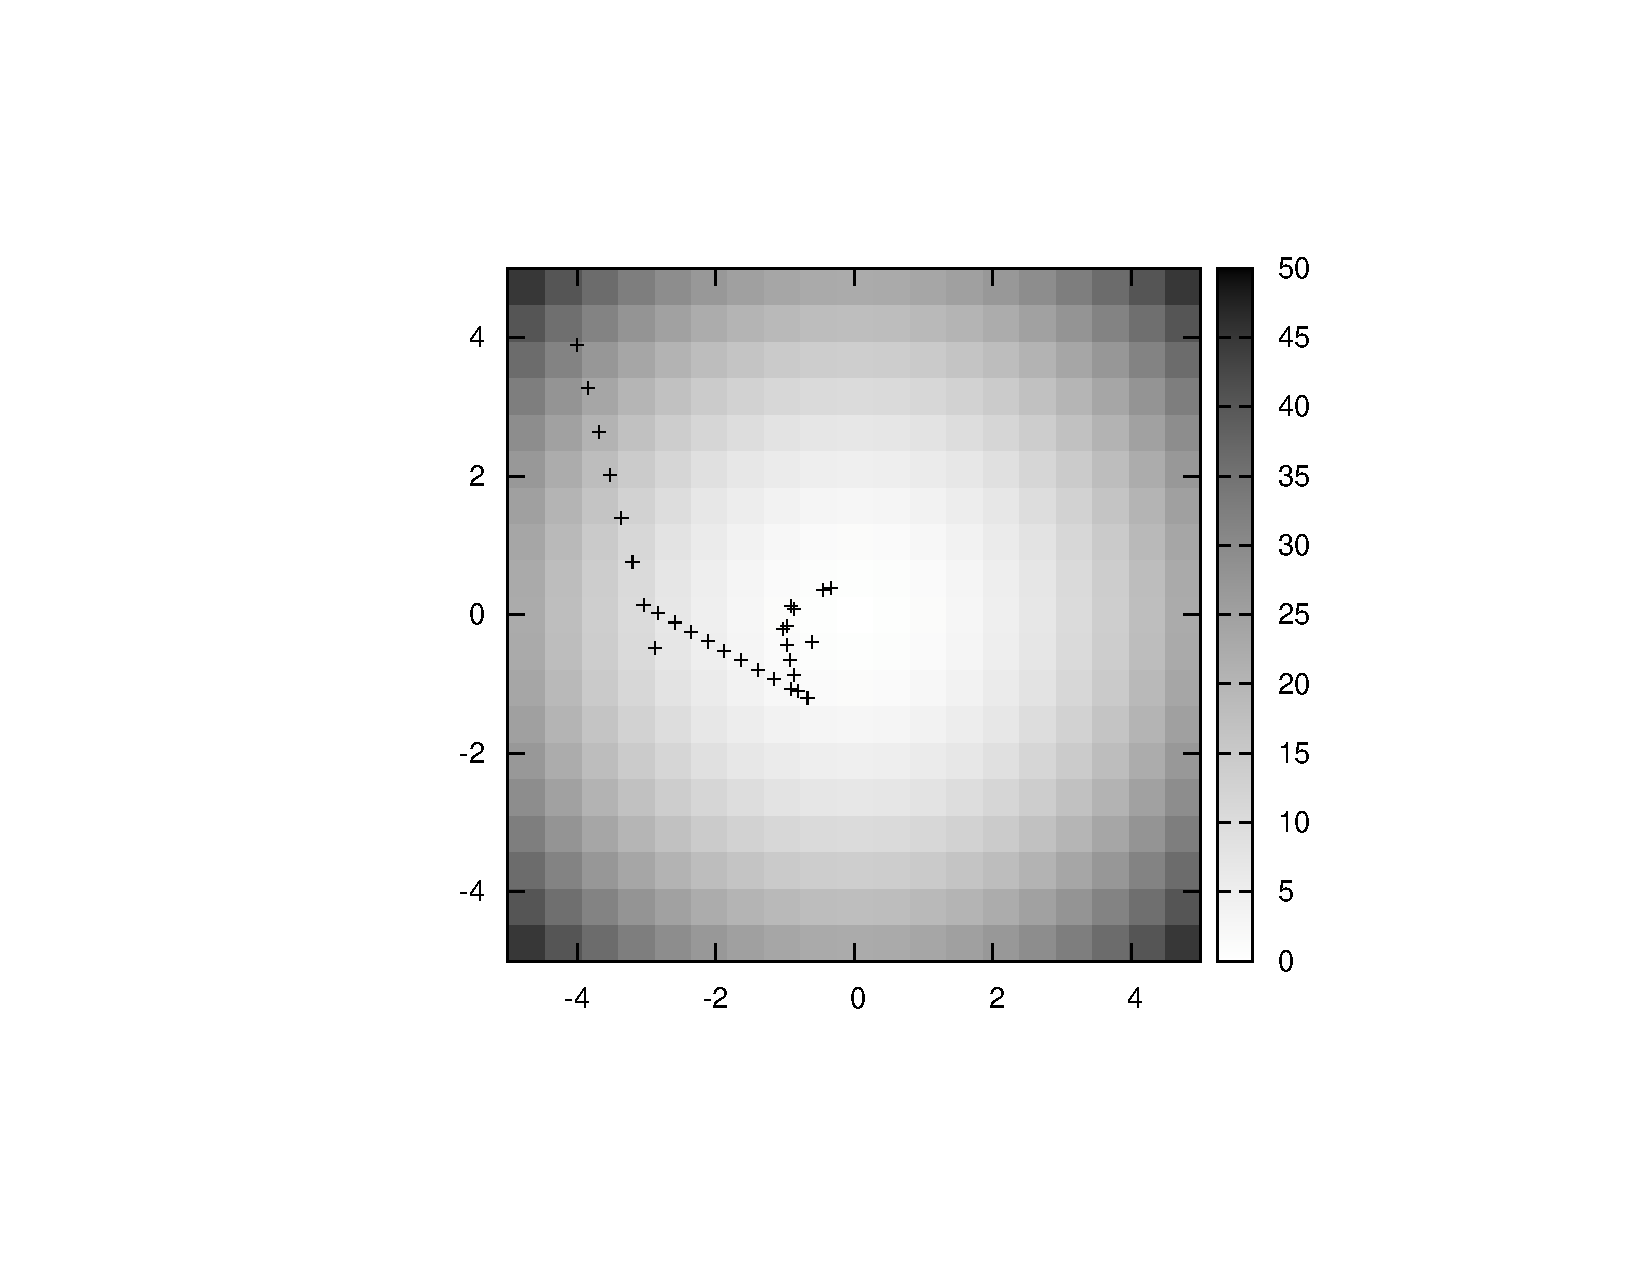
\includegraphics[trim = 2in 1.5in 2in 1.5in, clip, scale=0.5]{graphics/pso1.pdf}
\caption{Heat map plot showing selected samples in the domain.}
\label{plot:pso1}
\end{figure}

\begin{lstlisting}[caption=Gnuplot script use to create a heat map and selected samples., label=pso1]
set xrange [-5:5]
set yrange [-5:5]
set pm3d map
set palette gray negative
set samples 20
set isosamples 20
splot x*x+y*y, "pso1.txt" using 1:2:(0) with points
\end{lstlisting}

\begin{lstlisting}[caption=Snippet of the \texttt{pso1.txt} file., label=pso.file]
-3.9986483808224222 3.8910758979126956 31.12966051677087
-3.838580364459159 3.266132168962991 25.402318559546302
-3.678512348095896 2.6411884400132863 20.507329470753803
-3.518444331732633 2.0162447110635817 16.44469325039336
-3.35837631536937 1.391300982113877 13.214409898464986
...
\end{lstlisting}

% Traveling Salesman Problem
\subsubsection{Traveling Salesman Problem}
% general
Visualizing the results of a combinatorial optimization can provide insight into the areas of the problem that a selected technique is handling well, or  poorly.
Candidate solutions can be visualized over the course of a run to observe how the complexity of solutions found by a technique change over time. Alternatively, the best candidate solutions can be visualized at the end of a run. 

Candidate solutions for the TSP are easily visualized as tours (order of city visits) in the context of the city coordinates of the problem definition.

Figure~\ref{plot:tsp3} provides a plot of an example Nearest-Neighbor solution for the Berlin52 TSP. A Nearest-Neighbor solution is constructed by randomly selecting the first city in the tour then selecting the next city in the tour with the minimum distance to the current city until a complete tour is created. 

\begin{figure}[htp]
\centering
% GNUPLOT: LaTeX picture
\setlength{\unitlength}{0.240900pt}
\ifx\plotpoint\undefined\newsavebox{\plotpoint}\fi
\sbox{\plotpoint}{\rule[-0.200pt]{0.400pt}{0.400pt}}%
\begin{picture}(1500,900)(0,0)
\sbox{\plotpoint}{\rule[-0.200pt]{0.400pt}{0.400pt}}%
\put(190.0,82.0){\rule[-0.200pt]{4.818pt}{0.400pt}}
\put(170,82){\makebox(0,0)[r]{ 0}}
\put(1430.0,82.0){\rule[-0.200pt]{4.818pt}{0.400pt}}
\put(190.0,212.0){\rule[-0.200pt]{4.818pt}{0.400pt}}
\put(170,212){\makebox(0,0)[r]{ 200}}
\put(1430.0,212.0){\rule[-0.200pt]{4.818pt}{0.400pt}}
\put(190.0,341.0){\rule[-0.200pt]{4.818pt}{0.400pt}}
\put(170,341){\makebox(0,0)[r]{ 400}}
\put(1430.0,341.0){\rule[-0.200pt]{4.818pt}{0.400pt}}
\put(190.0,471.0){\rule[-0.200pt]{4.818pt}{0.400pt}}
\put(170,471){\makebox(0,0)[r]{ 600}}
\put(1430.0,471.0){\rule[-0.200pt]{4.818pt}{0.400pt}}
\put(190.0,601.0){\rule[-0.200pt]{4.818pt}{0.400pt}}
\put(170,601){\makebox(0,0)[r]{ 800}}
\put(1430.0,601.0){\rule[-0.200pt]{4.818pt}{0.400pt}}
\put(190.0,730.0){\rule[-0.200pt]{4.818pt}{0.400pt}}
\put(170,730){\makebox(0,0)[r]{ 1000}}
\put(1430.0,730.0){\rule[-0.200pt]{4.818pt}{0.400pt}}
\put(190.0,860.0){\rule[-0.200pt]{4.818pt}{0.400pt}}
\put(170,860){\makebox(0,0)[r]{ 1200}}
\put(1430.0,860.0){\rule[-0.200pt]{4.818pt}{0.400pt}}
\put(190.0,82.0){\rule[-0.200pt]{0.400pt}{4.818pt}}
\put(190,41){\makebox(0,0){ 0}}
\put(190.0,840.0){\rule[-0.200pt]{0.400pt}{4.818pt}}
\put(330.0,82.0){\rule[-0.200pt]{0.400pt}{4.818pt}}
\put(330,41){\makebox(0,0){ 200}}
\put(330.0,840.0){\rule[-0.200pt]{0.400pt}{4.818pt}}
\put(470.0,82.0){\rule[-0.200pt]{0.400pt}{4.818pt}}
\put(470,41){\makebox(0,0){ 400}}
\put(470.0,840.0){\rule[-0.200pt]{0.400pt}{4.818pt}}
\put(610.0,82.0){\rule[-0.200pt]{0.400pt}{4.818pt}}
\put(610,41){\makebox(0,0){ 600}}
\put(610.0,840.0){\rule[-0.200pt]{0.400pt}{4.818pt}}
\put(750.0,82.0){\rule[-0.200pt]{0.400pt}{4.818pt}}
\put(750,41){\makebox(0,0){ 800}}
\put(750.0,840.0){\rule[-0.200pt]{0.400pt}{4.818pt}}
\put(890.0,82.0){\rule[-0.200pt]{0.400pt}{4.818pt}}
\put(890,41){\makebox(0,0){ 1000}}
\put(890.0,840.0){\rule[-0.200pt]{0.400pt}{4.818pt}}
\put(1030.0,82.0){\rule[-0.200pt]{0.400pt}{4.818pt}}
\put(1030,41){\makebox(0,0){ 1200}}
\put(1030.0,840.0){\rule[-0.200pt]{0.400pt}{4.818pt}}
\put(1170.0,82.0){\rule[-0.200pt]{0.400pt}{4.818pt}}
\put(1170,41){\makebox(0,0){ 1400}}
\put(1170.0,840.0){\rule[-0.200pt]{0.400pt}{4.818pt}}
\put(1310.0,82.0){\rule[-0.200pt]{0.400pt}{4.818pt}}
\put(1310,41){\makebox(0,0){ 1600}}
\put(1310.0,840.0){\rule[-0.200pt]{0.400pt}{4.818pt}}
\put(1450.0,82.0){\rule[-0.200pt]{0.400pt}{4.818pt}}
\put(1450,41){\makebox(0,0){ 1800}}
\put(1450.0,840.0){\rule[-0.200pt]{0.400pt}{4.818pt}}
\put(190.0,82.0){\rule[-0.200pt]{0.400pt}{187.420pt}}
\put(190.0,82.0){\rule[-0.200pt]{303.534pt}{0.400pt}}
\put(1450.0,82.0){\rule[-0.200pt]{0.400pt}{187.420pt}}
\put(190.0,860.0){\rule[-0.200pt]{303.534pt}{0.400pt}}
\put(1290,820){\makebox(0,0)[r]{"berlin52.nn.tour"}}
\put(1310.0,820.0){\rule[-0.200pt]{24.090pt}{0.400pt}}
\put(522,704){\usebox{\plotpoint}}
\multiput(522.00,704.58)(0.674,0.497){49}{\rule{0.638pt}{0.120pt}}
\multiput(522.00,703.17)(33.675,26.000){2}{\rule{0.319pt}{0.400pt}}
\multiput(555.92,716.14)(-0.491,-4.196){17}{\rule{0.118pt}{3.340pt}}
\multiput(556.17,723.07)(-10.000,-74.068){2}{\rule{0.400pt}{1.670pt}}
\multiput(547.58,646.50)(0.497,-0.629){59}{\rule{0.120pt}{0.603pt}}
\multiput(546.17,647.75)(31.000,-37.748){2}{\rule{0.400pt}{0.302pt}}
\multiput(578.58,598.08)(0.494,-3.545){25}{\rule{0.119pt}{2.871pt}}
\multiput(577.17,604.04)(14.000,-91.040){2}{\rule{0.400pt}{1.436pt}}
\multiput(592.58,510.53)(0.496,-0.619){39}{\rule{0.119pt}{0.595pt}}
\multiput(591.17,511.76)(21.000,-24.765){2}{\rule{0.400pt}{0.298pt}}
\multiput(611.92,484.69)(-0.497,-0.571){53}{\rule{0.120pt}{0.557pt}}
\multiput(612.17,485.84)(-28.000,-30.844){2}{\rule{0.400pt}{0.279pt}}
\multiput(576.01,455.59)(-2.751,0.482){9}{\rule{2.167pt}{0.116pt}}
\multiput(580.50,454.17)(-26.503,6.000){2}{\rule{1.083pt}{0.400pt}}
\multiput(547.47,459.92)(-1.867,-0.495){35}{\rule{1.574pt}{0.119pt}}
\multiput(550.73,460.17)(-66.734,-19.000){2}{\rule{0.787pt}{0.400pt}}
\multiput(482.94,442.00)(-0.468,7.500){5}{\rule{0.113pt}{5.300pt}}
\multiput(483.17,442.00)(-4.000,41.000){2}{\rule{0.400pt}{2.650pt}}
\multiput(478.92,494.00)(-0.498,0.756){95}{\rule{0.120pt}{0.704pt}}
\multiput(479.17,494.00)(-49.000,72.539){2}{\rule{0.400pt}{0.352pt}}
\multiput(426.36,566.92)(-1.277,-0.499){107}{\rule{1.118pt}{0.120pt}}
\multiput(428.68,567.17)(-137.679,-55.000){2}{\rule{0.559pt}{0.400pt}}
\multiput(291.58,510.60)(0.499,-0.596){215}{\rule{0.120pt}{0.577pt}}
\multiput(290.17,511.80)(109.000,-128.802){2}{\rule{0.400pt}{0.289pt}}
\multiput(400.00,381.92)(1.984,-0.497){61}{\rule{1.675pt}{0.120pt}}
\multiput(400.00,382.17)(122.523,-32.000){2}{\rule{0.838pt}{0.400pt}}
\multiput(526.00,349.92)(0.878,-0.497){61}{\rule{0.800pt}{0.120pt}}
\multiput(526.00,350.17)(54.340,-32.000){2}{\rule{0.400pt}{0.400pt}}
\multiput(582.00,317.94)(3.406,-0.468){5}{\rule{2.500pt}{0.113pt}}
\multiput(582.00,318.17)(18.811,-4.000){2}{\rule{1.250pt}{0.400pt}}
\multiput(606.00,315.59)(6.900,0.485){11}{\rule{5.300pt}{0.117pt}}
\multiput(606.00,314.17)(80.000,7.000){2}{\rule{2.650pt}{0.400pt}}
\multiput(695.92,322.00)(-0.495,2.513){31}{\rule{0.119pt}{2.076pt}}
\multiput(696.17,322.00)(-17.000,79.690){2}{\rule{0.400pt}{1.038pt}}
\multiput(677.76,458.58)(-0.547,0.491){17}{\rule{0.540pt}{0.118pt}}
\multiput(678.88,457.17)(-9.879,10.000){2}{\rule{0.270pt}{0.400pt}}
\put(680.0,406.0){\rule[-0.200pt]{0.400pt}{12.527pt}}
\multiput(669.00,477.58)(0.738,0.495){31}{\rule{0.688pt}{0.119pt}}
\multiput(669.00,476.17)(23.572,17.000){2}{\rule{0.344pt}{0.400pt}}
\multiput(694.00,494.59)(1.601,0.489){15}{\rule{1.344pt}{0.118pt}}
\multiput(694.00,493.17)(25.210,9.000){2}{\rule{0.672pt}{0.400pt}}
\multiput(722.00,501.95)(5.151,-0.447){3}{\rule{3.300pt}{0.108pt}}
\multiput(722.00,502.17)(17.151,-3.000){2}{\rule{1.650pt}{0.400pt}}
\multiput(744.92,497.34)(-0.495,-0.678){31}{\rule{0.119pt}{0.641pt}}
\multiput(745.17,498.67)(-17.000,-21.669){2}{\rule{0.400pt}{0.321pt}}
\put(669.0,468.0){\rule[-0.200pt]{0.400pt}{2.168pt}}
\multiput(771.61,477.00)(0.447,2.025){3}{\rule{0.108pt}{1.433pt}}
\multiput(770.17,477.00)(3.000,7.025){2}{\rule{0.400pt}{0.717pt}}
\multiput(774.59,487.00)(0.485,1.484){11}{\rule{0.117pt}{1.243pt}}
\multiput(773.17,487.00)(7.000,17.420){2}{\rule{0.400pt}{0.621pt}}
\put(729.0,477.0){\rule[-0.200pt]{10.118pt}{0.400pt}}
\multiput(781.00,521.92)(0.972,-0.493){23}{\rule{0.869pt}{0.119pt}}
\multiput(781.00,522.17)(23.196,-13.000){2}{\rule{0.435pt}{0.400pt}}
\multiput(806.00,510.58)(1.426,0.494){29}{\rule{1.225pt}{0.119pt}}
\multiput(806.00,509.17)(42.457,16.000){2}{\rule{0.613pt}{0.400pt}}
\multiput(851.58,520.21)(0.496,-1.637){39}{\rule{0.119pt}{1.395pt}}
\multiput(850.17,523.10)(21.000,-65.104){2}{\rule{0.400pt}{0.698pt}}
\multiput(868.88,456.92)(-0.816,-0.499){121}{\rule{0.752pt}{0.120pt}}
\multiput(870.44,457.17)(-99.440,-62.000){2}{\rule{0.376pt}{0.400pt}}
\multiput(769.92,392.84)(-0.499,-0.828){235}{\rule{0.120pt}{0.762pt}}
\multiput(770.17,394.42)(-119.000,-195.418){2}{\rule{0.400pt}{0.381pt}}
\multiput(645.13,199.58)(-1.955,0.498){87}{\rule{1.656pt}{0.120pt}}
\multiput(648.56,198.17)(-171.564,45.000){2}{\rule{0.828pt}{0.400pt}}
\multiput(424.16,244.59)(-16.816,0.485){11}{\rule{12.729pt}{0.117pt}}
\multiput(450.58,243.17)(-194.581,7.000){2}{\rule{6.364pt}{0.400pt}}
\multiput(251.52,249.92)(-1.237,-0.496){37}{\rule{1.080pt}{0.119pt}}
\multiput(253.76,250.17)(-46.758,-20.000){2}{\rule{0.540pt}{0.400pt}}
\put(781.0,507.0){\rule[-0.200pt]{0.400pt}{3.854pt}}
\multiput(207.00,202.58)(0.625,0.500){949}{\rule{0.600pt}{0.120pt}}
\multiput(207.00,201.17)(593.755,476.000){2}{\rule{0.300pt}{0.400pt}}
\multiput(799.68,678.58)(-0.573,0.499){271}{\rule{0.558pt}{0.120pt}}
\multiput(800.84,677.17)(-155.841,137.000){2}{\rule{0.279pt}{0.400pt}}
\multiput(641.78,815.58)(-0.848,0.497){55}{\rule{0.776pt}{0.120pt}}
\multiput(643.39,814.17)(-47.390,29.000){2}{\rule{0.388pt}{0.400pt}}
\multiput(596.00,842.92)(20.771,-0.491){17}{\rule{16.060pt}{0.118pt}}
\multiput(596.00,843.17)(365.667,-10.000){2}{\rule{8.030pt}{0.400pt}}
\multiput(995.58,830.06)(0.499,-1.061){263}{\rule{0.120pt}{0.948pt}}
\multiput(994.17,832.03)(133.000,-280.032){2}{\rule{0.400pt}{0.474pt}}
\multiput(1126.92,549.73)(-0.499,-0.559){165}{\rule{0.120pt}{0.548pt}}
\multiput(1127.17,550.86)(-84.000,-92.863){2}{\rule{0.400pt}{0.274pt}}
\multiput(1044.58,448.33)(0.496,-2.825){39}{\rule{0.119pt}{2.329pt}}
\multiput(1043.17,453.17)(21.000,-112.167){2}{\rule{0.400pt}{1.164pt}}
\multiput(1065.58,338.72)(0.498,-0.561){95}{\rule{0.120pt}{0.549pt}}
\multiput(1064.17,339.86)(49.000,-53.861){2}{\rule{0.400pt}{0.274pt}}
\multiput(1110.85,284.92)(-0.824,-0.498){87}{\rule{0.758pt}{0.120pt}}
\multiput(1112.43,285.17)(-72.427,-45.000){2}{\rule{0.379pt}{0.400pt}}
\multiput(1038.92,234.32)(-0.497,-1.902){59}{\rule{0.120pt}{1.610pt}}
\multiput(1039.17,237.66)(-31.000,-113.659){2}{\rule{0.400pt}{0.805pt}}
\multiput(1009.00,124.58)(1.173,0.499){173}{\rule{1.036pt}{0.120pt}}
\multiput(1009.00,123.17)(203.849,88.000){2}{\rule{0.518pt}{0.400pt}}
\multiput(1215.58,207.00)(0.498,-1.386){89}{\rule{0.120pt}{1.204pt}}
\multiput(1214.17,209.50)(46.000,-124.500){2}{\rule{0.400pt}{0.602pt}}
\multiput(1261.58,85.00)(0.499,0.530){291}{\rule{0.120pt}{0.524pt}}
\multiput(1260.17,85.00)(147.000,154.911){2}{\rule{0.400pt}{0.262pt}}
\multiput(1406.92,241.00)(-0.499,1.281){187}{\rule{0.120pt}{1.123pt}}
\multiput(1407.17,241.00)(-95.000,240.669){2}{\rule{0.400pt}{0.562pt}}
\multiput(1306.61,484.58)(-1.800,0.500){437}{\rule{1.538pt}{0.120pt}}
\multiput(1309.81,483.17)(-787.807,220.000){2}{\rule{0.769pt}{0.400pt}}
\put(522,704){\raisebox{-.8pt}{\makebox(0,0){$\Diamond$}}}
\put(557,730){\raisebox{-.8pt}{\makebox(0,0){$\Diamond$}}}
\put(547,649){\raisebox{-.8pt}{\makebox(0,0){$\Diamond$}}}
\put(578,610){\raisebox{-.8pt}{\makebox(0,0){$\Diamond$}}}
\put(592,513){\raisebox{-.8pt}{\makebox(0,0){$\Diamond$}}}
\put(613,487){\raisebox{-.8pt}{\makebox(0,0){$\Diamond$}}}
\put(585,455){\raisebox{-.8pt}{\makebox(0,0){$\Diamond$}}}
\put(554,461){\raisebox{-.8pt}{\makebox(0,0){$\Diamond$}}}
\put(484,442){\raisebox{-.8pt}{\makebox(0,0){$\Diamond$}}}
\put(480,494){\raisebox{-.8pt}{\makebox(0,0){$\Diamond$}}}
\put(431,568){\raisebox{-.8pt}{\makebox(0,0){$\Diamond$}}}
\put(291,513){\raisebox{-.8pt}{\makebox(0,0){$\Diamond$}}}
\put(400,383){\raisebox{-.8pt}{\makebox(0,0){$\Diamond$}}}
\put(526,351){\raisebox{-.8pt}{\makebox(0,0){$\Diamond$}}}
\put(582,319){\raisebox{-.8pt}{\makebox(0,0){$\Diamond$}}}
\put(606,315){\raisebox{-.8pt}{\makebox(0,0){$\Diamond$}}}
\put(697,322){\raisebox{-.8pt}{\makebox(0,0){$\Diamond$}}}
\put(680,406){\raisebox{-.8pt}{\makebox(0,0){$\Diamond$}}}
\put(680,458){\raisebox{-.8pt}{\makebox(0,0){$\Diamond$}}}
\put(669,468){\raisebox{-.8pt}{\makebox(0,0){$\Diamond$}}}
\put(669,477){\raisebox{-.8pt}{\makebox(0,0){$\Diamond$}}}
\put(694,494){\raisebox{-.8pt}{\makebox(0,0){$\Diamond$}}}
\put(722,503){\raisebox{-.8pt}{\makebox(0,0){$\Diamond$}}}
\put(746,500){\raisebox{-.8pt}{\makebox(0,0){$\Diamond$}}}
\put(729,477){\raisebox{-.8pt}{\makebox(0,0){$\Diamond$}}}
\put(771,477){\raisebox{-.8pt}{\makebox(0,0){$\Diamond$}}}
\put(774,487){\raisebox{-.8pt}{\makebox(0,0){$\Diamond$}}}
\put(781,507){\raisebox{-.8pt}{\makebox(0,0){$\Diamond$}}}
\put(781,523){\raisebox{-.8pt}{\makebox(0,0){$\Diamond$}}}
\put(806,510){\raisebox{-.8pt}{\makebox(0,0){$\Diamond$}}}
\put(851,526){\raisebox{-.8pt}{\makebox(0,0){$\Diamond$}}}
\put(872,458){\raisebox{-.8pt}{\makebox(0,0){$\Diamond$}}}
\put(771,396){\raisebox{-.8pt}{\makebox(0,0){$\Diamond$}}}
\put(652,199){\raisebox{-.8pt}{\makebox(0,0){$\Diamond$}}}
\put(477,244){\raisebox{-.8pt}{\makebox(0,0){$\Diamond$}}}
\put(256,251){\raisebox{-.8pt}{\makebox(0,0){$\Diamond$}}}
\put(207,231){\raisebox{-.8pt}{\makebox(0,0){$\Diamond$}}}
\put(207,202){\raisebox{-.8pt}{\makebox(0,0){$\Diamond$}}}
\put(802,678){\raisebox{-.8pt}{\makebox(0,0){$\Diamond$}}}
\put(645,815){\raisebox{-.8pt}{\makebox(0,0){$\Diamond$}}}
\put(596,844){\raisebox{-.8pt}{\makebox(0,0){$\Diamond$}}}
\put(995,834){\raisebox{-.8pt}{\makebox(0,0){$\Diamond$}}}
\put(1128,552){\raisebox{-.8pt}{\makebox(0,0){$\Diamond$}}}
\put(1044,458){\raisebox{-.8pt}{\makebox(0,0){$\Diamond$}}}
\put(1065,341){\raisebox{-.8pt}{\makebox(0,0){$\Diamond$}}}
\put(1114,286){\raisebox{-.8pt}{\makebox(0,0){$\Diamond$}}}
\put(1040,241){\raisebox{-.8pt}{\makebox(0,0){$\Diamond$}}}
\put(1009,124){\raisebox{-.8pt}{\makebox(0,0){$\Diamond$}}}
\put(1215,212){\raisebox{-.8pt}{\makebox(0,0){$\Diamond$}}}
\put(1261,85){\raisebox{-.8pt}{\makebox(0,0){$\Diamond$}}}
\put(1408,241){\raisebox{-.8pt}{\makebox(0,0){$\Diamond$}}}
\put(1313,484){\raisebox{-.8pt}{\makebox(0,0){$\Diamond$}}}
\put(522,704){\raisebox{-.8pt}{\makebox(0,0){$\Diamond$}}}
\put(1360,820){\raisebox{-.8pt}{\makebox(0,0){$\Diamond$}}}
\put(207.0,202.0){\rule[-0.200pt]{0.400pt}{6.986pt}}
\put(190.0,82.0){\rule[-0.200pt]{0.400pt}{187.420pt}}
\put(190.0,82.0){\rule[-0.200pt]{303.534pt}{0.400pt}}
\put(1450.0,82.0){\rule[-0.200pt]{0.400pt}{187.420pt}}
\put(190.0,860.0){\rule[-0.200pt]{303.534pt}{0.400pt}}
\end{picture}

\caption{Plot of a Nearest-Neighbor tour for the Berlin52 TSP.}
\label{plot:tsp3}
\end{figure}

Listing~\ref{tsp3} provides the Gnuplot script used to prepare the plot, where \texttt{berlin52.nn.tour} is a file that contains a listing of the coordinates of all cities separated by white space in order that the cities are visited with one city per line. The first city in the tour is repeated as the last city in the tour to provide a closed polygon in the plot.
Listing~\ref{tsp3.file} provides a snippet of the first five lines of the \texttt{berlin52.nn.tour} file.

\begin{lstlisting}[caption=Gnuplot script for plotting a tour for a TSP., label=tsp3]
plot "berlin52.nn.tour" with linespoints
\end{lstlisting}

\begin{lstlisting}[caption=Snippet of the berlin52.nn.tour file., label=tsp3.file]
475 960
525 1000
510 875
555 815
575 665
...
\end{lstlisting}

Figure~\ref{plot:tsp2} provides a plot of the known optimal solution for the Berlin52 Traveling Salesman problem. 

\begin{figure}[htp]
\centering
% GNUPLOT: LaTeX picture
\setlength{\unitlength}{0.240900pt}
\ifx\plotpoint\undefined\newsavebox{\plotpoint}\fi
\sbox{\plotpoint}{\rule[-0.200pt]{0.400pt}{0.400pt}}%
\begin{picture}(1500,900)(0,0)
\sbox{\plotpoint}{\rule[-0.200pt]{0.400pt}{0.400pt}}%
\put(150.0,82.0){\rule[-0.200pt]{4.818pt}{0.400pt}}
\put(130,82){\makebox(0,0)[r]{ 0}}
\put(1419.0,82.0){\rule[-0.200pt]{4.818pt}{0.400pt}}
\put(150.0,212.0){\rule[-0.200pt]{4.818pt}{0.400pt}}
\put(130,212){\makebox(0,0)[r]{ 200}}
\put(1419.0,212.0){\rule[-0.200pt]{4.818pt}{0.400pt}}
\put(150.0,341.0){\rule[-0.200pt]{4.818pt}{0.400pt}}
\put(130,341){\makebox(0,0)[r]{ 400}}
\put(1419.0,341.0){\rule[-0.200pt]{4.818pt}{0.400pt}}
\put(150.0,471.0){\rule[-0.200pt]{4.818pt}{0.400pt}}
\put(130,471){\makebox(0,0)[r]{ 600}}
\put(1419.0,471.0){\rule[-0.200pt]{4.818pt}{0.400pt}}
\put(150.0,600.0){\rule[-0.200pt]{4.818pt}{0.400pt}}
\put(130,600){\makebox(0,0)[r]{ 800}}
\put(1419.0,600.0){\rule[-0.200pt]{4.818pt}{0.400pt}}
\put(150.0,730.0){\rule[-0.200pt]{4.818pt}{0.400pt}}
\put(130,730){\makebox(0,0)[r]{ 1000}}
\put(1419.0,730.0){\rule[-0.200pt]{4.818pt}{0.400pt}}
\put(150.0,859.0){\rule[-0.200pt]{4.818pt}{0.400pt}}
\put(130,859){\makebox(0,0)[r]{ 1200}}
\put(1419.0,859.0){\rule[-0.200pt]{4.818pt}{0.400pt}}
\put(150.0,82.0){\rule[-0.200pt]{0.400pt}{4.818pt}}
\put(150,41){\makebox(0,0){ 0}}
\put(150.0,839.0){\rule[-0.200pt]{0.400pt}{4.818pt}}
\put(293.0,82.0){\rule[-0.200pt]{0.400pt}{4.818pt}}
\put(293,41){\makebox(0,0){ 200}}
\put(293.0,839.0){\rule[-0.200pt]{0.400pt}{4.818pt}}
\put(436.0,82.0){\rule[-0.200pt]{0.400pt}{4.818pt}}
\put(436,41){\makebox(0,0){ 400}}
\put(436.0,839.0){\rule[-0.200pt]{0.400pt}{4.818pt}}
\put(580.0,82.0){\rule[-0.200pt]{0.400pt}{4.818pt}}
\put(580,41){\makebox(0,0){ 600}}
\put(580.0,839.0){\rule[-0.200pt]{0.400pt}{4.818pt}}
\put(723.0,82.0){\rule[-0.200pt]{0.400pt}{4.818pt}}
\put(723,41){\makebox(0,0){ 800}}
\put(723.0,839.0){\rule[-0.200pt]{0.400pt}{4.818pt}}
\put(866.0,82.0){\rule[-0.200pt]{0.400pt}{4.818pt}}
\put(866,41){\makebox(0,0){ 1000}}
\put(866.0,839.0){\rule[-0.200pt]{0.400pt}{4.818pt}}
\put(1009.0,82.0){\rule[-0.200pt]{0.400pt}{4.818pt}}
\put(1009,41){\makebox(0,0){ 1200}}
\put(1009.0,839.0){\rule[-0.200pt]{0.400pt}{4.818pt}}
\put(1153.0,82.0){\rule[-0.200pt]{0.400pt}{4.818pt}}
\put(1153,41){\makebox(0,0){ 1400}}
\put(1153.0,839.0){\rule[-0.200pt]{0.400pt}{4.818pt}}
\put(1296.0,82.0){\rule[-0.200pt]{0.400pt}{4.818pt}}
\put(1296,41){\makebox(0,0){ 1600}}
\put(1296.0,839.0){\rule[-0.200pt]{0.400pt}{4.818pt}}
\put(1439.0,82.0){\rule[-0.200pt]{0.400pt}{4.818pt}}
\put(1439,41){\makebox(0,0){ 1800}}
\put(1439.0,839.0){\rule[-0.200pt]{0.400pt}{4.818pt}}
\put(150.0,82.0){\rule[-0.200pt]{0.400pt}{187.179pt}}
\put(150.0,82.0){\rule[-0.200pt]{310.520pt}{0.400pt}}
\put(1439.0,82.0){\rule[-0.200pt]{0.400pt}{187.179pt}}
\put(150.0,859.0){\rule[-0.200pt]{310.520pt}{0.400pt}}
\put(1279,819){\makebox(0,0)[r]{"./berlin52.optimal"}}
\put(1299.0,819.0){\rule[-0.200pt]{24.090pt}{0.400pt}}
\put(555,454){\usebox{\plotpoint}}
\multiput(555.58,454.00)(0.497,0.589){53}{\rule{0.120pt}{0.571pt}}
\multiput(554.17,454.00)(28.000,31.814){2}{\rule{0.400pt}{0.286pt}}
\multiput(581.92,487.00)(-0.496,0.619){39}{\rule{0.119pt}{0.595pt}}
\multiput(582.17,487.00)(-21.000,24.765){2}{\rule{0.400pt}{0.298pt}}
\multiput(560.92,513.00)(-0.494,3.302){27}{\rule{0.119pt}{2.687pt}}
\multiput(561.17,513.00)(-15.000,91.424){2}{\rule{0.400pt}{1.343pt}}
\multiput(545.92,610.00)(-0.497,0.609){61}{\rule{0.120pt}{0.588pt}}
\multiput(546.17,610.00)(-32.000,37.781){2}{\rule{0.400pt}{0.294pt}}
\multiput(513.92,649.00)(-0.497,1.107){47}{\rule{0.120pt}{0.980pt}}
\multiput(514.17,649.00)(-25.000,52.966){2}{\rule{0.400pt}{0.490pt}}
\multiput(490.00,704.58)(0.693,0.497){49}{\rule{0.654pt}{0.120pt}}
\multiput(490.00,703.17)(34.643,26.000){2}{\rule{0.327pt}{0.400pt}}
\multiput(526.58,730.00)(0.498,1.456){75}{\rule{0.120pt}{1.259pt}}
\multiput(525.17,730.00)(39.000,110.387){2}{\rule{0.400pt}{0.629pt}}
\multiput(565.00,841.92)(0.865,-0.497){55}{\rule{0.790pt}{0.120pt}}
\multiput(565.00,842.17)(48.361,-29.000){2}{\rule{0.395pt}{0.400pt}}
\multiput(615.00,812.92)(0.596,-0.499){269}{\rule{0.576pt}{0.120pt}}
\multiput(615.00,813.17)(160.804,-136.000){2}{\rule{0.288pt}{0.400pt}}
\multiput(777.00,678.58)(0.636,0.499){307}{\rule{0.608pt}{0.120pt}}
\multiput(777.00,677.17)(195.737,155.000){2}{\rule{0.304pt}{0.400pt}}
\multiput(974.58,829.14)(0.499,-1.038){269}{\rule{0.120pt}{0.929pt}}
\multiput(973.17,831.07)(136.000,-280.071){2}{\rule{0.400pt}{0.465pt}}
\multiput(1110.00,549.92)(1.394,-0.499){133}{\rule{1.212pt}{0.120pt}}
\multiput(1110.00,550.17)(186.485,-68.000){2}{\rule{0.606pt}{0.400pt}}
\multiput(1299.58,478.44)(0.499,-1.250){191}{\rule{0.120pt}{1.098pt}}
\multiput(1298.17,480.72)(97.000,-239.721){2}{\rule{0.400pt}{0.549pt}}
\multiput(1394.92,238.86)(-0.499,-0.520){297}{\rule{0.120pt}{0.516pt}}
\multiput(1395.17,239.93)(-150.000,-154.929){2}{\rule{0.400pt}{0.258pt}}
\multiput(1244.92,85.00)(-0.498,1.357){91}{\rule{0.120pt}{1.181pt}}
\multiput(1245.17,85.00)(-47.000,124.549){2}{\rule{0.400pt}{0.590pt}}
\multiput(1194.60,210.92)(-1.201,-0.499){173}{\rule{1.059pt}{0.120pt}}
\multiput(1196.80,211.17)(-208.802,-88.000){2}{\rule{0.530pt}{0.400pt}}
\multiput(988.58,124.00)(0.497,1.842){61}{\rule{0.120pt}{1.562pt}}
\multiput(987.17,124.00)(32.000,113.757){2}{\rule{0.400pt}{0.781pt}}
\multiput(1020.00,241.58)(0.835,0.498){87}{\rule{0.767pt}{0.120pt}}
\multiput(1020.00,240.17)(73.409,45.000){2}{\rule{0.383pt}{0.400pt}}
\multiput(1093.92,286.00)(-0.498,0.550){97}{\rule{0.120pt}{0.540pt}}
\multiput(1094.17,286.00)(-50.000,53.879){2}{\rule{0.400pt}{0.270pt}}
\multiput(1043.92,341.00)(-0.496,2.825){39}{\rule{0.119pt}{2.329pt}}
\multiput(1044.17,341.00)(-21.000,112.167){2}{\rule{0.400pt}{1.164pt}}
\multiput(846.92,458.00)(-0.496,1.637){39}{\rule{0.119pt}{1.395pt}}
\multiput(847.17,458.00)(-21.000,65.104){2}{\rule{0.400pt}{0.698pt}}
\multiput(821.99,524.92)(-1.400,-0.495){31}{\rule{1.206pt}{0.119pt}}
\multiput(824.50,525.17)(-44.497,-17.000){2}{\rule{0.603pt}{0.400pt}}
\multiput(776.39,509.58)(-0.972,0.493){23}{\rule{0.869pt}{0.119pt}}
\multiput(778.20,508.17)(-23.196,13.000){2}{\rule{0.435pt}{0.400pt}}
\put(848.0,458.0){\rule[-0.200pt]{42.398pt}{0.400pt}}
\multiput(753.93,501.08)(-0.485,-1.408){11}{\rule{0.117pt}{1.186pt}}
\multiput(754.17,503.54)(-7.000,-16.539){2}{\rule{0.400pt}{0.593pt}}
\multiput(746.94,482.43)(-0.468,-1.358){5}{\rule{0.113pt}{1.100pt}}
\multiput(747.17,484.72)(-4.000,-7.717){2}{\rule{0.400pt}{0.550pt}}
\multiput(741.78,477.58)(-0.542,0.496){43}{\rule{0.535pt}{0.120pt}}
\multiput(742.89,476.17)(-23.890,23.000){2}{\rule{0.267pt}{0.400pt}}
\multiput(717.92,497.46)(-0.495,-0.639){33}{\rule{0.119pt}{0.611pt}}
\multiput(718.17,498.73)(-18.000,-21.732){2}{\rule{0.400pt}{0.306pt}}
\multiput(699.93,477.00)(-0.485,1.942){11}{\rule{0.117pt}{1.586pt}}
\multiput(700.17,477.00)(-7.000,22.709){2}{\rule{0.400pt}{0.793pt}}
\multiput(688.94,501.92)(-1.433,-0.491){17}{\rule{1.220pt}{0.118pt}}
\multiput(691.47,502.17)(-25.468,-10.000){2}{\rule{0.610pt}{0.400pt}}
\multiput(662.99,491.92)(-0.785,-0.494){29}{\rule{0.725pt}{0.119pt}}
\multiput(664.50,492.17)(-23.495,-16.000){2}{\rule{0.363pt}{0.400pt}}
\put(755.0,506.0){\rule[-0.200pt]{0.400pt}{3.854pt}}
\multiput(641.00,465.93)(0.553,-0.489){15}{\rule{0.544pt}{0.118pt}}
\multiput(641.00,466.17)(8.870,-9.000){2}{\rule{0.272pt}{0.400pt}}
\put(641.0,467.0){\rule[-0.200pt]{0.400pt}{2.409pt}}
\multiput(651.00,404.92)(4.821,-0.491){17}{\rule{3.820pt}{0.118pt}}
\multiput(651.00,405.17)(85.071,-10.000){2}{\rule{1.910pt}{0.400pt}}
\multiput(741.90,394.92)(-0.506,-0.499){145}{\rule{0.505pt}{0.120pt}}
\multiput(742.95,395.17)(-73.951,-74.000){2}{\rule{0.253pt}{0.400pt}}
\multiput(667.92,317.15)(-0.498,-1.343){89}{\rule{0.120pt}{1.170pt}}
\multiput(668.17,319.57)(-46.000,-120.573){2}{\rule{0.400pt}{0.585pt}}
\multiput(621.92,199.00)(-0.498,1.239){91}{\rule{0.120pt}{1.087pt}}
\multiput(622.17,199.00)(-47.000,113.743){2}{\rule{0.400pt}{0.544pt}}
\multiput(561.75,315.61)(-5.374,0.447){3}{\rule{3.433pt}{0.108pt}}
\multiput(568.87,314.17)(-17.874,3.000){2}{\rule{1.717pt}{0.400pt}}
\multiput(547.72,318.58)(-0.866,0.497){63}{\rule{0.791pt}{0.120pt}}
\multiput(549.36,317.17)(-55.358,33.000){2}{\rule{0.395pt}{0.400pt}}
\multiput(492.92,347.03)(-0.498,-1.073){97}{\rule{0.120pt}{0.956pt}}
\multiput(493.17,349.02)(-50.000,-105.016){2}{\rule{0.400pt}{0.478pt}}
\multiput(432.67,242.92)(-3.308,-0.498){81}{\rule{2.729pt}{0.120pt}}
\multiput(438.34,243.17)(-270.337,-42.000){2}{\rule{1.364pt}{0.400pt}}
\put(651.0,406.0){\rule[-0.200pt]{0.400pt}{12.527pt}}
\multiput(168.00,231.58)(1.330,0.495){35}{\rule{1.153pt}{0.119pt}}
\multiput(168.00,230.17)(47.608,19.000){2}{\rule{0.576pt}{0.400pt}}
\multiput(218.00,250.58)(0.552,0.499){263}{\rule{0.542pt}{0.120pt}}
\multiput(218.00,249.17)(145.875,133.000){2}{\rule{0.271pt}{0.400pt}}
\multiput(363.92,383.00)(-0.499,0.586){219}{\rule{0.120pt}{0.568pt}}
\multiput(364.17,383.00)(-111.000,128.820){2}{\rule{0.400pt}{0.284pt}}
\multiput(254.00,513.58)(1.304,0.499){107}{\rule{1.140pt}{0.120pt}}
\multiput(254.00,512.17)(140.634,55.000){2}{\rule{0.570pt}{0.400pt}}
\multiput(397.58,565.09)(0.498,-0.751){97}{\rule{0.120pt}{0.700pt}}
\multiput(396.17,566.55)(50.000,-73.547){2}{\rule{0.400pt}{0.350pt}}
\multiput(447.60,471.00)(0.468,-7.500){5}{\rule{0.113pt}{5.300pt}}
\multiput(446.17,482.00)(4.000,-41.000){2}{\rule{0.400pt}{2.650pt}}
\multiput(451.00,441.58)(1.797,0.496){37}{\rule{1.520pt}{0.119pt}}
\multiput(451.00,440.17)(67.845,20.000){2}{\rule{0.760pt}{0.400pt}}
\multiput(522.00,459.93)(2.476,-0.485){11}{\rule{1.986pt}{0.117pt}}
\multiput(522.00,460.17)(28.879,-7.000){2}{\rule{0.993pt}{0.400pt}}
\put(555,454){\makebox(0,0){$+$}}
\put(583,487){\makebox(0,0){$+$}}
\put(562,513){\makebox(0,0){$+$}}
\put(547,610){\makebox(0,0){$+$}}
\put(515,649){\makebox(0,0){$+$}}
\put(490,704){\makebox(0,0){$+$}}
\put(526,730){\makebox(0,0){$+$}}
\put(565,843){\makebox(0,0){$+$}}
\put(615,814){\makebox(0,0){$+$}}
\put(777,678){\makebox(0,0){$+$}}
\put(974,833){\makebox(0,0){$+$}}
\put(1110,551){\makebox(0,0){$+$}}
\put(1299,483){\makebox(0,0){$+$}}
\put(1396,241){\makebox(0,0){$+$}}
\put(1246,85){\makebox(0,0){$+$}}
\put(1199,212){\makebox(0,0){$+$}}
\put(988,124){\makebox(0,0){$+$}}
\put(1020,241){\makebox(0,0){$+$}}
\put(1095,286){\makebox(0,0){$+$}}
\put(1045,341){\makebox(0,0){$+$}}
\put(1024,458){\makebox(0,0){$+$}}
\put(848,458){\makebox(0,0){$+$}}
\put(827,526){\makebox(0,0){$+$}}
\put(780,509){\makebox(0,0){$+$}}
\put(755,522){\makebox(0,0){$+$}}
\put(755,506){\makebox(0,0){$+$}}
\put(748,487){\makebox(0,0){$+$}}
\put(744,477){\makebox(0,0){$+$}}
\put(719,500){\makebox(0,0){$+$}}
\put(701,477){\makebox(0,0){$+$}}
\put(694,503){\makebox(0,0){$+$}}
\put(666,493){\makebox(0,0){$+$}}
\put(641,477){\makebox(0,0){$+$}}
\put(641,467){\makebox(0,0){$+$}}
\put(651,458){\makebox(0,0){$+$}}
\put(651,406){\makebox(0,0){$+$}}
\put(744,396){\makebox(0,0){$+$}}
\put(669,322){\makebox(0,0){$+$}}
\put(623,199){\makebox(0,0){$+$}}
\put(576,315){\makebox(0,0){$+$}}
\put(551,318){\makebox(0,0){$+$}}
\put(494,351){\makebox(0,0){$+$}}
\put(444,244){\makebox(0,0){$+$}}
\put(168,202){\makebox(0,0){$+$}}
\put(168,231){\makebox(0,0){$+$}}
\put(218,250){\makebox(0,0){$+$}}
\put(365,383){\makebox(0,0){$+$}}
\put(254,513){\makebox(0,0){$+$}}
\put(397,568){\makebox(0,0){$+$}}
\put(447,493){\makebox(0,0){$+$}}
\put(451,441){\makebox(0,0){$+$}}
\put(522,461){\makebox(0,0){$+$}}
\put(555,454){\makebox(0,0){$+$}}
\put(1349,819){\makebox(0,0){$+$}}
\put(168.0,202.0){\rule[-0.200pt]{0.400pt}{6.986pt}}
\put(150.0,82.0){\rule[-0.200pt]{0.400pt}{187.179pt}}
\put(150.0,82.0){\rule[-0.200pt]{310.520pt}{0.400pt}}
\put(1439.0,82.0){\rule[-0.200pt]{0.400pt}{187.179pt}}
\put(150.0,859.0){\rule[-0.200pt]{310.520pt}{0.400pt}}
\end{picture}

\caption{Plot of the optimal tour for the Berlin52 TSP.}
\label{plot:tsp2}
\end{figure}

Listing~\ref{tsp2} provides the Gnuplot script used to prepare the plot, where \texttt{berlin52.optimal} is a file that contains a listing of the coordinates of all cities in order that the cities are visited with one city per line separated by white space. The first city in the tour is repeated as the last city in the tour to provide a closed polygon in the plot.

\begin{lstlisting}[caption=Gnuplot script for plotting a tour for a TSP., label=tsp2]
plot "berlin52.optimal" with linespoints
\end{lstlisting}

Listing~\ref{tsp2.file} provides a snippet of the first five lines of the \texttt{berlin52.optimal} file.

\begin{lstlisting}[caption=Snippet of the \texttt{berlin52.optimal} file., label=tsp2.file]
565.0 575.0
605.0 625.0
575.0 665.0
555.0 815.0
510.0 875.0
...
\end{lstlisting}
\putbib\end{bibunit}
\newpage\begin{bibunit}% The Clever Algorithms Project: http://www.CleverAlgorithms.com
% (c) Copyright 2010 Jason Brownlee. Some Rights Reserved. 
% This work is licensed under a Creative Commons Attribution-Noncommercial-Share Alike 2.5 Australia License.

% Problem Solving Method
\section{Problem Solving Strategies} 
\label{advanced:sec:problem_solving}
\index{Problem Solving Strategies}

% this section
The field of Data Mining has clear methodologies that guide a practitioner to solve problems, such as Knowledge Discovery in Databases (KDD) \cite{Fayyad1996}. Metaheuristics and Computational Intelligence algorithms have no such methodology.\footnote{Some methods can be used for classification and regression and as such may fit into methodologies such as KDD.}

This section describes some of the considerations when applying algorithms from the fields of Metaheuristics, Computational Intelligence, and Biologically Inspired Computation to practical problem domains. This discussion includes:

\begin{itemize} 
  \item The suitability of application of a given technique to a given problem and the transferability of algorithm and problem features (Section~\ref{sec:suitability})
  \item The distinction between strong and weak methods which use more or less problem specific information respectively, and the continuum between these extremes (Section~\ref{sec:strong_methods}).
	\item A summary of problem solving strategies that suggest different ways of applying a given technique to the function optimization and approximation fields (Section~\ref{sec:strategies}).
\end{itemize}

%
% Suitability of Application
%
\subsection{Suitability of Application}
\label{sec:suitability}
\index{Suitability of Application}
% utility as problems solvers
From a problem-solving perspective, the tools that emerge from the field of Computational Intelligence are generally assessed with regard to their utility as \emph{efficiently} or \emph{effectively} solving problems.
% nfl
An important lesson from the No-Free-Lunch Theorem was to \emph{bound claims of applicability} (see Section~{subsec:nfl}), that is to consider the suitability of a given strategy with regard to the feature overlap with the attributes of a given problem domain. From a Computational Intelligence perspective, one may consider the architecture, processes, and constraints of a given strategy as the features of an approach. 

The suitability of the application of a particular approach to a problem takes into considerations concerns such as the \emph{appropriateness} (can the approach address the problem), the \emph{feasibility} (available resources and related efficiency concerns), and the \emph{flexibility} (ability to address unexpected or unintended effects).
% my approach
This section summarizes a general methodology toward addressing the problem of suitability in the context of Computational Intelligence tools. This methodology involves 1) the systematic elicitation of system and problem features, and 2) the consideration of the overlap of problem-problem, algorithm-algorithm, and problem-algorithm overlap of feature sets. 

% Systematic Feature Elicitation
\subsubsection{Systematic Feature Elicitation}
A \emph{feature} of a system (tool, strategy, model) or a problem is a distinctive element or property that may be used to differentiate it from similar and/or related cases. Examples may include functional concerns such as: processes, data structures, architectures, and constraints, as well as emergent concerns that may have a more subjective quality such as general behaviors, organizations, and higher-order structures. The process of the elicitation of features may be taken from a system or problem perspective:

\begin{itemize}
	\item \emph{System Perspective}: This requires a strong focus on the lower level functional elements and investigations that work toward correlating specific controlled procedures towards predictable emergent behaviors. 
	\item \emph{Problem Perspective}: May require both a generalization of the specific case to the general problem case, as well as a functional or logical decomposition into constituent parts.
\end{itemize}

Problem \emph{generalization} and \emph{functional decomposition} are important and commonly used patterns for problem solving in the broader fields of Artificial Intelligence and Machine Learning. The promotion of simplification and modularity can reduce the cost and complexity of achieving solutions \cite{Russell2009, Brooks1986}.

%
% Feature Overlap
%
\subsubsection{Feature Overlap}
% general overlap
Overlap in elicited features may be considered from three important perspectives: \emph{between systems}, \emph{between problems}, and \emph{between a system and a problem}. Further, such overlap may be considered at different levels of detail with regard to generalized problem solving strategies and problem definitions.
% cases
These overlap cases are considered as follows:

\begin{itemize}
	\item \emph{System Overlap} defines the suitability of comparing one system to another, referred to as \emph{comparability}. For example, systems may be considered for the same general problems and compared in terms of theoretical or empirical capability, the results of which may only be meaningful if the systems are significantly similar to each other as assessed in terms of feature overlap. 
	\item \emph{Problem Overlap} defines the suitability of comparing one problem to another, referred to as \emph{transferability}. From a systems focus, transferability refers to the capability of a technique on a given problem to be successfully applied to another problem, the result of which is only meaningful if there is a strong overlap between the problems under consideration.
	\item \emph{System-Problem Overlap} defines the suitability of a system on a given problem, referred to as \emph{applicability}. For example, a system is considered suitable for a given problem if it has a significant overlap in capabilities with the requirements of the problem definition.
\end{itemize}

% noise
Such mappings are imprecise given the subjective assessment and complexity required in both the elicitation and consideration overlap of the of features, the hardest of which is expected to be the mapping between systems and problems. 
% nfl
The mapping of salient features of algorithms and problems was proposed as an important reconciliation of the No-Free-Lunch Theorem by Wolpert and Macready \cite{Wolpert1997}, although the important difference of this approach is that the system and algorithm are given prior to the assessment. In their first work on the theorem, Wolpert and Macready specifically propose the elicitation of the features from a problem-first perspective, for which specialized algorithms can be defined \cite{Wolpert1995}. Therefore, this methodology of suitability may be considered a generalization of this reconciliation suitable for the altered Computational Intelligence (strategy first) perspective on Artificial Intelligence.
% this argument also supports outlining capability by analogy

%
% Strong and Weak Methods
%
\subsection{Strong and Weak Methods}
\label{sec:strong_methods}
\index{Strong and Weak Methods}
% weak
Generally, the methods from the fields of Metaheuristics, Computational Intelligence, and Biologically Inspired Computation may be considered weak methods. They are general purpose and are typically considered black-box solvers for a range of problem domains. The stronger the method, the more that must be known about the problem domain.
% weak and strong
Rather than discriminating techniques into weak and strong it is more useful to consider a continuum of methods from pure block box techniques that have few assumptions about the problem domain, to strong methods that exploit most or all of the problem specific information available.

For example, the Traveling Salesman Problem is an example of a combinatorial optimization problem. A na\"ive (such a Random Search) black box method may simply explore permutations of the cities. Slightly stronger methods may initialize the search with a heuristic-generated technique (such as nearest neighbor) and explore the search space using a variation method that also exploits heuristic information about the domain (such as a 2-opt variation). Continuing along this theme, a stochastic method may explore the search space using a combination of probabilistic and heuristic information (such as Ant Colony Optimization algorithms). At the other end of the scale the stochastic elements are decreased or removed until one is left with pure heuristic methods such as  the Lin-Kernighan heuristic \cite{Lin1973} and exact algorithms from linear and dynamic programming that focus on the structure and nature of the problem \cite{Woeginger2003}.

% strategy
Approaching a problem is not as simple as selecting the strongest method available and solving it. The following describes two potential strategies:

\begin{itemize}
  \item \emph{Start Strong}: Select the strongest technique available and apply it to the problem. Difficult problems can be resistant to traditional methods for many intrinsic and extrinsic reasons. Use products from a strong technique (best solution found, heuristics) to seed the next weaker method in line. 
  \item \emph{Start Weak}: Strong methods do not exist for all problems, and if they do exist, the computation, skill, and/or time resources may not be available to exploit them. Start with a weak technique and use it to learn about the problem domain. Use this information to make better decisions about subsequent techniques to try that can exploit what has been learned.
\end{itemize}

In a real-world engineering or business scenario, the objective is to solve a problem or achieve the best possible solution to the problem within the operating constraints.
Concerns of algorithm and technique purity become less important than they may be in their respective fields of research.
Both of the above strategies suggest an iterative methodology, where the product or knowledge gained from one technique may be used to prime a subsequent stronger or weaker technique. 

%
% Domain-Specific Strategies
%
\subsection{Domain-Specific Strategies}
\label{sec:strategies}
\index{Domain-Specific Strategies}
An algorithm may be considered a strategy for problem solving. There are a wide range of ways in which a given algorithm can be used to solve a problem. 
Function Optimization and Function Approximation were presented as two general classes of problems to which the algorithms from the fields of Metaheuristics, Computational Intelligence, and Biologically Inspired Computation are applied. 
This section reviews general problem problem solving strategies that may be adopted for a given technique in each of these general problem domains.

%
% Function Optimization
%
\subsubsection{Function Optimization}
\index{Function Optimization}
This section reviews a select set of strategies for addressing optimization problems from the field of Metaheuristics and Computational Intelligence to provide general insight into the state of the interaction between stochastic algorithms and the field of optimization. This section draws heavily from the field of Evolutionary Computation, Swarm Intelligence, and related Computational Intelligence sub-fields.
	
\paragraph{Global and Local Optimization}
Global Optimization refers to seeking a globally optimal structure or approximation thereof in a given problem domain. Global is differentiated from Local Optimization in that the latter focuses on locating an optimal structure within a constrained region of the decision variable search space, such as a single peak or valley (basin of attraction). In the literature, global optimization problems refers to the class of optimization problems that generally cannot be addressed through more conventional approaches such as gradient descent methods (that require mathematical derivatives) and pattern search (that can get `stuck' in local optima and never converge) \cite{Price1977, Toern1999}. 

A global search strategy provides the benefit of making few if any assumptions about where promising areas of the search space may be, potentially highlighting unintuitive combinations of parameters. A local search strategy provides the benefit of focus and refinement of an existing candidate solution. It is common to apply a local search method to the solutions located by a global search procedure as a refinement strategy (such as using a Hill Climber (Section~\ref{sec:stochastic_hill_climbing}) after a Genetic Algorithm (Section~\ref{sec:genetic_algorithm})), and some methods have both techniques built in (such as GRASP in Section~\ref{sec:grasp}).
	
\paragraph{Parallel Optimization}
A natural step toward addressing difficult (large and rugged cost landscapes) is to exploit parallel and distributed hardware, to get an improved result in the same amount of time, the same result in less time, or both \cite{Crainic2005}. Towards unifying the myriad of approaches and hardware configurations, a general consensus and taxonomy has been defined by the Parallel Evolutionary Algorithms (PEA) and Parallel Metaheuristics fields that considers the ratio of \emph{communication} to \emph{computation} called \emph{granularity} \cite{Cantu-Paz2000, Alba2005a}. 

This taxonomy is presented concisely by Alba and Tomassini as a plot or trade-off of three concerns: 1) the number of sub-populations (models or parallel strategies working on the problem), 2) the coupling between the sub-populations (frequency and amplitude of communication), and 3) the size of the sub-populations (size or extent of the sub-models) \cite{Alba2002}. 

Two important and relevant findings from the narrower field of Parallel Evolutionary Algorithms include 1) that tight coupling (frequent inter-system migration of candidate solutions) between coarse-grained models typically results in worse performance than a non-distributed approach \cite{Alba2000}, and 2) that loose coupling (infrequent migration) between coarse-grained models has been consistently shown to provide a super-linear increase in performance \cite{Alba2002a, Belding1995, Cantu-Paz2000}.
	
\paragraph{Cooperative Search}
This is a more general approach that considers the use of multiple models that work together to address a difficult optimization problems. Durfee et~al.\ consider so-called Cooperative Distributed Problem Solving (CDPS) in which a network of loosely coupled solvers are employed to address complex distributed problems. In such systems, it is desirable to match the processing capabilities of the solver to the attributes of the problem. For example, a given problem may have spatially distributed, functionally distributed, or temporally distributed sub-problems to which a centralized and monolithic system may not be suitable. 

Lesser \cite{Lesser1990} considers CDPS and proposes such models perform \emph{distributed search} on dependent or independent and potentially overlapping sub-problems as a motivating perspective for conducting research into Distributed Artificial Intelligence (DAI)\footnote{This perspective provided the basis for what became the field of Multi-Agent Systems (MAS).}. Lesser points out that in real world applications, it is hard to get a optimal mapping between the allocated resources and the needs or availability of information for a given problem, suggesting that such problems may be caused by a mismatch in processing times and/or number of sub-problems, interdependencies between sub-problems, and local experts whose expertise cannot be effectively communicated. For a more detail on the relationships between parallel and cooperative search, El-Abd and Kamel provide a rigorous taxonomy \cite{El-Abd2005}.
	
\paragraph{Hybrid Search}
Hybrid Search is a perspective on optimization that focuses on the use of multiple and likely different approaches either sequentially (as in the canonical global and local search case), or in parallel (such as in Cooperative Search). For example in this latter case, it is common in the field of PEA to encourage different levels of exploration and exploitation across island populations by varying the operators or operator configurations used \cite{Tanese1989, Adamidis1996}. 

Talbi proposed a detailed 4-level taxonomy of Hybrid Metaheuristics that concerns parallel and cooperating approaches \cite{Talbi2001}. The taxonomy encompasses parallel and cooperative considerations for optimization and focuses on the discriminating features in the lowest level such as heterogeneity, and specialization of approaches.
	
\paragraph{Functional Decomposition}
Three examples of a functional decomposition of optimization include 1) multiple objectives, 2) multiple constraints, and 3) partitions of the decision variable search space. 

Multi-Objective Optimization (MOO) is a sub-field that is concerned with the optimization of decision variables under a set of objective functions. A solution to a MOO conventionally involves locating and returning a set configurations under the objective functions called the optimal or non-dominated Pareto set of solutions \cite{Deb2001}. The complexity with MOO problems is in the typically unknown dependencies between decision variables across objectives, that in the case of conflicts, must be traded off (Purshouse and Fleming provide a taxonomy of such complexity \cite{Purshouse2003}). 

Constraint Satisfaction Problem's (CSP) involve the optimization of decision variables under a set of constraints. The principle complexity in such problems is in locating structures that are feasible or violate the least number of constraints, optimizing such feasibility \cite{Tsang1993, Kumar1992}. 

Search Space Partitioning involves partitioning of the decision variable search space (for example see Multispace Search by Gu et~al.\ \cite{Du1997, Gu1997, Gu1994}). This is a critical consideration given that for equal-sized dimensional bounds on parameters, an increase in decision variables results in an exponential increase in the volume of the space to search.
			
\paragraph{Availability Decomposition}
Optimization problems may be partitioned by the concerns of temporal and spatial distribution of 1) information availability, and 2) computation availability. An interesting area of research regarding variable information availability for optimization problems is called Interactive Evolutionary Computation, in which one or a collection of human operators dynamically interact with an optimization process \cite{Takagi2001}. Example problem domains include but are not limited to computer graphics, industrial design, image processing, and drug design. 

There is an increasing demand to exploit clusters of heterogeneous workstations to complete large-scale distributed computation tasks like optimization, typically in an opportunistic manner such as when individual machines are underutilized. The effect is that optimization strategies such as random partitioning of the search space (independent non-interacting processing) are required to take advantage of such environments for optimization problems \cite{Schnekenburger1993, Liu2000}.
	
\paragraph{Meta Optimization}
One may optimize at a level above that considered in previous sections. Specifically, 1) the iterative generation of an inductive model called multiple restart optimization, and 2) the optimization of the parameters of the process that generates an inductive model of an optimization problem. Multiple or iterative restarts involves multiple independent algorithm executions from different (random) starting conditions. It is generally considered as a method for achieving an improved result in difficult optimization problems where a given strategy is deceived by local or false optima \cite{Muselli1997, Hu1994}, typically requiring a restart schedule \cite{Fukunaga1998}. 

A second and well studied form of meta optimization involves the optimization of the search process itself. Classical examples include the self-adaptation of mutation parameters (step sizes) in the Evolutionary Strategies (ES) and Evolutionary Programming (EP) approaches. Smith and Fogarty provided a review of genetic algorithms with adaptive strategies including a taxonomy in which the meta-adaptations are applied at one of three levels: 1) the population (adapting the overall sampling strategy), 2) the individual (adapting the creation of new samples in the decision variable space), and 3) components (modifying component contributions and/or individual step sizes as in ES and EP) \cite{Smith1997b}.



%
% Function Approximation
%
\subsubsection{Function Approximation}
\index{Function Approximation}
This section reviews a select set of strategies for addressing Function Approximation problems from the fields of Artificial Intelligence and Computational Intelligence to to provide general insight into the state of the interaction between stochastic algorithms and the field. The review draws heavily from the fields of Artificial Neural Networks, specifically Competitive Learning, as well as related inductive Machine Learning fields such as Instance Based Learning.

\paragraph{Vector Quantization}
Vector Quantization (VQ) refers to a method of approximating a target function using a set of exemplar (prototype or codebook) vectors. The exemplars represent a discrete subset of the problem, generally restricted to the features of interest using the natural representation of the observations in the problem space, typically an an unconstrained $n$-dimensional real valued space. The VQ method provides the advantage of a non-parametric model of a target function (like instance-based and lazy learning such as the $k$-Nearest-Neighbor method ($k$NN)) using a symbolic representation that is meaningful in the domain (like tree-based approaches). 

The promotion of compression addresses the storage and retrieval concerns of $k$NN, although the selection of codebook vectors (the so-called quantization problem) is a hard problem that is known to be NP-complete \cite{Garey1982}. More recently Kuncheva and Bezdek have worked towards unifying quantization methods in the application to classification problems, referring to the approaches as Nearest Prototype Classifiers (NPC) and proposing a generalized nearest prototype classifier \cite{Kuncheva1998, Kuncheva1998a}.
	
\paragraph{Parallelization} 
Instance-based approaches are inherently parallel given the generally discrete independent nature in which they are used, specifically in a case or per-query manner. As such, parallel hardware can be exploited in the preparation of the corpus of prototypes (parallel preparation), and more so in the application of the corpus given its read-only usage \cite{Aamodt1994, Nagendra1996, Plaza1997}. With regard to vector quantization specifically, there is an industry centered around the design and development of VQ and WTA algorithms and circuits given their usage to compress digital audio and video data \cite{Nakada1999, Parhi1994}.
	
\paragraph{Cooperative Methods}
Classical cooperative methods in the broader field of statistical machine learning are referred to as \emph{Ensemble Methods} \cite{Opitz1999, Polikar2006} or more recently \emph{Multiclassifier Systems} \cite{Ghosh2002}. 

\emph{Boosting} is based on the principle of combining a set of quasi-independent weak learners that collectively are as effective as a single strong learner \cite{Kearns1988, Schapire1992}. The seminal approach is called Adaptive Boosting (AdaBoost) that involves the preparation of a series of classifiers, where subsequent classifiers are prepared for the observations that are misclassified by the proceeding classifier models (creation of specialists) \cite{Schapire2003}. 

\emph{Bootstrap Aggregation} (bagging) involves partitioning the observations into $N$ randomly chosen subsets (with re-selection), and training a different model on each \cite{Breiman1996}. Although robust to noisy datasets, the approach requires careful consideration as to the consensus mechanism between the independent models for decision making. 

\emph{Stacked Generalization} (stacking) involves creating a sequence of models of generally different types arranged into a stack, where subsequently added models generalize the behavior (success or failure) of the model before it with the intent of correcting erroneous decision making \cite{Wolpert1992, Ting1999}. 
	
\paragraph{Functional Decomposition}
As demonstrated, it is common in ensemble methods to partition the dataset either explicitly or implicitly to improve the approximation of the underlying target function. A first important decomposition involves partitioning the problem space into sub-spaces based on the attributes, regular groups of attributes called features, and decision attributes such as class labels. A popular method for attribute-based partitioning is called the Random Subspace Method, involving the random partitioning of attributes to which specialized model is prepared for each (commonly used on tree-based approaches) \cite{Ho1998}. 

A related approach involves a hierarchical partitioning of attributes space into sub-vectors (sub-spaces) used to improve VQ-based compression \cite{Gersho1984}. Another important functional decomposition methods involve the partitioning of the set of observations. The are many ways in which observations may be divided, although common approaches include pre-processing using clustering techniques to divide the set into natural groups, additional statistical approaches that partition based on central tendency and outliers, and re-sampling methods that are required to reduce the volume of observations.
	
\paragraph{Availability Decomposition}
The availability observations required to address function approximation in real-world problem domains motivate the current state of the art in Distributed Data Mining (DDM, or sometimes Collective Data Mining), Parallel Data Mining (PDM), and Distributed Knowledge Discovery in Database (DKDD) \cite{Kargupta2000}. The general information availability concerns include 1) the \emph{intractable volume of observations}, and 2) the \emph{spatial (geographical) and temporal distribution of information} \cite{Zaki1999}. In many real-world problems it is infeasible to centralize relevant observations for modeling, requiring scalable, load balancing, and incremental acquisition of information \cite{Skillicorn1999}. 
	
\paragraph{Meta-Approximation}
The so-called ensemble or multiple-classifier methods may be considered meta approximation approaches as they are not specific to a given modeling technique. As with function optimization, meta-approaches may be divided into restart methods and meta-learning algorithms. The use of restart methods is a standard practice for connectionist approaches, and more generally in approaches that use random starting conditions and a gradient or local search method of refinement. 

The method provides an opportunity for over-coming local optima in the error-response surface, when there is an unknown time remaining until convergence \cite{Magdon-ismail2000}, and can exploit parallel hardware to provide a speed advantage \cite{Blas2005}. Ensemble methods and variants are examples of meta approximation approaches, as well as the use of consensus classifiers (gate networks in mixtures of experts) to integrate and weight the decision making properties from ensembles. 

\putbib\end{bibunit}
\newpage\begin{bibunit}% The Clever Algorithms Project: http://www.CleverAlgorithms.com
% (c) Copyright 2010 Jason Brownlee. Some Rights Reserved. 
% This work is licensed under a Creative Commons Attribution-Noncommercial-Share Alike 2.5 Australia License.

% Racing Algorithms
\section{Benchmarking Algorithms} 
\label{advanced:sec:racing_algorithms}
\index{Racing Algorithms}
\index{Benchmarking Algorithms}

% this report
When it comes to evaluating an optimization algorithm, every researcher has their own thoughts on the way it should be done. Unfortunately, many empirical evaluations of optimization algorithms are performed and reported without addressing basic experimental design considerations. This section provides a summary of the literature on experimental design and empirical algorithm comparison methodology. This summary contains rules of thumb and the seeds of best practice when attempting to configure and compare optimization algorithms, specifically in the face of the no-free-lunch theorem.

% 
% Issues of Benchmarking Methodology
% 
\subsection{Issues of Benchmarking Methodology}
\index{Benchmark Issues}
Empirically	comparing	the	performance	of algorithms on optimization problem instances is a staple for the fields of heuristics and biologically inspired computation, and the problems of effective comparison methodology have been discussed since the inception of these fields. Johnson is an excellent place to start suggesting that the coding of an algorithm is the easy part of the process, that the difficult work is getting meaningful and publishable results \cite{Johnson2002a}. He goes on to provide a very through list of questions to consider before racing algorithms, as well as what he describes as his `pet peeves' within the field of empirical algorithm research.

Hooker \cite{Hooker1995} (among others) practically condemns what he refers to as competitive testing of heuristic algorithms, calling it `\emph{fundamentally anti-intellectual}'. He goes on to strongly encouraging a rigorous methodology of what he refers to as scientific testing where the aim is to investigate algorithmic behaviors. 

Barr, Golden et al.\ \cite{Barr1995} list a number of properties worthy of a heuristic method making a contribution, which can be paraphrased as; efficiency, efficacy, robustness, complexity, impact, generalizability and innovation. This is interesting given that many (perhaps a majority) of conference papers focus on solution quality alone (an aspect of efficacy).
In their classical work on reporting empirical results of heuristics Barr, Golden et al.\ specify a loose experimental setup methodology with the following steps:

\begin{enumerate}
	\item Define the goals of the experiment.
	\item Select measure of performance and factors to explore.
	\item Design and execute the experiment.
	\item Analyze the data and draw conclusions.
	\item Report the experimental results.
\end{enumerate}

They then suggest eight guidelines for reporting results, in summary they are; reproducibility, specify all influential factors (code, computing environment, etc), be precise regarding measures, specify parameters, use statistical experimental design, compare with other methods, reduce variability of results, ensure results are comprehensive. They then go on to clarify these points with examples.

Peer, Engelbrecht et al.\ \cite{Peer2003} summarize the problems of algorithm benchmarking (with a bias toward particle swarm optimization) to the following points; duplication of effort, insufficient testing, failure to test against state-of-the-art, poor choice of parameters, conflicting results, invalid statistical inference. Eiben and Jelasity \cite{Eiben2002} site four problems with the state of benchmarking evolutionary algorithms; 1) test instances are chosen ad hoc from the literature, 2) results are provided without regard to research objectives, 3) scope of generalized performance is generally too broad, 4) results are hard to reproduce.
Gent and Walsh provide a summary of simple dos and don'ts for experimentally analyzing algorithms \cite{Gent1994}. For an excellent introduction to empirical research and experimental design in artificial intelligence see Cohen \cite{Cohen1995}.

The theme of the classical works on algorithm testing methodology is that there is a lack of rigor in the field. The following sections will discuss three main problem areas to consider before benchmarking, namely 1) treating algorithms as complex systems that need to be tuned before applied, 2) considerations when selecting problem instances for benchmarking, and 3) the selection of measures of performance and statistical procedures for testing experimental hypotheses. A final section 4) covers additional best practices to consider.


% 
% Selecting Algorithm Parameters
% 
\subsection{Selecting Algorithm Parameters}
\index{Selecting Algorithm Parameters}
Optimization algorithms are parameterized, although in the majority of cases the effect of adjusting algorithm parameters is not fully understood. This is because unknown non-linear dependencies commonly exist between the variables resulting in the algorithm being consider a complex system. Further, one must be careful when generalizing the performance of parameters across problem instances, problem classes, and domains. Finally, given that algorithm parameters are typically a mixture of real and integer numbers exhaustively enumerating the parameter space of an algorithm is commonly intractable.

There are many solutions to this problem such as self-adaptive parameters, meta-algorithms (for searching for good parameters values), and methods of performing sensitivity analysis over parameter ranges. A good introduction to the parameterization of genetic algorithms is Lobo, Lima et al.\ \cite{Lobo2007}. The best and self-evident place to start (although often ignored \cite{Eiben2002}) is to investigate the literature and see what parameters been used historically. Although not a robust solution, it may prove to be a useful starting point for further investigation. The traditional approach is to run an algorithm on a large number of test instances and generalize the results \cite{Schaffer1989}. We haven't really come much further than this historical methodology other than perhaps the application of more and differing statistical methods to decrease effort and better support findings.

A promising area of study involves treating the algorithm as a complex systems, where problem instances may become yet another parameter of the model \cite{Saltelli2002, Campolongo2000}. From here, sensitivity analysis can be performed in conjunction with statistical methods to discover parameters that have the greatest effect \cite{Chan1997} and perhaps generalize model behaviors.

Francois and Lavergne \cite{Francois2001} mention the deficiencies of the traditional trial-and-error and experienced-practitioner approaches to parameter tuning, further suggesting	that seeking general rules for parameterization will lead to optimization algorithms that offer neither convergent or efficient behaviors. They offer a statistical model for evolutionary algorithms that describes a functional relationship between algorithm parameters and performance. Nannen and Eiben \cite{Nannen2007, Nannen2006} propose a statistical approach called Calibration and Relevance Estimation (CRE) to estimating the relevance of parameters in a genetic algorithm. Coy, Golden et al.\ \cite{Coy2001} use a statistical steepest decent method procedure for locating good parameters for metaheuristics on many different combinatorial problem instances.

Bartz-Beielstein \cite{Bartz-Beielstein2003} use a statistical experimental design methodology to investigate the parameterization of the Evolutionary Strategy (ES) algorithm. A sequential statistical methodology is proposed by Bartz-Beielstein, Parsopoulos et al.\ \cite{Bartz-Beielstein2004} for investigating the parameterization, and comparison between the Particle Swarm Optimization (PSO) algorithm, the Nelder-Mead Simplex Algorithm (direct search), and the Quasi-Newton algorithm (derivative-based). Finally, an approach that is popular within the metaheuristic and Ant Colony Optimization (ACO) community is to use automated Monte Carlo and statistical procedures for sampling discretized parameter space of algorithms on benchmark problem instances \cite{Birattari2002}. Similar racing procedures have also been applied to evolutionary algorithms \cite{Yuan2004}.

% 
% Problem Instances
% 
\subsection{Problem Instances}
\index{Benchmark Problems}
This section focuses on issues related to the selection of function optimization test instances, but the general theme of cautiously selecting problem instances is clearly generally applicable.

Common lists of test instances include; De~Jong \cite{Jong1975}, Fogel \cite{Fogel1995}, and Schwefel \cite{Schwefel1995}. Yao, Lui et al.\ \cite{Yao1999} list many canonical test instances as does Schaffer, Caruana et al.\ \cite{Schaffer1989}. Gallagher and Yuan \cite{Gallagher2006} review test function generators and propose a tunable mixture of Gaussians test problem generator. Finally, McNish \cite{MacNish2005} propose using fractal based test problem generators via a standardized web interface.

The division of test problems into classes is another axiom of modern optimization algorithm research, although the issues with this methodology are the taxonomic criterion for problem classes and on the selection of problem instances for classes.

Eiben and Jelasity \cite{Eiben2002} strongly support the division of problem instances into categories and encourage the evaluation of optimization algorithm over a large number of test instances. They suggest classes could be natural (taken from the real world), or artificial (simplified or generated). In their paper on understanding the interactions of GA parameters Deb and Agrawal \cite{Deb1999} propose four structural properties of problems for testing genetic algorithms; multi-modality, deception, isolation, and collateral noise. Yao, Lui et al.\ \cite{Yao1999} divide their large test dataset into the categories of unimodal,	`multimodal-many	local	optima',	and `multimodal-few local optima'. Whitley, Rana et al.\ \cite{Whitley1996} provide a detailed study on the problems of selecting test instances for genetic algorithms. They suggest that difficult problem instances should be nonlinear, non-separable, and non-symmetric.

English \cite{English1996} suggests that many functions in the field of EC are selected based on structures in the response surface (as demonstrated in the above examples), and that they inherently contain a strong Euclidean bias. The implication is that the algorithms already have some a priori knowledge about the domain built into them and that results are always reported on a restricted problem set. This is a reminder that instance are selected to demonstrate algorithmic behavior , rather than performance.

% 
% Measures and Statistical Methods
% 
\subsection{Measures and Statistical Methods}
\index{Benchmark Measures}
\index{Statistical Methods}
There are many ways to measure the performance of an optimization algorithm for a problem instance, although the most common involves a quality (efficacy) measure of solution(s) found (see the following for lists and discussion of common performance measures \cite{Bartz-Beielstein2004, Birattari2005a, Hughes2006, Eiben2002, Barr1995}). Most biologically inspired optimization algorithms have a stochastic element, typically in their random starting position(s) and in the probabilistic decisions made during sampling of the domain. Thus, the measuring of performance must be repeated a number of times to account for the stochastic variance, which also could be a measure of comparison between algorithms.

Irrespective of the measures used, sound statistical experimental design requires the specification of 1) a null hypothesis (no change), 2) alternative hypotheses (difference, directional difference), and 2) acceptance or rejection criteria for the hypothesis. The null hypothesis is commonly stated as the equality between two or more central tendencies (mean or medians) of a quality measure in a typically case	of comparing stochastic-based optimization algorithms on a problem instance.

Peer, Engelbrech et al.\ \cite{Peer2003} and Birattari and Dorigo \cite{Birattari2005a} provide a basic introduction (suitable for an algorithm-practitioner) into the appropriateness of various statistical tests for algorithm comparisons. For a good introduction to statistics and data analysis see Peck Olson, Devore \cite{Peck2005}, for an introduction to non-parametric methods see Holander and Wolfe \cite{Hollander1999}, and for a detailed presentation of parametric and nonparametric methods and their suitability of application see Sheskin \cite{Hughes2006}. For an excellent open source software package for performing statistical analysis on data see the R Project\footnote{R Project is online at \url{http://www.r-project.org/}.}.

To summarize, parametric statistical methods are used for interval and ratio data (like a real-valued performance measure), and nonparametric methods are used for ordinal, categorical and rank-based data. Interval data is typically converted to ordinal data when salient constraints of desired parametric tests (such as assumed normality of distribution) are broken such that the less powerful nonparametric tests can be used. The use of nonparametric statistical tests maybe preferred as some authors \cite{Peer2003, Chiarandini2005} claim the distribution of cost values are very asymmetric and or not normal. Although it is important to remember that most parametric tests degrade gracefully.

Chiarandini, Basso et al.\ \cite{Chiarandini2005} provide an excellent case study for using the permutation test (a nonparametric statistical method) to compare stochastic optimizers by running each algorithm once per problem instance, and multiple times per problem instance. While rigorous, their method appears quite complex and their results are difficult to interpret.

Barrett, Marathe et al.\ \cite{Barrett2003} provide a rigorous example of applying the parametric test Analysis of Variance (ANOVA) of three different heuristic methods on a small sample of scenarios. Reeves and Write \cite{Reeves1995, Reeves1995a} also provide an example of using ANOVA in their investigation into Epistatsis on genetic algorithms. In their tutorial on the experimental investigation of heuristic methods, Rardin and Uzsoy \cite{Rardin2001} warn against the use of statistical methods, claiming their rigidity as a problem, and the meaningfulness of practical significance over that of statistical significance . They go on in the face of their objections to provide an example of using ANOVA to analyze the results of an illustrative case study.

Finally Peer, Engelbrech et al.\ \cite{Peer2003} highlight a number of case study example papers that use statistical methods inappropriately. In their OptiBench method, algorithm results are standardized and ranked according to three criteria then compared using the Wilcoxon Rank-Sum test, a non-parametric alternative to the Student-T test that is commonly used.

% 
% Other
% 
\subsection{Other}
Another pervasive problem in the field of optimization is the reproducibility (implementation) of an algorithm. An excellent solution to this problem is making source code available by creating or collaborating with open-source software projects. This behavior may result in implementation standardization, a reduction in the duplication of effort for experimentation and repeatability, and perhaps more experimental accountability \cite{Eiben2002, Peer2003}.

Peer, Engelbrech et al.\ \cite{Peer2003} stress the need to compare to the state-of-the-art implementations rather than the historic canonical implementations to give a fair and meaningful evaluation of performance.

Another area that is often neglected is that of algorithm descriptions, particularly in regard to reproducibility. Pseudocode is often used, although (in most cases) in an inconsistent manner and almost always without reference to a recognized pseudocode standard or mathematical notation. Many examples are a mix of programming languages, English descriptions and mathematical notation, making them difficult to follow, and commonly impossible to implement in software due to incompleteness and ambiguity.

An excellent tool for comparing optimization algorithms in terms of their asymptotic behavior from the field of computation complexity is the Big-O notation \cite{Cormen2001}. In addition to clarifying aspects of the algorithm, it provides a problem independent way of characterizing an algorithms space and or time complexity.


% 
% Parting Words
% 
\subsection{Parting Words}
It is clear that there is no silver bullet to experimental design for empirically evaluating and comparing optimization algorithms, rather there are as many methods and options as there are publications on the topic. The field of optimization as of yet has not agreed upon general method of application like the field of data mining (processes such as Knowledge Discovery in Databases (KDD) \cite{Fayyad1996}). Although these processes are not experimental methods for comparing machine learning algorithms, they do provide a general model to encourage the practitioner to consider important issues before application of an approach.

Finally, it is worth pointing out a paper by De~Jong \cite{Jong1992} (somewhat controversially titled) that provides a reminder that although the genetic algorithm has been shown to solve function optimization, it is not necessarily innately a function optimizer, and rather that function optimization is a demonstration of the complex adaptive systems ability to learn. It is a reminder to be careful not to link an approach too tightly with a domain, particularly if the domain was chosen for demonstration purposes.
\putbib\end{bibunit}


	\part{Appendix}
		\appendix
		% The Clever Algorithms Project: http://www.CleverAlgorithms.com
% (c) Copyright 2010 Jason Brownlee. Some Rights Reserved. 
% This work is licensed under a Creative Commons Attribution-Noncommercial-Share Alike 2.5 Australia License.

% This is an appendix

\begin{bibunit}
\chapter{The Ruby Programming Language: A Quick-Start Guide}
\label{ch:appendix1}
\index{Ruby Programming Language}

\section*{Overview}
% this report
All code examples in the Clever Algorithms project are provided in the Ruby programming language.
This appendix provides a high-level introduction to the Ruby programming language. This guide is intended for programmers of an existing imperative or programming language (such as Python, Java, C, C++, C\#) to learn enough Ruby to be able to interpret and modify the code examples provided in the Clever Algorithms project.

% basics
\section*{Language Basics}
This section summarizes the basics of the language, including variables, flow control, data structures, and functions.

\subsection{Ruby Files}
Ruby is an interpreted language, meaning that programs are typed as text into a \texttt{.rb} file which is parsed and executed at the time the script is run. For example, the following example shows how to invoke the Ruby interpreter on a script in the file \texttt{genetic\_algorithm.rb} from the command line: \texttt{ruby genetic\_algorithm.rb}

Ruby scripts are written in ASCII text and are parsed and executed in a linear manner (top to bottom). A script can define functionality (as modules, functions, and classes) and invoke functionality (such as calling a function). 

Comments in Ruby are defined by a \texttt{\#} character, after which the remainder of the line is ignored. The only exception is in strings, where the character can have a special meaning.

The ruby interpreter can be used in an interactive manner by typing out a ruby script directly. This can be useful for testing specific behavior. For example, it is encouraged that you open the ruby interpreter and follow along this guide by typing out the examples. The ruby interpreter can be opened from the command line by typing \texttt{irb} and exited again by typing \texttt{exit} from within the interpreter.

% Variables
\subsection{Variables}
A variable holds a piece of information such as an integer, a scalar, boolean or a string.

\begin{lstlisting}
a = 1  # a holds the integer value '1'
b = 2.2  # b holds the floating point value '2.2'
c = false # c holds the boolean value false
d = "hello, world" # d holds the string value 'hello, world'

\end{lstlisting}

Ruby has a number of different data types (such as numbers and strings) although it does not enforce the type safety of variables. Instead it uses `duck typing', where as long as the value of a variable responds appropriately to messages it receives, the interpreter is happy.

Strings can be constructed from static text as well as the values of variables. The following example defines a variable and then defines a string that contains the variable. The \texttt{\#\{\}} is a special sequence that informs the interrupter to evaluate the contents of inside the brackets, in this case to evaluate the variable n, which happens to be assigned the value 55.

\begin{lstlisting}
n = 55 # an integer 
s = "The number is: #{n}" # => The number is: 55
\end{lstlisting}

The values of variables can be compared using the == for equality and != for inequality. The following provides an example of testing the equality of two variables and assigning the boolean (true or false) result to a third variable.

\begin{lstlisting}
a = 1
b = 2
c = (a == b) # false
\end{lstlisting}

Ruby supports the classical \texttt{\&\&} and \texttt{||} for AND and or OR, but it also support the \texttt{and} and \texttt{or} keywords themselves.

\begin{lstlisting}
a = 1
b = 2
c = a==1 and b==2 # true
\end{lstlisting}

% Flow Control
\subsection{Flow Control}
A script is a sequence of statements that invoke pre-defined functionality. There are structures for manipulating the flow of control within the script such as conditional statements and loops.

Conditional statements can take the traditional forms of \texttt{if} \emph{condition} \emph{then} <action>, with the standard variants of \emph{if-then-else} and \emph{if-then-elseif}. For example:

\begin{lstlisting}
a == 1
b == 2
if(a == b) 
	a += 1 # equivalent to a = a + a
elsif a == 1 # brackets around conditions are optional
	a = 1 # this line is executed
else 
 	a = 0
end
\end{lstlisting}

Conditional statements can also be added to the end of statements. For example a variable can be assigned a value only if a condition holds, defined all on one line.

\begin{lstlisting}
a = 2
b = 99 if a == 2 # b => 99
\end{lstlisting}

Loops allow a set of statements to be repeatedly executed \texttt{until} a condition is met or \texttt{while} a condition is not met

\begin{lstlisting}
a = 0
while a < 10 # condition before the statements
	puts a += 1
end
\end{lstlisting}

\begin{lstlisting}
b = 10
begin 
	puts b -= 1
end until b==0 # condition after the statements
\end{lstlisting}

As with the if conditions, the loops can be added to the end of statements allowing a loop on a single line.

\begin{lstlisting}
a = 0
puts a += 1 while a<10
\end{lstlisting}

% Arrays and Hashs
\subsection{Arrays and Hashs}
An array is a linear collection of variables and can be defined by creating a new \texttt{Array} object.

\begin{lstlisting}
a = [] # define a new array implicitly
a = Array.new # explicilty create a new array
a = Array.new(10) # create a new array with space for 10 items
\end{lstlisting}

The contents of an array can be accessed by the index of the element. 

\begin{lstlisting}
a = [1, 2, 3] # inline declaration and definition of an array
b = a[0] # first element, equivilient to a.first
\end{lstlisting}

Arrays are also not fixed sized and elements can be added and deleted dynamically.
\begin{lstlisting}
a = [1, 2, 3] # inline declaration and definition of an array
a << 4 # => [1, 2, 3, 4]
a.delete_at(0) # => returns 1, a is now [2, 3, 4]
\end{lstlisting}

A hash is an associative array, where values can be stored and accessed using a key. A key can be an object (such as a string) or a label. 

\begin{lstlisting}
h = {} # empty hash
h = Hash.new

h = {"A"=>1, "B"=>2} # string keys 
a = h["A"] # => 1
\end{lstlisting}

\begin{lstlisting}
h = {:a=>1, :b=>2} # label keys 
a = h[:a] # => 1
h[:c] = 3 # add new key-value combination
h[:d] # => nil as there is no value
\end{lstlisting}

% Functions and Blocks
\subsection{Functions and Blocks}
The \texttt{puts} function can be used to write a line to the console.

\begin{lstlisting}
puts("Testing 1, 2, 3") # => Testing 1, 2, 3
puts "Testing 4, 5, 6" # note brackets are not required for the function call
\end{lstlisting}

Functions allow a program to be partitioned into discrete actions and pre-defined and reusable. The following is an example of a simple function

\begin{lstlisting}
def test_function()
	puts "Test!"
end

puts test_function # => Test!
\end{lstlisting}

A function can take a list of variables called function arguments.

\begin{lstlisting}
def test_function(a)
	puts "Test: #{a}"
end

puts test_function("me") #=> Test: me
\end{lstlisting}

And a function can return a variable, called a return value.

\begin{lstlisting}
def square(x)
	return x**2 # note the ** is a power-of operator in Ruby
end

puts square(3) # => 9
\end{lstlisting}

A block is a collection of statements that can be treated as a single unit. A block can be provided to a function and it can be provided with parameters. A block can be defined using curly brackets \texttt{\{\}} or the \texttt{do} and \texttt{end} keywords. Parameters to a block are signified by \texttt{|var|}.

The following examples shows an array with a block passed to the constructor of the Array object that accepts a parameter of the current array index being initialized and return's the value with which to initialize the array.

\begin{lstlisting}
b = Array.new(10) {|i| i} # define a new array initialized 0..9

# do...end block
b = Array.new(10) do |i| # => [0, 1, 4, 9, 16, 25, 36, 49, 64, 81]
	i * i
end
\end{lstlisting}

Everything is an object in ruby, even numbers, and as such everything has some behaviors defined. For example, an integer has a \texttt{.times} function that can be called that takes a block as a parameter, executing the block the integer number of times.

\begin{lstlisting}
10.times {|i| puts i} # prints 0..9 each on a new line
\end{lstlisting}

% 
% ways of doing stuf
% 
\section*{Ruby Idioms}
There are standard patterns for performing certain tasks in Ruby, such as assignment and enumerating. This section presents the common Ruby idioms used throughout the code examples in the Clever Algorithms project.

% Assignment
\subsection{Assignment}
Assignment is the definition of variable (setting a variable to a value). Ruby allows mass assignment, for example, multiple variables can be assigned to respective values on single line.

\begin{lstlisting}
a,b,c = 1,2,3
\end{lstlisting}

Ruby also has special support for arrays, where variables can be mass-assigned from the values in an array. This can be useful if a function returns an array of return values which are mass assigned to a collation of variables.

\begin{lstlisting}
a, b, c = [1, 2, 3]

def get_min_max(vector)
	return [vector.min, vector.max]
end

v = [1,2,3,4,5]
min, max = get_min_max(v) # => 1, 5
\end{lstlisting}

% Enumerating
\subsection{Enumerating}
Those collections that are enumerable, such as arrays, provide convent functions for visiting each value in the collection. A very common idiom is the use of the \texttt{.each} and \texttt{.each\_with\_index} functions on a collection which accepts a block. These functions are typically used with an in-line block \texttt{\{\}} so that they fit onto one line.

\begin{lstlisting}
[1,2,3,4,5].each {|v| puts v} # in-line block

# a do...end block
[1,2,3,4,5].each_with_index do |v,i|
	puts "#{i} = #{v}"
end
\end{lstlisting}

The \texttt{sort} function is a very heavily used enumeration function. It returns a copy of the collection that is sorted. 

\begin{lstlisting}
a = [3, 2, 4, 1]
a = a.sort # => [1, 2, 3, 4]
\end{lstlisting}

There are a few versions of the sort function including a version that takes a block. This version of the sort function can be used to sort the variables in the collection using something other than the actual direct values in the array. This is heavily used in code examples to sort arrays of hash maps by a particular key-value pair. The \texttt{$<=>$} operator is used to compare two values together, returning a -1, 0, or 1 if the first value is smaller, the same, or larger than the second. 

\begin{lstlisting}
a = {:quality=>2, :quality=>3, :quality=>1}
a = a.sort {|x,y| x[:quality]<=>y[:quality] } # => [1, 2, 3]
\end{lstlisting}

% methods
\subsection{Function Names}
Given that everything is an object, executing a function on a object (a behavior) can be thought of as sending a message to that object. For some messages sent to objects, there is a convention to adjust the function name accordingly. For example, functions that ask a question of an object (return a boolean) have a question mark (?) on the end of the function name. Those functions that change the internal state of an object (its data) have an exclamation mark on the end (!). When working with an imperative script (a script without objects) this convention applies to the data provided as function arguments.

\begin{lstlisting}
def is_rich?(amount)
	return amount >= 1000
end
puts is_rich?(99) # => false

def square_vector!(vector)
	vector.each_with_index {|v,i| vector[i] = v**2}
end
v = [2,2]
square_vector!(v) 
puts v.inspect # => [4,4]
\end{lstlisting}

% conclusions
\subsection{Conclusions}
This quick-start guide has only scratched the surface of the Ruby programming language. Please refer to one of the referenced text books on the language for a more detailed introduction into this powerful and fun programming language \cite{Thomas2004, Flanagan2008}.

\renewcommand{\bibsection}{\section{\bibname}}
\putbib
\end{bibunit}

  % errata
	\cleardoublepage% 
% Errata
% 

\chapter*{Errata\markboth{Errata}{}}
\addcontentsline{toc}{part}{Errata}

\section*{First Edition, Revision 1}

\begin{small}
	
\begin{description}
	\item[page 9] Typo in Metaheuristics section of the Introduction. Thanks to Leif Wickland.
	\item[page 11] Typo in Function Optimization section of the Introduction. Thanks to John Wise and Patrick Boehnke.
	\item[page 11] Typo's in the Function Approximation section of the Introduction. Thanks to Patrick Boehnke.
	\item[page 13] Typo in the Function Approximation section of the Introduction. Thanks to Patrick Boehnke.
	\item[page 32] Typo in References section of Random Search.
  \item[page 37] Fixed bug with \texttt{step\_size} in Adaptive Random Search implementation. Thanks to Zach Scott.
	\item[page 43] Typo in Taxonomy section of Iterated Local Search. Thanks to Diego Noble.
	\item[page 69] Bug in \texttt{recombine} function of the Scatter Search algorithm. Thanks to Markus Stokmaier.
	\item[page 129] Bug in the \texttt{one\_point\_crossover} function of the Grammatical Evolution implementation. Thanks to Mark Chenoweth.
	\item[page 234] Fixed ambiguous pseudo code description of Particle Swarm Optimization. Thanks to Stefan Pauleweit.
	\item[page 235] Fixed a bug in the \texttt{get\_global\_best} function of the Particle Swarm Optimization implementation. Thanks to Paul Chinnery.
	\item[page 237] Improved reference 3 for Particle Swarm Optimization. Thanks to Diego Noble.
	\item[page 242] Fixed a bug in the \texttt{search} function of the Ant System implementation. Thanks to Andrew Myers.
	\item[page 330] Typo in taxonomy of LVQ algorithm. Thanks to Jason Davies.
	\item[page 393] Typo in Function Approximation section. Thanks to Diego Noble.
	\item[page 400] Typo in subsection 9.6.1. Thanks to Diego Noble.
	\item[page 402] Typo in subsection 9.6.2. Thanks to Diego Noble.
	\item[page 415] Changed equality to assignment in Ruby flow control example in Appendix A. Thanks to Donald Doherty.
	\item[page 413] Typo in Overview section in Appendix A. Thanks to Martin-Louis Bright.
	\item[page 413] Typo in Ruby Files section in Appendix A. Thanks to Brook Tamir.
	\item[page 414] Typos in Variables section in Appendix A. Thanks to Brook Tamir.
	\item[page 415] Typos in Flow Control and Arrays sections in Appendix A. Thanks to Brook Tamir.
	\item[page 416] Typos in Arrays and Function and Blocks sections in Appendix A. Thanks to Brook Tamir.
	\item[page 417] Typos in Function and Blocks section in Appendix A. Thanks to Brook Tamir.
	\item[page 418] Typos in Enumerating section in Appendix A. Thanks to Brook Tamir.
	\item[page 419] Typo in Conclusions section in Appendix A. Thanks to Brook Tamir.
\end{description}

\end{small}
	
	
	% correct handling of the index (new odd page)
  \cleardoublepage
  \phantomsection
	\addcontentsline{toc}{part}{Index}
	{\footnotesize \printindex}	
	
	% blank page
	\blanknonumber\cleardoublepage
	
\end{document}
